% Options for packages loaded elsewhere
\PassOptionsToPackage{unicode}{hyperref}
\PassOptionsToPackage{hyphens}{url}
%
\documentclass[
]{book}
\usepackage{amsmath,amssymb}
\usepackage{lmodern}
\usepackage{iftex}
\ifPDFTeX
  \usepackage[T1]{fontenc}
  \usepackage[utf8]{inputenc}
  \usepackage{textcomp} % provide euro and other symbols
\else % if luatex or xetex
  \usepackage{unicode-math}
  \defaultfontfeatures{Scale=MatchLowercase}
  \defaultfontfeatures[\rmfamily]{Ligatures=TeX,Scale=1}
\fi
% Use upquote if available, for straight quotes in verbatim environments
\IfFileExists{upquote.sty}{\usepackage{upquote}}{}
\IfFileExists{microtype.sty}{% use microtype if available
  \usepackage[]{microtype}
  \UseMicrotypeSet[protrusion]{basicmath} % disable protrusion for tt fonts
}{}
\makeatletter
\@ifundefined{KOMAClassName}{% if non-KOMA class
  \IfFileExists{parskip.sty}{%
    \usepackage{parskip}
  }{% else
    \setlength{\parindent}{0pt}
    \setlength{\parskip}{6pt plus 2pt minus 1pt}}
}{% if KOMA class
  \KOMAoptions{parskip=half}}
\makeatother
\usepackage{xcolor}
\usepackage{color}
\usepackage{fancyvrb}
\newcommand{\VerbBar}{|}
\newcommand{\VERB}{\Verb[commandchars=\\\{\}]}
\DefineVerbatimEnvironment{Highlighting}{Verbatim}{commandchars=\\\{\}}
% Add ',fontsize=\small' for more characters per line
\usepackage{framed}
\definecolor{shadecolor}{RGB}{248,248,248}
\newenvironment{Shaded}{\begin{snugshade}}{\end{snugshade}}
\newcommand{\AlertTok}[1]{\textcolor[rgb]{0.94,0.16,0.16}{#1}}
\newcommand{\AnnotationTok}[1]{\textcolor[rgb]{0.56,0.35,0.01}{\textbf{\textit{#1}}}}
\newcommand{\AttributeTok}[1]{\textcolor[rgb]{0.77,0.63,0.00}{#1}}
\newcommand{\BaseNTok}[1]{\textcolor[rgb]{0.00,0.00,0.81}{#1}}
\newcommand{\BuiltInTok}[1]{#1}
\newcommand{\CharTok}[1]{\textcolor[rgb]{0.31,0.60,0.02}{#1}}
\newcommand{\CommentTok}[1]{\textcolor[rgb]{0.56,0.35,0.01}{\textit{#1}}}
\newcommand{\CommentVarTok}[1]{\textcolor[rgb]{0.56,0.35,0.01}{\textbf{\textit{#1}}}}
\newcommand{\ConstantTok}[1]{\textcolor[rgb]{0.00,0.00,0.00}{#1}}
\newcommand{\ControlFlowTok}[1]{\textcolor[rgb]{0.13,0.29,0.53}{\textbf{#1}}}
\newcommand{\DataTypeTok}[1]{\textcolor[rgb]{0.13,0.29,0.53}{#1}}
\newcommand{\DecValTok}[1]{\textcolor[rgb]{0.00,0.00,0.81}{#1}}
\newcommand{\DocumentationTok}[1]{\textcolor[rgb]{0.56,0.35,0.01}{\textbf{\textit{#1}}}}
\newcommand{\ErrorTok}[1]{\textcolor[rgb]{0.64,0.00,0.00}{\textbf{#1}}}
\newcommand{\ExtensionTok}[1]{#1}
\newcommand{\FloatTok}[1]{\textcolor[rgb]{0.00,0.00,0.81}{#1}}
\newcommand{\FunctionTok}[1]{\textcolor[rgb]{0.00,0.00,0.00}{#1}}
\newcommand{\ImportTok}[1]{#1}
\newcommand{\InformationTok}[1]{\textcolor[rgb]{0.56,0.35,0.01}{\textbf{\textit{#1}}}}
\newcommand{\KeywordTok}[1]{\textcolor[rgb]{0.13,0.29,0.53}{\textbf{#1}}}
\newcommand{\NormalTok}[1]{#1}
\newcommand{\OperatorTok}[1]{\textcolor[rgb]{0.81,0.36,0.00}{\textbf{#1}}}
\newcommand{\OtherTok}[1]{\textcolor[rgb]{0.56,0.35,0.01}{#1}}
\newcommand{\PreprocessorTok}[1]{\textcolor[rgb]{0.56,0.35,0.01}{\textit{#1}}}
\newcommand{\RegionMarkerTok}[1]{#1}
\newcommand{\SpecialCharTok}[1]{\textcolor[rgb]{0.00,0.00,0.00}{#1}}
\newcommand{\SpecialStringTok}[1]{\textcolor[rgb]{0.31,0.60,0.02}{#1}}
\newcommand{\StringTok}[1]{\textcolor[rgb]{0.31,0.60,0.02}{#1}}
\newcommand{\VariableTok}[1]{\textcolor[rgb]{0.00,0.00,0.00}{#1}}
\newcommand{\VerbatimStringTok}[1]{\textcolor[rgb]{0.31,0.60,0.02}{#1}}
\newcommand{\WarningTok}[1]{\textcolor[rgb]{0.56,0.35,0.01}{\textbf{\textit{#1}}}}
\usepackage{longtable,booktabs,array}
\usepackage{calc} % for calculating minipage widths
% Correct order of tables after \paragraph or \subparagraph
\usepackage{etoolbox}
\makeatletter
\patchcmd\longtable{\par}{\if@noskipsec\mbox{}\fi\par}{}{}
\makeatother
% Allow footnotes in longtable head/foot
\IfFileExists{footnotehyper.sty}{\usepackage{footnotehyper}}{\usepackage{footnote}}
\makesavenoteenv{longtable}
\usepackage{graphicx}
\makeatletter
\def\maxwidth{\ifdim\Gin@nat@width>\linewidth\linewidth\else\Gin@nat@width\fi}
\def\maxheight{\ifdim\Gin@nat@height>\textheight\textheight\else\Gin@nat@height\fi}
\makeatother
% Scale images if necessary, so that they will not overflow the page
% margins by default, and it is still possible to overwrite the defaults
% using explicit options in \includegraphics[width, height, ...]{}
\setkeys{Gin}{width=\maxwidth,height=\maxheight,keepaspectratio}
% Set default figure placement to htbp
\makeatletter
\def\fps@figure{htbp}
\makeatother
\setlength{\emergencystretch}{3em} % prevent overfull lines
\providecommand{\tightlist}{%
  \setlength{\itemsep}{0pt}\setlength{\parskip}{0pt}}
\setcounter{secnumdepth}{5}
\usepackage{booktabs}
\usepackage{amsthm}
\makeatletter
\def\thm@space@setup{%
  \thm@preskip=8pt plus 2pt minus 4pt
  \thm@postskip=\thm@preskip
}
\makeatother


\usepackage{fancyhdr}
\usepackage{hyperref}
\usepackage{lipsum}
\setlength{\headheight}{28pt}
\setlength{\footskip}{25pt}
\pagestyle{fancy}
\renewcommand{\headrulewidth}{0.5pt}
\renewcommand{\footrulewidth}{0.5pt}
\lhead{
\includegraphics[width=8cm,height=1.5cm]{agis-logo}}
\cfoot{\scriptsize Agricultural Genomics Institute at Shenzhen, Chinese Academy
of Agricultural Sciences, China}
\rfoot{\scriptsize \thepage}
\fancyhead[R]{\slshape\leftmark}
\fancypagestyle{plain}{\pagestyle{fancy}}

\usepackage{fontspec}
\setmainfont{Times New Roman}
\ifLuaTeX
  \usepackage{selnolig}  % disable illegal ligatures
\fi
\usepackage[]{natbib}
\bibliographystyle{plainnat}
\IfFileExists{bookmark.sty}{\usepackage{bookmark}}{\usepackage{hyperref}}
\IfFileExists{xurl.sty}{\usepackage{xurl}}{} % add URL line breaks if available
\urlstyle{same} % disable monospaced font for URLs
\hypersetup{
  pdftitle={PLSDA-batch: a multivariate framework to correct for batch effects in microbiome data},
  hidelinks,
  pdfcreator={LaTeX via pandoc}}

\title{PLSDA-batch: a multivariate framework to correct for batch effects in microbiome data}
\author{Yiwen Wang\(^{12}\), Kim-Anh Lê Cao\(^2\)\\
\(^1\)Agricultural Genomics Institute at Shenzhen, Chinese Academy of\\
Agricultural Sciences, Shenzhen, Guangdong, China\\
\(^2\)Melbourne Integrative Genomics, School of Mathematics\\
and Statistics, The University of Melbourne, Parkville, VIC, Australia}
\date{2023-04-11}

\begin{document}
\maketitle

{
\setcounter{tocdepth}{3}
\tableofcontents
}
\hypertarget{batch-effects-management-in-case-studies}{%
\chapter{Batch Effects Management in Case Studies}\label{batch-effects-management-in-case-studies}}

\hypertarget{introduction}{%
\section{Introduction}\label{introduction}}

Investigating the link between microbial composition and phenotypes has become the limelight of research in recent years, as microorganisms play a key role in extensive fields including agriculture, healthcare, food production, industry and climate change \citep{wang2020characterizing, ray2020microbe, fan2020gut, poirier2020integrating}. The collection of microorganisms and their genomes within a specific environment is referred to as the \emph{microbiome} \citep{marchesi2015vocabulary}. The microbiome can be profiled using 16S rRNA gene sequencing or whole-genome shotgun sequencing. The microbiome data is displayed as an abundance table of counts per sample for each taxon. This type of data have their inherent characteristics, including zero inflation, uneven library sizes, compositional structure, and multivariate nature, which limit statistical analysis.

Microbiome research faces the challenge of results reproducibility across studies. The potential reasons are poor experimental design and lack of rigorous operating procedures, which introduce variation in the data (batch effects) that obscure the effect of interest. Microbiome data are highly susceptible to batch effects because of the dynamic nature of microbial communities \citep{wang2020managing}. Numerous studies have reported batch effects introduced by sequencing batches \citep{hieken2016microbiome}, the inclusion of independent studies \citep{duvallet2017meta}, geography, age, sex, health status, stress and diet \citep{gibson2004dietary, lozupone2013meta, haro2016intestinal, kim2017optimizing}. Attempts have been made to alleviate batch effects through standardised designs, but batch effects remain unavoidable in practice. For example, cage effects in murine experiments, age, sex and diet effects in human experiments, sequencing batches are ubiquitous in microbiome studies. So far, methods to manage batch effects in microbiome studies have been lacking, thus limiting microbiome researchers in their ability to analyse their data.

Several methods to handle batch effects have been proposed. However, these methods 1/ were primarily developed for gene expression data, thus do not address the inherent characteristics of microbiome data or 2/ are limited to differential abundance analysis, thus limiting the breadth of statistical analysis that can be performed to answer biological questions for microbiome researchers.

I developed a new batch effect correction method based on Projection to Latent Structures Discriminant Analysis named ``PLSDA-batch'' to correct data prior to any downstream analysis. PLSDA-batch estimates latent components related to treatment and batch effects to remove batch variation. The method is multivariate, non-parametric and performs dimension reduction. Combined with centered log ratio transformation for addressing uneven library sizes and compositional structure, PLSDA-batch addresses all characteristics of microbiome data that existing correction methods have ignored so far. I also developed two variants for 1/ unbalanced batch x treatment designs that are commonly encountered in studies with small sample size, and for 2/ selection of discriminative variables to avoid overfitting in classification problems. These two variants have widened the scope of applicability of PLSDA-batch to different data settings \citep{wang2020multivariate}.

My package includes both the new method for batch effect correction, along with a comprehensive standardised framework for batch effect management including the application of existing methods ranging from accounting for batch effects (e.g.~with linear models) to correcting for batch effects (e.g removeBatchEffect from the \emph{limma} package, and ComBat from \emph{sva}) and my proposed method for microbiome data. My package will benefit researchers who have already generated their data - despite a poor experimental design, to analyse their data appropriately. My package will also benefit well-designed studies to detect batch effects as a quality check to ensure reliable downstream results.

The framework includes microbiome data pre-filtering, transformation and batch effect detection, visualisation, accounting for or correcting for batch effects and assessing batch effect removal and variable selection after batch effect correction. We illustrated our framework with data sequenced using 16S rRNA gene sequencing, but shotgun sequencing data can also be analysed. Our framework guides data analysts in choosing the appropriate analytic method to either account for or correct for batch effects. In addition, batch effects can vary in sources, designs and scale of influence on microbial variables, and different methods for batch effect management have different assumptions. We have illustrated each step with exemplar studies and provided all the functions and packages for reproducibility (see Table 2). The R packages are from the open-source CRAN, Bioconductor projects or Github repositories, therefore facilitates the analysis of any microbial studies. The visualisation can be customised to apply to different results from multiple methods.

\hypertarget{case-studies-description}{%
\section{Case studies description}\label{case-studies-description}}

We considered four case studies with different data settings. We illustrated the complete analysis of only one study, and specific analysis steps for the other studies. The complete analyses of the other studies can be found in the next chapter.

The datasets from four case studies are stored internally in our R package \textcolor{orange}{PLSDAbatch}. Their basic information can be found in Table 1.

\textbf{\textcolor{blue}{Anaerobic digestion}.} This study explored the microbial indicators that could improve the efficacy of anaerobic digestion (AD) bioprocess and prevent its failure \citep{chapleur2016increasing}. The samples were treated with two different ranges of phenol concentration (effect of interest) and processed at five different dates (batch effect). This study included a clear and strong batch effect with an approx. balanced batch x treatment design. Using this study, we illustrated the complete analysis of batch effect management.

\textbf{\textcolor{brown}{Sponge} \emph{\textcolor{brown}{A. aerophoba}}.} This study investigated the relationship between metabolite concentration and microbial abundance of specific sponge tissues \citep{sacristan2011exploring}. The samples were collected from two types of tissues (Ectosome vs.~Choanosome) and processed on two separate denaturing gradient gels in electrophoresis. This study included relative abundance data only and a completely balanced batch x treatment design.

\textbf{\textcolor{olive}{High fat high sugar diet}.} This study aimed to investigate the effect of high fat high sugar (HFHS) diet on the mouse microbiome \citep{susin2020variable}. The samples were collected at different days from the mice treated with two types of diets (HFHS vs.~normal) and housed in different cages. This study included a extremely unbalanced (nested) batch x treatment design between cages and diets and an approx. balanced design between days and diets. With this study we illustrated how to deal with weak batch effects.

\textbf{\textcolor{violet}{Mice models with Huntington’s disease}.} This study explored differences in microbial composition between Huntington's disease (HD) and wild-type (WT) mice \citep{kong2020microbiome}. The samples were collected from the mice with different genotypes and housed in different cages. We illustrated how to manage batch effects with a nested batch x treatment design.

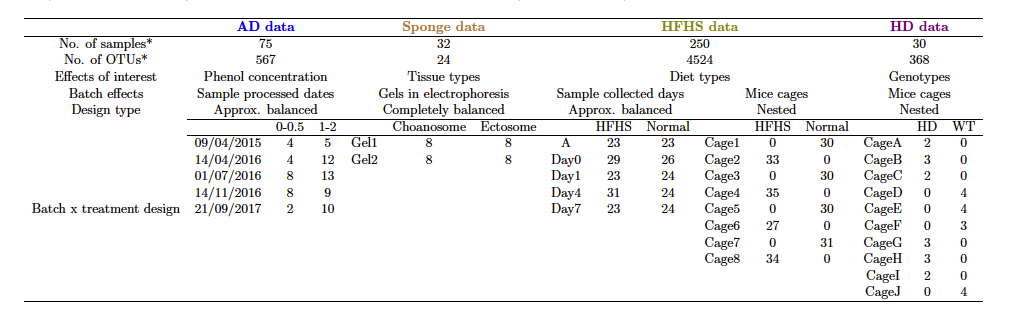
\includegraphics{./figures/data_description.png}
\textbf{Table 1: Overview of case studies with batch effects and their experimental designs.} We considered microbial studies for Anaerobic Digestion (\textcolor{blue}{AD data}), sponge \textit{A. aerophoba} (\textcolor{brown}{sponge data}), mice models with High Fat High Sugar diets (\textcolor{olive}{HFHS data}) and Huntington's Disease (\textcolor{violet}{HD data}).

\hypertarget{packages-installation-and-loading}{%
\section{Packages installation and loading}\label{packages-installation-and-loading}}

First, we load the packages necessary for analysis, and check the version of each package.

\begin{Shaded}
\begin{Highlighting}[]
\CommentTok{\# CRAN}
\NormalTok{cran.pkgs }\OtherTok{\textless{}{-}} \FunctionTok{c}\NormalTok{(}\StringTok{\textquotesingle{}pheatmap\textquotesingle{}}\NormalTok{, }\StringTok{\textquotesingle{}vegan\textquotesingle{}}\NormalTok{, }\StringTok{\textquotesingle{}ruv\textquotesingle{}}\NormalTok{, }\StringTok{\textquotesingle{}UpSetR\textquotesingle{}}\NormalTok{, }\StringTok{\textquotesingle{}gplots\textquotesingle{}}\NormalTok{, }
               \StringTok{\textquotesingle{}ggplot2\textquotesingle{}}\NormalTok{, }\StringTok{\textquotesingle{}gridExtra\textquotesingle{}}\NormalTok{, }\StringTok{\textquotesingle{}performance\textquotesingle{}}\NormalTok{, }\StringTok{\textquotesingle{}Rdpack\textquotesingle{}}\NormalTok{, }\StringTok{\textquotesingle{}pROC\textquotesingle{}}\NormalTok{)}
\CommentTok{\# Bioconductor}
\NormalTok{bioc.pkgs }\OtherTok{\textless{}{-}} \FunctionTok{c}\NormalTok{(}\StringTok{\textquotesingle{}mixOmics\textquotesingle{}}\NormalTok{, }\StringTok{\textquotesingle{}sva\textquotesingle{}}\NormalTok{, }\StringTok{\textquotesingle{}limma\textquotesingle{}}\NormalTok{, }\StringTok{\textquotesingle{}Biobase\textquotesingle{}}\NormalTok{, }\StringTok{\textquotesingle{}metagenomeSeq\textquotesingle{}}\NormalTok{)}
\CommentTok{\# GitHub}
\NormalTok{github.pkg }\OtherTok{\textless{}{-}} \StringTok{\textquotesingle{}PLSDAbatch\textquotesingle{}} 
\CommentTok{\# devtools::install\_github("https://github.com/EvaYiwenWang/PLSDAbatch")}

\CommentTok{\# built{-}in functions}
\FunctionTok{source}\NormalTok{(}\AttributeTok{file =} \StringTok{\textquotesingle{}./built\_in\_functions/data\_simulation.R\textquotesingle{}}\NormalTok{)}

\CommentTok{\# load packages }
\FunctionTok{sapply}\NormalTok{(}\FunctionTok{c}\NormalTok{(cran.pkgs, bioc.pkgs, github.pkg), require, }\AttributeTok{character.only =} \ConstantTok{TRUE}\NormalTok{)}
\end{Highlighting}
\end{Shaded}

\begin{verbatim}
##      pheatmap         vegan           ruv        UpSetR        gplots 
##          TRUE          TRUE          TRUE          TRUE          TRUE 
##       ggplot2     gridExtra   performance        Rdpack          pROC 
##          TRUE          TRUE          TRUE          TRUE          TRUE 
##      mixOmics           sva         limma       Biobase metagenomeSeq 
##          TRUE          TRUE          TRUE          TRUE          TRUE 
##    PLSDAbatch 
##          TRUE
\end{verbatim}

\begin{Shaded}
\begin{Highlighting}[]
\CommentTok{\# print package versions}
\FunctionTok{sapply}\NormalTok{(}\FunctionTok{c}\NormalTok{(cran.pkgs, bioc.pkgs, github.pkg), package.version)}
\end{Highlighting}
\end{Shaded}

\begin{verbatim}
##      pheatmap         vegan           ruv        UpSetR        gplots 
##      "1.0.12"       "2.6-4"     "0.9.7.1"       "1.4.0"       "3.1.3" 
##       ggplot2     gridExtra   performance        Rdpack          pROC 
##       "3.3.6"         "2.3"       "0.9.2"         "2.4"      "1.18.0" 
##      mixOmics           sva         limma       Biobase metagenomeSeq 
##      "6.20.0"      "3.44.0"      "3.52.2"      "2.56.0"      "1.38.0" 
##    PLSDAbatch 
##       "0.2.3"
\end{verbatim}

\hypertarget{data-pre-processing}{%
\section{Data pre-processing}\label{data-pre-processing}}

\hypertarget{pre-filtering}{%
\subsection{Pre-filtering}\label{pre-filtering}}

We load the \textcolor{blue}{AD data} stored internally with function \texttt{data()}.

\begin{Shaded}
\begin{Highlighting}[]
\CommentTok{\# AD data}
\FunctionTok{data}\NormalTok{(}\StringTok{\textquotesingle{}AD\_data\textquotesingle{}}\NormalTok{) }
\NormalTok{ad.count }\OtherTok{\textless{}{-}}\NormalTok{ AD\_data}\SpecialCharTok{$}\NormalTok{FullData}\SpecialCharTok{$}\NormalTok{X.count}
\FunctionTok{dim}\NormalTok{(ad.count)}
\end{Highlighting}
\end{Shaded}

\begin{verbatim}
## [1]  75 567
\end{verbatim}

The raw \textcolor{blue}{AD data} include 567 OTUs and 75 samples. We then use the function \texttt{PreFL()} from our \textcolor{orange}{PLSDAbatch} R package to filter the data.

\begin{Shaded}
\begin{Highlighting}[]
\NormalTok{ad.filter.res }\OtherTok{\textless{}{-}} \FunctionTok{PreFL}\NormalTok{(}\AttributeTok{data =}\NormalTok{ ad.count)}
\NormalTok{ad.filter }\OtherTok{\textless{}{-}}\NormalTok{ ad.filter.res}\SpecialCharTok{$}\NormalTok{data.filter}
\FunctionTok{dim}\NormalTok{(ad.filter)}
\end{Highlighting}
\end{Shaded}

\begin{verbatim}
## [1]  75 231
\end{verbatim}

\begin{Shaded}
\begin{Highlighting}[]
\CommentTok{\# zero proportion before filtering}
\NormalTok{ad.filter.res}\SpecialCharTok{$}\NormalTok{zero.prob}
\end{Highlighting}
\end{Shaded}

\begin{verbatim}
## [1] 0.6328042
\end{verbatim}

\begin{Shaded}
\begin{Highlighting}[]
\CommentTok{\# zero proportion after filtering}
\FunctionTok{sum}\NormalTok{(ad.filter }\SpecialCharTok{==} \DecValTok{0}\NormalTok{)}\SpecialCharTok{/}\NormalTok{(}\FunctionTok{nrow}\NormalTok{(ad.filter) }\SpecialCharTok{*} \FunctionTok{ncol}\NormalTok{(ad.filter))}
\end{Highlighting}
\end{Shaded}

\begin{verbatim}
## [1] 0.3806638
\end{verbatim}

After filtering, 231 OTUs remained, and the proportion of zeroes decreased from 63\% to 38\%.

We can also load the other data, such as the \textcolor{brown}{sponge data}.

\begin{Shaded}
\begin{Highlighting}[]
\CommentTok{\# Sponge data}
\FunctionTok{data}\NormalTok{(}\StringTok{\textquotesingle{}sponge\_data\textquotesingle{}}\NormalTok{) }
\NormalTok{sponge.tss }\OtherTok{\textless{}{-}}\NormalTok{ sponge\_data}\SpecialCharTok{$}\NormalTok{X.tss}
\FunctionTok{dim}\NormalTok{(sponge.tss)}
\end{Highlighting}
\end{Shaded}

\begin{verbatim}
## [1] 32 24
\end{verbatim}

\begin{Shaded}
\begin{Highlighting}[]
\CommentTok{\# zero proportion}
\FunctionTok{sum}\NormalTok{(sponge.tss }\SpecialCharTok{==} \DecValTok{0}\NormalTok{)}\SpecialCharTok{/}\NormalTok{(}\FunctionTok{nrow}\NormalTok{(sponge.tss) }\SpecialCharTok{*} \FunctionTok{ncol}\NormalTok{(sponge.tss))}
\end{Highlighting}
\end{Shaded}

\begin{verbatim}
## [1] 0.5455729
\end{verbatim}

The \textcolor{brown}{sponge data} include the relative abundance of 24 OTUs and 32 samples. Given the small number of OTUs, we advise not to pre-filter the data.

Note: The \texttt{PreFL()} function is only dedicated to raw counts, rather than relative abundance data. We also recommend to start the pre-filtering on raw counts, rather than relative abundance data to mitigate the compositionality issue.

\hypertarget{transformation}{%
\subsection{Transformation}\label{transformation}}

Prior to CLR transformation, we recommend adding 1 as the offset for the \textcolor{blue}{AD data} - that are raw count data, and 0.01 as the offset for the \textcolor{brown}{sponge data} - that are relative abundance data. We use \texttt{logratio.transfo()} function in \textcolor{orange}{mixOmics} package to CLR transform the data.

\begin{Shaded}
\begin{Highlighting}[]
\NormalTok{ad.clr }\OtherTok{\textless{}{-}} \FunctionTok{logratio.transfo}\NormalTok{(}\AttributeTok{X =}\NormalTok{ ad.filter, }\AttributeTok{logratio =} \StringTok{\textquotesingle{}CLR\textquotesingle{}}\NormalTok{, }\AttributeTok{offset =} \DecValTok{1}\NormalTok{) }
\FunctionTok{class}\NormalTok{(ad.clr) }\OtherTok{=} \StringTok{\textquotesingle{}matrix\textquotesingle{}}

\NormalTok{sponge.clr }\OtherTok{\textless{}{-}} \FunctionTok{logratio.transfo}\NormalTok{(}\AttributeTok{X =}\NormalTok{ sponge.tss, }\AttributeTok{logratio =} \StringTok{\textquotesingle{}CLR\textquotesingle{}}\NormalTok{, }\AttributeTok{offset =} \FloatTok{0.01}\NormalTok{)}
\FunctionTok{class}\NormalTok{(sponge.clr) }\OtherTok{=} \StringTok{\textquotesingle{}matrix\textquotesingle{}}
\end{Highlighting}
\end{Shaded}

\hypertarget{batch-effect-detection}{%
\section{Batch effect detection}\label{batch-effect-detection}}

\hypertarget{pca}{%
\subsection{PCA}\label{pca}}

We apply \texttt{pca()} function from \textcolor{orange}{mixOmics} package to the \textcolor{blue}{AD data} and \texttt{Scatter\_Density()} function from \textcolor{orange}{PLSDAbatch} to represent the PCA sample plot with densities.

\begin{Shaded}
\begin{Highlighting}[]
\CommentTok{\# AD data}
\NormalTok{ad.pca.before }\OtherTok{\textless{}{-}} \FunctionTok{pca}\NormalTok{(ad.clr, }\AttributeTok{ncomp =} \DecValTok{3}\NormalTok{, }\AttributeTok{scale =} \ConstantTok{TRUE}\NormalTok{)}

\NormalTok{ad.metadata }\OtherTok{\textless{}{-}}\NormalTok{ AD\_data}\SpecialCharTok{$}\NormalTok{FullData}\SpecialCharTok{$}\NormalTok{metadata}
\NormalTok{ad.batch }\OtherTok{=} \FunctionTok{factor}\NormalTok{(ad.metadata}\SpecialCharTok{$}\NormalTok{sequencing\_run\_date, }
                  \AttributeTok{levels =} \FunctionTok{unique}\NormalTok{(ad.metadata}\SpecialCharTok{$}\NormalTok{sequencing\_run\_date))}
\NormalTok{ad.trt }\OtherTok{=} \FunctionTok{as.factor}\NormalTok{(ad.metadata}\SpecialCharTok{$}\NormalTok{initial\_phenol\_concentration.regroup)}
\FunctionTok{names}\NormalTok{(ad.batch) }\OtherTok{\textless{}{-}} \FunctionTok{names}\NormalTok{(ad.trt) }\OtherTok{\textless{}{-}} \FunctionTok{rownames}\NormalTok{(ad.metadata)}

\FunctionTok{Scatter\_Density}\NormalTok{(}\AttributeTok{object =}\NormalTok{ ad.pca.before, }\AttributeTok{batch =}\NormalTok{ ad.batch, }\AttributeTok{trt =}\NormalTok{ ad.trt, }
                \AttributeTok{title =} \StringTok{\textquotesingle{}AD data\textquotesingle{}}\NormalTok{, }\AttributeTok{trt.legend.title =} \StringTok{\textquotesingle{}Phenol conc.\textquotesingle{}}\NormalTok{)}
\end{Highlighting}
\end{Shaded}

\begin{figure}

{\centering 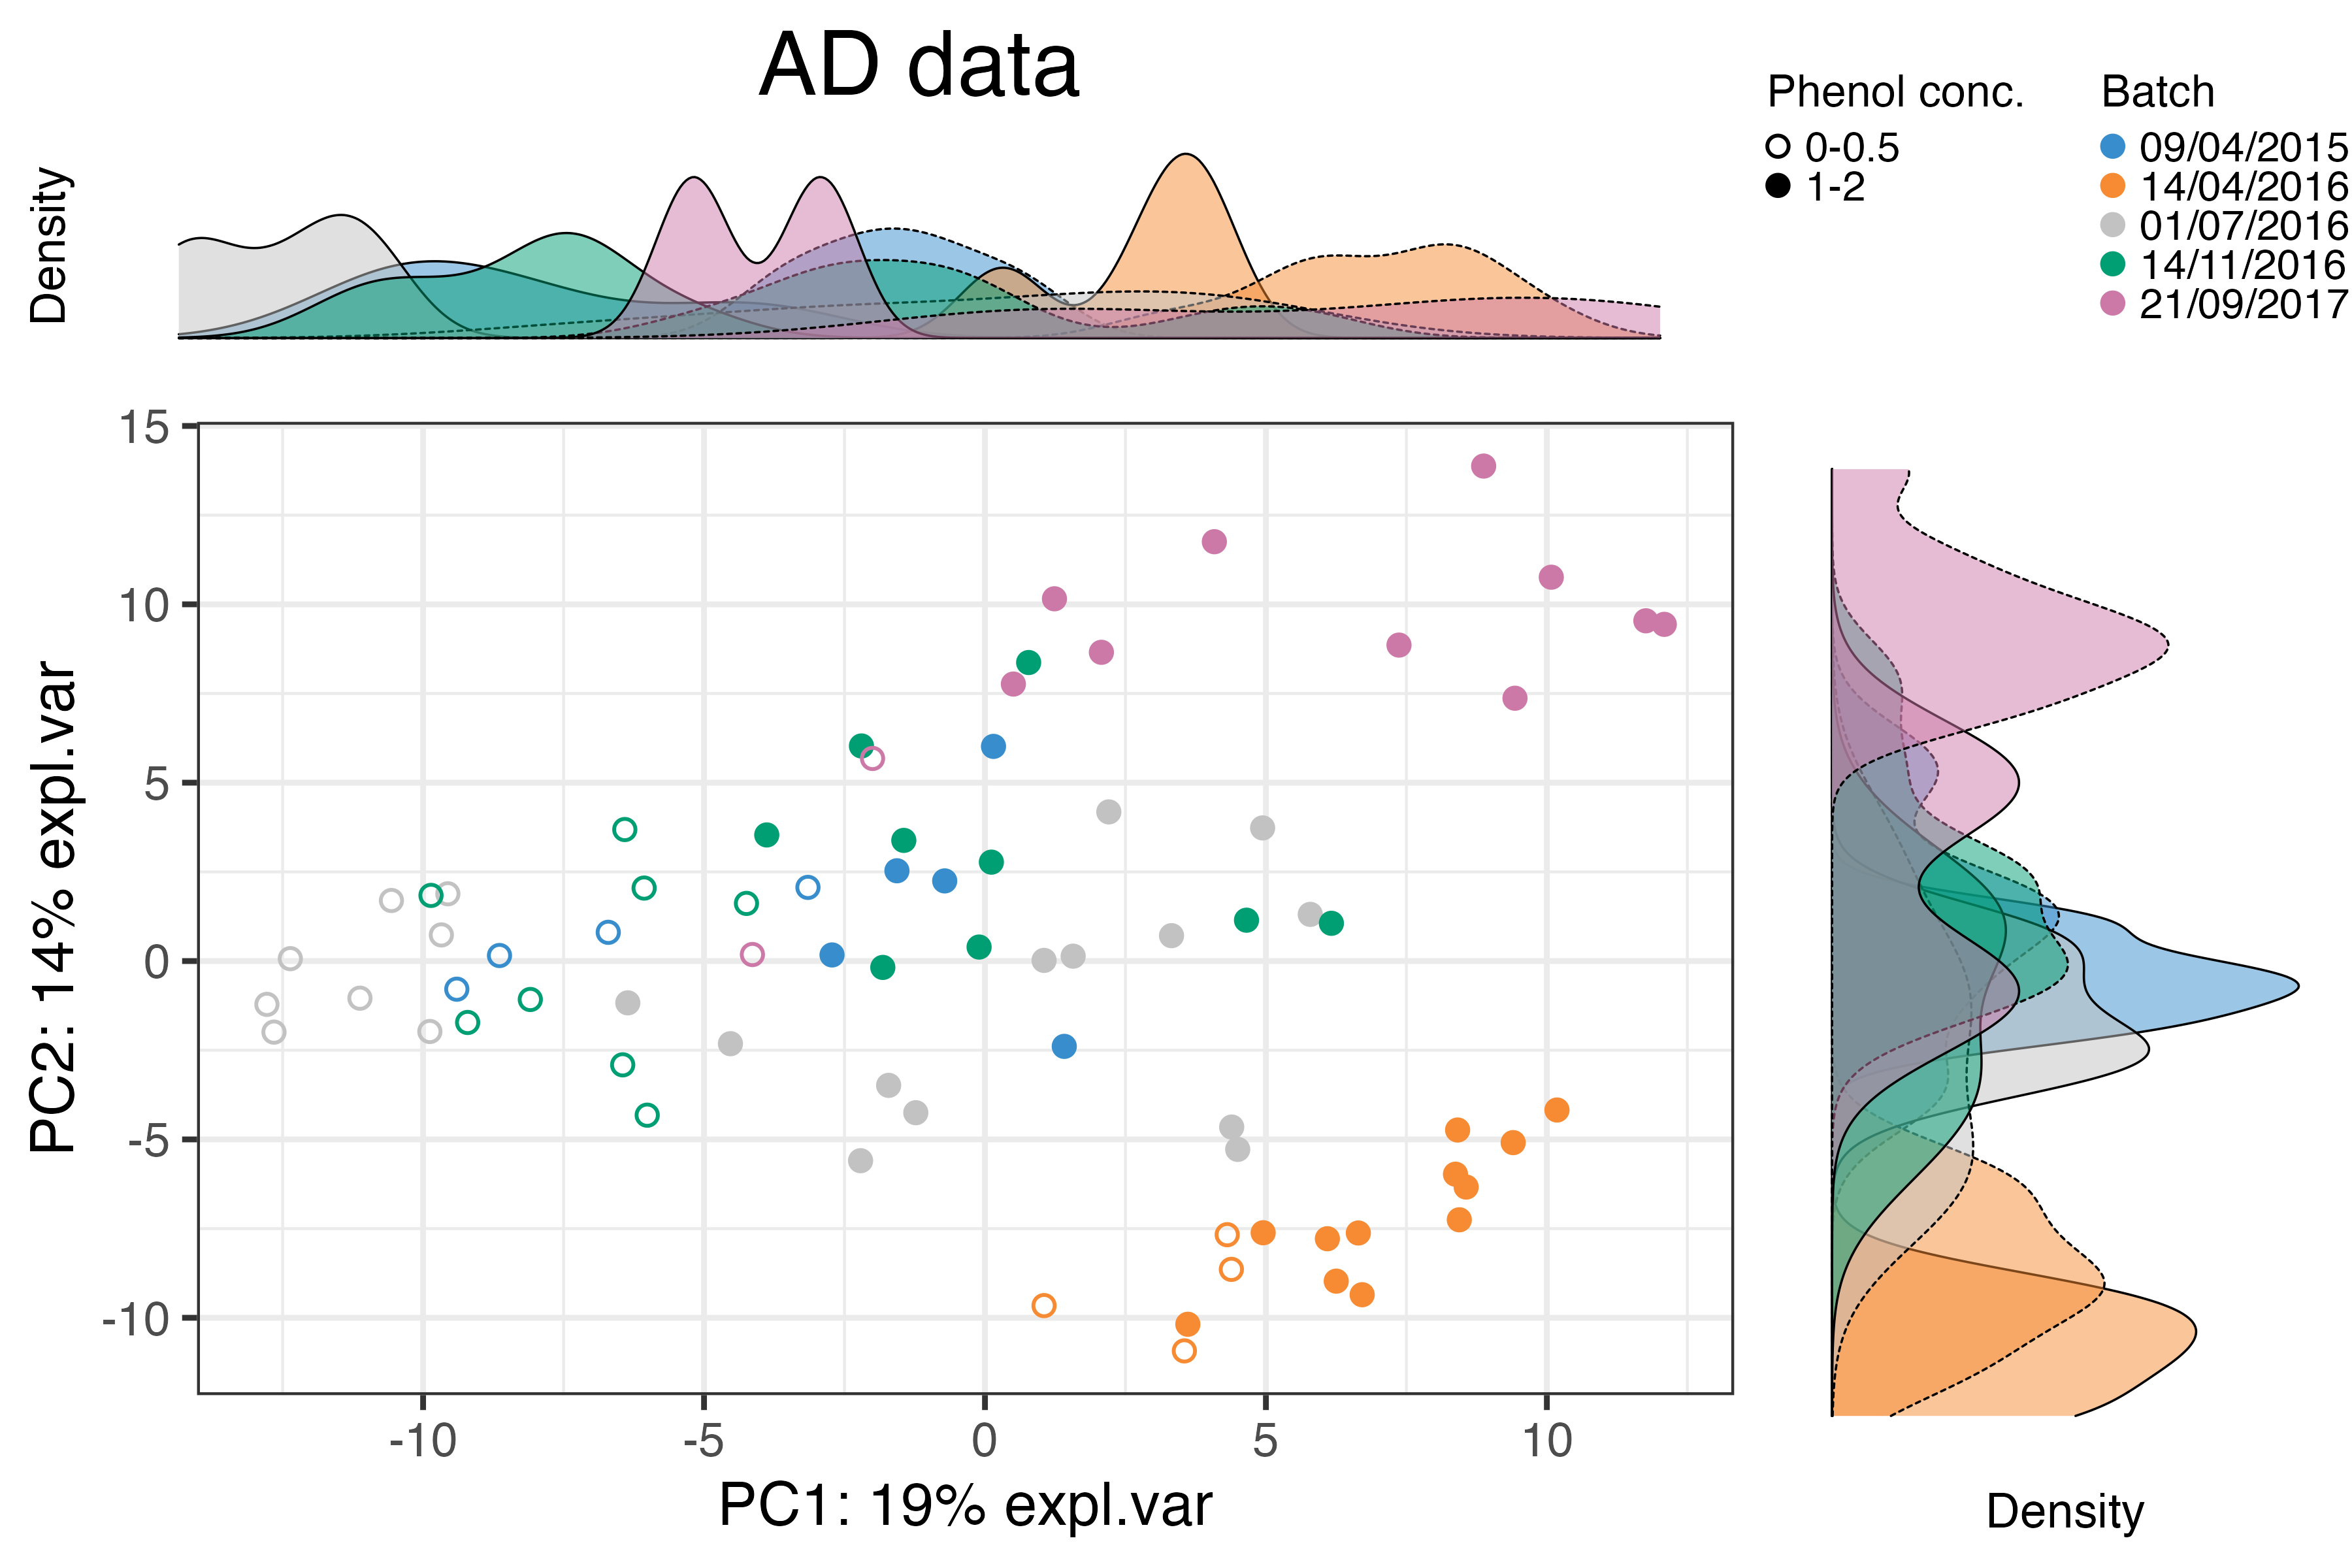
\includegraphics[width=0.6\linewidth]{PLSDAbatch_workflow_files/figure-latex/ADpcaBefore-1} 

}

\caption{The PCA sample plot with densities in the AD data.}\label{fig:ADpcaBefore}
\end{figure}

In the above figure, we observed 1) the distinction between samples treated with different phenol concentrations and 2) the differences between samples sequenced at ``14/04/2016'', ``21/09/2017'' and the other dates. Therefore, the batch effect related to dates needs to be removed.

\hypertarget{boxplots-and-density-plots}{%
\subsection{Boxplots and density plots}\label{boxplots-and-density-plots}}

We first identify the top OTU driving the major variance in PCA using \texttt{selectVar()} in \textcolor{orange}{mixOmics} package. Each identified OTU can then be plotted as boxplots and density plots using \texttt{box\_plot()} and \texttt{density\_plot()} in \textcolor{orange}{PLSDAbatch}.

\begin{Shaded}
\begin{Highlighting}[]
\NormalTok{ad.OTU.name }\OtherTok{\textless{}{-}} \FunctionTok{selectVar}\NormalTok{(ad.pca.before, }\AttributeTok{comp =} \DecValTok{1}\NormalTok{)}\SpecialCharTok{$}\NormalTok{name[}\DecValTok{1}\NormalTok{]}
\NormalTok{ad.OTU\_batch }\OtherTok{\textless{}{-}} \FunctionTok{data.frame}\NormalTok{(}\AttributeTok{value =}\NormalTok{ ad.clr[,ad.OTU.name], }\AttributeTok{batch =}\NormalTok{ ad.batch)}
\FunctionTok{box\_plot}\NormalTok{(}\AttributeTok{df =}\NormalTok{ ad.OTU\_batch, }\AttributeTok{title =} \FunctionTok{paste}\NormalTok{(ad.OTU.name, }\StringTok{\textquotesingle{}(AD data)\textquotesingle{}}\NormalTok{), }
         \AttributeTok{x.angle =} \DecValTok{30}\NormalTok{)}
\end{Highlighting}
\end{Shaded}

\begin{figure}

{\centering 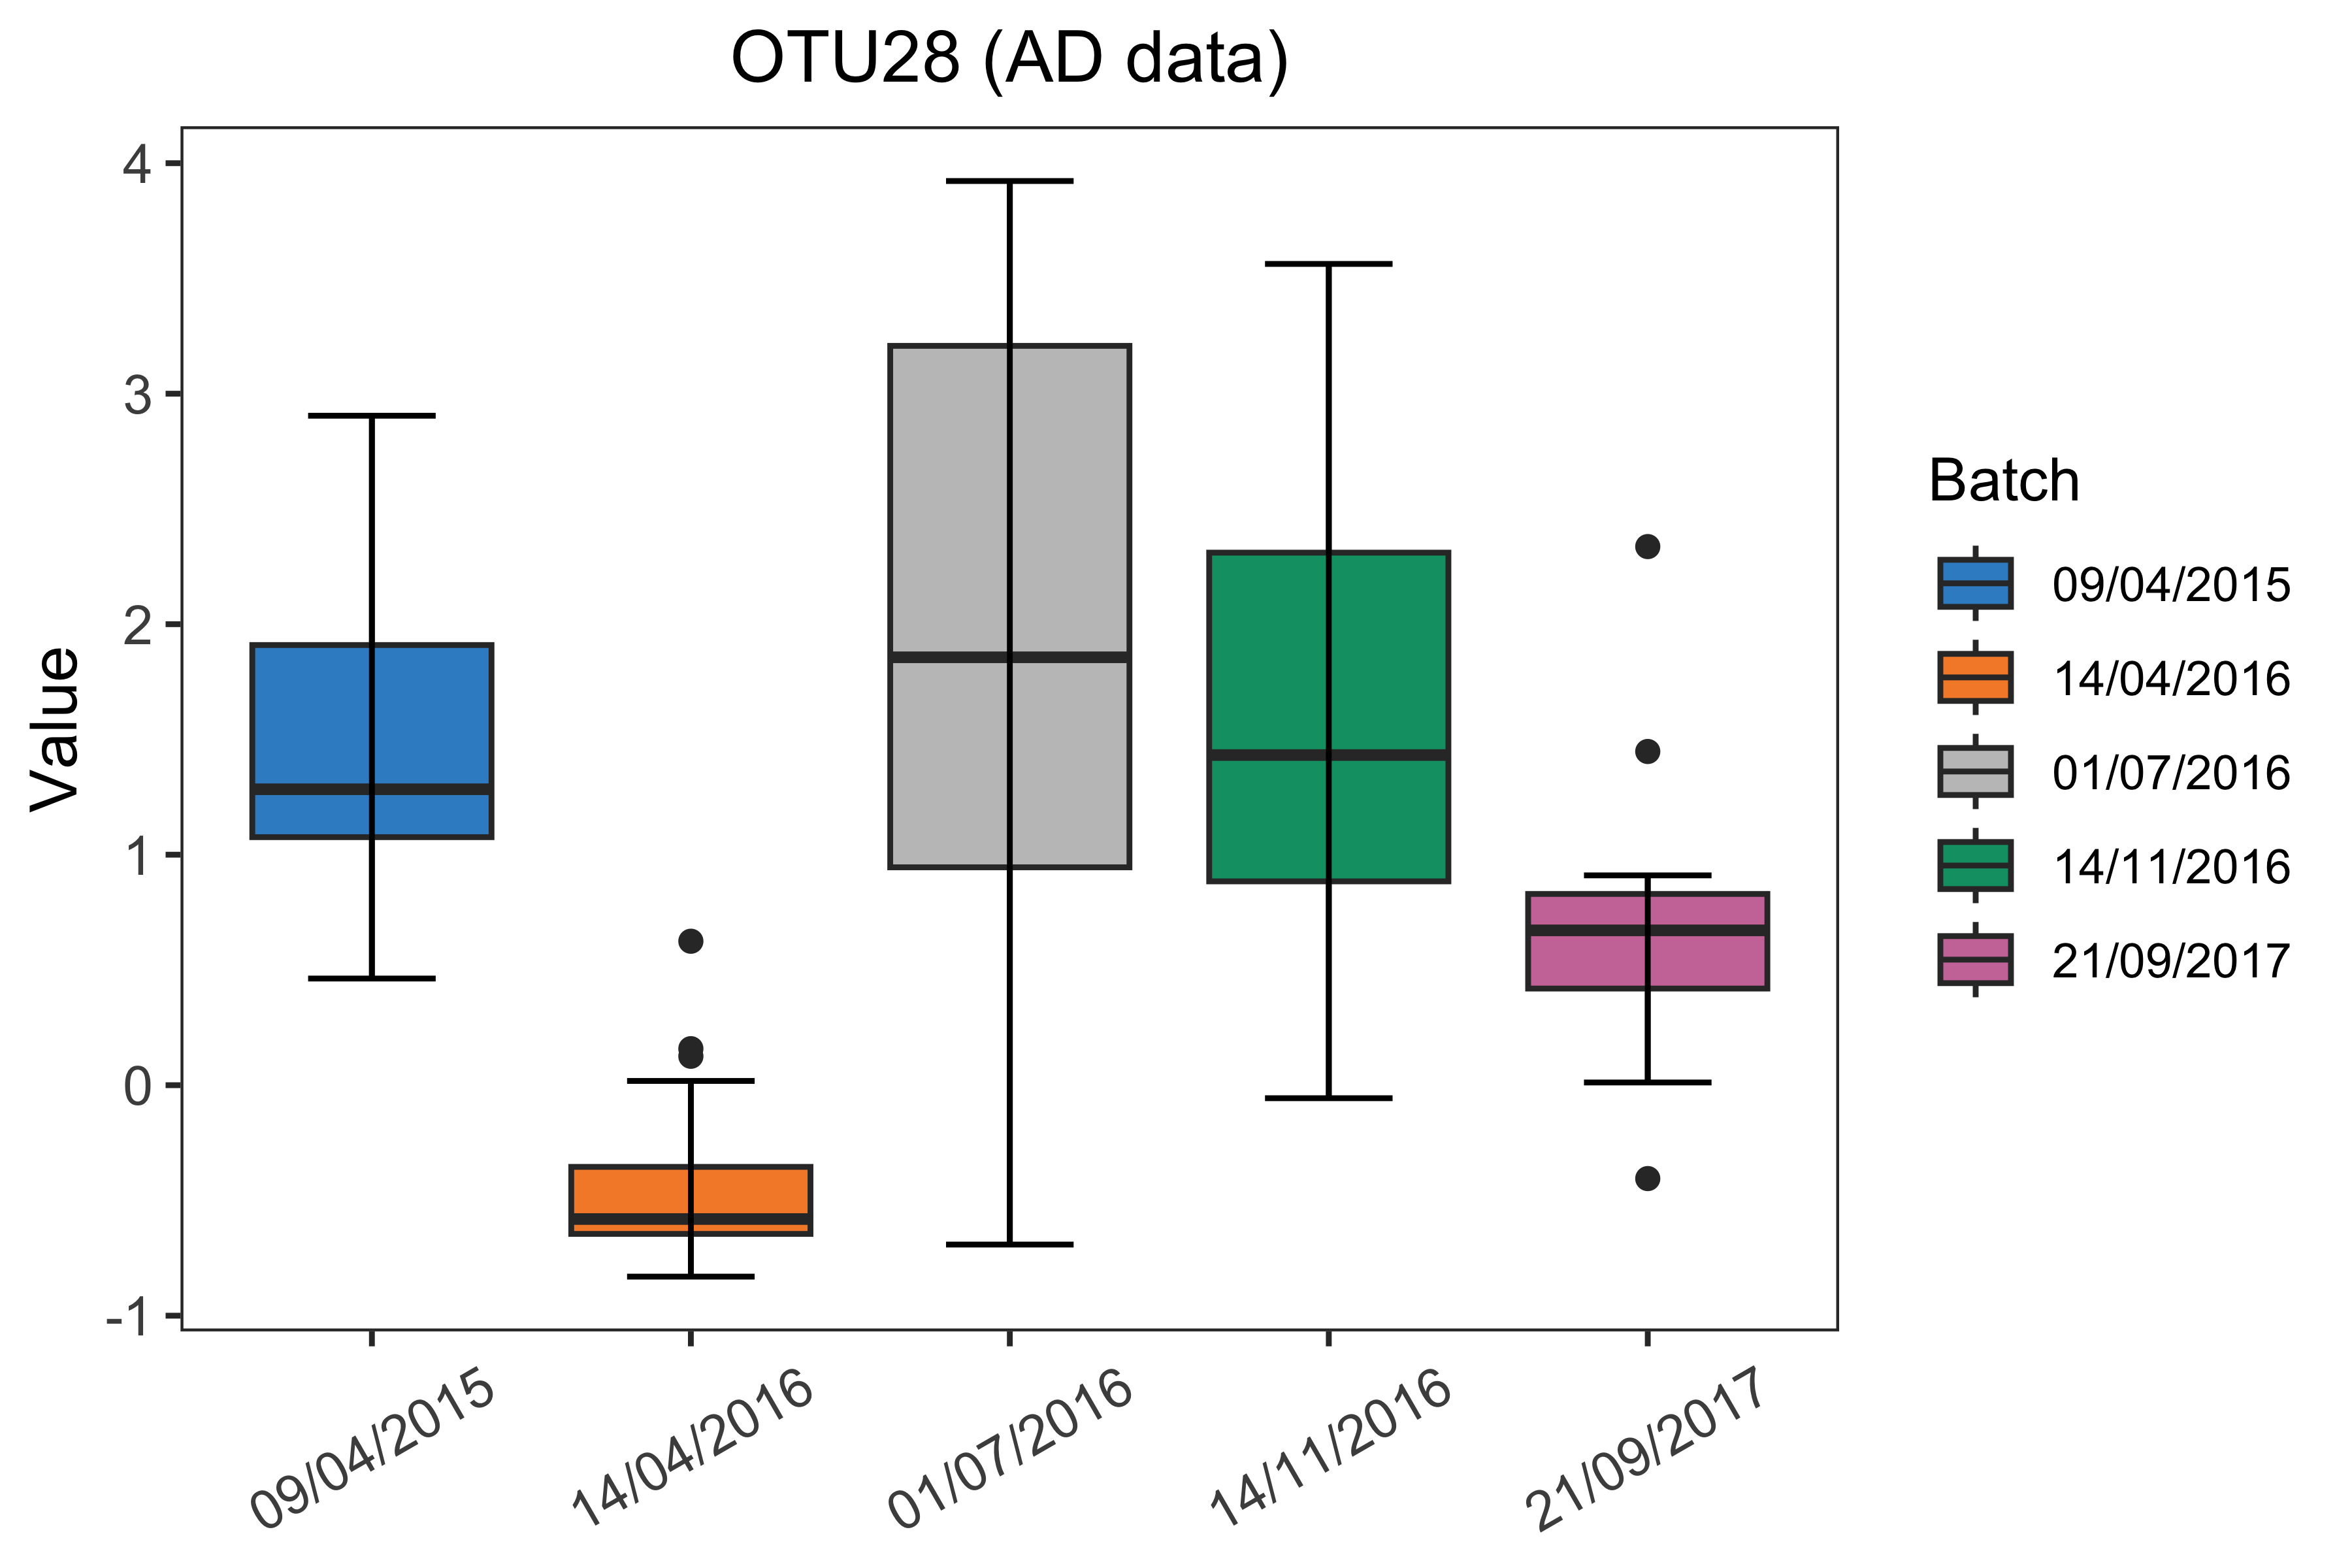
\includegraphics[width=0.6\linewidth]{PLSDAbatch_workflow_files/figure-latex/ADboxBefore-1} 

}

\caption{Boxplots of sample values in "OTU28" before batch effect correction in the AD data.}\label{fig:ADboxBefore}
\end{figure}

\begin{Shaded}
\begin{Highlighting}[]
\FunctionTok{density\_plot}\NormalTok{(}\AttributeTok{df =}\NormalTok{ ad.OTU\_batch, }\AttributeTok{title =} \FunctionTok{paste}\NormalTok{(ad.OTU.name, }\StringTok{\textquotesingle{}(AD data)\textquotesingle{}}\NormalTok{))}
\end{Highlighting}
\end{Shaded}

\begin{figure}

{\centering 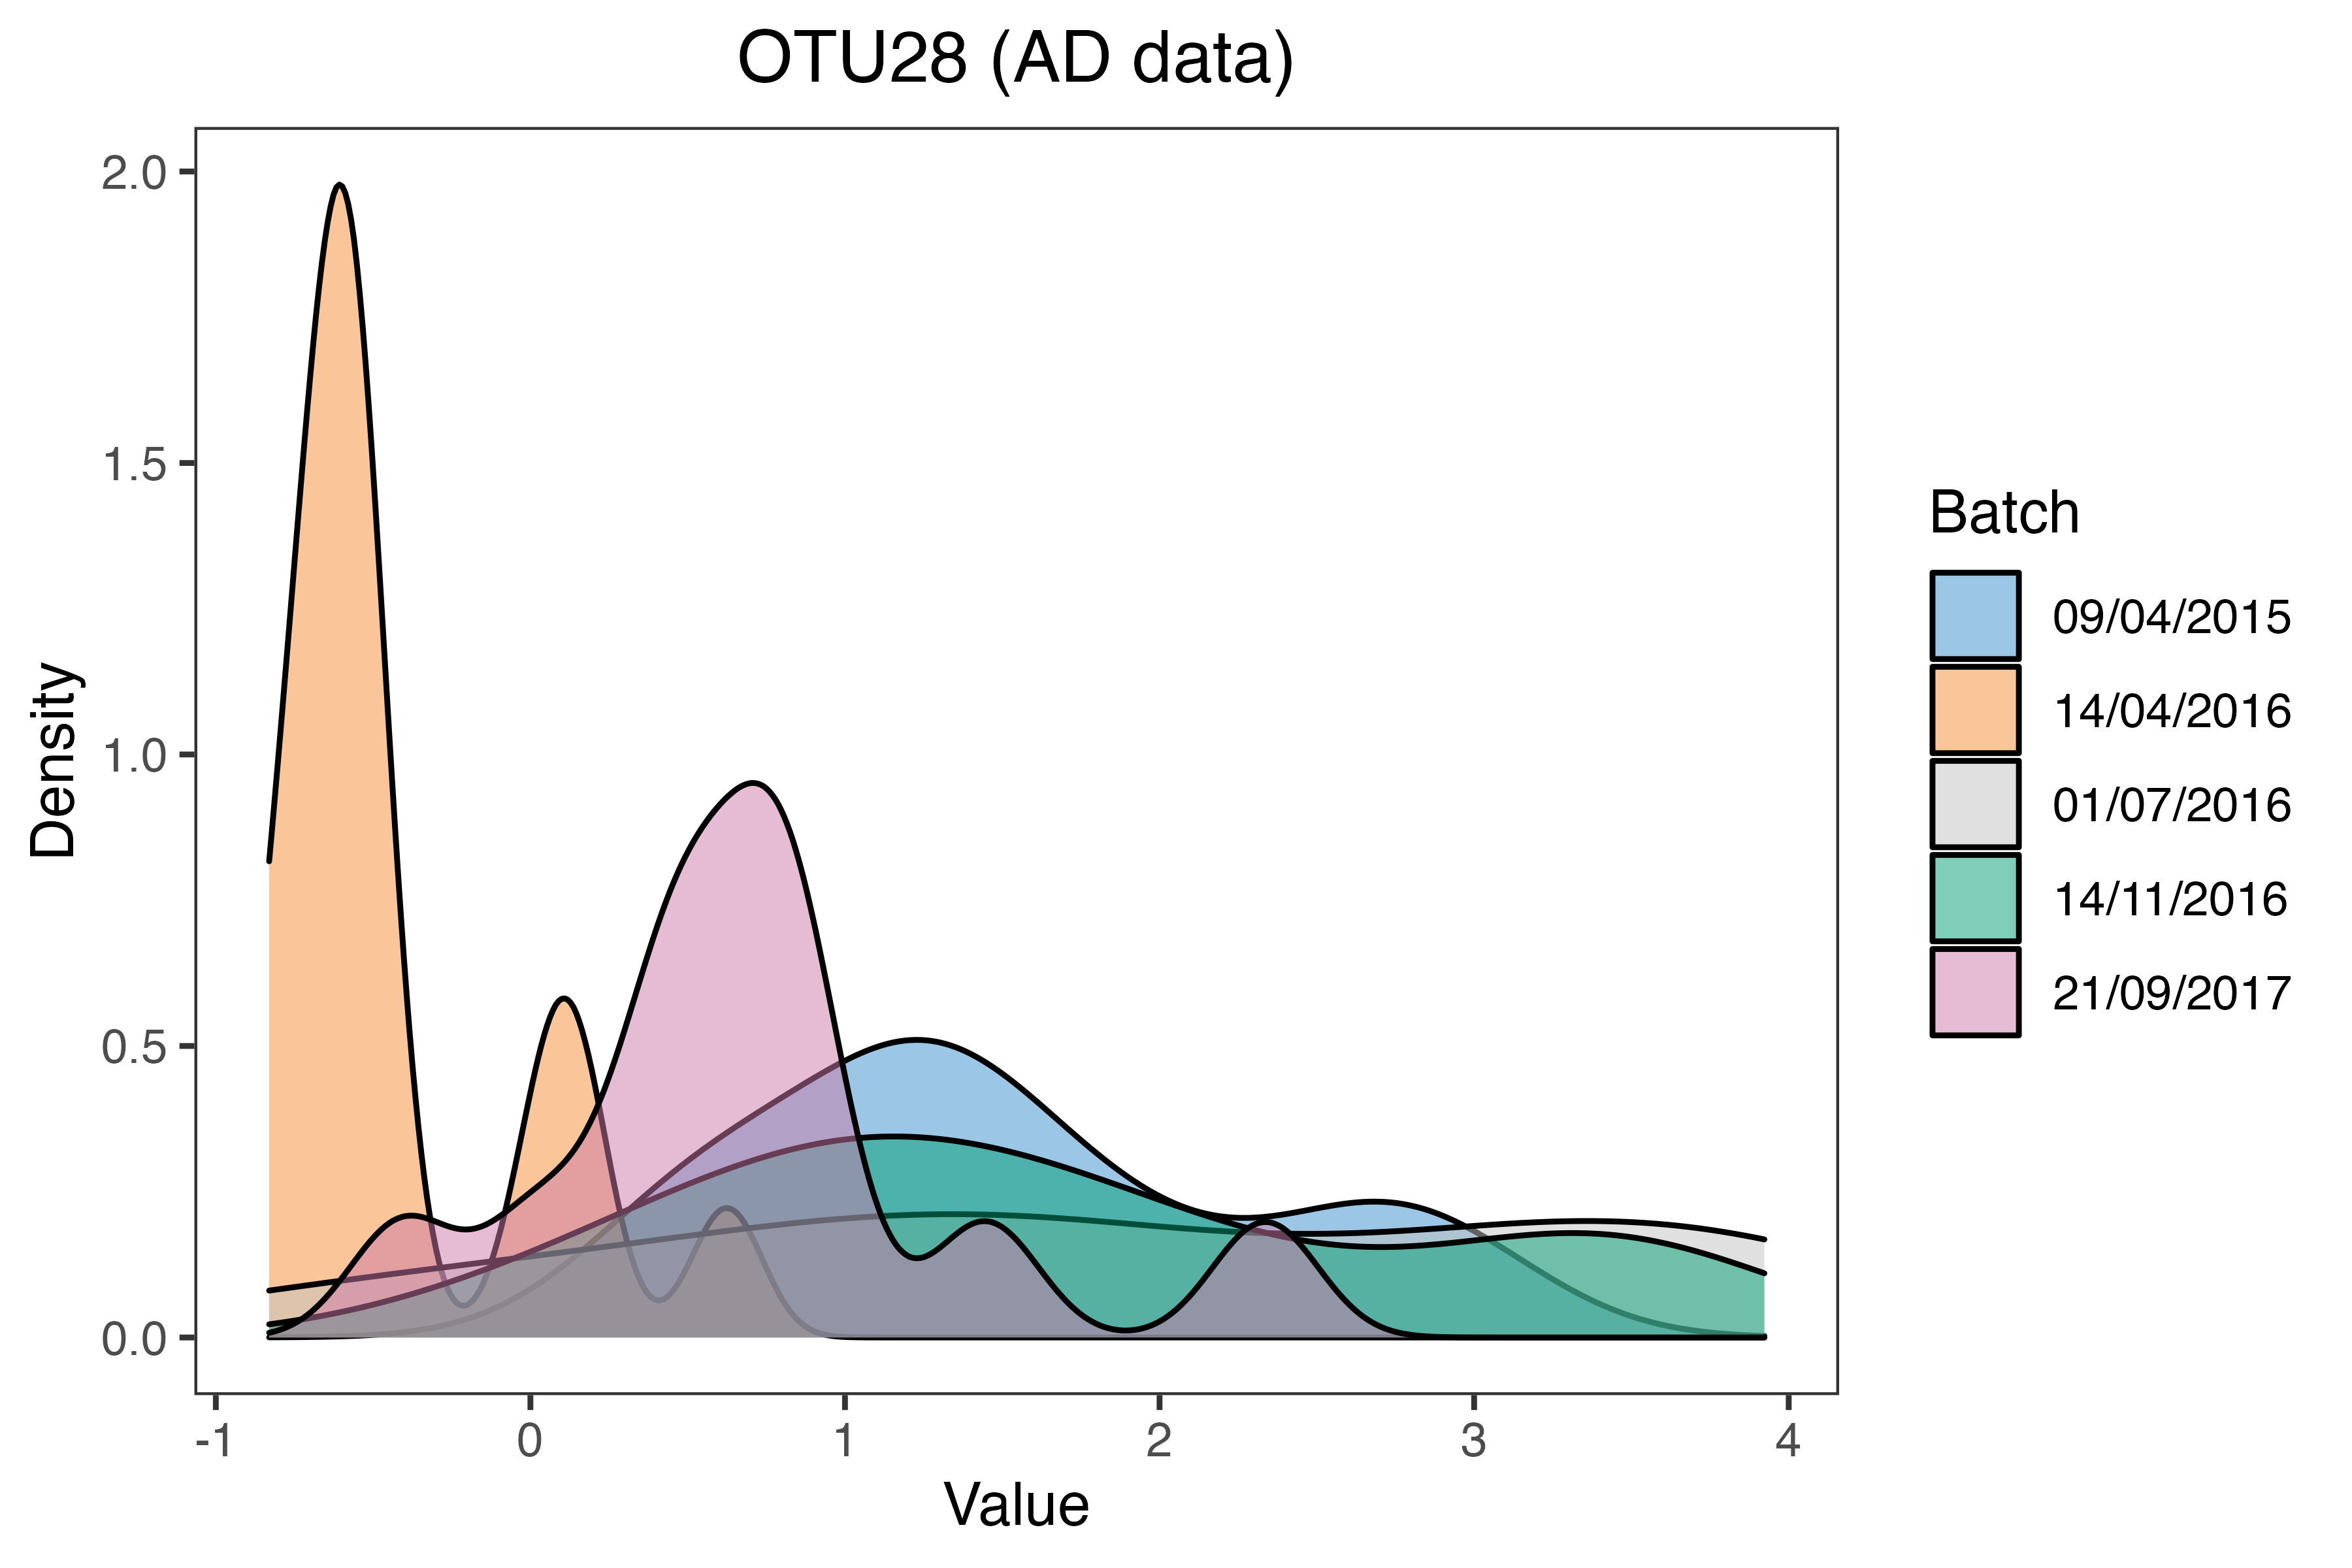
\includegraphics[width=0.6\linewidth]{PLSDAbatch_workflow_files/figure-latex/ADdensityBefore-1} 

}

\caption{Density plots of sample values in "OTU28" before batch effect correction in the AD data.}\label{fig:ADdensityBefore}
\end{figure}

The boxplot and density plot indicated a strong date batch effect because of the differences between ``14/04/2016'', ``21/09/2017'' and the other dates in the ``OTU28''.

We also apply a linear regression model to the ``OTU28'' using \texttt{linear\_regres()} from \textcolor{orange}{PLSDAbatch} with batch and treatment effects as covariates. We set ``14/04/2016'' and ``21/09/2017'' as the reference batch respectively with \texttt{relevel()} from \textcolor{orange}{stats}.

\begin{Shaded}
\begin{Highlighting}[]
\CommentTok{\# reference batch: 14/04/2016}
\NormalTok{ad.batch }\OtherTok{\textless{}{-}} \FunctionTok{relevel}\NormalTok{(}\AttributeTok{x =}\NormalTok{ ad.batch, }\AttributeTok{ref =} \StringTok{\textquotesingle{}14/04/2016\textquotesingle{}}\NormalTok{)}

\NormalTok{ad.OTU.lm }\OtherTok{\textless{}{-}} \FunctionTok{linear\_regres}\NormalTok{(}\AttributeTok{data =}\NormalTok{ ad.clr[,ad.OTU.name], }
                           \AttributeTok{trt =}\NormalTok{ ad.trt, }\AttributeTok{batch.fix =}\NormalTok{ ad.batch, }
                           \AttributeTok{type =} \StringTok{\textquotesingle{}linear model\textquotesingle{}}\NormalTok{)}
\FunctionTok{summary}\NormalTok{(ad.OTU.lm}\SpecialCharTok{$}\NormalTok{model}\SpecialCharTok{$}\NormalTok{data)}
\end{Highlighting}
\end{Shaded}

\begin{verbatim}
## 
## Call:
## lm(formula = data[, i] ~ trt + batch.fix)
## 
## Residuals:
##     Min      1Q  Median      3Q     Max 
## -1.9384 -0.3279  0.1635  0.3849  0.9887 
## 
## Coefficients:
##                     Estimate Std. Error t value Pr(>|t|)    
## (Intercept)           0.8501     0.2196   3.871 0.000243 ***
## trt1-2               -1.6871     0.1754  -9.617 2.27e-14 ***
## batch.fix09/04/2015   1.5963     0.2950   5.410 8.55e-07 ***
## batch.fix01/07/2016   2.0839     0.2345   8.886 4.82e-13 ***
## batch.fix14/11/2016   1.7405     0.2480   7.018 1.24e-09 ***
## batch.fix21/09/2017   1.2646     0.2690   4.701 1.28e-05 ***
## ---
## Signif. codes:  0 '***' 0.001 '**' 0.01 '*' 0.05 '.' 0.1 ' ' 1
## 
## Residual standard error: 0.7033 on 69 degrees of freedom
## Multiple R-squared:  0.7546, Adjusted R-squared:  0.7368 
## F-statistic: 42.44 on 5 and 69 DF,  p-value: < 2.2e-16
\end{verbatim}

\begin{Shaded}
\begin{Highlighting}[]
\CommentTok{\# reference batch: 21/09/2017}
\NormalTok{ad.batch }\OtherTok{\textless{}{-}} \FunctionTok{relevel}\NormalTok{(}\AttributeTok{x =}\NormalTok{ ad.batch, }\AttributeTok{ref =} \StringTok{\textquotesingle{}21/09/2017\textquotesingle{}}\NormalTok{)}

\NormalTok{ad.OTU.lm }\OtherTok{\textless{}{-}} \FunctionTok{linear\_regres}\NormalTok{(}\AttributeTok{data =}\NormalTok{ ad.clr[,ad.OTU.name], }
                           \AttributeTok{trt =}\NormalTok{ ad.trt, }\AttributeTok{batch.fix =}\NormalTok{ ad.batch, }
                           \AttributeTok{type =} \StringTok{\textquotesingle{}linear model\textquotesingle{}}\NormalTok{)}
\FunctionTok{summary}\NormalTok{(ad.OTU.lm}\SpecialCharTok{$}\NormalTok{model}\SpecialCharTok{$}\NormalTok{data)}
\end{Highlighting}
\end{Shaded}

\begin{verbatim}
## 
## Call:
## lm(formula = data[, i] ~ trt + batch.fix)
## 
## Residuals:
##     Min      1Q  Median      3Q     Max 
## -1.9384 -0.3279  0.1635  0.3849  0.9887 
## 
## Coefficients:
##                     Estimate Std. Error t value Pr(>|t|)    
## (Intercept)           2.1147     0.2502   8.453 2.97e-12 ***
## trt1-2               -1.6871     0.1754  -9.617 2.27e-14 ***
## batch.fix14/04/2016  -1.2646     0.2690  -4.701 1.28e-05 ***
## batch.fix09/04/2015   0.3317     0.3139   1.056  0.29446    
## batch.fix01/07/2016   0.8193     0.2573   3.185  0.00218 ** 
## batch.fix14/11/2016   0.4759     0.2705   1.760  0.08292 .  
## ---
## Signif. codes:  0 '***' 0.001 '**' 0.01 '*' 0.05 '.' 0.1 ' ' 1
## 
## Residual standard error: 0.7033 on 69 degrees of freedom
## Multiple R-squared:  0.7546, Adjusted R-squared:  0.7368 
## F-statistic: 42.44 on 5 and 69 DF,  p-value: < 2.2e-16
\end{verbatim}

From the results of linear regression, we observed P \textless{} 0.001 for the regression coefficients associated with all the other batches when the reference batch was ``14/04/2016'', which confirmed the difference between the samples from batch ``14/04/2016'' and the other samples as observed from previous plots. When the reference batch was ``21/09/2017'', we also observed significant differences between batch ``21/09/2017'' and ``14/04/2016'', between ``21/09/2017'' and ``01/07/2016''. Therefore, the batch effect because of ``21/09/2017'' also exists.

\hypertarget{heatmap}{%
\subsection{Heatmap}\label{heatmap}}

We produce a heatmap using \textcolor{orange}{pheatmap} package. The data first need to be scaled on both OTUs and samples.

\begin{Shaded}
\begin{Highlighting}[]
\CommentTok{\# scale the clr data on both OTUs and samples}
\NormalTok{ad.clr.s }\OtherTok{\textless{}{-}} \FunctionTok{scale}\NormalTok{(ad.clr, }\AttributeTok{center =} \ConstantTok{TRUE}\NormalTok{, }\AttributeTok{scale =} \ConstantTok{TRUE}\NormalTok{)}
\NormalTok{ad.clr.ss }\OtherTok{\textless{}{-}} \FunctionTok{scale}\NormalTok{(}\FunctionTok{t}\NormalTok{(ad.clr.s), }\AttributeTok{center =} \ConstantTok{TRUE}\NormalTok{, }\AttributeTok{scale =} \ConstantTok{TRUE}\NormalTok{)}

\NormalTok{ad.anno\_col }\OtherTok{\textless{}{-}} \FunctionTok{data.frame}\NormalTok{(}\AttributeTok{Batch =}\NormalTok{ ad.batch, }\AttributeTok{Treatment =}\NormalTok{ ad.trt)}
\NormalTok{ad.anno\_colors }\OtherTok{\textless{}{-}} \FunctionTok{list}\NormalTok{(}\AttributeTok{Batch =} \FunctionTok{color.mixo}\NormalTok{(}\FunctionTok{seq\_len}\NormalTok{(}\DecValTok{5}\NormalTok{)), }
                       \AttributeTok{Treatment =} \FunctionTok{pb\_color}\NormalTok{(}\FunctionTok{seq\_len}\NormalTok{(}\DecValTok{2}\NormalTok{)))}
\FunctionTok{names}\NormalTok{(ad.anno\_colors}\SpecialCharTok{$}\NormalTok{Batch) }\OtherTok{=} \FunctionTok{levels}\NormalTok{(ad.batch)}
\FunctionTok{names}\NormalTok{(ad.anno\_colors}\SpecialCharTok{$}\NormalTok{Treatment) }\OtherTok{=} \FunctionTok{levels}\NormalTok{(ad.trt)}

\FunctionTok{pheatmap}\NormalTok{(ad.clr.ss, }
         \AttributeTok{cluster\_rows =} \ConstantTok{FALSE}\NormalTok{, }
         \AttributeTok{fontsize\_row =} \DecValTok{4}\NormalTok{, }
         \AttributeTok{fontsize\_col =} \DecValTok{6}\NormalTok{,}
         \AttributeTok{fontsize =} \DecValTok{8}\NormalTok{,}
         \AttributeTok{clustering\_distance\_rows =} \StringTok{\textquotesingle{}euclidean\textquotesingle{}}\NormalTok{,}
         \AttributeTok{clustering\_method =} \StringTok{\textquotesingle{}ward.D\textquotesingle{}}\NormalTok{,}
         \AttributeTok{treeheight\_row =} \DecValTok{30}\NormalTok{,}
         \AttributeTok{annotation\_col =}\NormalTok{ ad.anno\_col,}
         \AttributeTok{annotation\_colors =}\NormalTok{ ad.anno\_colors,}
         \AttributeTok{border\_color =} \StringTok{\textquotesingle{}NA\textquotesingle{}}\NormalTok{,}
         \AttributeTok{main =} \StringTok{\textquotesingle{}AD data {-} Scaled\textquotesingle{}}\NormalTok{)}
\end{Highlighting}
\end{Shaded}

\begin{figure}

{\centering 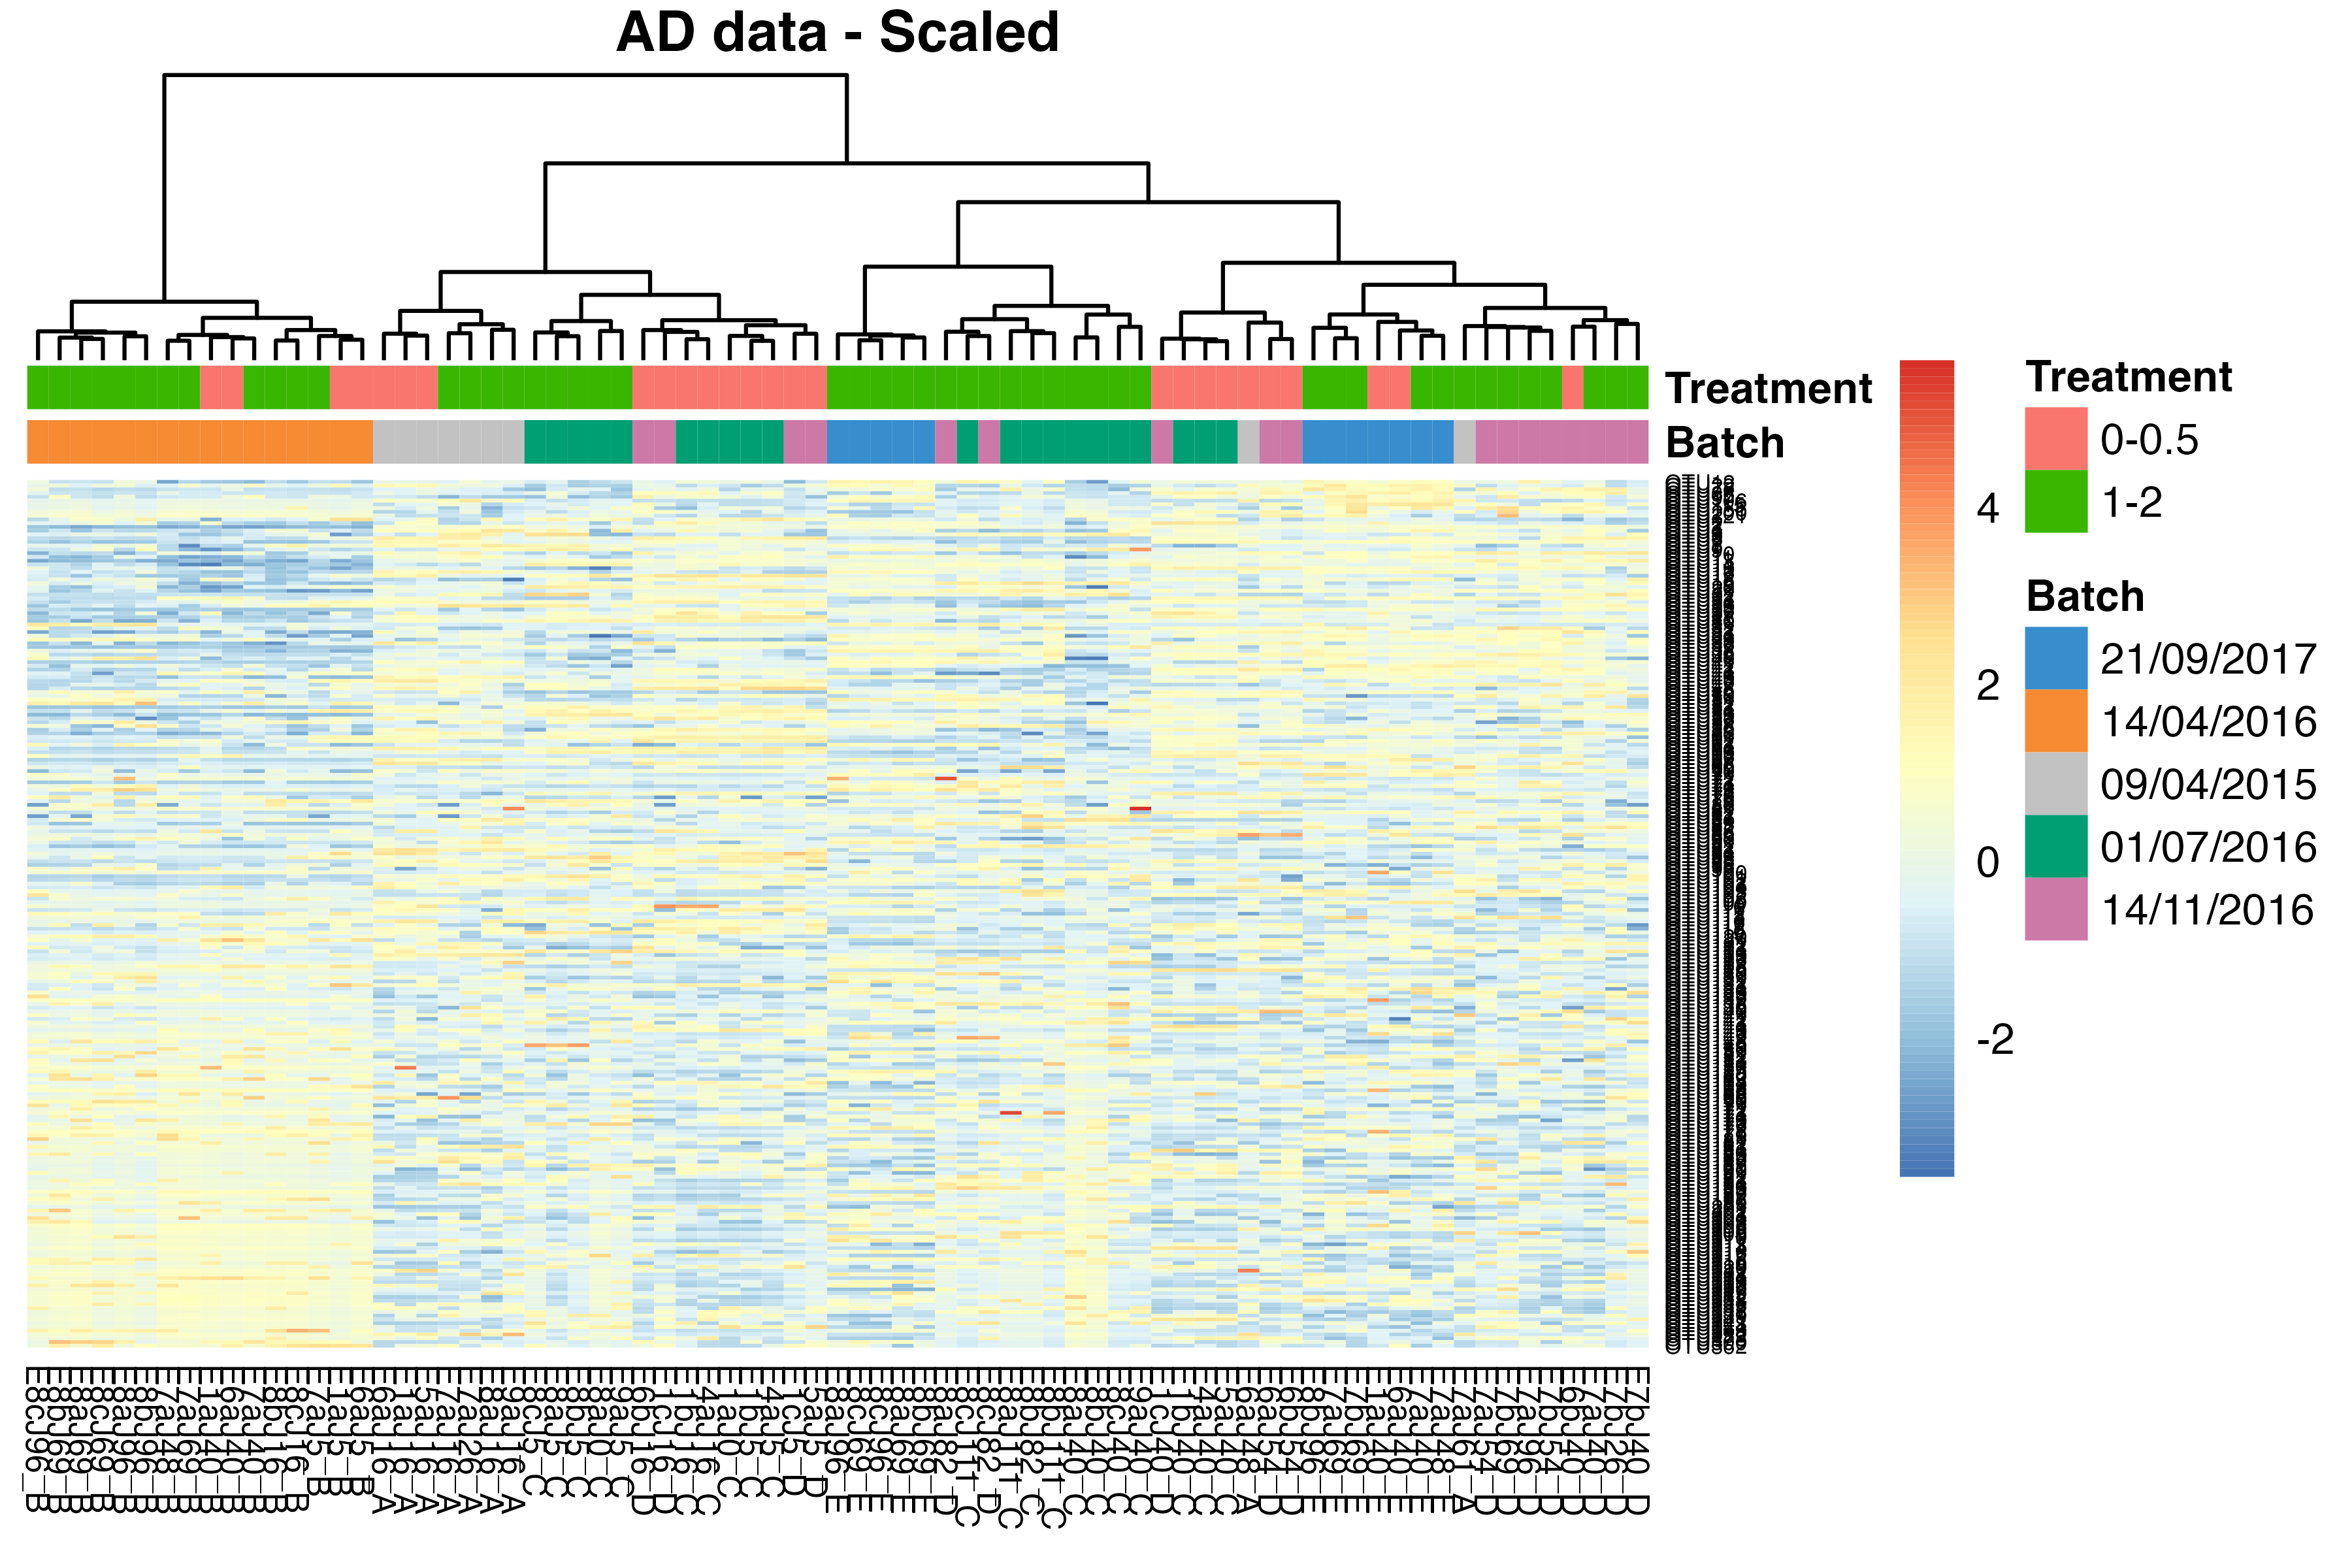
\includegraphics[width=0.9\linewidth]{PLSDAbatch_workflow_files/figure-latex/ADheatmap-1} 

}

\caption{Hierarchical clustering for samples in the AD data.}\label{fig:ADheatmap}
\end{figure}

In the heatmap, samples in the \textcolor{blue}{AD data} from batch dated ``14/04/2016'' were clustered and distinct from other samples, indicating a batch effect.

\hypertarget{prda}{%
\subsection{pRDA}\label{prda}}

We apply pRDA with \texttt{varpart()} function from \textcolor{orange}{vegan} R package.

\begin{Shaded}
\begin{Highlighting}[]
\CommentTok{\# AD data}
\NormalTok{ad.factors.df }\OtherTok{\textless{}{-}} \FunctionTok{data.frame}\NormalTok{(}\AttributeTok{trt =}\NormalTok{ ad.trt, }\AttributeTok{batch =}\NormalTok{ ad.batch)}
\FunctionTok{class}\NormalTok{(ad.clr) }\OtherTok{\textless{}{-}} \StringTok{\textquotesingle{}matrix\textquotesingle{}}
\NormalTok{ad.rda.before }\OtherTok{\textless{}{-}} \FunctionTok{varpart}\NormalTok{(ad.clr, }\SpecialCharTok{\textasciitilde{}}\NormalTok{ trt, }\SpecialCharTok{\textasciitilde{}}\NormalTok{ batch, }
                         \AttributeTok{data =}\NormalTok{ ad.factors.df, }\AttributeTok{scale =} \ConstantTok{TRUE}\NormalTok{)}
\NormalTok{ad.rda.before}\SpecialCharTok{$}\NormalTok{part}\SpecialCharTok{$}\NormalTok{indfract}
\end{Highlighting}
\end{Shaded}

\begin{verbatim}
##                 Df R.squared Adj.R.squared Testable
## [a] = X1|X2      1        NA    0.08943682     TRUE
## [b] = X2|X1      4        NA    0.26604420     TRUE
## [c]              0        NA    0.01296248    FALSE
## [d] = Residuals NA        NA    0.63155651    FALSE
\end{verbatim}

In the result, \texttt{X1} and \texttt{X2} represent the first and second covariates fitted in the model. \texttt{{[}a{]}}, \texttt{{[}b{]}} represent the independent proportion of variance explained by \texttt{X1} and \texttt{X2} respectively, and \texttt{{[}c{]}} represents the intersection variance shared between \texttt{X1} and \texttt{X2}. In the \textcolor{blue}{AD data}, batch variance (\texttt{X2}) was larger than treatment variance (\texttt{X1}) with some interaction proportion (indicated in line \texttt{{[}c{]}}, Adj.R.squared = 0.013). The greater the intersection variance, the more unbalanced batch x treatment design is. In this study, we considered the design as approx. balanced.

\begin{Shaded}
\begin{Highlighting}[]
\CommentTok{\# Sponge data}
\NormalTok{sponge.batch }\OtherTok{\textless{}{-}}\NormalTok{ sponge\_data}\SpecialCharTok{$}\NormalTok{Y.bat}
\NormalTok{sponge.trt }\OtherTok{\textless{}{-}}\NormalTok{ sponge\_data}\SpecialCharTok{$}\NormalTok{Y.trt}

\NormalTok{sponge.factors.df }\OtherTok{\textless{}{-}} \FunctionTok{data.frame}\NormalTok{(}\AttributeTok{trt =}\NormalTok{ sponge.trt, }\AttributeTok{batch =}\NormalTok{ sponge.batch)}
\FunctionTok{class}\NormalTok{(sponge.clr) }\OtherTok{\textless{}{-}} \StringTok{\textquotesingle{}matrix\textquotesingle{}}
\NormalTok{sponge.rda.before }\OtherTok{\textless{}{-}} \FunctionTok{varpart}\NormalTok{(sponge.clr, }\SpecialCharTok{\textasciitilde{}}\NormalTok{ trt, }\SpecialCharTok{\textasciitilde{}}\NormalTok{ batch, }
                             \AttributeTok{data =}\NormalTok{ sponge.factors.df, }\AttributeTok{scale =} \ConstantTok{TRUE}\NormalTok{)}
\NormalTok{sponge.rda.before}\SpecialCharTok{$}\NormalTok{part}\SpecialCharTok{$}\NormalTok{indfract}
\end{Highlighting}
\end{Shaded}

\begin{verbatim}
##                 Df R.squared Adj.R.squared Testable
## [a] = X1|X2      1        NA    0.16572246     TRUE
## [b] = X2|X1      1        NA    0.16396277     TRUE
## [c]              0        NA   -0.01063501    FALSE
## [d] = Residuals NA        NA    0.68094977    FALSE
\end{verbatim}

The \textcolor{brown}{sponge data} have a completely balanced batch x treatment design, so there was no intersection variance (indicated in line \texttt{{[}c{]}}, Adj.R.squared = -0.01) detected. The proportion of treatment and batch variance is nearly equal as indicated in lines \texttt{{[}a{]}} and \texttt{{[}b{]}}.

\begin{Shaded}
\begin{Highlighting}[]
\CommentTok{\# HD data}
\FunctionTok{data}\NormalTok{(}\StringTok{\textquotesingle{}HD\_data\textquotesingle{}}\NormalTok{)}
\NormalTok{hd.clr }\OtherTok{\textless{}{-}}\NormalTok{ HD\_data}\SpecialCharTok{$}\NormalTok{EgData}\SpecialCharTok{$}\NormalTok{X.clr}
\NormalTok{hd.trt }\OtherTok{\textless{}{-}}\NormalTok{ HD\_data}\SpecialCharTok{$}\NormalTok{EgData}\SpecialCharTok{$}\NormalTok{Y.trt}
\NormalTok{hd.batch }\OtherTok{\textless{}{-}}\NormalTok{ HD\_data}\SpecialCharTok{$}\NormalTok{EgData}\SpecialCharTok{$}\NormalTok{Y.bat}

\NormalTok{hd.factors.df }\OtherTok{\textless{}{-}} \FunctionTok{data.frame}\NormalTok{(}\AttributeTok{trt =}\NormalTok{ hd.trt, }\AttributeTok{batch =}\NormalTok{ hd.batch)}
\FunctionTok{class}\NormalTok{(hd.clr) }\OtherTok{\textless{}{-}} \StringTok{\textquotesingle{}matrix\textquotesingle{}}
\NormalTok{hd.rda.before }\OtherTok{\textless{}{-}} \FunctionTok{varpart}\NormalTok{(hd.clr, }\SpecialCharTok{\textasciitilde{}}\NormalTok{ trt, }\SpecialCharTok{\textasciitilde{}}\NormalTok{ batch, }
                         \AttributeTok{data =}\NormalTok{ hd.factors.df, }\AttributeTok{scale =} \ConstantTok{TRUE}\NormalTok{)}
\NormalTok{hd.rda.before}\SpecialCharTok{$}\NormalTok{part}\SpecialCharTok{$}\NormalTok{indfract}
\end{Highlighting}
\end{Shaded}

\begin{verbatim}
##                 Df R.squared Adj.R.squared Testable
## [a] = X1|X2      0        NA -2.220446e-16    FALSE
## [b] = X2|X1      8        NA  1.608205e-01     TRUE
## [c]              0        NA  9.730583e-02    FALSE
## [d] = Residuals NA        NA  7.418737e-01    FALSE
\end{verbatim}

Collinearity was detected in the \textcolor{violet}{HD data} between treatment and batch as indicated by lines \texttt{{[}a{]}} (Adj.R.squared = 0) and \texttt{{[}c{]}} (Adj.R.squared = 0.097) that all treatment variance was explained as intersection variance, because the batch x treatment design is nested. The intersection variance in such a design is usually considerable. As the intersection is shared between batch and treatment effects, the batch variance in the \textcolor{violet}{HD data} was larger than the treatment variance.

\hypertarget{managing-batch-effects}{%
\section{Managing batch effects}\label{managing-batch-effects}}

\hypertarget{accnt}{%
\subsection{Accounting for batch effects}\label{accnt}}

The methods that we use to account for batch effects include the methods designed for microbiome data: zero-inflated Gaussian (ZIG) mixture model and the methods adapted for microbiome data: linear regression, SVA and RUV4. Among them, SVA and RUV4 were designed for unknown batch effects.

\hypertarget{methods-designed-for-microbiome-data}{%
\subsubsection{Methods designed for microbiome data}\label{methods-designed-for-microbiome-data}}

\textbf{Zero-inflated Gaussian mixture model} To use the ZIG model, we first create a \texttt{MRexperiment} object applying \texttt{newMRexperiment()} (from \textcolor{orange}{metagenomeSeq} package) to microbiome counts and annotated data frames with metadata and taxonomic information generated with \texttt{AnnotatedDataFrame()} from \textcolor{orange}{Biobase} package.

\begin{Shaded}
\begin{Highlighting}[]
\CommentTok{\# Creating a MRexperiment object (make sure no NA in metadata)}
\NormalTok{AD.phenotypeData }\OtherTok{=} \FunctionTok{AnnotatedDataFrame}\NormalTok{(}\AttributeTok{data =}\NormalTok{ AD\_data}\SpecialCharTok{$}\NormalTok{FullData}\SpecialCharTok{$}\NormalTok{metadata)}
\NormalTok{AD.taxaData }\OtherTok{=} \FunctionTok{AnnotatedDataFrame}\NormalTok{(}\AttributeTok{data =}\NormalTok{ AD\_data}\SpecialCharTok{$}\NormalTok{FullData}\SpecialCharTok{$}\NormalTok{taxa)}
\NormalTok{AD.obj }\OtherTok{=} \FunctionTok{newMRexperiment}\NormalTok{(}\AttributeTok{counts =} \FunctionTok{t}\NormalTok{(AD\_data}\SpecialCharTok{$}\NormalTok{FullData}\SpecialCharTok{$}\NormalTok{X.count), }
                         \AttributeTok{phenoData =}\NormalTok{ AD.phenotypeData, }
                         \AttributeTok{featureData =}\NormalTok{ AD.taxaData)}
\NormalTok{AD.obj}
\end{Highlighting}
\end{Shaded}

\begin{verbatim}
## MRexperiment (storageMode: environment)
## assayData: 567 features, 75 samples 
##   element names: counts 
## protocolData: none
## phenoData
##   sampleNames: E1aJ16_A E5aJ16_A ... E8cJ96_E (75 total)
##   varLabels: sample_name.data.extraction analysis_name ...
##     initial_phenol_concentration.regroup (7 total)
##   varMetadata: labelDescription
## featureData
##   featureNames: OTU12 OTU29 ... OTU17710 (567 total)
##   fvarLabels: Kingdom Phylum ... Species (7 total)
##   fvarMetadata: labelDescription
## experimentData: use 'experimentData(object)'
## Annotation:
\end{verbatim}

The \textcolor{blue}{AD count data} are then filtered with \texttt{filterData()} function (from \textcolor{orange}{metagenomeSeq}). We can use \texttt{MRcounts()} to extract the count data from the \texttt{MRexperiment} object.

\begin{Shaded}
\begin{Highlighting}[]
\CommentTok{\# filtering data to maintain a threshold of minimum depth or OTU presence}
\FunctionTok{dim}\NormalTok{(}\FunctionTok{MRcounts}\NormalTok{(AD.obj))}
\end{Highlighting}
\end{Shaded}

\begin{verbatim}
## [1] 567  75
\end{verbatim}

\begin{Shaded}
\begin{Highlighting}[]
\NormalTok{AD.obj }\OtherTok{=} \FunctionTok{filterData}\NormalTok{(}\AttributeTok{obj =}\NormalTok{ AD.obj, }\AttributeTok{present =} \DecValTok{20}\NormalTok{, }\AttributeTok{depth =} \DecValTok{5}\NormalTok{)}
\FunctionTok{dim}\NormalTok{(}\FunctionTok{MRcounts}\NormalTok{(AD.obj))}
\end{Highlighting}
\end{Shaded}

\begin{verbatim}
## [1] 289  75
\end{verbatim}

After filtering, the \textcolor{blue}{AD count data} were reduced to 289 OTUs and 75 samples.

We calculate the percentile for CSS normalisation with \texttt{cumNormStatFast()} function (from \textcolor{orange}{metagenomeSeq} package). The CSS normalisation is applied with \texttt{cumNorm()} and the normalised data can be exported using \texttt{MRcounts()} with \texttt{norm\ =\ TRUE}. The normalisation scaling factors for each sample, which are the sum of counts up to the calculated percentile, can be accessed through \texttt{normFactors()}. We calculate the log transfomed scaling factors by diving them with their median, which are better than the default scaling factors that are divided by 1000 (\texttt{log2(normFactors(obj)/1000\ +\ 1)}).

\begin{Shaded}
\begin{Highlighting}[]
\CommentTok{\# calculate the percentile for CSS normalisation}
\NormalTok{AD.pctl }\OtherTok{=} \FunctionTok{cumNormStatFast}\NormalTok{(}\AttributeTok{obj =}\NormalTok{ AD.obj)}
\CommentTok{\# CSS normalisation}
\NormalTok{AD.obj }\OtherTok{\textless{}{-}} \FunctionTok{cumNorm}\NormalTok{(}\AttributeTok{obj =}\NormalTok{ AD.obj, }\AttributeTok{p =}\NormalTok{ AD.pctl)}
\CommentTok{\# export normalised data}
\NormalTok{AD.norm.data }\OtherTok{\textless{}{-}} \FunctionTok{MRcounts}\NormalTok{(}\AttributeTok{obj =}\NormalTok{ AD.obj, }\AttributeTok{norm =} \ConstantTok{TRUE}\NormalTok{)}

\CommentTok{\# normalisation scaling factors for each sample }
\NormalTok{AD.normFactor }\OtherTok{=} \FunctionTok{normFactors}\NormalTok{(}\AttributeTok{object =}\NormalTok{ AD.obj)}
\NormalTok{AD.normFactor }\OtherTok{=} \FunctionTok{log2}\NormalTok{(AD.normFactor}\SpecialCharTok{/}\FunctionTok{median}\NormalTok{(AD.normFactor) }\SpecialCharTok{+} \DecValTok{1}\NormalTok{)}
\end{Highlighting}
\end{Shaded}

We create a design matrix with treatment variable (\texttt{phenol\_conc}), batch variable (\texttt{seq\_run}) and the log transformed scaling factors using \texttt{model.matrix()}, and then apply the ZIG model by \texttt{fitZig()} function. We set \texttt{useCSSoffset\ =\ FALSE} to avoid using the default scaling factors as we have already included our customised scaling factor (\texttt{AD.normFactor}) in the design matrix.

\begin{Shaded}
\begin{Highlighting}[]
\CommentTok{\# treatment variable}
\NormalTok{phenol\_conc }\OtherTok{=} \FunctionTok{pData}\NormalTok{(}\AttributeTok{object =}\NormalTok{ AD.obj)}\SpecialCharTok{$}\NormalTok{initial\_phenol\_concentration.regroup}
\CommentTok{\# batch variable}
\NormalTok{seq\_run }\OtherTok{=} \FunctionTok{pData}\NormalTok{(}\AttributeTok{object =}\NormalTok{ AD.obj)}\SpecialCharTok{$}\NormalTok{sequencing\_run\_date}

\CommentTok{\# build a design matrix}
\NormalTok{AD.mod.full }\OtherTok{=} \FunctionTok{model.matrix}\NormalTok{(}\SpecialCharTok{\textasciitilde{}}\NormalTok{ phenol\_conc }\SpecialCharTok{+}\NormalTok{ seq\_run }\SpecialCharTok{+}\NormalTok{ AD.normFactor)}

\CommentTok{\# settings for the fitZig() function}
\NormalTok{AD.settings }\OtherTok{\textless{}{-}} \FunctionTok{zigControl}\NormalTok{(}\AttributeTok{maxit =} \DecValTok{10}\NormalTok{, }\AttributeTok{verbose =} \ConstantTok{TRUE}\NormalTok{)}

\CommentTok{\# apply the ZIG model}
\NormalTok{ADfit }\OtherTok{\textless{}{-}} \FunctionTok{fitZig}\NormalTok{(}\AttributeTok{obj =}\NormalTok{ AD.obj, }\AttributeTok{mod =}\NormalTok{ AD.mod.full, }
                \AttributeTok{useCSSoffset =} \ConstantTok{FALSE}\NormalTok{, }\AttributeTok{control =}\NormalTok{ AD.settings)}
\end{Highlighting}
\end{Shaded}

\begin{verbatim}
## it= 0, nll=123.44, log10(eps+1)=Inf, stillActive=289
## it= 1, nll=134.33, log10(eps+1)=0.04, stillActive=10
## it= 2, nll=134.64, log10(eps+1)=0.01, stillActive=1
## it= 3, nll=134.80, log10(eps+1)=0.00, stillActive=0
\end{verbatim}

The OTUs with the top 50 smallest p values are extracted using \texttt{MRcoefs()}. We set \texttt{eff\ =\ 0.5}, so only the OTUs with at least ``0.5'' quantile (50\%) number of effective samples (positive samples + estimated undersampling zeroes) are extracted.

\begin{Shaded}
\begin{Highlighting}[]
\NormalTok{ADcoefs }\OtherTok{\textless{}{-}} \FunctionTok{MRcoefs}\NormalTok{(ADfit, }\AttributeTok{coef =} \DecValTok{2}\NormalTok{, }\AttributeTok{group =} \DecValTok{3}\NormalTok{, }\AttributeTok{number =} \DecValTok{50}\NormalTok{, }\AttributeTok{eff =} \FloatTok{0.5}\NormalTok{)}
\FunctionTok{head}\NormalTok{(ADcoefs)}
\end{Highlighting}
\end{Shaded}

\begin{verbatim}
##       phenol_conc1-2      pvalues   adjPvalues
## OTU68      -2.901041 2.467451e-15 4.081959e-13
## OTU46      -2.847212 2.824885e-15 4.081959e-13
## OTU28      -2.449290 4.012023e-14 3.864915e-12
## OTU24      -2.846452 6.397959e-14 4.622526e-12
## OTU59      -1.815250 3.784889e-13 2.187666e-11
## OTU65      -2.141183 3.342621e-11 1.610029e-09
\end{verbatim}

\hypertarget{other-methods-adapted-for-microbiome-data}{%
\subsubsection{Other methods adapted for microbiome data}\label{other-methods-adapted-for-microbiome-data}}

\textbf{Linear regression} Linear regression is conducted with \texttt{linear\_regres()} function in \textcolor{orange}{PLSDAbatch}. We integrated the \textcolor{orange}{performance} package that assesses performance of regression models into our function \texttt{linear\_regres()}. Therefore, we can apply \texttt{check\_model()} from \textcolor{orange}{performance} to the outputs from \texttt{linear\_regres()} to diagnose the validity of the model fitted with treatment and batch effects for each variable \citep{daniel2020performance}. We can extract performance measurements such as adjusted R2, RMSE, RSE, AIC and BIC for the models fitted with and without batch effects, which are also the outputs of \texttt{linear\_regres()}.

We apply \texttt{type\ =\ "linear\ model"} to the \textcolor{blue}{AD data} because of the balanced batch x treatment design.

\begin{Shaded}
\begin{Highlighting}[]
\CommentTok{\# AD data}
\NormalTok{ad.clr }\OtherTok{\textless{}{-}}\NormalTok{ ad.clr[}\FunctionTok{seq\_len}\NormalTok{(}\FunctionTok{nrow}\NormalTok{(ad.clr)), }\FunctionTok{seq\_len}\NormalTok{(}\FunctionTok{ncol}\NormalTok{(ad.clr))]}
\NormalTok{ad.lm }\OtherTok{\textless{}{-}} \FunctionTok{linear\_regres}\NormalTok{(}\AttributeTok{data =}\NormalTok{ ad.clr, }\AttributeTok{trt =}\NormalTok{ ad.trt, }
                       \AttributeTok{batch.fix =}\NormalTok{ ad.batch, }\AttributeTok{type =} \StringTok{\textquotesingle{}linear model\textquotesingle{}}\NormalTok{)}

\NormalTok{ad.p }\OtherTok{\textless{}{-}} \FunctionTok{sapply}\NormalTok{(ad.lm}\SpecialCharTok{$}\NormalTok{lm.table, }\ControlFlowTok{function}\NormalTok{(x)\{x}\SpecialCharTok{$}\NormalTok{coefficients[}\DecValTok{2}\NormalTok{,}\DecValTok{4}\NormalTok{]\})}
\NormalTok{ad.p.adj }\OtherTok{\textless{}{-}} \FunctionTok{p.adjust}\NormalTok{(}\AttributeTok{p =}\NormalTok{ ad.p, }\AttributeTok{method =} \StringTok{\textquotesingle{}fdr\textquotesingle{}}\NormalTok{)}

\FunctionTok{check\_model}\NormalTok{(ad.lm}\SpecialCharTok{$}\NormalTok{model}\SpecialCharTok{$}\NormalTok{OTU12)}
\end{Highlighting}
\end{Shaded}

\begin{figure}

{\centering \includegraphics[width=1\linewidth]{PLSDAbatch_workflow_files/figure-latex/ADlm-1} 

}

\caption{Diagnostic plots for the model fitted with batch effects of "OTU12" in the AD data.}\label{fig:ADlm}
\end{figure}

To diagnose the validity of the model fitted with both treatment and batch effects, we use different plots to check the assumptions of each microbial variable. For example, the diagnostic plots of ``OTU12'' are shown in the above figure panel. The simulated data under the fitted model were close to the real data (shown as green line), indicating good model fitness (top panel). The linearity (or homoscedasticity) and homogeneity of variance were not satisfied. The correlation between batch (\texttt{batch.fix}) and treatment (\texttt{trt}) effects was very low, indicating a good model with low collinearity. Some samples could be classified as outliers with a Cook's distance larger than or equal to 0.5, for example, ``57'', ``39'', ``47'', ``44'' and ``16'' (middle panel). The distribution of residuals was very close to normal (bottom panel). For the microbial variables with some assumptions not met, we should be careful about their results.

For performance measurements of models fitted with or without batch effects, We show an example of the results for some variables.

\begin{Shaded}
\begin{Highlighting}[]
\FunctionTok{head}\NormalTok{(ad.lm}\SpecialCharTok{$}\NormalTok{adj.R2)}
\end{Highlighting}
\end{Shaded}

\begin{verbatim}
##            trt.only trt.batch
## OTU12   0.008445545 0.4785532
## OTU29  -0.012966020 0.7808945
## OTU77  -0.013343146 0.4779754
## OTU86   0.183743803 0.2850153
## OTU97  -0.008989284 0.4502563
## OTU106  0.072963581 0.8745676
\end{verbatim}

The adjusted \(R^2\) of the model with both treatment and batch effects for all the OTUs listed was larger than the model with treatment effects only, suggesting that the model fitted with batch effects explained more data variance, and was thus better than the model without batch effects.

We next look at the AIC of models fitted with or without batch effects.

\begin{Shaded}
\begin{Highlighting}[]
\FunctionTok{head}\NormalTok{(ad.lm}\SpecialCharTok{$}\NormalTok{AIC)}
\end{Highlighting}
\end{Shaded}

\begin{verbatim}
##        trt.only trt.batch
## OTU12  208.5626 164.13617
## OTU29  266.0485 154.99072
## OTU77  180.7800 134.80638
## OTU86  212.2987 206.13722
## OTU97  161.6715 119.90108
## OTU106 205.4135  59.17005
\end{verbatim}

A lower AIC indicates a better fit, here for a model fitted with batch effects for all the OTUs.

Both results strongly indicated that a batch effect should be fitted in the linear model.

We apply a \texttt{"linear\ mixed\ model"} to the \textcolor{violet}{HD data} because of the nested batch x treatment design.

\begin{Shaded}
\begin{Highlighting}[]
\CommentTok{\# HD data}
\NormalTok{hd.lmm }\OtherTok{\textless{}{-}} \FunctionTok{linear\_regres}\NormalTok{(}\AttributeTok{data =}\NormalTok{ hd.clr, }\AttributeTok{trt =}\NormalTok{ hd.trt, }
                        \AttributeTok{batch.random =}\NormalTok{ hd.batch, }
                        \AttributeTok{type =} \StringTok{\textquotesingle{}linear mixed model\textquotesingle{}}\NormalTok{)}
\end{Highlighting}
\end{Shaded}

\begin{Shaded}
\begin{Highlighting}[]
\NormalTok{hd.p }\OtherTok{\textless{}{-}} \FunctionTok{sapply}\NormalTok{(hd.lmm}\SpecialCharTok{$}\NormalTok{lmm.table, }\ControlFlowTok{function}\NormalTok{(x)\{x}\SpecialCharTok{$}\NormalTok{coefficients[}\DecValTok{2}\NormalTok{,}\DecValTok{5}\NormalTok{]\})}
\NormalTok{hd.p.adj }\OtherTok{\textless{}{-}} \FunctionTok{p.adjust}\NormalTok{(}\AttributeTok{p =}\NormalTok{ hd.p, }\AttributeTok{method =} \StringTok{\textquotesingle{}fdr\textquotesingle{}}\NormalTok{)}

\FunctionTok{check\_model}\NormalTok{(hd.lmm}\SpecialCharTok{$}\NormalTok{model}\SpecialCharTok{$}\NormalTok{OTU1)}
\end{Highlighting}
\end{Shaded}

\begin{figure}

{\centering \includegraphics[width=1\linewidth]{PLSDAbatch_workflow_files/figure-latex/HDlmm-1} 

}

\caption{Diagnostic plots for the model fitted with batch effects of "OTU1" in the HD data.}\label{fig:HDlmm}
\end{figure}

According to the diagnostic plots of ``OTU1'' as shown in the above figure panel, the simulated data under the fitted model were not very close to the real data (shown as green line), indicating an imperfect fitness (top panel). The linearity (or homoscedasticity) and homogeneity of variance were not satisfied. Some samples could be classified as outliers with a Cook's distance larger than or equal to 0.5, for example, ``12'', ``21'', ``20'', ``11'' and ``6'' (middle panel). The distribution of residuals was not normal, while the one of random effects was very close to normal (bottom panel).

We then look at the AIC of models fitted with or without batch effects.

\begin{Shaded}
\begin{Highlighting}[]
\FunctionTok{head}\NormalTok{(hd.lmm}\SpecialCharTok{$}\NormalTok{AIC)}
\end{Highlighting}
\end{Shaded}

\begin{verbatim}
##       trt.only trt.batch
## OTU1  60.00637  65.46410
## OTU2 130.14167 130.96344
## OTU3  71.76985  75.58915
## OTU4 134.59992 134.04812
## OTU5 150.25059 148.30644
## OTU6  99.92864  99.05391
\end{verbatim}

For some OTUs, the model fitted without batch effects was better with a lower AIC, e.g., ``OTU1'', ``OTU2'' and ``OTU3''. ``OTU4'', ``OTU5'' and ``OTU6'' were more appropriate within a model with batch effects.

Since we apply a \texttt{"linear\ mixed\ model"} to the \textcolor{violet}{HD data}, this type of model can only output conditional \(R^2\) that includes the variance of both fixed and random effects (treatment, fixed and random batch effects) and marginal \(R^2\) that includes only the variance of fixed effects (treatment and fixed batch effects) \citep{nakagawa2013general}. The marginal \(R^2\)s of the models with and without the batch effect in the \textcolor{violet}{HD data} should be the same theoretically, as marginal \(R^2\) only includes fixed effects and the treatment effect was the only fixed effect here. In the actual calculation, the results of these two models were not the same, because part of the variance was explained by the random effect in the model fitted with the batch effect.

\begin{Shaded}
\begin{Highlighting}[]
\FunctionTok{head}\NormalTok{(hd.lmm}\SpecialCharTok{$}\NormalTok{cond.R2)}
\end{Highlighting}
\end{Shaded}

\begin{verbatim}
##        trt.only trt.batch
## OTU1 0.47917775 0.5161317
## OTU2 0.39223824 0.4729848
## OTU3 0.02091376 0.2636432
## OTU4 0.37200835 0.5672392
## OTU5 0.07858373 0.2938212
## OTU6 0.41388250 0.6143134
\end{verbatim}

\begin{Shaded}
\begin{Highlighting}[]
\FunctionTok{head}\NormalTok{(hd.lmm}\SpecialCharTok{$}\NormalTok{marg.R2)}
\end{Highlighting}
\end{Shaded}

\begin{verbatim}
##        trt.only  trt.batch
## OTU1 0.47917775 0.46735273
## OTU2 0.39223824 0.38459672
## OTU3 0.02091376 0.01489608
## OTU4 0.37200835 0.36122754
## OTU5 0.07858373 0.06052938
## OTU6 0.41388250 0.40749149
\end{verbatim}

We observed that some variables resulted in singular fits (\texttt{error\ message:\ Can\textquotesingle{}t\ compute\ random\ effect\ variances.\ Some\ variance\ components\ equal\ zero.\ Your\ model\ may\ suffer\ from\ singulariy.}), which are expected to happen in linear mixed models when covariates are nested. We recommend noting the variables for which this error occurs, as it may lead to unreliable results.

\textbf{SVA} accounts for unknown batch effects. Here we assume that the batch grouping information in the \textcolor{blue}{AD data} is unknown. We first build two design matrices with (\texttt{ad.mod}) and without (\texttt{ad.mod0}) treatment grouping information generated with \texttt{model.matrix()} function from \textcolor{orange}{stats}. We then use \texttt{num.sv()} from \textcolor{orange}{sva} package to determine the number of batch variables \texttt{n.sv} that is used to estimate batch effects in function \texttt{sva()}.

\begin{Shaded}
\begin{Highlighting}[]
\CommentTok{\# estimate batch effects}
\NormalTok{ad.mod }\OtherTok{\textless{}{-}} \FunctionTok{model.matrix}\NormalTok{( }\SpecialCharTok{\textasciitilde{}}\NormalTok{ ad.trt)}
\NormalTok{ad.mod0 }\OtherTok{\textless{}{-}} \FunctionTok{model.matrix}\NormalTok{( }\SpecialCharTok{\textasciitilde{}} \DecValTok{1}\NormalTok{, }\AttributeTok{data =}\NormalTok{ ad.trt)}
\NormalTok{ad.sva.n }\OtherTok{\textless{}{-}} \FunctionTok{num.sv}\NormalTok{(}\AttributeTok{dat =} \FunctionTok{t}\NormalTok{(ad.clr), }\AttributeTok{mod =}\NormalTok{ ad.mod, }\AttributeTok{method =} \StringTok{\textquotesingle{}leek\textquotesingle{}}\NormalTok{)}
\NormalTok{ad.sva }\OtherTok{\textless{}{-}} \FunctionTok{sva}\NormalTok{(}\FunctionTok{t}\NormalTok{(ad.clr), ad.mod, ad.mod0, }\AttributeTok{n.sv =}\NormalTok{ ad.sva.n)}
\end{Highlighting}
\end{Shaded}

\begin{verbatim}
## Number of significant surrogate variables is:  4 
## Iteration (out of 5 ):1  2  3  4  5
\end{verbatim}

The estimated batch effects are then applied to \texttt{f.pvalue()} to calculate the P-values of treatment effects. The estimated batch effects in SVA are assumed to be independent of the treatment effects. However, SVA considers some correlation between batch and treatment effects \citep{wang2020managing}.

\begin{Shaded}
\begin{Highlighting}[]
\CommentTok{\# include estimated batch effects in the linear model}
\NormalTok{ad.mod.batch }\OtherTok{\textless{}{-}} \FunctionTok{cbind}\NormalTok{(ad.mod, ad.sva}\SpecialCharTok{$}\NormalTok{sv)}
\NormalTok{ad.mod0.batch }\OtherTok{\textless{}{-}} \FunctionTok{cbind}\NormalTok{(ad.mod0, ad.sva}\SpecialCharTok{$}\NormalTok{sv)}
\NormalTok{ad.sva.p }\OtherTok{\textless{}{-}} \FunctionTok{f.pvalue}\NormalTok{(}\FunctionTok{t}\NormalTok{(ad.clr), ad.mod.batch, ad.mod0.batch)}
\NormalTok{ad.sva.p.adj }\OtherTok{\textless{}{-}} \FunctionTok{p.adjust}\NormalTok{(ad.sva.p, }\AttributeTok{method =} \StringTok{\textquotesingle{}fdr\textquotesingle{}}\NormalTok{)}
\end{Highlighting}
\end{Shaded}

\textbf{RUV4} Before applying RUV4 (\texttt{RUV4()} from \textcolor{orange}{ruv} package), we need to specify negative control variables and the number of batch variables to estimate. We can use the empirical negative controls that are not significantly differentially abundant (adjusted P \textgreater{} 0.05) from a linear regression with the treatment information as the only covariate.

We use a loop to fit a linear regression for each microbial variable and adjust P values of treatment effects for multiple comparisons with \texttt{p.adjust()} from \textcolor{orange}{stats}. The empirical negative controls are then extracted according to the adjusted P values.

\begin{Shaded}
\begin{Highlighting}[]
\CommentTok{\# empirical negative controls}
\NormalTok{ad.empir.p }\OtherTok{\textless{}{-}} \FunctionTok{c}\NormalTok{()}
\ControlFlowTok{for}\NormalTok{(e }\ControlFlowTok{in} \FunctionTok{seq\_len}\NormalTok{(}\FunctionTok{ncol}\NormalTok{(ad.clr)))\{}
\NormalTok{  ad.empir.lm }\OtherTok{\textless{}{-}} \FunctionTok{lm}\NormalTok{(ad.clr[,e] }\SpecialCharTok{\textasciitilde{}}\NormalTok{ ad.trt)}
\NormalTok{  ad.empir.p[e] }\OtherTok{\textless{}{-}} \FunctionTok{summary}\NormalTok{(ad.empir.lm)}\SpecialCharTok{$}\NormalTok{coefficients[}\DecValTok{2}\NormalTok{,}\DecValTok{4}\NormalTok{]}
\NormalTok{\}}
\NormalTok{ad.empir.p.adj }\OtherTok{\textless{}{-}} \FunctionTok{p.adjust}\NormalTok{(}\AttributeTok{p =}\NormalTok{ ad.empir.p, }\AttributeTok{method =} \StringTok{\textquotesingle{}fdr\textquotesingle{}}\NormalTok{)}
\NormalTok{ad.nc }\OtherTok{\textless{}{-}}\NormalTok{ ad.empir.p.adj }\SpecialCharTok{\textgreater{}} \FloatTok{0.05}
\end{Highlighting}
\end{Shaded}

The number of batch variables \texttt{k} can be determined using \texttt{getK()} function.

\begin{Shaded}
\begin{Highlighting}[]
\CommentTok{\# estimate k}
\NormalTok{ad.k.res }\OtherTok{\textless{}{-}} \FunctionTok{getK}\NormalTok{(}\AttributeTok{Y =}\NormalTok{ ad.clr, }\AttributeTok{X =}\NormalTok{ ad.trt, }\AttributeTok{ctl =}\NormalTok{ ad.nc)}
\NormalTok{ad.k }\OtherTok{\textless{}{-}}\NormalTok{ ad.k.res}\SpecialCharTok{$}\NormalTok{k}
\end{Highlighting}
\end{Shaded}

We then apply \texttt{RUV4()} with known treatment variables, estimated negative control variables and \texttt{k} batch variables. The calculated P values also need to be adjusted for multiple comparisons.

\begin{Shaded}
\begin{Highlighting}[]
\CommentTok{\# RUV4}
\NormalTok{ad.ruv4 }\OtherTok{\textless{}{-}} \FunctionTok{RUV4}\NormalTok{(}\AttributeTok{Y =}\NormalTok{ ad.clr, }\AttributeTok{X =}\NormalTok{ ad.trt, }\AttributeTok{ctl =}\NormalTok{ ad.nc, }\AttributeTok{k =}\NormalTok{ ad.k) }
\NormalTok{ad.ruv4.p }\OtherTok{\textless{}{-}}\NormalTok{ ad.ruv4}\SpecialCharTok{$}\NormalTok{p}
\NormalTok{ad.ruv4.p.adj }\OtherTok{\textless{}{-}} \FunctionTok{p.adjust}\NormalTok{(ad.ruv4.p, }\AttributeTok{method =} \StringTok{"fdr"}\NormalTok{)}
\end{Highlighting}
\end{Shaded}

Note: A package named \textcolor{orange}{RUVSeq} has been developed for count data. It provides \texttt{RUVg()} using negative control variables, and also other functions \texttt{RUVs()} and \texttt{RUVr()} using sample replicates \citep{moskovicz2020skin} or residuals from the regression on treatment effects to estimate and then account for latent batch effects. However, for CLR-transformed data, we still recommend the standard \textcolor{orange}{ruv} package.

\hypertarget{corrct}{%
\subsection{Correcting for batch effects}\label{corrct}}

The methods that we use to correct for batch effects include removeBatchEffect, ComBat, PLSDA-batch, sPLSDA-batch, Percentile Normalisation and RUVIII. Among them, RUVIII was designed for unknown batch effects. They were all applied to and illustrated with the \textcolor{blue}{AD data}.

\textbf{removeBatchEffect}

The \texttt{removeBatchEffect()} function is implemented in \textcolor{orange}{limma} package. The design matrix (\texttt{design}) with treatment grouping information can be generated with \texttt{model.matrix()} function from \textcolor{orange}{stats} as shown in section \textbf{accounting for batch effects} method ``SVA''.

Here we use \texttt{removeBatchEffect()} function with batch grouping information (\texttt{batch}) and treatment design matrix (\texttt{design}) to calculate batch effect corrected data \texttt{ad.rBE}.

\begin{Shaded}
\begin{Highlighting}[]
\NormalTok{ad.rBE }\OtherTok{\textless{}{-}} \FunctionTok{t}\NormalTok{(}\FunctionTok{removeBatchEffect}\NormalTok{(}\FunctionTok{t}\NormalTok{(ad.clr), }\AttributeTok{batch =}\NormalTok{ ad.batch, }
                              \AttributeTok{design =}\NormalTok{ ad.mod))}
\end{Highlighting}
\end{Shaded}

\textbf{ComBat}

The \texttt{ComBat()} function (from \textcolor{orange}{sva} package) is implemented as parametric or non-parametric correction with option \texttt{par.prior}. Under a parametric adjustment, we can assess the model's validity with \texttt{prior.plots\ =\ T} \citep{leek2012sva}.

Here we use a non-parametric correction (\texttt{par.prior\ =\ FALSE}) with batch grouping information (\texttt{batch}) and treatment design matrix (\texttt{mod}) to calculate batch effect corrected data \texttt{ad.ComBat}.

\begin{Shaded}
\begin{Highlighting}[]
\NormalTok{ad.ComBat }\OtherTok{\textless{}{-}} \FunctionTok{t}\NormalTok{(}\FunctionTok{ComBat}\NormalTok{(}\FunctionTok{t}\NormalTok{(ad.clr), }\AttributeTok{batch =}\NormalTok{ ad.batch, }
                      \AttributeTok{mod =}\NormalTok{ ad.mod, }\AttributeTok{par.prior =} \ConstantTok{FALSE}\NormalTok{))}
\end{Highlighting}
\end{Shaded}

\textbf{PLSDA-batch}

The \texttt{PLSDA\_batch()} function is implemented in \textcolor{orange}{PLSDAbatch} package. To use this function, we need to specify the optimal number of components related to treatment (\texttt{ncomp.trt}) or batch effects (\texttt{ncomp.bat}).

Here in the \textcolor{blue}{AD data}, we use \texttt{plsda()} from \textcolor{orange}{mixOmics} with only treatment grouping information to estimate the optimal number of treatment components to preserve.

\begin{Shaded}
\begin{Highlighting}[]
\CommentTok{\# estimate the number of treatment components}
\NormalTok{ad.trt.tune }\OtherTok{\textless{}{-}} \FunctionTok{plsda}\NormalTok{(}\AttributeTok{X =}\NormalTok{ ad.clr, }\AttributeTok{Y =}\NormalTok{ ad.trt, }\AttributeTok{ncomp =} \DecValTok{5}\NormalTok{)}
\NormalTok{ad.trt.tune}\SpecialCharTok{$}\NormalTok{prop\_expl\_var }\CommentTok{\#1}
\end{Highlighting}
\end{Shaded}

\begin{verbatim}
## $X
##      comp1      comp2      comp3      comp4      comp5 
## 0.18619506 0.07873817 0.08257396 0.09263497 0.06594757 
## 
## $Y
##      comp1      comp2      comp3      comp4      comp5 
## 1.00000000 0.33857374 0.17315267 0.10551296 0.08185822
\end{verbatim}

We choose the number that explains 100\% variance in the outcome matrix \texttt{Y}, thus from the result, 1 component was enough to preserve the treatment information.

We then use \texttt{PLSDA\_batch()} function with both treatment and batch grouping information to estimate the optimal number of batch components to remove.

\begin{Shaded}
\begin{Highlighting}[]
\CommentTok{\# estimate the number of batch components}
\NormalTok{ad.batch.tune }\OtherTok{\textless{}{-}} \FunctionTok{PLSDA\_batch}\NormalTok{(}\AttributeTok{X =}\NormalTok{ ad.clr, }
                             \AttributeTok{Y.trt =}\NormalTok{ ad.trt, }\AttributeTok{Y.bat =}\NormalTok{ ad.batch,}
                             \AttributeTok{ncomp.trt =} \DecValTok{1}\NormalTok{, }\AttributeTok{ncomp.bat =} \DecValTok{10}\NormalTok{)}
\NormalTok{ad.batch.tune}\SpecialCharTok{$}\NormalTok{explained\_variance.bat }\CommentTok{\#4}
\end{Highlighting}
\end{Shaded}

\begin{verbatim}
## $X
##      comp1      comp2      comp3      comp4      comp5      comp6      comp7 
## 0.17470922 0.11481264 0.10122717 0.07507395 0.03946605 0.03399731 0.03784224 
##      comp8      comp9     comp10 
## 0.02313026 0.02395840 0.01389336 
## 
## $Y
##       comp1       comp2       comp3       comp4       comp5       comp6 
## 0.247465374 0.261574081 0.230138238 0.260822307 0.230056326 0.246345583 
##       comp7       comp8       comp9      comp10 
## 0.267963500 0.252208822 0.003425768 0.240095146
\end{verbatim}

\begin{Shaded}
\begin{Highlighting}[]
\FunctionTok{sum}\NormalTok{(ad.batch.tune}\SpecialCharTok{$}\NormalTok{explained\_variance.bat}\SpecialCharTok{$}\NormalTok{Y[}\FunctionTok{seq\_len}\NormalTok{(}\DecValTok{4}\NormalTok{)])}
\end{Highlighting}
\end{Shaded}

\begin{verbatim}
## [1] 1
\end{verbatim}

Using the same criterion as choosing treatment components, we choose the number of batch components that explains 100\% variance in the outcome matrix of batch. According to the result, 4 components were required to remove batch effects.

We then can correct for batch effects applying \texttt{PLSDA\_batch()} with treatment, batch grouping information and corresponding optimal number of related components.

\begin{Shaded}
\begin{Highlighting}[]
\NormalTok{ad.PLSDA\_batch.res }\OtherTok{\textless{}{-}} \FunctionTok{PLSDA\_batch}\NormalTok{(}\AttributeTok{X =}\NormalTok{ ad.clr, }
                                  \AttributeTok{Y.trt =}\NormalTok{ ad.trt, }\AttributeTok{Y.bat =}\NormalTok{ ad.batch,}
                                  \AttributeTok{ncomp.trt =} \DecValTok{1}\NormalTok{, }\AttributeTok{ncomp.bat =} \DecValTok{4}\NormalTok{)}
\NormalTok{ad.PLSDA\_batch }\OtherTok{\textless{}{-}}\NormalTok{ ad.PLSDA\_batch.res}\SpecialCharTok{$}\NormalTok{X.nobatch}
\end{Highlighting}
\end{Shaded}

\textbf{sPLSDA-batch}

We apply sPLSDA-batch using the same function \texttt{PLSDA\_batch()}, but we specify the number of variables to select on each component (usually only treatment-related components \texttt{keepX.trt}). To determine the optimal number of variables to select, we use \texttt{tune.splsda()} function from \textcolor{orange}{mixOmics} package \citep{rohart2017mixomics} with all possible numbers of variables to select for each component (\texttt{test.keepX}).

\begin{Shaded}
\begin{Highlighting}[]
\CommentTok{\# estimate the number of variables to select per treatment component}
\FunctionTok{set.seed}\NormalTok{(}\DecValTok{777}\NormalTok{)}
\NormalTok{ad.test.keepX }\OtherTok{=} \FunctionTok{c}\NormalTok{(}\FunctionTok{seq}\NormalTok{(}\DecValTok{1}\NormalTok{, }\DecValTok{10}\NormalTok{, }\DecValTok{1}\NormalTok{), }\FunctionTok{seq}\NormalTok{(}\DecValTok{20}\NormalTok{, }\DecValTok{100}\NormalTok{, }\DecValTok{10}\NormalTok{), }
                  \FunctionTok{seq}\NormalTok{(}\DecValTok{150}\NormalTok{, }\DecValTok{231}\NormalTok{, }\DecValTok{50}\NormalTok{), }\DecValTok{231}\NormalTok{)}
\NormalTok{ad.trt.tune.v }\OtherTok{\textless{}{-}} \FunctionTok{tune.splsda}\NormalTok{(}\AttributeTok{X =}\NormalTok{ ad.clr, }\AttributeTok{Y =}\NormalTok{ ad.trt, }
                             \AttributeTok{ncomp =} \DecValTok{1}\NormalTok{, }\AttributeTok{test.keepX =}\NormalTok{ ad.test.keepX, }
                             \AttributeTok{validation =} \StringTok{\textquotesingle{}Mfold\textquotesingle{}}\NormalTok{, }\AttributeTok{folds =} \DecValTok{4}\NormalTok{, }
                             \AttributeTok{nrepeat =} \DecValTok{50}\NormalTok{)}
\NormalTok{ad.trt.tune.v}\SpecialCharTok{$}\NormalTok{choice.keepX }\CommentTok{\#100}
\end{Highlighting}
\end{Shaded}

Here the optimal number of variables to select for the treatment component was 100. Since we have adjusted the amount of treatment variation to preserve, we need to re-choose the optimal number of components related to batch effects using the same criterion mentioned in section \textbf{correcting for batch effects} method ``PLSDA-batch''.

\begin{Shaded}
\begin{Highlighting}[]
\CommentTok{\# estimate the number of batch components}
\NormalTok{ad.batch.tune }\OtherTok{\textless{}{-}} \FunctionTok{PLSDA\_batch}\NormalTok{(}\AttributeTok{X =}\NormalTok{ ad.clr, }
                             \AttributeTok{Y.trt =}\NormalTok{ ad.trt, }\AttributeTok{Y.bat =}\NormalTok{ ad.batch,}
                             \AttributeTok{ncomp.trt =} \DecValTok{1}\NormalTok{, }\AttributeTok{keepX.trt =} \DecValTok{100}\NormalTok{,}
                             \AttributeTok{ncomp.bat =} \DecValTok{10}\NormalTok{)}
\NormalTok{ad.batch.tune}\SpecialCharTok{$}\NormalTok{explained\_variance.bat }\CommentTok{\#4}
\end{Highlighting}
\end{Shaded}

\begin{verbatim}
## $X
##      comp1      comp2      comp3      comp4      comp5      comp6      comp7 
## 0.17420018 0.11477097 0.09813477 0.07894965 0.02946813 0.03702255 0.03195744 
##      comp8      comp9     comp10 
## 0.04098959 0.01559967 0.01584227 
## 
## $Y
##      comp1      comp2      comp3      comp4      comp5      comp6      comp7 
## 0.24747749 0.26067155 0.23010809 0.26174286 0.26062893 0.26282635 0.24125867 
##      comp8      comp9     comp10 
## 0.22162763 0.01365842 0.25965197
\end{verbatim}

\begin{Shaded}
\begin{Highlighting}[]
\FunctionTok{sum}\NormalTok{(ad.batch.tune}\SpecialCharTok{$}\NormalTok{explained\_variance.bat}\SpecialCharTok{$}\NormalTok{Y[}\FunctionTok{seq\_len}\NormalTok{(}\DecValTok{4}\NormalTok{)])}
\end{Highlighting}
\end{Shaded}

\begin{verbatim}
## [1] 1
\end{verbatim}

According to the result, we needed 4 batch related components to remove batch variance from the data with function \texttt{PLSDA\_batch()}.

\begin{Shaded}
\begin{Highlighting}[]
\NormalTok{ad.sPLSDA\_batch.res }\OtherTok{\textless{}{-}} \FunctionTok{PLSDA\_batch}\NormalTok{(}\AttributeTok{X =}\NormalTok{ ad.clr, }
                                   \AttributeTok{Y.trt =}\NormalTok{ ad.trt, }\AttributeTok{Y.bat =}\NormalTok{ ad.batch,}
                                   \AttributeTok{ncomp.trt =} \DecValTok{1}\NormalTok{, }\AttributeTok{keepX.trt =} \DecValTok{100}\NormalTok{,}
                                   \AttributeTok{ncomp.bat =} \DecValTok{4}\NormalTok{)}
\NormalTok{ad.sPLSDA\_batch }\OtherTok{\textless{}{-}}\NormalTok{ ad.sPLSDA\_batch.res}\SpecialCharTok{$}\NormalTok{X.nobatch}
\end{Highlighting}
\end{Shaded}

Note: for unbalanced batch x treatment design (with the exception of the nested design), we can specify \texttt{balance\ =\ FALSE} in \texttt{PLSDA\_batch()} function to apply weighted PLSDA-batch.

\textbf{Percentile Normalisation}

To apply \texttt{percentile\_norm()} function from \textcolor{orange}{PLSDAbatch} package, we need to indicate a control group (\texttt{ctrl.grp}).

\begin{Shaded}
\begin{Highlighting}[]
\NormalTok{ad.PN }\OtherTok{\textless{}{-}} \FunctionTok{percentile\_norm}\NormalTok{(}\AttributeTok{data =}\NormalTok{ ad.clr, }\AttributeTok{batch =}\NormalTok{ ad.batch, }
                         \AttributeTok{trt =}\NormalTok{ ad.trt, }\AttributeTok{ctrl.grp =} \StringTok{\textquotesingle{}0{-}0.5\textquotesingle{}}\NormalTok{)}
\end{Highlighting}
\end{Shaded}

\textbf{RUVIII}

The \texttt{RUVIII()} function is from \textcolor{orange}{ruv} package. Similar to \texttt{RUV4()}, we use empirical negative control variables and \texttt{getK()} to determine the number of batch variables (\texttt{k}) to estimate. We also need sample replicates which should be structured into a mapping matrix using \texttt{replicate.matrix()}. We can then obtain the batch effect corrected data applying \texttt{RUVIII()} with above elements.

\begin{Shaded}
\begin{Highlighting}[]
\NormalTok{ad.replicates }\OtherTok{\textless{}{-}}\NormalTok{ ad.metadata}\SpecialCharTok{$}\NormalTok{sample\_name.data.extraction}
\NormalTok{ad.replicates.matrix }\OtherTok{\textless{}{-}} \FunctionTok{replicate.matrix}\NormalTok{(ad.replicates)}

\NormalTok{ad.RUVIII }\OtherTok{\textless{}{-}} \FunctionTok{RUVIII}\NormalTok{(}\AttributeTok{Y =}\NormalTok{ ad.clr, }\AttributeTok{M =}\NormalTok{ ad.replicates.matrix, }
                    \AttributeTok{ctl =}\NormalTok{ ad.nc, }\AttributeTok{k =}\NormalTok{ ad.k)}
\FunctionTok{rownames}\NormalTok{(ad.RUVIII) }\OtherTok{\textless{}{-}} \FunctionTok{rownames}\NormalTok{(ad.clr)}
\end{Highlighting}
\end{Shaded}

\hypertarget{assessing-batch-effect-correction}{%
\section{Assessing batch effect correction}\label{assessing-batch-effect-correction}}

We apply different visualisation and quantitative methods to assessing batch effect correction.

\hypertarget{methods-that-detect-batch-effects}{%
\subsection{Methods that detect batch effects}\label{methods-that-detect-batch-effects}}

\textbf{PCA}

In the \textcolor{blue}{AD data}, we compared the PCA sample plots before and after batch effect correction with different methods.

\begin{Shaded}
\begin{Highlighting}[]
\NormalTok{ad.pca.before }\OtherTok{\textless{}{-}} \FunctionTok{pca}\NormalTok{(ad.clr, }\AttributeTok{ncomp =} \DecValTok{3}\NormalTok{, }\AttributeTok{scale =} \ConstantTok{TRUE}\NormalTok{)}
\NormalTok{ad.pca.rBE }\OtherTok{\textless{}{-}} \FunctionTok{pca}\NormalTok{(ad.rBE, }\AttributeTok{ncomp =} \DecValTok{3}\NormalTok{, }\AttributeTok{scale =} \ConstantTok{TRUE}\NormalTok{)}
\NormalTok{ad.pca.ComBat }\OtherTok{\textless{}{-}} \FunctionTok{pca}\NormalTok{(ad.ComBat, }\AttributeTok{ncomp =} \DecValTok{3}\NormalTok{, }\AttributeTok{scale =} \ConstantTok{TRUE}\NormalTok{)}
\NormalTok{ad.pca.PLSDA\_batch }\OtherTok{\textless{}{-}} \FunctionTok{pca}\NormalTok{(ad.PLSDA\_batch, }\AttributeTok{ncomp =} \DecValTok{3}\NormalTok{, }\AttributeTok{scale =} \ConstantTok{TRUE}\NormalTok{)}
\NormalTok{ad.pca.sPLSDA\_batch }\OtherTok{\textless{}{-}} \FunctionTok{pca}\NormalTok{(ad.sPLSDA\_batch, }\AttributeTok{ncomp =} \DecValTok{3}\NormalTok{, }\AttributeTok{scale =} \ConstantTok{TRUE}\NormalTok{)}
\NormalTok{ad.pca.PN }\OtherTok{\textless{}{-}} \FunctionTok{pca}\NormalTok{(ad.PN, }\AttributeTok{ncomp =} \DecValTok{3}\NormalTok{, }\AttributeTok{scale =} \ConstantTok{TRUE}\NormalTok{)}
\NormalTok{ad.pca.RUVIII }\OtherTok{\textless{}{-}} \FunctionTok{pca}\NormalTok{(ad.RUVIII, }\AttributeTok{ncomp =} \DecValTok{3}\NormalTok{, }\AttributeTok{scale =} \ConstantTok{TRUE}\NormalTok{)}
\end{Highlighting}
\end{Shaded}

\begin{Shaded}
\begin{Highlighting}[]
\CommentTok{\# order batches}
\NormalTok{ad.batch }\OtherTok{=} \FunctionTok{factor}\NormalTok{(ad.metadata}\SpecialCharTok{$}\NormalTok{sequencing\_run\_date, }
                  \AttributeTok{levels =} \FunctionTok{unique}\NormalTok{(ad.metadata}\SpecialCharTok{$}\NormalTok{sequencing\_run\_date))}

\NormalTok{ad.pca.before.plot }\OtherTok{\textless{}{-}} \FunctionTok{Scatter\_Density}\NormalTok{(}\AttributeTok{object =}\NormalTok{ ad.pca.before, }
                                      \AttributeTok{batch =}\NormalTok{ ad.batch, }
                                      \AttributeTok{trt =}\NormalTok{ ad.trt, }
                                      \AttributeTok{title =} \StringTok{\textquotesingle{}Before correction\textquotesingle{}}\NormalTok{)}
\end{Highlighting}
\end{Shaded}

\begin{Shaded}
\begin{Highlighting}[]
\NormalTok{ad.pca.rBE.plot }\OtherTok{\textless{}{-}} \FunctionTok{Scatter\_Density}\NormalTok{(}\AttributeTok{object =}\NormalTok{ ad.pca.rBE, }
                                   \AttributeTok{batch =}\NormalTok{ ad.batch, }
                                   \AttributeTok{trt =}\NormalTok{ ad.trt, }
                                   \AttributeTok{title =} \StringTok{\textquotesingle{}removeBatchEffect\textquotesingle{}}\NormalTok{)}
\end{Highlighting}
\end{Shaded}

\begin{Shaded}
\begin{Highlighting}[]
\NormalTok{ad.pca.ComBat.plot }\OtherTok{\textless{}{-}} \FunctionTok{Scatter\_Density}\NormalTok{(}\AttributeTok{object =}\NormalTok{ ad.pca.ComBat, }
                                      \AttributeTok{batch =}\NormalTok{ ad.batch, }
                                      \AttributeTok{trt =}\NormalTok{ ad.trt, }
                                      \AttributeTok{title =} \StringTok{\textquotesingle{}ComBat\textquotesingle{}}\NormalTok{)}
\end{Highlighting}
\end{Shaded}

\begin{Shaded}
\begin{Highlighting}[]
\NormalTok{ad.pca.PLSDA\_batch.plot }\OtherTok{\textless{}{-}} \FunctionTok{Scatter\_Density}\NormalTok{(}\AttributeTok{object =}\NormalTok{ ad.pca.PLSDA\_batch, }
                                           \AttributeTok{batch =}\NormalTok{ ad.batch, }
                                           \AttributeTok{trt =}\NormalTok{ ad.trt, }
                                           \AttributeTok{title =} \StringTok{\textquotesingle{}PLSDA{-}batch\textquotesingle{}}\NormalTok{)}
\end{Highlighting}
\end{Shaded}

\begin{Shaded}
\begin{Highlighting}[]
\NormalTok{ad.pca.sPLSDA\_batch.plot }\OtherTok{\textless{}{-}} \FunctionTok{Scatter\_Density}\NormalTok{(}\AttributeTok{object =}\NormalTok{ ad.pca.sPLSDA\_batch, }
                                            \AttributeTok{batch =}\NormalTok{ ad.batch, }
                                            \AttributeTok{trt =}\NormalTok{ ad.trt, }
                                            \AttributeTok{title =} \StringTok{\textquotesingle{}sPLSDA{-}batch\textquotesingle{}}\NormalTok{)}
\end{Highlighting}
\end{Shaded}

\begin{Shaded}
\begin{Highlighting}[]
\NormalTok{ad.pca.PN.plot }\OtherTok{\textless{}{-}} \FunctionTok{Scatter\_Density}\NormalTok{(}\AttributeTok{object =}\NormalTok{ ad.pca.PN, }
                                  \AttributeTok{batch =}\NormalTok{ ad.batch, }
                                  \AttributeTok{trt =}\NormalTok{ ad.trt, }
                                  \AttributeTok{title =} \StringTok{\textquotesingle{}Percentile Normalisation\textquotesingle{}}\NormalTok{)}
\end{Highlighting}
\end{Shaded}

\begin{Shaded}
\begin{Highlighting}[]
\NormalTok{ad.pca.RUVIII.plot }\OtherTok{\textless{}{-}} \FunctionTok{Scatter\_Density}\NormalTok{(}\AttributeTok{object =}\NormalTok{ ad.pca.RUVIII, }
                                      \AttributeTok{batch =}\NormalTok{ ad.batch, }
                                      \AttributeTok{trt =}\NormalTok{ ad.trt, }
                                      \AttributeTok{title =} \StringTok{\textquotesingle{}RUVIII\textquotesingle{}}\NormalTok{)}
\end{Highlighting}
\end{Shaded}

\begin{figure}

{\centering 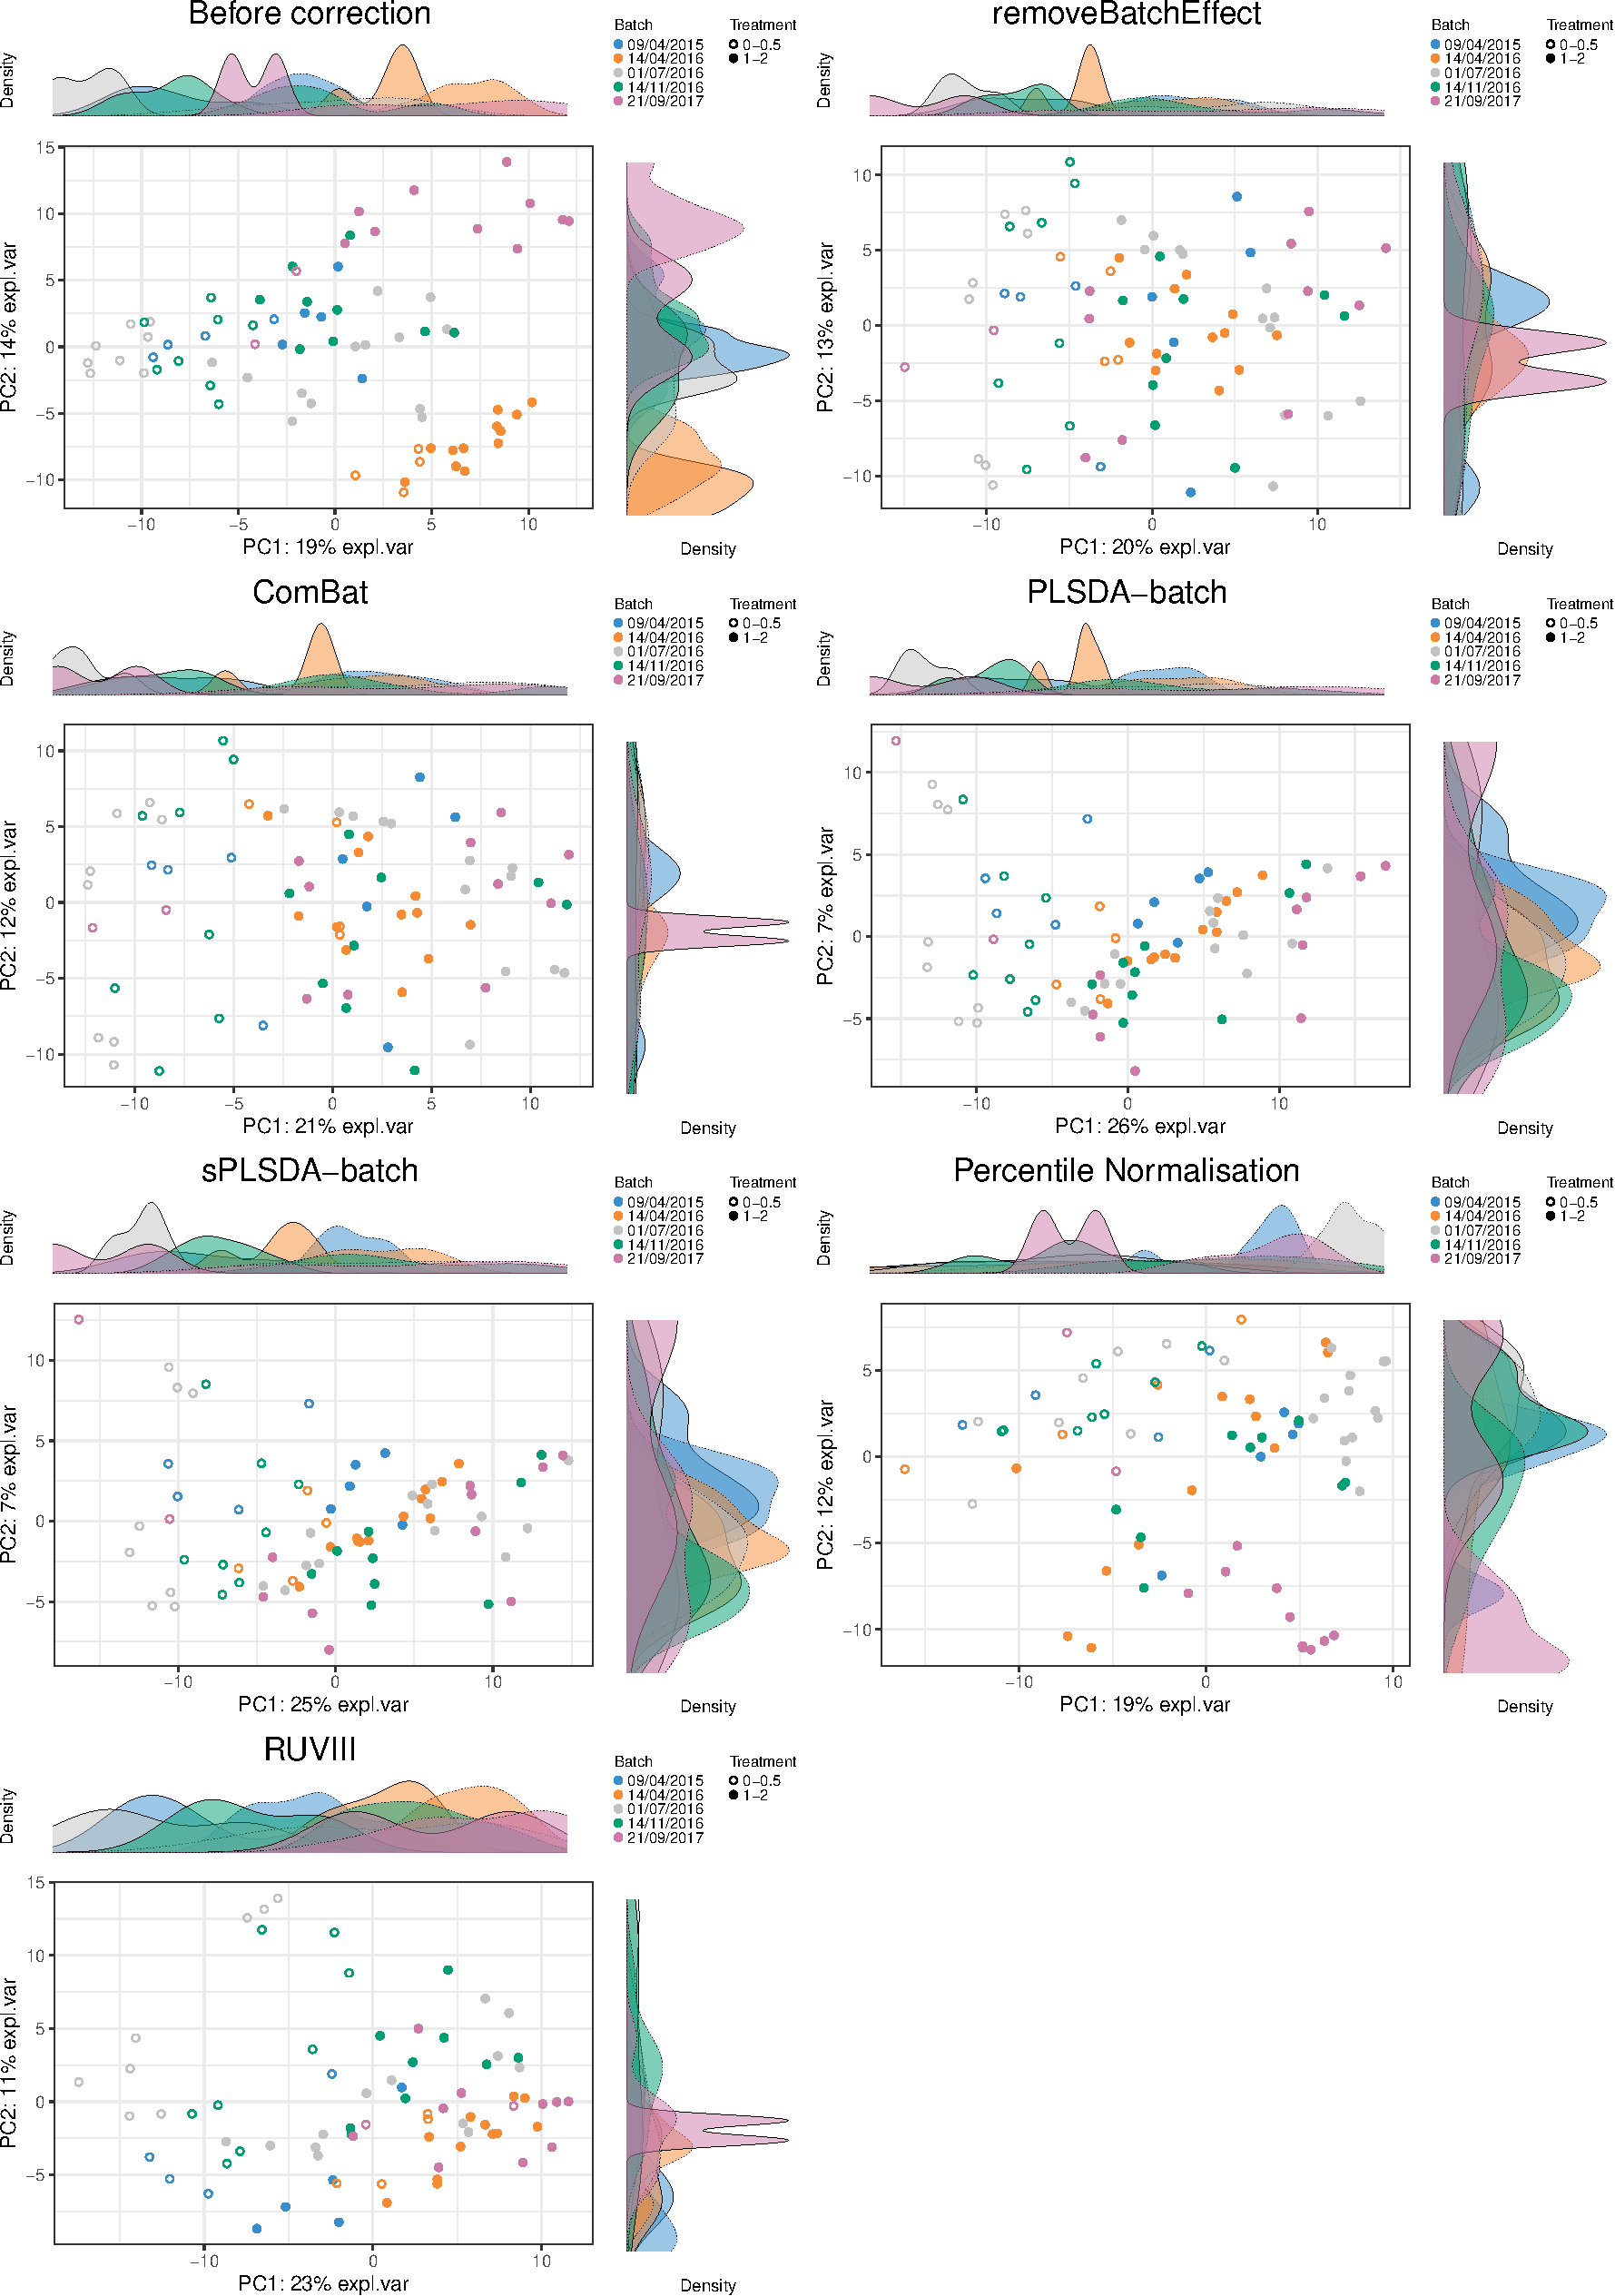
\includegraphics[width=1\linewidth]{PLSDAbatch_workflow_files/figure-latex/ADpca-1} 

}

\caption{The PCA sample plots with densities before and after batch effect correction in the AD data.}\label{fig:ADpca}
\end{figure}

As shown in the PCA sample plots, the differences between the samples sequenced at ``14/04/2016'', ``21/09/2017'' and the other dates were removed after batch effect correction with most methods except percentile normalisation. The data corrected with PLSDA-batch included more treatment variation mostly on the first PC than other method-corrected data, as indicated on the x-axis label (26\%). We can also compare the boxplots and density plots for key variables identified in PCA driving the major variance or heatmaps showing obvious patterns before and after batch effect correction (results not shown).

\textbf{pRDA}

We calculate the global explained variance across all microbial variables using pRDA. To achieve this, we create a loop for each variable from the original (uncorrected) and batch effect-corrected data. The final results are then displayed with \texttt{partVar\_plot()} from \textcolor{orange}{PLSDAbatch} package.

\begin{Shaded}
\begin{Highlighting}[]
\CommentTok{\# AD data}
\NormalTok{ad.corrected.list }\OtherTok{\textless{}{-}} \FunctionTok{list}\NormalTok{(}\StringTok{\textasciigrave{}}\AttributeTok{Before correction}\StringTok{\textasciigrave{}} \OtherTok{=}\NormalTok{ ad.clr, }
                          \AttributeTok{removeBatchEffect =}\NormalTok{ ad.rBE, }
                          \AttributeTok{ComBat =}\NormalTok{ ad.ComBat, }
                          \StringTok{\textasciigrave{}}\AttributeTok{PLSDA{-}batch}\StringTok{\textasciigrave{}} \OtherTok{=}\NormalTok{ ad.PLSDA\_batch, }
                          \StringTok{\textasciigrave{}}\AttributeTok{sPLSDA{-}batch}\StringTok{\textasciigrave{}} \OtherTok{=}\NormalTok{ ad.sPLSDA\_batch, }
                          \StringTok{\textasciigrave{}}\AttributeTok{Percentile Normalisation}\StringTok{\textasciigrave{}} \OtherTok{=}\NormalTok{ ad.PN,}
                          \AttributeTok{RUVIII =}\NormalTok{ ad.RUVIII)}

\NormalTok{ad.prop.df }\OtherTok{\textless{}{-}} \FunctionTok{data.frame}\NormalTok{(}\AttributeTok{Treatment =} \ConstantTok{NA}\NormalTok{, }\AttributeTok{Batch =} \ConstantTok{NA}\NormalTok{, }
                         \AttributeTok{Intersection =} \ConstantTok{NA}\NormalTok{, }
                         \AttributeTok{Residuals =} \ConstantTok{NA}\NormalTok{) }
\ControlFlowTok{for}\NormalTok{(i }\ControlFlowTok{in} \FunctionTok{seq\_len}\NormalTok{(}\FunctionTok{length}\NormalTok{(ad.corrected.list)))\{}
\NormalTok{  rda.res }\OtherTok{=} \FunctionTok{varpart}\NormalTok{(ad.corrected.list[[i]], }\SpecialCharTok{\textasciitilde{}}\NormalTok{ trt, }\SpecialCharTok{\textasciitilde{}}\NormalTok{ batch,}
                    \AttributeTok{data =}\NormalTok{ ad.factors.df, }\AttributeTok{scale =} \ConstantTok{TRUE}\NormalTok{)}
\NormalTok{  ad.prop.df[i, ] }\OtherTok{\textless{}{-}}\NormalTok{ rda.res}\SpecialCharTok{$}\NormalTok{part}\SpecialCharTok{$}\NormalTok{indfract}\SpecialCharTok{$}\NormalTok{Adj.R.squared\}}

\FunctionTok{rownames}\NormalTok{(ad.prop.df) }\OtherTok{=} \FunctionTok{names}\NormalTok{(ad.corrected.list)}

\NormalTok{ad.prop.df }\OtherTok{\textless{}{-}}\NormalTok{ ad.prop.df[, }\FunctionTok{c}\NormalTok{(}\DecValTok{1}\NormalTok{,}\DecValTok{3}\NormalTok{,}\DecValTok{2}\NormalTok{,}\DecValTok{4}\NormalTok{)]}

\NormalTok{ad.prop.df[ad.prop.df }\SpecialCharTok{\textless{}} \DecValTok{0}\NormalTok{] }\OtherTok{=} \DecValTok{0}
\NormalTok{ad.prop.df }\OtherTok{\textless{}{-}} \FunctionTok{as.data.frame}\NormalTok{(}\FunctionTok{t}\NormalTok{(}\FunctionTok{apply}\NormalTok{(ad.prop.df, }\DecValTok{1}\NormalTok{, }
                                    \ControlFlowTok{function}\NormalTok{(x)\{x}\SpecialCharTok{/}\FunctionTok{sum}\NormalTok{(x)\})))}

\FunctionTok{partVar\_plot}\NormalTok{(}\AttributeTok{prop.df =}\NormalTok{ ad.prop.df)}
\end{Highlighting}
\end{Shaded}

\begin{figure}

{\centering 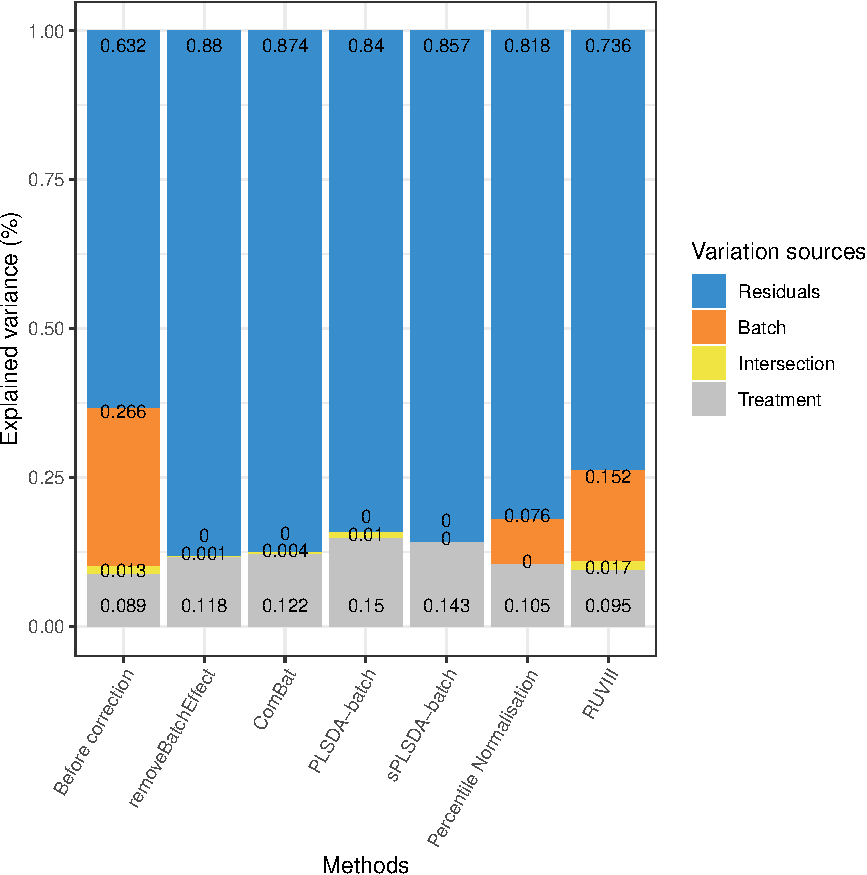
\includegraphics[width=0.6\linewidth]{PLSDAbatch_workflow_files/figure-latex/ADprda-1} 

}

\caption{Global explained variance before and after batch effect correction for the AD data.}\label{fig:ADprda}
\end{figure}

As shown in the above figure, the intersection between batch and treatment variance was small (1.3\%) for the \textcolor{blue}{AD data}, which implies that the batch x treatment design is not highly unbalanced. Thus the unweighted PLSDA-batch and sPLSDA-batch were still applicable, and thus the weighted versions were not used. sPLSDA-batch corrected data led to the best performance with a slightly higher proportion of treatment variance explained and undetectable batch and intersection variance compared to the other methods.

\begin{Shaded}
\begin{Highlighting}[]
\CommentTok{\# HFHS data}
\FunctionTok{data}\NormalTok{(}\StringTok{\textquotesingle{}HFHS\_data\textquotesingle{}}\NormalTok{)}
\NormalTok{hfhs.corrected.list }\OtherTok{\textless{}{-}}\NormalTok{ HFHS\_data}\SpecialCharTok{$}\NormalTok{CorrectData}\SpecialCharTok{$}\NormalTok{data}

\NormalTok{hfhs.trt }\OtherTok{\textless{}{-}}\NormalTok{ HFHS\_data}\SpecialCharTok{$}\NormalTok{CorrectData}\SpecialCharTok{$}\NormalTok{Y.trt}
\NormalTok{hfhs.batch }\OtherTok{\textless{}{-}}\NormalTok{ HFHS\_data}\SpecialCharTok{$}\NormalTok{CorrectData}\SpecialCharTok{$}\NormalTok{Y.bat}
\NormalTok{hfhs.factors.df }\OtherTok{\textless{}{-}} \FunctionTok{data.frame}\NormalTok{(}\AttributeTok{trt =}\NormalTok{ hfhs.trt, }\AttributeTok{batch =}\NormalTok{ hfhs.batch)}

\NormalTok{hfhs.prop.df }\OtherTok{\textless{}{-}} \FunctionTok{data.frame}\NormalTok{(}\AttributeTok{Treatment =} \ConstantTok{NA}\NormalTok{, }\AttributeTok{Batch =} \ConstantTok{NA}\NormalTok{, }
                           \AttributeTok{Intersection =} \ConstantTok{NA}\NormalTok{, }
                           \AttributeTok{Residuals =} \ConstantTok{NA}\NormalTok{) }
\ControlFlowTok{for}\NormalTok{(i }\ControlFlowTok{in} \FunctionTok{seq\_len}\NormalTok{(}\FunctionTok{length}\NormalTok{(hfhs.corrected.list)))\{}
\NormalTok{  rda.res }\OtherTok{=} \FunctionTok{varpart}\NormalTok{(hfhs.corrected.list[[i]], }\SpecialCharTok{\textasciitilde{}}\NormalTok{ trt, }\SpecialCharTok{\textasciitilde{}}\NormalTok{ batch,}
                    \AttributeTok{data =}\NormalTok{ hfhs.factors.df, }\AttributeTok{scale =} \ConstantTok{TRUE}\NormalTok{)}
\NormalTok{  hfhs.prop.df[i, ] }\OtherTok{\textless{}{-}}\NormalTok{ rda.res}\SpecialCharTok{$}\NormalTok{part}\SpecialCharTok{$}\NormalTok{indfract}\SpecialCharTok{$}\NormalTok{Adj.R.squared\}}

\FunctionTok{rownames}\NormalTok{(hfhs.prop.df) }\OtherTok{=} \FunctionTok{names}\NormalTok{(hfhs.corrected.list)}

\NormalTok{hfhs.prop.df }\OtherTok{\textless{}{-}}\NormalTok{ hfhs.prop.df[, }\FunctionTok{c}\NormalTok{(}\DecValTok{1}\NormalTok{,}\DecValTok{3}\NormalTok{,}\DecValTok{2}\NormalTok{,}\DecValTok{4}\NormalTok{)]}

\NormalTok{hfhs.prop.df[hfhs.prop.df }\SpecialCharTok{\textless{}} \DecValTok{0}\NormalTok{] }\OtherTok{=} \DecValTok{0}
\NormalTok{hfhs.prop.df }\OtherTok{\textless{}{-}} \FunctionTok{as.data.frame}\NormalTok{(}\FunctionTok{t}\NormalTok{(}\FunctionTok{apply}\NormalTok{(hfhs.prop.df, }\DecValTok{1}\NormalTok{, }
                                      \ControlFlowTok{function}\NormalTok{(x)\{x}\SpecialCharTok{/}\FunctionTok{sum}\NormalTok{(x)\})))}


\FunctionTok{partVar\_plot}\NormalTok{(}\AttributeTok{prop.df =}\NormalTok{ hfhs.prop.df)}
\end{Highlighting}
\end{Shaded}

\begin{figure}

{\centering 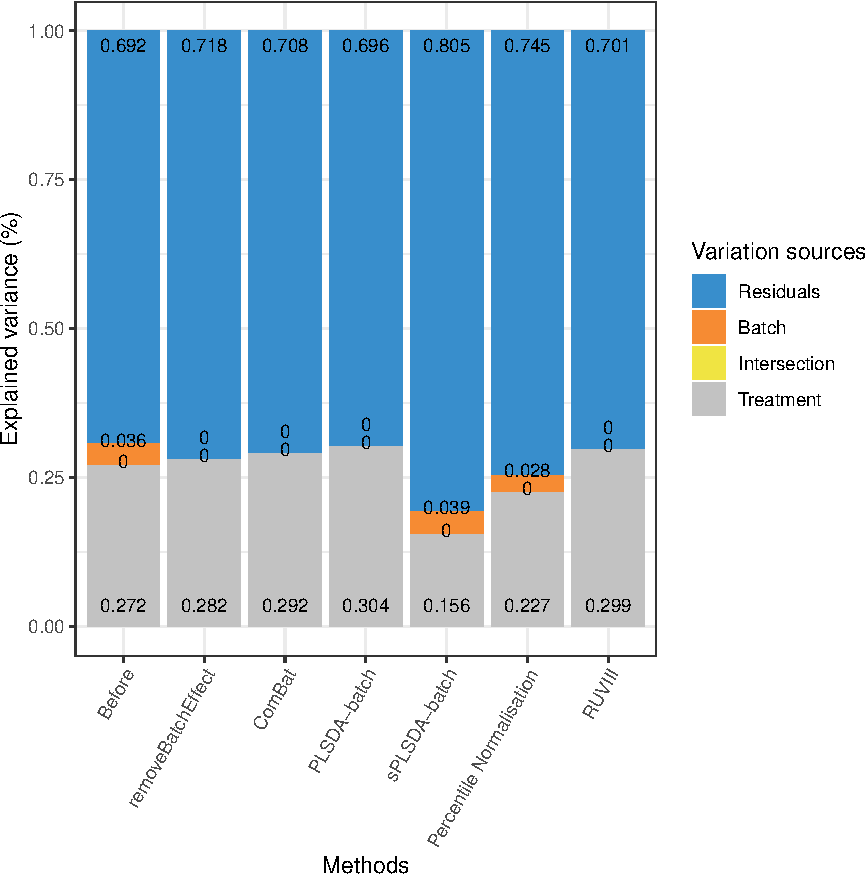
\includegraphics[width=0.6\linewidth]{PLSDAbatch_workflow_files/figure-latex/HFHSprda-1} 

}

\caption{Global explained variance before and after batch effect correction for the HFHS data.}\label{fig:HFHSprda}
\end{figure}

As shown in the above figure, a small amount of batch variance was observed (3.6\%) for the \textcolor{olive}{HFHS data}. PLSDA-batch achieved the best performance for preserving the largest treatment variance and completely removing batch variance compared to the other methods. The results also indicate that PLSDA-batch is more appropriate for weak batch effects, while sPLSDA-batch is more appropriate for strong batch effects. The RUVIII performed better in the \textcolor{olive}{HFHS data} than the \textcolor{blue}{AD data} because the sample replicates might capture more batch variation than in the \textcolor{blue}{AD data}. Indeed, the sample replicates in \textcolor{olive}{HFHS data} are across different day batches, while the replicates in \textcolor{blue}{AD data} do not exist in all batches. Therefore, sample replicates play a critical role in RUVIII.

\hypertarget{other-methods-1}{%
\subsection{Other methods}\label{other-methods-1}}

\(\mathbf{R^2}\)

The \(R^2\) values for each variable are calculated with \texttt{lm()} from \textcolor{orange}{stats} package. To compare the \(R^2\) values among variables, we scale the corrected data before \(R^2\) calculation. The results are displayed with \texttt{ggplot()} from \textcolor{orange}{ggplot2} R package.

\begin{Shaded}
\begin{Highlighting}[]
\CommentTok{\# AD data}
\CommentTok{\# scale}
\NormalTok{ad.corr\_scale.list }\OtherTok{\textless{}{-}} \FunctionTok{lapply}\NormalTok{(ad.corrected.list, }
                             \ControlFlowTok{function}\NormalTok{(x)\{}\FunctionTok{apply}\NormalTok{(x, }\DecValTok{2}\NormalTok{, scale)\})}

\NormalTok{ad.r\_values.list }\OtherTok{\textless{}{-}} \FunctionTok{list}\NormalTok{()}
\ControlFlowTok{for}\NormalTok{(i }\ControlFlowTok{in} \FunctionTok{seq\_len}\NormalTok{(}\FunctionTok{length}\NormalTok{(ad.corr\_scale.list)))\{}
\NormalTok{  ad.r\_values }\OtherTok{\textless{}{-}} \FunctionTok{data.frame}\NormalTok{(}\AttributeTok{trt =} \ConstantTok{NA}\NormalTok{, }\AttributeTok{batch =} \ConstantTok{NA}\NormalTok{)}
  \ControlFlowTok{for}\NormalTok{(c }\ControlFlowTok{in} \FunctionTok{seq\_len}\NormalTok{(}\FunctionTok{ncol}\NormalTok{(ad.corr\_scale.list[[i]])))\{}
\NormalTok{    ad.fit.res.trt }\OtherTok{\textless{}{-}} \FunctionTok{lm}\NormalTok{(ad.corr\_scale.list[[i]][,c] }\SpecialCharTok{\textasciitilde{}}\NormalTok{ ad.trt)}
\NormalTok{    ad.r\_values[c,}\DecValTok{1}\NormalTok{] }\OtherTok{\textless{}{-}} \FunctionTok{summary}\NormalTok{(ad.fit.res.trt)}\SpecialCharTok{$}\NormalTok{r.squared}
\NormalTok{    ad.fit.res.batch }\OtherTok{\textless{}{-}} \FunctionTok{lm}\NormalTok{(ad.corr\_scale.list[[i]][,c] }\SpecialCharTok{\textasciitilde{}}\NormalTok{ ad.batch)}
\NormalTok{    ad.r\_values[c,}\DecValTok{2}\NormalTok{] }\OtherTok{\textless{}{-}} \FunctionTok{summary}\NormalTok{(ad.fit.res.batch)}\SpecialCharTok{$}\NormalTok{r.squared}
\NormalTok{  \}}
\NormalTok{  ad.r\_values.list[[i]] }\OtherTok{\textless{}{-}}\NormalTok{ ad.r\_values}
\NormalTok{\}}
\FunctionTok{names}\NormalTok{(ad.r\_values.list) }\OtherTok{\textless{}{-}} \FunctionTok{names}\NormalTok{(ad.corr\_scale.list)}

\NormalTok{ad.boxp.list }\OtherTok{\textless{}{-}} \FunctionTok{list}\NormalTok{()}
\ControlFlowTok{for}\NormalTok{(i }\ControlFlowTok{in} \FunctionTok{seq\_len}\NormalTok{(}\FunctionTok{length}\NormalTok{(ad.r\_values.list)))\{}
\NormalTok{  ad.boxp.list[[i]] }\OtherTok{\textless{}{-}} 
    \FunctionTok{data.frame}\NormalTok{(}\AttributeTok{r2 =} \FunctionTok{c}\NormalTok{(ad.r\_values.list[[i]][ ,}\StringTok{\textquotesingle{}trt\textquotesingle{}}\NormalTok{],}
\NormalTok{                      ad.r\_values.list[[i]][ ,}\StringTok{\textquotesingle{}batch\textquotesingle{}}\NormalTok{]), }
               \AttributeTok{Effects =} \FunctionTok{as.factor}\NormalTok{(}\FunctionTok{rep}\NormalTok{(}\FunctionTok{c}\NormalTok{(}\StringTok{\textquotesingle{}Treatment\textquotesingle{}}\NormalTok{,}\StringTok{\textquotesingle{}Batch\textquotesingle{}}\NormalTok{), }
                                       \AttributeTok{each =} \DecValTok{231}\NormalTok{)))}
\NormalTok{\}}
\FunctionTok{names}\NormalTok{(ad.boxp.list) }\OtherTok{\textless{}{-}} \FunctionTok{names}\NormalTok{(ad.r\_values.list)}

\NormalTok{ad.r2.boxp }\OtherTok{\textless{}{-}} \FunctionTok{rbind}\NormalTok{(ad.boxp.list}\SpecialCharTok{$}\StringTok{\textasciigrave{}}\AttributeTok{Before correction}\StringTok{\textasciigrave{}}\NormalTok{,}
\NormalTok{                    ad.boxp.list}\SpecialCharTok{$}\NormalTok{removeBatchEffect,}
\NormalTok{                    ad.boxp.list}\SpecialCharTok{$}\NormalTok{ComBat,}
\NormalTok{                    ad.boxp.list}\SpecialCharTok{$}\StringTok{\textasciigrave{}}\AttributeTok{PLSDA{-}batch}\StringTok{\textasciigrave{}}\NormalTok{,}
\NormalTok{                    ad.boxp.list}\SpecialCharTok{$}\StringTok{\textasciigrave{}}\AttributeTok{sPLSDA{-}batch}\StringTok{\textasciigrave{}}\NormalTok{,}
\NormalTok{                    ad.boxp.list}\SpecialCharTok{$}\StringTok{\textasciigrave{}}\AttributeTok{Percentile Normalisation}\StringTok{\textasciigrave{}}\NormalTok{,}
\NormalTok{                    ad.boxp.list}\SpecialCharTok{$}\NormalTok{RUVIII)}

\NormalTok{ad.r2.boxp}\SpecialCharTok{$}\NormalTok{methods }\OtherTok{\textless{}{-}} \FunctionTok{rep}\NormalTok{(}\FunctionTok{c}\NormalTok{(}\StringTok{\textquotesingle{}Before correction\textquotesingle{}}\NormalTok{, }\StringTok{\textquotesingle{} removeBatchEffect\textquotesingle{}}\NormalTok{, }
                            \StringTok{\textquotesingle{}ComBat\textquotesingle{}}\NormalTok{,}\StringTok{\textquotesingle{}PLSDA{-}batch\textquotesingle{}}\NormalTok{, }\StringTok{\textquotesingle{}sPLSDA{-}batch\textquotesingle{}}\NormalTok{,}
                            \StringTok{\textquotesingle{}Percentile Normalisation\textquotesingle{}}\NormalTok{, }\StringTok{\textquotesingle{}RUVIII\textquotesingle{}}\NormalTok{), }\AttributeTok{each =} \DecValTok{462}\NormalTok{)}

\NormalTok{ad.r2.boxp}\SpecialCharTok{$}\NormalTok{methods }\OtherTok{\textless{}{-}} \FunctionTok{factor}\NormalTok{(ad.r2.boxp}\SpecialCharTok{$}\NormalTok{methods, }
                             \AttributeTok{levels =} \FunctionTok{unique}\NormalTok{(ad.r2.boxp}\SpecialCharTok{$}\NormalTok{methods))}

\FunctionTok{ggplot}\NormalTok{(ad.r2.boxp, }\FunctionTok{aes}\NormalTok{(}\AttributeTok{x =}\NormalTok{ Effects, }\AttributeTok{y =}\NormalTok{ r2, }\AttributeTok{fill =}\NormalTok{ Effects)) }\SpecialCharTok{+}
  \FunctionTok{geom\_boxplot}\NormalTok{(}\AttributeTok{alpha =} \FloatTok{0.80}\NormalTok{) }\SpecialCharTok{+}
  \FunctionTok{theme\_bw}\NormalTok{() }\SpecialCharTok{+} 
  \FunctionTok{theme}\NormalTok{(}\AttributeTok{text =} \FunctionTok{element\_text}\NormalTok{(}\AttributeTok{size =} \DecValTok{18}\NormalTok{),}
        \AttributeTok{axis.title.x =} \FunctionTok{element\_blank}\NormalTok{(),}
        \AttributeTok{axis.title.y =} \FunctionTok{element\_blank}\NormalTok{(),}
        \AttributeTok{axis.text.x =} \FunctionTok{element\_text}\NormalTok{(}\AttributeTok{angle =} \DecValTok{60}\NormalTok{, }\AttributeTok{hjust =} \DecValTok{1}\NormalTok{, }\AttributeTok{size =} \DecValTok{18}\NormalTok{),}
        \AttributeTok{axis.text.y =} \FunctionTok{element\_text}\NormalTok{(}\AttributeTok{size =} \DecValTok{18}\NormalTok{),}
        \AttributeTok{panel.grid.minor.x =} \FunctionTok{element\_blank}\NormalTok{(),}
        \AttributeTok{panel.grid.major.x =} \FunctionTok{element\_blank}\NormalTok{(),}
        \AttributeTok{legend.position =} \StringTok{"right"}\NormalTok{) }\SpecialCharTok{+} \FunctionTok{facet\_grid}\NormalTok{( }\SpecialCharTok{\textasciitilde{}}\NormalTok{ methods) }\SpecialCharTok{+} 
  \FunctionTok{scale\_fill\_manual}\NormalTok{(}\AttributeTok{values=}\FunctionTok{pb\_color}\NormalTok{(}\FunctionTok{c}\NormalTok{(}\DecValTok{12}\NormalTok{,}\DecValTok{14}\NormalTok{))) }
\end{Highlighting}
\end{Shaded}

\begin{figure}

{\centering \includegraphics[width=1\linewidth]{PLSDAbatch_workflow_files/figure-latex/ADr21-1} 

}

\caption{AD study: $R^2$ values for each microbial variable before and after batch effect correction.}\label{fig:ADr21}
\end{figure}

The corrected data from ComBat still included a few variables with a large proportion of batch variance. A large number of variables from the data corrected by percentile normalisation and RUVIII still included considerable batch variance, especially RUVIII, which resulting data contained more proportion of batch variance than treatment variance.

\begin{Shaded}
\begin{Highlighting}[]
\DocumentationTok{\#\#\#\#\#\#\#\#\#\#\#\#\#\#\#\#\#\#\#\#\#\#\#\#\#\#\#\#\#\#\#\#\#\#}
\NormalTok{ad.barp.list }\OtherTok{\textless{}{-}} \FunctionTok{list}\NormalTok{()}
\ControlFlowTok{for}\NormalTok{(i }\ControlFlowTok{in} \FunctionTok{seq\_len}\NormalTok{(}\FunctionTok{length}\NormalTok{(ad.r\_values.list)))\{}
\NormalTok{  ad.barp.list[[i]] }\OtherTok{\textless{}{-}} \FunctionTok{data.frame}\NormalTok{(}\AttributeTok{r2 =} \FunctionTok{c}\NormalTok{(}\FunctionTok{sum}\NormalTok{(ad.r\_values.list[[i]][ ,}\StringTok{\textquotesingle{}trt\textquotesingle{}}\NormalTok{]),}
                                         \FunctionTok{sum}\NormalTok{(ad.r\_values.list[[i]][ ,}\StringTok{\textquotesingle{}batch\textquotesingle{}}\NormalTok{])), }
                                  \AttributeTok{Effects =} \FunctionTok{c}\NormalTok{(}\StringTok{\textquotesingle{}Treatment\textquotesingle{}}\NormalTok{,}\StringTok{\textquotesingle{}Batch\textquotesingle{}}\NormalTok{))}
\NormalTok{\}}
\FunctionTok{names}\NormalTok{(ad.barp.list) }\OtherTok{\textless{}{-}} \FunctionTok{names}\NormalTok{(ad.r\_values.list)}

\NormalTok{ad.r2.barp }\OtherTok{\textless{}{-}} \FunctionTok{rbind}\NormalTok{(ad.barp.list}\SpecialCharTok{$}\StringTok{\textasciigrave{}}\AttributeTok{Before correction}\StringTok{\textasciigrave{}}\NormalTok{,}
\NormalTok{                    ad.barp.list}\SpecialCharTok{$}\NormalTok{removeBatchEffect,}
\NormalTok{                    ad.barp.list}\SpecialCharTok{$}\NormalTok{ComBat,}
\NormalTok{                    ad.barp.list}\SpecialCharTok{$}\StringTok{\textasciigrave{}}\AttributeTok{PLSDA{-}batch}\StringTok{\textasciigrave{}}\NormalTok{,}
\NormalTok{                    ad.barp.list}\SpecialCharTok{$}\StringTok{\textasciigrave{}}\AttributeTok{sPLSDA{-}batch}\StringTok{\textasciigrave{}}\NormalTok{,}
\NormalTok{                    ad.barp.list}\SpecialCharTok{$}\StringTok{\textasciigrave{}}\AttributeTok{Percentile Normalisation}\StringTok{\textasciigrave{}}\NormalTok{,}
\NormalTok{                    ad.barp.list}\SpecialCharTok{$}\NormalTok{RUVIII)}


\NormalTok{ad.r2.barp}\SpecialCharTok{$}\NormalTok{methods }\OtherTok{\textless{}{-}} \FunctionTok{rep}\NormalTok{(}\FunctionTok{c}\NormalTok{(}\StringTok{\textquotesingle{}Before correction\textquotesingle{}}\NormalTok{, }\StringTok{\textquotesingle{} removeBatchEffect\textquotesingle{}}\NormalTok{, }
                            \StringTok{\textquotesingle{}ComBat\textquotesingle{}}\NormalTok{,}\StringTok{\textquotesingle{}PLSDA{-}batch\textquotesingle{}}\NormalTok{, }\StringTok{\textquotesingle{}sPLSDA{-}batch\textquotesingle{}}\NormalTok{,}
                            \StringTok{\textquotesingle{}Percentile Normalisation\textquotesingle{}}\NormalTok{, }\StringTok{\textquotesingle{}RUVIII\textquotesingle{}}\NormalTok{), }\AttributeTok{each =} \DecValTok{2}\NormalTok{)}

\NormalTok{ad.r2.barp}\SpecialCharTok{$}\NormalTok{methods }\OtherTok{\textless{}{-}} \FunctionTok{factor}\NormalTok{(ad.r2.barp}\SpecialCharTok{$}\NormalTok{methods, }
                             \AttributeTok{levels =} \FunctionTok{unique}\NormalTok{(ad.r2.barp}\SpecialCharTok{$}\NormalTok{methods))}


\FunctionTok{ggplot}\NormalTok{(ad.r2.barp, }\FunctionTok{aes}\NormalTok{(}\AttributeTok{x =}\NormalTok{ Effects, }\AttributeTok{y =}\NormalTok{ r2, }\AttributeTok{fill =}\NormalTok{ Effects)) }\SpecialCharTok{+}
  \FunctionTok{geom\_bar}\NormalTok{(}\AttributeTok{stat=}\StringTok{"identity"}\NormalTok{) }\SpecialCharTok{+} 
  \FunctionTok{theme\_bw}\NormalTok{() }\SpecialCharTok{+} 
  \FunctionTok{theme}\NormalTok{(}\AttributeTok{text =} \FunctionTok{element\_text}\NormalTok{(}\AttributeTok{size =} \DecValTok{18}\NormalTok{),}
        \AttributeTok{axis.title.x =} \FunctionTok{element\_blank}\NormalTok{(),}
        \AttributeTok{axis.title.y =} \FunctionTok{element\_blank}\NormalTok{(),}
        \AttributeTok{axis.text.x =} \FunctionTok{element\_text}\NormalTok{(}\AttributeTok{angle =} \DecValTok{60}\NormalTok{, }\AttributeTok{hjust =} \DecValTok{1}\NormalTok{, }\AttributeTok{size =} \DecValTok{18}\NormalTok{),}
        \AttributeTok{axis.text.y =} \FunctionTok{element\_text}\NormalTok{(}\AttributeTok{size =} \DecValTok{18}\NormalTok{),}
        \AttributeTok{panel.grid.minor.x =} \FunctionTok{element\_blank}\NormalTok{(),}
        \AttributeTok{panel.grid.major.x =} \FunctionTok{element\_blank}\NormalTok{(),}
        \AttributeTok{legend.position =} \StringTok{"right"}\NormalTok{) }\SpecialCharTok{+} \FunctionTok{facet\_grid}\NormalTok{( }\SpecialCharTok{\textasciitilde{}}\NormalTok{ methods) }\SpecialCharTok{+} 
  \FunctionTok{scale\_fill\_manual}\NormalTok{(}\AttributeTok{values=}\FunctionTok{pb\_color}\NormalTok{(}\FunctionTok{c}\NormalTok{(}\DecValTok{12}\NormalTok{,}\DecValTok{14}\NormalTok{)))}
\end{Highlighting}
\end{Shaded}

\begin{figure}

{\centering 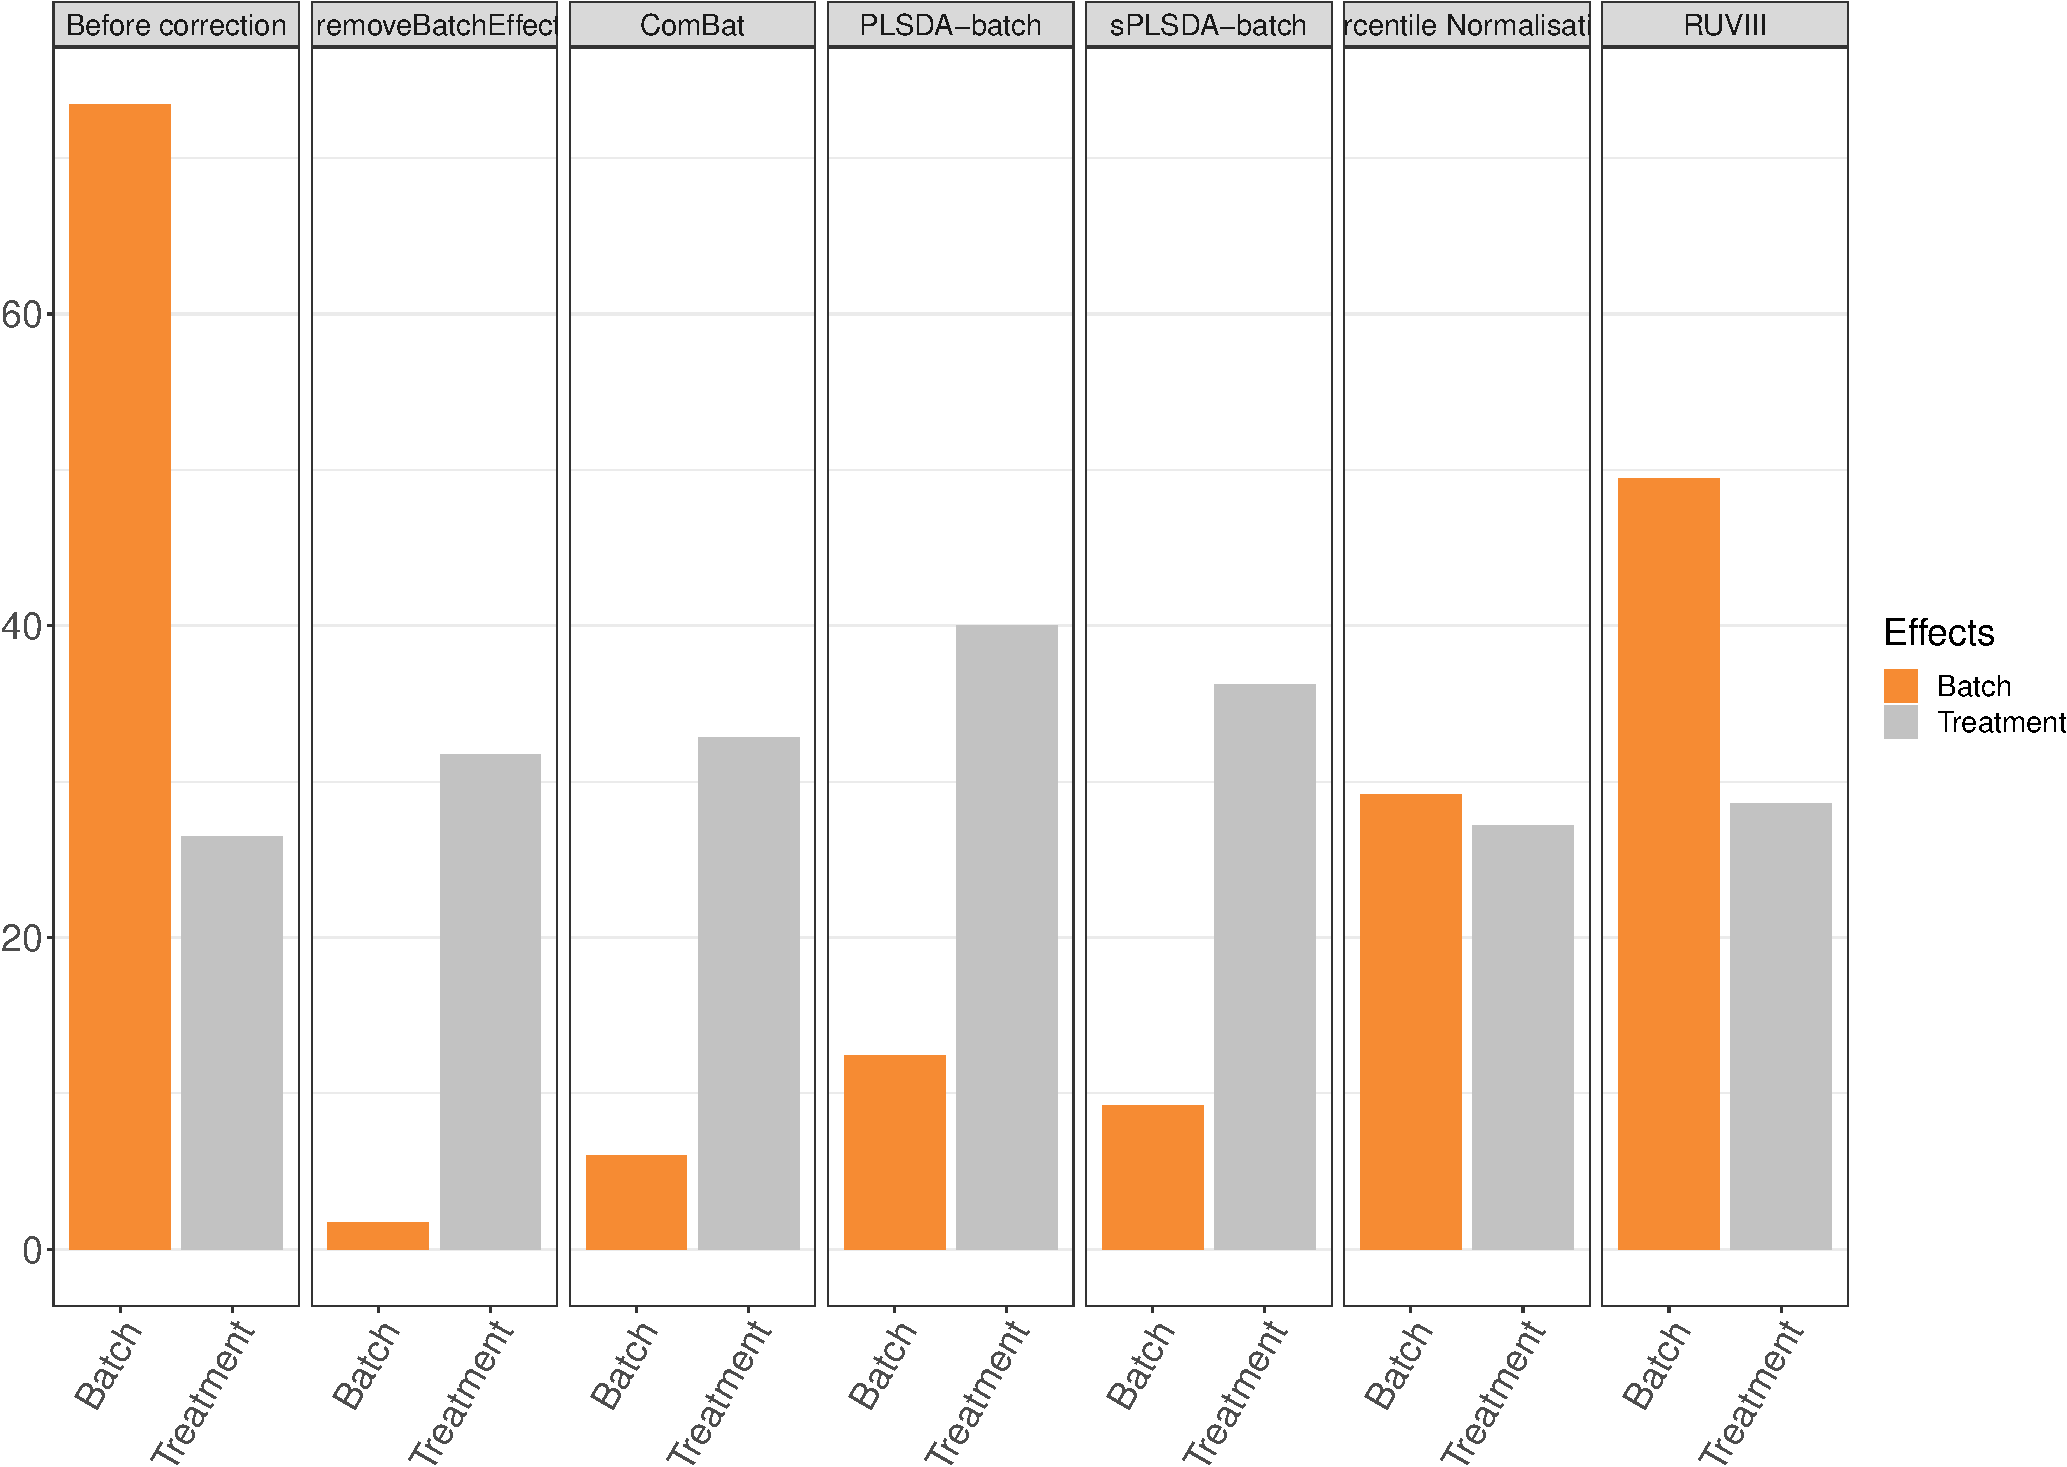
\includegraphics[width=1\linewidth]{PLSDAbatch_workflow_files/figure-latex/ADr22-1} 

}

\caption{AD study: the sum of $R^2$ values for each microbial variable before and after batch effect correction.}\label{fig:ADr22}
\end{figure}

The overall sum of \(R^2\) values indicated that removeBatchEffect removed slightly more batch variance (removeBatchEffect: 1.70, PLSDA-batch: 12.40, sPLSDA-batch: 9.25) but preserved less treatment variance (removeBatchEffect: 31.75, PLSDA-batch: 40.00, sPLSDA-batch: 36.22) than our proposed approaches

\textbf{Alignment scores}

To use the \texttt{alignment\_score()} function from \textcolor{orange}{PLSDAbatch}, we need to specify the proportion of data variance to explain (\texttt{var}), the number of nearest neighbours (\texttt{k}) and the number of principal components to estimate (\texttt{ncomp}). We then use \texttt{ggplot()} function from \textcolor{orange}{ggplot2} to visualise the results.

\begin{Shaded}
\begin{Highlighting}[]
\CommentTok{\# AD data}
\NormalTok{ad.scores }\OtherTok{\textless{}{-}} \FunctionTok{c}\NormalTok{()}
\FunctionTok{names}\NormalTok{(ad.batch) }\OtherTok{\textless{}{-}} \FunctionTok{rownames}\NormalTok{(ad.clr)}
\ControlFlowTok{for}\NormalTok{(i }\ControlFlowTok{in} \FunctionTok{seq\_len}\NormalTok{(}\FunctionTok{length}\NormalTok{(ad.corrected.list)))\{}
\NormalTok{  res }\OtherTok{\textless{}{-}} \FunctionTok{alignment\_score}\NormalTok{(}\AttributeTok{data =}\NormalTok{ ad.corrected.list[[i]], }
                         \AttributeTok{batch =}\NormalTok{ ad.batch, }
                         \AttributeTok{var =} \FloatTok{0.95}\NormalTok{, }
                         \AttributeTok{k =} \DecValTok{8}\NormalTok{, }
                         \AttributeTok{ncomp =} \DecValTok{50}\NormalTok{)}
\NormalTok{  ad.scores }\OtherTok{\textless{}{-}} \FunctionTok{c}\NormalTok{(ad.scores, res)}
\NormalTok{\}}

\NormalTok{ad.scores.df }\OtherTok{\textless{}{-}} \FunctionTok{data.frame}\NormalTok{(}\AttributeTok{scores =}\NormalTok{ ad.scores, }
                           \AttributeTok{methods =} \FunctionTok{names}\NormalTok{(ad.corrected.list))}

\NormalTok{ad.scores.df}\SpecialCharTok{$}\NormalTok{methods }\OtherTok{\textless{}{-}} \FunctionTok{factor}\NormalTok{(ad.scores.df}\SpecialCharTok{$}\NormalTok{methods, }
                               \AttributeTok{levels =} \FunctionTok{rev}\NormalTok{(}\FunctionTok{names}\NormalTok{(ad.corrected.list)))}


\FunctionTok{ggplot}\NormalTok{() }\SpecialCharTok{+} \FunctionTok{geom\_col}\NormalTok{(}\FunctionTok{aes}\NormalTok{(}\AttributeTok{x =}\NormalTok{ ad.scores.df}\SpecialCharTok{$}\NormalTok{methods, }
                        \AttributeTok{y =}\NormalTok{ ad.scores.df}\SpecialCharTok{$}\NormalTok{scores)) }\SpecialCharTok{+} 
  \FunctionTok{geom\_text}\NormalTok{(}\FunctionTok{aes}\NormalTok{(}\AttributeTok{x =}\NormalTok{ ad.scores.df}\SpecialCharTok{$}\NormalTok{methods, }
                \AttributeTok{y =}\NormalTok{ ad.scores.df}\SpecialCharTok{$}\NormalTok{scores}\SpecialCharTok{/}\DecValTok{2}\NormalTok{, }
                \AttributeTok{label =} \FunctionTok{round}\NormalTok{(ad.scores.df}\SpecialCharTok{$}\NormalTok{scores, }\DecValTok{3}\NormalTok{)), }
            \AttributeTok{size =} \DecValTok{3}\NormalTok{, }\AttributeTok{col =} \StringTok{\textquotesingle{}white\textquotesingle{}}\NormalTok{) }\SpecialCharTok{+} 
  \FunctionTok{coord\_flip}\NormalTok{() }\SpecialCharTok{+} \FunctionTok{theme\_bw}\NormalTok{() }\SpecialCharTok{+} \FunctionTok{ylab}\NormalTok{(}\StringTok{\textquotesingle{}Alignment Scores\textquotesingle{}}\NormalTok{) }\SpecialCharTok{+} 
  \FunctionTok{xlab}\NormalTok{(}\StringTok{\textquotesingle{}\textquotesingle{}}\NormalTok{) }\SpecialCharTok{+} \FunctionTok{ylim}\NormalTok{(}\DecValTok{0}\NormalTok{,}\FloatTok{0.85}\NormalTok{)}
\end{Highlighting}
\end{Shaded}

\begin{figure}

{\centering 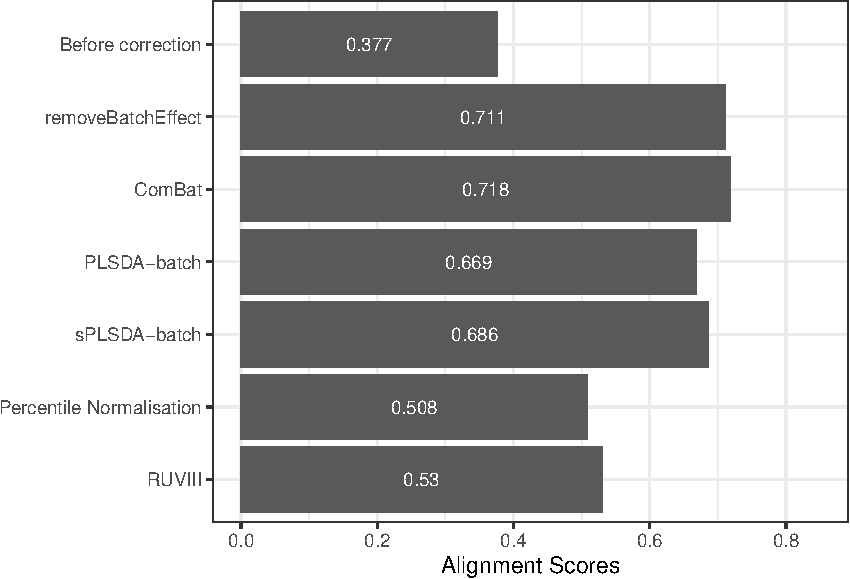
\includegraphics[width=0.6\linewidth]{PLSDAbatch_workflow_files/figure-latex/ADalignment-1} 

}

\caption{Comparison of alignment scores before and after batch effect correction using different methods for the AD data.}\label{fig:ADalignment}
\end{figure}

The alignment scores complement the PCA results, especially when batch effect removal is difficult to assess on PCA sample plots. For example in previous PCA sample plots (\textbf{Figure 7}), we observed that the samples across different batches were better mixed after batch effect correction with different methods than before, whereas the performance of difference methods was difficult to compare. Since a higher alignment score indicates that samples are better mixed, as shown in the above bar plot, Combat gave a superior performance compared to the other methods. However, with the \(R^2\) values the ComBat corrected data still included a few variables with a large proportion of batch variance (see section \textbf{other methods} method ``\(R^2\)''). Therefore, it is important to compare different techniques and outputs for an unbiased assessment. In this example, the lower alignment scores of PLSDA-batch and sPLSDA-batch corrected data might result from the difference in the PCA sample projections of the batch effect corrected matrices. The data corrected with removeBatchEffect and ComBat had a large variance in their PCA projection, while PLSDA-batch and sPLSDA-batch corrected data had a small variance. A small variance projection results in a small alignment score, as it is easy to locate the samples from the same batch as nearest neighbours. In fact, pRDA presented above (\textbf{Figure 8}) quantitatively confirmed that both PLSDA-batch and sPLSDA-batch entirely removed the batch variance \citep{wang2020multivariate}.

\hypertarget{variable-selection}{%
\section{Variable selection}\label{variable-selection}}

We use \texttt{splsda()} from \textcolor{orange}{mixOmics} to select the top 50 microbial variables that, in combination, discriminate the different treatment groups in the \textcolor{blue}{AD data}. We apply \texttt{splsda()} to the different batch effect corrected data from all methods. Then we use \texttt{upset()} from \textcolor{orange}{UpSetR} package \citep{lex2014upset} to visualise the concordance of variables selected.

In the code below, we first need to convert the list of variables selected from different method-corrected data into a data frame compatible with \texttt{upset()} using \texttt{fromList()}. We then assign different colour schemes for each variable selection.

\begin{Shaded}
\begin{Highlighting}[]
\NormalTok{ad.splsda.select }\OtherTok{\textless{}{-}} \FunctionTok{list}\NormalTok{()}
\ControlFlowTok{for}\NormalTok{(i }\ControlFlowTok{in} \FunctionTok{seq\_len}\NormalTok{(}\FunctionTok{length}\NormalTok{(ad.corrected.list)))\{}
\NormalTok{  splsda.res }\OtherTok{\textless{}{-}} \FunctionTok{splsda}\NormalTok{(}\AttributeTok{X =}\NormalTok{ ad.corrected.list[[i]], }\AttributeTok{Y =}\NormalTok{ ad.trt, }
                       \AttributeTok{ncomp =} \DecValTok{3}\NormalTok{, }\AttributeTok{keepX =} \FunctionTok{rep}\NormalTok{(}\DecValTok{50}\NormalTok{,}\DecValTok{3}\NormalTok{))}
\NormalTok{  select.res }\OtherTok{\textless{}{-}} \FunctionTok{selectVar}\NormalTok{(splsda.res, }\AttributeTok{comp =} \DecValTok{1}\NormalTok{)}\SpecialCharTok{$}\NormalTok{name}
\NormalTok{  ad.splsda.select[[i]] }\OtherTok{\textless{}{-}}\NormalTok{ select.res}
\NormalTok{\}}
\FunctionTok{names}\NormalTok{(ad.splsda.select) }\OtherTok{\textless{}{-}} \FunctionTok{names}\NormalTok{(ad.corrected.list)}

\CommentTok{\# can only visualise 5 methods}
\NormalTok{ad.splsda.select }\OtherTok{\textless{}{-}}\NormalTok{ ad.splsda.select[}\FunctionTok{seq\_len}\NormalTok{(}\DecValTok{5}\NormalTok{)]}

\NormalTok{ad.splsda.upsetR }\OtherTok{\textless{}{-}} \FunctionTok{fromList}\NormalTok{(ad.splsda.select)}

\FunctionTok{upset}\NormalTok{(ad.splsda.upsetR, }\AttributeTok{main.bar.color =} \StringTok{\textquotesingle{}gray36\textquotesingle{}}\NormalTok{,}
      \AttributeTok{sets.bar.color =} \FunctionTok{pb\_color}\NormalTok{(}\FunctionTok{c}\NormalTok{(}\DecValTok{25}\SpecialCharTok{:}\DecValTok{22}\NormalTok{,}\DecValTok{20}\NormalTok{)), }\AttributeTok{matrix.color =} \StringTok{\textquotesingle{}gray36\textquotesingle{}}\NormalTok{,}
      \AttributeTok{order.by =} \StringTok{\textquotesingle{}freq\textquotesingle{}}\NormalTok{, }\AttributeTok{empty.intersections =} \StringTok{\textquotesingle{}on\textquotesingle{}}\NormalTok{,}
      \AttributeTok{queries =} \FunctionTok{list}\NormalTok{(}\FunctionTok{list}\NormalTok{(}\AttributeTok{query =}\NormalTok{ intersects, }
                          \AttributeTok{params =} \FunctionTok{list}\NormalTok{(}\StringTok{\textquotesingle{}Before correction\textquotesingle{}}\NormalTok{), }
                          \AttributeTok{color =} \FunctionTok{pb\_color}\NormalTok{(}\DecValTok{20}\NormalTok{), }\AttributeTok{active =} \ConstantTok{TRUE}\NormalTok{),}
                     \FunctionTok{list}\NormalTok{(}\AttributeTok{query =}\NormalTok{ intersects, }
                          \AttributeTok{params =} \FunctionTok{list}\NormalTok{(}\StringTok{\textquotesingle{}removeBatchEffect\textquotesingle{}}\NormalTok{), }
                          \AttributeTok{color =} \FunctionTok{pb\_color}\NormalTok{(}\DecValTok{22}\NormalTok{), }\AttributeTok{active =} \ConstantTok{TRUE}\NormalTok{),}
                     \FunctionTok{list}\NormalTok{(}\AttributeTok{query =}\NormalTok{ intersects, }
                          \AttributeTok{params =} \FunctionTok{list}\NormalTok{(}\StringTok{\textquotesingle{}ComBat\textquotesingle{}}\NormalTok{), }
                          \AttributeTok{color =} \FunctionTok{pb\_color}\NormalTok{(}\DecValTok{23}\NormalTok{), }\AttributeTok{active =} \ConstantTok{TRUE}\NormalTok{),}
                     \FunctionTok{list}\NormalTok{(}\AttributeTok{query =}\NormalTok{ intersects, }
                          \AttributeTok{params =} \FunctionTok{list}\NormalTok{(}\StringTok{\textquotesingle{}PLSDA{-}batch\textquotesingle{}}\NormalTok{), }
                          \AttributeTok{color =} \FunctionTok{pb\_color}\NormalTok{(}\DecValTok{24}\NormalTok{), }\AttributeTok{active =} \ConstantTok{TRUE}\NormalTok{),}
                     \FunctionTok{list}\NormalTok{(}\AttributeTok{query =}\NormalTok{ intersects, }
                          \AttributeTok{params =} \FunctionTok{list}\NormalTok{(}\StringTok{\textquotesingle{}sPLSDA{-}batch\textquotesingle{}}\NormalTok{), }
                          \AttributeTok{color =} \FunctionTok{pb\_color}\NormalTok{(}\DecValTok{25}\NormalTok{), }\AttributeTok{active =} \ConstantTok{TRUE}\NormalTok{)))}
\end{Highlighting}
\end{Shaded}

\begin{figure}

{\centering 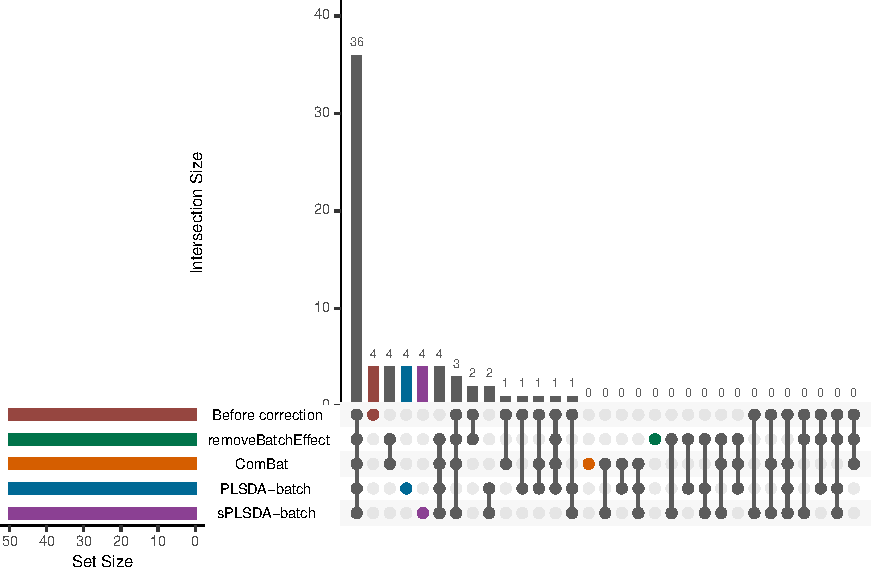
\includegraphics[width=1\linewidth]{PLSDAbatch_workflow_files/figure-latex/ADupsetR-1} 

}

\caption{UpSet plot showing overlap between variables selected from different corrected data for the AD study.}\label{fig:ADupsetR}
\end{figure}

In the above UpSet plot, the left bars indicate the number of variables selected from each data corrected with different methods. The right bar plot combined with the scatterplot show different intersection and their aggregates. We obtained a high overlap of 36 out of 50 selected variables between different corrected and uncorrected data. However, the data from each method still included unique variables that were not selected in the other corrected data, e.g., PLSDA-batch and sPLSDA-batch. As \texttt{upset()} can only include five datasets at once, we only displayed the uncorrected data and four corrected data that had been more efficiently corrected for batch effects from our previous assessments compared to the other datasets.

We then extract each intersection of selected variables between these five corrected data with \texttt{venn()} function from \textcolor{orange}{gplots}. We can also save the taxonomic information of these OTUs into a text file for further interpretation.

\begin{Shaded}
\begin{Highlighting}[]
\NormalTok{ad.splsda.select.overlap }\OtherTok{\textless{}{-}} \FunctionTok{venn}\NormalTok{(ad.splsda.select, }\AttributeTok{show.plot =} \ConstantTok{FALSE}\NormalTok{)}
\NormalTok{ad.inters.splsda }\OtherTok{\textless{}{-}} \FunctionTok{attr}\NormalTok{(ad.splsda.select.overlap, }\StringTok{\textquotesingle{}intersections\textquotesingle{}}\NormalTok{)}
\NormalTok{ad.inters.splsda.taxa }\OtherTok{\textless{}{-}} 
  \FunctionTok{lapply}\NormalTok{(ad.inters.splsda, }
         \AttributeTok{FUN =} \ControlFlowTok{function}\NormalTok{(x)\{}\FunctionTok{as.data.frame}\NormalTok{(AD\_data}\SpecialCharTok{$}\NormalTok{FullData}\SpecialCharTok{$}\NormalTok{taxa[x, ])\})}
\FunctionTok{capture.output}\NormalTok{(ad.inters.splsda.taxa, }
               \AttributeTok{file =} \StringTok{"GeneratedData/ADselected\_50\_splsda.txt"}\NormalTok{)}
\end{Highlighting}
\end{Shaded}

\hypertarget{summary}{%
\section{Summary}\label{summary}}

This vignette presents a complete framework for batch effect management in microbiome data. The first step includes pre-processing, with pre-filtering to remove low-count samples and variables, and data transformation to handle compositional data characteristics. For this step, we advise against using relative abundance data that are compositional, if possible. Visual tools, such as PCA, boxplots, density plots and heatmap, and quantitative approach pRDA are then applied to detect batch effects. When the batch effect is very weak, for example as informed by a very small proportion of variance explained by batch with pRDA, or difficult to visualise with PCA, then there may be no need to manage batch effects. However, when the batch effect is strong, two solutions are to either account for batch effects, or to correct for batch effects from the original data. For either solution, the batch x treatment design matters. If nested, we can only account for batch effects with a linear mixed model. If unbalanced but not nested, we can account for batch effects with any linear models or remove them using weighted PLSDA-batch. Regarding different batch effects, our proposed method PLSDA-batch is more appropriate for a weak batch effect, while sPLSDA-batch for a strong batch effect.

We usually assume batch grouping information is known. When the batch information is unknown, methods such as SVA estimate batch effects from the variables least affected by treatment effects, while RUV4 and RUVIII estimate batch effects from negative control variables or/and sample replicates. For the latter, negative control variables and sample replicates should capture the complete batch variation, if not, there may be a risk that batch effects cannot be completely considered or removed. We emphasised on this point in the \textcolor{blue}{AD} and the \textcolor{olive}{HFHS} studies. For these methods that can estimate batch effects, the estimated batch effects are independent of treatment effects. If a correlation between batch and treatment exists, this correlation cannot be estimated. Spurious correlation between batch and treatment effects may also be present, for example SVA, which estimates batch effects from the variables that may still include more or less treatment effects.

In addition, most methods assume systematic batch effects across the whole dataset. This is the case of ComBat, where we recommend assessing the model's validity first.

The next critical step is to assess the efficacy of batch effect management for a given method. Such assessment is often implicit in methods that account for batch effects. In contrast, the methods that remove batch effects can be assessed by comparing the data before and after correction. All methods we have presented for batch effect detection can be used for assessing batch effect correction. We can also calculate the explained variance \(R^2\) of each microbial variable for batch and treatment covariate respectively, as well as alignment scores measuring the performance of mixing samples across batches. We also have noted that some methods may not be very sensitive. For example, PCA plots rely on somewhat subjective evaluation of batch and treatment variation visualisation, and alignment scores only measure the performance of mixing samples. Therefore, a reliable conclusion should be made based on multiple assessment methods.

Once batch effects are removed, downstream analysis such as multivariate discriminant analysis, or univariate differential analysis can be performed. Multivariate methods may be more suitable for microbiome data analysis since microbial variables are naturally correlated because of mutual interactions.

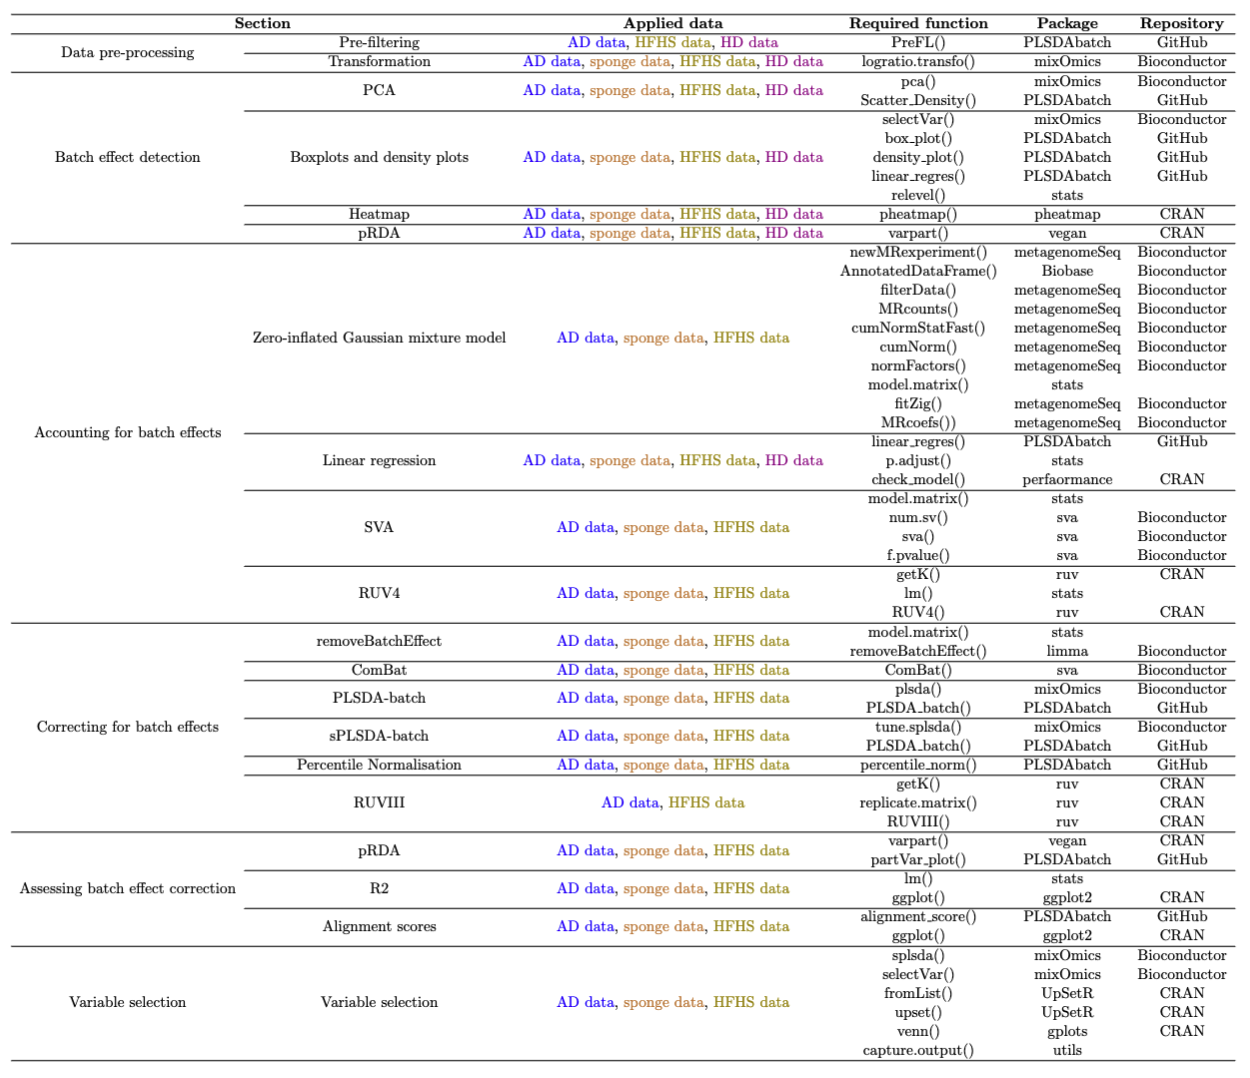
\includegraphics{./figures/function_description.png}
\textbf{Table 2: A summary of all functions in each section.}

\hypertarget{references}{%
\section{References}\label{references}}

\hypertarget{supplementary-materials-for-batch-effects-management-in-case-studies}{%
\chapter{Supplementary Materials for Batch Effects Management in Case Studies}\label{supplementary-materials-for-batch-effects-management-in-case-studies}}

\hypertarget{sponge-data}{%
\section{Sponge data}\label{sponge-data}}

\hypertarget{data-pre-processing-1}{%
\subsection{Data pre-processing}\label{data-pre-processing-1}}

\hypertarget{pre-filtering-1}{%
\subsubsection{Pre-filtering}\label{pre-filtering-1}}

We load the \textcolor{brown}{sponge data} stored internally with function \texttt{data()}.

\begin{Shaded}
\begin{Highlighting}[]
\CommentTok{\# Sponge data}
\FunctionTok{data}\NormalTok{(}\StringTok{\textquotesingle{}sponge\_data\textquotesingle{}}\NormalTok{) }
\NormalTok{sponge.tss }\OtherTok{\textless{}{-}}\NormalTok{ sponge\_data}\SpecialCharTok{$}\NormalTok{X.tss}
\FunctionTok{dim}\NormalTok{(sponge.tss)}
\end{Highlighting}
\end{Shaded}

\begin{verbatim}
## [1] 32 24
\end{verbatim}

\begin{Shaded}
\begin{Highlighting}[]
\CommentTok{\# zero proportion}
\FunctionTok{mean}\NormalTok{(sponge.tss }\SpecialCharTok{==} \DecValTok{0}\NormalTok{)}
\end{Highlighting}
\end{Shaded}

\begin{verbatim}
## [1] 0.5455729
\end{verbatim}

The \textcolor{brown}{sponge data} include the relative abundance of 24 OTUs and 32 samples. Given the small number of OTUs we advise not to pre-filter the data.

\hypertarget{transformation-1}{%
\subsubsection{Transformation}\label{transformation-1}}

Prior to CLR transformation, we recommend adding 0.01 as the offset for the \textcolor{brown}{sponge data} - that are relative abundance data. We use \texttt{logratio.transfo()} function in \textcolor{orange}{mixOmics} package to CLR transform the data.

\begin{Shaded}
\begin{Highlighting}[]
\NormalTok{sponge.clr }\OtherTok{\textless{}{-}} \FunctionTok{logratio.transfo}\NormalTok{(}\AttributeTok{X =}\NormalTok{ sponge.tss, }\AttributeTok{logratio =} \StringTok{\textquotesingle{}CLR\textquotesingle{}}\NormalTok{, }\AttributeTok{offset =} \FloatTok{0.01}\NormalTok{)}

\FunctionTok{class}\NormalTok{(sponge.clr) }\OtherTok{\textless{}{-}} \StringTok{\textquotesingle{}matrix\textquotesingle{}}
\end{Highlighting}
\end{Shaded}

\hypertarget{batch-effect-detection-1}{%
\subsection{Batch effect detection}\label{batch-effect-detection-1}}

\hypertarget{pca-1}{%
\subsubsection{PCA}\label{pca-1}}

We apply \texttt{pca()} function from \textcolor{orange}{mixOmics} package to the \textcolor{brown}{sponge data} and \texttt{Scatter\_Density()} function from \textcolor{orange}{PLSDAbatch} to represent the PCA sample plot with densities.

\begin{Shaded}
\begin{Highlighting}[]
\NormalTok{sponge.pca.before }\OtherTok{\textless{}{-}} \FunctionTok{pca}\NormalTok{(sponge.clr, }\AttributeTok{ncomp =} \DecValTok{3}\NormalTok{, }\AttributeTok{scale =} \ConstantTok{TRUE}\NormalTok{)}

\NormalTok{sponge.batch }\OtherTok{\textless{}{-}}\NormalTok{ sponge\_data}\SpecialCharTok{$}\NormalTok{Y.bat}
\NormalTok{sponge.trt }\OtherTok{\textless{}{-}}\NormalTok{ sponge\_data}\SpecialCharTok{$}\NormalTok{Y.trt}

\FunctionTok{Scatter\_Density}\NormalTok{(}\AttributeTok{object =}\NormalTok{ sponge.pca.before, }
                \AttributeTok{batch =}\NormalTok{ sponge.batch, }
                \AttributeTok{trt =}\NormalTok{ sponge.trt, }\AttributeTok{title =} \StringTok{\textquotesingle{}Sponge data\textquotesingle{}}\NormalTok{, }
                \AttributeTok{trt.legend.title =} \StringTok{\textquotesingle{}Tissue types\textquotesingle{}}\NormalTok{)}
\end{Highlighting}
\end{Shaded}

\begin{figure}

{\centering 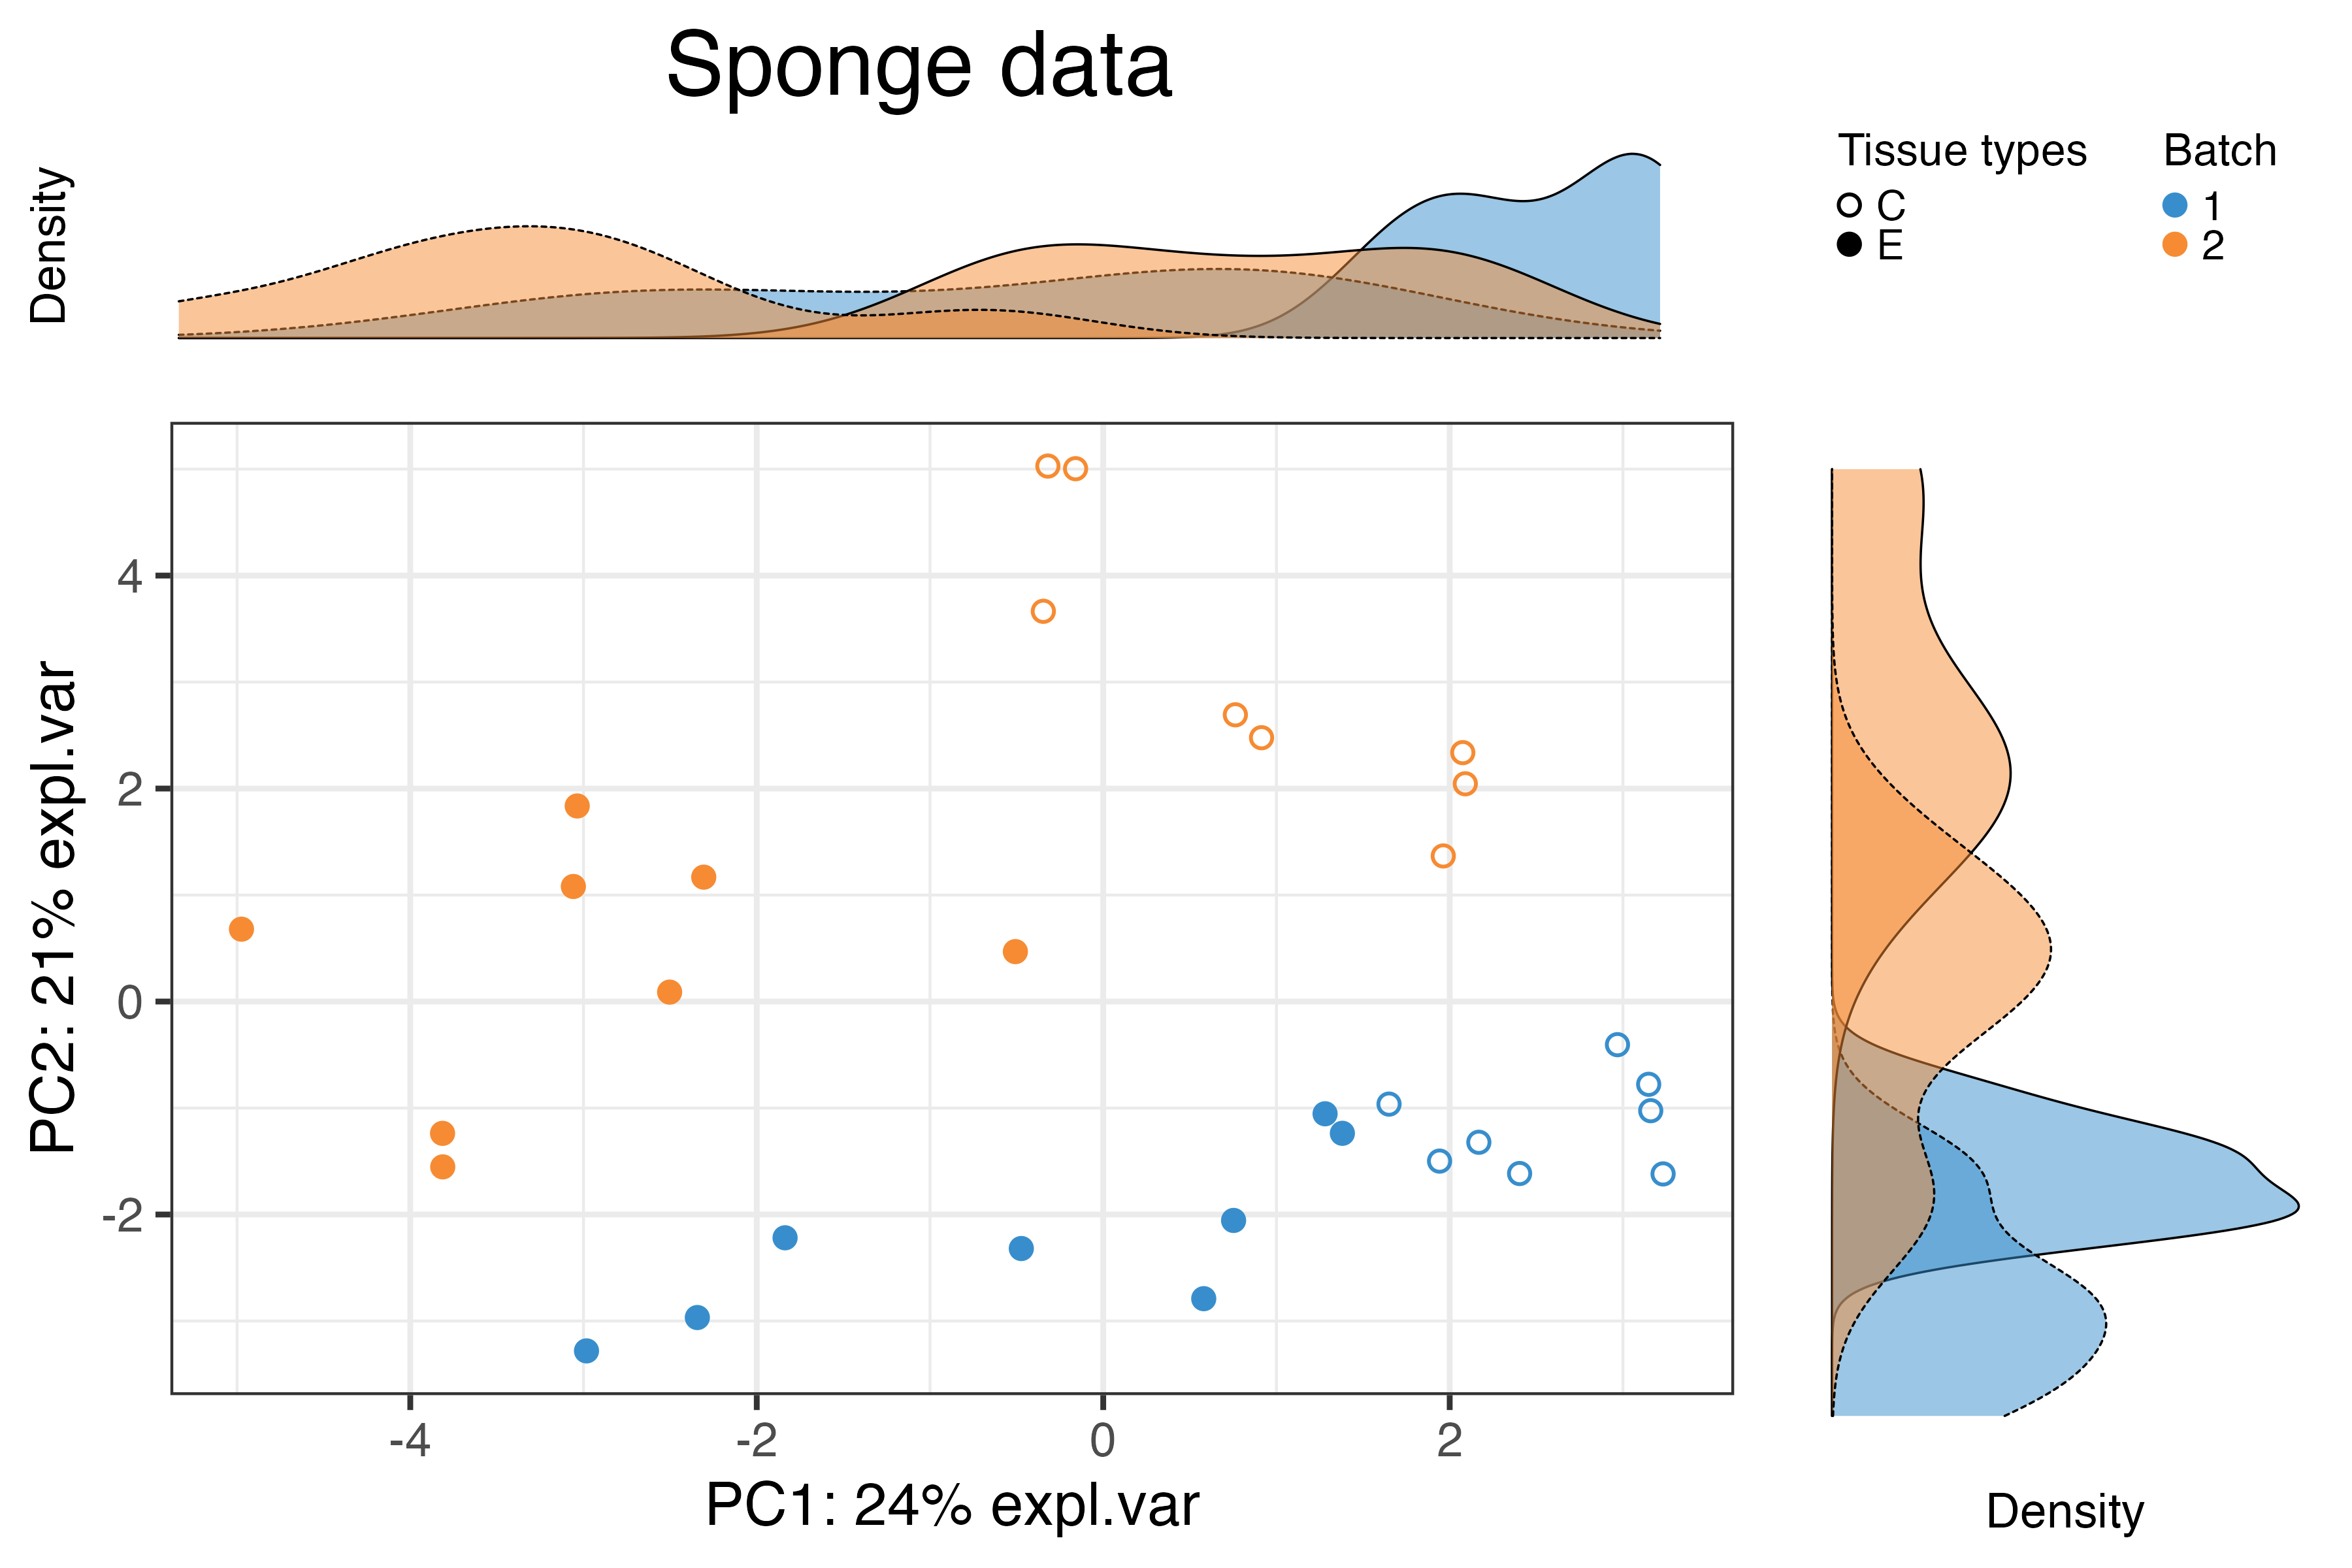
\includegraphics[width=0.6\linewidth]{PLSDAbatch_workflow_files/figure-latex/SpongepcaBefore-1} 

}

\caption{The PCA sample plot with densities in the sponge data.}\label{fig:SpongepcaBefore}
\end{figure}

In the above figure, the tissue variation (effects of interest) accounted for 24\% of data variance on component 1, while the gel variation (batch effects) for 21\% on component 2. Therefore, the batch effect is slightly weaker than the treatment effect in the \textcolor{brown}{sponge data}.

\hypertarget{heatmap-1}{%
\subsubsection{Heatmap}\label{heatmap-1}}

We produce a heatmap using \textcolor{orange}{pheatmap} package. The data first need to be scaled on both OTUs and samples.

\begin{Shaded}
\begin{Highlighting}[]
\CommentTok{\# scale the clr data on both OTUs and samples}
\NormalTok{sponge.clr.s }\OtherTok{\textless{}{-}} \FunctionTok{scale}\NormalTok{(sponge.clr, }\AttributeTok{center =}\NormalTok{ T, }\AttributeTok{scale =}\NormalTok{ T)}
\NormalTok{sponge.clr.ss }\OtherTok{\textless{}{-}} \FunctionTok{scale}\NormalTok{(}\FunctionTok{t}\NormalTok{(sponge.clr.s), }\AttributeTok{center =}\NormalTok{ T, }\AttributeTok{scale =}\NormalTok{ T)}

\NormalTok{sponge.anno\_col }\OtherTok{\textless{}{-}} \FunctionTok{data.frame}\NormalTok{(}\AttributeTok{Batch =}\NormalTok{ sponge.batch, }\AttributeTok{Tissue =}\NormalTok{ sponge.trt)}
\NormalTok{sponge.anno\_colors }\OtherTok{\textless{}{-}} \FunctionTok{list}\NormalTok{(}\AttributeTok{Batch =} \FunctionTok{color.mixo}\NormalTok{(}\DecValTok{1}\SpecialCharTok{:}\DecValTok{2}\NormalTok{), }
                           \AttributeTok{Tissue =} \FunctionTok{pb\_color}\NormalTok{(}\DecValTok{1}\SpecialCharTok{:}\DecValTok{2}\NormalTok{))}
\FunctionTok{names}\NormalTok{(sponge.anno\_colors}\SpecialCharTok{$}\NormalTok{Batch) }\OtherTok{=} \FunctionTok{levels}\NormalTok{(sponge.batch)}
\FunctionTok{names}\NormalTok{(sponge.anno\_colors}\SpecialCharTok{$}\NormalTok{Tissue) }\OtherTok{=} \FunctionTok{levels}\NormalTok{(sponge.trt)}

\FunctionTok{pheatmap}\NormalTok{(sponge.clr.ss, }
         \AttributeTok{cluster\_rows =}\NormalTok{ F, }
         \AttributeTok{fontsize\_row =} \DecValTok{4}\NormalTok{, }
         \AttributeTok{fontsize\_col =} \DecValTok{6}\NormalTok{,}
         \AttributeTok{fontsize =} \DecValTok{8}\NormalTok{,}
         \AttributeTok{clustering\_distance\_rows =} \StringTok{\textquotesingle{}euclidean\textquotesingle{}}\NormalTok{,}
         \AttributeTok{clustering\_method =} \StringTok{\textquotesingle{}ward.D\textquotesingle{}}\NormalTok{,}
         \AttributeTok{treeheight\_row =} \DecValTok{30}\NormalTok{,}
         \AttributeTok{annotation\_col =}\NormalTok{ sponge.anno\_col,}
         \AttributeTok{annotation\_colors =}\NormalTok{ sponge.anno\_colors,}
         \AttributeTok{border\_color =} \StringTok{\textquotesingle{}NA\textquotesingle{}}\NormalTok{,}
         \AttributeTok{main =} \StringTok{\textquotesingle{}Sponge data {-} Scaled\textquotesingle{}}\NormalTok{)}
\end{Highlighting}
\end{Shaded}

\begin{figure}

{\centering 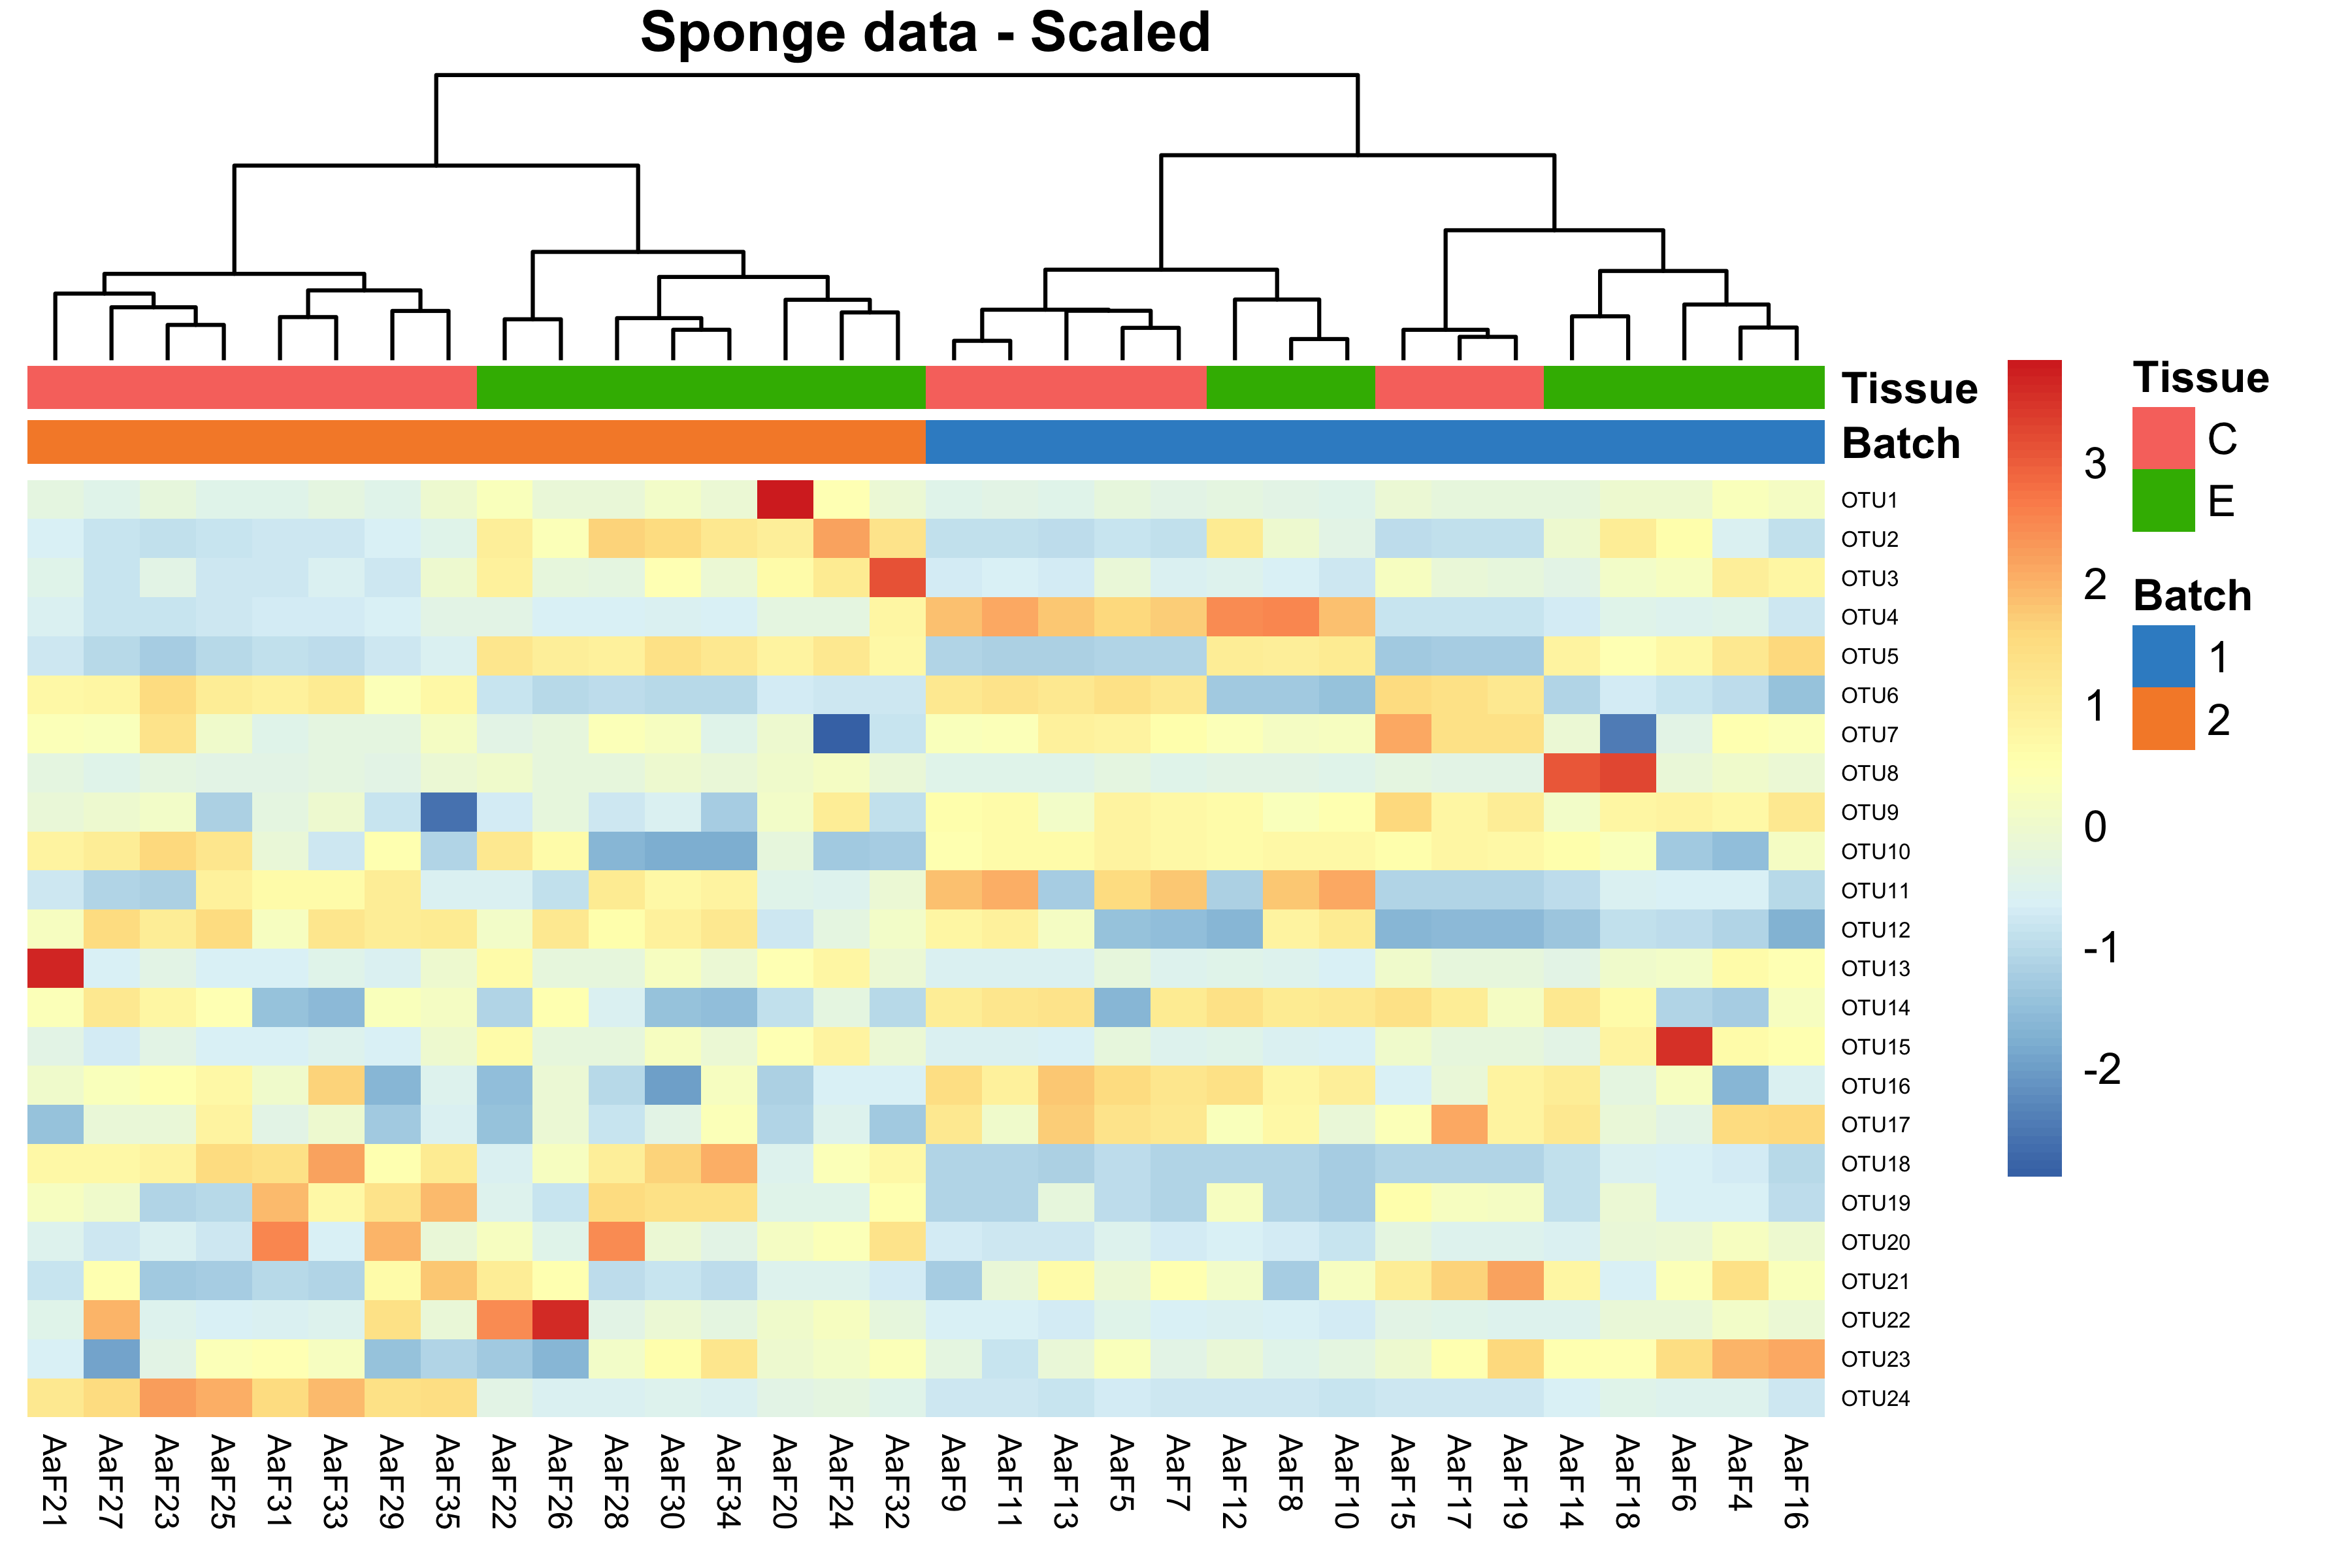
\includegraphics[width=0.9\linewidth]{PLSDAbatch_workflow_files/figure-latex/Spongeheatmap-1} 

}

\caption{Hierarchical clustering for samples in the sponge data.}\label{fig:Spongeheatmap}
\end{figure}

In the heatmap, samples in the \textcolor{brown}{sponge data} were clustered or grouped by batches instead of tissues, indicating a batch effect.

\hypertarget{prda-1}{%
\subsubsection{pRDA}\label{prda-1}}

We apply pRDA with \texttt{varpart()} function from \textcolor{orange}{vegan} R package.

\begin{Shaded}
\begin{Highlighting}[]
\NormalTok{sponge.factors.df }\OtherTok{\textless{}{-}} \FunctionTok{data.frame}\NormalTok{(}\AttributeTok{trt =}\NormalTok{ sponge.trt, }
                                \AttributeTok{batch =}\NormalTok{ sponge.batch)}
\NormalTok{sponge.rda.before }\OtherTok{\textless{}{-}} \FunctionTok{varpart}\NormalTok{(sponge.clr, }\SpecialCharTok{\textasciitilde{}}\NormalTok{ trt, }\SpecialCharTok{\textasciitilde{}}\NormalTok{ batch, }
                             \AttributeTok{data =}\NormalTok{ sponge.factors.df, }
                             \AttributeTok{scale =}\NormalTok{ T)}
\NormalTok{sponge.rda.before}\SpecialCharTok{$}\NormalTok{part}\SpecialCharTok{$}\NormalTok{indfract}
\end{Highlighting}
\end{Shaded}

\begin{verbatim}
##                 Df R.squared Adj.R.squared Testable
## [a] = X1|X2      1        NA    0.16572246     TRUE
## [b] = X2|X1      1        NA    0.16396277     TRUE
## [c]              0        NA   -0.01063501    FALSE
## [d] = Residuals NA        NA    0.68094977    FALSE
\end{verbatim}

In the result, \texttt{X1} and \texttt{X2} represent the first and second covariates fitted in the model. \texttt{{[}a{]}}, \texttt{{[}b{]}} represent the independent proportion of variance explained by \texttt{X1} and \texttt{X2} respectively, and \texttt{{[}c{]}} represents the intersection variance shared between \texttt{X1} and \texttt{X2}. The \textcolor{brown}{sponge data} have a completely balanced batch x treatment design, so there was no intersection variance (indicated in line \texttt{{[}c{]}}, Adj.R.squared = -0.01) detected. The proportion of treatment and batch variance was nearly equal as indicated in lines \texttt{{[}a{]}} and \texttt{{[}b{]}}.

\hypertarget{managing-batch-effects-1}{%
\subsection{Managing batch effects}\label{managing-batch-effects-1}}

\hypertarget{accounting-for-batch-effects}{%
\subsubsection{Accounting for batch effects}\label{accounting-for-batch-effects}}

The methods that we use to account for batch effects include the method designed for microbiome data: zero-inflated Gaussian (ZIG) mixture model and the methods adapted for microbiome data: linear regression, SVA and RUV4. Among them, SVA and RUV4 are designed for unknown batch effects.

As the ZIG model is applicable to counts data, the \textcolor{brown}{sponge data} are not qualified for this model. We therefore only apply the methods that can be adapted for microbiome data.

\textbf{Linear regression}

Linear regression is conducted with \texttt{linear\_regres()} function in \textcolor{orange}{PLSDAbatch}. We integrated the \textcolor{orange}{performance} package that assesses performance of regression models into our function \texttt{linear\_regres()}. Therefore, we can apply \texttt{check\_model()} from \textcolor{orange}{performance} to the outputs from \texttt{linear\_regres()} to diagnose the validity of the model fitted with treatment and batch effects for each variable \citep{daniel2020performance}. We can extract performance measurements such as adjusted R2, RMSE, RSE, AIC and BIC for the models fitted with and without batch effects, which are also the outputs of \texttt{linear\_regres()}.

We apply \texttt{type\ =\ "linear\ model"} to the \textcolor{brown}{sponge data} because of the balanced batch x treatment design.

\begin{Shaded}
\begin{Highlighting}[]
\NormalTok{sponge.clr }\OtherTok{\textless{}{-}}\NormalTok{ sponge.clr[}\DecValTok{1}\SpecialCharTok{:}\FunctionTok{nrow}\NormalTok{(sponge.clr), }\DecValTok{1}\SpecialCharTok{:}\FunctionTok{ncol}\NormalTok{(sponge.clr)]}
\NormalTok{sponge.lm }\OtherTok{\textless{}{-}} \FunctionTok{linear\_regres}\NormalTok{(}\AttributeTok{data =}\NormalTok{ sponge.clr, }
                           \AttributeTok{trt =}\NormalTok{ sponge.trt, }
                           \AttributeTok{batch.fix =}\NormalTok{ sponge.batch, }
                           \AttributeTok{type =} \StringTok{\textquotesingle{}linear model\textquotesingle{}}\NormalTok{)}

\NormalTok{sponge.p }\OtherTok{\textless{}{-}} \FunctionTok{sapply}\NormalTok{(sponge.lm}\SpecialCharTok{$}\NormalTok{lm.table, }\ControlFlowTok{function}\NormalTok{(x)\{x}\SpecialCharTok{$}\NormalTok{coefficients[}\DecValTok{2}\NormalTok{,}\DecValTok{4}\NormalTok{]\})}
\NormalTok{sponge.p.adj }\OtherTok{\textless{}{-}} \FunctionTok{p.adjust}\NormalTok{(}\AttributeTok{p =}\NormalTok{ sponge.p, }\AttributeTok{method =} \StringTok{\textquotesingle{}fdr\textquotesingle{}}\NormalTok{)}

\FunctionTok{check\_model}\NormalTok{(sponge.lm}\SpecialCharTok{$}\NormalTok{model}\SpecialCharTok{$}\NormalTok{OTU2)}
\end{Highlighting}
\end{Shaded}

\begin{figure}

{\centering \includegraphics[width=1\linewidth]{PLSDAbatch_workflow_files/figure-latex/Spongelm-1} 

}

\caption{Diagnostic plots for the model fitted with batch effects of "OTU2" in the sponge data.}\label{fig:Spongelm}
\end{figure}

To diagnose the validity of the model fitted with both treatment and batch effects, we use different plots to check the assumptions of each microbial variable. For example, the diagnostic plots of ``OTU2'' are shown in the above figure panel. The simulated data under the fitted model were not very close to the real data (shown as green line), indicating an imperfect fitness (top panel). The linearity (or homoscedasticity) and homogeneity of variance were not satisfied. The correlation between batch (\texttt{batch.fix}) and treatment (\texttt{trt}) effects was very low, indicating a good model with low collinearity. Some samples could be classified as outliers with a Cook's distance larger than or equal to 0.5, for example, ``21'', ``15'', ``7'', ``1'' and ``13'' (middle panel). The distribution of residuals was not close to normal (bottom panel). For the microbial variables with some assumptions not met, we should be careful about their results.

For performance measurements of models fitted with or without batch effects, we show an example of the results for some variables.

\begin{Shaded}
\begin{Highlighting}[]
\FunctionTok{head}\NormalTok{(sponge.lm}\SpecialCharTok{$}\NormalTok{adj.R2)}
\end{Highlighting}
\end{Shaded}

\begin{verbatim}
##         trt.only  trt.batch
## OTU1  0.06423228 0.05701977
## OTU2  0.60492094 0.67117014
## OTU3  0.19003076 0.18125188
## OTU4 -0.03327738 0.23731780
## OTU5  0.97483298 0.97643741
## OTU6  0.97496003 0.97634939
\end{verbatim}

If the adjusted \(R^2\) of the model with both treatment and batch effects is larger than the model with treatment effects only, e.g., OTU2, OTU4, OTU5 and OTU6, the model fitted with batch effects explains more data variance, and is thus better than the model without batch effects. Otherwise, the batch effect is not necessary to be added into the linear model.

We next look at the AIC of models fitted with or without batch effects.

\begin{Shaded}
\begin{Highlighting}[]
\FunctionTok{head}\NormalTok{(sponge.lm}\SpecialCharTok{$}\NormalTok{AIC)}
\end{Highlighting}
\end{Shaded}

\begin{verbatim}
##       trt.only  trt.batch
## OTU1 47.901506 49.0623531
## OTU2 74.001621 69.0433180
## OTU3 -5.630456 -4.3703385
## OTU4 90.699895 81.8982606
## OTU5 21.727333 20.5345128
## OTU6  1.196912  0.2853681
\end{verbatim}

A lower AIC indicates a better fit. Both results of the adjusted \(R^2\) and AIC were consistent on model selection for the listed OTUs.

\textbf{SVA}

SVA accounts for unknown batch effects. Here we assume that the batch grouping information in the \textcolor{brown}{sponge data} is unknown. We first build two design matrices with (\texttt{sponge.mod}) and without (\texttt{sponge.mod0}) treatment grouping information generated with \texttt{model.matrix()} function from \textcolor{orange}{stats}. We then use \texttt{num.sv()} from \textcolor{orange}{sva} package to determine the number of batch variables \texttt{n.sv} that is used to estimate batch effects in function \texttt{sva()}.

\begin{Shaded}
\begin{Highlighting}[]
\CommentTok{\# estimate batch matrix}
\NormalTok{sponge.mod }\OtherTok{\textless{}{-}} \FunctionTok{model.matrix}\NormalTok{( }\SpecialCharTok{\textasciitilde{}}\NormalTok{ sponge.trt)}
\NormalTok{sponge.mod0 }\OtherTok{\textless{}{-}} \FunctionTok{model.matrix}\NormalTok{( }\SpecialCharTok{\textasciitilde{}} \DecValTok{1}\NormalTok{, }\AttributeTok{data =}\NormalTok{ sponge.trt)}
\NormalTok{sponge.sva.n }\OtherTok{\textless{}{-}} \FunctionTok{num.sv}\NormalTok{(}\AttributeTok{dat =} \FunctionTok{t}\NormalTok{(sponge.clr), }\AttributeTok{mod =}\NormalTok{ sponge.mod, }\AttributeTok{method =} \StringTok{\textquotesingle{}leek\textquotesingle{}}\NormalTok{)}
\NormalTok{sponge.sva }\OtherTok{\textless{}{-}} \FunctionTok{sva}\NormalTok{(}\FunctionTok{t}\NormalTok{(sponge.clr), sponge.mod, sponge.mod0, }\AttributeTok{n.sv =}\NormalTok{ sponge.sva.n)}
\end{Highlighting}
\end{Shaded}

\begin{verbatim}
## Number of significant surrogate variables is:  1 
## Iteration (out of 5 ):1  2  3  4  5
\end{verbatim}

The estimated batch effects are then applied to \texttt{f.pvalue()} to calculate the P-values of treatment effects. The estimated batch effects in SVA are assumed to be independent of the treatment effects. However, SVA considers some correlation between batch and treatment effects \citep{wang2020managing}.

\begin{Shaded}
\begin{Highlighting}[]
\CommentTok{\# include estimated batch effects in the linear model}
\NormalTok{sponge.mod.batch }\OtherTok{\textless{}{-}} \FunctionTok{cbind}\NormalTok{(sponge.mod, sponge.sva}\SpecialCharTok{$}\NormalTok{sv)}
\NormalTok{sponge.mod0.batch }\OtherTok{\textless{}{-}} \FunctionTok{cbind}\NormalTok{(sponge.mod0, sponge.sva}\SpecialCharTok{$}\NormalTok{sv)}
\NormalTok{sponge.sva.p }\OtherTok{\textless{}{-}} \FunctionTok{f.pvalue}\NormalTok{(}\FunctionTok{t}\NormalTok{(sponge.clr), sponge.mod.batch, sponge.mod0.batch)}
\NormalTok{sponge.sva.p.adj }\OtherTok{\textless{}{-}} \FunctionTok{p.adjust}\NormalTok{(sponge.sva.p, }\AttributeTok{method =} \StringTok{\textquotesingle{}fdr\textquotesingle{}}\NormalTok{)}
\end{Highlighting}
\end{Shaded}

\textbf{RUV4}

Before applying RUV4 (\texttt{RUV4()} from \textcolor{orange}{ruv} package), we need to specify negative control variables and the number of batch variables to estimate. We can use the empirical negative controls that are not significantly differentially abundant (adjusted P \textgreater{} 0.05) from a linear regression with the treatment information as the only covariate.

We use a loop to fit a linear regression for each microbial variable and adjust P values of treatment effects for multiple comparisons with \texttt{p.adjust()} from \textcolor{orange}{stats}. The empirical negative controls are then extracted according to the adjusted P values.

\begin{Shaded}
\begin{Highlighting}[]
\CommentTok{\# empirical negative controls}
\NormalTok{sponge.empir.p }\OtherTok{\textless{}{-}} \FunctionTok{c}\NormalTok{()}
\ControlFlowTok{for}\NormalTok{(e }\ControlFlowTok{in} \DecValTok{1}\SpecialCharTok{:}\FunctionTok{ncol}\NormalTok{(sponge.clr))\{}
\NormalTok{  sponge.empir.lm }\OtherTok{\textless{}{-}} \FunctionTok{lm}\NormalTok{(sponge.clr[,e] }\SpecialCharTok{\textasciitilde{}}\NormalTok{ sponge.trt)}
\NormalTok{  sponge.empir.p[e] }\OtherTok{\textless{}{-}} \FunctionTok{summary}\NormalTok{(sponge.empir.lm)}\SpecialCharTok{$}\NormalTok{coefficients[}\DecValTok{2}\NormalTok{,}\DecValTok{4}\NormalTok{]}
\NormalTok{\}}
\NormalTok{sponge.empir.p.adj }\OtherTok{\textless{}{-}} \FunctionTok{p.adjust}\NormalTok{(}\AttributeTok{p =}\NormalTok{ sponge.empir.p, }\AttributeTok{method =} \StringTok{\textquotesingle{}fdr\textquotesingle{}}\NormalTok{)}
\NormalTok{sponge.nc }\OtherTok{\textless{}{-}}\NormalTok{ sponge.empir.p.adj }\SpecialCharTok{\textgreater{}} \FloatTok{0.05}
\end{Highlighting}
\end{Shaded}

The number of batch variables \texttt{k} can be determined using \texttt{getK()} function.

\begin{Shaded}
\begin{Highlighting}[]
\CommentTok{\# estimate k}
\NormalTok{sponge.k.res }\OtherTok{\textless{}{-}} \FunctionTok{getK}\NormalTok{(}\AttributeTok{Y =}\NormalTok{ sponge.clr, }\AttributeTok{X =}\NormalTok{ sponge.trt, }\AttributeTok{ctl =}\NormalTok{ sponge.nc)}
\NormalTok{sponge.k }\OtherTok{\textless{}{-}}\NormalTok{ sponge.k.res}\SpecialCharTok{$}\NormalTok{k}
\NormalTok{sponge.k }\OtherTok{\textless{}{-}} \FunctionTok{ifelse}\NormalTok{(sponge.k }\SpecialCharTok{!=} \DecValTok{0}\NormalTok{, sponge.k, }\DecValTok{1}\NormalTok{)}
\end{Highlighting}
\end{Shaded}

We then apply \texttt{RUV4()} with known treatment variables, estimated negative control variables and \texttt{k} batch variables. The calculated P values also need to be adjusted for multiple comparisons.

\begin{Shaded}
\begin{Highlighting}[]
\NormalTok{sponge.ruv4 }\OtherTok{\textless{}{-}} \FunctionTok{RUV4}\NormalTok{(}\AttributeTok{Y =}\NormalTok{ sponge.clr, }\AttributeTok{X =}\NormalTok{ sponge.trt, }
                    \AttributeTok{ctl =}\NormalTok{ sponge.nc, }\AttributeTok{k =}\NormalTok{ sponge.k) }
\NormalTok{sponge.ruv4.p }\OtherTok{\textless{}{-}}\NormalTok{ sponge.ruv4}\SpecialCharTok{$}\NormalTok{p}
\NormalTok{sponge.ruv4.p.adj }\OtherTok{\textless{}{-}} \FunctionTok{p.adjust}\NormalTok{(sponge.ruv4.p, }\AttributeTok{method =} \StringTok{"fdr"}\NormalTok{)}
\end{Highlighting}
\end{Shaded}

Note: A package named \textcolor{orange}{RUVSeq} has been developed for count data. It provides \texttt{RUVg()} using negative control variables, and also other functions \texttt{RUVs()} and \texttt{RUVr()} using sample replicates \citep{moskovicz2020skin} or residuals from the regression on treatment effects to estimate and then account for latent batch effects. However, for CLR-transformed data, we still recommend the standard \textcolor{orange}{ruv} package.

\hypertarget{correcting-for-batch-effects}{%
\subsubsection{Correcting for batch effects}\label{correcting-for-batch-effects}}

The methods that we use to correct for batch effects include removeBatchEffect, ComBat, PLSDA-batch, sPLSDA-batch, Percentile Normalisation and RUVIII. Among them, RUVIII is designed for unknown batch effects. Except RUVIII that requires sample replicates which the \textcolor{brown}{sponge data} do not have, these methods were all applied to and illustrated with the \textcolor{brown}{sponge data}.

\textbf{removeBatchEffect}

The \texttt{removeBatchEffect()} function is implemented in \textcolor{orange}{limma} package. The design matrix (\texttt{design}) with treatment grouping information can be generated with \texttt{model.matrix()} function from \textcolor{orange}{stats} as shown in section \textbf{accounting for batch effects} method ``SVA''.

Here we use \texttt{removeBatchEffect()} function with batch grouping information (\texttt{batch}) and treatment design matrix (\texttt{design}) to calculate batch effect corrected data \texttt{sponge.rBE}.

\begin{Shaded}
\begin{Highlighting}[]
\NormalTok{sponge.rBE }\OtherTok{\textless{}{-}} \FunctionTok{t}\NormalTok{(}\FunctionTok{removeBatchEffect}\NormalTok{(}\FunctionTok{t}\NormalTok{(sponge.clr), }\AttributeTok{batch =}\NormalTok{ sponge.batch, }
                                  \AttributeTok{design =}\NormalTok{ sponge.mod))}
\end{Highlighting}
\end{Shaded}

\textbf{ComBat}

The \texttt{ComBat()} function (from \textcolor{orange}{sva} package) is implemented as parametric or non-parametric correction with option \texttt{par.prior}. Under a parametric adjustment, we can assess the model's validity with \texttt{prior.plots\ =\ T} \citep{leek2012sva}.

Here we use a non-parametric correction (\texttt{par.prior\ =\ FALSE}) with batch grouping information (\texttt{batch}) and treatment design matrix (\texttt{mod}) to calculate batch effect corrected data \texttt{sponge.ComBat}.

\begin{Shaded}
\begin{Highlighting}[]
\NormalTok{sponge.ComBat }\OtherTok{\textless{}{-}} \FunctionTok{t}\NormalTok{(}\FunctionTok{ComBat}\NormalTok{(}\FunctionTok{t}\NormalTok{(sponge.clr), }\AttributeTok{batch =}\NormalTok{ sponge.batch, }
                          \AttributeTok{mod =}\NormalTok{ sponge.mod, }\AttributeTok{par.prior =}\NormalTok{ F))}
\end{Highlighting}
\end{Shaded}

\textbf{PLSDA-batch}

The \texttt{PLSDA\_batch()} function is implemented in \textcolor{orange}{PLSDAbatch} package. To use this function, we need to specify the optimal number of components related to treatment (\texttt{ncomp.trt}) or batch effects (\texttt{ncomp.bat}).

Here in the \textcolor{brown}{sponge data}, we use \texttt{plsda()} from \textcolor{orange}{mixOmics} with only treatment grouping information to estimate the optimal number of treatment components to preserve.

\begin{Shaded}
\begin{Highlighting}[]
\CommentTok{\# estimate the number of treatment components}
\NormalTok{sponge.trt.tune }\OtherTok{\textless{}{-}} \FunctionTok{plsda}\NormalTok{(}\AttributeTok{X =}\NormalTok{ sponge.clr, }\AttributeTok{Y =}\NormalTok{ sponge.trt, }\AttributeTok{ncomp =} \DecValTok{5}\NormalTok{)}
\NormalTok{sponge.trt.tune}\SpecialCharTok{$}\NormalTok{prop\_expl\_var }\CommentTok{\#1}
\end{Highlighting}
\end{Shaded}

\begin{verbatim}
## $X
##      comp1      comp2      comp3      comp4      comp5 
## 0.22802218 0.10478658 0.16376238 0.06861581 0.04524292 
## 
## $Y
##      comp1      comp2      comp3      comp4      comp5 
## 1.00000000 0.16584332 0.06024061 0.03278432 0.01144732
\end{verbatim}

We choose the number that explains 100\% variance in the outcome matrix \texttt{Y}, thus from the result, 1 component was enough to preserve the treatment information.

We then use \texttt{PLSDA\_batch()} function with both treatment and batch grouping information to estimate the optimal number of batch components to remove.

\begin{Shaded}
\begin{Highlighting}[]
\CommentTok{\# estimate the number of batch components}
\NormalTok{sponge.batch.tune }\OtherTok{\textless{}{-}} \FunctionTok{PLSDA\_batch}\NormalTok{(}\AttributeTok{X =}\NormalTok{ sponge.clr, }
                                 \AttributeTok{Y.trt =}\NormalTok{ sponge.trt, }
                                 \AttributeTok{Y.bat =}\NormalTok{ sponge.batch,}
                                 \AttributeTok{ncomp.trt =} \DecValTok{1}\NormalTok{, }
                                 \AttributeTok{ncomp.bat =} \DecValTok{5}\NormalTok{)}
\NormalTok{sponge.batch.tune}\SpecialCharTok{$}\NormalTok{explained\_variance.bat }\CommentTok{\#1}
\end{Highlighting}
\end{Shaded}

\begin{verbatim}
## $X
##      comp1      comp2      comp3      comp4      comp5 
## 0.27660372 0.08286158 0.08187289 0.07026693 0.07081271 
## 
## $Y
## comp1 comp2 comp3 comp4 comp5 
##     1     1     1     1     1
\end{verbatim}

Using the same criterion as choosing treatment components, we choose the number of batch components that explains 100\% variance in the outcome matrix of batch. According to the result, 1 component was required to remove batch effects.

We then can correct for batch effects applying \texttt{PLSDA\_batch()} with treatment, batch grouping information and corresponding optimal number of related components.

\begin{Shaded}
\begin{Highlighting}[]
\NormalTok{sponge.PLSDA\_batch.res }\OtherTok{\textless{}{-}} \FunctionTok{PLSDA\_batch}\NormalTok{(}\AttributeTok{X =}\NormalTok{ sponge.clr, }
                                      \AttributeTok{Y.trt =}\NormalTok{ sponge.trt, }
                                      \AttributeTok{Y.bat =}\NormalTok{ sponge.batch,}
                                      \AttributeTok{ncomp.trt =} \DecValTok{1}\NormalTok{, }
                                      \AttributeTok{ncomp.bat =} \DecValTok{1}\NormalTok{)}
\NormalTok{sponge.PLSDA\_batch }\OtherTok{\textless{}{-}}\NormalTok{ sponge.PLSDA\_batch.res}\SpecialCharTok{$}\NormalTok{X.nobatch}
\end{Highlighting}
\end{Shaded}

\textbf{sPLSDA-batch}

We apply sPLSDA-batch using the same function \texttt{PLSDA\_batch()} but we specify the number of variables to select on each component (usually only treatment-related components \texttt{keepX.trt}). To determine the optimal number of variables to select, we use \texttt{tune.splsda()} function from \textcolor{orange}{mixOmics} package \citep{rohart2017mixomics} with all possible numbers of variables to select for each component (\texttt{test.keepX}).

\begin{Shaded}
\begin{Highlighting}[]
\CommentTok{\# estimate the number of variables to select per treatment component}
\FunctionTok{set.seed}\NormalTok{(}\DecValTok{777}\NormalTok{)}
\NormalTok{sponge.test.keepX }\OtherTok{=} \FunctionTok{seq}\NormalTok{(}\DecValTok{1}\NormalTok{, }\DecValTok{24}\NormalTok{, }\DecValTok{1}\NormalTok{)}
\NormalTok{sponge.trt.tune.v }\OtherTok{\textless{}{-}} \FunctionTok{tune.splsda}\NormalTok{(}\AttributeTok{X =}\NormalTok{ sponge.clr, }
                                 \AttributeTok{Y =}\NormalTok{ sponge.trt, }
                                 \AttributeTok{ncomp =} \DecValTok{1}\NormalTok{, }
                                 \AttributeTok{test.keepX =}\NormalTok{ sponge.test.keepX, }
                                 \AttributeTok{validation =} \StringTok{\textquotesingle{}Mfold\textquotesingle{}}\NormalTok{, }
                                 \AttributeTok{folds =} \DecValTok{4}\NormalTok{, }\AttributeTok{nrepeat =} \DecValTok{50}\NormalTok{)}
\NormalTok{sponge.trt.tune.v}\SpecialCharTok{$}\NormalTok{choice.keepX }\CommentTok{\#1}
\end{Highlighting}
\end{Shaded}

\begin{verbatim}
## comp1 
##     1
\end{verbatim}

Here the optimal number of variables to select for the treatment component was 1. Since we have adjusted the amount of treatment variation to preserve, we need to re-choose the optimal number of components related to batch effects using the same criterion mentioned in section \textbf{correcting for batch effects} method ``PLSDA-batch''.

\begin{Shaded}
\begin{Highlighting}[]
\CommentTok{\# estimate the number of batch components}
\NormalTok{sponge.batch.tune }\OtherTok{\textless{}{-}} \FunctionTok{PLSDA\_batch}\NormalTok{(}\AttributeTok{X =}\NormalTok{ sponge.clr, }
                                 \AttributeTok{Y.trt =}\NormalTok{ sponge.trt, }
                                 \AttributeTok{Y.bat =}\NormalTok{ sponge.batch,}
                                 \AttributeTok{ncomp.trt =} \DecValTok{1}\NormalTok{, }
                                 \AttributeTok{keepX.trt =} \DecValTok{1}\NormalTok{,}
                                 \AttributeTok{ncomp.bat =} \DecValTok{5}\NormalTok{)}
\NormalTok{sponge.batch.tune}\SpecialCharTok{$}\NormalTok{explained\_variance.bat }\CommentTok{\#1}
\end{Highlighting}
\end{Shaded}

\begin{verbatim}
## $X
##      comp1      comp2      comp3      comp4      comp5 
## 0.25672979 0.07716171 0.08936628 0.08434746 0.09422519 
## 
## $Y
## comp1 comp2 comp3 comp4 comp5 
##     1     1     1     1     1
\end{verbatim}

According to the result, we needed only 1 batch related component to remove batch variance from the data with function \texttt{PLSDA\_batch()}.

\begin{Shaded}
\begin{Highlighting}[]
\NormalTok{sponge.sPLSDA\_batch.res }\OtherTok{\textless{}{-}} \FunctionTok{PLSDA\_batch}\NormalTok{(}\AttributeTok{X =}\NormalTok{ sponge.clr, }
                                       \AttributeTok{Y.trt =}\NormalTok{ sponge.trt, }
                                       \AttributeTok{Y.bat =}\NormalTok{ sponge.batch,}
                                       \AttributeTok{ncomp.trt =} \DecValTok{1}\NormalTok{, }
                                       \AttributeTok{keepX.trt =} \DecValTok{1}\NormalTok{,}
                                       \AttributeTok{ncomp.bat =} \DecValTok{1}\NormalTok{)}
\NormalTok{sponge.sPLSDA\_batch }\OtherTok{\textless{}{-}}\NormalTok{ sponge.sPLSDA\_batch.res}\SpecialCharTok{$}\NormalTok{X.nobatch}
\end{Highlighting}
\end{Shaded}

Note: for unbalanced batch x treatment design (with the exception of the nested design), we can specify \texttt{balance\ =\ FALSE} in \texttt{PLSDA\_batch()} function to apply weighted PLSDA-batch.

\textbf{Percentile Normalisation}

To apply \texttt{percentile\_norm()} function from \textcolor{orange}{PLSDAbatch} package, we need to indicate a control group (\texttt{ctrl.grp}).

\begin{Shaded}
\begin{Highlighting}[]
\NormalTok{sponge.PN }\OtherTok{\textless{}{-}} \FunctionTok{percentile\_norm}\NormalTok{(}\AttributeTok{data =}\NormalTok{ sponge.clr, }
                             \AttributeTok{batch =}\NormalTok{ sponge.batch, }
                             \AttributeTok{trt =}\NormalTok{ sponge.trt, }
                             \AttributeTok{ctrl.grp =} \StringTok{\textquotesingle{}C\textquotesingle{}}\NormalTok{)}
\end{Highlighting}
\end{Shaded}

\hypertarget{assessing-batch-effect-correction-1}{%
\subsection{Assessing batch effect correction}\label{assessing-batch-effect-correction-1}}

We apply different visualisation and quantitative methods to assessing batch effect correction.

\hypertarget{methods-that-detect-batch-effects-1}{%
\subsubsection{Methods that detect batch effects}\label{methods-that-detect-batch-effects-1}}

\textbf{PCA}

In the \textcolor{brown}{sponge data}, we compared the PCA sample plots before and after batch effect correction with different methods.

\begin{Shaded}
\begin{Highlighting}[]
\NormalTok{sponge.pca.before }\OtherTok{\textless{}{-}} \FunctionTok{pca}\NormalTok{(sponge.clr, }\AttributeTok{ncomp =} \DecValTok{3}\NormalTok{, }
                         \AttributeTok{scale =} \ConstantTok{TRUE}\NormalTok{)}
\NormalTok{sponge.pca.rBE }\OtherTok{\textless{}{-}} \FunctionTok{pca}\NormalTok{(sponge.rBE, }\AttributeTok{ncomp =} \DecValTok{3}\NormalTok{, }
                      \AttributeTok{scale =} \ConstantTok{TRUE}\NormalTok{)}
\NormalTok{sponge.pca.ComBat }\OtherTok{\textless{}{-}} \FunctionTok{pca}\NormalTok{(sponge.ComBat, }\AttributeTok{ncomp =} \DecValTok{3}\NormalTok{, }
                         \AttributeTok{scale =} \ConstantTok{TRUE}\NormalTok{)}
\NormalTok{sponge.pca.PLSDA\_batch }\OtherTok{\textless{}{-}} \FunctionTok{pca}\NormalTok{(sponge.PLSDA\_batch, }\AttributeTok{ncomp =} \DecValTok{3}\NormalTok{, }
                              \AttributeTok{scale =} \ConstantTok{TRUE}\NormalTok{)}
\NormalTok{sponge.pca.sPLSDA\_batch }\OtherTok{\textless{}{-}} \FunctionTok{pca}\NormalTok{(sponge.sPLSDA\_batch, }\AttributeTok{ncomp =} \DecValTok{3}\NormalTok{, }
                               \AttributeTok{scale =} \ConstantTok{TRUE}\NormalTok{)}
\NormalTok{sponge.pca.PN }\OtherTok{\textless{}{-}} \FunctionTok{pca}\NormalTok{(sponge.PN, }\AttributeTok{ncomp =} \DecValTok{3}\NormalTok{, }
                     \AttributeTok{scale =} \ConstantTok{TRUE}\NormalTok{)}
\end{Highlighting}
\end{Shaded}

\begin{Shaded}
\begin{Highlighting}[]
\NormalTok{sponge.pca.before.plot }\OtherTok{\textless{}{-}} 
  \FunctionTok{Scatter\_Density}\NormalTok{(}\AttributeTok{object =}\NormalTok{ sponge.pca.before, }
                  \AttributeTok{batch =}\NormalTok{ sponge.batch, }
                  \AttributeTok{trt =}\NormalTok{ sponge.trt, }
                  \AttributeTok{title =} \StringTok{\textquotesingle{}Before\textquotesingle{}}\NormalTok{, }
                  \AttributeTok{trt.legend.title =} \StringTok{\textquotesingle{}Tissue\textquotesingle{}}\NormalTok{)}
\end{Highlighting}
\end{Shaded}

\begin{Shaded}
\begin{Highlighting}[]
\NormalTok{sponge.pca.rBE.plot }\OtherTok{\textless{}{-}} 
  \FunctionTok{Scatter\_Density}\NormalTok{(}\AttributeTok{object =}\NormalTok{ sponge.pca.rBE, }
                  \AttributeTok{batch =}\NormalTok{ sponge.batch, }
                  \AttributeTok{trt =}\NormalTok{ sponge.trt, }
                  \AttributeTok{title =} \StringTok{\textquotesingle{}removeBatchEffect\textquotesingle{}}\NormalTok{, }
                  \AttributeTok{trt.legend.title =} \StringTok{\textquotesingle{}Tissue\textquotesingle{}}\NormalTok{)}
\end{Highlighting}
\end{Shaded}

\begin{Shaded}
\begin{Highlighting}[]
\NormalTok{sponge.pca.ComBat.plot }\OtherTok{\textless{}{-}} 
  \FunctionTok{Scatter\_Density}\NormalTok{(}\AttributeTok{object =}\NormalTok{ sponge.pca.ComBat, }
                  \AttributeTok{batch =}\NormalTok{ sponge.batch, }
                  \AttributeTok{trt =}\NormalTok{ sponge.trt, }
                  \AttributeTok{title =} \StringTok{\textquotesingle{}ComBat\textquotesingle{}}\NormalTok{, }
                  \AttributeTok{trt.legend.title =} \StringTok{\textquotesingle{}Tissue\textquotesingle{}}\NormalTok{)}
\end{Highlighting}
\end{Shaded}

\begin{Shaded}
\begin{Highlighting}[]
\NormalTok{sponge.pca.PLSDA\_batch.plot }\OtherTok{\textless{}{-}} 
  \FunctionTok{Scatter\_Density}\NormalTok{(}\AttributeTok{object =}\NormalTok{ sponge.pca.PLSDA\_batch, }
                  \AttributeTok{batch =}\NormalTok{ sponge.batch, }
                  \AttributeTok{trt =}\NormalTok{ sponge.trt, }
                  \AttributeTok{title =} \StringTok{\textquotesingle{}PLSDA{-}batch\textquotesingle{}}\NormalTok{, }
                  \AttributeTok{trt.legend.title =} \StringTok{\textquotesingle{}Tissue\textquotesingle{}}\NormalTok{)}
\end{Highlighting}
\end{Shaded}

\begin{Shaded}
\begin{Highlighting}[]
\NormalTok{sponge.pca.sPLSDA\_batch.plot }\OtherTok{\textless{}{-}} 
  \FunctionTok{Scatter\_Density}\NormalTok{(}\AttributeTok{object =}\NormalTok{ sponge.pca.sPLSDA\_batch, }
                  \AttributeTok{batch =}\NormalTok{ sponge.batch, }
                  \AttributeTok{trt =}\NormalTok{ sponge.trt, }
                  \AttributeTok{title =} \StringTok{\textquotesingle{}sPLSDA{-}batch\textquotesingle{}}\NormalTok{, }
                  \AttributeTok{trt.legend.title =} \StringTok{\textquotesingle{}Tissue\textquotesingle{}}\NormalTok{)}
\end{Highlighting}
\end{Shaded}

\begin{Shaded}
\begin{Highlighting}[]
\NormalTok{sponge.pca.PN.plot }\OtherTok{\textless{}{-}} 
  \FunctionTok{Scatter\_Density}\NormalTok{(}\AttributeTok{object =}\NormalTok{ sponge.pca.PN, }
                  \AttributeTok{batch =}\NormalTok{ sponge.batch, }
                  \AttributeTok{trt =}\NormalTok{ sponge.trt, }
                  \AttributeTok{title =} \StringTok{\textquotesingle{}Percentile Normalisation\textquotesingle{}}\NormalTok{, }
                  \AttributeTok{trt.legend.title =} \StringTok{\textquotesingle{}Tissue\textquotesingle{}}\NormalTok{)}
\end{Highlighting}
\end{Shaded}

\begin{figure}

{\centering \includegraphics[width=1\linewidth]{PLSDAbatch_workflow_files/figure-latex/Spongepca-1} 

}

\caption{The PCA sample plots with densities before and after batch effect correction in the sponge data.}\label{fig:Spongepca}
\end{figure}

As shown in the PCA sample plots, the difference between the samples from two different batches was removed after batch effect correction with most methods except percentile normalisation. In the data corrected with percentile normalisation, the samples from tissue E still included a distinction between samples from two batches. We can also compare the boxplots and density plots for key variables identified in PCA driving the major variance or heatmaps showing obvious patterns before and after batch effect correction (results not shown).

\textbf{pRDA}

We calculate the global explained variance across all microbial variables using pRDA. To achieve this, we create a loop for each variable from the original (uncorrected) and batch effect-corrected data. The final results are then displayed with \texttt{partVar\_plot()} from \textcolor{orange}{PLSDAbatch} package.

\begin{Shaded}
\begin{Highlighting}[]
\NormalTok{sponge.corrected.list }\OtherTok{\textless{}{-}} \FunctionTok{list}\NormalTok{(}\StringTok{\textasciigrave{}}\AttributeTok{Before correction}\StringTok{\textasciigrave{}} \OtherTok{=}\NormalTok{ sponge.clr, }
                              \AttributeTok{removeBatchEffect =}\NormalTok{ sponge.rBE, }
                              \AttributeTok{ComBat =}\NormalTok{ sponge.ComBat, }
                              \StringTok{\textasciigrave{}}\AttributeTok{PLSDA{-}batch}\StringTok{\textasciigrave{}} \OtherTok{=}\NormalTok{ sponge.PLSDA\_batch, }
                              \StringTok{\textasciigrave{}}\AttributeTok{sPLSDA{-}batch}\StringTok{\textasciigrave{}} \OtherTok{=}\NormalTok{ sponge.sPLSDA\_batch, }
                              \StringTok{\textasciigrave{}}\AttributeTok{Percentile Normalisation}\StringTok{\textasciigrave{}} \OtherTok{=}\NormalTok{ sponge.PN)}

\NormalTok{sponge.prop.df }\OtherTok{\textless{}{-}} \FunctionTok{data.frame}\NormalTok{(}\AttributeTok{Treatment =} \ConstantTok{NA}\NormalTok{, }\AttributeTok{Batch =} \ConstantTok{NA}\NormalTok{, }
                             \AttributeTok{Intersection =} \ConstantTok{NA}\NormalTok{, }
                             \AttributeTok{Residuals =} \ConstantTok{NA}\NormalTok{) }
\ControlFlowTok{for}\NormalTok{(i }\ControlFlowTok{in} \DecValTok{1}\SpecialCharTok{:}\FunctionTok{length}\NormalTok{(sponge.corrected.list))\{}
\NormalTok{  rda.res }\OtherTok{=} \FunctionTok{varpart}\NormalTok{(sponge.corrected.list[[i]], }\SpecialCharTok{\textasciitilde{}}\NormalTok{ trt, }\SpecialCharTok{\textasciitilde{}}\NormalTok{ batch,}
                    \AttributeTok{data =}\NormalTok{ sponge.factors.df, }\AttributeTok{scale =}\NormalTok{ T)}
\NormalTok{  sponge.prop.df[i, ] }\OtherTok{\textless{}{-}}\NormalTok{ rda.res}\SpecialCharTok{$}\NormalTok{part}\SpecialCharTok{$}\NormalTok{indfract}\SpecialCharTok{$}\NormalTok{Adj.R.squared\}}

\FunctionTok{rownames}\NormalTok{(sponge.prop.df) }\OtherTok{=} \FunctionTok{names}\NormalTok{(sponge.corrected.list)}

\NormalTok{sponge.prop.df }\OtherTok{\textless{}{-}}\NormalTok{ sponge.prop.df[, }\FunctionTok{c}\NormalTok{(}\DecValTok{1}\NormalTok{,}\DecValTok{3}\NormalTok{,}\DecValTok{2}\NormalTok{,}\DecValTok{4}\NormalTok{)]}

\NormalTok{sponge.prop.df[sponge.prop.df }\SpecialCharTok{\textless{}} \DecValTok{0}\NormalTok{] }\OtherTok{=} \DecValTok{0}
\NormalTok{sponge.prop.df }\OtherTok{\textless{}{-}} \FunctionTok{as.data.frame}\NormalTok{(}\FunctionTok{t}\NormalTok{(}\FunctionTok{apply}\NormalTok{(sponge.prop.df, }\DecValTok{1}\NormalTok{, }
                                        \ControlFlowTok{function}\NormalTok{(x)\{x}\SpecialCharTok{/}\FunctionTok{sum}\NormalTok{(x)\})))}


\FunctionTok{partVar\_plot}\NormalTok{(}\AttributeTok{prop.df =}\NormalTok{ sponge.prop.df)}
\end{Highlighting}
\end{Shaded}

\begin{figure}

{\centering 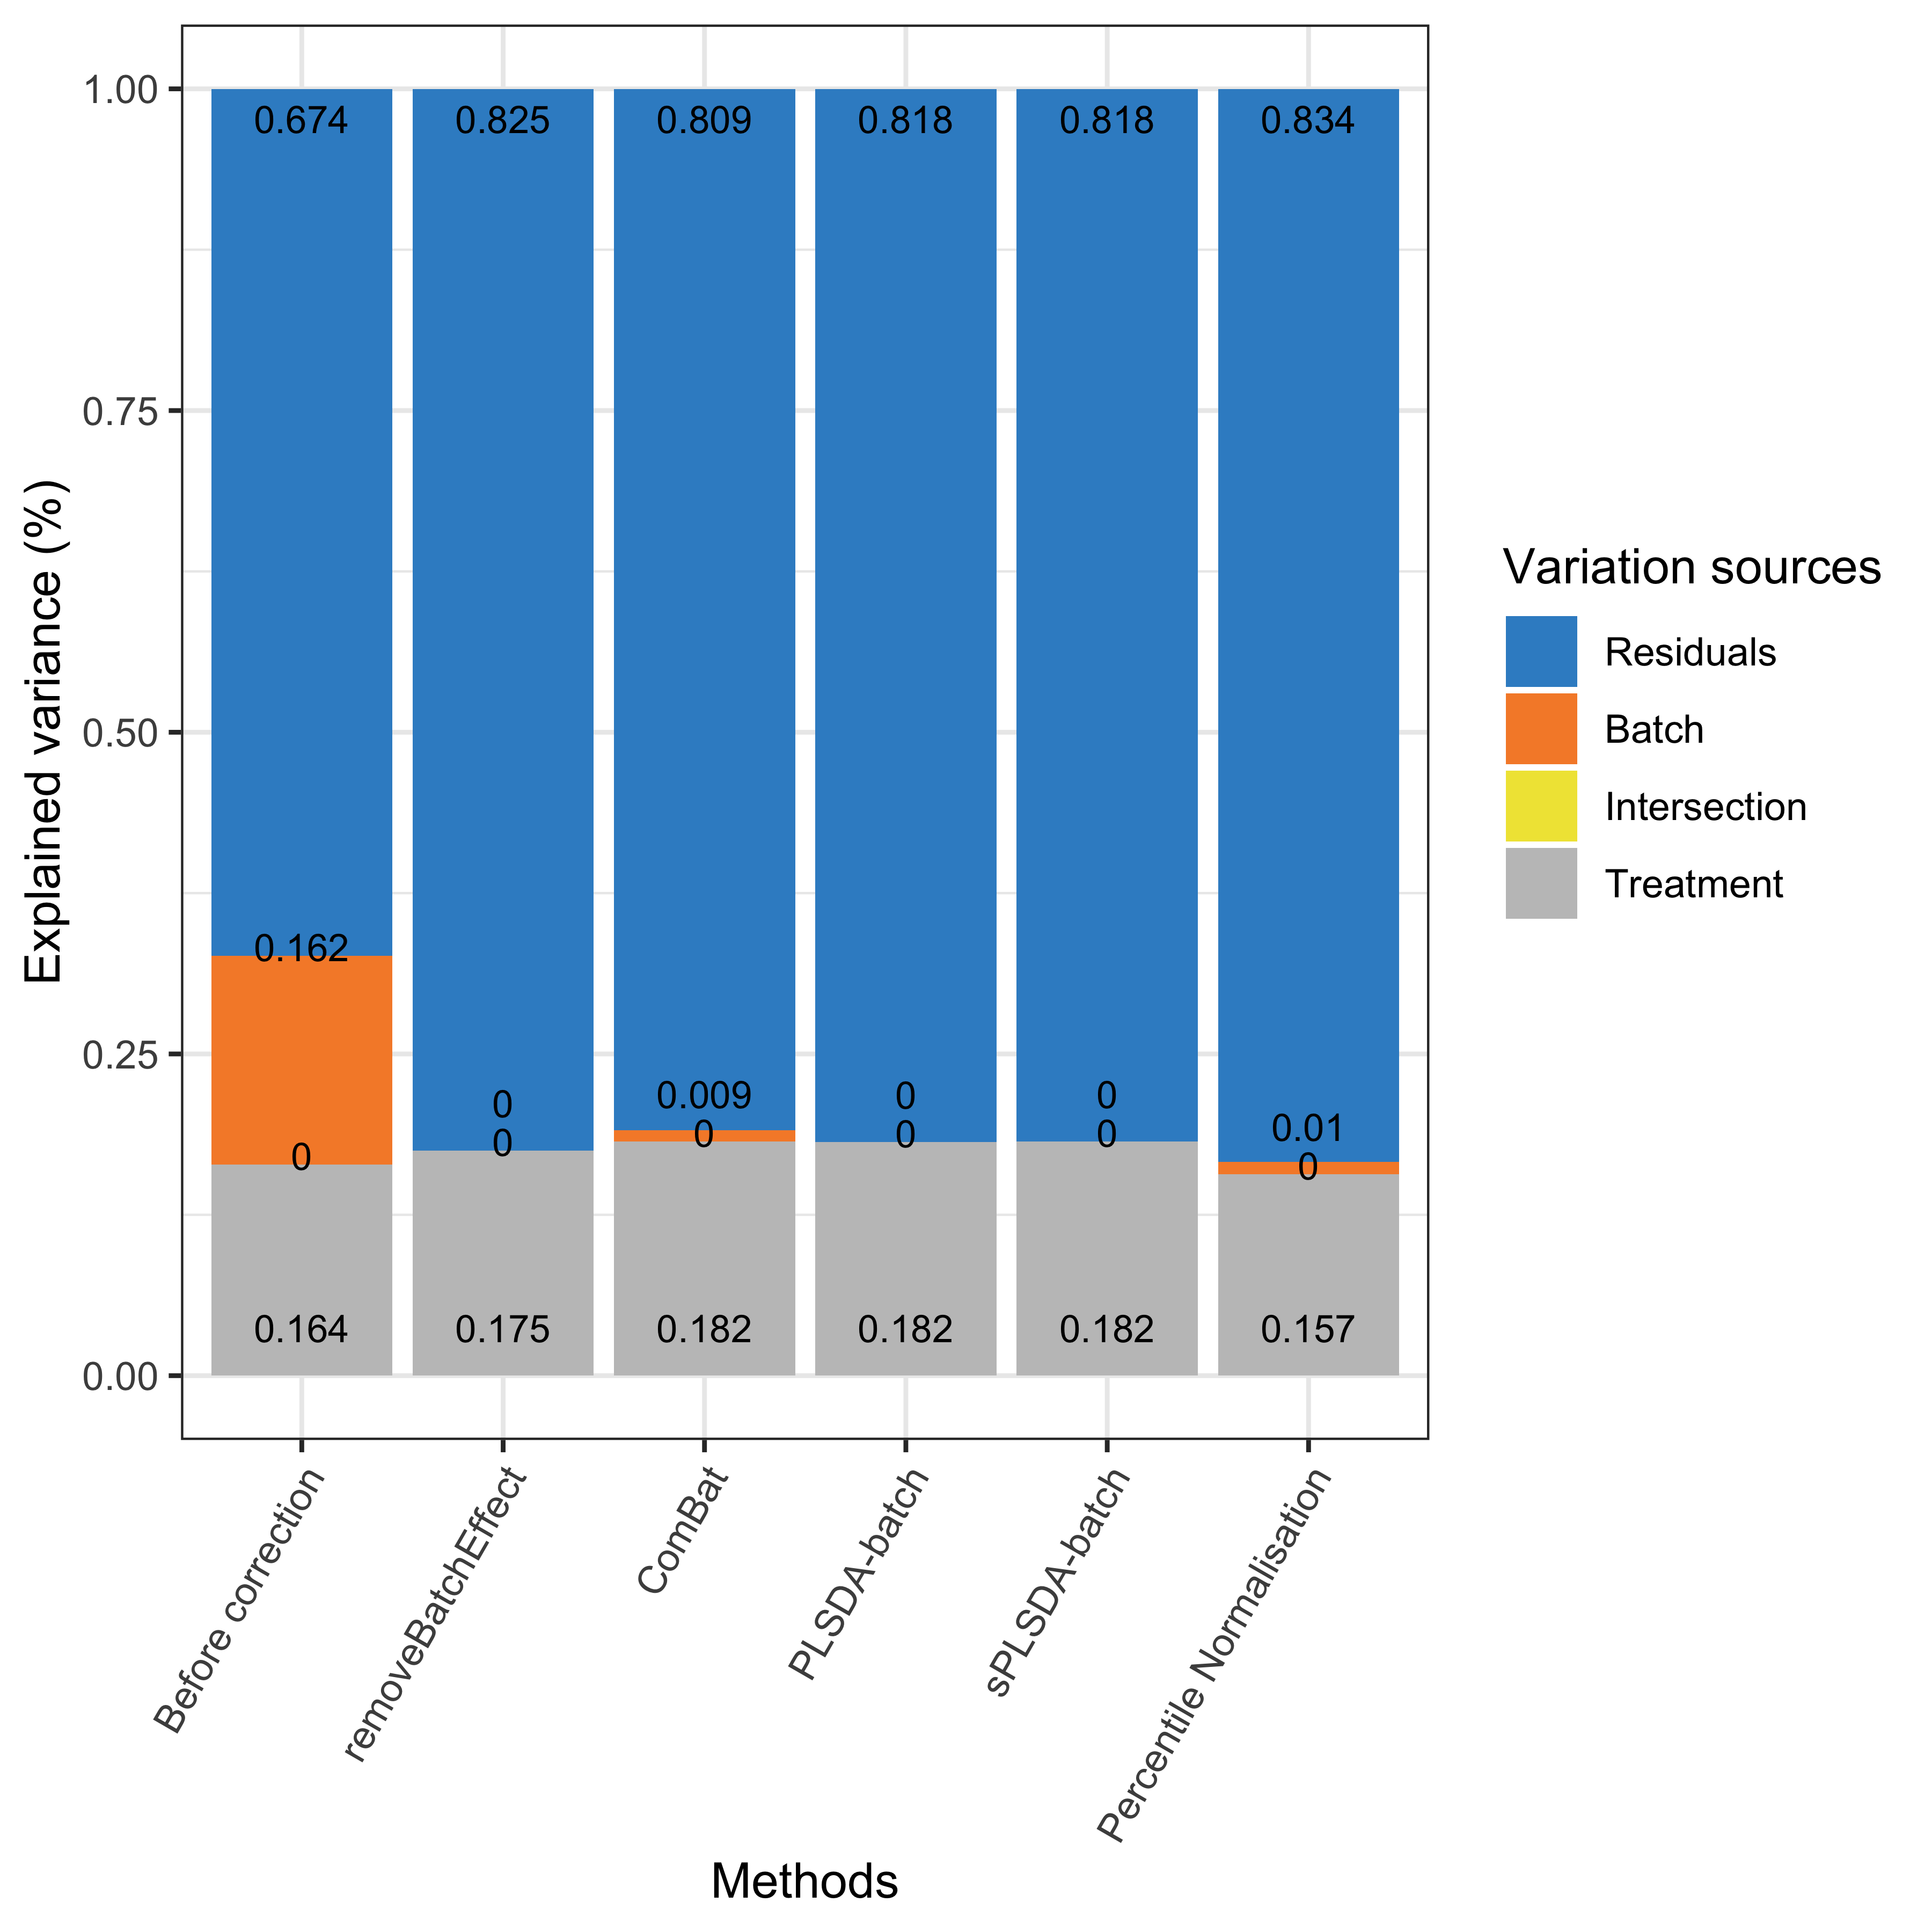
\includegraphics[width=0.6\linewidth]{PLSDAbatch_workflow_files/figure-latex/Spongeprda-1} 

}

\caption{Global explained variance before and after batch effect correction for the sponge data.}\label{fig:Spongeprda}
\end{figure}

As shown in the above figure, the intersection between batch and treatment variance was none for the \textcolor{brown}{sponge data}, because the batch x treatment design is balanced. PLSDA-batch and sPLSDA-batch corrected data led to the best performance with a slightly higher proportion of explained treatment variance and no batch variance compared to the other methods.

\hypertarget{other-methods}{%
\subsubsection{Other methods}\label{other-methods}}

\(\mathbf{R^2}\)

The \(R^2\) values for each variable are calculated with \texttt{lm()} from \textcolor{orange}{stats} package. To compare the \(R^2\) values among variables, we scale the corrected data before \(R^2\) calculation. The results are displayed with \texttt{ggplot()} from \textcolor{orange}{ggplot2} R package.

\begin{Shaded}
\begin{Highlighting}[]
\CommentTok{\# scale}
\NormalTok{sponge.corr\_scale.list }\OtherTok{\textless{}{-}} \FunctionTok{lapply}\NormalTok{(sponge.corrected.list, }
                                 \ControlFlowTok{function}\NormalTok{(x)\{}\FunctionTok{apply}\NormalTok{(x, }\DecValTok{2}\NormalTok{, scale)\})}

\NormalTok{sponge.r\_values.list }\OtherTok{\textless{}{-}} \FunctionTok{list}\NormalTok{()}
\ControlFlowTok{for}\NormalTok{(i }\ControlFlowTok{in} \DecValTok{1}\SpecialCharTok{:}\FunctionTok{length}\NormalTok{(sponge.corr\_scale.list))\{}
\NormalTok{  sponge.r\_values }\OtherTok{\textless{}{-}} \FunctionTok{data.frame}\NormalTok{(}\AttributeTok{trt =} \ConstantTok{NA}\NormalTok{, }\AttributeTok{batch =} \ConstantTok{NA}\NormalTok{)}
  \ControlFlowTok{for}\NormalTok{(c }\ControlFlowTok{in} \DecValTok{1}\SpecialCharTok{:}\FunctionTok{ncol}\NormalTok{(sponge.corr\_scale.list[[i]]))\{}
\NormalTok{    sponge.fit.res.trt }\OtherTok{\textless{}{-}} \FunctionTok{lm}\NormalTok{(sponge.corr\_scale.list[[i]][,c] }\SpecialCharTok{\textasciitilde{}}\NormalTok{ sponge.trt)}
\NormalTok{    sponge.r\_values[c,}\DecValTok{1}\NormalTok{] }\OtherTok{\textless{}{-}} \FunctionTok{summary}\NormalTok{(sponge.fit.res.trt)}\SpecialCharTok{$}\NormalTok{r.squared}
\NormalTok{    sponge.fit.res.batch }\OtherTok{\textless{}{-}} \FunctionTok{lm}\NormalTok{(sponge.corr\_scale.list[[i]][,c] }\SpecialCharTok{\textasciitilde{}}\NormalTok{ sponge.batch)}
\NormalTok{    sponge.r\_values[c,}\DecValTok{2}\NormalTok{] }\OtherTok{\textless{}{-}} \FunctionTok{summary}\NormalTok{(sponge.fit.res.batch)}\SpecialCharTok{$}\NormalTok{r.squared}
\NormalTok{  \}}
\NormalTok{  sponge.r\_values.list[[i]] }\OtherTok{\textless{}{-}}\NormalTok{ sponge.r\_values}
\NormalTok{\}}
\FunctionTok{names}\NormalTok{(sponge.r\_values.list) }\OtherTok{\textless{}{-}} \FunctionTok{names}\NormalTok{(sponge.corr\_scale.list)}

\NormalTok{sponge.boxp.list }\OtherTok{\textless{}{-}} \FunctionTok{list}\NormalTok{()}
\ControlFlowTok{for}\NormalTok{(i }\ControlFlowTok{in} \FunctionTok{seq\_len}\NormalTok{(}\FunctionTok{length}\NormalTok{(sponge.r\_values.list)))\{}
\NormalTok{  sponge.boxp.list[[i]] }\OtherTok{\textless{}{-}} 
    \FunctionTok{data.frame}\NormalTok{(}\AttributeTok{r2 =} \FunctionTok{c}\NormalTok{(sponge.r\_values.list[[i]][ ,}\StringTok{\textquotesingle{}trt\textquotesingle{}}\NormalTok{],}
\NormalTok{                      sponge.r\_values.list[[i]][ ,}\StringTok{\textquotesingle{}batch\textquotesingle{}}\NormalTok{]), }
               \AttributeTok{Effects =} \FunctionTok{as.factor}\NormalTok{(}\FunctionTok{rep}\NormalTok{(}\FunctionTok{c}\NormalTok{(}\StringTok{\textquotesingle{}Treatment\textquotesingle{}}\NormalTok{,}\StringTok{\textquotesingle{}Batch\textquotesingle{}}\NormalTok{), }
                                       \AttributeTok{each =} \DecValTok{24}\NormalTok{)))}
\NormalTok{\}}
\FunctionTok{names}\NormalTok{(sponge.boxp.list) }\OtherTok{\textless{}{-}} \FunctionTok{names}\NormalTok{(sponge.r\_values.list)}

\NormalTok{sponge.r2.boxp }\OtherTok{\textless{}{-}} \FunctionTok{rbind}\NormalTok{(sponge.boxp.list}\SpecialCharTok{$}\StringTok{\textasciigrave{}}\AttributeTok{Before correction}\StringTok{\textasciigrave{}}\NormalTok{,}
\NormalTok{                        sponge.boxp.list}\SpecialCharTok{$}\NormalTok{removeBatchEffect,}
\NormalTok{                        sponge.boxp.list}\SpecialCharTok{$}\NormalTok{ComBat,}
\NormalTok{                        sponge.boxp.list}\SpecialCharTok{$}\StringTok{\textasciigrave{}}\AttributeTok{PLSDA{-}batch}\StringTok{\textasciigrave{}}\NormalTok{,}
\NormalTok{                        sponge.boxp.list}\SpecialCharTok{$}\StringTok{\textasciigrave{}}\AttributeTok{sPLSDA{-}batch}\StringTok{\textasciigrave{}}\NormalTok{,}
\NormalTok{                        sponge.boxp.list}\SpecialCharTok{$}\StringTok{\textasciigrave{}}\AttributeTok{Percentile Normalisation}\StringTok{\textasciigrave{}}\NormalTok{,}
\NormalTok{                        sponge.boxp.list}\SpecialCharTok{$}\NormalTok{RUVIII)}

\NormalTok{sponge.r2.boxp}\SpecialCharTok{$}\NormalTok{methods }\OtherTok{\textless{}{-}} \FunctionTok{rep}\NormalTok{(}\FunctionTok{c}\NormalTok{(}\StringTok{\textquotesingle{}Before correction\textquotesingle{}}\NormalTok{, }\StringTok{\textquotesingle{} removeBatchEffect\textquotesingle{}}\NormalTok{, }
                                \StringTok{\textquotesingle{}ComBat\textquotesingle{}}\NormalTok{,}\StringTok{\textquotesingle{}PLSDA{-}batch\textquotesingle{}}\NormalTok{, }\StringTok{\textquotesingle{}sPLSDA{-}batch\textquotesingle{}}\NormalTok{,}
                                \StringTok{\textquotesingle{}Percentile Normalisation\textquotesingle{}}\NormalTok{), }\AttributeTok{each =} \DecValTok{48}\NormalTok{)}

\NormalTok{sponge.r2.boxp}\SpecialCharTok{$}\NormalTok{methods }\OtherTok{\textless{}{-}} \FunctionTok{factor}\NormalTok{(sponge.r2.boxp}\SpecialCharTok{$}\NormalTok{methods, }
                                 \AttributeTok{levels =} \FunctionTok{unique}\NormalTok{(sponge.r2.boxp}\SpecialCharTok{$}\NormalTok{methods))}

\FunctionTok{ggplot}\NormalTok{(sponge.r2.boxp, }\FunctionTok{aes}\NormalTok{(}\AttributeTok{x =}\NormalTok{ Effects, }\AttributeTok{y =}\NormalTok{ r2, }\AttributeTok{fill =}\NormalTok{ Effects)) }\SpecialCharTok{+}
  \FunctionTok{geom\_boxplot}\NormalTok{(}\AttributeTok{alpha =} \FloatTok{0.80}\NormalTok{) }\SpecialCharTok{+}
  \FunctionTok{theme\_bw}\NormalTok{() }\SpecialCharTok{+} 
  \FunctionTok{theme}\NormalTok{(}\AttributeTok{text =} \FunctionTok{element\_text}\NormalTok{(}\AttributeTok{size =} \DecValTok{18}\NormalTok{),}
        \AttributeTok{axis.title.x =} \FunctionTok{element\_blank}\NormalTok{(),}
        \AttributeTok{axis.title.y =} \FunctionTok{element\_blank}\NormalTok{(),}
        \AttributeTok{axis.text.x =} \FunctionTok{element\_text}\NormalTok{(}\AttributeTok{angle =} \DecValTok{60}\NormalTok{, }\AttributeTok{hjust =} \DecValTok{1}\NormalTok{, }\AttributeTok{size =} \DecValTok{18}\NormalTok{),}
        \AttributeTok{axis.text.y =} \FunctionTok{element\_text}\NormalTok{(}\AttributeTok{size =} \DecValTok{18}\NormalTok{),}
        \AttributeTok{panel.grid.minor.x =} \FunctionTok{element\_blank}\NormalTok{(),}
        \AttributeTok{panel.grid.major.x =} \FunctionTok{element\_blank}\NormalTok{(),}
        \AttributeTok{legend.position =} \StringTok{"right"}\NormalTok{) }\SpecialCharTok{+} \FunctionTok{facet\_grid}\NormalTok{( }\SpecialCharTok{\textasciitilde{}}\NormalTok{ methods) }\SpecialCharTok{+} 
  \FunctionTok{scale\_fill\_manual}\NormalTok{(}\AttributeTok{values=}\FunctionTok{pb\_color}\NormalTok{(}\FunctionTok{c}\NormalTok{(}\DecValTok{12}\NormalTok{,}\DecValTok{14}\NormalTok{))) }
\end{Highlighting}
\end{Shaded}

\begin{figure}

{\centering 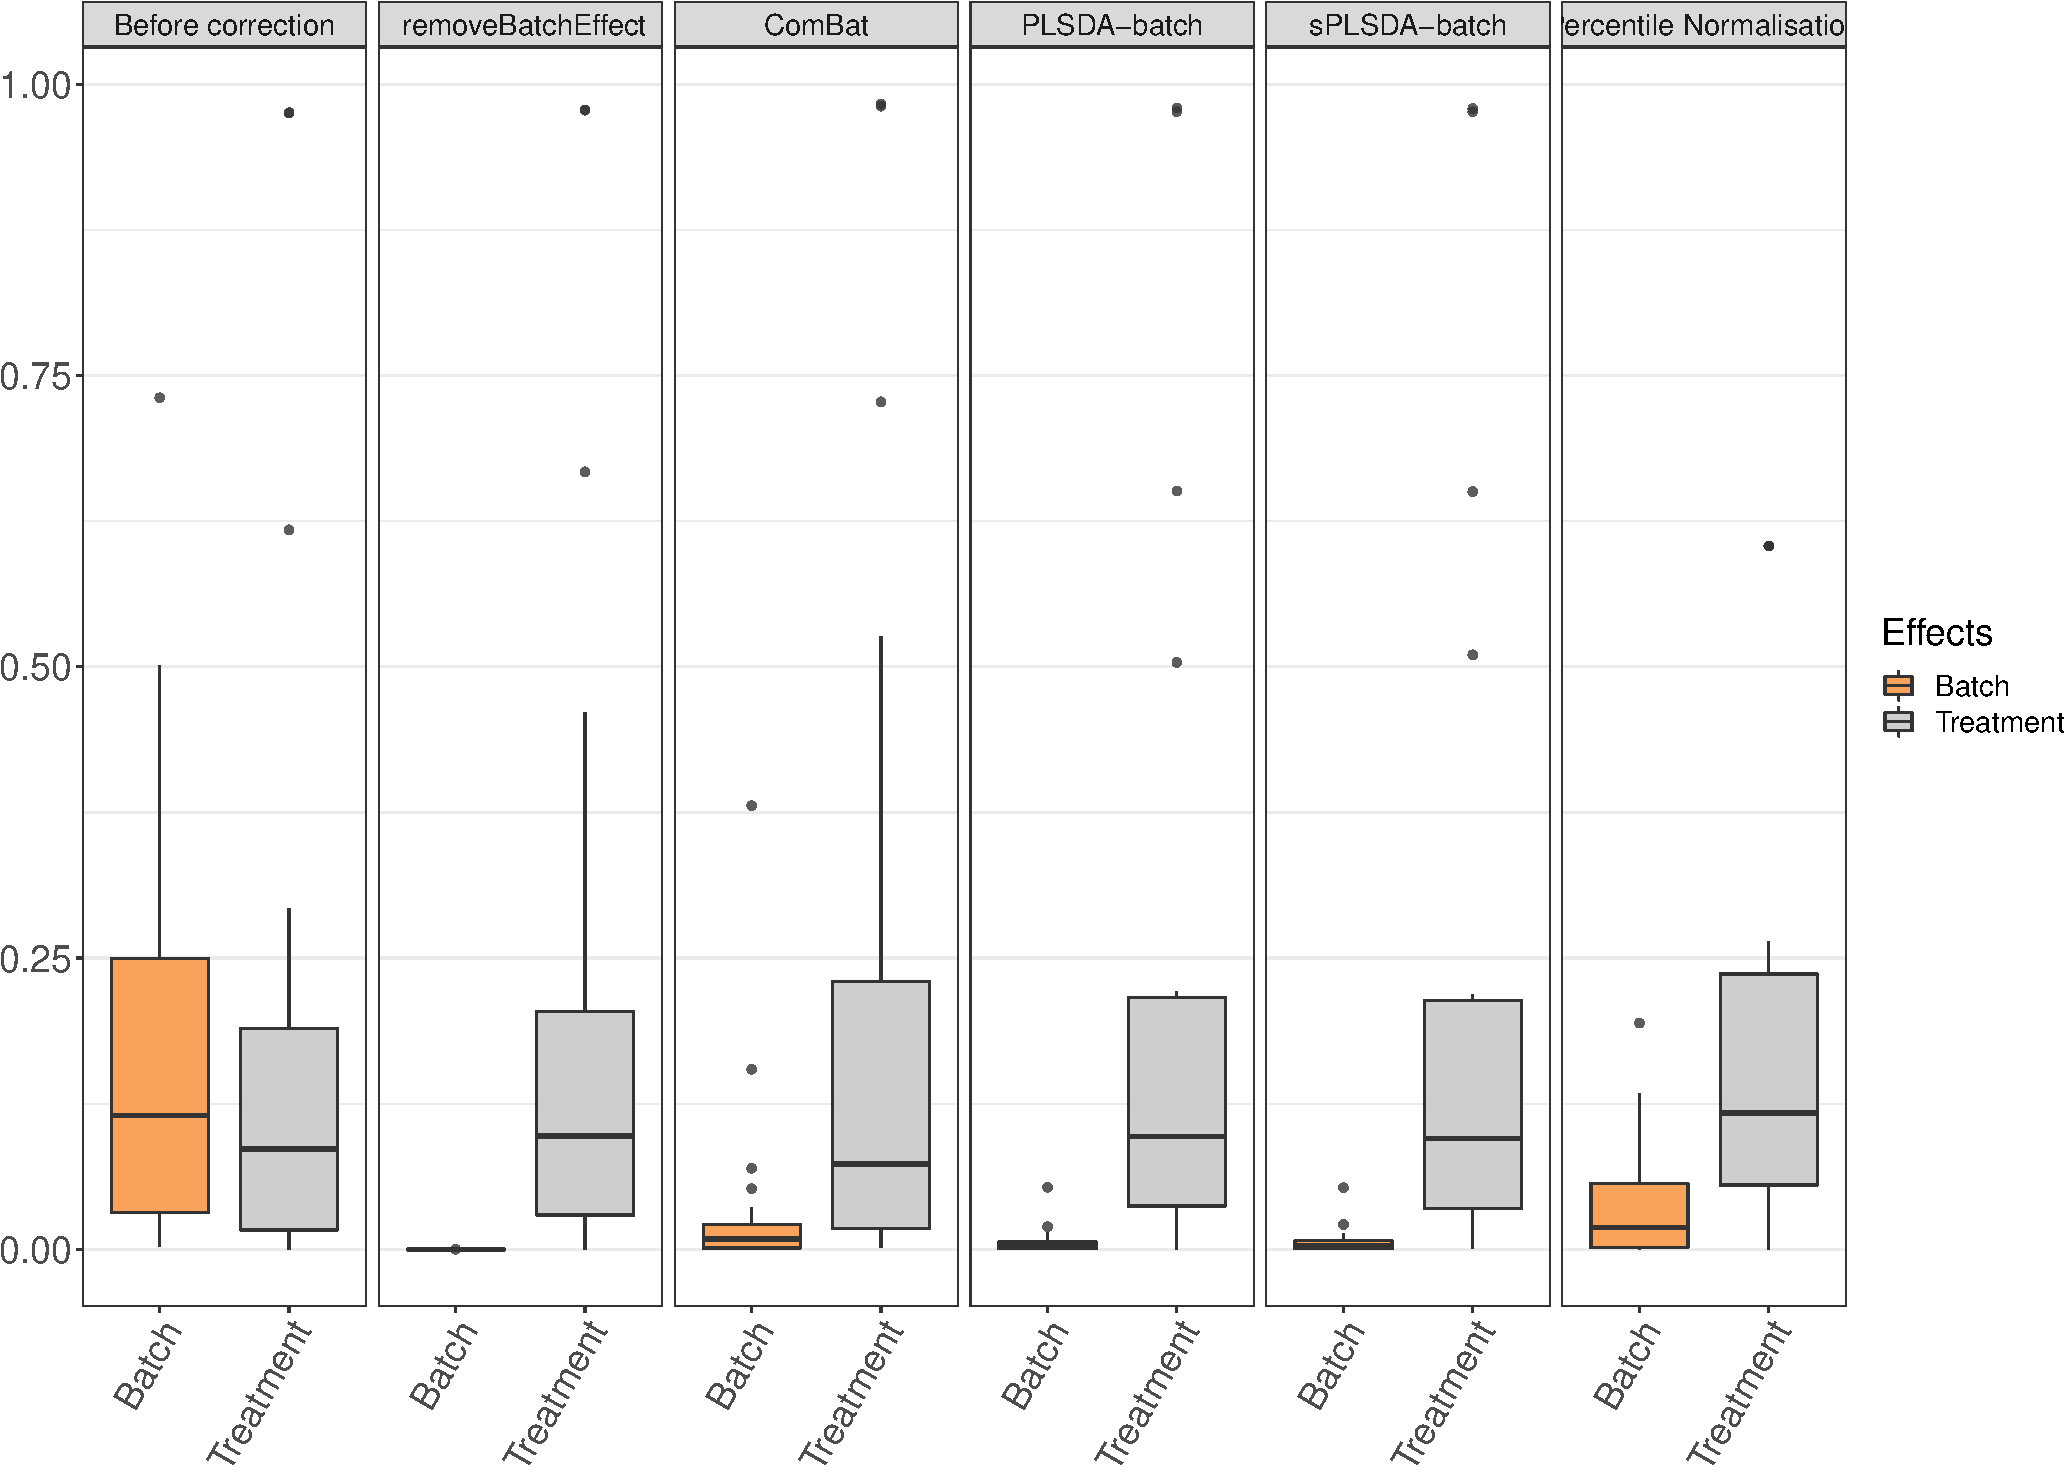
\includegraphics[width=1\linewidth]{PLSDAbatch_workflow_files/figure-latex/Sponger21-1} 

}

\caption{Sponge study: $R^2$ values for each microbial variable before and after batch effect correction.}\label{fig:Sponger21}
\end{figure}

We observed that the data corrected by ComBat, percentile normalisation still included a few variables with a large proportion of batch variance as shown in the above figures.

\begin{Shaded}
\begin{Highlighting}[]
\DocumentationTok{\#\#\#\#\#\#\#\#\#\#\#\#\#\#\#\#\#\#\#\#\#\#\#\#\#\#\#\#\#\#\#\#\#\#}
\NormalTok{sponge.barp.list }\OtherTok{\textless{}{-}} \FunctionTok{list}\NormalTok{()}
\ControlFlowTok{for}\NormalTok{(i }\ControlFlowTok{in} \FunctionTok{seq\_len}\NormalTok{(}\FunctionTok{length}\NormalTok{(sponge.r\_values.list)))\{}
\NormalTok{  sponge.barp.list[[i]] }\OtherTok{\textless{}{-}} 
    \FunctionTok{data.frame}\NormalTok{(}\AttributeTok{r2 =} \FunctionTok{c}\NormalTok{(}\FunctionTok{sum}\NormalTok{(sponge.r\_values.list[[i]][ ,}\StringTok{\textquotesingle{}trt\textquotesingle{}}\NormalTok{]),}
                      \FunctionTok{sum}\NormalTok{(sponge.r\_values.list[[i]][ ,}\StringTok{\textquotesingle{}batch\textquotesingle{}}\NormalTok{])), }
               \AttributeTok{Effects =} \FunctionTok{c}\NormalTok{(}\StringTok{\textquotesingle{}Treatment\textquotesingle{}}\NormalTok{,}\StringTok{\textquotesingle{}Batch\textquotesingle{}}\NormalTok{))}
\NormalTok{\}}
\FunctionTok{names}\NormalTok{(sponge.barp.list) }\OtherTok{\textless{}{-}} \FunctionTok{names}\NormalTok{(sponge.r\_values.list)}

\NormalTok{sponge.r2.barp }\OtherTok{\textless{}{-}} \FunctionTok{rbind}\NormalTok{(sponge.barp.list}\SpecialCharTok{$}\StringTok{\textasciigrave{}}\AttributeTok{Before correction}\StringTok{\textasciigrave{}}\NormalTok{,}
\NormalTok{                        sponge.barp.list}\SpecialCharTok{$}\NormalTok{removeBatchEffect,}
\NormalTok{                        sponge.barp.list}\SpecialCharTok{$}\NormalTok{ComBat,}
\NormalTok{                        sponge.barp.list}\SpecialCharTok{$}\StringTok{\textasciigrave{}}\AttributeTok{PLSDA{-}batch}\StringTok{\textasciigrave{}}\NormalTok{,}
\NormalTok{                        sponge.barp.list}\SpecialCharTok{$}\StringTok{\textasciigrave{}}\AttributeTok{sPLSDA{-}batch}\StringTok{\textasciigrave{}}\NormalTok{,}
\NormalTok{                        sponge.barp.list}\SpecialCharTok{$}\StringTok{\textasciigrave{}}\AttributeTok{Percentile Normalisation}\StringTok{\textasciigrave{}}\NormalTok{,}
\NormalTok{                        sponge.barp.list}\SpecialCharTok{$}\NormalTok{RUVIII)}


\NormalTok{sponge.r2.barp}\SpecialCharTok{$}\NormalTok{methods }\OtherTok{\textless{}{-}} \FunctionTok{rep}\NormalTok{(}\FunctionTok{c}\NormalTok{(}\StringTok{\textquotesingle{}Before correction\textquotesingle{}}\NormalTok{, }\StringTok{\textquotesingle{} removeBatchEffect\textquotesingle{}}\NormalTok{, }
                                \StringTok{\textquotesingle{}ComBat\textquotesingle{}}\NormalTok{,}\StringTok{\textquotesingle{}PLSDA{-}batch\textquotesingle{}}\NormalTok{, }\StringTok{\textquotesingle{}sPLSDA{-}batch\textquotesingle{}}\NormalTok{,}
                                \StringTok{\textquotesingle{}Percentile Normalisation\textquotesingle{}}\NormalTok{), }\AttributeTok{each =} \DecValTok{2}\NormalTok{)}

\NormalTok{sponge.r2.barp}\SpecialCharTok{$}\NormalTok{methods }\OtherTok{\textless{}{-}} \FunctionTok{factor}\NormalTok{(sponge.r2.barp}\SpecialCharTok{$}\NormalTok{methods, }
                                 \AttributeTok{levels =} \FunctionTok{unique}\NormalTok{(sponge.r2.barp}\SpecialCharTok{$}\NormalTok{methods))}


\FunctionTok{ggplot}\NormalTok{(sponge.r2.barp, }\FunctionTok{aes}\NormalTok{(}\AttributeTok{x =}\NormalTok{ Effects, }\AttributeTok{y =}\NormalTok{ r2, }\AttributeTok{fill =}\NormalTok{ Effects)) }\SpecialCharTok{+}
  \FunctionTok{geom\_bar}\NormalTok{(}\AttributeTok{stat=}\StringTok{"identity"}\NormalTok{) }\SpecialCharTok{+} 
  \FunctionTok{theme\_bw}\NormalTok{() }\SpecialCharTok{+} 
  \FunctionTok{theme}\NormalTok{(}\AttributeTok{text =} \FunctionTok{element\_text}\NormalTok{(}\AttributeTok{size =} \DecValTok{18}\NormalTok{),}
        \AttributeTok{axis.title.x =} \FunctionTok{element\_blank}\NormalTok{(),}
        \AttributeTok{axis.title.y =} \FunctionTok{element\_blank}\NormalTok{(),}
        \AttributeTok{axis.text.x =} \FunctionTok{element\_text}\NormalTok{(}\AttributeTok{angle =} \DecValTok{60}\NormalTok{, }\AttributeTok{hjust =} \DecValTok{1}\NormalTok{, }\AttributeTok{size =} \DecValTok{18}\NormalTok{),}
        \AttributeTok{axis.text.y =} \FunctionTok{element\_text}\NormalTok{(}\AttributeTok{size =} \DecValTok{18}\NormalTok{),}
        \AttributeTok{panel.grid.minor.x =} \FunctionTok{element\_blank}\NormalTok{(),}
        \AttributeTok{panel.grid.major.x =} \FunctionTok{element\_blank}\NormalTok{(),}
        \AttributeTok{legend.position =} \StringTok{"right"}\NormalTok{) }\SpecialCharTok{+} \FunctionTok{facet\_grid}\NormalTok{( }\SpecialCharTok{\textasciitilde{}}\NormalTok{ methods) }\SpecialCharTok{+} 
  \FunctionTok{scale\_fill\_manual}\NormalTok{(}\AttributeTok{values=}\FunctionTok{pb\_color}\NormalTok{(}\FunctionTok{c}\NormalTok{(}\DecValTok{12}\NormalTok{,}\DecValTok{14}\NormalTok{)))}
\end{Highlighting}
\end{Shaded}

\begin{figure}

{\centering \includegraphics[width=1\linewidth]{PLSDAbatch_workflow_files/figure-latex/Sponger22-1} 

}

\caption{Sponge study: the sum of $R^2$ values for each microbial variable before and after batch effect correction.}\label{fig:Sponger22}
\end{figure}

When considering the sum of all variables, the remaining batch variance of corrected data from sPLSDA-batch was similar as PLSDA-batch, which was greater than removeBatchEffect. The preserved treatment variance of corrected data from sPLSDA-batch was also similar as PLSDA-batch which was greater than removeBatchEffect.

\textbf{Alignment scores}

To use the \texttt{alignment\_score()} function from \textcolor{orange}{PLSDAbatch}, we need to specify the proportion of data variance to explain (\texttt{var}), the number of nearest neighbours (\texttt{k}) and the number of principal components to estimate (\texttt{ncomp}). We then use \texttt{ggplot()} function from \textcolor{orange}{ggplot2} to visualise the results.

\begin{Shaded}
\begin{Highlighting}[]
\NormalTok{sponge.var }\OtherTok{=} \FloatTok{0.95}
\NormalTok{sponge.k }\OtherTok{=} \DecValTok{3}

\NormalTok{sponge.scores }\OtherTok{\textless{}{-}} \FunctionTok{c}\NormalTok{()}
\ControlFlowTok{for}\NormalTok{(i }\ControlFlowTok{in} \DecValTok{1}\SpecialCharTok{:}\FunctionTok{length}\NormalTok{(sponge.corrected.list))\{}
\NormalTok{  res }\OtherTok{\textless{}{-}} \FunctionTok{alignment\_score}\NormalTok{(}\AttributeTok{data =}\NormalTok{ sponge.corrected.list[[i]], }
                         \AttributeTok{batch =}\NormalTok{ sponge.batch, }
                         \AttributeTok{var =}\NormalTok{ sponge.var, }
                         \AttributeTok{k =}\NormalTok{ sponge.k, }
                         \AttributeTok{ncomp =} \DecValTok{20}\NormalTok{)}
\NormalTok{  sponge.scores }\OtherTok{\textless{}{-}} \FunctionTok{c}\NormalTok{(sponge.scores, res)}
\NormalTok{\}}

\NormalTok{sponge.scores.df }\OtherTok{\textless{}{-}} \FunctionTok{data.frame}\NormalTok{(}\AttributeTok{scores =}\NormalTok{ sponge.scores, }
                               \AttributeTok{methods =} \FunctionTok{names}\NormalTok{(sponge.corrected.list))}

\NormalTok{sponge.scores.df}\SpecialCharTok{$}\NormalTok{methods }\OtherTok{\textless{}{-}} \FunctionTok{factor}\NormalTok{(sponge.scores.df}\SpecialCharTok{$}\NormalTok{methods, }
                                   \AttributeTok{levels =} \FunctionTok{rev}\NormalTok{(}\FunctionTok{names}\NormalTok{(sponge.corrected.list)))}


\FunctionTok{ggplot}\NormalTok{() }\SpecialCharTok{+} \FunctionTok{geom\_col}\NormalTok{(}\FunctionTok{aes}\NormalTok{(}\AttributeTok{x =}\NormalTok{ sponge.scores.df}\SpecialCharTok{$}\NormalTok{methods, }
                        \AttributeTok{y =}\NormalTok{ sponge.scores.df}\SpecialCharTok{$}\NormalTok{scores)) }\SpecialCharTok{+} 
  \FunctionTok{geom\_text}\NormalTok{(}\FunctionTok{aes}\NormalTok{(}\AttributeTok{x =}\NormalTok{ sponge.scores.df}\SpecialCharTok{$}\NormalTok{methods, }
                \AttributeTok{y =}\NormalTok{ sponge.scores.df}\SpecialCharTok{$}\NormalTok{scores}\SpecialCharTok{/}\DecValTok{2}\NormalTok{, }
                \AttributeTok{label =} \FunctionTok{round}\NormalTok{(sponge.scores.df}\SpecialCharTok{$}\NormalTok{scores, }\DecValTok{3}\NormalTok{)), }
            \AttributeTok{size =} \DecValTok{3}\NormalTok{, }\AttributeTok{col =} \StringTok{\textquotesingle{}white\textquotesingle{}}\NormalTok{) }\SpecialCharTok{+} 
  \FunctionTok{coord\_flip}\NormalTok{() }\SpecialCharTok{+} \FunctionTok{theme\_bw}\NormalTok{() }\SpecialCharTok{+} \FunctionTok{ylab}\NormalTok{(}\StringTok{\textquotesingle{}Alignment Scores\textquotesingle{}}\NormalTok{) }\SpecialCharTok{+} 
  \FunctionTok{xlab}\NormalTok{(}\StringTok{\textquotesingle{}\textquotesingle{}}\NormalTok{) }\SpecialCharTok{+} \FunctionTok{ylim}\NormalTok{(}\DecValTok{0}\NormalTok{,}\FloatTok{0.4}\NormalTok{)}
\end{Highlighting}
\end{Shaded}

\begin{figure}

{\centering 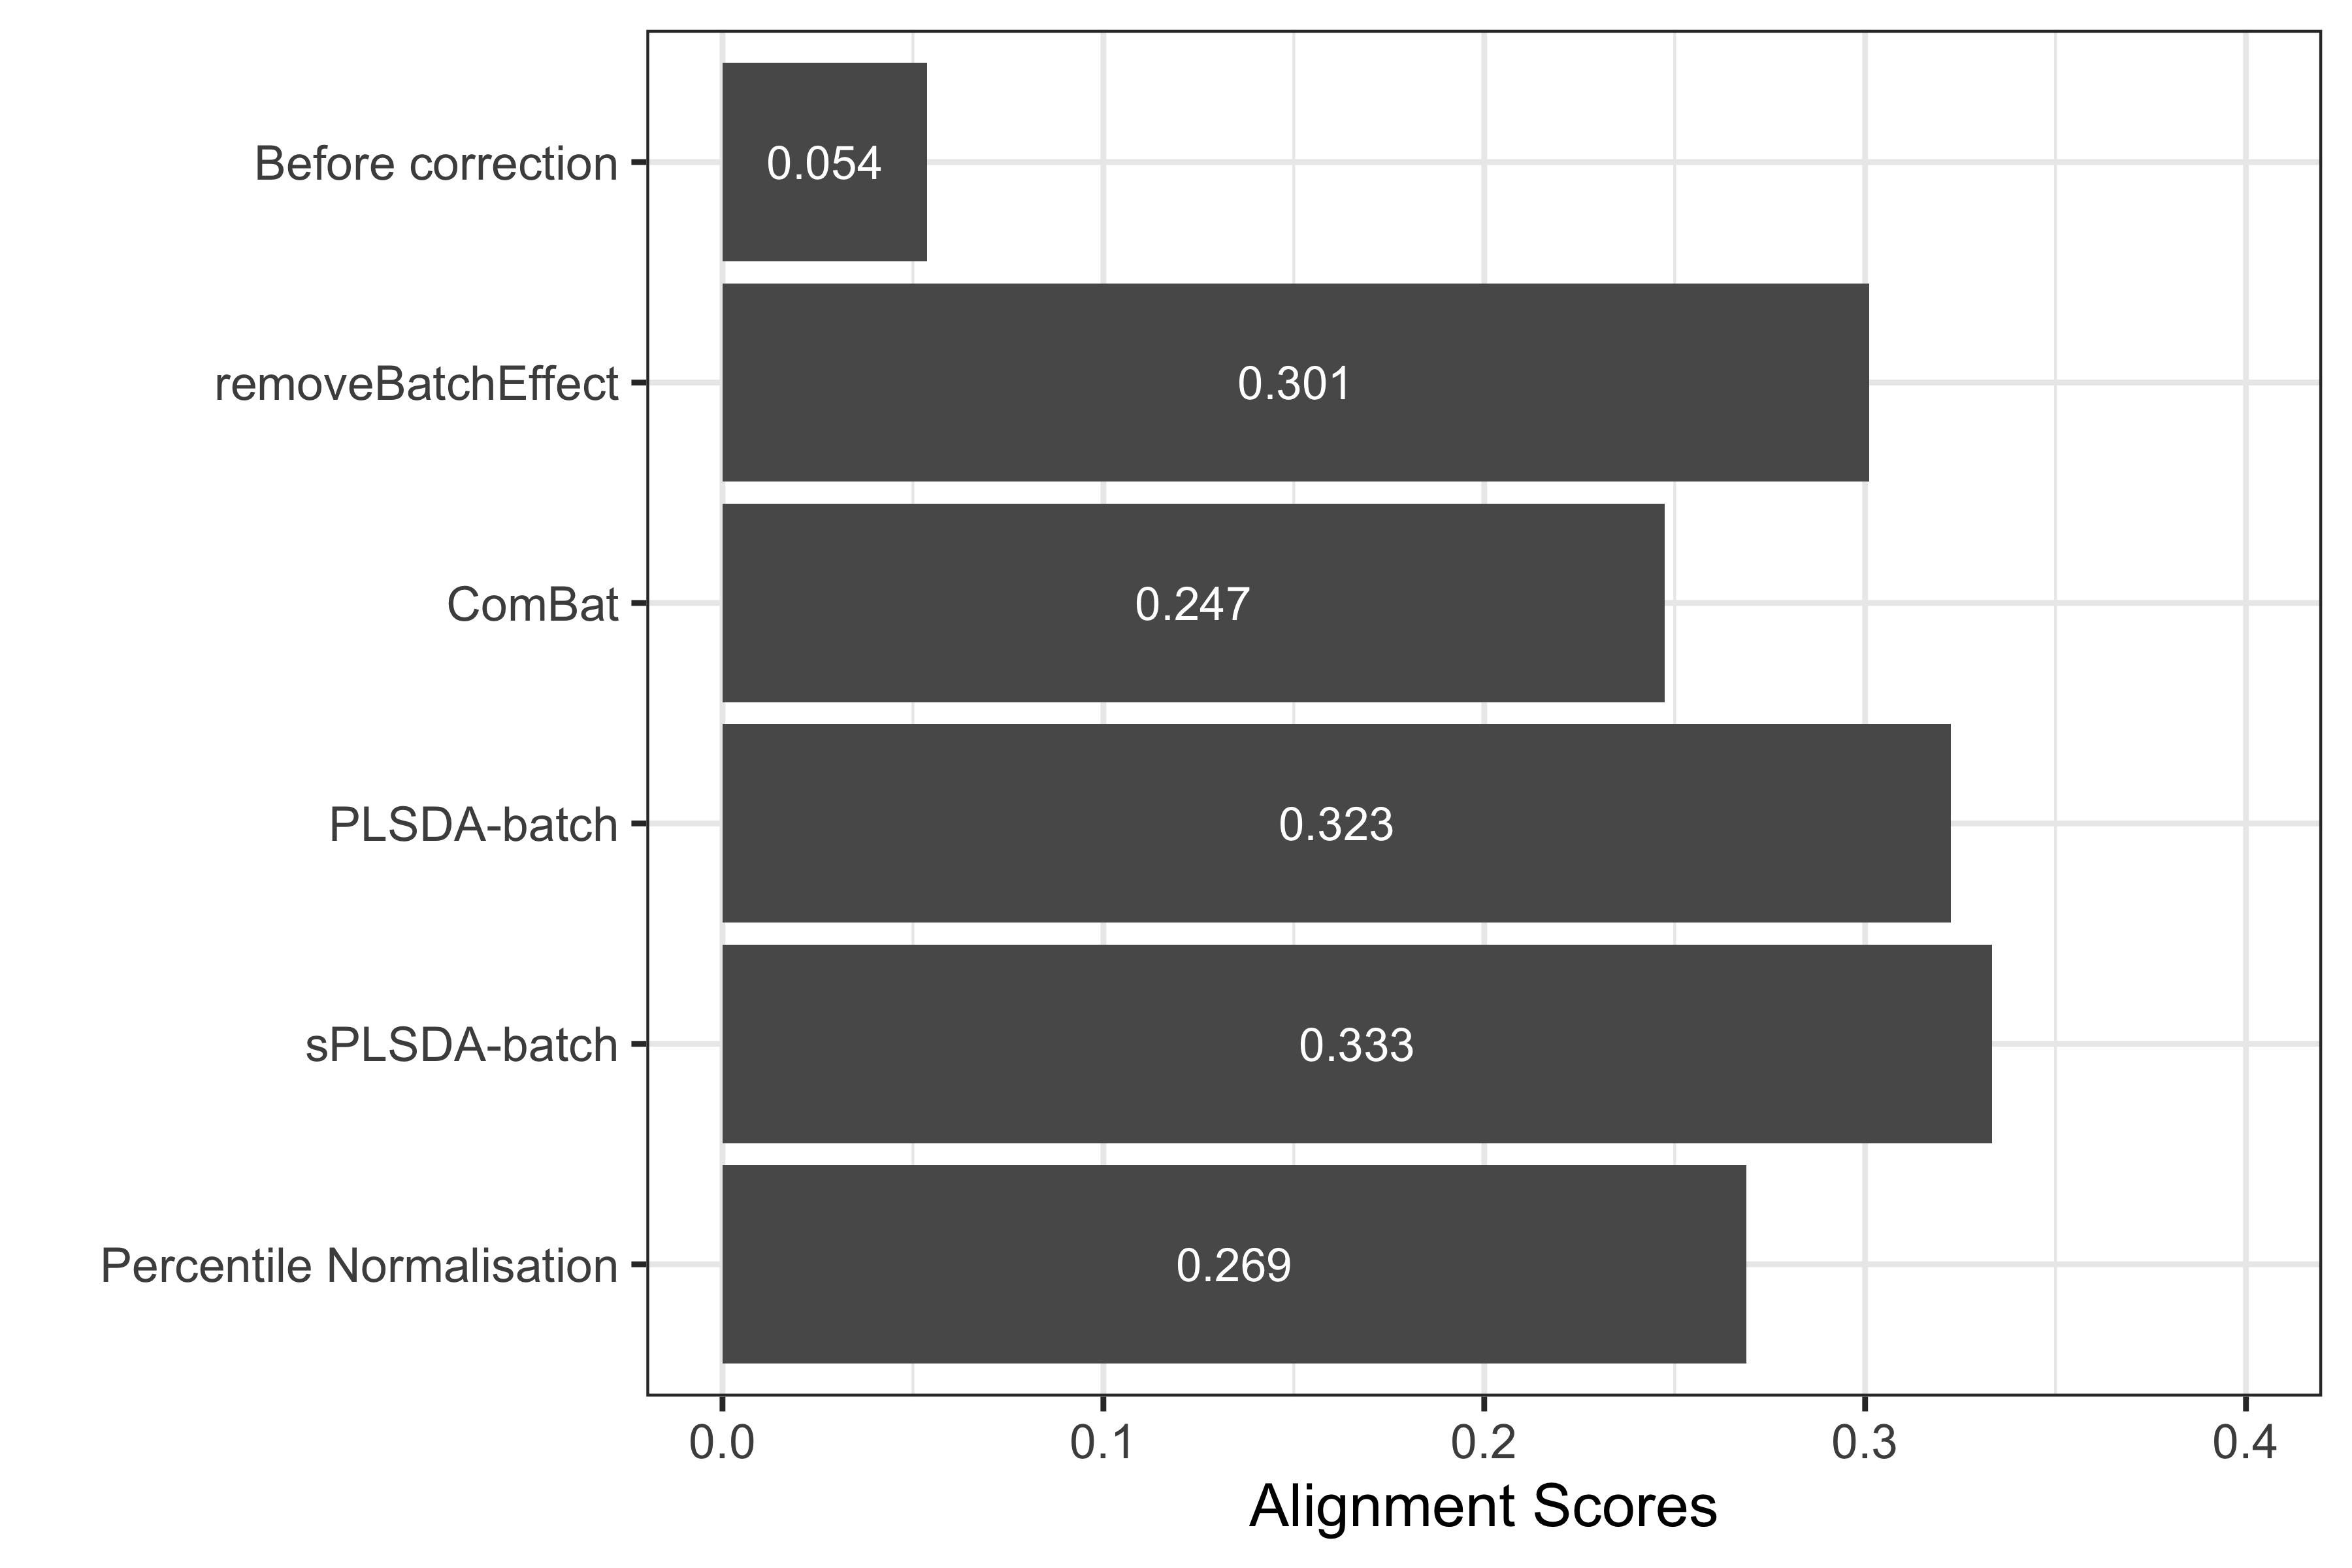
\includegraphics[width=0.6\linewidth]{PLSDAbatch_workflow_files/figure-latex/Spongealignment-1} 

}

\caption{Comparison of alignment scores before and after batch effect correction using different methods for the sponge data.}\label{fig:Spongealignment}
\end{figure}

The alignment scores complement the PCA results, especially when batch effect removal is difficult to assess on PCA sample plots. Since a higher alignment score indicates that samples are better mixed, as shown in the above figure, sPLSDA-batch gave a superior performance compared to the other methods.

\textbf{Variable selection}

We use \texttt{splsda()} from \textcolor{orange}{mixOmics} to select the top 5 microbial variables that, in combination, discriminate the different treatment groups in the \textcolor{brown}{sponge data}. We apply \texttt{splsda()} to the different batch effect corrected data from all methods. Then we use \texttt{upset()} from \textcolor{orange}{UpSetR} package \citep{lex2014upset} to visualise the concordance of variables selected.

In the code below, we first need to convert the list of variables selected from different method-corrected data into a data frame compatible with \texttt{upset()} using \texttt{fromList()}. We then assign different colour schemes for each variable selection.

\begin{Shaded}
\begin{Highlighting}[]
\NormalTok{sponge.splsda.select }\OtherTok{\textless{}{-}} \FunctionTok{list}\NormalTok{()}
\ControlFlowTok{for}\NormalTok{(i }\ControlFlowTok{in} \DecValTok{1}\SpecialCharTok{:}\FunctionTok{length}\NormalTok{(sponge.corrected.list))\{}
\NormalTok{  splsda.res }\OtherTok{\textless{}{-}} \FunctionTok{splsda}\NormalTok{(}\AttributeTok{X =}\NormalTok{ sponge.corrected.list[[i]], }
                       \AttributeTok{Y =}\NormalTok{ sponge.trt, }
                       \AttributeTok{ncomp =} \DecValTok{3}\NormalTok{, }\AttributeTok{keepX =} \FunctionTok{rep}\NormalTok{(}\DecValTok{5}\NormalTok{,}\DecValTok{3}\NormalTok{))}
\NormalTok{  select.res }\OtherTok{\textless{}{-}} \FunctionTok{selectVar}\NormalTok{(splsda.res, }\AttributeTok{comp =} \DecValTok{1}\NormalTok{)}\SpecialCharTok{$}\NormalTok{name}
\NormalTok{  sponge.splsda.select[[i]] }\OtherTok{\textless{}{-}}\NormalTok{ select.res}
\NormalTok{\}}
\FunctionTok{names}\NormalTok{(sponge.splsda.select) }\OtherTok{\textless{}{-}} \FunctionTok{names}\NormalTok{(sponge.corrected.list)}

\CommentTok{\# can only visualise 5 methods}
\NormalTok{sponge.splsda.select }\OtherTok{\textless{}{-}}\NormalTok{ sponge.splsda.select[}\FunctionTok{c}\NormalTok{(}\DecValTok{1}\SpecialCharTok{:}\DecValTok{5}\NormalTok{)]}

\NormalTok{sponge.splsda.upsetR }\OtherTok{\textless{}{-}} \FunctionTok{fromList}\NormalTok{(sponge.splsda.select)}

\FunctionTok{upset}\NormalTok{(sponge.splsda.upsetR, }\AttributeTok{main.bar.color =} \StringTok{\textquotesingle{}gray36\textquotesingle{}}\NormalTok{,}
      \AttributeTok{sets.bar.color =} \FunctionTok{pb\_color}\NormalTok{(}\FunctionTok{c}\NormalTok{(}\DecValTok{25}\SpecialCharTok{:}\DecValTok{22}\NormalTok{,}\DecValTok{20}\NormalTok{)), }\AttributeTok{matrix.color =} \StringTok{\textquotesingle{}gray36\textquotesingle{}}\NormalTok{,}
      \AttributeTok{order.by =} \StringTok{\textquotesingle{}freq\textquotesingle{}}\NormalTok{, }\AttributeTok{empty.intersections =} \StringTok{\textquotesingle{}on\textquotesingle{}}\NormalTok{,}
      \AttributeTok{queries =} 
        \FunctionTok{list}\NormalTok{(}\FunctionTok{list}\NormalTok{(}\AttributeTok{query =}\NormalTok{ intersects, }\AttributeTok{params =} \FunctionTok{list}\NormalTok{(}\StringTok{\textquotesingle{}Before correction\textquotesingle{}}\NormalTok{), }
                  \AttributeTok{color =} \FunctionTok{pb\_color}\NormalTok{(}\DecValTok{20}\NormalTok{), }\AttributeTok{active =}\NormalTok{ T),}
             \FunctionTok{list}\NormalTok{(}\AttributeTok{query =}\NormalTok{ intersects, }\AttributeTok{params =} \FunctionTok{list}\NormalTok{(}\StringTok{\textquotesingle{}removeBatchEffect\textquotesingle{}}\NormalTok{), }
                  \AttributeTok{color =} \FunctionTok{pb\_color}\NormalTok{(}\DecValTok{22}\NormalTok{), }\AttributeTok{active =}\NormalTok{ T),}
             \FunctionTok{list}\NormalTok{(}\AttributeTok{query =}\NormalTok{ intersects, }\AttributeTok{params =} \FunctionTok{list}\NormalTok{(}\StringTok{\textquotesingle{}ComBat\textquotesingle{}}\NormalTok{), }
                  \AttributeTok{color =} \FunctionTok{pb\_color}\NormalTok{(}\DecValTok{23}\NormalTok{), }\AttributeTok{active =}\NormalTok{ T),}
             \FunctionTok{list}\NormalTok{(}\AttributeTok{query =}\NormalTok{ intersects, }\AttributeTok{params =} \FunctionTok{list}\NormalTok{(}\StringTok{\textquotesingle{}PLSDA{-}batch\textquotesingle{}}\NormalTok{), }
                  \AttributeTok{color =} \FunctionTok{pb\_color}\NormalTok{(}\DecValTok{24}\NormalTok{), }\AttributeTok{active =}\NormalTok{ T),}
             \FunctionTok{list}\NormalTok{(}\AttributeTok{query =}\NormalTok{ intersects, }\AttributeTok{params =} \FunctionTok{list}\NormalTok{(}\StringTok{\textquotesingle{}sPLSDA{-}batch\textquotesingle{}}\NormalTok{), }
                  \AttributeTok{color =} \FunctionTok{pb\_color}\NormalTok{(}\DecValTok{25}\NormalTok{), }\AttributeTok{active =}\NormalTok{ T)))}
\end{Highlighting}
\end{Shaded}

\begin{figure}

{\centering 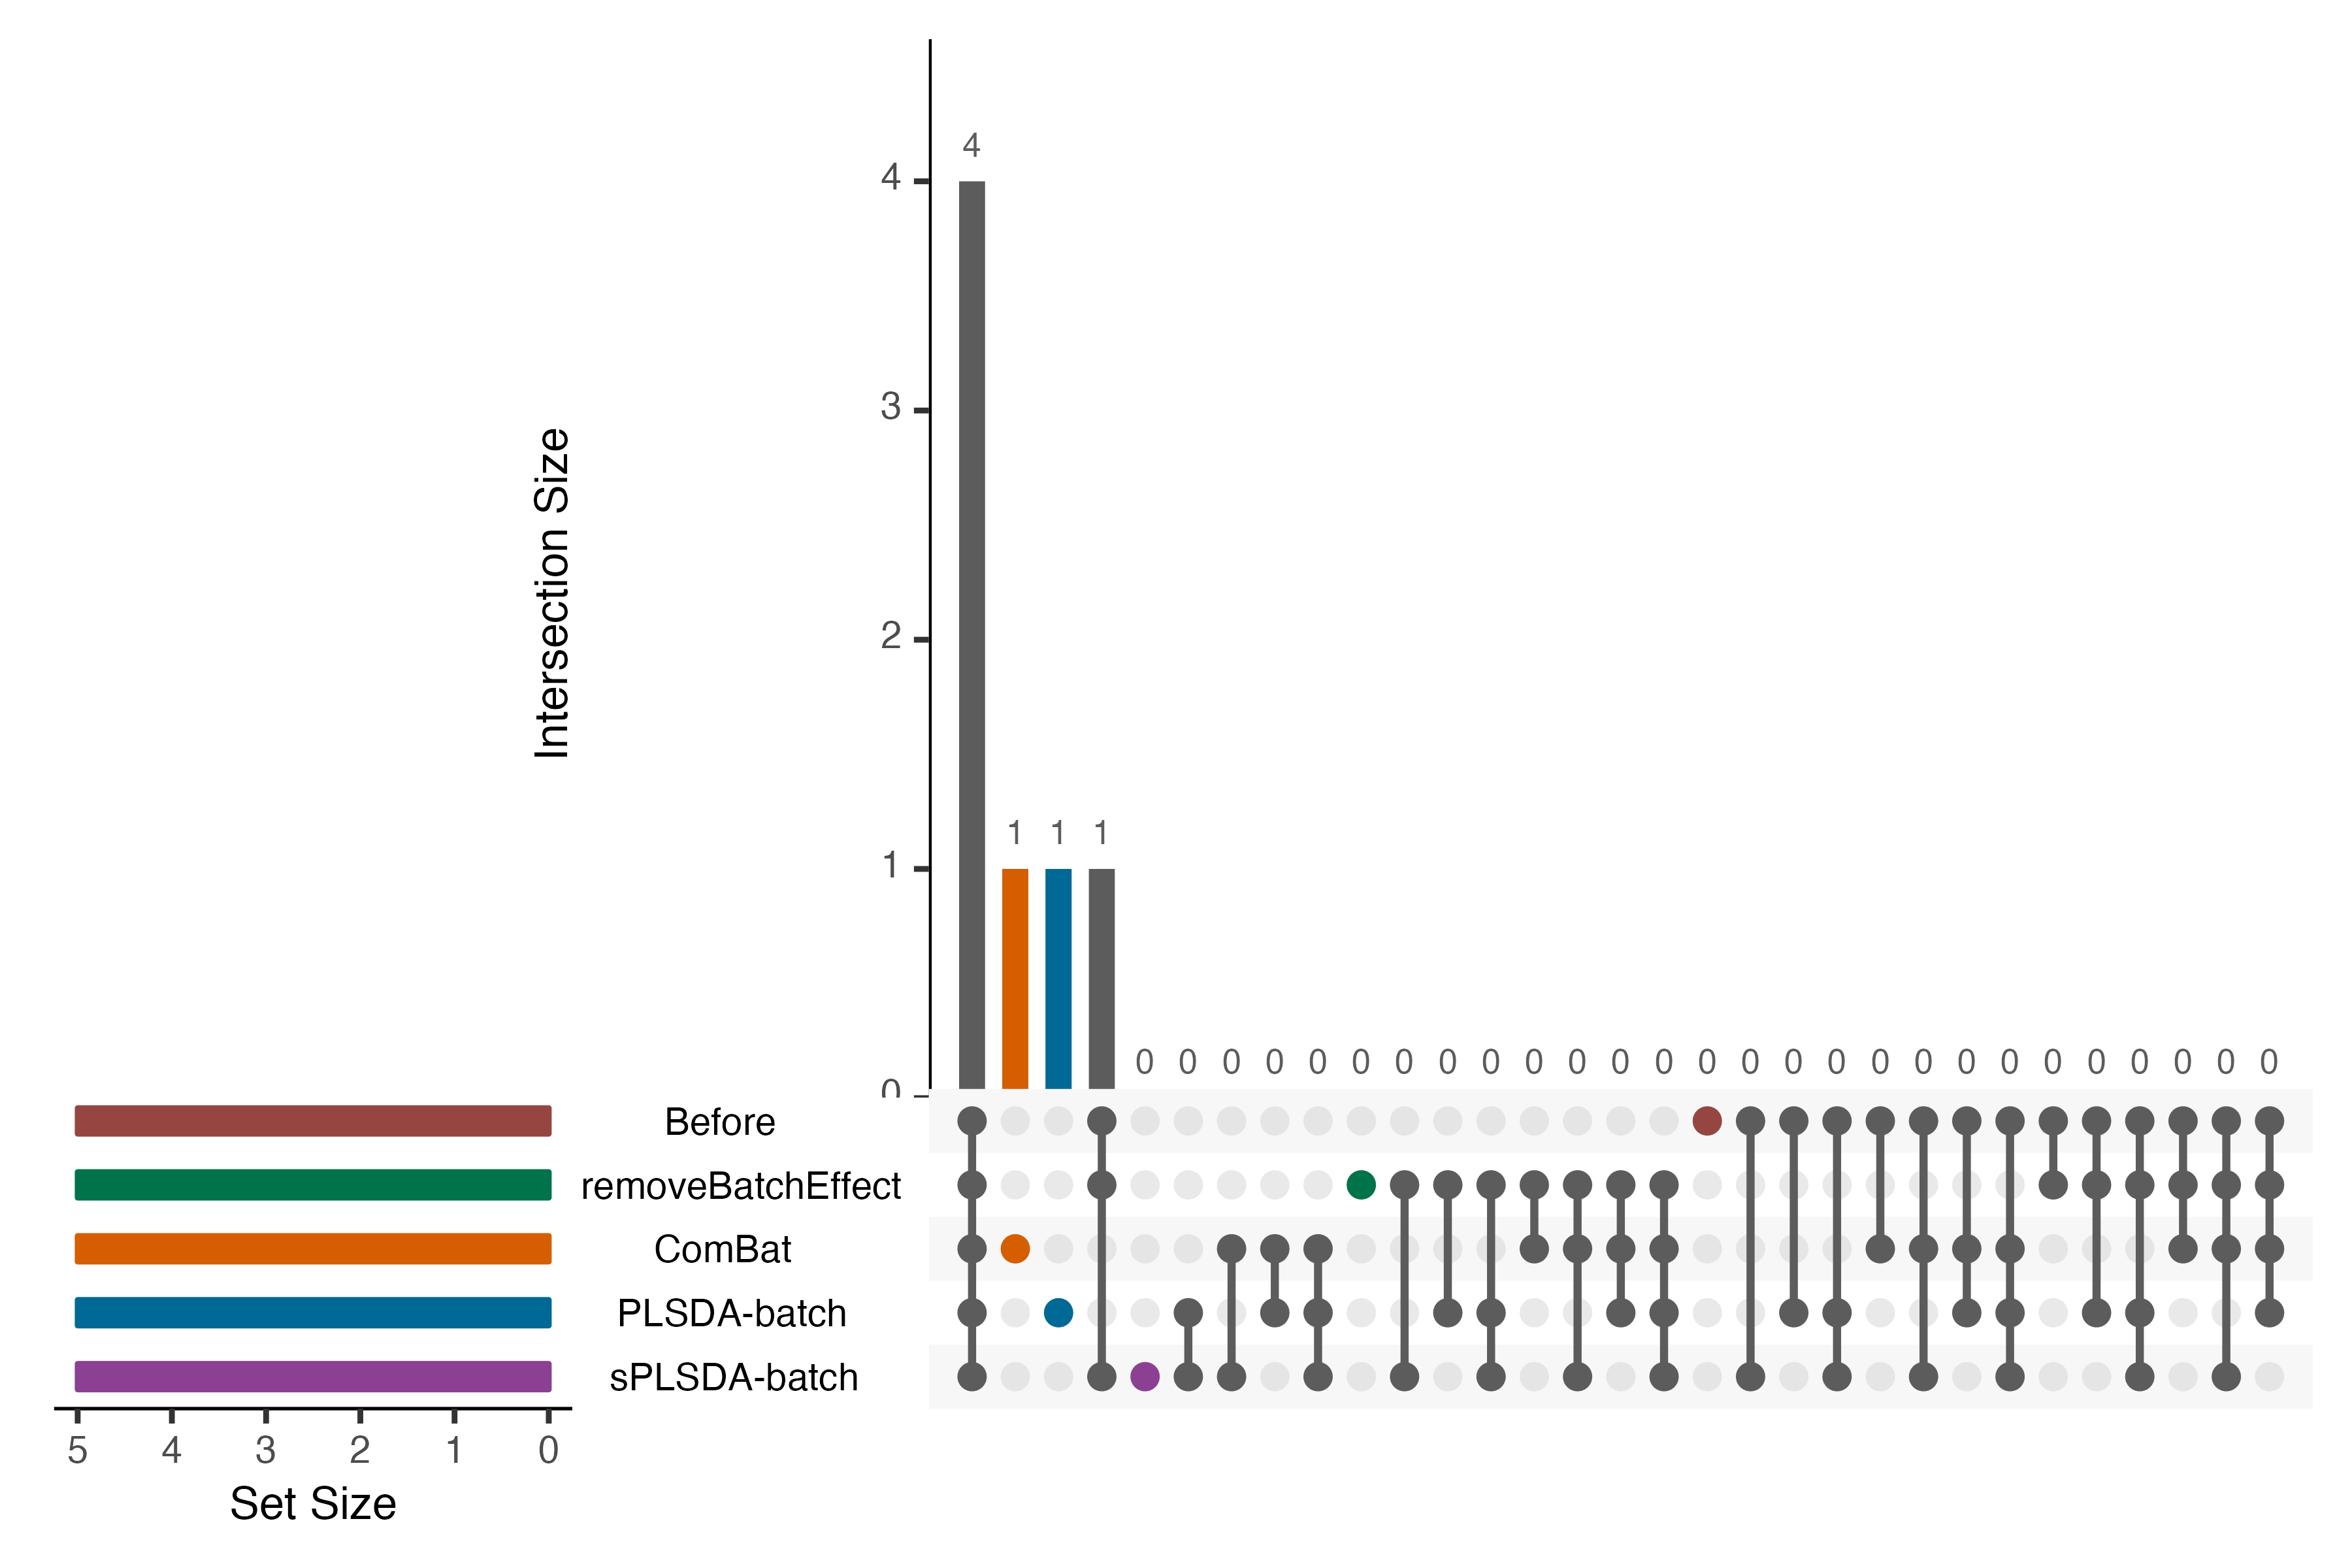
\includegraphics[width=1\linewidth]{PLSDAbatch_workflow_files/figure-latex/SpongeupsetR-1} 

}

\caption{UpSet plot showing overlap between variables selected from different corrected data for the sponge study.}\label{fig:SpongeupsetR}
\end{figure}

In the above figure, the left bars indicate the number of variables selected from each data corrected with different methods. The right bar plot combined with the scatterplot show different intersection and their aggregates. We obtained an overlap of 4 out of 5 selected variables between different corrected and uncorrected data. However, the data from each method still included unique variables that were not selected in the other corrected data, e.g., ComBat and PLSDA-batch. As \texttt{upset()} can only include five datasets at once, we only displayed the uncorrected data and four corrected data that had been more efficiently corrected for batch effects from our previous assessments compared to the other datasets.

\hypertarget{hfhs-data}{%
\section{HFHS data}\label{hfhs-data}}

\hypertarget{data-pre-processing-2}{%
\subsection{Data pre-processing}\label{data-pre-processing-2}}

\hypertarget{prefiltering}{%
\subsubsection{Prefiltering}\label{prefiltering}}

We load the \textcolor{olive}{HFHS data} stored internally with function \texttt{data()}.

\begin{Shaded}
\begin{Highlighting}[]
\FunctionTok{data}\NormalTok{(}\StringTok{\textquotesingle{}HFHS\_data\textquotesingle{}}\NormalTok{) }
\NormalTok{hfhs.count }\OtherTok{\textless{}{-}}\NormalTok{ HFHS\_data}\SpecialCharTok{$}\NormalTok{FullData}\SpecialCharTok{$}\NormalTok{X.count}
\FunctionTok{dim}\NormalTok{(hfhs.count)}
\end{Highlighting}
\end{Shaded}

\begin{verbatim}
## [1]  250 4524
\end{verbatim}

\begin{Shaded}
\begin{Highlighting}[]
\NormalTok{hfhs.filter.res }\OtherTok{\textless{}{-}} \FunctionTok{PreFL}\NormalTok{(}\AttributeTok{data =}\NormalTok{ hfhs.count)}
\NormalTok{hfhs.filter }\OtherTok{\textless{}{-}}\NormalTok{ hfhs.filter.res}\SpecialCharTok{$}\NormalTok{data.filter}
\FunctionTok{dim}\NormalTok{(hfhs.filter)}
\end{Highlighting}
\end{Shaded}

\begin{verbatim}
## [1] 250 515
\end{verbatim}

\begin{Shaded}
\begin{Highlighting}[]
\CommentTok{\# zero proportion before filtering}
\NormalTok{hfhs.filter.res}\SpecialCharTok{$}\NormalTok{zero.prob}
\end{Highlighting}
\end{Shaded}

\begin{verbatim}
## [1] 0.8490805
\end{verbatim}

\begin{Shaded}
\begin{Highlighting}[]
\CommentTok{\# zero proportion after filtering}
\FunctionTok{sum}\NormalTok{(hfhs.filter }\SpecialCharTok{==} \DecValTok{0}\NormalTok{)}\SpecialCharTok{/}\NormalTok{(}\FunctionTok{nrow}\NormalTok{(hfhs.filter) }\SpecialCharTok{*} \FunctionTok{ncol}\NormalTok{(hfhs.filter))}
\end{Highlighting}
\end{Shaded}

\begin{verbatim}
## [1] 0.2955184
\end{verbatim}

The raw \textcolor{olive}{HFHS data} include 4524 OTUs and 250 samples. We use the function \texttt{PreFL()} from our \textcolor{orange}{PLSDAbatch} R package to filter the data. After filtering, the \textcolor{olive}{HFHS data} were reduced to 515 OTUs and 250 samples. The proportion of zeroes was reduced from 85\% to 30\%.

\hypertarget{transformation-2}{%
\subsubsection{Transformation}\label{transformation-2}}

Prior to CLR transformation, we recommend adding 1 as the offset for the \textcolor{olive}{HFHS data} - that are raw count data. We use \texttt{logratio.transfo()} function in \textcolor{orange}{mixOmics} package to CLR transform the data.

\begin{Shaded}
\begin{Highlighting}[]
\NormalTok{hfhs.clr }\OtherTok{\textless{}{-}} \FunctionTok{logratio.transfo}\NormalTok{(}\AttributeTok{X =}\NormalTok{ hfhs.filter, }\AttributeTok{logratio =} \StringTok{\textquotesingle{}CLR\textquotesingle{}}\NormalTok{, }\AttributeTok{offset =} \DecValTok{1}\NormalTok{)}

\FunctionTok{class}\NormalTok{(hfhs.clr) }\OtherTok{\textless{}{-}} \StringTok{\textquotesingle{}matrix\textquotesingle{}}
\end{Highlighting}
\end{Shaded}

\hypertarget{batch-effect-detection-2}{%
\subsection{Batch effect detection}\label{batch-effect-detection-2}}

\hypertarget{pca-2}{%
\subsubsection{PCA}\label{pca-2}}

We apply \texttt{pca()} function from \textcolor{orange}{mixOmics} package to the \textcolor{olive}{HFHS data} and use \texttt{Scatter\_Density()} function from \textcolor{orange}{PLSDAbatch} to represent the PCA sample plot with densities.

\begin{Shaded}
\begin{Highlighting}[]
\NormalTok{hfhs.pca.before }\OtherTok{\textless{}{-}} \FunctionTok{pca}\NormalTok{(hfhs.clr, }\AttributeTok{ncomp =} \DecValTok{3}\NormalTok{, }\AttributeTok{scale =} \ConstantTok{TRUE}\NormalTok{)}

\NormalTok{hfhs.metadata }\OtherTok{\textless{}{-}}\NormalTok{ HFHS\_data}\SpecialCharTok{$}\NormalTok{FullData}\SpecialCharTok{$}\NormalTok{metadata}
\FunctionTok{rownames}\NormalTok{(hfhs.metadata) }\OtherTok{\textless{}{-}}\NormalTok{ hfhs.metadata}\SpecialCharTok{$}\NormalTok{SampleID}
\NormalTok{hfhs.metadata }\OtherTok{\textless{}{-}}\NormalTok{ hfhs.metadata[}\FunctionTok{rownames}\NormalTok{(hfhs.clr),]}

\NormalTok{hfhs.cage }\OtherTok{\textless{}{-}} \FunctionTok{as.factor}\NormalTok{(hfhs.metadata}\SpecialCharTok{$}\NormalTok{DietCage)}
\NormalTok{hfhs.day }\OtherTok{\textless{}{-}} \FunctionTok{as.factor}\NormalTok{(hfhs.metadata}\SpecialCharTok{$}\NormalTok{Day)}
\NormalTok{hfhs.trt }\OtherTok{\textless{}{-}} \FunctionTok{as.factor}\NormalTok{(hfhs.metadata}\SpecialCharTok{$}\NormalTok{Diet)}
\FunctionTok{names}\NormalTok{(hfhs.cage) }\OtherTok{=} \FunctionTok{names}\NormalTok{(hfhs.day) }\OtherTok{=} \FunctionTok{names}\NormalTok{(hfhs.trt) }\OtherTok{=}\NormalTok{ hfhs.metadata}\SpecialCharTok{$}\NormalTok{SampleID}

\NormalTok{hfhs.pca.before.cage.plot }\OtherTok{\textless{}{-}} 
  \FunctionTok{Scatter\_Density}\NormalTok{(}\AttributeTok{object =}\NormalTok{ hfhs.pca.before, }
                  \AttributeTok{batch =}\NormalTok{ hfhs.cage, }
                  \AttributeTok{trt =}\NormalTok{ hfhs.trt, }
                  \AttributeTok{title =} \StringTok{\textquotesingle{}HFHS data\textquotesingle{}}\NormalTok{, }
                  \AttributeTok{trt.legend.title =} \StringTok{\textquotesingle{}Diet\textquotesingle{}}\NormalTok{,}
                  \AttributeTok{batch.legend.title =} \StringTok{\textquotesingle{}Cage\textquotesingle{}}\NormalTok{)}
\end{Highlighting}
\end{Shaded}

\begin{figure}

{\centering 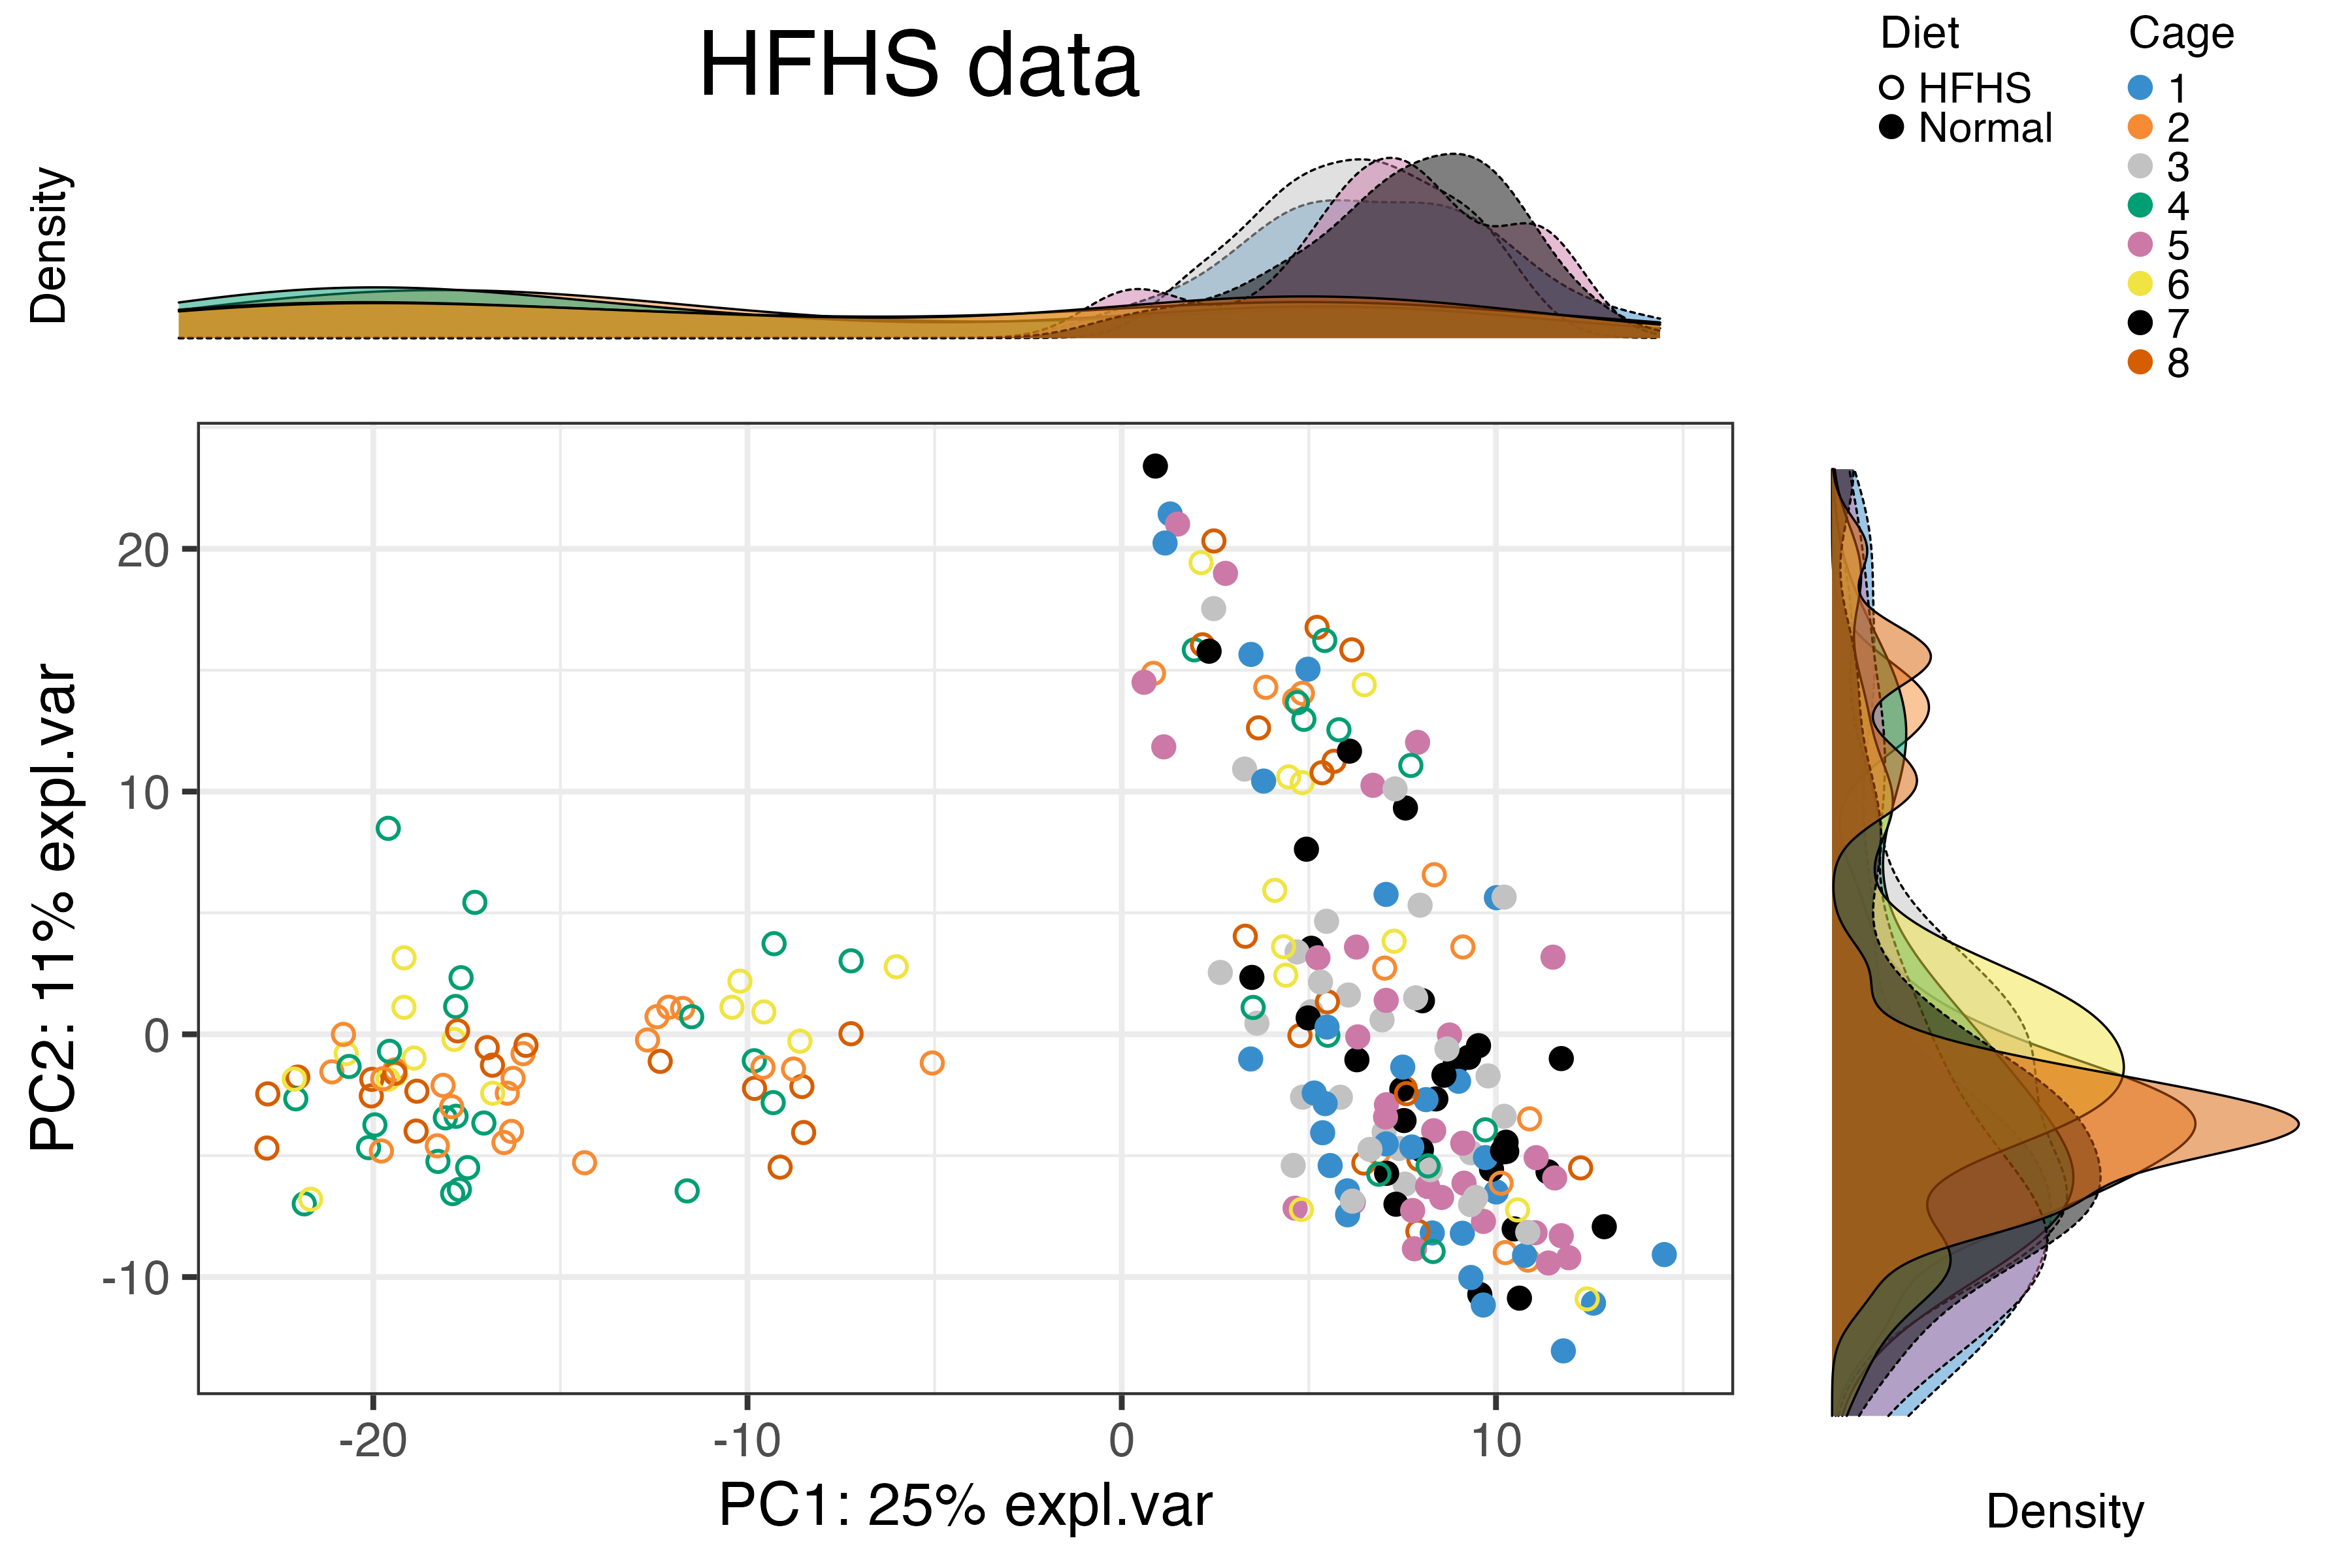
\includegraphics[width=0.6\linewidth]{PLSDAbatch_workflow_files/figure-latex/HFHSpcaBefore1-1} 

}

\caption{The PCA sample plot with densities coloured by cages in the HFHS data.}\label{fig:HFHSpcaBefore1}
\end{figure}

In the above figure, part of the samples with different diets were mixed together, while all the samples from different batches (i.e., cages) were well mixed and not distinct. This result indicates no cage effect for the whole data and no treatment effect for part of samples.

\begin{Shaded}
\begin{Highlighting}[]
\NormalTok{hfhs.pca.before.day.plot }\OtherTok{\textless{}{-}} 
  \FunctionTok{Scatter\_Density}\NormalTok{(}\AttributeTok{object =}\NormalTok{ hfhs.pca.before, }
                  \AttributeTok{batch =}\NormalTok{ hfhs.day, }
                  \AttributeTok{trt =}\NormalTok{ hfhs.trt, }
                  \AttributeTok{title =} \StringTok{\textquotesingle{}HFHS data\textquotesingle{}}\NormalTok{, }
                  \AttributeTok{trt.legend.title =} \StringTok{\textquotesingle{}Diet\textquotesingle{}}\NormalTok{,}
                  \AttributeTok{batch.legend.title =} \StringTok{\textquotesingle{}Day\textquotesingle{}}\NormalTok{)}
\end{Highlighting}
\end{Shaded}

\begin{figure}

{\centering 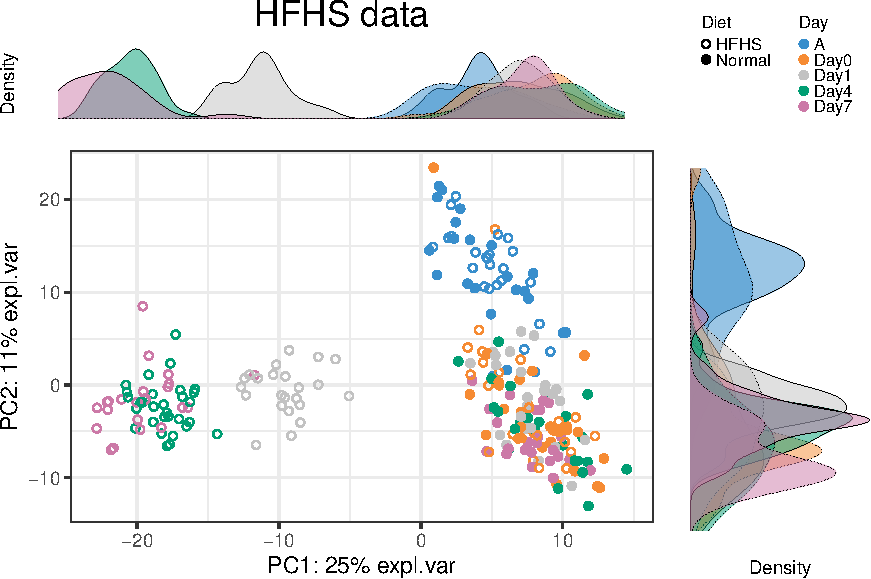
\includegraphics[width=0.6\linewidth]{PLSDAbatch_workflow_files/figure-latex/HFHSpcaBefore2-1} 

}

\caption{Figure 11: The PCA sample plot with densities coloured by days in the HFHS data.}\label{fig:HFHSpcaBefore2}
\end{figure}

As shown in the above figure, we did not observe a difference between samples with different diets on arrival day ``A'' and ``Day0''. This result was consistent with the experimental design, as mice were not treated with different diets on these two days. We thus removed the samples from these two days.

\begin{Shaded}
\begin{Highlighting}[]
\CommentTok{\# remove samples from arrival day and day0}
\NormalTok{hfhs.dA0.idx }\OtherTok{\textless{}{-}} \FunctionTok{c}\NormalTok{(}\FunctionTok{which}\NormalTok{(hfhs.day }\SpecialCharTok{==} \StringTok{\textquotesingle{}A\textquotesingle{}}\NormalTok{), }\FunctionTok{which}\NormalTok{(hfhs.day }\SpecialCharTok{==} \StringTok{\textquotesingle{}Day0\textquotesingle{}}\NormalTok{))}
\NormalTok{hfhs.clr.less }\OtherTok{\textless{}{-}}\NormalTok{ hfhs.clr[}\SpecialCharTok{{-}}\NormalTok{hfhs.dA0.idx,]}
\NormalTok{hfhs.metadata.less }\OtherTok{\textless{}{-}}\NormalTok{ hfhs.metadata[}\SpecialCharTok{{-}}\NormalTok{hfhs.dA0.idx,]}

\NormalTok{hfhs.cage.less }\OtherTok{\textless{}{-}} \FunctionTok{as.factor}\NormalTok{(hfhs.metadata.less}\SpecialCharTok{$}\NormalTok{DietCage)}
\NormalTok{hfhs.day.less }\OtherTok{\textless{}{-}} \FunctionTok{as.factor}\NormalTok{(hfhs.metadata.less}\SpecialCharTok{$}\NormalTok{Day)}
\NormalTok{hfhs.trt.less }\OtherTok{\textless{}{-}} \FunctionTok{as.factor}\NormalTok{(hfhs.metadata.less}\SpecialCharTok{$}\NormalTok{Diet)}
\FunctionTok{names}\NormalTok{(hfhs.cage.less) }\OtherTok{=} \FunctionTok{names}\NormalTok{(hfhs.day.less) }\OtherTok{=} 
  \FunctionTok{names}\NormalTok{(hfhs.trt.less) }\OtherTok{=}\NormalTok{ hfhs.metadata.less}\SpecialCharTok{$}\NormalTok{SampleID}

\NormalTok{hfhs.less.pca.before }\OtherTok{\textless{}{-}} \FunctionTok{pca}\NormalTok{(hfhs.clr.less, }\AttributeTok{ncomp =} \DecValTok{3}\NormalTok{, }\AttributeTok{scale =} \ConstantTok{TRUE}\NormalTok{)}

\NormalTok{hfhs.less.pca.before.cage.plot }\OtherTok{\textless{}{-}} 
  \FunctionTok{Scatter\_Density}\NormalTok{(}\AttributeTok{object =}\NormalTok{ hfhs.less.pca.before, }
                  \AttributeTok{batch =}\NormalTok{ hfhs.cage.less, }
                  \AttributeTok{trt =}\NormalTok{ hfhs.trt.less, }
                  \AttributeTok{title =} \StringTok{\textquotesingle{}HFHS data\textquotesingle{}}\NormalTok{, }
                  \AttributeTok{trt.legend.title =} \StringTok{\textquotesingle{}Diet\textquotesingle{}}\NormalTok{,}
                  \AttributeTok{batch.legend.title =} \StringTok{\textquotesingle{}Cage\textquotesingle{}}\NormalTok{)}
\end{Highlighting}
\end{Shaded}

\begin{figure}

{\centering 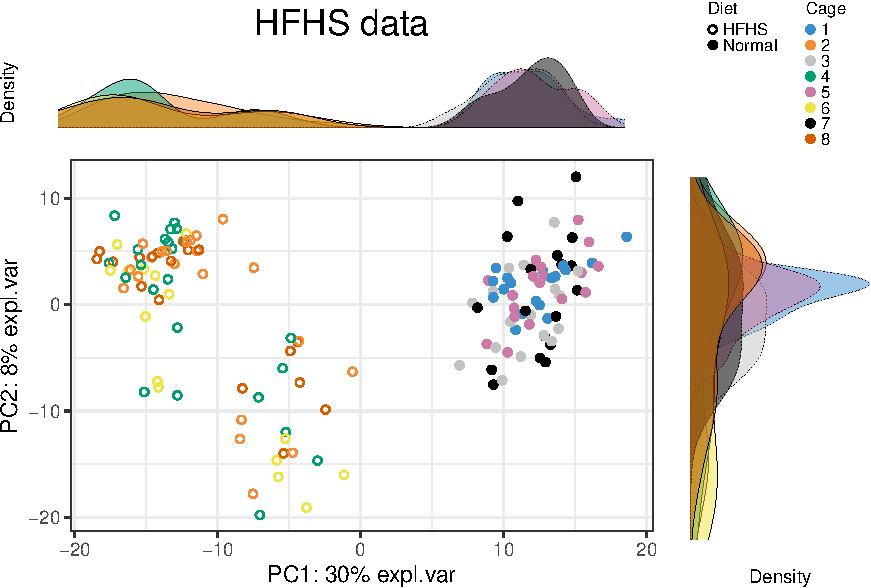
\includegraphics[width=0.6\linewidth]{PLSDAbatch_workflow_files/figure-latex/HFHSpcaBeforeNew1-1} 

}

\caption{The PCA sample plot with densities coloured by cages in the reduced HFHS data.}\label{fig:HFHSpcaBeforeNew1}
\end{figure}

\begin{Shaded}
\begin{Highlighting}[]
\NormalTok{hfhs.less.pca.before.day.plot }\OtherTok{\textless{}{-}} 
  \FunctionTok{Scatter\_Density}\NormalTok{(}\AttributeTok{object =}\NormalTok{ hfhs.less.pca.before, }
                  \AttributeTok{batch =}\NormalTok{ hfhs.day.less, }
                  \AttributeTok{trt =}\NormalTok{ hfhs.trt.less, }
                  \AttributeTok{title =} \StringTok{\textquotesingle{}HFHS data\textquotesingle{}}\NormalTok{, }
                  \AttributeTok{trt.legend.title =} \StringTok{\textquotesingle{}Diet\textquotesingle{}}\NormalTok{,}
                  \AttributeTok{batch.legend.title =} \StringTok{\textquotesingle{}Day\textquotesingle{}}\NormalTok{)}
\end{Highlighting}
\end{Shaded}

\begin{figure}

{\centering 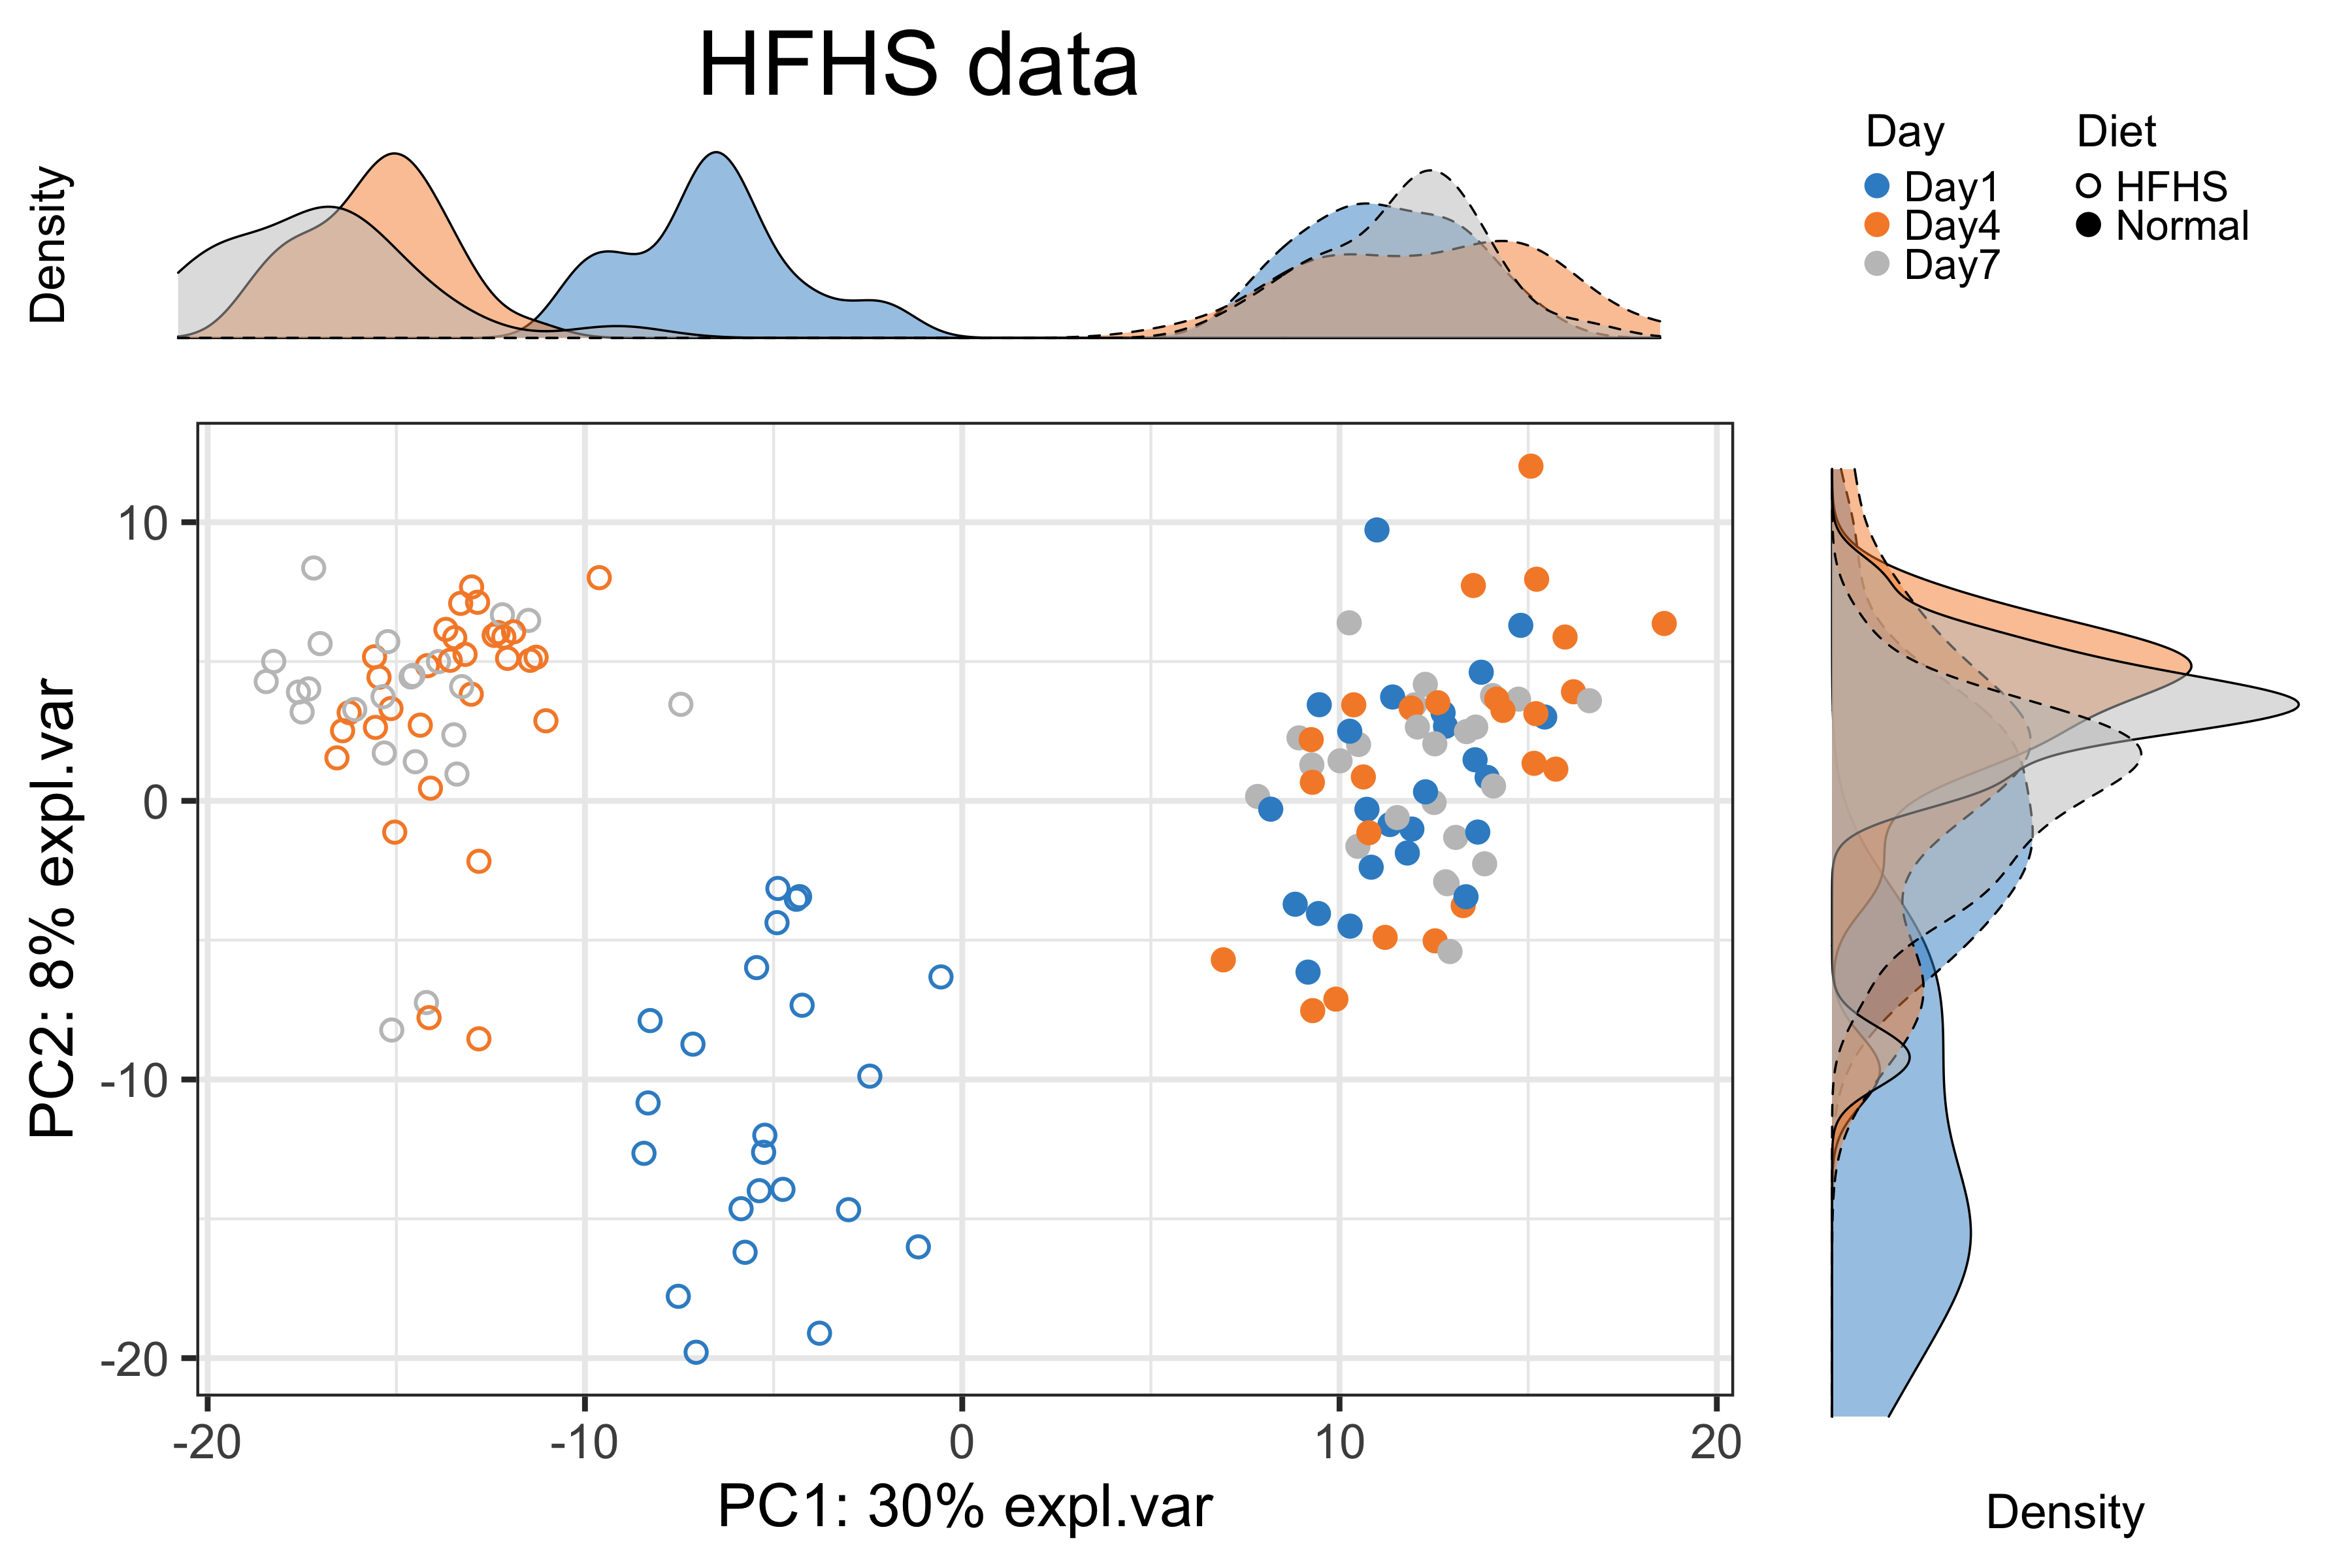
\includegraphics[width=0.6\linewidth]{PLSDAbatch_workflow_files/figure-latex/HFHSpcaBeforeNew2-1} 

}

\caption{The PCA sample plot with densities coloured by days in the reduced HFHS data.}\label{fig:HFHSpcaBeforeNew2}
\end{figure}

We observed a substantial diet variation on component 1, no cage variation, and a difference between samples collected on ``Day1'' and the other days with the HFHS diet as shown in the above figures.

\hypertarget{heatmap-2}{%
\subsubsection{Heatmap}\label{heatmap-2}}

We produce a heatmap using \textcolor{orange}{pheatmap} package. The data first need to be scaled on both OTUs and samples.

\begin{Shaded}
\begin{Highlighting}[]
\CommentTok{\# scale the clr data on both OTUs and samples}
\NormalTok{hfhs.clr.s }\OtherTok{\textless{}{-}} \FunctionTok{scale}\NormalTok{(hfhs.clr.less, }\AttributeTok{center =}\NormalTok{ T, }\AttributeTok{scale =}\NormalTok{ T)}
\NormalTok{hfhs.clr.ss }\OtherTok{\textless{}{-}} \FunctionTok{scale}\NormalTok{(}\FunctionTok{t}\NormalTok{(hfhs.clr.s), }\AttributeTok{center =}\NormalTok{ T, }\AttributeTok{scale =}\NormalTok{ T)}

\CommentTok{\# The cage effect}
\NormalTok{hfhs.anno\_col }\OtherTok{\textless{}{-}} \FunctionTok{data.frame}\NormalTok{(}\AttributeTok{Cage =}\NormalTok{ hfhs.cage.less, }
                            \AttributeTok{Day =}\NormalTok{ hfhs.day.less, }
                            \AttributeTok{Treatment =}\NormalTok{ hfhs.trt.less)}
\NormalTok{hfhs.anno\_colors }\OtherTok{\textless{}{-}} \FunctionTok{list}\NormalTok{(}\AttributeTok{Cage =} \FunctionTok{color.mixo}\NormalTok{(}\DecValTok{1}\SpecialCharTok{:}\DecValTok{8}\NormalTok{), }
                         \AttributeTok{Day =} \FunctionTok{color.mixo}\NormalTok{(}\DecValTok{1}\SpecialCharTok{:}\DecValTok{3}\NormalTok{),}
                         \AttributeTok{Treatment =} \FunctionTok{pb\_color}\NormalTok{(}\DecValTok{1}\SpecialCharTok{:}\DecValTok{2}\NormalTok{))}
\FunctionTok{names}\NormalTok{(hfhs.anno\_colors}\SpecialCharTok{$}\NormalTok{Cage) }\OtherTok{=} \FunctionTok{levels}\NormalTok{(hfhs.cage.less)}
\FunctionTok{names}\NormalTok{(hfhs.anno\_colors}\SpecialCharTok{$}\NormalTok{Day) }\OtherTok{=} \FunctionTok{levels}\NormalTok{(hfhs.day.less)}
\FunctionTok{names}\NormalTok{(hfhs.anno\_colors}\SpecialCharTok{$}\NormalTok{Treatment) }\OtherTok{=} \FunctionTok{levels}\NormalTok{(hfhs.trt.less)}

\FunctionTok{pheatmap}\NormalTok{(hfhs.clr.ss, }
         \AttributeTok{cluster\_rows =}\NormalTok{ F, }
         \AttributeTok{fontsize\_row =} \DecValTok{4}\NormalTok{, }
         \AttributeTok{fontsize\_col =} \DecValTok{6}\NormalTok{,}
         \AttributeTok{fontsize =} \DecValTok{8}\NormalTok{,}
         \AttributeTok{clustering\_distance\_rows =} \StringTok{\textquotesingle{}euclidean\textquotesingle{}}\NormalTok{,}
         \AttributeTok{clustering\_method =} \StringTok{\textquotesingle{}ward.D\textquotesingle{}}\NormalTok{,}
         \AttributeTok{treeheight\_row =} \DecValTok{30}\NormalTok{,}
         \AttributeTok{annotation\_col =}\NormalTok{ hfhs.anno\_col,}
         \AttributeTok{annotation\_colors =}\NormalTok{ hfhs.anno\_colors,}
         \AttributeTok{border\_color =} \StringTok{\textquotesingle{}NA\textquotesingle{}}\NormalTok{,}
         \AttributeTok{main =} \StringTok{\textquotesingle{}HFHS data {-} Scaled\textquotesingle{}}\NormalTok{)}
\end{Highlighting}
\end{Shaded}

\begin{figure}

{\centering 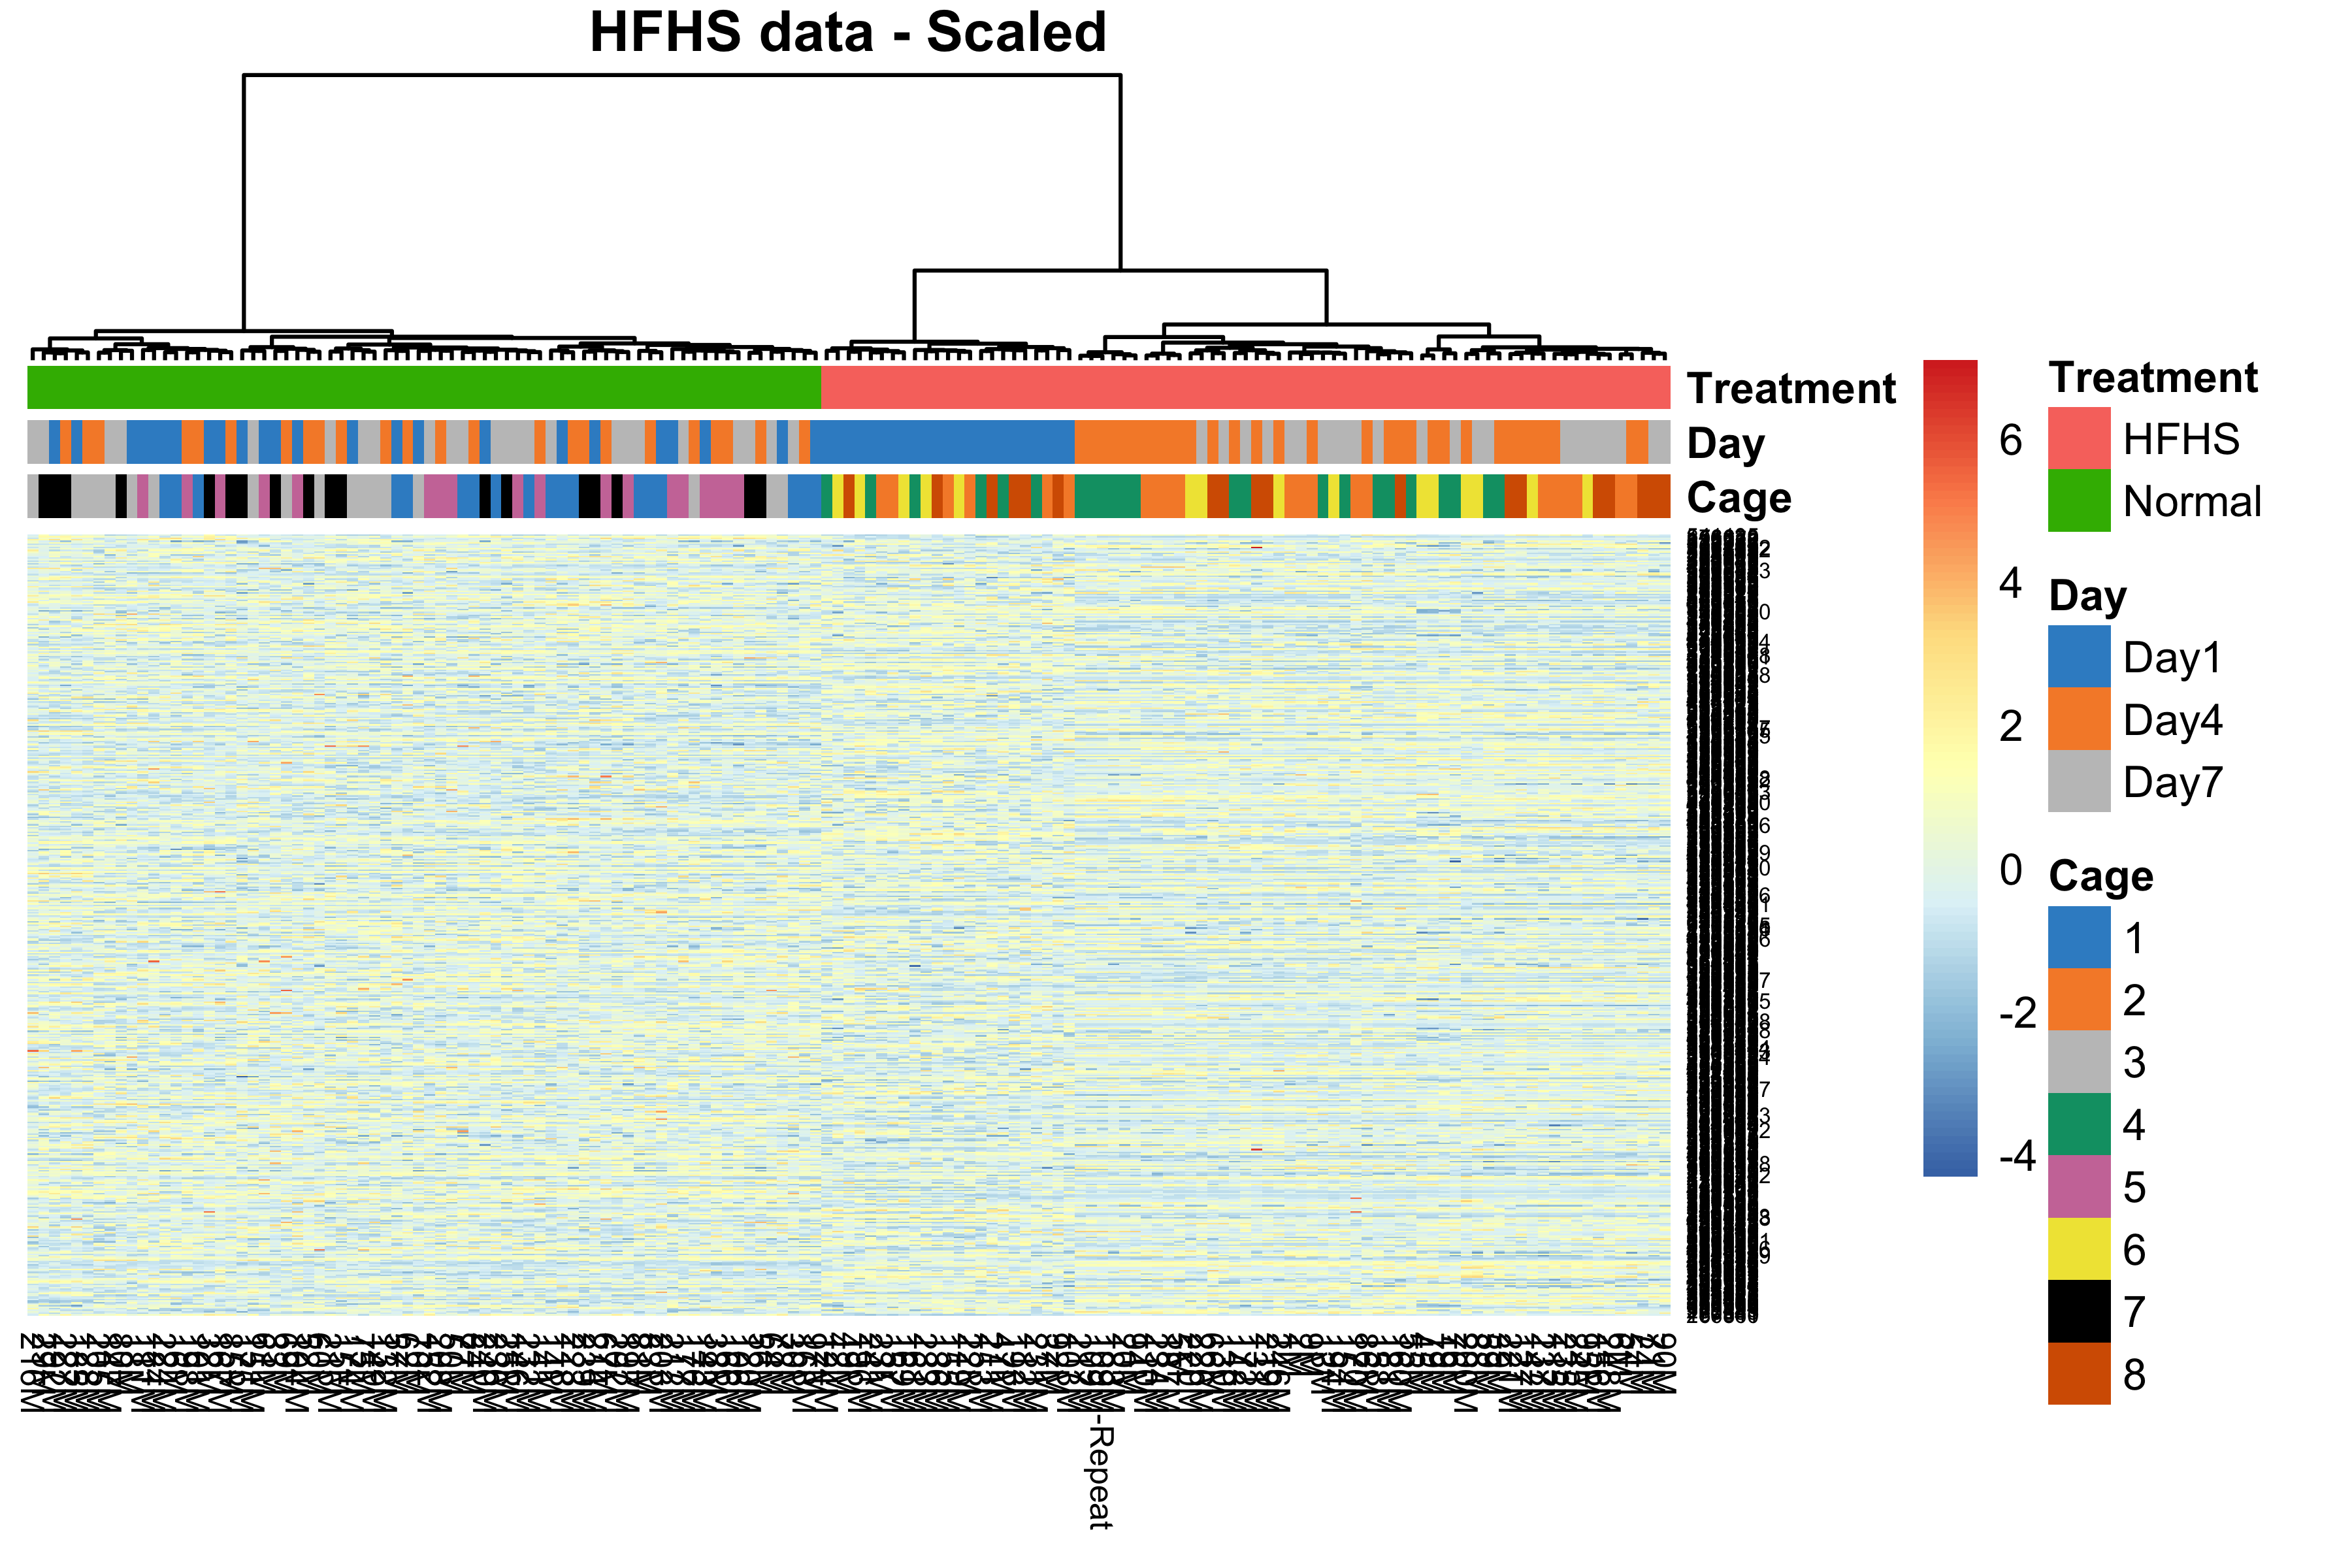
\includegraphics[width=0.9\linewidth]{PLSDAbatch_workflow_files/figure-latex/HFHSheatmapS-1} 

}

\caption{Hierarchical clustering for samples in the HFHS data.}\label{fig:HFHSheatmapS}
\end{figure}

In the above figure, samples in the \textcolor{olive}{HFHS data} were clustered according to the treatments not cages, indicating no cage effect and a strong treatment effect. Samples from the batch ``Day1'' were clustered and distinct from the other batches with diet HFHS but not the normal diet, indicating a day effect but very weak.

\hypertarget{prda-2}{%
\subsubsection{pRDA}\label{prda-2}}

We apply pRDA with \texttt{varpart()} function from \textcolor{orange}{vegan} R package.

\begin{Shaded}
\begin{Highlighting}[]
\NormalTok{hfhs.factors.df }\OtherTok{\textless{}{-}} \FunctionTok{data.frame}\NormalTok{(}\AttributeTok{trt =}\NormalTok{ hfhs.trt.less, }
                              \AttributeTok{cage =}\NormalTok{ hfhs.cage.less, }
                              \AttributeTok{day =}\NormalTok{ hfhs.day.less)}
\NormalTok{hfhs.rda.cage.before }\OtherTok{\textless{}{-}} \FunctionTok{varpart}\NormalTok{(hfhs.clr.less, }\SpecialCharTok{\textasciitilde{}}\NormalTok{ trt, }\SpecialCharTok{\textasciitilde{}}\NormalTok{ cage, }
                                \AttributeTok{data =}\NormalTok{ hfhs.factors.df, }\AttributeTok{scale =}\NormalTok{ T)}
\NormalTok{hfhs.rda.cage.before}\SpecialCharTok{$}\NormalTok{part}\SpecialCharTok{$}\NormalTok{indfract}
\end{Highlighting}
\end{Shaded}

\begin{verbatim}
##                 Df R.squared Adj.R.squared Testable
## [a] = X1|X2      0        NA  7.771561e-16    FALSE
## [b] = X2|X1      6        NA  1.277627e-02     TRUE
## [c]              0        NA  2.713111e-01    FALSE
## [d] = Residuals NA        NA  7.159126e-01    FALSE
\end{verbatim}

In the result, \texttt{X1} and \texttt{X2} represent the first and second covariates fitted in the model. \texttt{{[}a{]}}, \texttt{{[}b{]}} represent the independent proportion of variance explained by \texttt{X1} and \texttt{X2} respectively, and \texttt{{[}c{]}} represents the intersection variance shared between \texttt{X1} and \texttt{X2}. In the \textcolor{olive}{HFHS data}, the cage and diet effects have a nested batch x treatment design that is extremely unbalanced. We didn't detect any treatment variance (indicated in line \texttt{{[}a{]}}, Adj.R.squared = 0) but considerable intersection variance (indicated in line \texttt{{[}c{]}}, Adj.R.squared = 0.271). Thus, all the treatment variance was explained by the intersection variance shared with batch variance. It means batch and treatment effects are collinear. Therefore, the cage effect in the \textcolor{olive}{HFHS data} can only be accounted for with a linear mixed model, as detailed in section \textbf{accounting for batch effects} method ``Linear regression''.

\begin{Shaded}
\begin{Highlighting}[]
\NormalTok{hfhs.rda.day.before }\OtherTok{\textless{}{-}} \FunctionTok{varpart}\NormalTok{(hfhs.clr.less, }\SpecialCharTok{\textasciitilde{}}\NormalTok{ trt, }\SpecialCharTok{\textasciitilde{}}\NormalTok{ day, }
                               \AttributeTok{data =}\NormalTok{ hfhs.factors.df, }\AttributeTok{scale =}\NormalTok{ T)}
\NormalTok{hfhs.rda.day.before}\SpecialCharTok{$}\NormalTok{part}\SpecialCharTok{$}\NormalTok{indfract}
\end{Highlighting}
\end{Shaded}

\begin{verbatim}
##                 Df R.squared Adj.R.squared Testable
## [a] = X1|X2      1        NA  0.2721810304     TRUE
## [b] = X2|X1      2        NA  0.0361767632     TRUE
## [c]              0        NA -0.0008699296    FALSE
## [d] = Residuals NA        NA  0.6925121361    FALSE
\end{verbatim}

For the day and diet effects, the batch x treatment design is balanced. There was no intersection variance (indicated in line \texttt{{[}c{]}}, Adj.R.squared = 0). The proportion of treatment variance was much higher than batch variance as indicated in lines \texttt{{[}a{]}} (Adj.R.squared = 0.272) and \texttt{{[}b{]}} (Adj.R.squared = 0.036).

\hypertarget{managing-batch-effects-2}{%
\subsection{Managing batch effects}\label{managing-batch-effects-2}}

\hypertarget{accounting-for-batch-effects-1}{%
\subsubsection{Accounting for batch effects}\label{accounting-for-batch-effects-1}}

The methods that we use to account for batch effects include the methods designed for microbiome data: zero-inflated Gaussian (ZIG) mixture model and the methods adapted for microbiome data: linear regression, SVA and RUV4. Among them, SVA and RUV4 are designed for unknown batch effects.

\textbf{Methods designed for microbiome data}

\textbf{Zero-inflated Gaussian mixture model} To use the ZIG model, we first create a \texttt{MRexperiment} object applying \texttt{newMRexperiment()} (from \textcolor{orange}{metagenomeSeq} package) to microbiome counts and annotated data frames with metadata and taxonomic information generated with \texttt{AnnotatedDataFrame()} from \textcolor{orange}{Biobase} package.

\begin{Shaded}
\begin{Highlighting}[]
\CommentTok{\# Creating a MRexperiment object (make sure no NA in metadata)}
\FunctionTok{rownames}\NormalTok{(HFHS\_data}\SpecialCharTok{$}\NormalTok{FullData}\SpecialCharTok{$}\NormalTok{metadata) }\OtherTok{\textless{}{-}} \FunctionTok{rownames}\NormalTok{(HFHS\_data}\SpecialCharTok{$}\NormalTok{FullData}\SpecialCharTok{$}\NormalTok{X.count)}
\NormalTok{HFHS.phenotypeData }\OtherTok{=} 
  \FunctionTok{AnnotatedDataFrame}\NormalTok{(}\AttributeTok{data =}\NormalTok{ HFHS\_data}\SpecialCharTok{$}\NormalTok{FullData}\SpecialCharTok{$}\NormalTok{metadata[}\SpecialCharTok{{-}}\NormalTok{hfhs.dA0.idx,])}
\NormalTok{HFHS.taxaData }\OtherTok{=} 
  \FunctionTok{AnnotatedDataFrame}\NormalTok{(}\AttributeTok{data =} \FunctionTok{as.data.frame}\NormalTok{(HFHS\_data}\SpecialCharTok{$}\NormalTok{FullData}\SpecialCharTok{$}\NormalTok{taxa))}
\NormalTok{HFHS.obj }\OtherTok{=} \FunctionTok{newMRexperiment}\NormalTok{(}\AttributeTok{counts =} 
                             \FunctionTok{t}\NormalTok{(HFHS\_data}\SpecialCharTok{$}\NormalTok{FullData}\SpecialCharTok{$}\NormalTok{X.count[}\SpecialCharTok{{-}}\NormalTok{hfhs.dA0.idx,]),}
                           \AttributeTok{phenoData =}\NormalTok{ HFHS.phenotypeData, }
                           \AttributeTok{featureData =}\NormalTok{ HFHS.taxaData)}
\NormalTok{HFHS.obj}
\end{Highlighting}
\end{Shaded}

\begin{verbatim}
## MRexperiment (storageMode: environment)
## assayData: 4524 features, 149 samples 
##   element names: counts 
## protocolData: none
## phenoData
##   sampleNames: 109M 131M ... 39M (149 total)
##   varLabels: SampleID MouseID ... Replicated (14 total)
##   varMetadata: labelDescription
## featureData
##   featureNames: 4333897 541135 ... 228232 (4524 total)
##   fvarLabels: Kingdom Phylum ... Species (7 total)
##   fvarMetadata: labelDescription
## experimentData: use 'experimentData(object)'
## Annotation:
\end{verbatim}

The \textcolor{olive}{HFHS data} are then filtered with \texttt{filterData()} function (from \textcolor{orange}{metagenomeSeq}). We can use \texttt{MRcounts()} to extract the count data from the \texttt{MRexperiment} object.

\begin{Shaded}
\begin{Highlighting}[]
\CommentTok{\# filtering data to maintain a threshold of minimum depth or OTU presence}
\FunctionTok{dim}\NormalTok{(}\FunctionTok{MRcounts}\NormalTok{(HFHS.obj))}
\end{Highlighting}
\end{Shaded}

\begin{verbatim}
## [1] 4524  149
\end{verbatim}

\begin{Shaded}
\begin{Highlighting}[]
\NormalTok{HFHS.obj }\OtherTok{=} \FunctionTok{filterData}\NormalTok{(}\AttributeTok{obj =}\NormalTok{ HFHS.obj, }\AttributeTok{present =} \DecValTok{20}\NormalTok{, }\AttributeTok{depth =} \DecValTok{5}\NormalTok{)}
\FunctionTok{dim}\NormalTok{(}\FunctionTok{MRcounts}\NormalTok{(HFHS.obj))}
\end{Highlighting}
\end{Shaded}

\begin{verbatim}
## [1] 1255  149
\end{verbatim}

After filtering, the \textcolor{olive}{HFHS data} were reduced to 1255 OTUs and 149 samples.

We calculate the percentile for CSS normalisation with \texttt{cumNormStatFast()} function (from \textcolor{orange}{metagenomeSeq} package). The CSS normalisation is applied with \texttt{cumNorm()} and the normalised data can be exported using \texttt{MRcounts()} with \texttt{norm\ =\ TRUE}. The normalisation scaling factors for each sample, which are the sum of counts up to the calculated percentile, can be accessed through \texttt{normFactors()}. We calculate the log transformed scaling factors by diving them with their median, which are better than the default scaling factors that are divided by 1000 (\texttt{log2(normFactors(obj)/1000\ +\ 1)}).

\begin{Shaded}
\begin{Highlighting}[]
\CommentTok{\# calculate the percentile for CSS normalisation}
\NormalTok{HFHS.pctl }\OtherTok{=} \FunctionTok{cumNormStatFast}\NormalTok{(}\AttributeTok{obj =}\NormalTok{ HFHS.obj)}
\CommentTok{\# CSS normalisation}
\NormalTok{HFHS.obj }\OtherTok{\textless{}{-}} \FunctionTok{cumNorm}\NormalTok{(}\AttributeTok{obj =}\NormalTok{ HFHS.obj, }\AttributeTok{p =}\NormalTok{ HFHS.pctl)}
\CommentTok{\# export normalised data}
\NormalTok{HFHS.norm.data }\OtherTok{\textless{}{-}} \FunctionTok{MRcounts}\NormalTok{(}\AttributeTok{obj =}\NormalTok{ HFHS.obj, }\AttributeTok{norm =} \ConstantTok{TRUE}\NormalTok{)}

\CommentTok{\# normalisation scaling factors for each sample }
\NormalTok{HFHS.normFactor }\OtherTok{=} \FunctionTok{normFactors}\NormalTok{(}\AttributeTok{object =}\NormalTok{ HFHS.obj)}
\NormalTok{HFHS.normFactor }\OtherTok{=} \FunctionTok{log2}\NormalTok{(HFHS.normFactor}\SpecialCharTok{/}\FunctionTok{median}\NormalTok{(HFHS.normFactor) }\SpecialCharTok{+} \DecValTok{1}\NormalTok{)}
\end{Highlighting}
\end{Shaded}

As the ZIG model applies a linear model, the cage effect cannot be fitted. Moreover, the cage effect is very weak which only accounted for 1.3\% of the total data variance calculated with pRDA. Thus we only fit and account for the day effect. We create a design matrix with treatment variable (\texttt{Diet\_effect}), batch variable (\texttt{Day\_effect}) and the log transformed scaling factors by using \texttt{model.matrix()}, and then apply the ZIG model by \texttt{fitZig()} function. We set \texttt{useCSSoffset\ =\ FALSE} to avoid using the default scaling factors as we have already included our customised scaling factor (\texttt{HFHS.normFactor}) in the design matrix.

\begin{Shaded}
\begin{Highlighting}[]
\CommentTok{\# treatment variable}
\NormalTok{Diet\_effect }\OtherTok{=} \FunctionTok{pData}\NormalTok{(}\AttributeTok{object =}\NormalTok{ HFHS.obj)}\SpecialCharTok{$}\NormalTok{Diet}

\CommentTok{\# batch variable}
\NormalTok{Day\_effect }\OtherTok{=} \FunctionTok{pData}\NormalTok{(}\AttributeTok{object =}\NormalTok{ HFHS.obj)}\SpecialCharTok{$}\NormalTok{Day}

\CommentTok{\# build a design matrix}
\NormalTok{HFHS.mod.full }\OtherTok{=} \FunctionTok{model.matrix}\NormalTok{(}\SpecialCharTok{\textasciitilde{}}\NormalTok{ Diet\_effect }\SpecialCharTok{+}\NormalTok{ Day\_effect }\SpecialCharTok{+}\NormalTok{ HFHS.normFactor)}

\CommentTok{\# settings for the fitZig() function}
\NormalTok{HFHS.settings }\OtherTok{\textless{}{-}} \FunctionTok{zigControl}\NormalTok{(}\AttributeTok{maxit =} \DecValTok{10}\NormalTok{, }\AttributeTok{verbose =} \ConstantTok{TRUE}\NormalTok{)}

\CommentTok{\# apply the ZIG model}
\NormalTok{HFHSfit }\OtherTok{\textless{}{-}} \FunctionTok{fitZig}\NormalTok{(}\AttributeTok{obj =}\NormalTok{ HFHS.obj, }\AttributeTok{mod =}\NormalTok{ HFHS.mod.full, }
                  \AttributeTok{useCSSoffset =} \ConstantTok{FALSE}\NormalTok{, }\AttributeTok{control =}\NormalTok{ HFHS.settings)}
\end{Highlighting}
\end{Shaded}

\begin{verbatim}
## it= 0, nll=236.34, log10(eps+1)=Inf, stillActive=1255
## it= 1, nll=256.75, log10(eps+1)=0.06, stillActive=203
## it= 2, nll=255.94, log10(eps+1)=0.04, stillActive=153
## it= 3, nll=256.56, log10(eps+1)=0.04, stillActive=47
## it= 4, nll=257.05, log10(eps+1)=0.01, stillActive=11
## it= 5, nll=257.28, log10(eps+1)=0.01, stillActive=3
## it= 6, nll=257.39, log10(eps+1)=0.02, stillActive=2
## it= 7, nll=257.46, log10(eps+1)=0.00, stillActive=0
\end{verbatim}

The OTUs with the top 50 smallest p values are extracted using \texttt{MRcoefs()}. We set \texttt{eff\ =\ 0.5}, so only the OTUs with at least ``0.5'' quantile (50\%) number of effective samples (positive samples + estimated undersampling zeroes) are extracted.

\begin{Shaded}
\begin{Highlighting}[]
\NormalTok{HFHScoefs }\OtherTok{\textless{}{-}} \FunctionTok{MRcoefs}\NormalTok{(HFHSfit, }\AttributeTok{coef =} \DecValTok{2}\NormalTok{, }\AttributeTok{group =} \DecValTok{3}\NormalTok{, }\AttributeTok{number =} \DecValTok{50}\NormalTok{, }\AttributeTok{eff =} \FloatTok{0.5}\NormalTok{)}
\FunctionTok{head}\NormalTok{(HFHScoefs)}
\end{Highlighting}
\end{Shaded}

\begin{verbatim}
##         Diet_effectNormal      pvalues   adjPvalues
## 324926          1.0156067 7.360015e-11 9.236819e-08
## 337550          1.1730238 1.110138e-09 4.362904e-07
## 4353745        -0.7058975 1.212492e-09 4.362904e-07
## 357471          0.9636651 1.390567e-09 4.362904e-07
## 313499         -0.6093954 2.160477e-09 5.422797e-07
## 3940440        -0.7199750 5.150634e-09 1.077341e-06
\end{verbatim}

\textbf{Other methods adapted for microbiome data}

\textbf{Linear regression} Linear regression is conducted with \texttt{linear\_regres()} function in \textcolor{orange}{PLSDAbatch}. We integrated the \textcolor{orange}{performance} package that assesses performance of regression models into our function \texttt{linear\_regres()}. Therefore, we can apply \texttt{check\_model()} from \textcolor{orange}{performance} to the outputs from \texttt{linear\_regres()} to diagnose the validity of the model fitted with treatment and batch effects for each variable \citep{daniel2020performance}. We can extract performance measurements such as adjusted R2, RMSE, RSE, AIC and BIC for the models fitted with and without batch effects, which are also the outputs of \texttt{linear\_regres()}.

To deal with the day effect only, we apply \texttt{type\ =\ "linear\ model"} because of the balanced batch x treatment design.

\begin{Shaded}
\begin{Highlighting}[]
\NormalTok{hfhs.lm }\OtherTok{\textless{}{-}} \FunctionTok{linear\_regres}\NormalTok{(}\AttributeTok{data =}\NormalTok{ hfhs.clr.less, }
                         \AttributeTok{trt =}\NormalTok{ hfhs.trt.less, }
                         \AttributeTok{batch.fix =}\NormalTok{ hfhs.day.less, }
                         \AttributeTok{type =} \StringTok{\textquotesingle{}linear model\textquotesingle{}}\NormalTok{)}

\NormalTok{hfhs.p }\OtherTok{\textless{}{-}} \FunctionTok{sapply}\NormalTok{(hfhs.lm}\SpecialCharTok{$}\NormalTok{lm.table, }\ControlFlowTok{function}\NormalTok{(x)\{x}\SpecialCharTok{$}\NormalTok{coefficients[}\DecValTok{2}\NormalTok{,}\DecValTok{4}\NormalTok{]\})}
\NormalTok{hfhs.p.adj }\OtherTok{\textless{}{-}} \FunctionTok{p.adjust}\NormalTok{(}\AttributeTok{p =}\NormalTok{ hfhs.p, }\AttributeTok{method =} \StringTok{\textquotesingle{}fdr\textquotesingle{}}\NormalTok{)}

\FunctionTok{check\_model}\NormalTok{(hfhs.lm}\SpecialCharTok{$}\NormalTok{model}\SpecialCharTok{$}\StringTok{\textasciigrave{}}\AttributeTok{541135}\StringTok{\textasciigrave{}}\NormalTok{)}
\end{Highlighting}
\end{Shaded}

\begin{figure}

{\centering \includegraphics[width=1\linewidth]{PLSDAbatch_workflow_files/figure-latex/HFHSlm-1} 

}

\caption{Diagnostic plots for the model fitted with the day effect of "OTU 541135" in the HFHS data.}\label{fig:HFHSlm}
\end{figure}

To diagnose the validity of the model fitted with both treatment and batch effects, we use different plots to check the assumptions of each microbial variable. For example, the diagnostic plots of ``OTU 541135'' are shown in the above figure panel. The simulated data under the fitted model were not very close to the real data (shown as green line), indicating an imperfect fitness (top panel). The linearity (or homoscedasticity) and homogeneity of variance were not satisfied. The correlation between batch (\texttt{batch.fix}) and treatment (\texttt{trt}) effects was very low, indicating a good model with low collinearity. Some samples could be classified as outliers with a Cook's distance larger than or equal to 0.5, for example, ``46'', ``35'', ``126'', ``125'' and ``16'' (middle panel). The distribution of residuals was very close to normal (bottom panel). For the microbial variables with some assumptions not met, we should be careful about their results.

For performance measurements of models fitted with or without batch effects, We show an example of the results for some variables.

\begin{Shaded}
\begin{Highlighting}[]
\FunctionTok{head}\NormalTok{(hfhs.lm}\SpecialCharTok{$}\NormalTok{adj.R2)}
\end{Highlighting}
\end{Shaded}

\begin{verbatim}
##         trt.only trt.batch
## 541135 0.1969688 0.2590190
## 276629 0.6419160 0.6414949
## 196070 0.1618319 0.1530262
## 318732 0.1720195 0.1795344
## 339886 0.1542615 0.1779073
## 337724 0.2343320 0.2445358
\end{verbatim}

If the adjusted \(R^2\) of the model with both treatment and batch effects is larger than the model with treatment effects only, e.g., OTU 541135, the model fitted with batch effects explains more data variance, and is thus better than the model without batch effects. Otherwise, the batch effect is not necessary to be added into the linear model.

We next look at the AIC of models fitted with or without batch effects.

\begin{Shaded}
\begin{Highlighting}[]
\FunctionTok{head}\NormalTok{(hfhs.lm}\SpecialCharTok{$}\NormalTok{AIC)}
\end{Highlighting}
\end{Shaded}

\begin{verbatim}
##        trt.only trt.batch
## 541135 462.0799  452.0564
## 276629 294.7536  296.8876
## 196070 504.2549  507.7710
## 318732 462.8639  463.4643
## 339886 248.0616  245.7953
## 337724 424.2142  424.1741
\end{verbatim}

A lower AIC indicates a better fit. Both results were mostly consistent on model selection, except ``OTU318732''. Based on adjusted \(R^2\), we needed to include batch effects, while based on AIC, we should not. Therefore, we needed more measurements such as BIC, RSE.

To consider the cage effect only or the cage and day effects together, we apply \texttt{type\ =\ "linear\ mixed\ model"} to the \textcolor{olive}{HFHS data} because of the nested batch x treatment design for the cage effect.

\begin{Shaded}
\begin{Highlighting}[]
\NormalTok{hfhs.lmm }\OtherTok{\textless{}{-}} \FunctionTok{linear\_regres}\NormalTok{(}\AttributeTok{data =}\NormalTok{ hfhs.clr.less, }
                          \AttributeTok{trt =}\NormalTok{ hfhs.trt.less, }
                          \AttributeTok{batch.fix =}\NormalTok{ hfhs.day.less, }
                          \AttributeTok{batch.random =}\NormalTok{ hfhs.cage.less,}
                          \AttributeTok{type =} \StringTok{\textquotesingle{}linear mixed model\textquotesingle{}}\NormalTok{)}
\end{Highlighting}
\end{Shaded}

\begin{Shaded}
\begin{Highlighting}[]
\NormalTok{hfhs.p }\OtherTok{\textless{}{-}} \FunctionTok{sapply}\NormalTok{(hfhs.lmm}\SpecialCharTok{$}\NormalTok{lmm.table, }\ControlFlowTok{function}\NormalTok{(x)\{x}\SpecialCharTok{$}\NormalTok{coefficients[}\DecValTok{2}\NormalTok{,}\DecValTok{5}\NormalTok{]\})}
\NormalTok{hfhs.p.adj }\OtherTok{\textless{}{-}} \FunctionTok{p.adjust}\NormalTok{(}\AttributeTok{p =}\NormalTok{ hfhs.p, }\AttributeTok{method =} \StringTok{\textquotesingle{}fdr\textquotesingle{}}\NormalTok{)}

\FunctionTok{check\_model}\NormalTok{(hfhs.lmm}\SpecialCharTok{$}\NormalTok{model}\SpecialCharTok{$}\StringTok{\textasciigrave{}}\AttributeTok{541135}\StringTok{\textasciigrave{}}\NormalTok{)}
\end{Highlighting}
\end{Shaded}

\begin{figure}

{\centering \includegraphics[width=1\linewidth]{PLSDAbatch_workflow_files/figure-latex/HFHSlmm-1} 

}

\caption{Diagnostic plots for the model fitted with the day and cage effects of "OTU541135" in the HFHS data.}\label{fig:HFHSlmm}
\end{figure}

According to the diagnostic plots of ``OTU541135'' as shown in the above figure panel, The simulated data under the fitted model were not very close to the real data (shown as green line), indicating an imperfect fitness (top panel). The linearity (or homoscedasticity) and homogeneity of variance were not satisfied. The correlation between batch (\texttt{batch.fix}) and treatment (\texttt{trt}) effects was very low, indicating a good model with low collinearity. Some samples could be classified as outliers with a Cook's distance larger than or equal to 0.5, for example, ``16'', ``35'', ``126'', ``125'' and ``136'' (middle panel). The distribution of residuals and random effects was very close to normal (bottom panel).

For performance measurements of models fitted with or without batch effects, We show an example of the results for some variables.

\begin{Shaded}
\begin{Highlighting}[]
\FunctionTok{head}\NormalTok{(hfhs.lmm}\SpecialCharTok{$}\NormalTok{AIC)}
\end{Highlighting}
\end{Shaded}

\begin{verbatim}
##        trt.only trt.batch
## 541135 462.0799  461.4074
## 276629 294.7536  310.3455
## 196070 504.2549  515.0180
## 318732 462.8639  472.5556
## 339886 248.0616  260.7115
## 337724 424.2142  432.9937
\end{verbatim}

For some OTUs, the model fitted without batch effects was better with a lower AIC. For example, ``OTU276629'', ``OTU196070'', ``OTU318732'', ``OTU339886'' and ``OTU337724''. ``OTU541135'' was more appropriate within a model with batch effects.

Since we apply a \texttt{"linear\ mixed\ model"} to the \textcolor{olive}{HFHS data}, this type of model can only output conditional \(R^2\) that includes the variance of both fixed and random effects (treatment, fixed and random batch effects) and marginal \(R^2\) that includes only the variance of fixed effects (treatment and fixed batch effects) \citep{nakagawa2013general}.

\begin{Shaded}
\begin{Highlighting}[]
\FunctionTok{head}\NormalTok{(hfhs.lmm}\SpecialCharTok{$}\NormalTok{cond.R2)}
\end{Highlighting}
\end{Shaded}

\begin{verbatim}
##         trt.only trt.batch
## 541135 0.2023947 0.2748381
## 276629 0.6443355 0.6475581
## 196070 0.1674952 0.1932495
## 318732 0.1776140        NA
## 339886 0.1599760 0.1954862
## 337724 0.2395055 0.2845443
\end{verbatim}

\begin{Shaded}
\begin{Highlighting}[]
\FunctionTok{head}\NormalTok{(hfhs.lmm}\SpecialCharTok{$}\NormalTok{marg.R2)}
\end{Highlighting}
\end{Shaded}

\begin{verbatim}
##         trt.only trt.batch
## 541135 0.2023947 0.2692818
## 276629 0.6443355 0.6435223
## 196070 0.1674952 0.1678637
## 318732 0.1776140 0.1929564
## 339886 0.1599760 0.1916296
## 337724 0.2395055 0.2520680
\end{verbatim}

We observed that some variables resulted in singular fits (\texttt{error\ message:\ Can\textquotesingle{}t\ compute\ random\ effect\ variances.\ Some\ variance\ components\ equal\ zero.\ Your\ model\ may\ suffer\ from\ singulariy.}) and the conditional \(R^2\)s of these variables were ``NA'', which are expected to happen in linear mixed models when covariates are nested. We recommend noting the variables for which this error occurs, as it may lead to unreliable results.

\textbf{SVA}

SVA accounts for unknown batch effects. Here we assume that the batch grouping information in the \textcolor{olive}{HFHS data} is unknown. We first build two design matrices with (\texttt{hfhs.mod}) and without (\texttt{hfhs.mod0}) treatment grouping information generated with \texttt{model.matrix()} function from \textcolor{orange}{stats}. We then use \texttt{num.sv()} from \textcolor{orange}{sva} package to determine the number of batch variables \texttt{n.sv} that will be used to estimate batch effects in function \texttt{sva()}.

\begin{Shaded}
\begin{Highlighting}[]
\CommentTok{\# estimate batch matrix}
\NormalTok{hfhs.mod }\OtherTok{\textless{}{-}} \FunctionTok{model.matrix}\NormalTok{( }\SpecialCharTok{\textasciitilde{}}\NormalTok{ hfhs.trt.less)}
\NormalTok{hfhs.mod0 }\OtherTok{\textless{}{-}} \FunctionTok{model.matrix}\NormalTok{( }\SpecialCharTok{\textasciitilde{}} \DecValTok{1}\NormalTok{, }\AttributeTok{data =}\NormalTok{ hfhs.trt.less)}
\NormalTok{hfhs.sva.n }\OtherTok{\textless{}{-}} \FunctionTok{num.sv}\NormalTok{(}\AttributeTok{dat =} \FunctionTok{t}\NormalTok{(hfhs.clr.less), }\AttributeTok{mod =}\NormalTok{ hfhs.mod, }
                     \AttributeTok{method =} \StringTok{\textquotesingle{}leek\textquotesingle{}}\NormalTok{)}
\NormalTok{hfhs.sva }\OtherTok{\textless{}{-}} \FunctionTok{sva}\NormalTok{(}\FunctionTok{t}\NormalTok{(hfhs.clr.less), hfhs.mod, hfhs.mod0, }\AttributeTok{n.sv =}\NormalTok{ hfhs.sva.n)}
\end{Highlighting}
\end{Shaded}

\begin{verbatim}
## Number of significant surrogate variables is:  1 
## Iteration (out of 5 ):1  2  3  4  5
\end{verbatim}

The estimated batch effects are then applied to \texttt{f.pvalue()} to calculate the P-values of treatment effects. The estimated batch effects in SVA are assumed to be independent of the treatment effects. However, SVA considers some correlation between batch and treatment effects \citep{wang2020managing}.

\begin{Shaded}
\begin{Highlighting}[]
\CommentTok{\# include estimated batch effects in the linear model}
\NormalTok{hfhs.mod.batch }\OtherTok{\textless{}{-}} \FunctionTok{cbind}\NormalTok{(hfhs.mod, hfhs.sva}\SpecialCharTok{$}\NormalTok{sv)}
\NormalTok{hfhs.mod0.batch }\OtherTok{\textless{}{-}} \FunctionTok{cbind}\NormalTok{(hfhs.mod0, hfhs.sva}\SpecialCharTok{$}\NormalTok{sv)}
\NormalTok{hfhs.sva.p }\OtherTok{\textless{}{-}} \FunctionTok{f.pvalue}\NormalTok{(}\FunctionTok{t}\NormalTok{(hfhs.clr.less), hfhs.mod.batch, hfhs.mod0.batch)}
\NormalTok{hfhs.sva.p.adj }\OtherTok{\textless{}{-}} \FunctionTok{p.adjust}\NormalTok{(hfhs.sva.p, }\AttributeTok{method =} \StringTok{\textquotesingle{}fdr\textquotesingle{}}\NormalTok{)}
\end{Highlighting}
\end{Shaded}

\textbf{RUV4}

Before applying RUV4 (\texttt{RUV4()} from \textcolor{orange}{ruv}, we need to specify negative control variables and the number of batch variables to estimate. We can use the empirical negative controls that are not significantly differentially abundant (adjusted P \textgreater{} 0.05) from a linear regression with the treatment information as the only covariate.

We use a loop to fit a linear regression for each microbial variable and adjust P values of treatment effects for multiple comparisons with \texttt{p.adjust()} from \textcolor{orange}{stats}. The empirical negative controls are then extracted according to the adjusted P values.

\begin{Shaded}
\begin{Highlighting}[]
\CommentTok{\# empirical negative controls}
\NormalTok{hfhs.empir.p }\OtherTok{\textless{}{-}} \FunctionTok{c}\NormalTok{()}
\ControlFlowTok{for}\NormalTok{(e }\ControlFlowTok{in} \DecValTok{1}\SpecialCharTok{:}\FunctionTok{ncol}\NormalTok{(hfhs.clr.less))\{}
\NormalTok{  hfhs.empir.lm }\OtherTok{\textless{}{-}} \FunctionTok{lm}\NormalTok{(hfhs.clr.less[,e] }\SpecialCharTok{\textasciitilde{}}\NormalTok{ hfhs.trt.less)}
\NormalTok{  hfhs.empir.p[e] }\OtherTok{\textless{}{-}} \FunctionTok{summary}\NormalTok{(hfhs.empir.lm)}\SpecialCharTok{$}\NormalTok{coefficients[}\DecValTok{2}\NormalTok{,}\DecValTok{4}\NormalTok{]}
\NormalTok{\}}
\NormalTok{hfhs.empir.p.adj }\OtherTok{\textless{}{-}} \FunctionTok{p.adjust}\NormalTok{(}\AttributeTok{p =}\NormalTok{ hfhs.empir.p, }\AttributeTok{method =} \StringTok{\textquotesingle{}fdr\textquotesingle{}}\NormalTok{)}
\NormalTok{hfhs.nc }\OtherTok{\textless{}{-}}\NormalTok{ hfhs.empir.p.adj }\SpecialCharTok{\textgreater{}} \FloatTok{0.05}
\end{Highlighting}
\end{Shaded}

The number of batch variables \texttt{k} can be determined using \texttt{getK()} function.

\begin{Shaded}
\begin{Highlighting}[]
\CommentTok{\# estimate k}
\NormalTok{hfhs.k.res }\OtherTok{\textless{}{-}} \FunctionTok{getK}\NormalTok{(}\AttributeTok{Y =}\NormalTok{ hfhs.clr.less, }\AttributeTok{X =}\NormalTok{ hfhs.trt.less, }\AttributeTok{ctl =}\NormalTok{ hfhs.nc)}
\NormalTok{hfhs.k }\OtherTok{\textless{}{-}}\NormalTok{ hfhs.k.res}\SpecialCharTok{$}\NormalTok{k}
\NormalTok{hfhs.k }\OtherTok{\textless{}{-}} \FunctionTok{ifelse}\NormalTok{(hfhs.k }\SpecialCharTok{!=} \DecValTok{0}\NormalTok{, hfhs.k, }\DecValTok{1}\NormalTok{)}
\end{Highlighting}
\end{Shaded}

We then apply \texttt{RUV4()} with known treatment variables, estimated negative control variables and \texttt{k} batch variables. The calculated P values also need to be adjusted for multiple comparisons.

\begin{Shaded}
\begin{Highlighting}[]
\NormalTok{hfhs.ruv4 }\OtherTok{\textless{}{-}} \FunctionTok{RUV4}\NormalTok{(}\AttributeTok{Y =}\NormalTok{ hfhs.clr.less, }\AttributeTok{X =}\NormalTok{ hfhs.trt.less, }
                  \AttributeTok{ctl =}\NormalTok{ hfhs.nc, }\AttributeTok{k =}\NormalTok{ hfhs.k) }
\NormalTok{hfhs.ruv4.p }\OtherTok{\textless{}{-}}\NormalTok{ hfhs.ruv4}\SpecialCharTok{$}\NormalTok{p}
\NormalTok{hfhs.ruv4.p.adj }\OtherTok{\textless{}{-}} \FunctionTok{p.adjust}\NormalTok{(hfhs.ruv4.p, }\AttributeTok{method =} \StringTok{"fdr"}\NormalTok{)}
\end{Highlighting}
\end{Shaded}

Both SVA and RUV4 can account for both the cage and day effects, but not efficient at accounting for the cage effect, as the estimated surrogate batch effect in SVA and negative controls in RUV4 may not capture all the batch variation because of the nested batch x treatment design of the cage effect in the \textcolor{olive}{HFHS data}.

\hypertarget{correcting-for-batch-effects-1}{%
\subsubsection{Correcting for batch effects}\label{correcting-for-batch-effects-1}}

The methods that we use to correct for batch effects include removeBatchEffect, ComBat, PLSDA-batch, sPLSDA-batch, Percentile Normalisation and RUVIII. Among them, RUVIII is designed for unknown batch effects.

Since the cage effect cannot be corrected for because of the collinearity between the cage and treatment effects and the cage effect only accounted for a small amount of the total data variance (1.3\% calculated with pRDA), so we only correct for the day effect in the \textcolor{olive}{HFHS data}.

\textbf{removeBatchEffect}

The \texttt{removeBatchEffect()} function is implemented in \textcolor{orange}{limma} package. The design matrix (\texttt{design}) with treatment grouping information can be generated with \texttt{model.matrix()} function from \textcolor{orange}{stats} as shown in section \textbf{accounting for batch effects} method ``SVA''.

Here we use \texttt{removeBatchEffect()} function with batch grouping information (\texttt{batch}) and treatment design matrix (\texttt{design}) to calculate batch effect corrected data \texttt{hfhs.rBE}.

\begin{Shaded}
\begin{Highlighting}[]
\NormalTok{hfhs.rBE }\OtherTok{\textless{}{-}} \FunctionTok{t}\NormalTok{(}\FunctionTok{removeBatchEffect}\NormalTok{(}\FunctionTok{t}\NormalTok{(hfhs.clr.less), }\AttributeTok{batch =}\NormalTok{ hfhs.day.less, }
                                \AttributeTok{design =}\NormalTok{ hfhs.mod))}
\end{Highlighting}
\end{Shaded}

\textbf{ComBat}

The \texttt{ComBat()} function (from \textcolor{orange}{sva} package) is implemented as parametric or non-parametric correction with option \texttt{par.prior}. Under a parametric adjustment, we can assess the model's validity with \texttt{prior.plots\ =\ T} \citep{leek2012sva}.

Here we use a non-parametric correction (\texttt{par.prior\ =\ F}) with batch grouping information (\texttt{batch}) and treatment design matrix (\texttt{mod}) to calculate batch effect corrected data \texttt{hfhs.ComBat}.

\begin{Shaded}
\begin{Highlighting}[]
\NormalTok{hfhs.ComBat }\OtherTok{\textless{}{-}} \FunctionTok{t}\NormalTok{(}\FunctionTok{ComBat}\NormalTok{(}\FunctionTok{t}\NormalTok{(hfhs.clr.less), }\AttributeTok{batch =}\NormalTok{ hfhs.day.less, }
                        \AttributeTok{mod =}\NormalTok{ hfhs.mod, }\AttributeTok{par.prior =}\NormalTok{ F))}
\end{Highlighting}
\end{Shaded}

\textbf{PLSDA-batch}

The \texttt{PLSDA\_batch()} function is implemented in \textcolor{orange}{PLSDAbatch} package. To use this function, we need to specify the optimal number of components related to treatment (\texttt{ncomp.trt}) or batch effects (\texttt{ncomp.bat}).

Here in the \textcolor{olive}{HFHS data}, we use \texttt{plsda()} from \textcolor{orange}{mixOmics} with only treatment grouping information to estimate the optimal number of treatment components to preserve.

\begin{Shaded}
\begin{Highlighting}[]
\CommentTok{\# estimate the number of treatment components}
\NormalTok{hfhs.trt.tune }\OtherTok{\textless{}{-}} \FunctionTok{plsda}\NormalTok{(}\AttributeTok{X =}\NormalTok{ hfhs.clr.less, }\AttributeTok{Y =}\NormalTok{ hfhs.trt.less, }\AttributeTok{ncomp =} \DecValTok{5}\NormalTok{)}
\NormalTok{hfhs.trt.tune}\SpecialCharTok{$}\NormalTok{prop\_expl\_var }\CommentTok{\#1}
\end{Highlighting}
\end{Shaded}

\begin{verbatim}
## $X
##      comp1      comp2      comp3      comp4      comp5 
## 0.29946816 0.06913457 0.04242662 0.02681544 0.02189936 
## 
## $Y
##      comp1      comp2      comp3      comp4      comp5 
## 1.00000000 0.07124125 0.03858356 0.02564995 0.01555355
\end{verbatim}

We choose the number that explains 100\% variance in the outcome matrix \texttt{Y}, thus from the result, 1 component is enough to preserve the treatment information.

We then use \texttt{PLSDA\_batch()} function with both treatment and batch grouping information to estimate the optimal number of batch components to remove.

\begin{Shaded}
\begin{Highlighting}[]
\CommentTok{\# estimate the number of batch components}
\NormalTok{hfhs.batch.tune }\OtherTok{\textless{}{-}} \FunctionTok{PLSDA\_batch}\NormalTok{(}\AttributeTok{X =}\NormalTok{ hfhs.clr.less, }
                               \AttributeTok{Y.trt =}\NormalTok{ hfhs.trt.less, }
                               \AttributeTok{Y.bat =}\NormalTok{ hfhs.day.less,}
                               \AttributeTok{ncomp.trt =} \DecValTok{1}\NormalTok{, }\AttributeTok{ncomp.bat =} \DecValTok{10}\NormalTok{)}
\NormalTok{hfhs.batch.tune}\SpecialCharTok{$}\NormalTok{explained\_variance.bat }\CommentTok{\#2}
\end{Highlighting}
\end{Shaded}

\begin{verbatim}
## $X
##      comp1      comp2      comp3      comp4      comp5      comp6      comp7 
## 0.10753644 0.03608189 0.02988203 0.02638198 0.04335240 0.02931383 0.02430825 
##      comp8      comp9     comp10 
## 0.03177304 0.01553524 0.03029469 
## 
## $Y
##        comp1        comp2        comp3        comp4        comp5        comp6 
## 0.4937952138 0.5062047862 0.5128452381 0.4869109170 0.0002438449 0.5069367566 
##        comp7        comp8        comp9       comp10 
## 0.4921936988 0.0008695446 0.5082371149 0.4740866865
\end{verbatim}

\begin{Shaded}
\begin{Highlighting}[]
\FunctionTok{sum}\NormalTok{(hfhs.batch.tune}\SpecialCharTok{$}\NormalTok{explained\_variance.bat}\SpecialCharTok{$}\NormalTok{Y[}\DecValTok{1}\SpecialCharTok{:}\DecValTok{2}\NormalTok{])}
\end{Highlighting}
\end{Shaded}

\begin{verbatim}
## [1] 1
\end{verbatim}

Using the same criterion as choosing treatment components, we choose the number of batch components that explains 100\% variance in the outcome matrix of batch. According to the result, 2 components are required to remove batch effects.

We then can correct for batch effects applying \texttt{PLSDA\_batch()} with treatment, batch grouping information and corresponding optimal number of related components.

\begin{Shaded}
\begin{Highlighting}[]
\DocumentationTok{\#\#\#\#\#\#\#\#\#\#}
\NormalTok{hfhs.PLSDA\_batch.res }\OtherTok{\textless{}{-}} \FunctionTok{PLSDA\_batch}\NormalTok{(}\AttributeTok{X =}\NormalTok{ hfhs.clr.less, }
                                    \AttributeTok{Y.trt =}\NormalTok{ hfhs.trt.less, }
                                    \AttributeTok{Y.bat =}\NormalTok{ hfhs.day.less,}
                                    \AttributeTok{ncomp.trt =} \DecValTok{1}\NormalTok{, }\AttributeTok{ncomp.bat =} \DecValTok{2}\NormalTok{)}
\NormalTok{hfhs.PLSDA\_batch }\OtherTok{\textless{}{-}}\NormalTok{ hfhs.PLSDA\_batch.res}\SpecialCharTok{$}\NormalTok{X.nobatch}
\end{Highlighting}
\end{Shaded}

\textbf{sPLSDA-batch}

We apply sPLSDA-batch using the same function \texttt{PLSDA\_batch()} but we specify the number of variables to select on each component (usually only treatment-related components \texttt{keepX.trt}). To determine the optimal number of variables to select, we use \texttt{tune.splsda()} function from \textcolor{orange}{mixOmics} package \citep{rohart2017mixomics} with all possible numbers of variables to select for each component (\texttt{test.keepX}).

\begin{Shaded}
\begin{Highlighting}[]
\CommentTok{\# estimate the number of variables to select per treatment component}
\FunctionTok{set.seed}\NormalTok{(}\DecValTok{777}\NormalTok{)}
\NormalTok{hfhs.test.keepX }\OtherTok{=} \FunctionTok{c}\NormalTok{(}\FunctionTok{seq}\NormalTok{(}\DecValTok{1}\NormalTok{, }\DecValTok{10}\NormalTok{, }\DecValTok{1}\NormalTok{), }\FunctionTok{seq}\NormalTok{(}\DecValTok{20}\NormalTok{, }\DecValTok{200}\NormalTok{, }\DecValTok{10}\NormalTok{), }
                    \FunctionTok{seq}\NormalTok{(}\DecValTok{250}\NormalTok{, }\DecValTok{500}\NormalTok{, }\DecValTok{50}\NormalTok{), }\DecValTok{515}\NormalTok{)}
\NormalTok{hfhs.trt.tune.v }\OtherTok{\textless{}{-}} \FunctionTok{tune.splsda}\NormalTok{(}\AttributeTok{X =}\NormalTok{ hfhs.clr.less, }
                               \AttributeTok{Y =}\NormalTok{ hfhs.trt.less, }
                               \AttributeTok{ncomp =} \DecValTok{1}\NormalTok{, }
                               \AttributeTok{test.keepX =}\NormalTok{ hfhs.test.keepX, }
                               \AttributeTok{validation =} \StringTok{\textquotesingle{}Mfold\textquotesingle{}}\NormalTok{, }
                               \AttributeTok{folds =} \DecValTok{4}\NormalTok{, }\AttributeTok{nrepeat =} \DecValTok{50}\NormalTok{)}
\NormalTok{hfhs.trt.tune.v}\SpecialCharTok{$}\NormalTok{choice.keepX }\CommentTok{\# 2}
\end{Highlighting}
\end{Shaded}

\begin{verbatim}
## comp1 
##     2
\end{verbatim}

Here the optimal number of variables to select for the treatment component is 2. Since we adjust the amount of treatment variation to preserve, we need to re-choose the optimal number of components related to batch effects using the same criterion mentioned in section \textbf{correcting for batch effects} method ``PLSDA-batch''.

\begin{Shaded}
\begin{Highlighting}[]
\CommentTok{\# estimate the number of batch components}
\NormalTok{hfhs.batch.tune }\OtherTok{\textless{}{-}} \FunctionTok{PLSDA\_batch}\NormalTok{(}\AttributeTok{X =}\NormalTok{ hfhs.clr.less, }
                               \AttributeTok{Y.trt =}\NormalTok{ hfhs.trt.less, }
                               \AttributeTok{Y.bat =}\NormalTok{ hfhs.day.less,}
                               \AttributeTok{ncomp.trt =} \DecValTok{1}\NormalTok{, }
                               \AttributeTok{keepX.trt =} \DecValTok{2}\NormalTok{,}
                               \AttributeTok{ncomp.bat =} \DecValTok{10}\NormalTok{)}
\NormalTok{hfhs.batch.tune}\SpecialCharTok{$}\NormalTok{explained\_variance.bat }\CommentTok{\#2}
\end{Highlighting}
\end{Shaded}

\begin{verbatim}
## $X
##      comp1      comp2      comp3      comp4      comp5      comp6      comp7 
## 0.11496719 0.03611134 0.02997732 0.02496738 0.03220821 0.03283139 0.04100050 
##      comp8      comp9     comp10 
## 0.02775988 0.02420573 0.01955264 
## 
## $Y
##        comp1        comp2        comp3        comp4        comp5        comp6 
## 0.4938682259 0.5061317741 0.5120581093 0.4871878556 0.0007540351 0.5090445753 
##        comp7        comp8        comp9       comp10 
## 0.4896338693 0.0013215554 0.4942076677 0.4961940448
\end{verbatim}

\begin{Shaded}
\begin{Highlighting}[]
\FunctionTok{sum}\NormalTok{(hfhs.batch.tune}\SpecialCharTok{$}\NormalTok{explained\_variance.bat}\SpecialCharTok{$}\NormalTok{Y[}\DecValTok{1}\SpecialCharTok{:}\DecValTok{2}\NormalTok{])}
\end{Highlighting}
\end{Shaded}

\begin{verbatim}
## [1] 1
\end{verbatim}

According to the result, we need 2 batch related components to remove batch variance from the data with function \texttt{PLSDA\_batch()}.

\begin{Shaded}
\begin{Highlighting}[]
\DocumentationTok{\#\#\#\#\#\#\#\#\#\#}
\NormalTok{hfhs.sPLSDA\_batch.res }\OtherTok{\textless{}{-}} \FunctionTok{PLSDA\_batch}\NormalTok{(}\AttributeTok{X =}\NormalTok{ hfhs.clr.less, }
                                     \AttributeTok{Y.trt =}\NormalTok{ hfhs.trt.less, }
                                     \AttributeTok{Y.bat =}\NormalTok{ hfhs.day.less,}
                                     \AttributeTok{ncomp.trt =} \DecValTok{1}\NormalTok{, }
                                     \AttributeTok{keepX.trt =} \DecValTok{2}\NormalTok{,}
                                     \AttributeTok{ncomp.bat =} \DecValTok{2}\NormalTok{)}
\NormalTok{hfhs.sPLSDA\_batch }\OtherTok{\textless{}{-}}\NormalTok{ hfhs.sPLSDA\_batch.res}\SpecialCharTok{$}\NormalTok{X.nobatch}
\end{Highlighting}
\end{Shaded}

\textbf{Percentile Normalisation}

To apply \texttt{percentile\_norm()} function from \textcolor{orange}{PLSDAbatch} package, we need to indicate a control group (\texttt{ctrl.grp}).

\begin{Shaded}
\begin{Highlighting}[]
\CommentTok{\# HFHS data}
\NormalTok{hfhs.PN }\OtherTok{\textless{}{-}} \FunctionTok{percentile\_norm}\NormalTok{(}\AttributeTok{data =}\NormalTok{ hfhs.clr.less, }
                           \AttributeTok{batch =}\NormalTok{ hfhs.day.less, }
                           \AttributeTok{trt =}\NormalTok{ hfhs.trt.less, }
                           \AttributeTok{ctrl.grp =} \StringTok{\textquotesingle{}Normal\textquotesingle{}}\NormalTok{)}
\end{Highlighting}
\end{Shaded}

\textbf{RUVIII}

The \texttt{RUVIII()} function is from \textcolor{orange}{ruv} package. Similar to \texttt{RUV4()}, we use empirical negative control variables and \texttt{getK()} to determine the number of batch variables (\texttt{k}) to estimate. We also need sample replicates which should be structured into a mapping matrix using \texttt{replicate.matrix()}. We can then obtain batch effect corrected data applying \texttt{RUVIII()} with above elements.

\begin{Shaded}
\begin{Highlighting}[]
\NormalTok{hfhs.replicates }\OtherTok{\textless{}{-}}\NormalTok{ hfhs.metadata.less}\SpecialCharTok{$}\NormalTok{MouseID}
\NormalTok{hfhs.replicates.matrix }\OtherTok{\textless{}{-}} \FunctionTok{replicate.matrix}\NormalTok{(hfhs.replicates)}

\NormalTok{hfhs.RUVIII }\OtherTok{\textless{}{-}} \FunctionTok{RUVIII}\NormalTok{(}\AttributeTok{Y =}\NormalTok{ hfhs.clr.less, }
                      \AttributeTok{M =}\NormalTok{ hfhs.replicates.matrix, }
                      \AttributeTok{ctl =}\NormalTok{ hfhs.nc, }\AttributeTok{k =}\NormalTok{ hfhs.k)}
\FunctionTok{rownames}\NormalTok{(hfhs.RUVIII) }\OtherTok{\textless{}{-}} \FunctionTok{rownames}\NormalTok{(hfhs.clr.less)}
\end{Highlighting}
\end{Shaded}

Compared to the \textcolor{blue}{AD data}, the \textcolor{olive}{HFHS data} have more appropriate sample replicates that fully capture the difference between different time points. The results of RUVIII applied to \textcolor{olive}{HFHS data} would be better than AD data.

\hypertarget{assessing-batch-effect-correction-2}{%
\subsection{Assessing batch effect correction}\label{assessing-batch-effect-correction-2}}

We apply different visualisation and quantitative methods to assessing batch effect correction.

\hypertarget{methods-that-detect-batch-effects-2}{%
\subsubsection{Methods that detect batch effects}\label{methods-that-detect-batch-effects-2}}

\textbf{PCA}

In the \textcolor{olive}{HFHS data}, we compare the PCA sample plots before and after batch effect correction with different methods.

\begin{Shaded}
\begin{Highlighting}[]
\NormalTok{hfhs.pca.before }\OtherTok{\textless{}{-}} \FunctionTok{pca}\NormalTok{(hfhs.clr.less, }\AttributeTok{ncomp =} \DecValTok{3}\NormalTok{, }
                       \AttributeTok{scale =} \ConstantTok{TRUE}\NormalTok{)}
\NormalTok{hfhs.pca.rBE }\OtherTok{\textless{}{-}} \FunctionTok{pca}\NormalTok{(hfhs.rBE, }\AttributeTok{ncomp =} \DecValTok{3}\NormalTok{, }
                    \AttributeTok{scale =} \ConstantTok{TRUE}\NormalTok{)}
\NormalTok{hfhs.pca.ComBat }\OtherTok{\textless{}{-}} \FunctionTok{pca}\NormalTok{(hfhs.ComBat, }\AttributeTok{ncomp =} \DecValTok{3}\NormalTok{, }
                       \AttributeTok{scale =} \ConstantTok{TRUE}\NormalTok{)}
\NormalTok{hfhs.pca.PLSDA\_batch }\OtherTok{\textless{}{-}} \FunctionTok{pca}\NormalTok{(hfhs.PLSDA\_batch, }\AttributeTok{ncomp =} \DecValTok{3}\NormalTok{, }
                            \AttributeTok{scale =} \ConstantTok{TRUE}\NormalTok{)}
\NormalTok{hfhs.pca.sPLSDA\_batch }\OtherTok{\textless{}{-}} \FunctionTok{pca}\NormalTok{(hfhs.sPLSDA\_batch, }\AttributeTok{ncomp =} \DecValTok{3}\NormalTok{, }
                             \AttributeTok{scale =} \ConstantTok{TRUE}\NormalTok{)}
\NormalTok{hfhs.pca.PN }\OtherTok{\textless{}{-}} \FunctionTok{pca}\NormalTok{(hfhs.PN, }\AttributeTok{ncomp =} \DecValTok{3}\NormalTok{, }
                   \AttributeTok{scale =} \ConstantTok{TRUE}\NormalTok{)}
\NormalTok{hfhs.pca.RUVIII }\OtherTok{\textless{}{-}} \FunctionTok{pca}\NormalTok{(hfhs.RUVIII, }\AttributeTok{ncomp =} \DecValTok{3}\NormalTok{, }
                       \AttributeTok{scale =} \ConstantTok{TRUE}\NormalTok{)}
\end{Highlighting}
\end{Shaded}

\begin{Shaded}
\begin{Highlighting}[]
\NormalTok{hfhs.pca.before.plot }\OtherTok{\textless{}{-}} 
  \FunctionTok{Scatter\_Density}\NormalTok{(}\AttributeTok{object =}\NormalTok{ hfhs.pca.before, }
                  \AttributeTok{batch =}\NormalTok{ hfhs.day.less, }
                  \AttributeTok{trt =}\NormalTok{ hfhs.trt.less, }
                  \AttributeTok{title =} \StringTok{\textquotesingle{}Before\textquotesingle{}}\NormalTok{)}
\end{Highlighting}
\end{Shaded}

\begin{Shaded}
\begin{Highlighting}[]
\NormalTok{hfhs.pca.rBE.plot }\OtherTok{\textless{}{-}} 
  \FunctionTok{Scatter\_Density}\NormalTok{(}\AttributeTok{object =}\NormalTok{ hfhs.pca.rBE, }
                  \AttributeTok{batch =}\NormalTok{ hfhs.day.less, }
                  \AttributeTok{trt =}\NormalTok{ hfhs.trt.less, }
                  \AttributeTok{title =} \StringTok{\textquotesingle{}removeBatchEffect\textquotesingle{}}\NormalTok{)}
\end{Highlighting}
\end{Shaded}

\begin{Shaded}
\begin{Highlighting}[]
\NormalTok{hfhs.pca.ComBat.plot }\OtherTok{\textless{}{-}} 
  \FunctionTok{Scatter\_Density}\NormalTok{(}\AttributeTok{object =}\NormalTok{ hfhs.pca.ComBat, }
                  \AttributeTok{batch =}\NormalTok{ hfhs.day.less, }
                  \AttributeTok{trt =}\NormalTok{ hfhs.trt.less,}
                  \AttributeTok{title =} \StringTok{\textquotesingle{}ComBat\textquotesingle{}}\NormalTok{)}
\end{Highlighting}
\end{Shaded}

\begin{Shaded}
\begin{Highlighting}[]
\NormalTok{hfhs.pca.PLSDA\_batch.plot }\OtherTok{\textless{}{-}} 
  \FunctionTok{Scatter\_Density}\NormalTok{(}\AttributeTok{object =}\NormalTok{ hfhs.pca.PLSDA\_batch, }
                  \AttributeTok{batch =}\NormalTok{ hfhs.day.less, }
                  \AttributeTok{trt =}\NormalTok{ hfhs.trt.less, }
                  \AttributeTok{title =} \StringTok{\textquotesingle{}PLSDA{-}batch\textquotesingle{}}\NormalTok{)}
\end{Highlighting}
\end{Shaded}

\begin{Shaded}
\begin{Highlighting}[]
\NormalTok{hfhs.pca.sPLSDA\_batch.plot }\OtherTok{\textless{}{-}} 
  \FunctionTok{Scatter\_Density}\NormalTok{(}\AttributeTok{object =}\NormalTok{ hfhs.pca.sPLSDA\_batch, }
                  \AttributeTok{batch =}\NormalTok{ hfhs.day.less, }
                  \AttributeTok{trt =}\NormalTok{ hfhs.trt.less, }
                  \AttributeTok{title =} \StringTok{\textquotesingle{}sPLSDA{-}batch\textquotesingle{}}\NormalTok{)}
\end{Highlighting}
\end{Shaded}

\begin{Shaded}
\begin{Highlighting}[]
\NormalTok{hfhs.pca.PN.plot }\OtherTok{\textless{}{-}} 
  \FunctionTok{Scatter\_Density}\NormalTok{(}\AttributeTok{object =}\NormalTok{ hfhs.pca.PN, }
                  \AttributeTok{batch =}\NormalTok{ hfhs.day.less, }
                  \AttributeTok{trt =}\NormalTok{ hfhs.trt.less, }
                  \AttributeTok{title =} \StringTok{\textquotesingle{}Percentile Normalisation\textquotesingle{}}\NormalTok{)}
\end{Highlighting}
\end{Shaded}

\begin{Shaded}
\begin{Highlighting}[]
\NormalTok{hfhs.pca.RUVIII.plot }\OtherTok{\textless{}{-}} 
  \FunctionTok{Scatter\_Density}\NormalTok{(}\AttributeTok{object =}\NormalTok{ hfhs.pca.RUVIII, }
                  \AttributeTok{batch =}\NormalTok{ hfhs.day.less, }
                  \AttributeTok{trt =}\NormalTok{ hfhs.trt.less, }
                  \AttributeTok{title =} \StringTok{\textquotesingle{}RUVIII\textquotesingle{}}\NormalTok{)}
\end{Highlighting}
\end{Shaded}

\begin{figure}

{\centering 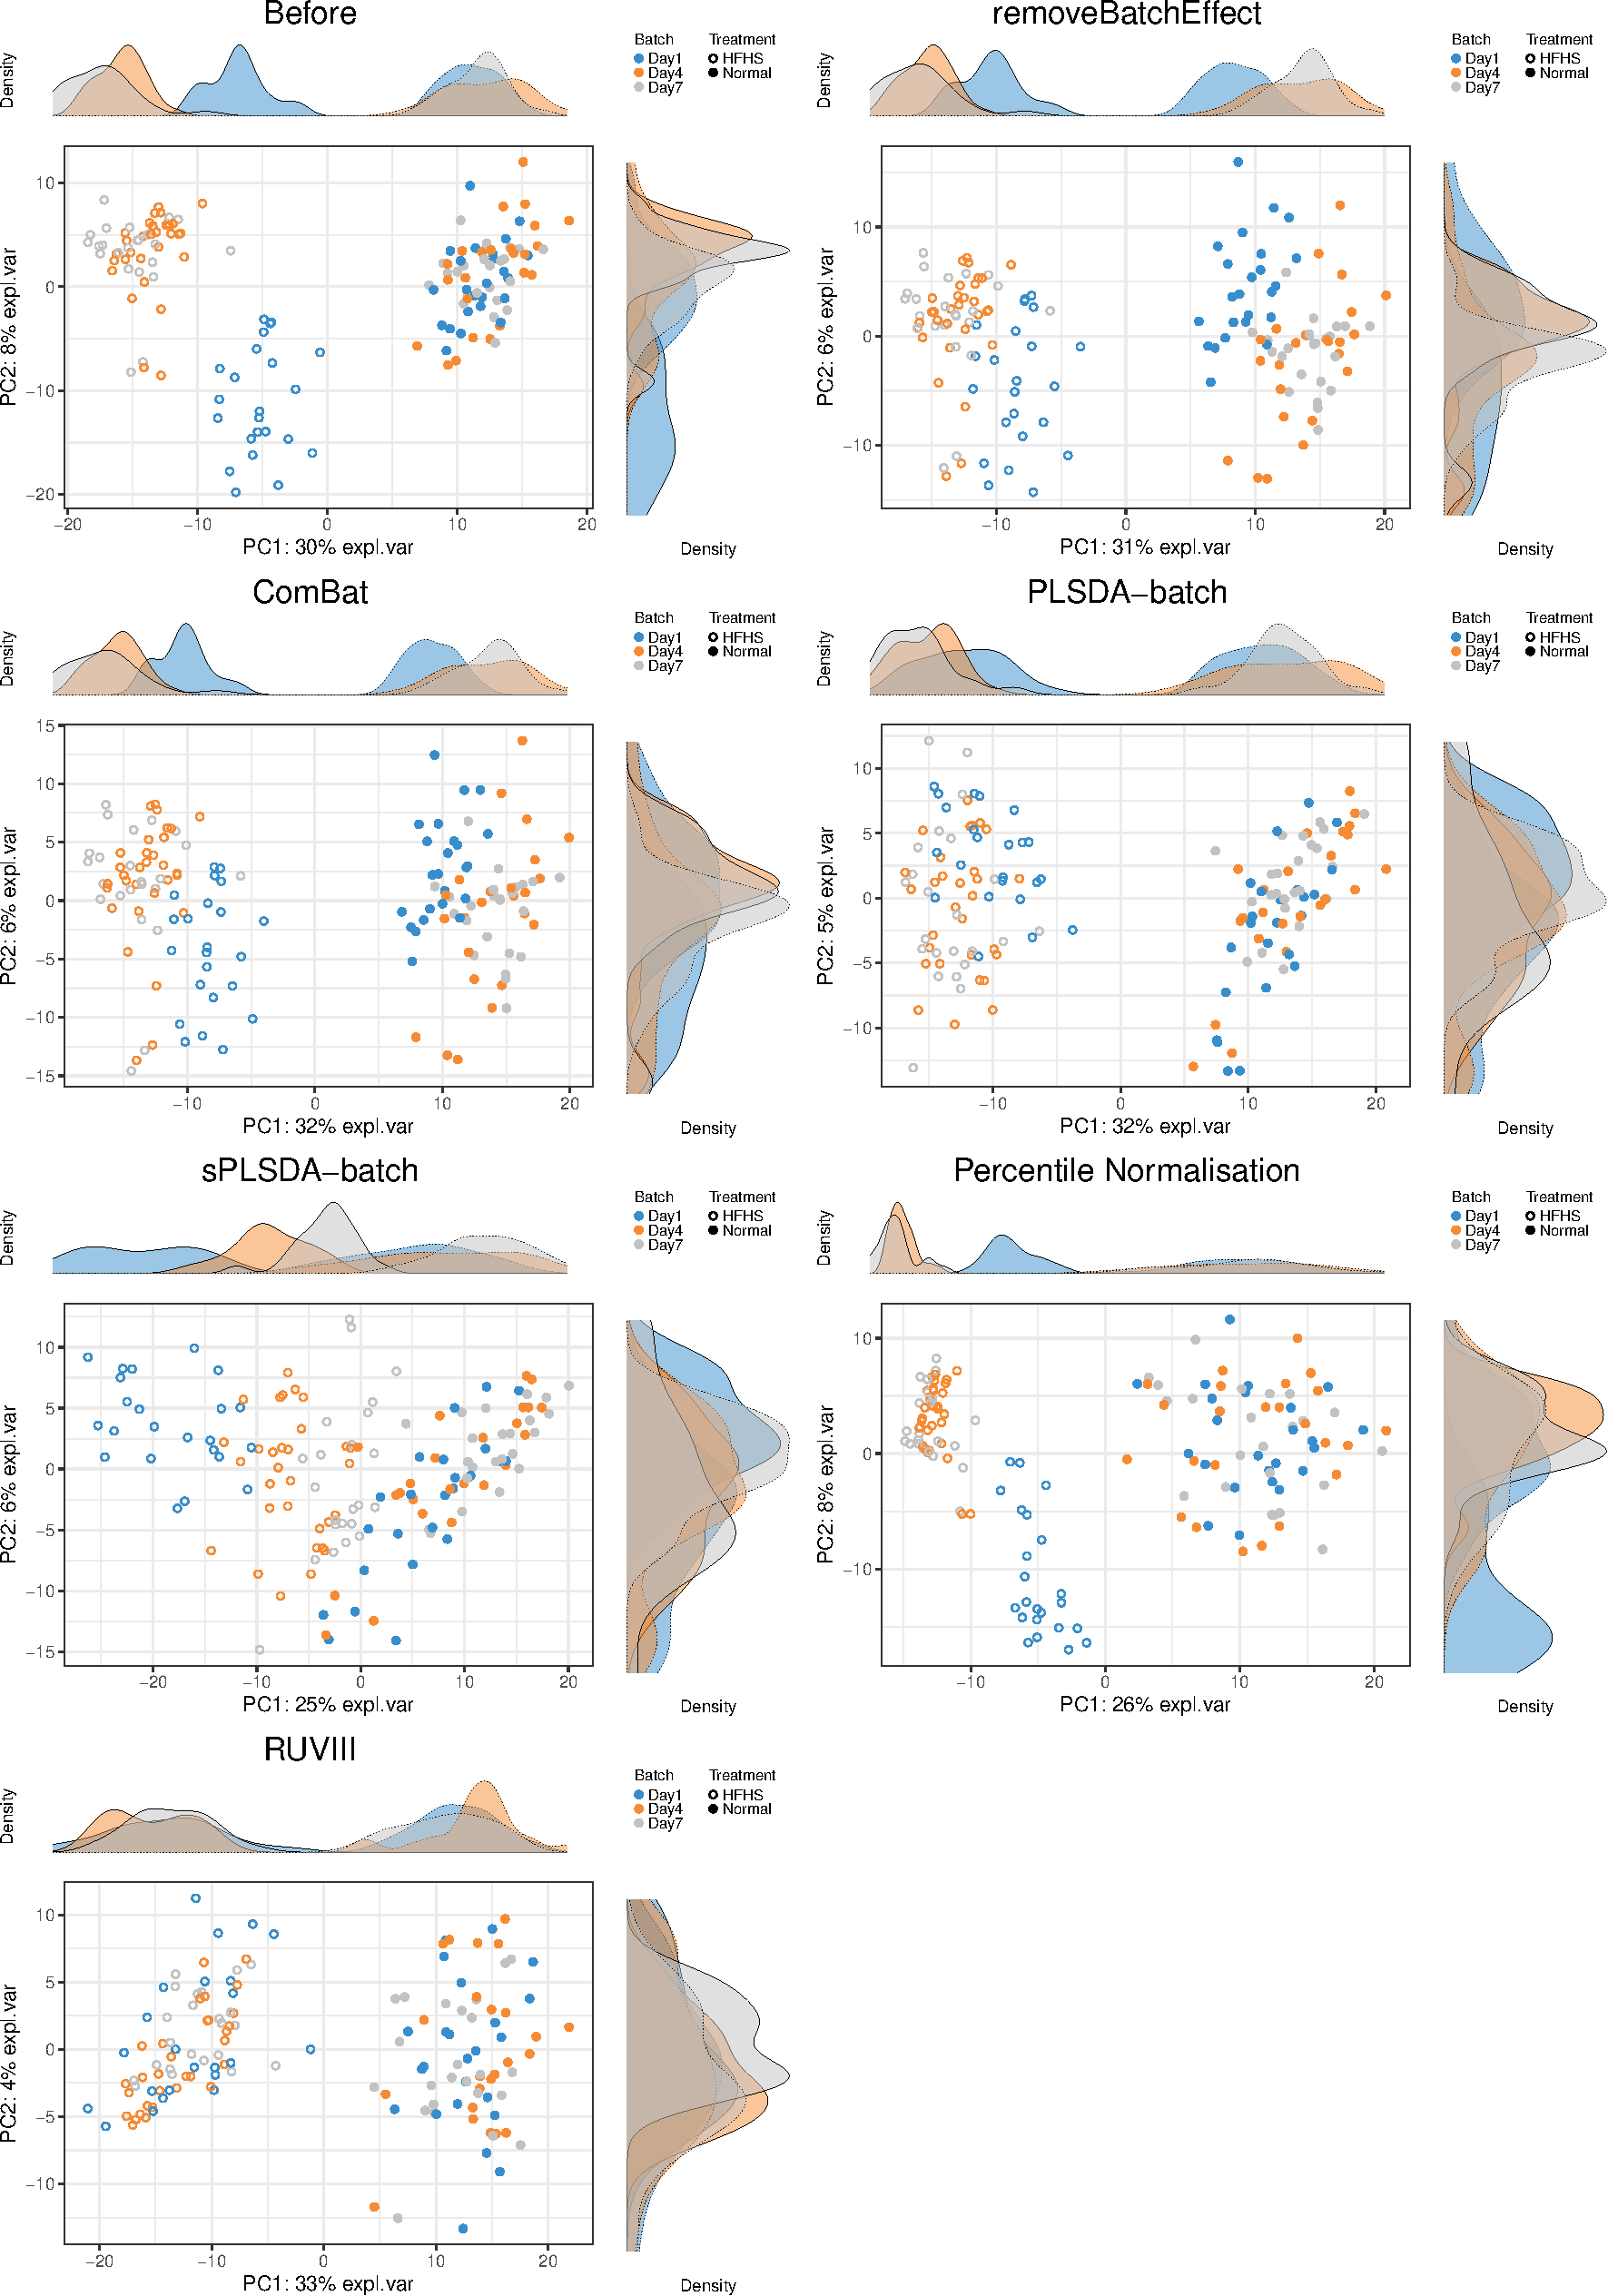
\includegraphics[width=1\linewidth]{PLSDAbatch_workflow_files/figure-latex/HFHSpca-1} 

}

\caption{The PCA sample plots with densities before and after batch effect correction in the HFHS data.}\label{fig:HFHSpca}
\end{figure}

In the above figures, the differences between the samples from different days were well removed after batch effect correction with PLSDA-batch and RUVIII. We can also compare the boxplots and density plots for key variables identified in PCA driving the major variance or in heatmaps showing obvious patterns before and after batch effect correction (results not shown).

\textbf{pRDA}

We calculate the global explained variance across all microbial variables using pRDA. To achieve this, we create a loop for each variable from the original (uncorrected) and batch effect-corrected data. The final results are then displayed with \texttt{partVar\_plot()} from \textcolor{orange}{PLSDAbatch} package.

\begin{Shaded}
\begin{Highlighting}[]
\CommentTok{\# HFHS data}
\NormalTok{hfhs.corrected.list }\OtherTok{\textless{}{-}} \FunctionTok{list}\NormalTok{(}\StringTok{\textasciigrave{}}\AttributeTok{Before correction}\StringTok{\textasciigrave{}} \OtherTok{=}\NormalTok{ hfhs.clr.less, }
                            \AttributeTok{removeBatchEffect =}\NormalTok{ hfhs.rBE, }
                            \AttributeTok{ComBat =}\NormalTok{ hfhs.ComBat, }
                            \StringTok{\textasciigrave{}}\AttributeTok{PLSDA{-}batch}\StringTok{\textasciigrave{}} \OtherTok{=}\NormalTok{ hfhs.PLSDA\_batch,}
                            \StringTok{\textasciigrave{}}\AttributeTok{sPLSDA{-}batch}\StringTok{\textasciigrave{}} \OtherTok{=}\NormalTok{ hfhs.sPLSDA\_batch, }
                            \StringTok{\textasciigrave{}}\AttributeTok{Percentile Normalisation}\StringTok{\textasciigrave{}} \OtherTok{=}\NormalTok{ hfhs.PN,}
                            \AttributeTok{RUVIII =}\NormalTok{ hfhs.RUVIII)}

\NormalTok{hfhs.prop.df }\OtherTok{\textless{}{-}} \FunctionTok{data.frame}\NormalTok{(}\AttributeTok{Treatment =} \ConstantTok{NA}\NormalTok{, }\AttributeTok{Batch =} \ConstantTok{NA}\NormalTok{, }
                           \AttributeTok{Intersection =} \ConstantTok{NA}\NormalTok{, }
                           \AttributeTok{Residuals =} \ConstantTok{NA}\NormalTok{) }
\ControlFlowTok{for}\NormalTok{(i }\ControlFlowTok{in} \DecValTok{1}\SpecialCharTok{:}\FunctionTok{length}\NormalTok{(hfhs.corrected.list))\{}
\NormalTok{  rda.res }\OtherTok{=} \FunctionTok{varpart}\NormalTok{(hfhs.corrected.list[[i]], }\SpecialCharTok{\textasciitilde{}}\NormalTok{ trt, }\SpecialCharTok{\textasciitilde{}}\NormalTok{ day,}
                    \AttributeTok{data =}\NormalTok{ hfhs.factors.df, }\AttributeTok{scale =}\NormalTok{ T)}
\NormalTok{  hfhs.prop.df[i, ] }\OtherTok{\textless{}{-}}\NormalTok{ rda.res}\SpecialCharTok{$}\NormalTok{part}\SpecialCharTok{$}\NormalTok{indfract}\SpecialCharTok{$}\NormalTok{Adj.R.squared\}}

\FunctionTok{rownames}\NormalTok{(hfhs.prop.df) }\OtherTok{=} \FunctionTok{names}\NormalTok{(hfhs.corrected.list)}

\NormalTok{hfhs.prop.df }\OtherTok{\textless{}{-}}\NormalTok{ hfhs.prop.df[, }\FunctionTok{c}\NormalTok{(}\DecValTok{1}\NormalTok{,}\DecValTok{3}\NormalTok{,}\DecValTok{2}\NormalTok{,}\DecValTok{4}\NormalTok{)]}

\NormalTok{hfhs.prop.df[hfhs.prop.df }\SpecialCharTok{\textless{}} \DecValTok{0}\NormalTok{] }\OtherTok{=} \DecValTok{0}
\NormalTok{hfhs.prop.df }\OtherTok{\textless{}{-}} \FunctionTok{as.data.frame}\NormalTok{(}\FunctionTok{t}\NormalTok{(}\FunctionTok{apply}\NormalTok{(hfhs.prop.df, }\DecValTok{1}\NormalTok{, }
                                      \ControlFlowTok{function}\NormalTok{(x)\{x}\SpecialCharTok{/}\FunctionTok{sum}\NormalTok{(x)\})))}


\FunctionTok{partVar\_plot}\NormalTok{(}\AttributeTok{prop.df =}\NormalTok{ hfhs.prop.df)}
\end{Highlighting}
\end{Shaded}

\begin{figure}

{\centering 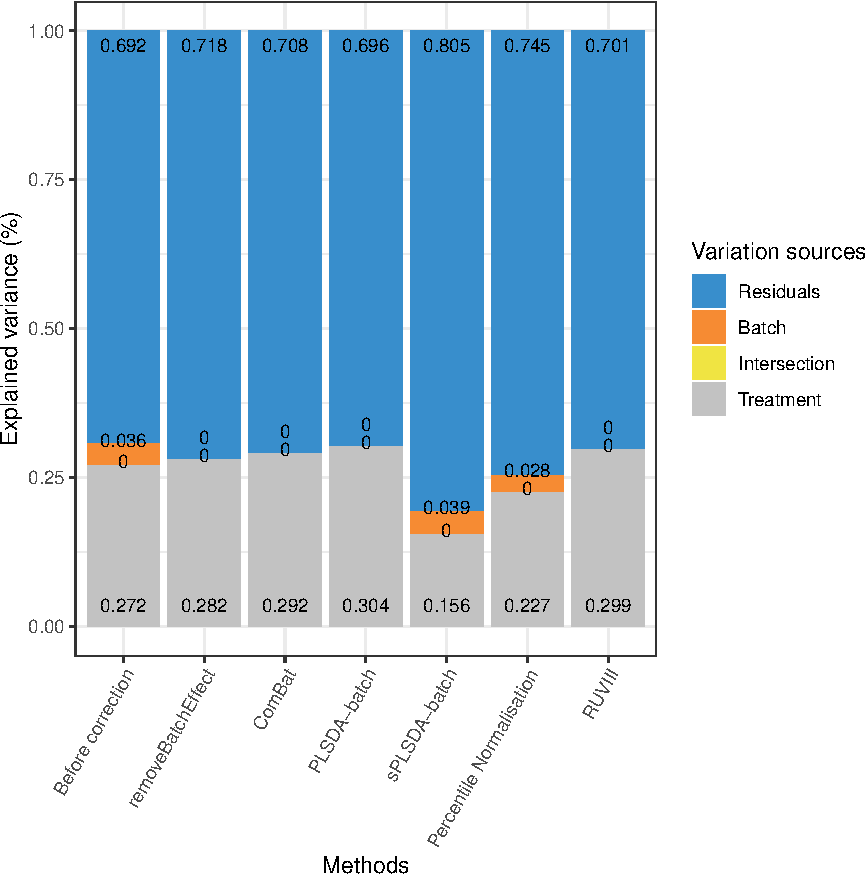
\includegraphics[width=0.6\linewidth]{PLSDAbatch_workflow_files/figure-latex/HFHSprdaSup-1} 

}

\caption{Global explained variance before and after batch effect correction for the HFHS data.}\label{fig:HFHSprdaSup}
\end{figure}

In the \textcolor{olive}{HFHS data}, a small amount of batch variance was observed (3.6\%) as shown in the above figure. PLSDA-batch achieved the best performance for preserving the largest treatment variance and completely removing batch variance compared to the other methods. The results also indicate that PLSDA-batch is more appropriate for weak batch effects, while sPLSDA-batch is more appropriate for strong batch effects. The RUVIII performed better in the \textcolor{olive}{HFHS data} than the \textcolor{blue}{AD data} because the sample replicates may help capturing more batch variation than in the \textcolor{blue}{AD data}. Indeed, the sample replicates in \textcolor{olive}{HFHS data} are across different day batches, while the replicates in \textcolor{blue}{AD data} do not exist in all batches. Therefore, sample replicates play a critical role in RUVIII.

\hypertarget{other-methods-2}{%
\subsubsection{Other methods}\label{other-methods-2}}

\textbf{\(R^2\)}

The \(R^2\) values for each variable are calculated with \texttt{lm()} from \textcolor{orange}{stats} package. To compare the \(R^2\) values among variables, we scale the corrected data before \(R^2\) calculation. The results are displayed with \texttt{ggplot()} from \textcolor{orange}{ggplot2} R package.

\begin{Shaded}
\begin{Highlighting}[]
\CommentTok{\# scale}
\NormalTok{hfhs.corr\_scale.list }\OtherTok{\textless{}{-}} \FunctionTok{lapply}\NormalTok{(hfhs.corrected.list, }
                               \ControlFlowTok{function}\NormalTok{(x)\{}\FunctionTok{apply}\NormalTok{(x, }\DecValTok{2}\NormalTok{, scale)\})}

\CommentTok{\# HFHS data}
\NormalTok{hfhs.r\_values.list }\OtherTok{\textless{}{-}} \FunctionTok{list}\NormalTok{()}
\ControlFlowTok{for}\NormalTok{(i }\ControlFlowTok{in} \DecValTok{1}\SpecialCharTok{:}\FunctionTok{length}\NormalTok{(hfhs.corr\_scale.list))\{}
\NormalTok{  hfhs.r\_values }\OtherTok{\textless{}{-}} \FunctionTok{data.frame}\NormalTok{(}\AttributeTok{trt =} \ConstantTok{NA}\NormalTok{, }\AttributeTok{batch =} \ConstantTok{NA}\NormalTok{)}
  \ControlFlowTok{for}\NormalTok{(c }\ControlFlowTok{in} \DecValTok{1}\SpecialCharTok{:}\FunctionTok{ncol}\NormalTok{(hfhs.corr\_scale.list[[i]]))\{}
\NormalTok{    hfhs.fit.res.trt }\OtherTok{\textless{}{-}} \FunctionTok{lm}\NormalTok{(hfhs.corr\_scale.list[[i]][,c] }\SpecialCharTok{\textasciitilde{}}\NormalTok{ hfhs.trt.less)}
\NormalTok{    hfhs.r\_values[c,}\DecValTok{1}\NormalTok{] }\OtherTok{\textless{}{-}} \FunctionTok{summary}\NormalTok{(hfhs.fit.res.trt)}\SpecialCharTok{$}\NormalTok{r.squared}
\NormalTok{    hfhs.fit.res.batch }\OtherTok{\textless{}{-}} \FunctionTok{lm}\NormalTok{(hfhs.corr\_scale.list[[i]][,c] }\SpecialCharTok{\textasciitilde{}}\NormalTok{ hfhs.day.less)}
\NormalTok{    hfhs.r\_values[c,}\DecValTok{2}\NormalTok{] }\OtherTok{\textless{}{-}} \FunctionTok{summary}\NormalTok{(hfhs.fit.res.batch)}\SpecialCharTok{$}\NormalTok{r.squared}
\NormalTok{  \}}
\NormalTok{  hfhs.r\_values.list[[i]] }\OtherTok{\textless{}{-}}\NormalTok{ hfhs.r\_values}
\NormalTok{\}}
\FunctionTok{names}\NormalTok{(hfhs.r\_values.list) }\OtherTok{\textless{}{-}} \FunctionTok{names}\NormalTok{(hfhs.corr\_scale.list)}

\NormalTok{hfhs.boxp.list }\OtherTok{\textless{}{-}} \FunctionTok{list}\NormalTok{()}
\ControlFlowTok{for}\NormalTok{(i }\ControlFlowTok{in} \FunctionTok{seq\_len}\NormalTok{(}\FunctionTok{length}\NormalTok{(hfhs.r\_values.list)))\{}
\NormalTok{  hfhs.boxp.list[[i]] }\OtherTok{\textless{}{-}} 
    \FunctionTok{data.frame}\NormalTok{(}\AttributeTok{r2 =} \FunctionTok{c}\NormalTok{(hfhs.r\_values.list[[i]][ ,}\StringTok{\textquotesingle{}trt\textquotesingle{}}\NormalTok{],}
\NormalTok{                      hfhs.r\_values.list[[i]][ ,}\StringTok{\textquotesingle{}batch\textquotesingle{}}\NormalTok{]), }
               \AttributeTok{Effects =} \FunctionTok{as.factor}\NormalTok{(}\FunctionTok{rep}\NormalTok{(}\FunctionTok{c}\NormalTok{(}\StringTok{\textquotesingle{}Treatment\textquotesingle{}}\NormalTok{,}\StringTok{\textquotesingle{}Batch\textquotesingle{}}\NormalTok{), }
                                       \AttributeTok{each =} \DecValTok{515}\NormalTok{)))}
\NormalTok{\}}
\FunctionTok{names}\NormalTok{(hfhs.boxp.list) }\OtherTok{\textless{}{-}} \FunctionTok{names}\NormalTok{(hfhs.r\_values.list)}

\NormalTok{hfhs.r2.boxp }\OtherTok{\textless{}{-}} \FunctionTok{rbind}\NormalTok{(hfhs.boxp.list}\SpecialCharTok{$}\StringTok{\textasciigrave{}}\AttributeTok{Before correction}\StringTok{\textasciigrave{}}\NormalTok{,}
\NormalTok{                      hfhs.boxp.list}\SpecialCharTok{$}\NormalTok{removeBatchEffect,}
\NormalTok{                      hfhs.boxp.list}\SpecialCharTok{$}\NormalTok{ComBat,}
\NormalTok{                      hfhs.boxp.list}\SpecialCharTok{$}\StringTok{\textasciigrave{}}\AttributeTok{PLSDA{-}batch}\StringTok{\textasciigrave{}}\NormalTok{,}
\NormalTok{                      hfhs.boxp.list}\SpecialCharTok{$}\StringTok{\textasciigrave{}}\AttributeTok{sPLSDA{-}batch}\StringTok{\textasciigrave{}}\NormalTok{,}
\NormalTok{                      hfhs.boxp.list}\SpecialCharTok{$}\StringTok{\textasciigrave{}}\AttributeTok{Percentile Normalisation}\StringTok{\textasciigrave{}}\NormalTok{,}
\NormalTok{                      hfhs.boxp.list}\SpecialCharTok{$}\NormalTok{RUVIII)}

\NormalTok{hfhs.r2.boxp}\SpecialCharTok{$}\NormalTok{methods }\OtherTok{\textless{}{-}} \FunctionTok{rep}\NormalTok{(}\FunctionTok{c}\NormalTok{(}\StringTok{\textquotesingle{}Before correction\textquotesingle{}}\NormalTok{, }\StringTok{\textquotesingle{} removeBatchEffect\textquotesingle{}}\NormalTok{, }
                              \StringTok{\textquotesingle{}ComBat\textquotesingle{}}\NormalTok{,}\StringTok{\textquotesingle{}PLSDA{-}batch\textquotesingle{}}\NormalTok{, }\StringTok{\textquotesingle{}sPLSDA{-}batch\textquotesingle{}}\NormalTok{,}
                              \StringTok{\textquotesingle{}Percentile Normalisation\textquotesingle{}}\NormalTok{, }\StringTok{\textquotesingle{}RUVIII\textquotesingle{}}\NormalTok{), }
                            \AttributeTok{each =} \DecValTok{1030}\NormalTok{)}

\NormalTok{hfhs.r2.boxp}\SpecialCharTok{$}\NormalTok{methods }\OtherTok{\textless{}{-}} \FunctionTok{factor}\NormalTok{(hfhs.r2.boxp}\SpecialCharTok{$}\NormalTok{methods, }
                               \AttributeTok{levels =} \FunctionTok{unique}\NormalTok{(hfhs.r2.boxp}\SpecialCharTok{$}\NormalTok{methods))}

\FunctionTok{ggplot}\NormalTok{(hfhs.r2.boxp, }\FunctionTok{aes}\NormalTok{(}\AttributeTok{x =}\NormalTok{ Effects, }\AttributeTok{y =}\NormalTok{ r2, }\AttributeTok{fill =}\NormalTok{ Effects)) }\SpecialCharTok{+}
  \FunctionTok{geom\_boxplot}\NormalTok{(}\AttributeTok{alpha =} \FloatTok{0.80}\NormalTok{) }\SpecialCharTok{+}
  \FunctionTok{theme\_bw}\NormalTok{() }\SpecialCharTok{+} 
  \FunctionTok{theme}\NormalTok{(}\AttributeTok{text =} \FunctionTok{element\_text}\NormalTok{(}\AttributeTok{size =} \DecValTok{18}\NormalTok{),}
        \AttributeTok{axis.title.x =} \FunctionTok{element\_blank}\NormalTok{(),}
        \AttributeTok{axis.title.y =} \FunctionTok{element\_blank}\NormalTok{(),}
        \AttributeTok{axis.text.x =} \FunctionTok{element\_text}\NormalTok{(}\AttributeTok{angle =} \DecValTok{60}\NormalTok{, }\AttributeTok{hjust =} \DecValTok{1}\NormalTok{, }\AttributeTok{size =} \DecValTok{18}\NormalTok{),}
        \AttributeTok{axis.text.y =} \FunctionTok{element\_text}\NormalTok{(}\AttributeTok{size =} \DecValTok{18}\NormalTok{),}
        \AttributeTok{panel.grid.minor.x =} \FunctionTok{element\_blank}\NormalTok{(),}
        \AttributeTok{panel.grid.major.x =} \FunctionTok{element\_blank}\NormalTok{(),}
        \AttributeTok{legend.position =} \StringTok{"right"}\NormalTok{) }\SpecialCharTok{+} \FunctionTok{facet\_grid}\NormalTok{( }\SpecialCharTok{\textasciitilde{}}\NormalTok{ methods) }\SpecialCharTok{+} 
  \FunctionTok{scale\_fill\_manual}\NormalTok{(}\AttributeTok{values=}\FunctionTok{pb\_color}\NormalTok{(}\FunctionTok{c}\NormalTok{(}\DecValTok{12}\NormalTok{,}\DecValTok{14}\NormalTok{))) }
\end{Highlighting}
\end{Shaded}

\begin{figure}

{\centering \includegraphics[width=1\linewidth]{PLSDAbatch_workflow_files/figure-latex/HFHSr21-1} 

}

\caption{HFHS study: $R^2$ values for each microbial variable before and after batch effect correction.}\label{fig:HFHSr21}
\end{figure}

We observed from these plots that the data corrected by sPLSDA-batch, percentile normalisation still included many variables with a large proportion of batch variance.

\begin{Shaded}
\begin{Highlighting}[]
\DocumentationTok{\#\#\#\#\#\#\#\#\#\#\#\#\#\#\#\#\#\#\#\#\#\#\#\#\#\#\#\#\#\#\#\#\#\#}
\NormalTok{hfhs.barp.list }\OtherTok{\textless{}{-}} \FunctionTok{list}\NormalTok{()}
\ControlFlowTok{for}\NormalTok{(i }\ControlFlowTok{in} \FunctionTok{seq\_len}\NormalTok{(}\FunctionTok{length}\NormalTok{(hfhs.r\_values.list)))\{}
\NormalTok{  hfhs.barp.list[[i]] }\OtherTok{\textless{}{-}} 
    \FunctionTok{data.frame}\NormalTok{(}\AttributeTok{r2 =} \FunctionTok{c}\NormalTok{(}\FunctionTok{sum}\NormalTok{(hfhs.r\_values.list[[i]][ ,}\StringTok{\textquotesingle{}trt\textquotesingle{}}\NormalTok{]),}
                      \FunctionTok{sum}\NormalTok{(hfhs.r\_values.list[[i]][ ,}\StringTok{\textquotesingle{}batch\textquotesingle{}}\NormalTok{])), }
               \AttributeTok{Effects =} \FunctionTok{c}\NormalTok{(}\StringTok{\textquotesingle{}Treatment\textquotesingle{}}\NormalTok{,}\StringTok{\textquotesingle{}Batch\textquotesingle{}}\NormalTok{))}
\NormalTok{\}}
\FunctionTok{names}\NormalTok{(hfhs.barp.list) }\OtherTok{\textless{}{-}} \FunctionTok{names}\NormalTok{(hfhs.r\_values.list)}

\NormalTok{hfhs.r2.barp }\OtherTok{\textless{}{-}} \FunctionTok{rbind}\NormalTok{(hfhs.barp.list}\SpecialCharTok{$}\StringTok{\textasciigrave{}}\AttributeTok{Before correction}\StringTok{\textasciigrave{}}\NormalTok{,}
\NormalTok{                      hfhs.barp.list}\SpecialCharTok{$}\NormalTok{removeBatchEffect,}
\NormalTok{                      hfhs.barp.list}\SpecialCharTok{$}\NormalTok{ComBat,}
\NormalTok{                      hfhs.barp.list}\SpecialCharTok{$}\StringTok{\textasciigrave{}}\AttributeTok{PLSDA{-}batch}\StringTok{\textasciigrave{}}\NormalTok{,}
\NormalTok{                      hfhs.barp.list}\SpecialCharTok{$}\StringTok{\textasciigrave{}}\AttributeTok{sPLSDA{-}batch}\StringTok{\textasciigrave{}}\NormalTok{,}
\NormalTok{                      hfhs.barp.list}\SpecialCharTok{$}\StringTok{\textasciigrave{}}\AttributeTok{Percentile Normalisation}\StringTok{\textasciigrave{}}\NormalTok{,}
\NormalTok{                      hfhs.barp.list}\SpecialCharTok{$}\NormalTok{RUVIII)}


\NormalTok{hfhs.r2.barp}\SpecialCharTok{$}\NormalTok{methods }\OtherTok{\textless{}{-}} \FunctionTok{rep}\NormalTok{(}\FunctionTok{c}\NormalTok{(}\StringTok{\textquotesingle{}Before correction\textquotesingle{}}\NormalTok{, }\StringTok{\textquotesingle{} removeBatchEffect\textquotesingle{}}\NormalTok{, }
                              \StringTok{\textquotesingle{}ComBat\textquotesingle{}}\NormalTok{,}\StringTok{\textquotesingle{}PLSDA{-}batch\textquotesingle{}}\NormalTok{, }\StringTok{\textquotesingle{}sPLSDA{-}batch\textquotesingle{}}\NormalTok{,}
                              \StringTok{\textquotesingle{}Percentile Normalisation\textquotesingle{}}\NormalTok{, }\StringTok{\textquotesingle{}RUVIII\textquotesingle{}}\NormalTok{), }\AttributeTok{each =} \DecValTok{2}\NormalTok{)}

\NormalTok{hfhs.r2.barp}\SpecialCharTok{$}\NormalTok{methods }\OtherTok{\textless{}{-}} \FunctionTok{factor}\NormalTok{(hfhs.r2.barp}\SpecialCharTok{$}\NormalTok{methods, }
                               \AttributeTok{levels =} \FunctionTok{unique}\NormalTok{(hfhs.r2.barp}\SpecialCharTok{$}\NormalTok{methods))}


\FunctionTok{ggplot}\NormalTok{(hfhs.r2.barp, }\FunctionTok{aes}\NormalTok{(}\AttributeTok{x =}\NormalTok{ Effects, }\AttributeTok{y =}\NormalTok{ r2, }\AttributeTok{fill =}\NormalTok{ Effects)) }\SpecialCharTok{+}
  \FunctionTok{geom\_bar}\NormalTok{(}\AttributeTok{stat=}\StringTok{"identity"}\NormalTok{) }\SpecialCharTok{+} 
  \FunctionTok{theme\_bw}\NormalTok{() }\SpecialCharTok{+} 
  \FunctionTok{theme}\NormalTok{(}\AttributeTok{text =} \FunctionTok{element\_text}\NormalTok{(}\AttributeTok{size =} \DecValTok{18}\NormalTok{),}
        \AttributeTok{axis.title.x =} \FunctionTok{element\_blank}\NormalTok{(),}
        \AttributeTok{axis.title.y =} \FunctionTok{element\_blank}\NormalTok{(),}
        \AttributeTok{axis.text.x =} \FunctionTok{element\_text}\NormalTok{(}\AttributeTok{angle =} \DecValTok{60}\NormalTok{, }\AttributeTok{hjust =} \DecValTok{1}\NormalTok{, }\AttributeTok{size =} \DecValTok{18}\NormalTok{),}
        \AttributeTok{axis.text.y =} \FunctionTok{element\_text}\NormalTok{(}\AttributeTok{size =} \DecValTok{18}\NormalTok{),}
        \AttributeTok{panel.grid.minor.x =} \FunctionTok{element\_blank}\NormalTok{(),}
        \AttributeTok{panel.grid.major.x =} \FunctionTok{element\_blank}\NormalTok{(),}
        \AttributeTok{legend.position =} \StringTok{"right"}\NormalTok{) }\SpecialCharTok{+} \FunctionTok{facet\_grid}\NormalTok{( }\SpecialCharTok{\textasciitilde{}}\NormalTok{ methods) }\SpecialCharTok{+} 
  \FunctionTok{scale\_fill\_manual}\NormalTok{(}\AttributeTok{values=}\FunctionTok{pb\_color}\NormalTok{(}\FunctionTok{c}\NormalTok{(}\DecValTok{12}\NormalTok{,}\DecValTok{14}\NormalTok{)))}
\end{Highlighting}
\end{Shaded}

\begin{figure}

{\centering 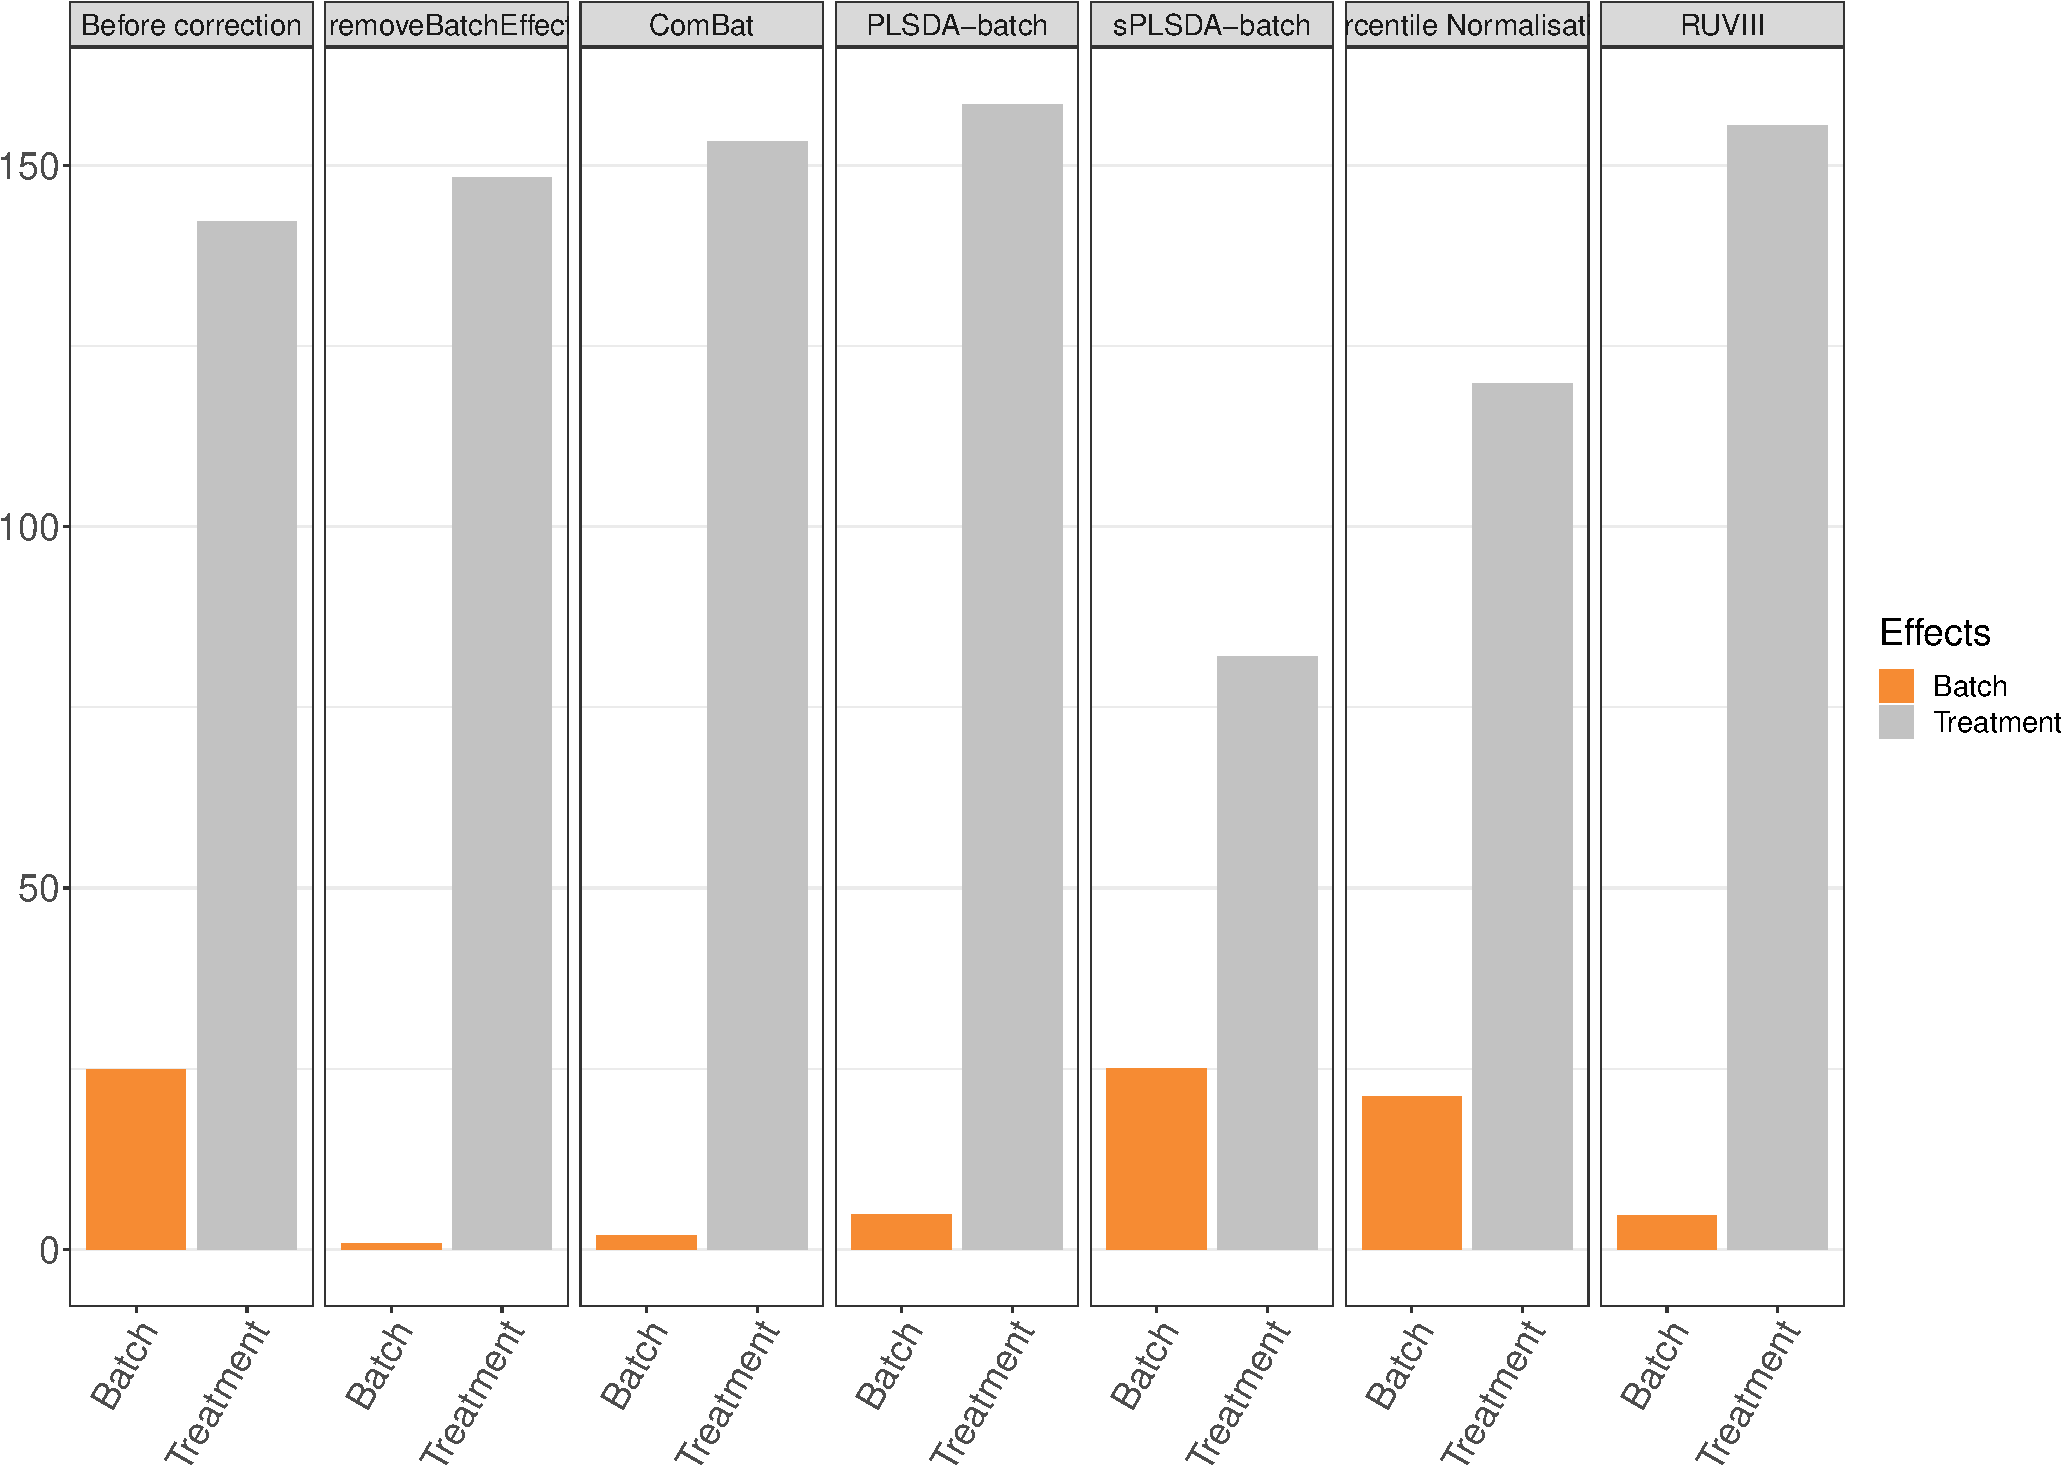
\includegraphics[width=1\linewidth]{PLSDAbatch_workflow_files/figure-latex/HFHSr22-1} 

}

\caption{HFHS study: the sum of $R^2$ values for each microbial variable before and after batch effect correction.}\label{fig:HFHSr22}
\end{figure}

When considering the sum of all variables, the remaining batch variance of corrected data from PLSDA-batch is greater than removeBatchEffect, ComBat and RUVIII. The preserved treatment variance of corrected data from PLSDA-batch is the largest.

\textbf{Alignment scores}

We use the \texttt{alignment\_score()} function from \textcolor{orange}{PLSDAbatch}. We need to specify the proportion of data variance to explain (\texttt{var}), the number of nearest neighbours (\texttt{k}) and the number of principal components to estimate (\texttt{ncomp}). We then use \texttt{ggplot()} function from \textcolor{orange}{ggplot2} to visualise the results.

\begin{Shaded}
\begin{Highlighting}[]
\CommentTok{\# HFHS data}
\NormalTok{hfhs.var }\OtherTok{=} \FloatTok{0.95}
\NormalTok{hfhs.k }\OtherTok{=} \DecValTok{15}

\NormalTok{hfhs.scores }\OtherTok{\textless{}{-}} \FunctionTok{c}\NormalTok{()}
\ControlFlowTok{for}\NormalTok{(i }\ControlFlowTok{in} \DecValTok{1}\SpecialCharTok{:}\FunctionTok{length}\NormalTok{(hfhs.corrected.list))\{}
\NormalTok{  res }\OtherTok{\textless{}{-}} \FunctionTok{alignment\_score}\NormalTok{(}\AttributeTok{data =}\NormalTok{ hfhs.corrected.list[[i]], }
                         \AttributeTok{batch =}\NormalTok{ hfhs.day.less, }
                         \AttributeTok{var =}\NormalTok{ hfhs.var, }
                         \AttributeTok{k =}\NormalTok{ hfhs.k, }
                         \AttributeTok{ncomp =} \DecValTok{130}\NormalTok{)}
\NormalTok{  hfhs.scores }\OtherTok{\textless{}{-}} \FunctionTok{c}\NormalTok{(hfhs.scores, res)}
\NormalTok{\}}

\NormalTok{hfhs.scores.df }\OtherTok{\textless{}{-}} \FunctionTok{data.frame}\NormalTok{(}\AttributeTok{scores =}\NormalTok{ hfhs.scores, }
                             \AttributeTok{methods =} \FunctionTok{names}\NormalTok{(hfhs.corrected.list))}

\NormalTok{hfhs.scores.df}\SpecialCharTok{$}\NormalTok{methods }\OtherTok{\textless{}{-}} \FunctionTok{factor}\NormalTok{(hfhs.scores.df}\SpecialCharTok{$}\NormalTok{methods, }
                                 \AttributeTok{levels =} \FunctionTok{rev}\NormalTok{(}\FunctionTok{names}\NormalTok{(hfhs.corrected.list)))}


\FunctionTok{ggplot}\NormalTok{() }\SpecialCharTok{+} \FunctionTok{geom\_col}\NormalTok{(}\FunctionTok{aes}\NormalTok{(}\AttributeTok{x =}\NormalTok{ hfhs.scores.df}\SpecialCharTok{$}\NormalTok{methods, }
                        \AttributeTok{y =}\NormalTok{ hfhs.scores.df}\SpecialCharTok{$}\NormalTok{scores)) }\SpecialCharTok{+} 
  \FunctionTok{geom\_text}\NormalTok{(}\FunctionTok{aes}\NormalTok{(}\AttributeTok{x =}\NormalTok{ hfhs.scores.df}\SpecialCharTok{$}\NormalTok{methods, }
                \AttributeTok{y =}\NormalTok{ hfhs.scores.df}\SpecialCharTok{$}\NormalTok{scores}\SpecialCharTok{/}\DecValTok{2}\NormalTok{, }
                \AttributeTok{label =} \FunctionTok{round}\NormalTok{(hfhs.scores.df}\SpecialCharTok{$}\NormalTok{scores, }\DecValTok{3}\NormalTok{)), }
            \AttributeTok{size =} \DecValTok{3}\NormalTok{, }\AttributeTok{col =} \StringTok{\textquotesingle{}white\textquotesingle{}}\NormalTok{) }\SpecialCharTok{+} 
  \FunctionTok{coord\_flip}\NormalTok{() }\SpecialCharTok{+} \FunctionTok{theme\_bw}\NormalTok{() }\SpecialCharTok{+} \FunctionTok{ylab}\NormalTok{(}\StringTok{\textquotesingle{}Alignment Scores\textquotesingle{}}\NormalTok{) }\SpecialCharTok{+} 
  \FunctionTok{xlab}\NormalTok{(}\StringTok{\textquotesingle{}\textquotesingle{}}\NormalTok{) }\SpecialCharTok{+} \FunctionTok{ylim}\NormalTok{(}\DecValTok{0}\NormalTok{,}\FloatTok{0.85}\NormalTok{)}
\end{Highlighting}
\end{Shaded}

\begin{figure}

{\centering 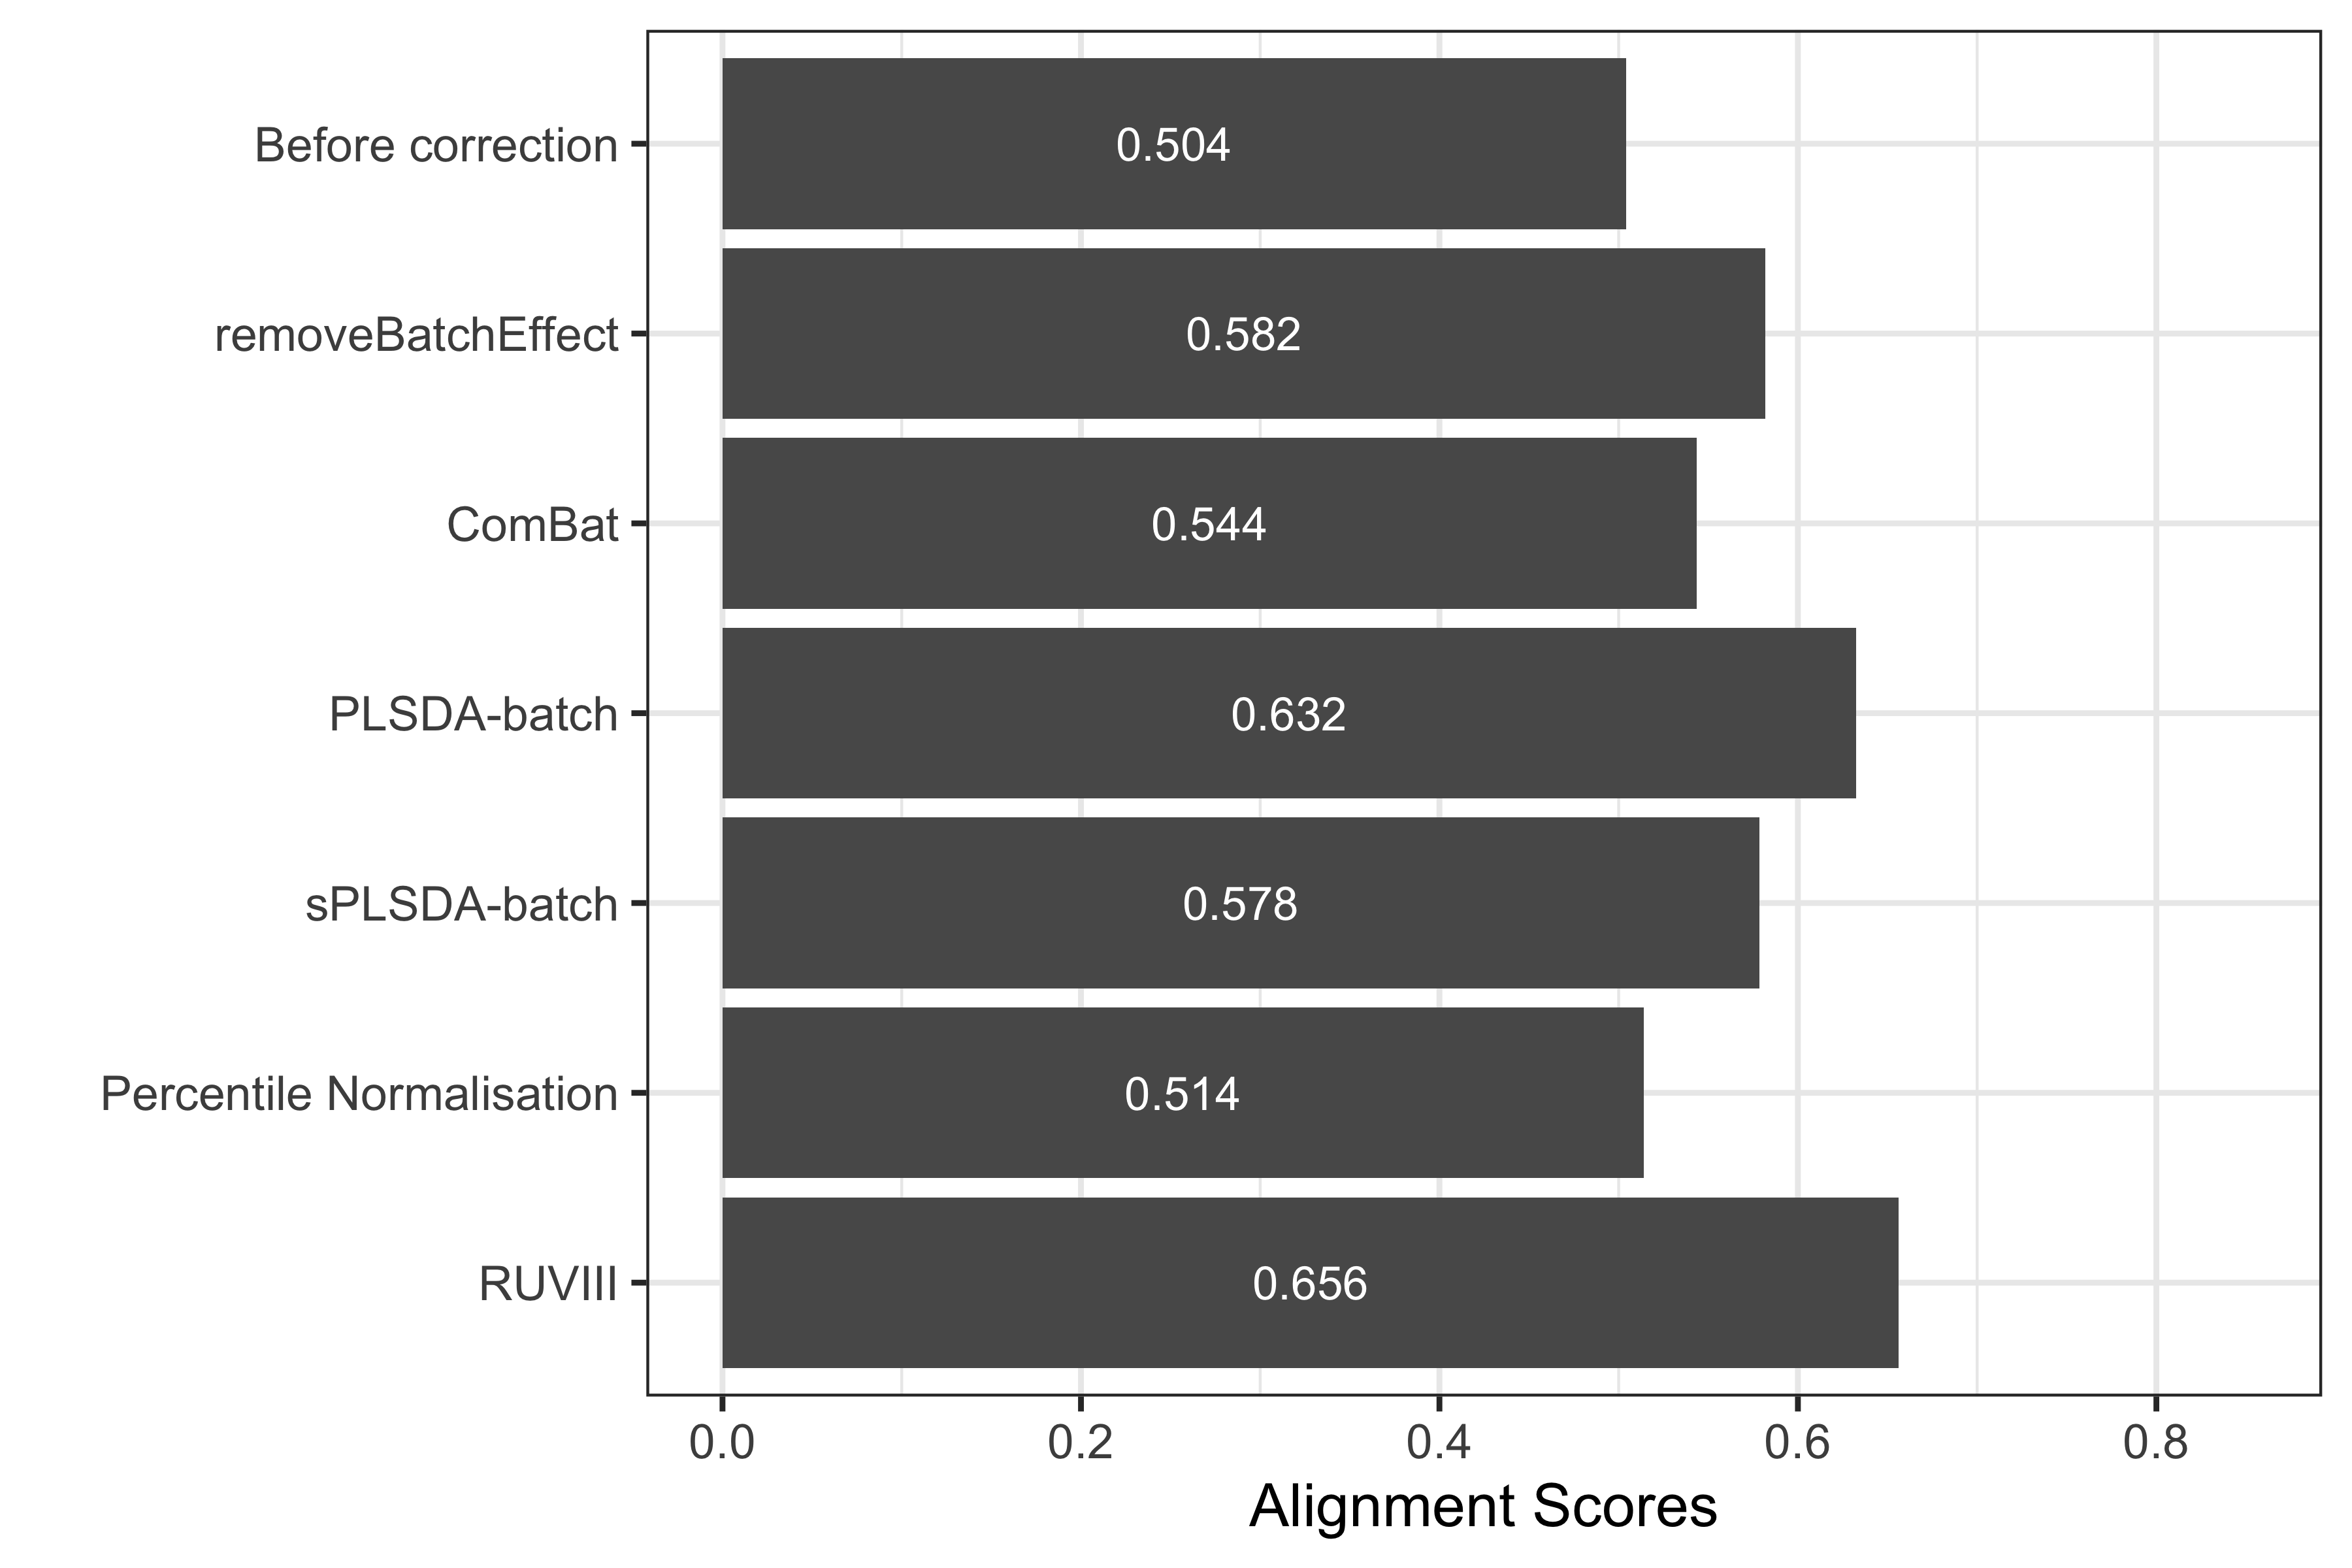
\includegraphics[width=0.6\linewidth]{PLSDAbatch_workflow_files/figure-latex/HFHSalignment-1} 

}

\caption{Comparison of alignment scores before and after batch effect correction using different methods for the HFHS data.}\label{fig:HFHSalignment}
\end{figure}

The alignment scores complement the PCA results, especially when batch effect removal is difficult to assess on PCA sample plots. For example in the PCA plots for the \textcolor{olive}{HFHS data}, we observed that the samples across different batches were better mixed after batch effect correction with PLSDA-batch and RUVIII than before, while the performance of these two methods was difficult to compare. Since a higher alignment score indicates that samples are better mixed, as shown in the above figure, RUVIII gave a superior performance compared to the other methods.

We recommend the sparse version of PLSDA-batch for a very strong batch effect, for example, in the \textcolor{blue}{AD data}. However, for a weak batch effect, we do not recommend removing batch effects in the \textcolor{olive}{HFHS data}, but if we have to, we recommend using PLSDA-batch. It is easier to lose treatment variation when the batch variation is very small. Therefore PLSDA-batch can better ensure the complete preservation of treatment variation than a sparse version.

\textbf{Variable selection}

We use \texttt{splsda()} from \textcolor{orange}{mixOmics} to select the top 50 microbial variables that, in combination, discriminate the different treatment groups in the \textcolor{olive}{HFHS data}. We apply \texttt{splsda()} to the different batch effect corrected data from all methods. Then we use \texttt{upset()} from \textcolor{orange}{UpSetR} package \citep{lex2014upset} to visualise the concordance of variables selected.

In the code below, we first need to convert the list of variables selected from different method-corrected data into a data frame compatible with \texttt{upset()} using \texttt{fromList()}. We then assign different colour schemes for each variable selection.

\begin{Shaded}
\begin{Highlighting}[]
\NormalTok{hfhs.splsda.select }\OtherTok{\textless{}{-}} \FunctionTok{list}\NormalTok{()}
\ControlFlowTok{for}\NormalTok{(i }\ControlFlowTok{in} \DecValTok{1}\SpecialCharTok{:}\FunctionTok{length}\NormalTok{(hfhs.corrected.list))\{}
\NormalTok{  splsda.res }\OtherTok{\textless{}{-}} \FunctionTok{splsda}\NormalTok{(}\AttributeTok{X =}\NormalTok{ hfhs.corrected.list[[i]],}
                       \AttributeTok{Y =}\NormalTok{ hfhs.trt.less, }
                       \AttributeTok{ncomp =} \DecValTok{3}\NormalTok{, }\AttributeTok{keepX =} \FunctionTok{rep}\NormalTok{(}\DecValTok{50}\NormalTok{,}\DecValTok{3}\NormalTok{))}
\NormalTok{  select.res }\OtherTok{\textless{}{-}} \FunctionTok{selectVar}\NormalTok{(splsda.res, }\AttributeTok{comp =} \DecValTok{1}\NormalTok{)}\SpecialCharTok{$}\NormalTok{name}
\NormalTok{  hfhs.splsda.select[[i]] }\OtherTok{\textless{}{-}}\NormalTok{ select.res}
\NormalTok{\}}
\FunctionTok{names}\NormalTok{(hfhs.splsda.select) }\OtherTok{\textless{}{-}} \FunctionTok{names}\NormalTok{(hfhs.corrected.list)}

\CommentTok{\# can only visualise 5 methods}
\NormalTok{hfhs.splsda.select }\OtherTok{\textless{}{-}}\NormalTok{ hfhs.splsda.select[}\FunctionTok{c}\NormalTok{(}\DecValTok{1}\SpecialCharTok{:}\DecValTok{4}\NormalTok{,}\DecValTok{7}\NormalTok{)]}

\NormalTok{hfhs.splsda.upsetR }\OtherTok{\textless{}{-}} \FunctionTok{fromList}\NormalTok{(hfhs.splsda.select)}

\FunctionTok{upset}\NormalTok{(hfhs.splsda.upsetR, }\AttributeTok{main.bar.color =} \StringTok{\textquotesingle{}gray36\textquotesingle{}}\NormalTok{,}
      \AttributeTok{sets.bar.color =} \FunctionTok{pb\_color}\NormalTok{(}\FunctionTok{c}\NormalTok{(}\DecValTok{25}\SpecialCharTok{:}\DecValTok{22}\NormalTok{,}\DecValTok{20}\NormalTok{)), }\AttributeTok{matrix.color =} \StringTok{\textquotesingle{}gray36\textquotesingle{}}\NormalTok{,}
      \AttributeTok{order.by =} \StringTok{\textquotesingle{}freq\textquotesingle{}}\NormalTok{, }\AttributeTok{empty.intersections =} \StringTok{\textquotesingle{}on\textquotesingle{}}\NormalTok{,}
      \AttributeTok{queries =} 
        \FunctionTok{list}\NormalTok{(}\FunctionTok{list}\NormalTok{(}\AttributeTok{query =}\NormalTok{ intersects, }\AttributeTok{params =} \FunctionTok{list}\NormalTok{(}\StringTok{\textquotesingle{}Before correction\textquotesingle{}}\NormalTok{), }
                  \AttributeTok{color =} \FunctionTok{pb\_color}\NormalTok{(}\DecValTok{20}\NormalTok{), }\AttributeTok{active =}\NormalTok{ T),}
             \FunctionTok{list}\NormalTok{(}\AttributeTok{query =}\NormalTok{ intersects, }\AttributeTok{params =} \FunctionTok{list}\NormalTok{(}\StringTok{\textquotesingle{}removeBatchEffect\textquotesingle{}}\NormalTok{), }
                  \AttributeTok{color =} \FunctionTok{pb\_color}\NormalTok{(}\DecValTok{22}\NormalTok{), }\AttributeTok{active =}\NormalTok{ T),}
             \FunctionTok{list}\NormalTok{(}\AttributeTok{query =}\NormalTok{ intersects, }\AttributeTok{params =} \FunctionTok{list}\NormalTok{(}\StringTok{\textquotesingle{}ComBat\textquotesingle{}}\NormalTok{), }
                  \AttributeTok{color =} \FunctionTok{pb\_color}\NormalTok{(}\DecValTok{23}\NormalTok{), }\AttributeTok{active =}\NormalTok{ T),}
             \FunctionTok{list}\NormalTok{(}\AttributeTok{query =}\NormalTok{ intersects, }\AttributeTok{params =} \FunctionTok{list}\NormalTok{(}\StringTok{\textquotesingle{}PLSDA{-}batch\textquotesingle{}}\NormalTok{), }
                  \AttributeTok{color =} \FunctionTok{pb\_color}\NormalTok{(}\DecValTok{24}\NormalTok{), }\AttributeTok{active =}\NormalTok{ T),}
             \FunctionTok{list}\NormalTok{(}\AttributeTok{query =}\NormalTok{ intersects, }\AttributeTok{params =} \FunctionTok{list}\NormalTok{(}\StringTok{\textquotesingle{}RUVIII\textquotesingle{}}\NormalTok{), }
                  \AttributeTok{color =} \FunctionTok{pb\_color}\NormalTok{(}\DecValTok{25}\NormalTok{), }\AttributeTok{active =}\NormalTok{ T)))}
\end{Highlighting}
\end{Shaded}

\begin{figure}

{\centering 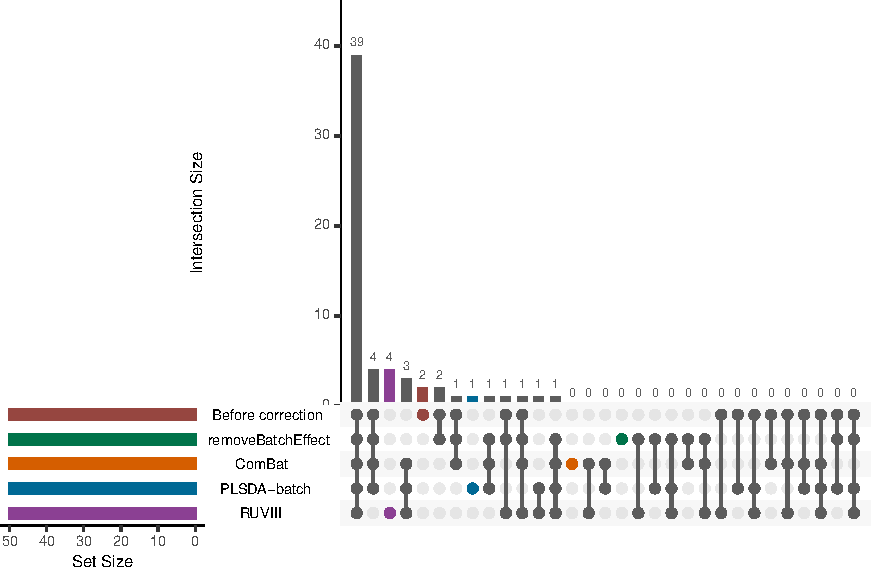
\includegraphics[width=1\linewidth]{PLSDAbatch_workflow_files/figure-latex/HFHSupsetR-1} 

}

\caption{UpSet plot showing overlap between variables selected from different corrected data for the HFHS study.}\label{fig:HFHSupsetR}
\end{figure}

In the above UpSet plot, the left bars indicate the number of variables selected from each data corrected with different methods. The right bar plot combined with the scatterplot show different intersection and their aggregates. We obtained an overlap of 39 out of 50 selected variables between different corrected and uncorrected data. However, the data from each method still included unique variables that were not selected in the other corrected data. As \texttt{upset()} can only include five datasets at once, we only display the uncorrected data and four corrected data that have been efficiently corrected for batch effects from our previous assessments.

\begin{Shaded}
\begin{Highlighting}[]
\NormalTok{hfhs.splsda.select.overlap }\OtherTok{\textless{}{-}} \FunctionTok{venn}\NormalTok{(hfhs.splsda.select, }\AttributeTok{show.plot =}\NormalTok{ F)}
\NormalTok{hfhs.inters.splsda }\OtherTok{\textless{}{-}} \FunctionTok{attr}\NormalTok{(hfhs.splsda.select.overlap, }\StringTok{\textquotesingle{}intersections\textquotesingle{}}\NormalTok{)}
\NormalTok{hfhs.inters.splsda.taxa }\OtherTok{\textless{}{-}} 
  \FunctionTok{lapply}\NormalTok{(hfhs.inters.splsda, }
         \AttributeTok{FUN =} \ControlFlowTok{function}\NormalTok{(x)\{}\FunctionTok{as.data.frame}\NormalTok{(HFHS\_data}\SpecialCharTok{$}\NormalTok{FullData}\SpecialCharTok{$}\NormalTok{taxa[x, ])\})}
\FunctionTok{capture.output}\NormalTok{(hfhs.inters.splsda.taxa, }
               \AttributeTok{file =} \StringTok{"GeneratedData/HFHSselected\_50\_splsda.txt"}\NormalTok{)}
\end{Highlighting}
\end{Shaded}

\hypertarget{hd-data}{%
\section{HD data}\label{hd-data}}

\hypertarget{data-pre-processing-3}{%
\subsection{Data pre-processing}\label{data-pre-processing-3}}

\hypertarget{prefiltering-1}{%
\subsubsection{Prefiltering}\label{prefiltering-1}}

We load the \textcolor{violet}{HD data} stored internally with function \texttt{data()}.

\begin{Shaded}
\begin{Highlighting}[]
\FunctionTok{data}\NormalTok{(}\StringTok{\textquotesingle{}HD\_data\textquotesingle{}}\NormalTok{) }
\NormalTok{hd.count }\OtherTok{\textless{}{-}}\NormalTok{ HD\_data}\SpecialCharTok{$}\NormalTok{FullData}\SpecialCharTok{$}\NormalTok{X.count}
\FunctionTok{dim}\NormalTok{(hd.count)}
\end{Highlighting}
\end{Shaded}

\begin{verbatim}
## [1]  30 368
\end{verbatim}

\begin{Shaded}
\begin{Highlighting}[]
\NormalTok{hd.filter.res }\OtherTok{\textless{}{-}} \FunctionTok{PreFL}\NormalTok{(}\AttributeTok{data =}\NormalTok{ hd.count)}
\NormalTok{hd.filter }\OtherTok{\textless{}{-}}\NormalTok{ hd.filter.res}\SpecialCharTok{$}\NormalTok{data.filter}
\FunctionTok{dim}\NormalTok{(hd.filter)}
\end{Highlighting}
\end{Shaded}

\begin{verbatim}
## [1]  30 269
\end{verbatim}

\begin{Shaded}
\begin{Highlighting}[]
\CommentTok{\# zero proportion before filtering}
\NormalTok{hd.filter.res}\SpecialCharTok{$}\NormalTok{zero.prob}
\end{Highlighting}
\end{Shaded}

\begin{verbatim}
## [1] 0.4509058
\end{verbatim}

\begin{Shaded}
\begin{Highlighting}[]
\CommentTok{\# zero proportion after filtering}
\FunctionTok{sum}\NormalTok{(hd.filter }\SpecialCharTok{==} \DecValTok{0}\NormalTok{)}\SpecialCharTok{/}\NormalTok{(}\FunctionTok{nrow}\NormalTok{(hd.filter) }\SpecialCharTok{*} \FunctionTok{ncol}\NormalTok{(hd.filter))}
\end{Highlighting}
\end{Shaded}

\begin{verbatim}
## [1] 0.3343247
\end{verbatim}

The raw \textcolor{violet}{HD data} include 368 OTUs and 30 samples. We use the function \texttt{PreFL()} from our \textcolor{orange}{PLSDAbatch} R package to filter the data. After filtering, the \textcolor{violet}{HD data} were reduced to 269 OTUs and 30 samples. The proportion of zeroes was reduced from 45\% to 33\%.

\hypertarget{transformation-3}{%
\subsubsection{Transformation}\label{transformation-3}}

Prior to CLR transformation, we add 1 as the offset for the \textcolor{violet}{HD data} - that are raw count data. We use \texttt{logratio.transfo()} function in \textcolor{orange}{mixOmics} package to CLR transform the data.

\begin{Shaded}
\begin{Highlighting}[]
\NormalTok{hd.clr }\OtherTok{\textless{}{-}} \FunctionTok{logratio.transfo}\NormalTok{(}\AttributeTok{X =}\NormalTok{ hd.filter, }\AttributeTok{logratio =} \StringTok{\textquotesingle{}CLR\textquotesingle{}}\NormalTok{, }\AttributeTok{offset =} \DecValTok{1}\NormalTok{)}

\FunctionTok{class}\NormalTok{(hd.clr) }\OtherTok{\textless{}{-}} \StringTok{\textquotesingle{}matrix\textquotesingle{}}
\end{Highlighting}
\end{Shaded}

\hypertarget{batch-effect-detection-3}{%
\subsection{Batch effect detection}\label{batch-effect-detection-3}}

\hypertarget{pca-3}{%
\subsubsection{PCA}\label{pca-3}}

We apply \texttt{pca()} function from \textcolor{orange}{mixOmics} package to the \textcolor{violet}{HD data} and use \texttt{Scatter\_Density()} function from \textcolor{orange}{PLSDAbatch} to represent the PCA sample plot with densities.

\begin{Shaded}
\begin{Highlighting}[]
\CommentTok{\# HD data}
\NormalTok{hd.pca.before }\OtherTok{\textless{}{-}} \FunctionTok{pca}\NormalTok{(hd.clr, }\AttributeTok{ncomp =} \DecValTok{3}\NormalTok{, }\AttributeTok{scale =} \ConstantTok{TRUE}\NormalTok{)}

\NormalTok{hd.metadata }\OtherTok{\textless{}{-}}\NormalTok{ HD\_data}\SpecialCharTok{$}\NormalTok{FullData}\SpecialCharTok{$}\NormalTok{metadata}

\NormalTok{hd.batch }\OtherTok{\textless{}{-}} \FunctionTok{as.factor}\NormalTok{(hd.metadata}\SpecialCharTok{$}\NormalTok{Cage)}
\NormalTok{hd.trt }\OtherTok{\textless{}{-}} \FunctionTok{as.factor}\NormalTok{(hd.metadata}\SpecialCharTok{$}\NormalTok{Genotype)}
\FunctionTok{names}\NormalTok{(hd.batch) }\OtherTok{=} \FunctionTok{names}\NormalTok{(hd.trt) }\OtherTok{=} \FunctionTok{rownames}\NormalTok{(hd.metadata) }

\FunctionTok{Scatter\_Density}\NormalTok{(}\AttributeTok{object =}\NormalTok{ hd.pca.before, }
                \AttributeTok{batch =}\NormalTok{ hd.batch, }
                \AttributeTok{trt =}\NormalTok{ hd.trt, }
                \AttributeTok{title =} \StringTok{\textquotesingle{}HD data\textquotesingle{}}\NormalTok{, }
                \AttributeTok{trt.legend.title =} \StringTok{\textquotesingle{}Genotype\textquotesingle{}}\NormalTok{, }
                \AttributeTok{batch.legend.title =} \StringTok{\textquotesingle{}Cage\textquotesingle{}}\NormalTok{, }\AttributeTok{legend.cex =} \FloatTok{0.6}\NormalTok{)}
\end{Highlighting}
\end{Shaded}

\begin{figure}

{\centering 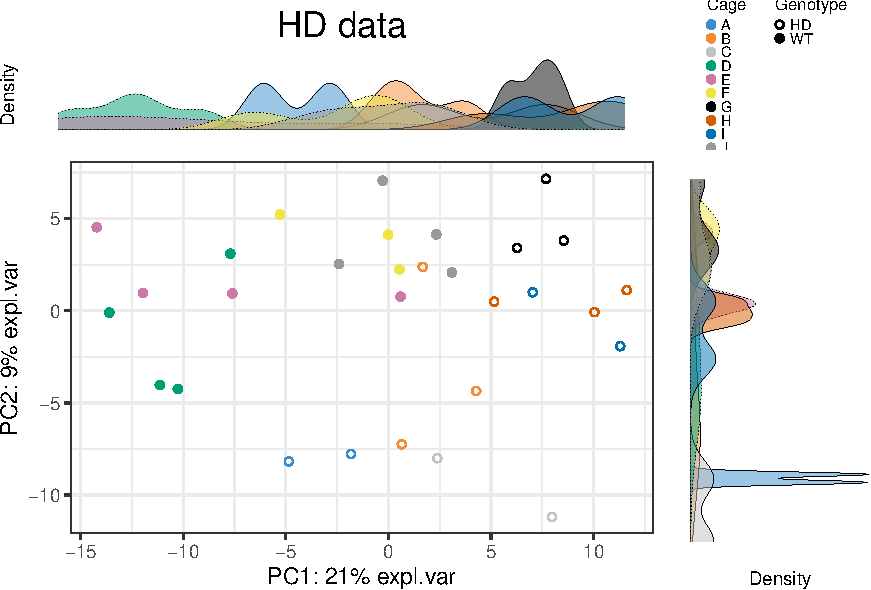
\includegraphics[width=0.6\linewidth]{PLSDAbatch_workflow_files/figure-latex/HDpcaBefore-1} 

}

\caption{The PCA sample plot with densities in the HD data.}\label{fig:HDpcaBefore}
\end{figure}

In the above figure, we observed a clear difference between genotypes but vague separation between cages on the PCA plot.

\hypertarget{heatmap-3}{%
\subsubsection{Heatmap}\label{heatmap-3}}

We produce a heatmap using \textcolor{orange}{pheatmap} package. The data first need to be scaled on both OTUs and samples.

\begin{Shaded}
\begin{Highlighting}[]
\CommentTok{\# scale the clr data on both OTUs and samples}
\NormalTok{hd.clr.s }\OtherTok{\textless{}{-}} \FunctionTok{scale}\NormalTok{(hd.clr, }\AttributeTok{center =}\NormalTok{ T, }\AttributeTok{scale =}\NormalTok{ T)}
\NormalTok{hd.clr.ss }\OtherTok{\textless{}{-}} \FunctionTok{scale}\NormalTok{(}\FunctionTok{t}\NormalTok{(hd.clr.s), }\AttributeTok{center =}\NormalTok{ T, }\AttributeTok{scale =}\NormalTok{ T)}

\NormalTok{hd.anno\_col }\OtherTok{\textless{}{-}} \FunctionTok{data.frame}\NormalTok{(}\AttributeTok{Cage =}\NormalTok{ hd.batch, }\AttributeTok{Genotype =}\NormalTok{ hd.trt)}
\NormalTok{hd.anno\_colors }\OtherTok{\textless{}{-}} \FunctionTok{list}\NormalTok{(}\AttributeTok{Cage =} \FunctionTok{color.mixo}\NormalTok{(}\DecValTok{1}\SpecialCharTok{:}\DecValTok{10}\NormalTok{), }
                       \AttributeTok{Genotype =} \FunctionTok{pb\_color}\NormalTok{(}\DecValTok{1}\SpecialCharTok{:}\DecValTok{2}\NormalTok{))}
\FunctionTok{names}\NormalTok{(hd.anno\_colors}\SpecialCharTok{$}\NormalTok{Cage) }\OtherTok{=} \FunctionTok{levels}\NormalTok{(hd.batch)}
\FunctionTok{names}\NormalTok{(hd.anno\_colors}\SpecialCharTok{$}\NormalTok{Genotype) }\OtherTok{=} \FunctionTok{levels}\NormalTok{(hd.trt)}

\FunctionTok{pheatmap}\NormalTok{(hd.clr.ss, }
         \AttributeTok{cluster\_rows =}\NormalTok{ F, }
         \AttributeTok{fontsize\_row =} \DecValTok{4}\NormalTok{, }
         \AttributeTok{fontsize\_col =} \DecValTok{6}\NormalTok{,}
         \AttributeTok{fontsize =} \DecValTok{8}\NormalTok{,}
         \AttributeTok{clustering\_distance\_rows =} \StringTok{\textquotesingle{}euclidean\textquotesingle{}}\NormalTok{,}
         \AttributeTok{clustering\_method =} \StringTok{\textquotesingle{}ward.D\textquotesingle{}}\NormalTok{,}
         \AttributeTok{treeheight\_row =} \DecValTok{30}\NormalTok{,}
         \AttributeTok{annotation\_col =}\NormalTok{ hd.anno\_col,}
         \AttributeTok{annotation\_colors =}\NormalTok{ hd.anno\_colors,}
         \AttributeTok{border\_color =} \StringTok{\textquotesingle{}NA\textquotesingle{}}\NormalTok{,}
         \AttributeTok{main =} \StringTok{\textquotesingle{}HD data {-} Scaled\textquotesingle{}}\NormalTok{)}
\end{Highlighting}
\end{Shaded}

\begin{figure}

{\centering 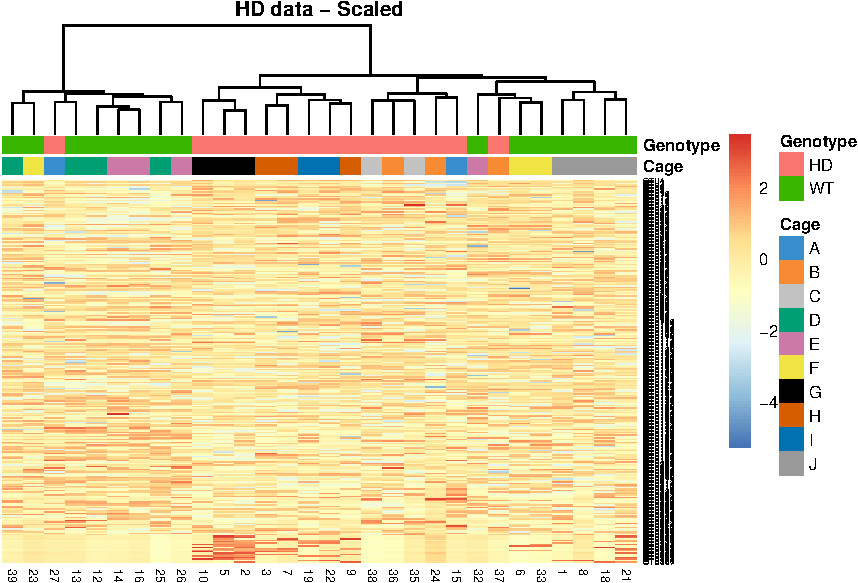
\includegraphics[width=0.9\linewidth]{PLSDAbatch_workflow_files/figure-latex/HDheatmap-1} 

}

\caption{Hierarchical clustering for samples in the HD data.}\label{fig:HDheatmap}
\end{figure}

In the heatmap, samples in the \textcolor{violet}{HD data} were mostly grouped by genotypes instead of cages, indicating a weak cage effect.

\hypertarget{prda-3}{%
\subsubsection{pRDA}\label{prda-3}}

We apply pRDA with \texttt{varpart()} function from \textcolor{orange}{vegan} R package.

\begin{Shaded}
\begin{Highlighting}[]
\NormalTok{hd.factors.df }\OtherTok{\textless{}{-}} \FunctionTok{data.frame}\NormalTok{(}\AttributeTok{trt =}\NormalTok{ hd.trt, }\AttributeTok{batch =}\NormalTok{ hd.batch)}
\NormalTok{hd.rda.before }\OtherTok{\textless{}{-}} \FunctionTok{varpart}\NormalTok{(hd.clr, }\SpecialCharTok{\textasciitilde{}}\NormalTok{ trt, }\SpecialCharTok{\textasciitilde{}}\NormalTok{ batch, }
                         \AttributeTok{data =}\NormalTok{ hd.factors.df, }\AttributeTok{scale =}\NormalTok{ T)}
\NormalTok{hd.rda.before}\SpecialCharTok{$}\NormalTok{part}\SpecialCharTok{$}\NormalTok{indfract}
\end{Highlighting}
\end{Shaded}

\begin{verbatim}
##                 Df R.squared Adj.R.squared Testable
## [a] = X1|X2      0        NA -2.220446e-16    FALSE
## [b] = X2|X1      8        NA  1.608205e-01     TRUE
## [c]              0        NA  9.730583e-02    FALSE
## [d] = Residuals NA        NA  7.418737e-01    FALSE
\end{verbatim}

In the result, \texttt{X1} and \texttt{X2} represent the first and second covariates fitted in the model. \texttt{{[}a{]}}, \texttt{{[}b{]}} represent the independent proportion of variance explained by \texttt{X1} and \texttt{X2} respectively, and \texttt{{[}c{]}} represents the intersection variance shared between \texttt{X1} and \texttt{X2}. Collinearity was detected in the \textcolor{violet}{HD data} between treatment and batch as indicated by lines \texttt{{[}a{]}} and \texttt{{[}c{]}} that all treatment variance (\texttt{{[}a{]}}: Adj.R.squared = 0, \texttt{{[}c{]}}: Adj.R.squared = 0.0973) was explained as intersection variance. The batch x treatment design in the \textcolor{violet}{HD data} is nested, in such a design the intersection variance is usually considerable. As the intersection is shared between batch and treatment effects, the batch variance in the \textcolor{violet}{HD data} is larger than the treatment variance.

\hypertarget{managing-batch-effects-3}{%
\subsection{Managing batch effects}\label{managing-batch-effects-3}}

Because of the nested batch x treatment design in the \textcolor{violet}{HD data}, the only way to account for the batch effect (i.e., the cage effect) is to apply linear mixed model and include the batch effect as a random effect.

\hypertarget{accounting-for-batch-effects-2}{%
\subsubsection{Accounting for batch effects}\label{accounting-for-batch-effects-2}}

\textbf{Linear regression}

Linear regression is conducted with \texttt{linear\_regres()} function in \textcolor{orange}{PLSDAbatch}. We integrated the \textcolor{orange}{performance} package that assesses performance of regression models into our function \texttt{linear\_regres()}. Therefore, we can apply \texttt{check\_model()} from \textcolor{orange}{performance} to the outputs from \texttt{linear\_regres()} to diagnose the validity of the model fitted with treatment and batch effects for each variable \citep{daniel2020performance}. We can extract performance measurements such as adjusted R2, RMSE, RSE, AIC and BIC for the models fitted with and without batch effects, which are also the outputs of \texttt{linear\_regres()}.

We apply a \texttt{linear\ mixed\ model} and fit the batch effect as a random effect because the design of the \textcolor{violet}{HD data} is nested. In such a design, the number of batches should be larger than treatment groups; otherwise, the linear mixed model cannot address the batch effect. Note: we assume that there is no interaction between batch and treatment effects on any microbial variable.

\begin{Shaded}
\begin{Highlighting}[]
\CommentTok{\# HD data}
\NormalTok{hd.clr }\OtherTok{\textless{}{-}}\NormalTok{ hd.clr[}\DecValTok{1}\SpecialCharTok{:}\FunctionTok{nrow}\NormalTok{(hd.clr), }\DecValTok{1}\SpecialCharTok{:}\FunctionTok{ncol}\NormalTok{(hd.clr)]}

\NormalTok{hd.lmm }\OtherTok{\textless{}{-}} \FunctionTok{linear\_regres}\NormalTok{(}\AttributeTok{data =}\NormalTok{ hd.clr, }\AttributeTok{trt =}\NormalTok{ hd.trt, }
                        \AttributeTok{batch.random =}\NormalTok{ hd.batch, }
                        \AttributeTok{type =} \StringTok{\textquotesingle{}linear mixed model\textquotesingle{}}\NormalTok{)}
\end{Highlighting}
\end{Shaded}

\begin{Shaded}
\begin{Highlighting}[]
\NormalTok{hd.p }\OtherTok{\textless{}{-}} \FunctionTok{sapply}\NormalTok{(hd.lmm}\SpecialCharTok{$}\NormalTok{lmm.table, }\ControlFlowTok{function}\NormalTok{(x)\{x}\SpecialCharTok{$}\NormalTok{coefficients[}\DecValTok{2}\NormalTok{,}\DecValTok{5}\NormalTok{]\})}
\NormalTok{hd.p.adj }\OtherTok{\textless{}{-}} \FunctionTok{p.adjust}\NormalTok{(}\AttributeTok{p =}\NormalTok{ hd.p, }\AttributeTok{method =} \StringTok{\textquotesingle{}fdr\textquotesingle{}}\NormalTok{)}

\FunctionTok{check\_model}\NormalTok{(hd.lmm}\SpecialCharTok{$}\NormalTok{model}\SpecialCharTok{$}\NormalTok{OTU1)}
\end{Highlighting}
\end{Shaded}

\begin{figure}

{\centering \includegraphics[width=1\linewidth]{PLSDAbatch_workflow_files/figure-latex/HDlmmS-1} 

}

\caption{Diagnostic plots for the model fitted with the cage effect of "OTU1" in the HD data.}\label{fig:HDlmmS}
\end{figure}

According to the diagnostic plots of ``OTU1'' as shown in the above figure panel, the simulated data under the fitted model were not very close to the real data (shown as green line), indicating an imperfect fitness (top panel). The linearity (or homoscedasticity) and homogeneity of variance were not satisfied. Some samples could be classified as outliers with a Cook's distance larger than or equal to 0.5, for example, ``12'', ``21'', ``20'', ``11'' and ``6'' (middle panel). The distribution of residuals was not normal, while the one of random effects was very close to normal (bottom panel).

We then look at the AIC of models fitted with or without batch effects.

\begin{Shaded}
\begin{Highlighting}[]
\FunctionTok{head}\NormalTok{(hd.lmm}\SpecialCharTok{$}\NormalTok{AIC)}
\end{Highlighting}
\end{Shaded}

\begin{verbatim}
##       trt.only trt.batch
## OTU1  60.00637  65.46410
## OTU2 130.14167 130.96344
## OTU3  71.76985  75.58915
## OTU4 134.59992 134.04812
## OTU5 150.25059 148.30644
## OTU6  99.92864  99.05391
\end{verbatim}

For some OTUs, the model fitted without batch effects is better with a lower AIC. For example, ``OTU1'' and ``OTU3''. ``OTU5'' is more appropriate within a model with batch effects. The others are similar within either model.

Since we apply a \texttt{"linear\ mixed\ model"} to the \textcolor{violet}{HD data}, this type of model can only output conditional \(R^2\) that includes the variance of both fixed and random effects (treatment, fixed and random batch effects) and marginal \(R^2\) that includes only the variance of fixed effects (treatment and fixed batch effects) \citep{nakagawa2013general}. The marginal \(R^2\)s of the models with and without the batch effect should be the same theoretically, as marginal \(R^2\) only includes fixed effects and the treatment effect is the only fixed effect here. In the actual calculation, the results of these two models were not the same due to different ways of model fitting.

\begin{Shaded}
\begin{Highlighting}[]
\FunctionTok{head}\NormalTok{(hd.lmm}\SpecialCharTok{$}\NormalTok{cond.R2)}
\end{Highlighting}
\end{Shaded}

\begin{verbatim}
##        trt.only trt.batch
## OTU1 0.47917775 0.5161317
## OTU2 0.39223824 0.4729848
## OTU3 0.02091376 0.2636432
## OTU4 0.37200835 0.5672392
## OTU5 0.07858373 0.2938212
## OTU6 0.41388250 0.6143134
\end{verbatim}

\begin{Shaded}
\begin{Highlighting}[]
\FunctionTok{head}\NormalTok{(hd.lmm}\SpecialCharTok{$}\NormalTok{marg.R2)}
\end{Highlighting}
\end{Shaded}

\begin{verbatim}
##        trt.only  trt.batch
## OTU1 0.47917775 0.46735273
## OTU2 0.39223824 0.38459672
## OTU3 0.02091376 0.01489608
## OTU4 0.37200835 0.36122754
## OTU5 0.07858373 0.06052938
## OTU6 0.41388250 0.40749149
\end{verbatim}

We observed that some variables resulted in singular fits (\texttt{error\ message:\ Can\textquotesingle{}t\ compute\ random\ effect\ variances.\ Some\ variance\ components\ equal\ zero.\ Your\ model\ may\ suffer\ from\ singulariy.}), which are expected to happen in linear mixed models when covariates are nested. We recommend noting the variables for which this error occurs, as it may lead to unreliable results.

\hypertarget{references-1}{%
\section{References}\label{references-1}}

\hypertarget{batch-effects-management-in-simulation-studies-gaussian-distribution}{%
\chapter{Batch Effects Management in Simulation Studies (Gaussian Distribution)}\label{batch-effects-management-in-simulation-studies-gaussian-distribution}}

\hypertarget{introduction-1}{%
\section{Introduction}\label{introduction-1}}

We adapted the simulation strategy that is component-based and multivariate from \citep{singh2019diablo}. We assumed the input data after filtering follow a lognormal distribution inspired from \citep{weiss2017normalization}, thus after Centered Log Ratio (CLR) transformed follow a Gaussian distribution. Thus, we simulated components from a Gaussian distribution across all samples. The data matrix was generated based on the simulated components and corresponding loading vectors for each variable. Each simulated dataset included 300 variables and 40 samples grouped according to two treatments (trt1 and trt2) and two batches (batch1 and batch2). Different parameters including amount of batch and treatment variability among samples, number of variables with batch and/or treatment effects, balanced and unbalanced batch \(\times\) treatment designs were considered and summarised in the table below.

\textbf{Table 1: Summary of simulation scenarios (Gaussian distribution).} For a given choice of parameters reported in this table, each simulation was repeated 50 times. \(M^{(trt)}, M^{(batch)}\) and \(M^{(trt \ \& \ batch)}\) represent the number of variables with treatment, batch, or both effects respectively. \textbf{Simu 6} includes parameters reflective of real data.

\begin{longtable}[]{@{}
  >{\centering\arraybackslash}p{(\columnwidth - 14\tabcolsep) * \real{0.0833}}
  >{\centering\arraybackslash}p{(\columnwidth - 14\tabcolsep) * \real{0.1042}}
  >{\centering\arraybackslash}p{(\columnwidth - 14\tabcolsep) * \real{0.1319}}
  >{\centering\arraybackslash}p{(\columnwidth - 14\tabcolsep) * \real{0.1181}}
  >{\centering\arraybackslash}p{(\columnwidth - 14\tabcolsep) * \real{0.1458}}
  >{\centering\arraybackslash}p{(\columnwidth - 14\tabcolsep) * \real{0.1181}}
  >{\centering\arraybackslash}p{(\columnwidth - 14\tabcolsep) * \real{0.1181}}
  >{\centering\arraybackslash}p{(\columnwidth - 14\tabcolsep) * \real{0.1806}}@{}}
\toprule()
\begin{minipage}[b]{\linewidth}\centering
\end{minipage} & \begin{minipage}[b]{\linewidth}\centering
\(\mu_{(trt)}\)
\end{minipage} & \begin{minipage}[b]{\linewidth}\centering
\(\sigma'_{(trt)}\)
\end{minipage} & \begin{minipage}[b]{\linewidth}\centering
\(\mu_{(batch)}\)
\end{minipage} & \begin{minipage}[b]{\linewidth}\centering
\(\sigma'_{(batch)}\)
\end{minipage} & \begin{minipage}[b]{\linewidth}\centering
\(M^{(trt)}\)
\end{minipage} & \begin{minipage}[b]{\linewidth}\centering
\(M^{(batch)}\)
\end{minipage} & \begin{minipage}[b]{\linewidth}\centering
\(M^{(trt \ \& \ batch)}\)
\end{minipage} \\
\midrule()
\endhead
Simu 1 & 3 & 1 & 7 & \{1,4,8\} & 60 & 150 & 0 \\
Simu 2 & \{3,5,7\} & 1 & 7 & 8 & 60 & 150 & 0 \\
Simu 3 & 3 & \{1,2,4\} & 7 & 8 & 60 & 150 & 0 \\
Simu 4 & 3 & 2 & 7 & 8 & \{30,60,100,150\} & 150 & 0 \\
Simu 5 & 3 & 2 & 7 & 8 & 60 & \{30,60,100,150\} & 0 \\
\textbf{Simu 6} & 3 & 2 & 7 & 8 & 60 & 150 & \{0,18,30,42,60\} \\
\bottomrule()
\end{longtable}

We first generated two base components \(t^{(trt)}\) and \(t^{(batch)}\) to represent the underlying treatment and batch variation across samples in the datasets. The samples with trt1 or trt2 in the component \(t^{(trt)}\) were generated from \(N(-\mu_{(trt)}, \sigma^{'2}_{(trt)})\) and \(N(\mu_{(trt)}, \sigma^{'2}_{(trt)})\) respectively, where \(\sigma^{'2}_{(trt)}\) refers to the variability of treatment effect among samples, and similarly for the batch component. We then sampled the corresponding loading vectors \(\alpha^{(trt)}\) and \(\alpha^{(batch)}\) from a uniform distribution \([-0.3, -0.2]\cup [0.2,0.3]\) respectively and scaled them as an unit vector. We subsequently constructed the treatment relevant matrix as \(X^{(trt)} = t^{(trt)}(\alpha^{(trt)})^{\top}\) and similarly for the batch relevant matrix.

We also generated background noise \(E\) (\(E \in \mathbb{R}^{40 \times 300}\)), where each element was randomly sampled from \(N(0, 0.2^{2})\). The final simulated dataset \(X_{result}\) was constructed based on the treatment, batch relevant matrices and background noise. Starting with \(X_{result} = E\), we then added different types of variables, such that:

\small

\[X_{result}[ ,\mbox{variables}^{(trt)}] = E[ ,\mbox{variables}^{(trt)}] + X^{(trt)}\]
\[X_{result}[ ,\mbox{variables}^{(batch)}] = X_{result}[ ,\mbox{variables}^{(batch)}] + X^{(batch)},\] \normalsize

\noindent where variables with treatment or batch effects were randomly indexed in the data.

In addition to the data with batch effects, we also simulated a ground-truth dataset that only included the background noise and treatment but no batch effect to evaluate batch effect corrected datasets.

In these simulation scenarios, for PLSDA-batch we set \(C-1\) (or \(B-1\)) components associated with treatment (or batch) effects (where \(C\) and \(B\) represent the total number of treatment and batch groups respectively) as \(C-1\) (\(B-1\)) components are likely to explain 100\% variance in \(Y\). The number of variables with a true treatment effect (\(M^{(trt)}\)) is set as the optimal number to select on each treatment component in sPLSDA-batch.

To save space, here we only describe one scenario that we believe is a representative of real data (\(M^{(trt \ \& \ batch)} = 30\), simu 6 in Table 1).

\hypertarget{simulations}{%
\section{Simulations}\label{simulations}}

\hypertarget{balanced-batch-times-treatment-design}{%
\subsection{\texorpdfstring{Balanced batch \(\times\) treatment design}{Balanced batch \textbackslash times treatment design}}\label{balanced-batch-times-treatment-design}}

The balanced batch \(\times\) treatment experimental design included 10 samples from two batches respectively in each treatment group (see Table 2)

\textbf{Table 2: Balanced batch \(\times\) treatment design} in the simulation study

\begin{longtable}[]{@{}ccc@{}}
\toprule()
& Trt1 & Trt2 \\
\midrule()
\endhead
Batch1 & 10 & 10 \\
Batch2 & 10 & 10 \\
\bottomrule()
\end{longtable}

\begin{Shaded}
\begin{Highlighting}[]
\NormalTok{nitr }\OtherTok{\textless{}{-}} \DecValTok{50}
\NormalTok{p\_total }\OtherTok{\textless{}{-}} \DecValTok{300}
\NormalTok{p\_trt\_relevant }\OtherTok{\textless{}{-}} \DecValTok{60}
\NormalTok{p\_bat\_relevant }\OtherTok{\textless{}{-}} \DecValTok{150}

\CommentTok{\# global variance (RDA)}
\NormalTok{gvar.before }\OtherTok{\textless{}{-}}\NormalTok{ gvar.clean }\OtherTok{\textless{}{-}}\NormalTok{ gvar.rbe }\OtherTok{\textless{}{-}}\NormalTok{ gvar.combat }\OtherTok{\textless{}{-}} 
\NormalTok{  gvar.plsdab }\OtherTok{\textless{}{-}}\NormalTok{ gvar.splsdab }\OtherTok{\textless{}{-}} \FunctionTok{data.frame}\NormalTok{(}\AttributeTok{treatment =} \ConstantTok{NA}\NormalTok{, }\AttributeTok{batch =} \ConstantTok{NA}\NormalTok{,  }
                                            \AttributeTok{intersection =} \ConstantTok{NA}\NormalTok{, }
                                            \AttributeTok{residual =} \ConstantTok{NA}\NormalTok{)}

\CommentTok{\# individual variance (R2)}
\NormalTok{r2.trt.before }\OtherTok{\textless{}{-}}\NormalTok{ r2.trt.clean }\OtherTok{\textless{}{-}}\NormalTok{ r2.trt.rbe  }\OtherTok{\textless{}{-}}\NormalTok{ r2.trt.combat }\OtherTok{\textless{}{-}} 
\NormalTok{  r2.trt.plsdab }\OtherTok{\textless{}{-}}\NormalTok{ r2.trt.splsdab }\OtherTok{\textless{}{-}} \FunctionTok{data.frame}\NormalTok{(}\FunctionTok{matrix}\NormalTok{(}\ConstantTok{NA}\NormalTok{, }\AttributeTok{nrow =}\NormalTok{ p\_total, }
                                                       \AttributeTok{ncol =}\NormalTok{ nitr))}
\NormalTok{r2.batch.before }\OtherTok{\textless{}{-}}\NormalTok{ r2.batch.clean }\OtherTok{\textless{}{-}}\NormalTok{ r2.batch.rbe  }\OtherTok{\textless{}{-}}\NormalTok{ r2.batch.combat }\OtherTok{\textless{}{-}} 
\NormalTok{  r2.batch.plsdab }\OtherTok{\textless{}{-}}\NormalTok{ r2.batch.splsdab }\OtherTok{\textless{}{-}} \FunctionTok{data.frame}\NormalTok{(}\FunctionTok{matrix}\NormalTok{(}\ConstantTok{NA}\NormalTok{, }\AttributeTok{nrow =}\NormalTok{ p\_total, }
                                                           \AttributeTok{ncol =}\NormalTok{ nitr))}

\CommentTok{\# precision \& recall \& F1 (ANOVA)}
\NormalTok{precision\_limma }\OtherTok{\textless{}{-}}\NormalTok{ recall\_limma }\OtherTok{\textless{}{-}}\NormalTok{ F1\_limma }\OtherTok{\textless{}{-}} 
  \FunctionTok{data.frame}\NormalTok{(}\AttributeTok{before =} \ConstantTok{NA}\NormalTok{, }\AttributeTok{clean =} \ConstantTok{NA}\NormalTok{, }\AttributeTok{rbe =} \ConstantTok{NA}\NormalTok{, }\AttributeTok{combat =} \ConstantTok{NA}\NormalTok{, }
             \AttributeTok{plsda\_batch =} \ConstantTok{NA}\NormalTok{, }\AttributeTok{splsda\_batch =} \ConstantTok{NA}\NormalTok{)}

\CommentTok{\# precision \& recall \& F1 (sPLSDA)}
\NormalTok{precision\_splsda }\OtherTok{\textless{}{-}}\NormalTok{ recall\_splsda }\OtherTok{\textless{}{-}}\NormalTok{ F1\_splsda }\OtherTok{\textless{}{-}} 
  \FunctionTok{data.frame}\NormalTok{(}\AttributeTok{before =} \ConstantTok{NA}\NormalTok{, }\AttributeTok{clean =} \ConstantTok{NA}\NormalTok{, }\AttributeTok{rbe =} \ConstantTok{NA}\NormalTok{, }\AttributeTok{combat =} \ConstantTok{NA}\NormalTok{, }
             \AttributeTok{plsda\_batch =} \ConstantTok{NA}\NormalTok{, }\AttributeTok{splsda\_batch =} \ConstantTok{NA}\NormalTok{)}

\ControlFlowTok{for}\NormalTok{(i }\ControlFlowTok{in} \FunctionTok{seq\_len}\NormalTok{(nitr))\{}
  \DocumentationTok{\#\#\# initial setup }\AlertTok{\#\#\#}
\NormalTok{  simulation }\OtherTok{\textless{}{-}} \FunctionTok{simData\_Gaussian}\NormalTok{(}\AttributeTok{mean.batch =} \DecValTok{7}\NormalTok{, }\AttributeTok{sd.batch =} \DecValTok{8}\NormalTok{, }
                                 \AttributeTok{mean.trt =} \DecValTok{3}\NormalTok{, }\AttributeTok{sd.trt =} \DecValTok{2}\NormalTok{, }
                                 \AttributeTok{N =} \DecValTok{40}\NormalTok{, }\AttributeTok{p\_total =} \DecValTok{300}\NormalTok{, }
                                 \AttributeTok{p\_trt\_relevant =} \DecValTok{60}\NormalTok{, }
                                 \AttributeTok{p\_bat\_relevant =} \DecValTok{150}\NormalTok{, }
                                 \AttributeTok{percentage\_overlap\_samples =} \FloatTok{0.5}\NormalTok{,}
                                 \AttributeTok{percentage\_overlap\_variables =} \FloatTok{0.5}\NormalTok{, }\AttributeTok{seeds =}\NormalTok{ i)}
  
\NormalTok{  X }\OtherTok{\textless{}{-}}\NormalTok{ simulation}\SpecialCharTok{$}\NormalTok{data}
\NormalTok{  trt }\OtherTok{\textless{}{-}}\NormalTok{ simulation}\SpecialCharTok{$}\NormalTok{Y.trt}
\NormalTok{  batch }\OtherTok{\textless{}{-}}\NormalTok{ simulation}\SpecialCharTok{$}\NormalTok{Y.bat}
\NormalTok{  true.trt }\OtherTok{\textless{}{-}}\NormalTok{ simulation}\SpecialCharTok{$}\NormalTok{true.trt}
\NormalTok{  true.batch }\OtherTok{\textless{}{-}}\NormalTok{ simulation}\SpecialCharTok{$}\NormalTok{true.batch}
  
\NormalTok{  Batch\_Trt.factors }\OtherTok{\textless{}{-}} \FunctionTok{data.frame}\NormalTok{(}\AttributeTok{Batch =}\NormalTok{ batch, }\AttributeTok{Treatment =}\NormalTok{ trt)}
  
  \DocumentationTok{\#\#\# Before correction }\AlertTok{\#\#\#}
  \CommentTok{\# global variance (RDA)}
\NormalTok{  rda.before }\OtherTok{=} \FunctionTok{varpart}\NormalTok{(}\FunctionTok{scale}\NormalTok{(X), }\SpecialCharTok{\textasciitilde{}}\NormalTok{ Treatment, }\SpecialCharTok{\textasciitilde{}}\NormalTok{ Batch, }
                       \AttributeTok{data =}\NormalTok{ Batch\_Trt.factors)}
\NormalTok{  gvar.before[i, ] }\OtherTok{\textless{}{-}}\NormalTok{ rda.before}\SpecialCharTok{$}\NormalTok{part}\SpecialCharTok{$}\NormalTok{indfract}\SpecialCharTok{$}\NormalTok{Adj.R.squared}
  
  \CommentTok{\# individual variance (R2)}
\NormalTok{  indiv.trt.before }\OtherTok{\textless{}{-}} \FunctionTok{c}\NormalTok{()}
\NormalTok{  indiv.batch.before }\OtherTok{\textless{}{-}} \FunctionTok{c}\NormalTok{()}
  \ControlFlowTok{for}\NormalTok{(c }\ControlFlowTok{in} \FunctionTok{seq\_len}\NormalTok{(}\FunctionTok{ncol}\NormalTok{(X)))\{}
\NormalTok{    fit.res1 }\OtherTok{\textless{}{-}} \FunctionTok{lm}\NormalTok{(}\FunctionTok{scale}\NormalTok{(X)[ ,c] }\SpecialCharTok{\textasciitilde{}}\NormalTok{ trt)}
\NormalTok{    fit.summary1 }\OtherTok{\textless{}{-}} \FunctionTok{summary}\NormalTok{(fit.res1)}
\NormalTok{    fit.res2 }\OtherTok{\textless{}{-}} \FunctionTok{lm}\NormalTok{(}\FunctionTok{scale}\NormalTok{(X)[ ,c] }\SpecialCharTok{\textasciitilde{}}\NormalTok{ batch)}
\NormalTok{    fit.summary2 }\OtherTok{\textless{}{-}} \FunctionTok{summary}\NormalTok{(fit.res2)}
\NormalTok{    indiv.trt.before }\OtherTok{\textless{}{-}} \FunctionTok{c}\NormalTok{(indiv.trt.before, fit.summary1}\SpecialCharTok{$}\NormalTok{r.squared)}
\NormalTok{    indiv.batch.before }\OtherTok{\textless{}{-}} \FunctionTok{c}\NormalTok{(indiv.batch.before, fit.summary2}\SpecialCharTok{$}\NormalTok{r.squared)}
\NormalTok{  \}}
\NormalTok{  r2.trt.before[ ,i] }\OtherTok{\textless{}{-}}\NormalTok{  indiv.trt.before}
\NormalTok{  r2.batch.before[ ,i] }\OtherTok{\textless{}{-}}\NormalTok{  indiv.batch.before}
  
  \CommentTok{\# precision \& recall \& F1 (ANOVA)}
\NormalTok{  fit.before }\OtherTok{\textless{}{-}} \FunctionTok{lmFit}\NormalTok{(}\FunctionTok{t}\NormalTok{(}\FunctionTok{scale}\NormalTok{(X)), }\AttributeTok{design =} \FunctionTok{model.matrix}\NormalTok{( }\SpecialCharTok{\textasciitilde{}} \DecValTok{0} \SpecialCharTok{+} \FunctionTok{as.factor}\NormalTok{(trt)))}
\NormalTok{  fit.before }\OtherTok{\textless{}{-}} \FunctionTok{contrasts.fit}\NormalTok{(fit.before, }\AttributeTok{contrasts =} \FunctionTok{c}\NormalTok{(}\DecValTok{1}\NormalTok{,}\SpecialCharTok{{-}}\DecValTok{1}\NormalTok{))}
\NormalTok{  fit.result.before }\OtherTok{\textless{}{-}} \FunctionTok{topTable}\NormalTok{(}\FunctionTok{eBayes}\NormalTok{(fit.before), }\AttributeTok{number =}\NormalTok{ p\_total)}
\NormalTok{  otu.sig.before }\OtherTok{\textless{}{-}} \FunctionTok{rownames}\NormalTok{(fit.result.before)[fit.result.before}\SpecialCharTok{$}\NormalTok{adj.P.Val }\SpecialCharTok{\textless{}=} 
                                                  \FloatTok{0.05}\NormalTok{]}
  
\NormalTok{  precision\_limma.before }\OtherTok{\textless{}{-}} \FunctionTok{length}\NormalTok{(}\FunctionTok{intersect}\NormalTok{(true.trt, otu.sig.before))}\SpecialCharTok{/}
    \FunctionTok{length}\NormalTok{(otu.sig.before)}
\NormalTok{  recall\_limma.before }\OtherTok{\textless{}{-}} \FunctionTok{length}\NormalTok{(}\FunctionTok{intersect}\NormalTok{(true.trt, otu.sig.before))}\SpecialCharTok{/}
    \FunctionTok{length}\NormalTok{(true.trt)}
\NormalTok{  F1\_limma.before }\OtherTok{\textless{}{-}}\NormalTok{ (}\DecValTok{2}\SpecialCharTok{*}\NormalTok{precision\_limma.before}\SpecialCharTok{*}\NormalTok{recall\_limma.before)}\SpecialCharTok{/}
\NormalTok{    (precision\_limma.before }\SpecialCharTok{+}\NormalTok{ recall\_limma.before)}
  
  \DocumentationTok{\#\# replace NA value with 0}
  \ControlFlowTok{if}\NormalTok{(precision\_limma.before }\SpecialCharTok{==} \StringTok{\textquotesingle{}NaN\textquotesingle{}}\NormalTok{)\{}
\NormalTok{    precision\_limma.before }\OtherTok{=} \DecValTok{0}
\NormalTok{  \}}
  \ControlFlowTok{if}\NormalTok{(F1\_limma.before }\SpecialCharTok{==} \StringTok{\textquotesingle{}NaN\textquotesingle{}}\NormalTok{)\{}
\NormalTok{    F1\_limma.before }\OtherTok{=} \DecValTok{0}
\NormalTok{  \}}
  
  \CommentTok{\# precision \& recall \& F1 (sPLSDA)}
\NormalTok{  fit.before\_splsda }\OtherTok{\textless{}{-}} \FunctionTok{splsda}\NormalTok{(}\AttributeTok{X =}\NormalTok{ X, }\AttributeTok{Y =}\NormalTok{ trt, }\AttributeTok{ncomp =} \DecValTok{1}\NormalTok{, }
                              \AttributeTok{keepX =} \FunctionTok{length}\NormalTok{(true.trt))}
\NormalTok{  otu.dcn.before }\OtherTok{\textless{}{-}} \FunctionTok{which}\NormalTok{(fit.before\_splsda}\SpecialCharTok{$}\NormalTok{loadings}\SpecialCharTok{$}\NormalTok{X[ ,}\DecValTok{1}\NormalTok{] }\SpecialCharTok{!=} \DecValTok{0}\NormalTok{)}
  
\NormalTok{  precision\_splsda.before }\OtherTok{\textless{}{-}} \FunctionTok{length}\NormalTok{(}\FunctionTok{intersect}\NormalTok{(true.trt, otu.dcn.before))}\SpecialCharTok{/}
    \FunctionTok{length}\NormalTok{(otu.dcn.before)}
\NormalTok{  recall\_splsda.before }\OtherTok{\textless{}{-}} \FunctionTok{length}\NormalTok{(}\FunctionTok{intersect}\NormalTok{(true.trt, otu.dcn.before))}\SpecialCharTok{/}
    \FunctionTok{length}\NormalTok{(true.trt)}
\NormalTok{  F1\_splsda.before }\OtherTok{\textless{}{-}}\NormalTok{ (}\DecValTok{2}\SpecialCharTok{*}\NormalTok{precision\_splsda.before}\SpecialCharTok{*}\NormalTok{recall\_splsda.before)}\SpecialCharTok{/}
\NormalTok{    (precision\_splsda.before }\SpecialCharTok{+}\NormalTok{ recall\_splsda.before)}
  
  \DocumentationTok{\#\# replace NA value with 0}
  \ControlFlowTok{if}\NormalTok{(F1\_splsda.before }\SpecialCharTok{==} \StringTok{\textquotesingle{}NaN\textquotesingle{}}\NormalTok{)\{}
\NormalTok{    F1\_splsda.before }\OtherTok{=} \DecValTok{0}
\NormalTok{  \}}
  
  \DocumentationTok{\#\#\#\#\#\#\#\#\#\#\#\#\#\#\#\#\#\#\#\#\#\#\#\#\#\#\#\#\#\#\#\#\#\#\#\#\#\#\#\#\#\#\#\#\#\#\#\#\#\#\#\#\#\#\#\#\#\#\#\#\#\#\#\#\#\#\#\#\#\#\#\#\#\#\#\#\#\#}
  \DocumentationTok{\#\#\# Ground{-}truth data }\AlertTok{\#\#\#}
\NormalTok{  X.clean }\OtherTok{\textless{}{-}}\NormalTok{ simulation}\SpecialCharTok{$}\NormalTok{cleanData}
  \CommentTok{\# global variance (RDA)}
\NormalTok{  rda.clean }\OtherTok{=} \FunctionTok{varpart}\NormalTok{(}\FunctionTok{scale}\NormalTok{(X.clean), }\SpecialCharTok{\textasciitilde{}}\NormalTok{ Treatment, }\SpecialCharTok{\textasciitilde{}}\NormalTok{ Batch, }
                      \AttributeTok{data =}\NormalTok{ Batch\_Trt.factors)}
\NormalTok{  gvar.clean[i, ] }\OtherTok{\textless{}{-}}\NormalTok{ rda.clean}\SpecialCharTok{$}\NormalTok{part}\SpecialCharTok{$}\NormalTok{indfract}\SpecialCharTok{$}\NormalTok{Adj.R.squared}
  
  \CommentTok{\# individual variance (R2)}
\NormalTok{  indiv.trt.clean }\OtherTok{\textless{}{-}} \FunctionTok{c}\NormalTok{()}
\NormalTok{  indiv.batch.clean }\OtherTok{\textless{}{-}} \FunctionTok{c}\NormalTok{()}
  \ControlFlowTok{for}\NormalTok{(c }\ControlFlowTok{in} \FunctionTok{seq\_len}\NormalTok{(}\FunctionTok{ncol}\NormalTok{(X.clean)))\{}
\NormalTok{    fit.res1 }\OtherTok{\textless{}{-}} \FunctionTok{lm}\NormalTok{(}\FunctionTok{scale}\NormalTok{(X.clean)[ ,c] }\SpecialCharTok{\textasciitilde{}}\NormalTok{ trt)}
\NormalTok{    fit.summary1 }\OtherTok{\textless{}{-}} \FunctionTok{summary}\NormalTok{(fit.res1)}
\NormalTok{    fit.res2 }\OtherTok{\textless{}{-}} \FunctionTok{lm}\NormalTok{(}\FunctionTok{scale}\NormalTok{(X.clean)[ ,c] }\SpecialCharTok{\textasciitilde{}}\NormalTok{ batch)}
\NormalTok{    fit.summary2 }\OtherTok{\textless{}{-}} \FunctionTok{summary}\NormalTok{(fit.res2)}
\NormalTok{    indiv.trt.clean }\OtherTok{\textless{}{-}} \FunctionTok{c}\NormalTok{(indiv.trt.clean, fit.summary1}\SpecialCharTok{$}\NormalTok{r.squared)}
\NormalTok{    indiv.batch.clean }\OtherTok{\textless{}{-}} \FunctionTok{c}\NormalTok{(indiv.batch.clean, fit.summary2}\SpecialCharTok{$}\NormalTok{r.squared)}
\NormalTok{  \}}
\NormalTok{  r2.trt.clean[ ,i] }\OtherTok{\textless{}{-}}\NormalTok{  indiv.trt.clean}
\NormalTok{  r2.batch.clean[ ,i] }\OtherTok{\textless{}{-}}\NormalTok{  indiv.batch.clean}
  
  \CommentTok{\# precision \& recall \& F1 (ANOVA)}
\NormalTok{  fit.clean }\OtherTok{\textless{}{-}} \FunctionTok{lmFit}\NormalTok{(}\FunctionTok{t}\NormalTok{(}\FunctionTok{scale}\NormalTok{(X.clean)), }
                     \AttributeTok{design =} \FunctionTok{model.matrix}\NormalTok{( }\SpecialCharTok{\textasciitilde{}} \DecValTok{0} \SpecialCharTok{+} \FunctionTok{as.factor}\NormalTok{(trt)))}
\NormalTok{  fit.clean }\OtherTok{\textless{}{-}} \FunctionTok{contrasts.fit}\NormalTok{(fit.clean, }\AttributeTok{contrasts =} \FunctionTok{c}\NormalTok{(}\DecValTok{1}\NormalTok{,}\SpecialCharTok{{-}}\DecValTok{1}\NormalTok{))}
\NormalTok{  fit.result.clean }\OtherTok{\textless{}{-}} \FunctionTok{topTable}\NormalTok{(}\FunctionTok{eBayes}\NormalTok{(fit.clean), }\AttributeTok{number =}\NormalTok{ p\_total)}
\NormalTok{  otu.sig.clean }\OtherTok{\textless{}{-}} \FunctionTok{rownames}\NormalTok{(fit.result.clean)[fit.result.clean}\SpecialCharTok{$}\NormalTok{adj.P.Val }\SpecialCharTok{\textless{}=} 
                                                \FloatTok{0.05}\NormalTok{]}
  
\NormalTok{  precision\_limma.clean }\OtherTok{\textless{}{-}} \FunctionTok{length}\NormalTok{(}\FunctionTok{intersect}\NormalTok{(true.trt, otu.sig.clean))}\SpecialCharTok{/}
    \FunctionTok{length}\NormalTok{(otu.sig.clean)}
\NormalTok{  recall\_limma.clean }\OtherTok{\textless{}{-}} \FunctionTok{length}\NormalTok{(}\FunctionTok{intersect}\NormalTok{(true.trt, otu.sig.clean))}\SpecialCharTok{/}
    \FunctionTok{length}\NormalTok{(true.trt)}
\NormalTok{  F1\_limma.clean }\OtherTok{\textless{}{-}}\NormalTok{ (}\DecValTok{2}\SpecialCharTok{*}\NormalTok{precision\_limma.clean}\SpecialCharTok{*}\NormalTok{recall\_limma.clean)}\SpecialCharTok{/}
\NormalTok{    (precision\_limma.clean }\SpecialCharTok{+}\NormalTok{ recall\_limma.clean)}
  
  \DocumentationTok{\#\# replace NA value with 0}
  \ControlFlowTok{if}\NormalTok{(precision\_limma.clean }\SpecialCharTok{==} \StringTok{\textquotesingle{}NaN\textquotesingle{}}\NormalTok{)\{}
\NormalTok{    precision\_limma.clean }\OtherTok{=} \DecValTok{0}
\NormalTok{  \}}
  \ControlFlowTok{if}\NormalTok{(F1\_limma.clean }\SpecialCharTok{==} \StringTok{\textquotesingle{}NaN\textquotesingle{}}\NormalTok{)\{}
\NormalTok{    F1\_limma.clean }\OtherTok{=} \DecValTok{0}
\NormalTok{  \}}
  
  \CommentTok{\# precision \& recall \& F1 (sPLSDA)}
\NormalTok{  fit.clean\_splsda }\OtherTok{\textless{}{-}} \FunctionTok{splsda}\NormalTok{(}\AttributeTok{X =}\NormalTok{ X.clean, }\AttributeTok{Y =}\NormalTok{ trt, }\AttributeTok{ncomp =} \DecValTok{1}\NormalTok{, }
                             \AttributeTok{keepX =} \FunctionTok{length}\NormalTok{(true.trt))}
\NormalTok{  otu.dcn.clean }\OtherTok{\textless{}{-}} \FunctionTok{which}\NormalTok{(fit.clean\_splsda}\SpecialCharTok{$}\NormalTok{loadings}\SpecialCharTok{$}\NormalTok{X[ ,}\DecValTok{1}\NormalTok{] }\SpecialCharTok{!=} \DecValTok{0}\NormalTok{)}
  
\NormalTok{  precision\_splsda.clean }\OtherTok{\textless{}{-}} \FunctionTok{length}\NormalTok{(}\FunctionTok{intersect}\NormalTok{(true.trt, otu.dcn.clean))}\SpecialCharTok{/}
    \FunctionTok{length}\NormalTok{(otu.dcn.clean)}
\NormalTok{  recall\_splsda.clean }\OtherTok{\textless{}{-}} \FunctionTok{length}\NormalTok{(}\FunctionTok{intersect}\NormalTok{(true.trt, otu.dcn.clean))}\SpecialCharTok{/}
    \FunctionTok{length}\NormalTok{(true.trt)}
\NormalTok{  F1\_splsda.clean }\OtherTok{\textless{}{-}}\NormalTok{ (}\DecValTok{2}\SpecialCharTok{*}\NormalTok{precision\_splsda.clean}\SpecialCharTok{*}\NormalTok{recall\_splsda.clean)}\SpecialCharTok{/}
\NormalTok{    (precision\_splsda.clean }\SpecialCharTok{+}\NormalTok{ recall\_splsda.clean)}
  
  \DocumentationTok{\#\# replace NA value with 0}
  \ControlFlowTok{if}\NormalTok{(F1\_splsda.clean }\SpecialCharTok{==} \StringTok{\textquotesingle{}NaN\textquotesingle{}}\NormalTok{)\{}
\NormalTok{    F1\_splsda.clean }\OtherTok{=} \DecValTok{0}
\NormalTok{  \}}
  
  \DocumentationTok{\#\#\#\#\#\#\#\#\#\#\#\#\#\#\#\#\#\#\#\#\#\#\#\#\#\#\#\#\#\#\#\#\#\#\#\#\#\#\#\#\#\#\#\#\#\#\#\#\#\#\#\#\#\#\#\#\#\#\#\#\#\#\#\#\#\#\#\#\#\#\#\#\#\#\#\#\#\#}
  \DocumentationTok{\#\#\# removeBatchEffect corrected data }\AlertTok{\#\#\#}
\NormalTok{  X.rbe }\OtherTok{\textless{}{-}}\FunctionTok{t}\NormalTok{(}\FunctionTok{removeBatchEffect}\NormalTok{(}\FunctionTok{t}\NormalTok{(X), }\AttributeTok{batch =}\NormalTok{ batch, }
                              \AttributeTok{design =} \FunctionTok{model.matrix}\NormalTok{( }\SpecialCharTok{\textasciitilde{}} \DecValTok{0} \SpecialCharTok{+} \FunctionTok{as.factor}\NormalTok{(trt))))}
  
  \CommentTok{\# global variance (RDA)}
\NormalTok{  rda.rbe }\OtherTok{=} \FunctionTok{varpart}\NormalTok{(}\FunctionTok{scale}\NormalTok{(X.rbe), }\SpecialCharTok{\textasciitilde{}}\NormalTok{ Treatment, }\SpecialCharTok{\textasciitilde{}}\NormalTok{ Batch, }
                    \AttributeTok{data =}\NormalTok{ Batch\_Trt.factors)}
\NormalTok{  gvar.rbe[i, ] }\OtherTok{\textless{}{-}}\NormalTok{ rda.rbe}\SpecialCharTok{$}\NormalTok{part}\SpecialCharTok{$}\NormalTok{indfract}\SpecialCharTok{$}\NormalTok{Adj.R.squared}
  
  \CommentTok{\# individual variance (R2)}
\NormalTok{  indiv.trt.rbe }\OtherTok{\textless{}{-}} \FunctionTok{c}\NormalTok{()}
\NormalTok{  indiv.batch.rbe }\OtherTok{\textless{}{-}} \FunctionTok{c}\NormalTok{()}
  \ControlFlowTok{for}\NormalTok{(c }\ControlFlowTok{in} \FunctionTok{seq\_len}\NormalTok{(}\FunctionTok{ncol}\NormalTok{(X.rbe)))\{}
\NormalTok{    fit.res1 }\OtherTok{\textless{}{-}} \FunctionTok{lm}\NormalTok{(}\FunctionTok{scale}\NormalTok{(X.rbe)[ ,c] }\SpecialCharTok{\textasciitilde{}}\NormalTok{ trt)}
\NormalTok{    fit.summary1 }\OtherTok{\textless{}{-}} \FunctionTok{summary}\NormalTok{(fit.res1)}
\NormalTok{    fit.res2 }\OtherTok{\textless{}{-}} \FunctionTok{lm}\NormalTok{(}\FunctionTok{scale}\NormalTok{(X.rbe)[ ,c] }\SpecialCharTok{\textasciitilde{}}\NormalTok{ batch)}
\NormalTok{    fit.summary2 }\OtherTok{\textless{}{-}} \FunctionTok{summary}\NormalTok{(fit.res2)}
\NormalTok{    indiv.trt.rbe }\OtherTok{\textless{}{-}} \FunctionTok{c}\NormalTok{(indiv.trt.rbe, fit.summary1}\SpecialCharTok{$}\NormalTok{r.squared)}
\NormalTok{    indiv.batch.rbe }\OtherTok{\textless{}{-}} \FunctionTok{c}\NormalTok{(indiv.batch.rbe, fit.summary2}\SpecialCharTok{$}\NormalTok{r.squared)}
\NormalTok{  \}}
\NormalTok{  r2.trt.rbe[ ,i] }\OtherTok{\textless{}{-}}\NormalTok{  indiv.trt.rbe}
\NormalTok{  r2.batch.rbe[ ,i] }\OtherTok{\textless{}{-}}\NormalTok{  indiv.batch.rbe}
  
  \CommentTok{\# precision \& recall \& F1 (ANOVA)}
\NormalTok{  fit.rbe }\OtherTok{\textless{}{-}} \FunctionTok{lmFit}\NormalTok{(}\FunctionTok{t}\NormalTok{(}\FunctionTok{scale}\NormalTok{(X.rbe)), }
                   \AttributeTok{design =} \FunctionTok{model.matrix}\NormalTok{( }\SpecialCharTok{\textasciitilde{}} \DecValTok{0} \SpecialCharTok{+} \FunctionTok{as.factor}\NormalTok{(trt)))}
\NormalTok{  fit.rbe }\OtherTok{\textless{}{-}} \FunctionTok{contrasts.fit}\NormalTok{(fit.rbe, }\AttributeTok{contrasts =} \FunctionTok{c}\NormalTok{(}\DecValTok{1}\NormalTok{,}\SpecialCharTok{{-}}\DecValTok{1}\NormalTok{))}
\NormalTok{  fit.result.rbe }\OtherTok{\textless{}{-}} \FunctionTok{topTable}\NormalTok{(}\FunctionTok{eBayes}\NormalTok{(fit.rbe), }\AttributeTok{number =}\NormalTok{ p\_total)}
\NormalTok{  otu.sig.rbe }\OtherTok{\textless{}{-}} \FunctionTok{rownames}\NormalTok{(fit.result.rbe)[fit.result.rbe}\SpecialCharTok{$}\NormalTok{adj.P.Val }\SpecialCharTok{\textless{}=} \FloatTok{0.05}\NormalTok{]}
  
\NormalTok{  precision\_limma.rbe }\OtherTok{\textless{}{-}} \FunctionTok{length}\NormalTok{(}\FunctionTok{intersect}\NormalTok{(true.trt, otu.sig.rbe))}\SpecialCharTok{/}
    \FunctionTok{length}\NormalTok{(otu.sig.rbe)}
\NormalTok{  recall\_limma.rbe }\OtherTok{\textless{}{-}} \FunctionTok{length}\NormalTok{(}\FunctionTok{intersect}\NormalTok{(true.trt, otu.sig.rbe))}\SpecialCharTok{/}
    \FunctionTok{length}\NormalTok{(true.trt)}
\NormalTok{  F1\_limma.rbe }\OtherTok{\textless{}{-}}\NormalTok{ (}\DecValTok{2}\SpecialCharTok{*}\NormalTok{precision\_limma.rbe}\SpecialCharTok{*}\NormalTok{recall\_limma.rbe)}\SpecialCharTok{/}
\NormalTok{    (precision\_limma.rbe }\SpecialCharTok{+}\NormalTok{ recall\_limma.rbe)}
  
  \DocumentationTok{\#\# replace NA value with 0}
  \ControlFlowTok{if}\NormalTok{(precision\_limma.rbe }\SpecialCharTok{==} \StringTok{\textquotesingle{}NaN\textquotesingle{}}\NormalTok{)\{}
\NormalTok{    precision\_limma.rbe }\OtherTok{=} \DecValTok{0}
\NormalTok{  \}}
  \ControlFlowTok{if}\NormalTok{(F1\_limma.rbe }\SpecialCharTok{==} \StringTok{\textquotesingle{}NaN\textquotesingle{}}\NormalTok{)\{}
\NormalTok{    F1\_limma.rbe }\OtherTok{=} \DecValTok{0}
\NormalTok{  \}}
  
  \CommentTok{\# precision \& recall \& F1 (sPLSDA)}
\NormalTok{  fit.rbe\_splsda }\OtherTok{\textless{}{-}} \FunctionTok{splsda}\NormalTok{(}\AttributeTok{X =}\NormalTok{ X.rbe, }\AttributeTok{Y =}\NormalTok{ trt, }\AttributeTok{ncomp =} \DecValTok{1}\NormalTok{, }
                           \AttributeTok{keepX =} \FunctionTok{length}\NormalTok{(true.trt))}
\NormalTok{  otu.dcn.rbe }\OtherTok{\textless{}{-}} \FunctionTok{which}\NormalTok{(fit.rbe\_splsda}\SpecialCharTok{$}\NormalTok{loadings}\SpecialCharTok{$}\NormalTok{X[ ,}\DecValTok{1}\NormalTok{] }\SpecialCharTok{!=} \DecValTok{0}\NormalTok{)}
  
\NormalTok{  precision\_splsda.rbe }\OtherTok{\textless{}{-}} \FunctionTok{length}\NormalTok{(}\FunctionTok{intersect}\NormalTok{(true.trt, otu.dcn.rbe))}\SpecialCharTok{/}
    \FunctionTok{length}\NormalTok{(otu.dcn.rbe)}
\NormalTok{  recall\_splsda.rbe }\OtherTok{\textless{}{-}} \FunctionTok{length}\NormalTok{(}\FunctionTok{intersect}\NormalTok{(true.trt, otu.dcn.rbe))}\SpecialCharTok{/}
    \FunctionTok{length}\NormalTok{(true.trt)}
\NormalTok{  F1\_splsda.rbe }\OtherTok{\textless{}{-}}\NormalTok{ (}\DecValTok{2}\SpecialCharTok{*}\NormalTok{precision\_splsda.rbe}\SpecialCharTok{*}\NormalTok{recall\_splsda.rbe)}\SpecialCharTok{/}
\NormalTok{    (precision\_splsda.rbe }\SpecialCharTok{+}\NormalTok{ recall\_splsda.rbe)}
  
  \DocumentationTok{\#\# replace NA value with 0}
  \ControlFlowTok{if}\NormalTok{(F1\_splsda.rbe }\SpecialCharTok{==} \StringTok{\textquotesingle{}NaN\textquotesingle{}}\NormalTok{)\{}
\NormalTok{    F1\_splsda.rbe }\OtherTok{=} \DecValTok{0}
\NormalTok{  \}}
  
  \DocumentationTok{\#\#\#\#\#\#\#\#\#\#\#\#\#\#\#\#\#\#\#\#\#\#\#\#\#\#\#\#\#\#\#\#\#\#\#\#\#\#\#\#\#\#\#\#\#\#\#\#\#\#\#\#\#\#\#\#\#\#\#\#\#\#\#\#\#\#\#\#\#\#\#\#\#\#\#\#\#\#}
  \DocumentationTok{\#\#\# ComBat corrected data }\AlertTok{\#\#\#}
\NormalTok{  X.combat }\OtherTok{\textless{}{-}} \FunctionTok{t}\NormalTok{(}\FunctionTok{ComBat}\NormalTok{(}\AttributeTok{dat =} \FunctionTok{t}\NormalTok{(X), }\AttributeTok{batch =}\NormalTok{ batch, }
                       \AttributeTok{mod =} \FunctionTok{model.matrix}\NormalTok{( }\SpecialCharTok{\textasciitilde{}} \FunctionTok{as.factor}\NormalTok{(trt))))}
  
  \CommentTok{\# global variance (RDA)}
\NormalTok{  rda.combat }\OtherTok{=} \FunctionTok{varpart}\NormalTok{(}\FunctionTok{scale}\NormalTok{(X.combat), }\SpecialCharTok{\textasciitilde{}}\NormalTok{ Treatment, }\SpecialCharTok{\textasciitilde{}}\NormalTok{ Batch, }
                       \AttributeTok{data =}\NormalTok{ Batch\_Trt.factors)}
\NormalTok{  gvar.combat[i, ] }\OtherTok{\textless{}{-}}\NormalTok{ rda.combat}\SpecialCharTok{$}\NormalTok{part}\SpecialCharTok{$}\NormalTok{indfract}\SpecialCharTok{$}\NormalTok{Adj.R.squared}
  
  \CommentTok{\# individual variance (R2)}
\NormalTok{  indiv.trt.combat }\OtherTok{\textless{}{-}} \FunctionTok{c}\NormalTok{()}
\NormalTok{  indiv.batch.combat }\OtherTok{\textless{}{-}} \FunctionTok{c}\NormalTok{()}
  \ControlFlowTok{for}\NormalTok{(c }\ControlFlowTok{in} \FunctionTok{seq\_len}\NormalTok{(}\FunctionTok{ncol}\NormalTok{(X.combat)))\{}
\NormalTok{    fit.res1 }\OtherTok{\textless{}{-}} \FunctionTok{lm}\NormalTok{(}\FunctionTok{scale}\NormalTok{(X.combat)[ ,c] }\SpecialCharTok{\textasciitilde{}}\NormalTok{ trt)}
\NormalTok{    fit.summary1 }\OtherTok{\textless{}{-}} \FunctionTok{summary}\NormalTok{(fit.res1)}
\NormalTok{    fit.res2 }\OtherTok{\textless{}{-}} \FunctionTok{lm}\NormalTok{(}\FunctionTok{scale}\NormalTok{(X.combat)[ ,c] }\SpecialCharTok{\textasciitilde{}}\NormalTok{ batch)}
\NormalTok{    fit.summary2 }\OtherTok{\textless{}{-}} \FunctionTok{summary}\NormalTok{(fit.res2)}
\NormalTok{    indiv.trt.combat }\OtherTok{\textless{}{-}} \FunctionTok{c}\NormalTok{(indiv.trt.combat, fit.summary1}\SpecialCharTok{$}\NormalTok{r.squared)}
\NormalTok{    indiv.batch.combat }\OtherTok{\textless{}{-}} \FunctionTok{c}\NormalTok{(indiv.batch.combat, fit.summary2}\SpecialCharTok{$}\NormalTok{r.squared)}
\NormalTok{  \}}
\NormalTok{  r2.trt.combat[ ,i] }\OtherTok{\textless{}{-}}\NormalTok{  indiv.trt.combat}
\NormalTok{  r2.batch.combat[ ,i] }\OtherTok{\textless{}{-}}\NormalTok{  indiv.batch.combat}
  
  \CommentTok{\# precision \& recall \& F1 (ANOVA)}
\NormalTok{  fit.combat }\OtherTok{\textless{}{-}} \FunctionTok{lmFit}\NormalTok{(}\FunctionTok{t}\NormalTok{(}\FunctionTok{scale}\NormalTok{(X.combat)), }
                      \AttributeTok{design =} \FunctionTok{model.matrix}\NormalTok{( }\SpecialCharTok{\textasciitilde{}} \DecValTok{0} \SpecialCharTok{+} \FunctionTok{as.factor}\NormalTok{(trt)))}
\NormalTok{  fit.combat }\OtherTok{\textless{}{-}} \FunctionTok{contrasts.fit}\NormalTok{(fit.combat, }\AttributeTok{contrasts =} \FunctionTok{c}\NormalTok{(}\DecValTok{1}\NormalTok{,}\SpecialCharTok{{-}}\DecValTok{1}\NormalTok{))}
\NormalTok{  fit.result.combat }\OtherTok{\textless{}{-}} \FunctionTok{topTable}\NormalTok{(}\FunctionTok{eBayes}\NormalTok{(fit.combat), }\AttributeTok{number =}\NormalTok{ p\_total)}
\NormalTok{  otu.sig.combat }\OtherTok{\textless{}{-}} \FunctionTok{rownames}\NormalTok{(fit.result.combat)[fit.result.combat}\SpecialCharTok{$}\NormalTok{adj.P.Val }\SpecialCharTok{\textless{}=} 
                                                  \FloatTok{0.05}\NormalTok{]}
  
\NormalTok{  precision\_limma.combat }\OtherTok{\textless{}{-}} \FunctionTok{length}\NormalTok{(}\FunctionTok{intersect}\NormalTok{(true.trt, otu.sig.combat))}\SpecialCharTok{/}
    \FunctionTok{length}\NormalTok{(otu.sig.combat)}
\NormalTok{  recall\_limma.combat }\OtherTok{\textless{}{-}} \FunctionTok{length}\NormalTok{(}\FunctionTok{intersect}\NormalTok{(true.trt, otu.sig.combat))}\SpecialCharTok{/}
    \FunctionTok{length}\NormalTok{(true.trt)}
\NormalTok{  F1\_limma.combat }\OtherTok{\textless{}{-}}\NormalTok{ (}\DecValTok{2}\SpecialCharTok{*}\NormalTok{precision\_limma.combat}\SpecialCharTok{*}\NormalTok{recall\_limma.combat)}\SpecialCharTok{/}
\NormalTok{    (precision\_limma.combat }\SpecialCharTok{+}\NormalTok{ recall\_limma.combat)}
  
  \DocumentationTok{\#\# replace NA value with 0}
  \ControlFlowTok{if}\NormalTok{(precision\_limma.combat }\SpecialCharTok{==} \StringTok{\textquotesingle{}NaN\textquotesingle{}}\NormalTok{)\{}
\NormalTok{    precision\_limma.combat }\OtherTok{=} \DecValTok{0}
\NormalTok{  \}}
  \ControlFlowTok{if}\NormalTok{(F1\_limma.combat }\SpecialCharTok{==} \StringTok{\textquotesingle{}NaN\textquotesingle{}}\NormalTok{)\{}
\NormalTok{    F1\_limma.combat }\OtherTok{=} \DecValTok{0}
\NormalTok{  \}}
  
  \CommentTok{\# precision \& recall \& F1 (sPLSDA)}
\NormalTok{  fit.combat\_splsda }\OtherTok{\textless{}{-}} \FunctionTok{splsda}\NormalTok{(}\AttributeTok{X =}\NormalTok{ X.combat, }\AttributeTok{Y =}\NormalTok{ trt, }\AttributeTok{ncomp =} \DecValTok{1}\NormalTok{, }
                              \AttributeTok{keepX =} \FunctionTok{length}\NormalTok{(true.trt))}
\NormalTok{  otu.dcn.combat }\OtherTok{\textless{}{-}} \FunctionTok{which}\NormalTok{(fit.combat\_splsda}\SpecialCharTok{$}\NormalTok{loadings}\SpecialCharTok{$}\NormalTok{X[ ,}\DecValTok{1}\NormalTok{] }\SpecialCharTok{!=} \DecValTok{0}\NormalTok{)}
  
\NormalTok{  precision\_splsda.combat }\OtherTok{\textless{}{-}} \FunctionTok{length}\NormalTok{(}\FunctionTok{intersect}\NormalTok{(true.trt, otu.dcn.combat))}\SpecialCharTok{/}
    \FunctionTok{length}\NormalTok{(otu.dcn.combat)}
\NormalTok{  recall\_splsda.combat }\OtherTok{\textless{}{-}} \FunctionTok{length}\NormalTok{(}\FunctionTok{intersect}\NormalTok{(true.trt, otu.dcn.combat))}\SpecialCharTok{/}
    \FunctionTok{length}\NormalTok{(true.trt)}
\NormalTok{  F1\_splsda.combat }\OtherTok{\textless{}{-}}\NormalTok{ (}\DecValTok{2}\SpecialCharTok{*}\NormalTok{precision\_splsda.combat}\SpecialCharTok{*}\NormalTok{recall\_splsda.combat)}\SpecialCharTok{/}
\NormalTok{    (precision\_splsda.combat }\SpecialCharTok{+}\NormalTok{ recall\_splsda.combat)}
  
  \DocumentationTok{\#\# replace NA value with 0}
  \ControlFlowTok{if}\NormalTok{(F1\_splsda.combat }\SpecialCharTok{==} \StringTok{\textquotesingle{}NaN\textquotesingle{}}\NormalTok{)\{}
\NormalTok{    F1\_splsda.combat }\OtherTok{=} \DecValTok{0}
\NormalTok{  \}}
  
  \DocumentationTok{\#\#\#\#\#\#\#\#\#\#\#\#\#\#\#\#\#\#\#\#\#\#\#\#\#\#\#\#\#\#\#\#\#\#\#\#\#\#\#\#\#\#\#\#\#\#\#\#\#\#\#\#\#\#\#\#\#\#\#\#\#\#\#\#\#\#\#\#\#\#\#\#\#\#\#\#\#\#}
  \DocumentationTok{\#\#\# PLSDA{-}batch corrected data }\AlertTok{\#\#\#}
\NormalTok{  X.plsda\_batch.correct }\OtherTok{\textless{}{-}} \FunctionTok{PLSDA\_batch}\NormalTok{(}\AttributeTok{X =}\NormalTok{ X, }
                                       \AttributeTok{Y.trt =}\NormalTok{ trt, }\AttributeTok{Y.bat =}\NormalTok{ batch, }
                                       \AttributeTok{ncomp.trt =} \DecValTok{1}\NormalTok{, }\AttributeTok{ncomp.bat =} \DecValTok{1}\NormalTok{)}
\NormalTok{  X.plsda\_batch }\OtherTok{\textless{}{-}}\NormalTok{ X.plsda\_batch.correct}\SpecialCharTok{$}\NormalTok{X.nobatch}
  \FunctionTok{colnames}\NormalTok{(X.plsda\_batch) }\OtherTok{\textless{}{-}} \FunctionTok{seq\_len}\NormalTok{(p\_total)}
  
  \CommentTok{\# global variance (RDA)}
\NormalTok{  rda.plsda\_batch }\OtherTok{=} \FunctionTok{varpart}\NormalTok{(}\FunctionTok{scale}\NormalTok{(X.plsda\_batch), }\SpecialCharTok{\textasciitilde{}}\NormalTok{ Treatment, }\SpecialCharTok{\textasciitilde{}}\NormalTok{ Batch, }
                            \AttributeTok{data =}\NormalTok{ Batch\_Trt.factors)}
\NormalTok{  gvar.plsdab[i, ] }\OtherTok{\textless{}{-}}\NormalTok{ rda.plsda\_batch}\SpecialCharTok{$}\NormalTok{part}\SpecialCharTok{$}\NormalTok{indfract}\SpecialCharTok{$}\NormalTok{Adj.R.squared}
  
  \CommentTok{\# individual variance (R2)}
\NormalTok{  indiv.trt.plsda\_batch }\OtherTok{\textless{}{-}} \FunctionTok{c}\NormalTok{()}
\NormalTok{  indiv.batch.plsda\_batch }\OtherTok{\textless{}{-}} \FunctionTok{c}\NormalTok{()}
  \ControlFlowTok{for}\NormalTok{(c }\ControlFlowTok{in} \FunctionTok{seq\_len}\NormalTok{(}\FunctionTok{ncol}\NormalTok{(X.plsda\_batch)))\{}
\NormalTok{    fit.res1 }\OtherTok{\textless{}{-}} \FunctionTok{lm}\NormalTok{(}\FunctionTok{scale}\NormalTok{(X.plsda\_batch)[ ,c] }\SpecialCharTok{\textasciitilde{}}\NormalTok{ trt)}
\NormalTok{    fit.summary1 }\OtherTok{\textless{}{-}} \FunctionTok{summary}\NormalTok{(fit.res1)}
\NormalTok{    fit.res2 }\OtherTok{\textless{}{-}} \FunctionTok{lm}\NormalTok{(}\FunctionTok{scale}\NormalTok{(X.plsda\_batch)[ ,c] }\SpecialCharTok{\textasciitilde{}}\NormalTok{ batch)}
\NormalTok{    fit.summary2 }\OtherTok{\textless{}{-}} \FunctionTok{summary}\NormalTok{(fit.res2)}
\NormalTok{    indiv.trt.plsda\_batch }\OtherTok{\textless{}{-}} \FunctionTok{c}\NormalTok{(indiv.trt.plsda\_batch, }
\NormalTok{                               fit.summary1}\SpecialCharTok{$}\NormalTok{r.squared)}
\NormalTok{    indiv.batch.plsda\_batch }\OtherTok{\textless{}{-}} \FunctionTok{c}\NormalTok{(indiv.batch.plsda\_batch, }
\NormalTok{                                 fit.summary2}\SpecialCharTok{$}\NormalTok{r.squared)}
\NormalTok{  \}}
\NormalTok{  r2.trt.plsdab[ ,i] }\OtherTok{\textless{}{-}}\NormalTok{  indiv.trt.plsda\_batch}
\NormalTok{  r2.batch.plsdab[ ,i] }\OtherTok{\textless{}{-}}\NormalTok{  indiv.batch.plsda\_batch}
  
  \CommentTok{\# precision \& recall \& F1 (ANOVA)}
\NormalTok{  fit.plsda\_batch }\OtherTok{\textless{}{-}} \FunctionTok{lmFit}\NormalTok{(}\FunctionTok{t}\NormalTok{(}\FunctionTok{scale}\NormalTok{(X.plsda\_batch)), }
                           \AttributeTok{design =} \FunctionTok{model.matrix}\NormalTok{( }\SpecialCharTok{\textasciitilde{}} \DecValTok{0} \SpecialCharTok{+} \FunctionTok{as.factor}\NormalTok{(trt)))}
\NormalTok{  fit.plsda\_batch }\OtherTok{\textless{}{-}} \FunctionTok{contrasts.fit}\NormalTok{(fit.plsda\_batch, }\AttributeTok{contrasts =} \FunctionTok{c}\NormalTok{(}\DecValTok{1}\NormalTok{,}\SpecialCharTok{{-}}\DecValTok{1}\NormalTok{))}
\NormalTok{  fit.result.plsda\_batch }\OtherTok{\textless{}{-}} \FunctionTok{topTable}\NormalTok{(}\FunctionTok{eBayes}\NormalTok{(fit.plsda\_batch), }\AttributeTok{number =}\NormalTok{ p\_total)}
\NormalTok{  otu.sig.plsda\_batch }\OtherTok{\textless{}{-}} \FunctionTok{rownames}\NormalTok{(fit.result.plsda\_batch)[}
\NormalTok{    fit.result.plsda\_batch}\SpecialCharTok{$}\NormalTok{adj.P.Val }\SpecialCharTok{\textless{}=} \FloatTok{0.05}\NormalTok{]}
  
\NormalTok{  precision\_limma.plsda\_batch }\OtherTok{\textless{}{-}} 
    \FunctionTok{length}\NormalTok{(}\FunctionTok{intersect}\NormalTok{(true.trt, otu.sig.plsda\_batch))}\SpecialCharTok{/}\FunctionTok{length}\NormalTok{(otu.sig.plsda\_batch)}
\NormalTok{  recall\_limma.plsda\_batch }\OtherTok{\textless{}{-}} 
    \FunctionTok{length}\NormalTok{(}\FunctionTok{intersect}\NormalTok{(true.trt, otu.sig.plsda\_batch))}\SpecialCharTok{/}\FunctionTok{length}\NormalTok{(true.trt)}
\NormalTok{  F1\_limma.plsda\_batch }\OtherTok{\textless{}{-}} 
\NormalTok{    (}\DecValTok{2}\SpecialCharTok{*}\NormalTok{precision\_limma.plsda\_batch}\SpecialCharTok{*}\NormalTok{recall\_limma.plsda\_batch)}\SpecialCharTok{/}
\NormalTok{    (precision\_limma.plsda\_batch }\SpecialCharTok{+}\NormalTok{ recall\_limma.plsda\_batch)}
  
  \DocumentationTok{\#\# replace NA value with 0}
  \ControlFlowTok{if}\NormalTok{(precision\_limma.plsda\_batch }\SpecialCharTok{==} \StringTok{\textquotesingle{}NaN\textquotesingle{}}\NormalTok{)\{}
\NormalTok{    precision\_limma.plsda\_batch }\OtherTok{=} \DecValTok{0}
\NormalTok{  \}}
  \ControlFlowTok{if}\NormalTok{(F1\_limma.plsda\_batch }\SpecialCharTok{==} \StringTok{\textquotesingle{}NaN\textquotesingle{}}\NormalTok{)\{}
\NormalTok{    F1\_limma.plsda\_batch }\OtherTok{=} \DecValTok{0}
\NormalTok{  \}}
  
  \CommentTok{\# precision \& recall \& F1 (sPLSDA)}
\NormalTok{  fit.plsda\_batch\_splsda }\OtherTok{\textless{}{-}} \FunctionTok{splsda}\NormalTok{(}\AttributeTok{X =}\NormalTok{ X.plsda\_batch, }\AttributeTok{Y =}\NormalTok{ trt, }\AttributeTok{ncomp =} \DecValTok{1}\NormalTok{, }
                                   \AttributeTok{keepX =} \FunctionTok{length}\NormalTok{(true.trt))}
\NormalTok{  otu.dcn.plsda\_batch }\OtherTok{\textless{}{-}} \FunctionTok{which}\NormalTok{(fit.plsda\_batch\_splsda}\SpecialCharTok{$}\NormalTok{loadings}\SpecialCharTok{$}\NormalTok{X[ ,}\DecValTok{1}\NormalTok{] }\SpecialCharTok{!=} \DecValTok{0}\NormalTok{)}
  
\NormalTok{  precision\_splsda.plsda\_batch }\OtherTok{\textless{}{-}} 
    \FunctionTok{length}\NormalTok{(}\FunctionTok{intersect}\NormalTok{(true.trt, otu.dcn.plsda\_batch))}\SpecialCharTok{/}\FunctionTok{length}\NormalTok{(otu.dcn.plsda\_batch)}
\NormalTok{  recall\_splsda.plsda\_batch }\OtherTok{\textless{}{-}} 
    \FunctionTok{length}\NormalTok{(}\FunctionTok{intersect}\NormalTok{(true.trt, otu.dcn.plsda\_batch))}\SpecialCharTok{/}\FunctionTok{length}\NormalTok{(true.trt)}
\NormalTok{  F1\_splsda.plsda\_batch }\OtherTok{\textless{}{-}} 
\NormalTok{    (}\DecValTok{2}\SpecialCharTok{*}\NormalTok{precision\_splsda.plsda\_batch}\SpecialCharTok{*}\NormalTok{recall\_splsda.plsda\_batch)}\SpecialCharTok{/}
\NormalTok{    (precision\_splsda.plsda\_batch }\SpecialCharTok{+}\NormalTok{ recall\_splsda.plsda\_batch)}
  
  \DocumentationTok{\#\# replace NA value with 0}
  \ControlFlowTok{if}\NormalTok{(F1\_splsda.plsda\_batch }\SpecialCharTok{==} \StringTok{\textquotesingle{}NaN\textquotesingle{}}\NormalTok{)\{}
\NormalTok{    F1\_splsda.plsda\_batch }\OtherTok{=} \DecValTok{0}
\NormalTok{  \}}
  
  \DocumentationTok{\#\#\#\#\#\#\#\#\#\#\#\#\#\#\#\#\#\#\#\#\#\#\#\#\#\#\#\#\#\#\#\#\#\#\#\#\#\#\#\#\#\#\#\#\#\#\#\#\#\#\#\#\#\#\#\#\#\#\#\#\#\#\#\#\#\#\#\#\#\#\#\#\#\#\#\#\#\#}
  \DocumentationTok{\#\#\# sPLSDA{-}batch corrected data }\AlertTok{\#\#\#}
\NormalTok{  X.splsda\_batch.correct }\OtherTok{\textless{}{-}} \FunctionTok{PLSDA\_batch}\NormalTok{(}\AttributeTok{X =}\NormalTok{ X, }
                                        \AttributeTok{Y.trt =}\NormalTok{ trt, }
                                        \AttributeTok{Y.bat =}\NormalTok{ batch, }
                                        \AttributeTok{ncomp.trt =} \DecValTok{1}\NormalTok{, }
                                        \AttributeTok{keepX.trt =} \FunctionTok{length}\NormalTok{(true.trt), }
                                        \AttributeTok{ncomp.bat =} \DecValTok{1}\NormalTok{)}
\NormalTok{  X.splsda\_batch }\OtherTok{\textless{}{-}}\NormalTok{ X.splsda\_batch.correct}\SpecialCharTok{$}\NormalTok{X.nobatch}
  \FunctionTok{colnames}\NormalTok{(X.splsda\_batch) }\OtherTok{\textless{}{-}} \FunctionTok{seq\_len}\NormalTok{(p\_total)}
  
  \CommentTok{\# global variance (RDA)}
\NormalTok{  rda.splsda\_batch }\OtherTok{=} \FunctionTok{varpart}\NormalTok{(}\FunctionTok{scale}\NormalTok{(X.splsda\_batch), }\SpecialCharTok{\textasciitilde{}}\NormalTok{ Treatment, }\SpecialCharTok{\textasciitilde{}}\NormalTok{ Batch, }
                             \AttributeTok{data =}\NormalTok{ Batch\_Trt.factors)}
\NormalTok{  gvar.splsdab[i, ] }\OtherTok{\textless{}{-}}\NormalTok{ rda.splsda\_batch}\SpecialCharTok{$}\NormalTok{part}\SpecialCharTok{$}\NormalTok{indfract}\SpecialCharTok{$}\NormalTok{Adj.R.squared}
  
  \CommentTok{\# individual variance (R2)}
\NormalTok{  indiv.trt.splsda\_batch }\OtherTok{\textless{}{-}} \FunctionTok{c}\NormalTok{()}
\NormalTok{  indiv.batch.splsda\_batch }\OtherTok{\textless{}{-}} \FunctionTok{c}\NormalTok{()}
  \ControlFlowTok{for}\NormalTok{(c }\ControlFlowTok{in} \FunctionTok{seq\_len}\NormalTok{(}\FunctionTok{ncol}\NormalTok{(X.splsda\_batch)))\{}
\NormalTok{    fit.res1 }\OtherTok{\textless{}{-}} \FunctionTok{lm}\NormalTok{(}\FunctionTok{scale}\NormalTok{(X.splsda\_batch)[ ,c] }\SpecialCharTok{\textasciitilde{}}\NormalTok{ trt)}
\NormalTok{    fit.summary1 }\OtherTok{\textless{}{-}} \FunctionTok{summary}\NormalTok{(fit.res1)}
\NormalTok{    fit.res2 }\OtherTok{\textless{}{-}} \FunctionTok{lm}\NormalTok{(}\FunctionTok{scale}\NormalTok{(X.splsda\_batch)[ ,c] }\SpecialCharTok{\textasciitilde{}}\NormalTok{ batch)}
\NormalTok{    fit.summary2 }\OtherTok{\textless{}{-}} \FunctionTok{summary}\NormalTok{(fit.res2)}
\NormalTok{    indiv.trt.splsda\_batch }\OtherTok{\textless{}{-}} \FunctionTok{c}\NormalTok{(indiv.trt.splsda\_batch, }
\NormalTok{                                fit.summary1}\SpecialCharTok{$}\NormalTok{r.squared)}
\NormalTok{    indiv.batch.splsda\_batch }\OtherTok{\textless{}{-}} \FunctionTok{c}\NormalTok{(indiv.batch.splsda\_batch, }
\NormalTok{                                  fit.summary2}\SpecialCharTok{$}\NormalTok{r.squared)}
\NormalTok{  \}}
\NormalTok{  r2.trt.splsdab[ ,i] }\OtherTok{\textless{}{-}}\NormalTok{  indiv.trt.splsda\_batch}
\NormalTok{  r2.batch.splsdab[ ,i] }\OtherTok{\textless{}{-}}\NormalTok{  indiv.batch.splsda\_batch}
  
  \CommentTok{\# precision \& recall \& F1 (ANOVA)}
\NormalTok{  fit.splsda\_batch }\OtherTok{\textless{}{-}} \FunctionTok{lmFit}\NormalTok{(}\FunctionTok{t}\NormalTok{(}\FunctionTok{scale}\NormalTok{(X.splsda\_batch)), }
                            \AttributeTok{design =} \FunctionTok{model.matrix}\NormalTok{( }\SpecialCharTok{\textasciitilde{}} \DecValTok{0} \SpecialCharTok{+} \FunctionTok{as.factor}\NormalTok{(trt)))}
\NormalTok{  fit.splsda\_batch }\OtherTok{\textless{}{-}} \FunctionTok{contrasts.fit}\NormalTok{(fit.splsda\_batch, }\AttributeTok{contrasts =} \FunctionTok{c}\NormalTok{(}\DecValTok{1}\NormalTok{,}\SpecialCharTok{{-}}\DecValTok{1}\NormalTok{))}
\NormalTok{  fit.result.splsda\_batch }\OtherTok{\textless{}{-}} \FunctionTok{topTable}\NormalTok{(}\FunctionTok{eBayes}\NormalTok{(fit.splsda\_batch), }
                                      \AttributeTok{number =}\NormalTok{ p\_total)}
\NormalTok{  otu.sig.splsda\_batch }\OtherTok{\textless{}{-}} \FunctionTok{rownames}\NormalTok{(fit.result.splsda\_batch)[}
\NormalTok{    fit.result.splsda\_batch}\SpecialCharTok{$}\NormalTok{adj.P.Val }\SpecialCharTok{\textless{}=} \FloatTok{0.05}\NormalTok{]}
  
\NormalTok{  precision\_limma.splsda\_batch }\OtherTok{\textless{}{-}} 
    \FunctionTok{length}\NormalTok{(}\FunctionTok{intersect}\NormalTok{(true.trt, otu.sig.splsda\_batch))}\SpecialCharTok{/}
    \FunctionTok{length}\NormalTok{(otu.sig.splsda\_batch)}
\NormalTok{  recall\_limma.splsda\_batch }\OtherTok{\textless{}{-}} 
    \FunctionTok{length}\NormalTok{(}\FunctionTok{intersect}\NormalTok{(true.trt, otu.sig.splsda\_batch))}\SpecialCharTok{/}\FunctionTok{length}\NormalTok{(true.trt)}
\NormalTok{  F1\_limma.splsda\_batch }\OtherTok{\textless{}{-}} 
\NormalTok{    (}\DecValTok{2}\SpecialCharTok{*}\NormalTok{precision\_limma.splsda\_batch}\SpecialCharTok{*}\NormalTok{recall\_limma.splsda\_batch)}\SpecialCharTok{/}
\NormalTok{    (precision\_limma.splsda\_batch }\SpecialCharTok{+}\NormalTok{ recall\_limma.splsda\_batch)}
  
  \DocumentationTok{\#\# replace NA value with 0}
  \ControlFlowTok{if}\NormalTok{(precision\_limma.splsda\_batch }\SpecialCharTok{==} \StringTok{\textquotesingle{}NaN\textquotesingle{}}\NormalTok{)\{}
\NormalTok{    precision\_limma.splsda\_batch }\OtherTok{=} \DecValTok{0}
\NormalTok{  \}}
  \ControlFlowTok{if}\NormalTok{(F1\_limma.splsda\_batch }\SpecialCharTok{==} \StringTok{\textquotesingle{}NaN\textquotesingle{}}\NormalTok{)\{}
\NormalTok{    F1\_limma.splsda\_batch }\OtherTok{=} \DecValTok{0}
\NormalTok{  \}}
  
  \CommentTok{\# precision \& recall \& F1 (sPLSDA)}
\NormalTok{  fit.splsda\_batch\_splsda }\OtherTok{\textless{}{-}} \FunctionTok{splsda}\NormalTok{(}\AttributeTok{X =}\NormalTok{ X.splsda\_batch, }\AttributeTok{Y =}\NormalTok{ trt, }\AttributeTok{ncomp =} \DecValTok{1}\NormalTok{, }
                                    \AttributeTok{keepX =} \FunctionTok{length}\NormalTok{(true.trt))}
\NormalTok{  otu.dcn.splsda\_batch }\OtherTok{\textless{}{-}} \FunctionTok{which}\NormalTok{(fit.splsda\_batch\_splsda}\SpecialCharTok{$}\NormalTok{loadings}\SpecialCharTok{$}\NormalTok{X[ ,}\DecValTok{1}\NormalTok{] }\SpecialCharTok{!=} \DecValTok{0}\NormalTok{)}
  
\NormalTok{  precision\_splsda.splsda\_batch }\OtherTok{\textless{}{-}} 
    \FunctionTok{length}\NormalTok{(}\FunctionTok{intersect}\NormalTok{(true.trt, otu.dcn.splsda\_batch))}\SpecialCharTok{/}
    \FunctionTok{length}\NormalTok{(otu.dcn.splsda\_batch)}
\NormalTok{  recall\_splsda.splsda\_batch }\OtherTok{\textless{}{-}} 
    \FunctionTok{length}\NormalTok{(}\FunctionTok{intersect}\NormalTok{(true.trt, otu.dcn.splsda\_batch))}\SpecialCharTok{/}\FunctionTok{length}\NormalTok{(true.trt)}
\NormalTok{  F1\_splsda.splsda\_batch }\OtherTok{\textless{}{-}} 
\NormalTok{    (}\DecValTok{2}\SpecialCharTok{*}\NormalTok{precision\_splsda.splsda\_batch}\SpecialCharTok{*}\NormalTok{recall\_splsda.splsda\_batch)}\SpecialCharTok{/}
\NormalTok{    (precision\_splsda.splsda\_batch }\SpecialCharTok{+}\NormalTok{ recall\_splsda.splsda\_batch)}
  
  \DocumentationTok{\#\# replace NA value with 0}
  \ControlFlowTok{if}\NormalTok{(F1\_splsda.splsda\_batch }\SpecialCharTok{==} \StringTok{\textquotesingle{}NaN\textquotesingle{}}\NormalTok{)\{}
\NormalTok{    F1\_splsda.splsda\_batch }\OtherTok{=} \DecValTok{0}
\NormalTok{  \}}
  
  \CommentTok{\# summary}
  \CommentTok{\# precision \& recall \& F1 (ANOVA)}
\NormalTok{  precision\_limma[i, ] }\OtherTok{\textless{}{-}} \FunctionTok{c}\NormalTok{(}\StringTok{\textasciigrave{}}\AttributeTok{Before correction}\StringTok{\textasciigrave{}} \OtherTok{=}\NormalTok{ precision\_limma.before, }
                            \StringTok{\textasciigrave{}}\AttributeTok{Ground{-}truth data}\StringTok{\textasciigrave{}} \OtherTok{=}\NormalTok{ precision\_limma.clean,}
                            \StringTok{\textasciigrave{}}\AttributeTok{removeBatchEffect}\StringTok{\textasciigrave{}} \OtherTok{=}\NormalTok{ precision\_limma.rbe,}
                            \AttributeTok{ComBat =}\NormalTok{ precision\_limma.combat,}
                            \StringTok{\textasciigrave{}}\AttributeTok{PLSDA{-}batch}\StringTok{\textasciigrave{}} \OtherTok{=}\NormalTok{ precision\_limma.plsda\_batch,}
                            \StringTok{\textasciigrave{}}\AttributeTok{sPLSDA{-}batch}\StringTok{\textasciigrave{}} \OtherTok{=}\NormalTok{ precision\_limma.splsda\_batch)}
  
\NormalTok{  recall\_limma[i, ] }\OtherTok{\textless{}{-}} \FunctionTok{c}\NormalTok{(}\StringTok{\textasciigrave{}}\AttributeTok{Before correction}\StringTok{\textasciigrave{}} \OtherTok{=}\NormalTok{ recall\_limma.before, }
                         \StringTok{\textasciigrave{}}\AttributeTok{Ground{-}truth data}\StringTok{\textasciigrave{}} \OtherTok{=}\NormalTok{ recall\_limma.clean,}
                         \StringTok{\textasciigrave{}}\AttributeTok{removeBatchEffect}\StringTok{\textasciigrave{}} \OtherTok{=}\NormalTok{ recall\_limma.rbe,}
                         \AttributeTok{ComBat =}\NormalTok{ recall\_limma.combat,}
                         \StringTok{\textasciigrave{}}\AttributeTok{PLSDA{-}batch}\StringTok{\textasciigrave{}} \OtherTok{=}\NormalTok{ recall\_limma.plsda\_batch,}
                         \StringTok{\textasciigrave{}}\AttributeTok{sPLSDA{-}batch}\StringTok{\textasciigrave{}} \OtherTok{=}\NormalTok{ recall\_limma.splsda\_batch)}
  
\NormalTok{  F1\_limma[i, ] }\OtherTok{\textless{}{-}} \FunctionTok{c}\NormalTok{(}\StringTok{\textasciigrave{}}\AttributeTok{Before correction}\StringTok{\textasciigrave{}} \OtherTok{=}\NormalTok{ F1\_limma.before, }
                     \StringTok{\textasciigrave{}}\AttributeTok{Ground{-}truth data}\StringTok{\textasciigrave{}} \OtherTok{=}\NormalTok{ F1\_limma.clean,}
                     \StringTok{\textasciigrave{}}\AttributeTok{removeBatchEffect}\StringTok{\textasciigrave{}} \OtherTok{=}\NormalTok{ F1\_limma.rbe,}
                     \AttributeTok{ComBat =}\NormalTok{ F1\_limma.combat,}
                     \StringTok{\textasciigrave{}}\AttributeTok{PLSDA{-}batch}\StringTok{\textasciigrave{}} \OtherTok{=}\NormalTok{ F1\_limma.plsda\_batch,}
                     \StringTok{\textasciigrave{}}\AttributeTok{sPLSDA{-}batch}\StringTok{\textasciigrave{}} \OtherTok{=}\NormalTok{ F1\_limma.splsda\_batch)}
  
  
  \CommentTok{\# precision \& recall \& F1 (sPLSDA)}
\NormalTok{  precision\_splsda[i, ] }\OtherTok{\textless{}{-}} \FunctionTok{c}\NormalTok{(}\StringTok{\textasciigrave{}}\AttributeTok{Before correction}\StringTok{\textasciigrave{}} \OtherTok{=}\NormalTok{ precision\_splsda.before, }
                             \StringTok{\textasciigrave{}}\AttributeTok{Ground{-}truth data}\StringTok{\textasciigrave{}} \OtherTok{=}\NormalTok{ precision\_splsda.clean,}
                             \StringTok{\textasciigrave{}}\AttributeTok{removeBatchEffect}\StringTok{\textasciigrave{}} \OtherTok{=}\NormalTok{ precision\_splsda.rbe,}
                             \AttributeTok{ComBat =}\NormalTok{ precision\_splsda.combat,}
                             \StringTok{\textasciigrave{}}\AttributeTok{PLSDA{-}batch}\StringTok{\textasciigrave{}} \OtherTok{=}\NormalTok{ precision\_splsda.plsda\_batch,}
                             \StringTok{\textasciigrave{}}\AttributeTok{sPLSDA{-}batch}\StringTok{\textasciigrave{}} \OtherTok{=}\NormalTok{ precision\_splsda.splsda\_batch)}
  
\NormalTok{  recall\_splsda[i, ] }\OtherTok{\textless{}{-}} \FunctionTok{c}\NormalTok{(}\StringTok{\textasciigrave{}}\AttributeTok{Before correction}\StringTok{\textasciigrave{}} \OtherTok{=}\NormalTok{ recall\_splsda.before, }
                          \StringTok{\textasciigrave{}}\AttributeTok{Ground{-}truth data}\StringTok{\textasciigrave{}} \OtherTok{=}\NormalTok{ recall\_splsda.clean,}
                          \StringTok{\textasciigrave{}}\AttributeTok{removeBatchEffect}\StringTok{\textasciigrave{}} \OtherTok{=}\NormalTok{ recall\_splsda.rbe,}
                          \AttributeTok{ComBat =}\NormalTok{ recall\_splsda.combat,}
                          \StringTok{\textasciigrave{}}\AttributeTok{PLSDA{-}batch}\StringTok{\textasciigrave{}} \OtherTok{=}\NormalTok{ recall\_splsda.plsda\_batch,}
                          \StringTok{\textasciigrave{}}\AttributeTok{sPLSDA{-}batch}\StringTok{\textasciigrave{}} \OtherTok{=}\NormalTok{ recall\_splsda.splsda\_batch)}
  
\NormalTok{  F1\_splsda[i, ] }\OtherTok{\textless{}{-}} \FunctionTok{c}\NormalTok{(}\StringTok{\textasciigrave{}}\AttributeTok{Before correction}\StringTok{\textasciigrave{}} \OtherTok{=}\NormalTok{ F1\_splsda.before, }
                      \StringTok{\textasciigrave{}}\AttributeTok{Ground{-}truth data}\StringTok{\textasciigrave{}} \OtherTok{=}\NormalTok{ F1\_splsda.clean,}
                      \StringTok{\textasciigrave{}}\AttributeTok{removeBatchEffect}\StringTok{\textasciigrave{}} \OtherTok{=}\NormalTok{ F1\_splsda.rbe,}
                      \AttributeTok{ComBat =}\NormalTok{ F1\_splsda.combat,}
                      \StringTok{\textasciigrave{}}\AttributeTok{PLSDA{-}batch}\StringTok{\textasciigrave{}} \OtherTok{=}\NormalTok{ F1\_splsda.plsda\_batch,}
                      \StringTok{\textasciigrave{}}\AttributeTok{sPLSDA{-}batch}\StringTok{\textasciigrave{}} \OtherTok{=}\NormalTok{ F1\_splsda.splsda\_batch)}
  
\NormalTok{\}}
\end{Highlighting}
\end{Shaded}

As the simulation step takes time, so we use the saved data into visulisation.

\hypertarget{figures}{%
\subsection{Figures}\label{figures}}

\begin{Shaded}
\begin{Highlighting}[]
\CommentTok{\# global variance (RDA)}
\NormalTok{prop.gvar.all }\OtherTok{\textless{}{-}} \FunctionTok{rbind}\NormalTok{(}\StringTok{\textasciigrave{}}\AttributeTok{Before correction}\StringTok{\textasciigrave{}} \OtherTok{=} \FunctionTok{colMeans}\NormalTok{(gvar.before),}
                       \StringTok{\textasciigrave{}}\AttributeTok{Ground{-}truth data}\StringTok{\textasciigrave{}} \OtherTok{=} \FunctionTok{colMeans}\NormalTok{(gvar.clean),}
                       \AttributeTok{removeBatchEffect =} \FunctionTok{colMeans}\NormalTok{(gvar.rbe),}
                       \AttributeTok{ComBat =} \FunctionTok{colMeans}\NormalTok{(gvar.combat),}
                       \StringTok{\textasciigrave{}}\AttributeTok{PLSDA{-}batch}\StringTok{\textasciigrave{}} \OtherTok{=} \FunctionTok{colMeans}\NormalTok{(gvar.plsdab),}
                       \StringTok{\textasciigrave{}}\AttributeTok{sPLSDA{-}batch}\StringTok{\textasciigrave{}} \OtherTok{=} \FunctionTok{colMeans}\NormalTok{(gvar.splsdab))}

\NormalTok{prop.gvar.all[prop.gvar.all }\SpecialCharTok{\textless{}} \DecValTok{0}\NormalTok{] }\OtherTok{=} \DecValTok{0}
\NormalTok{prop.gvar.all }\OtherTok{\textless{}{-}} \FunctionTok{t}\NormalTok{(}\FunctionTok{apply}\NormalTok{(prop.gvar.all, }\DecValTok{1}\NormalTok{, }\ControlFlowTok{function}\NormalTok{(x)\{x}\SpecialCharTok{/}\FunctionTok{sum}\NormalTok{(x)\}))}
\FunctionTok{colnames}\NormalTok{(prop.gvar.all) }\OtherTok{\textless{}{-}} \FunctionTok{c}\NormalTok{(}\StringTok{\textquotesingle{}Treatment\textquotesingle{}}\NormalTok{, }\StringTok{\textquotesingle{}Intersection\textquotesingle{}}\NormalTok{, }\StringTok{\textquotesingle{}Batch\textquotesingle{}}\NormalTok{, }\StringTok{\textquotesingle{}Residuals\textquotesingle{}}\NormalTok{)}

\FunctionTok{partVar\_plot}\NormalTok{(}\AttributeTok{prop.df =}\NormalTok{ prop.gvar.all)}
\end{Highlighting}
\end{Shaded}

\begin{figure}

{\centering 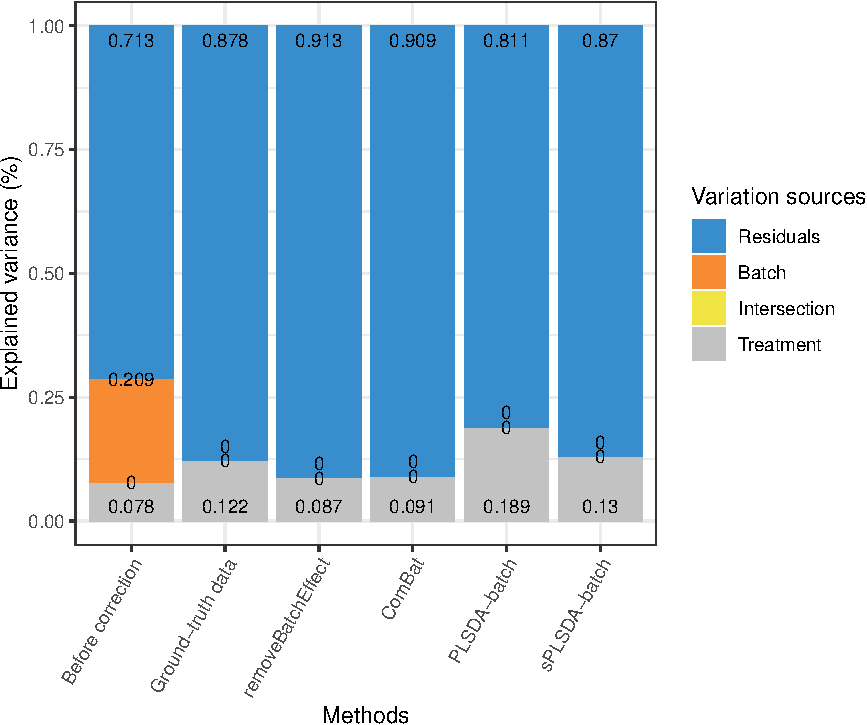
\includegraphics[width=0.7\linewidth]{PLSDAbatch_workflow_files/figure-latex/unnamed-chunk-99-1} 

}

\caption{Figure 1: Simulation studies (Gaussian distribution): comparison of explained variance before and after batch effect correction for the balanced batch × treatment design.}\label{fig:unnamed-chunk-99}
\end{figure}

We first considered the proportion of variance explained by treatment and batch effects before and after batch effect correction across all variables using pRDA. Efficient batch effect correction methods should generate data with a smaller proportion of batch associated variance and larger proportion of treatment variance compared to the original data. The figure shows that there was no intersection shared between treatment and batch variation with a balanced batch \(\times\) treatment design. All methods successfully removed batch variation, but PLSDA-batch and sPLSDA-batch preserved more proportion of treatment variance than removeBatchEffect and ComBat. In addition, the data corrected by sPLSDA-batch included almost as much proportion of treatment variance as the ground-truth data.

\begin{Shaded}
\begin{Highlighting}[]
\DocumentationTok{\#\#\#\#\#\#\#\#\#\#\#\#\#\#\#\#\#\#\#\#\#\#\#\#\#\#\#\#\#\#\#\#\#\#\#\#\#\#\#\#\#\#\#\#\#\#\#\#\#\#\#\#\#\#\#\#\#\#\#\#\#\#\#\#\#\#\#\#\#\#\#\#\#\#\#\#\#\#\#\#}
\CommentTok{\# individual variance (R2)}
\CommentTok{\# color}
\NormalTok{gcolor }\OtherTok{\textless{}{-}} \FunctionTok{c}\NormalTok{(}\FunctionTok{rep}\NormalTok{(}\FunctionTok{pb\_color}\NormalTok{(}\DecValTok{16}\NormalTok{), p\_trt\_relevant), }
            \FunctionTok{rep}\NormalTok{(}\FunctionTok{pb\_color}\NormalTok{(}\DecValTok{17}\NormalTok{), (p\_total }\SpecialCharTok{{-}}\NormalTok{ p\_trt\_relevant)))}
\NormalTok{gcolor[}\FunctionTok{intersect}\NormalTok{(true.trt, true.batch)] }\OtherTok{=} \FunctionTok{pb\_color}\NormalTok{(}\DecValTok{18}\NormalTok{)}
\NormalTok{gcolor[}\FunctionTok{setdiff}\NormalTok{(}\FunctionTok{seq\_len}\NormalTok{(p\_total), }\FunctionTok{union}\NormalTok{(true.trt, true.batch))] }\OtherTok{=} \FunctionTok{pb\_color}\NormalTok{(}\DecValTok{15}\NormalTok{)}

\NormalTok{xlabs }\OtherTok{=} \StringTok{\textquotesingle{}R2(variable, treatment)\textquotesingle{}}
\NormalTok{ylabs }\OtherTok{=} \StringTok{\textquotesingle{}R2(variable, batch)\textquotesingle{}}
\NormalTok{edgex }\OtherTok{=} \FloatTok{0.7}
\NormalTok{edgey }\OtherTok{=} \FloatTok{0.5}

\CommentTok{\# scatterplot}
\FunctionTok{par}\NormalTok{(}\AttributeTok{mfrow =} \FunctionTok{c}\NormalTok{(}\DecValTok{3}\NormalTok{,}\DecValTok{2}\NormalTok{))}
\FunctionTok{plot}\NormalTok{(}\FunctionTok{rowMeans}\NormalTok{(r2.trt.before), }\FunctionTok{rowMeans}\NormalTok{(r2.batch.before), }\AttributeTok{col =}\NormalTok{ gcolor, }
     \AttributeTok{xlab =}\NormalTok{ xlabs, }\AttributeTok{ylab =}\NormalTok{ ylabs, }\AttributeTok{pch =} \FunctionTok{as.numeric}\NormalTok{(}\FunctionTok{as.factor}\NormalTok{(gcolor)),}
     \AttributeTok{xlim =} \FunctionTok{c}\NormalTok{(}\DecValTok{0}\NormalTok{, edgex), }\AttributeTok{ylim =} \FunctionTok{c}\NormalTok{(}\DecValTok{0}\NormalTok{, edgey), }
     \AttributeTok{main =} \StringTok{\textquotesingle{}Before correction\textquotesingle{}}\NormalTok{, }\AttributeTok{cex =} \FloatTok{0.7}\NormalTok{)}
\FunctionTok{legend}\NormalTok{(}\StringTok{\textquotesingle{}topright\textquotesingle{}}\NormalTok{, }\AttributeTok{legend =} \FunctionTok{c}\NormalTok{(}\StringTok{\textquotesingle{}No effect\textquotesingle{}}\NormalTok{, }\StringTok{\textquotesingle{}Treatment only\textquotesingle{}}\NormalTok{, }
                              \StringTok{\textquotesingle{}Batch only\textquotesingle{}}\NormalTok{, }\StringTok{\textquotesingle{}Treatment \& batch\textquotesingle{}}\NormalTok{), }
       \AttributeTok{col =} \FunctionTok{pb\_color}\NormalTok{(}\DecValTok{15}\SpecialCharTok{:}\DecValTok{18}\NormalTok{), }\AttributeTok{pch =} \FunctionTok{seq\_len}\NormalTok{(}\DecValTok{4}\NormalTok{), }\AttributeTok{cex =} \FloatTok{0.8}\NormalTok{)}

\FunctionTok{plot}\NormalTok{(}\FunctionTok{rowMeans}\NormalTok{(r2.trt.clean), }\FunctionTok{rowMeans}\NormalTok{(r2.batch.clean), }\AttributeTok{col =}\NormalTok{ gcolor, }
     \AttributeTok{xlab =}\NormalTok{ xlabs, }\AttributeTok{ylab =}\NormalTok{ ylabs, }\AttributeTok{pch =} \FunctionTok{as.numeric}\NormalTok{(}\FunctionTok{as.factor}\NormalTok{(gcolor)),}
     \AttributeTok{xlim =} \FunctionTok{c}\NormalTok{(}\DecValTok{0}\NormalTok{, edgex), }\AttributeTok{ylim =} \FunctionTok{c}\NormalTok{(}\DecValTok{0}\NormalTok{, edgey), }
     \AttributeTok{main =} \StringTok{\textquotesingle{}Ground{-}truth data\textquotesingle{}}\NormalTok{, }\AttributeTok{cex =} \FloatTok{0.7}\NormalTok{)}
\FunctionTok{legend}\NormalTok{(}\StringTok{\textquotesingle{}topright\textquotesingle{}}\NormalTok{, }\AttributeTok{legend =} \FunctionTok{c}\NormalTok{(}\StringTok{\textquotesingle{}No effect\textquotesingle{}}\NormalTok{, }\StringTok{\textquotesingle{}Treatment only\textquotesingle{}}\NormalTok{, }
                              \StringTok{\textquotesingle{}Batch only\textquotesingle{}}\NormalTok{, }\StringTok{\textquotesingle{}Treatment \& batch\textquotesingle{}}\NormalTok{), }
       \AttributeTok{col =} \FunctionTok{pb\_color}\NormalTok{(}\DecValTok{15}\SpecialCharTok{:}\DecValTok{18}\NormalTok{), }\AttributeTok{pch =} \FunctionTok{seq\_len}\NormalTok{(}\DecValTok{4}\NormalTok{), }\AttributeTok{cex =} \FloatTok{0.8}\NormalTok{)}

\FunctionTok{plot}\NormalTok{(}\FunctionTok{rowMeans}\NormalTok{(r2.trt.rbe), }\FunctionTok{rowMeans}\NormalTok{(r2.batch.rbe), }\AttributeTok{col =}\NormalTok{ gcolor, }
     \AttributeTok{xlab =}\NormalTok{ xlabs, }\AttributeTok{ylab =}\NormalTok{ ylabs, }\AttributeTok{pch =} \FunctionTok{as.numeric}\NormalTok{(}\FunctionTok{as.factor}\NormalTok{(gcolor)),}
     \AttributeTok{xlim =} \FunctionTok{c}\NormalTok{(}\DecValTok{0}\NormalTok{, edgex), }\AttributeTok{ylim =} \FunctionTok{c}\NormalTok{(}\DecValTok{0}\NormalTok{, edgey), }
     \AttributeTok{main =} \StringTok{\textquotesingle{}removeBatchEffect\textquotesingle{}}\NormalTok{, }\AttributeTok{cex =} \FloatTok{0.7}\NormalTok{)}
\FunctionTok{legend}\NormalTok{(}\StringTok{\textquotesingle{}topright\textquotesingle{}}\NormalTok{, }\AttributeTok{legend =} \FunctionTok{c}\NormalTok{(}\StringTok{\textquotesingle{}No effect\textquotesingle{}}\NormalTok{, }\StringTok{\textquotesingle{}Treatment only\textquotesingle{}}\NormalTok{, }
                              \StringTok{\textquotesingle{}Batch only\textquotesingle{}}\NormalTok{, }\StringTok{\textquotesingle{}Treatment \& batch\textquotesingle{}}\NormalTok{), }
       \AttributeTok{col =} \FunctionTok{pb\_color}\NormalTok{(}\DecValTok{15}\SpecialCharTok{:}\DecValTok{18}\NormalTok{), }\AttributeTok{pch =} \FunctionTok{seq\_len}\NormalTok{(}\DecValTok{4}\NormalTok{), }\AttributeTok{cex =} \FloatTok{0.8}\NormalTok{)}

\FunctionTok{plot}\NormalTok{(}\FunctionTok{rowMeans}\NormalTok{(r2.trt.combat), }\FunctionTok{rowMeans}\NormalTok{(r2.batch.combat), }\AttributeTok{col =}\NormalTok{ gcolor, }
     \AttributeTok{xlab =}\NormalTok{ xlabs, }\AttributeTok{ylab =}\NormalTok{ ylabs, }\AttributeTok{pch =} \FunctionTok{as.numeric}\NormalTok{(}\FunctionTok{as.factor}\NormalTok{(gcolor)),}
     \AttributeTok{xlim =} \FunctionTok{c}\NormalTok{(}\DecValTok{0}\NormalTok{, edgex), }\AttributeTok{ylim =} \FunctionTok{c}\NormalTok{(}\DecValTok{0}\NormalTok{, edgey), }\AttributeTok{main =} \StringTok{\textquotesingle{}ComBat\textquotesingle{}}\NormalTok{, }\AttributeTok{cex =} \FloatTok{0.7}\NormalTok{)}
\FunctionTok{legend}\NormalTok{(}\StringTok{\textquotesingle{}topright\textquotesingle{}}\NormalTok{, }\AttributeTok{legend =} \FunctionTok{c}\NormalTok{(}\StringTok{\textquotesingle{}No effect\textquotesingle{}}\NormalTok{, }\StringTok{\textquotesingle{}Treatment only\textquotesingle{}}\NormalTok{, }
                              \StringTok{\textquotesingle{}Batch only\textquotesingle{}}\NormalTok{, }\StringTok{\textquotesingle{}Treatment \& batch\textquotesingle{}}\NormalTok{), }
       \AttributeTok{col =} \FunctionTok{pb\_color}\NormalTok{(}\DecValTok{15}\SpecialCharTok{:}\DecValTok{18}\NormalTok{), }\AttributeTok{pch =} \FunctionTok{seq\_len}\NormalTok{(}\DecValTok{4}\NormalTok{), }\AttributeTok{cex =} \FloatTok{0.8}\NormalTok{)}

\FunctionTok{plot}\NormalTok{(}\FunctionTok{rowMeans}\NormalTok{(r2.trt.plsdab), }\FunctionTok{rowMeans}\NormalTok{(r2.batch.plsdab), }\AttributeTok{col =}\NormalTok{ gcolor, }
     \AttributeTok{xlab =}\NormalTok{ xlabs, }\AttributeTok{ylab =}\NormalTok{ ylabs, }\AttributeTok{pch =} \FunctionTok{as.numeric}\NormalTok{(}\FunctionTok{as.factor}\NormalTok{(gcolor)),}
     \AttributeTok{xlim =} \FunctionTok{c}\NormalTok{(}\DecValTok{0}\NormalTok{, edgex), }\AttributeTok{ylim =} \FunctionTok{c}\NormalTok{(}\DecValTok{0}\NormalTok{, edgey), }\AttributeTok{main =} \StringTok{\textquotesingle{}PLSDA{-}batch\textquotesingle{}}\NormalTok{, }\AttributeTok{cex =} \FloatTok{0.7}\NormalTok{)}
\FunctionTok{legend}\NormalTok{(}\StringTok{\textquotesingle{}topright\textquotesingle{}}\NormalTok{, }\AttributeTok{legend =} \FunctionTok{c}\NormalTok{(}\StringTok{\textquotesingle{}No effect\textquotesingle{}}\NormalTok{, }\StringTok{\textquotesingle{}Treatment only\textquotesingle{}}\NormalTok{, }
                              \StringTok{\textquotesingle{}Batch only\textquotesingle{}}\NormalTok{, }\StringTok{\textquotesingle{}Treatment \& batch\textquotesingle{}}\NormalTok{), }
       \AttributeTok{col =} \FunctionTok{pb\_color}\NormalTok{(}\DecValTok{15}\SpecialCharTok{:}\DecValTok{18}\NormalTok{), }\AttributeTok{pch =} \FunctionTok{seq\_len}\NormalTok{(}\DecValTok{4}\NormalTok{), }\AttributeTok{cex =} \FloatTok{0.8}\NormalTok{)}

\FunctionTok{plot}\NormalTok{(}\FunctionTok{rowMeans}\NormalTok{(r2.trt.splsdab), }\FunctionTok{rowMeans}\NormalTok{(r2.batch.splsdab), }\AttributeTok{col =}\NormalTok{ gcolor, }
     \AttributeTok{xlab =}\NormalTok{ xlabs, }\AttributeTok{ylab =}\NormalTok{ ylabs, }\AttributeTok{pch =} \FunctionTok{as.numeric}\NormalTok{(}\FunctionTok{as.factor}\NormalTok{(gcolor)),}
     \AttributeTok{xlim =} \FunctionTok{c}\NormalTok{(}\DecValTok{0}\NormalTok{, edgex), }\AttributeTok{ylim =} \FunctionTok{c}\NormalTok{(}\DecValTok{0}\NormalTok{, edgey), }\AttributeTok{main =} \StringTok{\textquotesingle{}sPLSDA{-}batch\textquotesingle{}}\NormalTok{, }\AttributeTok{cex =} \FloatTok{0.7}\NormalTok{)}
\FunctionTok{legend}\NormalTok{(}\StringTok{\textquotesingle{}topright\textquotesingle{}}\NormalTok{, }\AttributeTok{legend =} \FunctionTok{c}\NormalTok{(}\StringTok{\textquotesingle{}No effect\textquotesingle{}}\NormalTok{, }\StringTok{\textquotesingle{}Treatment only\textquotesingle{}}\NormalTok{, }
                              \StringTok{\textquotesingle{}Batch only\textquotesingle{}}\NormalTok{, }\StringTok{\textquotesingle{}Treatment \& batch\textquotesingle{}}\NormalTok{), }
       \AttributeTok{col =} \FunctionTok{pb\_color}\NormalTok{(}\DecValTok{15}\SpecialCharTok{:}\DecValTok{18}\NormalTok{), }\AttributeTok{pch =} \FunctionTok{seq\_len}\NormalTok{(}\DecValTok{4}\NormalTok{), }\AttributeTok{cex =} \FloatTok{0.8}\NormalTok{)}
\end{Highlighting}
\end{Shaded}

\begin{figure}

{\centering 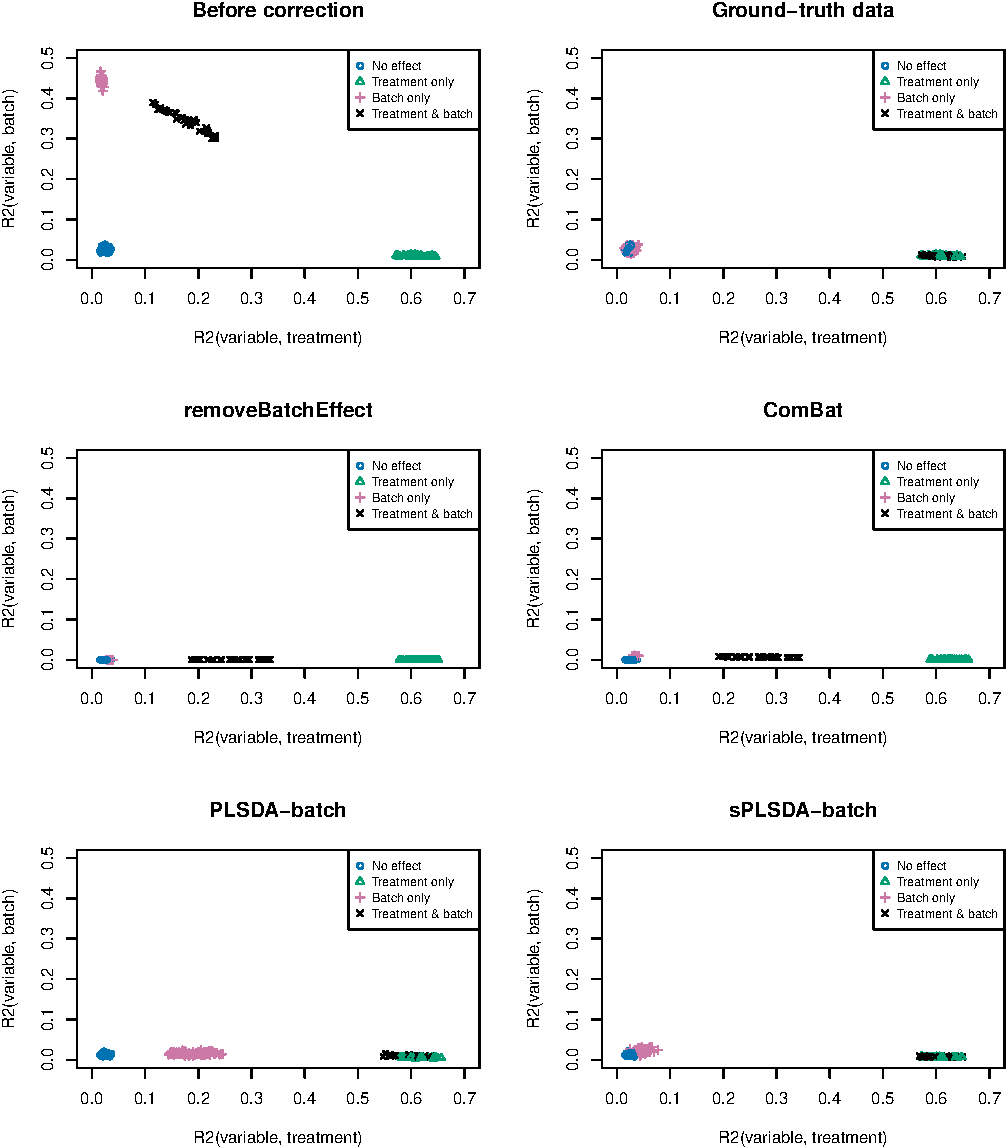
\includegraphics[width=1\linewidth]{PLSDAbatch_workflow_files/figure-latex/unnamed-chunk-100-1} 

}

\caption{Figure 2: Simulation studies (Gaussian distribution): R2 values for each microbial variable before and after batch effect correction for the balanced batch × treatment design.}\label{fig:unnamed-chunk-100}
\end{figure}

\begin{Shaded}
\begin{Highlighting}[]
\FunctionTok{par}\NormalTok{(}\AttributeTok{mfrow =} \FunctionTok{c}\NormalTok{(}\DecValTok{1}\NormalTok{,}\DecValTok{1}\NormalTok{))}
\end{Highlighting}
\end{Shaded}

We also estimated the proportion of variance explained by treatment and batch effects for each variable respectively using the \(R^2\) value. The variables assigned with both treatment and batch effects in the corrected data from removeBatchEffect and ComBat presented less proportion of treatment associated variance than in the ground truth data. This result agrees with the pRDA evaluation that these two methods do not preserve enough treatment variation. After PLSDA-batch correction, variables simulated with only batch effects displayed some amount of treatment variation, but only in the case where the batch effect variability among samples was high. sPLSDA-batch outperformed all methods, with results similar to the ground-truth data.

\begin{Shaded}
\begin{Highlighting}[]
\CommentTok{\# precision \& recall \& F1 (ANOVA \& sPLSDA)}
\DocumentationTok{\#\# mean}
\NormalTok{acc\_mean }\OtherTok{\textless{}{-}} \FunctionTok{rbind}\NormalTok{(}\FunctionTok{colMeans}\NormalTok{(precision\_limma), }\FunctionTok{colMeans}\NormalTok{(recall\_limma), }
                  \FunctionTok{colMeans}\NormalTok{(F1\_limma), }\FunctionTok{colMeans}\NormalTok{(precision\_splsda))}
\FunctionTok{rownames}\NormalTok{(acc\_mean) }\OtherTok{\textless{}{-}} \FunctionTok{c}\NormalTok{(}\StringTok{\textquotesingle{}Precision\textquotesingle{}}\NormalTok{, }\StringTok{\textquotesingle{}Recall\textquotesingle{}}\NormalTok{, }\StringTok{\textquotesingle{}F1\textquotesingle{}}\NormalTok{, }\StringTok{\textquotesingle{}Multivariate selection\textquotesingle{}}\NormalTok{)}
\FunctionTok{colnames}\NormalTok{(acc\_mean) }\OtherTok{\textless{}{-}} \FunctionTok{c}\NormalTok{(}\StringTok{\textquotesingle{}Before correction\textquotesingle{}}\NormalTok{, }\StringTok{\textquotesingle{}Ground{-}truth data\textquotesingle{}}\NormalTok{, }
                        \StringTok{\textquotesingle{}removeBatchEffect\textquotesingle{}}\NormalTok{, }\StringTok{\textquotesingle{}ComBat\textquotesingle{}}\NormalTok{, }
                        \StringTok{\textquotesingle{}PLSDA{-}batch\textquotesingle{}}\NormalTok{, }\StringTok{\textquotesingle{}sPLSDA{-}batch\textquotesingle{}}\NormalTok{)}
\NormalTok{acc\_mean }\OtherTok{\textless{}{-}} \FunctionTok{format}\NormalTok{(acc\_mean, }\AttributeTok{digits =} \DecValTok{2}\NormalTok{)}
\NormalTok{knitr}\SpecialCharTok{::}\FunctionTok{kable}\NormalTok{(acc\_mean, }\AttributeTok{caption =} \StringTok{\textquotesingle{}Table 3: Simulation studies (Gaussian distribution): summary of accuracy measures before and after batch correction for the balanced batch × treatment design (mean).\textquotesingle{}}\NormalTok{)}
\end{Highlighting}
\end{Shaded}

\begin{table}

\caption{\label{tab:unnamed-chunk-101}Table 3: Simulation studies (Gaussian distribution): summary of accuracy measures before and after batch correction for the balanced batch × treatment design (mean).}
\centering
\begin{tabular}[t]{l|l|l|l|l|l|l}
\hline
  & Before correction & Ground-truth data & removeBatchEffect & ComBat & PLSDA-batch & sPLSDA-batch\\
\hline
Precision & 0.98 & 0.95 & 0.94 & 0.93 & 0.56 & 0.86\\
\hline
Recall & 0.74 & 1.00 & 0.87 & 0.88 & 1.00 & 1.00\\
\hline
F1 & 0.84 & 0.98 & 0.89 & 0.89 & 0.68 & 0.92\\
\hline
Multivariate selection & 0.89 & 1.00 & 0.92 & 0.92 & 0.92 & 1.00\\
\hline
\end{tabular}
\end{table}

When considering the measures of accuracy with univariate one-way ANOVA, we observed that the corrected data from PLSDA-batch and sPLSDA-batch led to higher recall and lower precision than the data from removeBatchEffect and ComBat. However, the precision of sPLSDA-batch was competitive to removeBatchEffect and ComBat. Moreover, sPLSDA-batch achieved higher F1 scores and multivariate selection scores than removeBatchEffect and ComBat.

\begin{Shaded}
\begin{Highlighting}[]
\DocumentationTok{\#\# sd}
\NormalTok{acc\_sd }\OtherTok{\textless{}{-}} \FunctionTok{rbind}\NormalTok{(}\FunctionTok{apply}\NormalTok{(precision\_limma, }\DecValTok{2}\NormalTok{, sd), }\FunctionTok{apply}\NormalTok{(recall\_limma, }\DecValTok{2}\NormalTok{, sd), }
                \FunctionTok{apply}\NormalTok{(F1\_limma, }\DecValTok{2}\NormalTok{, sd), }\FunctionTok{apply}\NormalTok{(precision\_splsda, }\DecValTok{2}\NormalTok{, sd))}
\FunctionTok{rownames}\NormalTok{(acc\_sd) }\OtherTok{\textless{}{-}} \FunctionTok{c}\NormalTok{(}\StringTok{\textquotesingle{}Precision\textquotesingle{}}\NormalTok{, }\StringTok{\textquotesingle{}Recall\textquotesingle{}}\NormalTok{, }\StringTok{\textquotesingle{}F1\textquotesingle{}}\NormalTok{, }\StringTok{\textquotesingle{}Multivariate selection\textquotesingle{}}\NormalTok{)}
\FunctionTok{colnames}\NormalTok{(acc\_sd) }\OtherTok{\textless{}{-}} \FunctionTok{c}\NormalTok{(}\StringTok{\textquotesingle{}Before correction\textquotesingle{}}\NormalTok{, }\StringTok{\textquotesingle{}Ground{-}truth data\textquotesingle{}}\NormalTok{, }
                      \StringTok{\textquotesingle{}removeBatchEffect\textquotesingle{}}\NormalTok{, }\StringTok{\textquotesingle{}ComBat\textquotesingle{}}\NormalTok{, }
                      \StringTok{\textquotesingle{}PLSDA{-}batch\textquotesingle{}}\NormalTok{, }\StringTok{\textquotesingle{}sPLSDA{-}batch\textquotesingle{}}\NormalTok{)}
\NormalTok{acc\_sd }\OtherTok{\textless{}{-}} \FunctionTok{format}\NormalTok{(acc\_sd, }\AttributeTok{digits =} \DecValTok{1}\NormalTok{)}
\NormalTok{knitr}\SpecialCharTok{::}\FunctionTok{kable}\NormalTok{(acc\_sd, }\AttributeTok{caption =} \StringTok{\textquotesingle{}Table 4: Simulation studies (Gaussian distribution): summary of accuracy measures before and after batch correction for the balanced batch × treatment design (standard deviation).\textquotesingle{}}\NormalTok{)}
\end{Highlighting}
\end{Shaded}

\begin{table}

\caption{\label{tab:unnamed-chunk-102}Table 4: Simulation studies (Gaussian distribution): summary of accuracy measures before and after batch correction for the balanced batch × treatment design (standard deviation).}
\centering
\begin{tabular}[t]{l|l|l|l|l|l|l}
\hline
  & Before correction & Ground-truth data & removeBatchEffect & ComBat & PLSDA-batch & sPLSDA-batch\\
\hline
Precision & 0.021 & 0.031 & 0.151 & 0.160 & 0.252 & 0.110\\
\hline
Recall & 0.095 & 0.000 & 0.098 & 0.098 & 0.021 & 0.000\\
\hline
F1 & 0.065 & 0.016 & 0.118 & 0.124 & 0.200 & 0.068\\
\hline
Multivariate selection & 0.061 & 0.000 & 0.068 & 0.069 & 0.123 & 0.005\\
\hline
\end{tabular}
\end{table}

The standard deviations of the multivariate selection scores were all smaller than the univariate selection scores for the different corrected data, indicating a better stability of the variables selected by multivariate sPLSDA compared to the one-way ANOVA univariate selection.

\hypertarget{unbalanced-batch-times-treatment-design}{%
\subsection{\texorpdfstring{Unbalanced batch \(\times\) treatment design}{Unbalanced batch \textbackslash times treatment design}}\label{unbalanced-batch-times-treatment-design}}

The unbalanced design had 4 and 16 samples from batch1 and batch2 respectively in trt1, 16 and 4 samples from batch1 and batch2 in trt2 (see the table below).

\textbf{Table 5: Unbalanced batch \(\times\) treatment design} in the simulation study

\begin{longtable}[]{@{}ccc@{}}
\toprule()
& Trt1 & Trt2 \\
\midrule()
\endhead
Batch1 & 4 & 16 \\
Batch2 & 16 & 4 \\
\bottomrule()
\end{longtable}

\begin{Shaded}
\begin{Highlighting}[]
\NormalTok{nitr }\OtherTok{\textless{}{-}} \DecValTok{50}
\NormalTok{p\_total }\OtherTok{\textless{}{-}} \DecValTok{300}
\NormalTok{p\_trt\_relevant }\OtherTok{\textless{}{-}} \DecValTok{60}
\NormalTok{p\_bat\_relevant }\OtherTok{\textless{}{-}} \DecValTok{150}

\CommentTok{\# global variance (RDA)}
\NormalTok{gvar.before }\OtherTok{\textless{}{-}}\NormalTok{ gvar.clean }\OtherTok{\textless{}{-}}\NormalTok{ gvar.rbe }\OtherTok{\textless{}{-}}\NormalTok{ gvar.combat }\OtherTok{\textless{}{-}} 
\NormalTok{  gvar.wplsdab }\OtherTok{\textless{}{-}}\NormalTok{ gvar.swplsdab }\OtherTok{\textless{}{-}}\NormalTok{ gvar.plsdab }\OtherTok{\textless{}{-}} 
\NormalTok{  gvar.splsdab }\OtherTok{\textless{}{-}} \FunctionTok{data.frame}\NormalTok{(}\AttributeTok{treatment =} \ConstantTok{NA}\NormalTok{, }\AttributeTok{batch =} \ConstantTok{NA}\NormalTok{,  }
                             \AttributeTok{intersection =} \ConstantTok{NA}\NormalTok{, }
                             \AttributeTok{residual =} \ConstantTok{NA}\NormalTok{)}

\CommentTok{\# individual variance (R2)}
\NormalTok{r2.trt.before }\OtherTok{\textless{}{-}}\NormalTok{ r2.trt.clean }\OtherTok{\textless{}{-}}\NormalTok{ r2.trt.rbe  }\OtherTok{\textless{}{-}}\NormalTok{ r2.trt.combat }\OtherTok{\textless{}{-}} 
\NormalTok{  r2.trt.wplsdab }\OtherTok{\textless{}{-}}\NormalTok{ r2.trt.swplsdab }\OtherTok{\textless{}{-}} \FunctionTok{data.frame}\NormalTok{(}\FunctionTok{matrix}\NormalTok{(}\ConstantTok{NA}\NormalTok{, }\AttributeTok{nrow =}\NormalTok{ p\_total, }
                                                         \AttributeTok{ncol =}\NormalTok{ nitr))}
\NormalTok{r2.batch.before }\OtherTok{\textless{}{-}}\NormalTok{ r2.batch.clean }\OtherTok{\textless{}{-}}\NormalTok{ r2.batch.rbe  }\OtherTok{\textless{}{-}}\NormalTok{ r2.batch.combat }\OtherTok{\textless{}{-}} 
\NormalTok{  r2.batch.wplsdab }\OtherTok{\textless{}{-}}\NormalTok{ r2.batch.swplsdab }\OtherTok{\textless{}{-}} \FunctionTok{data.frame}\NormalTok{(}\FunctionTok{matrix}\NormalTok{(}\ConstantTok{NA}\NormalTok{, }\AttributeTok{nrow =}\NormalTok{ p\_total, }
                                                             \AttributeTok{ncol =}\NormalTok{ nitr))}

\CommentTok{\# precision \& recall \& F1 (ANOVA)}
\NormalTok{precision\_limma }\OtherTok{\textless{}{-}}\NormalTok{ recall\_limma }\OtherTok{\textless{}{-}}\NormalTok{ F1\_limma }\OtherTok{\textless{}{-}} 
  \FunctionTok{data.frame}\NormalTok{(}\AttributeTok{before =} \ConstantTok{NA}\NormalTok{, }\AttributeTok{clean =} \ConstantTok{NA}\NormalTok{, }\AttributeTok{rbe =} \ConstantTok{NA}\NormalTok{, }\AttributeTok{combat =} \ConstantTok{NA}\NormalTok{, }
             \AttributeTok{wplsda\_batch =} \ConstantTok{NA}\NormalTok{, }\AttributeTok{swplsda\_batch =} \ConstantTok{NA}\NormalTok{)}

\CommentTok{\# precision \& recall \& F1 (sPLSDA)}
\NormalTok{precision\_splsda }\OtherTok{\textless{}{-}}\NormalTok{ recall\_splsda }\OtherTok{\textless{}{-}}\NormalTok{ F1\_splsda }\OtherTok{\textless{}{-}} 
  \FunctionTok{data.frame}\NormalTok{(}\AttributeTok{before =} \ConstantTok{NA}\NormalTok{, }\AttributeTok{clean =} \ConstantTok{NA}\NormalTok{, }\AttributeTok{rbe =} \ConstantTok{NA}\NormalTok{, }\AttributeTok{combat =} \ConstantTok{NA}\NormalTok{, }
             \AttributeTok{wplsda\_batch =} \ConstantTok{NA}\NormalTok{, }\AttributeTok{swplsda\_batch =} \ConstantTok{NA}\NormalTok{)}

\ControlFlowTok{for}\NormalTok{(i }\ControlFlowTok{in} \FunctionTok{seq\_len}\NormalTok{(nitr))\{}
  \DocumentationTok{\#\#\# initial setup }\AlertTok{\#\#\#}
\NormalTok{  simulation }\OtherTok{\textless{}{-}} \FunctionTok{simData\_Gaussian}\NormalTok{(}\AttributeTok{mean.batch =} \DecValTok{7}\NormalTok{, }\AttributeTok{sd.batch =} \DecValTok{8}\NormalTok{, }
                                 \AttributeTok{mean.trt =} \DecValTok{3}\NormalTok{, }\AttributeTok{sd.trt =} \DecValTok{2}\NormalTok{, }
                                 \AttributeTok{N =} \DecValTok{40}\NormalTok{, }\AttributeTok{p\_total =} \DecValTok{300}\NormalTok{, }
                                 \AttributeTok{p\_trt\_relevant =} \DecValTok{60}\NormalTok{, }
                                 \AttributeTok{p\_bat\_relevant =} \DecValTok{150}\NormalTok{, }
                                 \AttributeTok{percentage\_overlap\_samples =} \FloatTok{0.2}\NormalTok{,}
                                 \AttributeTok{percentage\_overlap\_variables =} \FloatTok{0.5}\NormalTok{, }\AttributeTok{seeds =}\NormalTok{ i)}
  
\NormalTok{  X }\OtherTok{\textless{}{-}}\NormalTok{ simulation}\SpecialCharTok{$}\NormalTok{data}
\NormalTok{  trt }\OtherTok{\textless{}{-}}\NormalTok{ simulation}\SpecialCharTok{$}\NormalTok{Y.trt}
\NormalTok{  batch }\OtherTok{\textless{}{-}}\NormalTok{ simulation}\SpecialCharTok{$}\NormalTok{Y.bat}
\NormalTok{  true.trt }\OtherTok{\textless{}{-}}\NormalTok{ simulation}\SpecialCharTok{$}\NormalTok{true.trt}
\NormalTok{  true.batch }\OtherTok{\textless{}{-}}\NormalTok{ simulation}\SpecialCharTok{$}\NormalTok{true.batch}
  
\NormalTok{  Batch\_Trt.factors }\OtherTok{\textless{}{-}} \FunctionTok{data.frame}\NormalTok{(}\AttributeTok{Batch =}\NormalTok{ batch, }\AttributeTok{Treatment =}\NormalTok{ trt)}
  
  \DocumentationTok{\#\#\# Before correction }\AlertTok{\#\#\#}
  \CommentTok{\# global variance (RDA)}
\NormalTok{  rda.before }\OtherTok{=} \FunctionTok{varpart}\NormalTok{(}\FunctionTok{scale}\NormalTok{(X), }\SpecialCharTok{\textasciitilde{}}\NormalTok{ Treatment, }\SpecialCharTok{\textasciitilde{}}\NormalTok{ Batch, }\AttributeTok{data =}\NormalTok{ Batch\_Trt.factors)}
\NormalTok{  gvar.before[i, ] }\OtherTok{\textless{}{-}}\NormalTok{ rda.before}\SpecialCharTok{$}\NormalTok{part}\SpecialCharTok{$}\NormalTok{indfract}\SpecialCharTok{$}\NormalTok{Adj.R.squared}
  
  \CommentTok{\# individual variance (R2)}
\NormalTok{  indiv.trt.before }\OtherTok{\textless{}{-}} \FunctionTok{c}\NormalTok{()}
\NormalTok{  indiv.batch.before }\OtherTok{\textless{}{-}} \FunctionTok{c}\NormalTok{()}
  \ControlFlowTok{for}\NormalTok{(c }\ControlFlowTok{in} \FunctionTok{seq\_len}\NormalTok{(}\FunctionTok{ncol}\NormalTok{(X)))\{}
\NormalTok{    fit.res1 }\OtherTok{\textless{}{-}} \FunctionTok{lm}\NormalTok{(}\FunctionTok{scale}\NormalTok{(X)[ ,c] }\SpecialCharTok{\textasciitilde{}}\NormalTok{ trt)}
\NormalTok{    fit.summary1 }\OtherTok{\textless{}{-}} \FunctionTok{summary}\NormalTok{(fit.res1)}
\NormalTok{    fit.res2 }\OtherTok{\textless{}{-}} \FunctionTok{lm}\NormalTok{(}\FunctionTok{scale}\NormalTok{(X)[ ,c] }\SpecialCharTok{\textasciitilde{}}\NormalTok{ batch)}
\NormalTok{    fit.summary2 }\OtherTok{\textless{}{-}} \FunctionTok{summary}\NormalTok{(fit.res2)}
\NormalTok{    indiv.trt.before }\OtherTok{\textless{}{-}} \FunctionTok{c}\NormalTok{(indiv.trt.before, fit.summary1}\SpecialCharTok{$}\NormalTok{r.squared)}
\NormalTok{    indiv.batch.before }\OtherTok{\textless{}{-}} \FunctionTok{c}\NormalTok{(indiv.batch.before, fit.summary2}\SpecialCharTok{$}\NormalTok{r.squared)}
\NormalTok{  \}}
\NormalTok{  r2.trt.before[ ,i] }\OtherTok{\textless{}{-}}\NormalTok{  indiv.trt.before}
\NormalTok{  r2.batch.before[ ,i] }\OtherTok{\textless{}{-}}\NormalTok{  indiv.batch.before}
  
  \CommentTok{\# precision \& recall \& F1 (ANOVA)}
\NormalTok{  fit.before }\OtherTok{\textless{}{-}} \FunctionTok{lmFit}\NormalTok{(}\FunctionTok{t}\NormalTok{(}\FunctionTok{scale}\NormalTok{(X)), }\AttributeTok{design =} \FunctionTok{model.matrix}\NormalTok{( }\SpecialCharTok{\textasciitilde{}} \DecValTok{0} \SpecialCharTok{+} \FunctionTok{as.factor}\NormalTok{(trt)))}
\NormalTok{  fit.before }\OtherTok{\textless{}{-}} \FunctionTok{contrasts.fit}\NormalTok{(fit.before, }\AttributeTok{contrasts =} \FunctionTok{c}\NormalTok{(}\DecValTok{1}\NormalTok{,}\SpecialCharTok{{-}}\DecValTok{1}\NormalTok{))}
\NormalTok{  fit.result.before }\OtherTok{\textless{}{-}} \FunctionTok{topTable}\NormalTok{(}\FunctionTok{eBayes}\NormalTok{(fit.before), }\AttributeTok{number =}\NormalTok{ p\_total)}
\NormalTok{  otu.sig.before }\OtherTok{\textless{}{-}} 
    \FunctionTok{rownames}\NormalTok{(fit.result.before)[fit.result.before}\SpecialCharTok{$}\NormalTok{adj.P.Val }\SpecialCharTok{\textless{}=} \FloatTok{0.05}\NormalTok{]}
  
\NormalTok{  precision\_limma.before }\OtherTok{\textless{}{-}} \FunctionTok{length}\NormalTok{(}\FunctionTok{intersect}\NormalTok{(true.trt, otu.sig.before))}\SpecialCharTok{/}
    \FunctionTok{length}\NormalTok{(otu.sig.before)}
\NormalTok{  recall\_limma.before }\OtherTok{\textless{}{-}} \FunctionTok{length}\NormalTok{(}\FunctionTok{intersect}\NormalTok{(true.trt, otu.sig.before))}\SpecialCharTok{/}
    \FunctionTok{length}\NormalTok{(true.trt)}
\NormalTok{  F1\_limma.before }\OtherTok{\textless{}{-}}\NormalTok{ (}\DecValTok{2}\SpecialCharTok{*}\NormalTok{precision\_limma.before}\SpecialCharTok{*}\NormalTok{recall\_limma.before)}\SpecialCharTok{/}
\NormalTok{    (precision\_limma.before }\SpecialCharTok{+}\NormalTok{ recall\_limma.before)}
  
  \DocumentationTok{\#\# replace NA value with 0}
  \ControlFlowTok{if}\NormalTok{(precision\_limma.before }\SpecialCharTok{==} \StringTok{\textquotesingle{}NaN\textquotesingle{}}\NormalTok{)\{}
\NormalTok{    precision\_limma.before }\OtherTok{=} \DecValTok{0}
\NormalTok{  \}}
  \ControlFlowTok{if}\NormalTok{(F1\_limma.before }\SpecialCharTok{==} \StringTok{\textquotesingle{}NaN\textquotesingle{}}\NormalTok{)\{}
\NormalTok{    F1\_limma.before }\OtherTok{=} \DecValTok{0}
\NormalTok{  \}}
  
  \CommentTok{\# precision \& recall \& F1 (sPLSDA)}
\NormalTok{  fit.before\_splsda }\OtherTok{\textless{}{-}} \FunctionTok{splsda}\NormalTok{(}\AttributeTok{X =}\NormalTok{ X, }\AttributeTok{Y =}\NormalTok{ trt, }
                              \AttributeTok{ncomp =} \DecValTok{1}\NormalTok{, }\AttributeTok{keepX =} \FunctionTok{length}\NormalTok{(true.trt))}
\NormalTok{  otu.dcn.before }\OtherTok{\textless{}{-}} \FunctionTok{which}\NormalTok{(fit.before\_splsda}\SpecialCharTok{$}\NormalTok{loadings}\SpecialCharTok{$}\NormalTok{X[,}\DecValTok{1}\NormalTok{] }\SpecialCharTok{!=} \DecValTok{0}\NormalTok{)}
  
\NormalTok{  precision\_splsda.before }\OtherTok{\textless{}{-}} \FunctionTok{length}\NormalTok{(}\FunctionTok{intersect}\NormalTok{(true.trt, otu.dcn.before))}\SpecialCharTok{/}
    \FunctionTok{length}\NormalTok{(otu.dcn.before)}
\NormalTok{  recall\_splsda.before }\OtherTok{\textless{}{-}} \FunctionTok{length}\NormalTok{(}\FunctionTok{intersect}\NormalTok{(true.trt, otu.dcn.before))}\SpecialCharTok{/}
    \FunctionTok{length}\NormalTok{(true.trt)}
\NormalTok{  F1\_splsda.before }\OtherTok{\textless{}{-}}\NormalTok{ (}\DecValTok{2}\SpecialCharTok{*}\NormalTok{precision\_splsda.before}\SpecialCharTok{*}\NormalTok{recall\_splsda.before)}\SpecialCharTok{/}
\NormalTok{    (precision\_splsda.before }\SpecialCharTok{+}\NormalTok{ recall\_splsda.before)}
  
  \DocumentationTok{\#\# replace NA value with 0}
  \ControlFlowTok{if}\NormalTok{(F1\_splsda.before }\SpecialCharTok{==} \StringTok{\textquotesingle{}NaN\textquotesingle{}}\NormalTok{)\{}
\NormalTok{    F1\_splsda.before }\OtherTok{=} \DecValTok{0}
\NormalTok{  \}}
  
  \DocumentationTok{\#\#\#\#\#\#\#\#\#\#\#\#\#\#\#\#\#\#\#\#\#\#\#\#\#\#\#\#\#\#\#\#\#\#\#\#\#\#\#\#\#\#\#\#\#\#\#\#\#\#\#\#\#\#\#\#\#\#\#\#\#\#\#\#\#\#\#\#\#\#\#\#\#\#\#\#\#\#}
  \DocumentationTok{\#\#\# Ground{-}truth data }\AlertTok{\#\#\#}
\NormalTok{  X.clean }\OtherTok{\textless{}{-}}\NormalTok{ simulation}\SpecialCharTok{$}\NormalTok{cleanData}
  \CommentTok{\# global variance (RDA)}
\NormalTok{  rda.clean }\OtherTok{=} \FunctionTok{varpart}\NormalTok{(}\FunctionTok{scale}\NormalTok{(X.clean), }\SpecialCharTok{\textasciitilde{}}\NormalTok{ Treatment, }\SpecialCharTok{\textasciitilde{}}\NormalTok{ Batch, }
                      \AttributeTok{data =}\NormalTok{ Batch\_Trt.factors)}
\NormalTok{  gvar.clean[i, ] }\OtherTok{\textless{}{-}}\NormalTok{ rda.clean}\SpecialCharTok{$}\NormalTok{part}\SpecialCharTok{$}\NormalTok{indfract}\SpecialCharTok{$}\NormalTok{Adj.R.squared}
  
  \CommentTok{\# individual variance (R2)}
\NormalTok{  indiv.trt.clean }\OtherTok{\textless{}{-}} \FunctionTok{c}\NormalTok{()}
\NormalTok{  indiv.batch.clean }\OtherTok{\textless{}{-}} \FunctionTok{c}\NormalTok{()}
  \ControlFlowTok{for}\NormalTok{(c }\ControlFlowTok{in} \FunctionTok{seq\_len}\NormalTok{(}\FunctionTok{ncol}\NormalTok{(X.clean)))\{}
\NormalTok{    fit.res1 }\OtherTok{\textless{}{-}} \FunctionTok{lm}\NormalTok{(}\FunctionTok{scale}\NormalTok{(X.clean)[ ,c] }\SpecialCharTok{\textasciitilde{}}\NormalTok{ trt)}
\NormalTok{    fit.summary1 }\OtherTok{\textless{}{-}} \FunctionTok{summary}\NormalTok{(fit.res1)}
\NormalTok{    fit.res2 }\OtherTok{\textless{}{-}} \FunctionTok{lm}\NormalTok{(}\FunctionTok{scale}\NormalTok{(X.clean)[ ,c] }\SpecialCharTok{\textasciitilde{}}\NormalTok{ batch)}
\NormalTok{    fit.summary2 }\OtherTok{\textless{}{-}} \FunctionTok{summary}\NormalTok{(fit.res2)}
\NormalTok{    indiv.trt.clean }\OtherTok{\textless{}{-}} \FunctionTok{c}\NormalTok{(indiv.trt.clean, fit.summary1}\SpecialCharTok{$}\NormalTok{r.squared)}
\NormalTok{    indiv.batch.clean }\OtherTok{\textless{}{-}} \FunctionTok{c}\NormalTok{(indiv.batch.clean, fit.summary2}\SpecialCharTok{$}\NormalTok{r.squared)}
\NormalTok{  \}}
\NormalTok{  r2.trt.clean[ ,i] }\OtherTok{\textless{}{-}}\NormalTok{  indiv.trt.clean}
\NormalTok{  r2.batch.clean[ ,i] }\OtherTok{\textless{}{-}}\NormalTok{  indiv.batch.clean}
  
  \CommentTok{\# precision \& recall \& F1 (ANOVA)}
\NormalTok{  fit.clean }\OtherTok{\textless{}{-}} \FunctionTok{lmFit}\NormalTok{(}\FunctionTok{t}\NormalTok{(}\FunctionTok{scale}\NormalTok{(X.clean)), }
                     \AttributeTok{design =} \FunctionTok{model.matrix}\NormalTok{( }\SpecialCharTok{\textasciitilde{}} \DecValTok{0} \SpecialCharTok{+} \FunctionTok{as.factor}\NormalTok{(trt)))}
\NormalTok{  fit.clean }\OtherTok{\textless{}{-}} \FunctionTok{contrasts.fit}\NormalTok{(fit.clean, }\AttributeTok{contrasts =} \FunctionTok{c}\NormalTok{(}\DecValTok{1}\NormalTok{,}\SpecialCharTok{{-}}\DecValTok{1}\NormalTok{))}
\NormalTok{  fit.result.clean }\OtherTok{\textless{}{-}} \FunctionTok{topTable}\NormalTok{(}\FunctionTok{eBayes}\NormalTok{(fit.clean), }\AttributeTok{number =}\NormalTok{ p\_total)}
\NormalTok{  otu.sig.clean }\OtherTok{\textless{}{-}} 
    \FunctionTok{rownames}\NormalTok{(fit.result.clean)[fit.result.clean}\SpecialCharTok{$}\NormalTok{adj.P.Val }\SpecialCharTok{\textless{}=} \FloatTok{0.05}\NormalTok{]}
  
\NormalTok{  precision\_limma.clean }\OtherTok{\textless{}{-}} \FunctionTok{length}\NormalTok{(}\FunctionTok{intersect}\NormalTok{(true.trt, otu.sig.clean))}\SpecialCharTok{/}
    \FunctionTok{length}\NormalTok{(otu.sig.clean)}
\NormalTok{  recall\_limma.clean }\OtherTok{\textless{}{-}} \FunctionTok{length}\NormalTok{(}\FunctionTok{intersect}\NormalTok{(true.trt, otu.sig.clean))}\SpecialCharTok{/}
    \FunctionTok{length}\NormalTok{(true.trt)}
\NormalTok{  F1\_limma.clean }\OtherTok{\textless{}{-}}\NormalTok{ (}\DecValTok{2}\SpecialCharTok{*}\NormalTok{precision\_limma.clean}\SpecialCharTok{*}\NormalTok{recall\_limma.clean)}\SpecialCharTok{/}
\NormalTok{    (precision\_limma.clean }\SpecialCharTok{+}\NormalTok{ recall\_limma.clean)}
  
  \DocumentationTok{\#\# replace NA value with 0}
  \ControlFlowTok{if}\NormalTok{(precision\_limma.clean }\SpecialCharTok{==} \StringTok{\textquotesingle{}NaN\textquotesingle{}}\NormalTok{)\{}
\NormalTok{    precision\_limma.clean }\OtherTok{=} \DecValTok{0}
\NormalTok{  \}}
  \ControlFlowTok{if}\NormalTok{(F1\_limma.clean }\SpecialCharTok{==} \StringTok{\textquotesingle{}NaN\textquotesingle{}}\NormalTok{)\{}
\NormalTok{    F1\_limma.clean }\OtherTok{=} \DecValTok{0}
\NormalTok{  \}}
  
  \CommentTok{\# precision \& recall \& F1 (sPLSDA)}
\NormalTok{  fit.clean\_splsda }\OtherTok{\textless{}{-}} \FunctionTok{splsda}\NormalTok{(}\AttributeTok{X =}\NormalTok{ X.clean, }\AttributeTok{Y =}\NormalTok{ trt, }\AttributeTok{ncomp =} \DecValTok{1}\NormalTok{, }
                             \AttributeTok{keepX =} \FunctionTok{length}\NormalTok{(true.trt))}
\NormalTok{  otu.dcn.clean }\OtherTok{\textless{}{-}} \FunctionTok{which}\NormalTok{(fit.clean\_splsda}\SpecialCharTok{$}\NormalTok{loadings}\SpecialCharTok{$}\NormalTok{X[ ,}\DecValTok{1}\NormalTok{] }\SpecialCharTok{!=} \DecValTok{0}\NormalTok{)}
  
\NormalTok{  precision\_splsda.clean }\OtherTok{\textless{}{-}} \FunctionTok{length}\NormalTok{(}\FunctionTok{intersect}\NormalTok{(true.trt, otu.dcn.clean))}\SpecialCharTok{/}
    \FunctionTok{length}\NormalTok{(otu.dcn.clean)}
\NormalTok{  recall\_splsda.clean }\OtherTok{\textless{}{-}} \FunctionTok{length}\NormalTok{(}\FunctionTok{intersect}\NormalTok{(true.trt, otu.dcn.clean))}\SpecialCharTok{/}
    \FunctionTok{length}\NormalTok{(true.trt)}
\NormalTok{  F1\_splsda.clean }\OtherTok{\textless{}{-}}\NormalTok{ (}\DecValTok{2}\SpecialCharTok{*}\NormalTok{precision\_splsda.clean}\SpecialCharTok{*}\NormalTok{recall\_splsda.clean)}\SpecialCharTok{/}
\NormalTok{    (precision\_splsda.clean }\SpecialCharTok{+}\NormalTok{ recall\_splsda.clean)}
  
  \DocumentationTok{\#\# replace NA value with 0}
  \ControlFlowTok{if}\NormalTok{(F1\_splsda.clean }\SpecialCharTok{==} \StringTok{\textquotesingle{}NaN\textquotesingle{}}\NormalTok{)\{}
\NormalTok{    F1\_splsda.clean }\OtherTok{=} \DecValTok{0}
\NormalTok{  \}}
  
  \DocumentationTok{\#\#\#\#\#\#\#\#\#\#\#\#\#\#\#\#\#\#\#\#\#\#\#\#\#\#\#\#\#\#\#\#\#\#\#\#\#\#\#\#\#\#\#\#\#\#\#\#\#\#\#\#\#\#\#\#\#\#\#\#\#\#\#\#\#\#\#\#\#\#\#\#\#\#\#\#\#\#}
  \DocumentationTok{\#\#\# removeBatchEffect corrected data }\AlertTok{\#\#\#}
\NormalTok{  X.rbe }\OtherTok{\textless{}{-}}\FunctionTok{t}\NormalTok{(}\FunctionTok{removeBatchEffect}\NormalTok{(}\FunctionTok{t}\NormalTok{(X), }\AttributeTok{batch =}\NormalTok{ batch, }
                              \AttributeTok{design =} \FunctionTok{model.matrix}\NormalTok{( }\SpecialCharTok{\textasciitilde{}} \DecValTok{0} \SpecialCharTok{+} \FunctionTok{as.factor}\NormalTok{(trt))))}
  
  \CommentTok{\# global variance (RDA)}
\NormalTok{  rda.rbe }\OtherTok{=} \FunctionTok{varpart}\NormalTok{(}\FunctionTok{scale}\NormalTok{(X.rbe), }\SpecialCharTok{\textasciitilde{}}\NormalTok{ Treatment, }\SpecialCharTok{\textasciitilde{}}\NormalTok{ Batch, }
                    \AttributeTok{data =}\NormalTok{ Batch\_Trt.factors)}
\NormalTok{  gvar.rbe[i, ] }\OtherTok{\textless{}{-}}\NormalTok{ rda.rbe}\SpecialCharTok{$}\NormalTok{part}\SpecialCharTok{$}\NormalTok{indfract}\SpecialCharTok{$}\NormalTok{Adj.R.squared}
  
  \CommentTok{\# individual variance (R2)}
\NormalTok{  indiv.trt.rbe }\OtherTok{\textless{}{-}} \FunctionTok{c}\NormalTok{()}
\NormalTok{  indiv.batch.rbe }\OtherTok{\textless{}{-}} \FunctionTok{c}\NormalTok{()}
  \ControlFlowTok{for}\NormalTok{(c }\ControlFlowTok{in} \FunctionTok{seq\_len}\NormalTok{(}\FunctionTok{ncol}\NormalTok{(X.rbe)))\{}
\NormalTok{    fit.res1 }\OtherTok{\textless{}{-}} \FunctionTok{lm}\NormalTok{(}\FunctionTok{scale}\NormalTok{(X.rbe)[ ,c] }\SpecialCharTok{\textasciitilde{}}\NormalTok{ trt)}
\NormalTok{    fit.summary1 }\OtherTok{\textless{}{-}} \FunctionTok{summary}\NormalTok{(fit.res1)}
\NormalTok{    fit.res2 }\OtherTok{\textless{}{-}} \FunctionTok{lm}\NormalTok{(}\FunctionTok{scale}\NormalTok{(X.rbe)[ ,c] }\SpecialCharTok{\textasciitilde{}}\NormalTok{ batch)}
\NormalTok{    fit.summary2 }\OtherTok{\textless{}{-}} \FunctionTok{summary}\NormalTok{(fit.res2)}
\NormalTok{    indiv.trt.rbe }\OtherTok{\textless{}{-}} \FunctionTok{c}\NormalTok{(indiv.trt.rbe, fit.summary1}\SpecialCharTok{$}\NormalTok{r.squared)}
\NormalTok{    indiv.batch.rbe }\OtherTok{\textless{}{-}} \FunctionTok{c}\NormalTok{(indiv.batch.rbe, fit.summary2}\SpecialCharTok{$}\NormalTok{r.squared)}
\NormalTok{  \}}
\NormalTok{  r2.trt.rbe[ ,i] }\OtherTok{\textless{}{-}}\NormalTok{  indiv.trt.rbe}
\NormalTok{  r2.batch.rbe[ ,i] }\OtherTok{\textless{}{-}}\NormalTok{  indiv.batch.rbe}
  
  \CommentTok{\# precision \& recall \& F1 (ANOVA)}
\NormalTok{  fit.rbe }\OtherTok{\textless{}{-}} \FunctionTok{lmFit}\NormalTok{(}\FunctionTok{t}\NormalTok{(}\FunctionTok{scale}\NormalTok{(X.rbe)), }
                   \AttributeTok{design =} \FunctionTok{model.matrix}\NormalTok{( }\SpecialCharTok{\textasciitilde{}} \DecValTok{0} \SpecialCharTok{+} \FunctionTok{as.factor}\NormalTok{(trt)))}
\NormalTok{  fit.rbe }\OtherTok{\textless{}{-}} \FunctionTok{contrasts.fit}\NormalTok{(fit.rbe, }\AttributeTok{contrasts =} \FunctionTok{c}\NormalTok{(}\DecValTok{1}\NormalTok{,}\SpecialCharTok{{-}}\DecValTok{1}\NormalTok{))}
\NormalTok{  fit.result.rbe }\OtherTok{\textless{}{-}} \FunctionTok{topTable}\NormalTok{(}\FunctionTok{eBayes}\NormalTok{(fit.rbe), }\AttributeTok{number =}\NormalTok{ p\_total)}
\NormalTok{  otu.sig.rbe }\OtherTok{\textless{}{-}} \FunctionTok{rownames}\NormalTok{(fit.result.rbe)[fit.result.rbe}\SpecialCharTok{$}\NormalTok{adj.P.Val }\SpecialCharTok{\textless{}=} \FloatTok{0.05}\NormalTok{]}
  
\NormalTok{  precision\_limma.rbe }\OtherTok{\textless{}{-}} \FunctionTok{length}\NormalTok{(}\FunctionTok{intersect}\NormalTok{(true.trt, otu.sig.rbe))}\SpecialCharTok{/}
    \FunctionTok{length}\NormalTok{(otu.sig.rbe)}
\NormalTok{  recall\_limma.rbe }\OtherTok{\textless{}{-}} \FunctionTok{length}\NormalTok{(}\FunctionTok{intersect}\NormalTok{(true.trt, otu.sig.rbe))}\SpecialCharTok{/}
    \FunctionTok{length}\NormalTok{(true.trt)}
\NormalTok{  F1\_limma.rbe }\OtherTok{\textless{}{-}}\NormalTok{ (}\DecValTok{2}\SpecialCharTok{*}\NormalTok{precision\_limma.rbe}\SpecialCharTok{*}\NormalTok{recall\_limma.rbe)}\SpecialCharTok{/}
\NormalTok{    (precision\_limma.rbe }\SpecialCharTok{+}\NormalTok{ recall\_limma.rbe)}
  
  \DocumentationTok{\#\# replace NA value with 0}
  \ControlFlowTok{if}\NormalTok{(precision\_limma.rbe }\SpecialCharTok{==} \StringTok{\textquotesingle{}NaN\textquotesingle{}}\NormalTok{)\{}
\NormalTok{    precision\_limma.rbe }\OtherTok{=} \DecValTok{0}
\NormalTok{  \}}
  \ControlFlowTok{if}\NormalTok{(F1\_limma.rbe }\SpecialCharTok{==} \StringTok{\textquotesingle{}NaN\textquotesingle{}}\NormalTok{)\{}
\NormalTok{    F1\_limma.rbe }\OtherTok{=} \DecValTok{0}
\NormalTok{  \}}
  
  \CommentTok{\# precision \& recall \& F1 (sPLSDA)}
\NormalTok{  fit.rbe\_splsda }\OtherTok{\textless{}{-}} \FunctionTok{splsda}\NormalTok{(}\AttributeTok{X =}\NormalTok{ X.rbe, }\AttributeTok{Y =}\NormalTok{ trt, }
                           \AttributeTok{ncomp =} \DecValTok{1}\NormalTok{, }\AttributeTok{keepX =} \FunctionTok{length}\NormalTok{(true.trt))}
\NormalTok{  otu.dcn.rbe }\OtherTok{\textless{}{-}} \FunctionTok{which}\NormalTok{(fit.rbe\_splsda}\SpecialCharTok{$}\NormalTok{loadings}\SpecialCharTok{$}\NormalTok{X[ ,}\DecValTok{1}\NormalTok{] }\SpecialCharTok{!=} \DecValTok{0}\NormalTok{)}
  
\NormalTok{  precision\_splsda.rbe }\OtherTok{\textless{}{-}} \FunctionTok{length}\NormalTok{(}\FunctionTok{intersect}\NormalTok{(true.trt, otu.dcn.rbe))}\SpecialCharTok{/}
    \FunctionTok{length}\NormalTok{(otu.dcn.rbe)}
\NormalTok{  recall\_splsda.rbe }\OtherTok{\textless{}{-}} \FunctionTok{length}\NormalTok{(}\FunctionTok{intersect}\NormalTok{(true.trt, otu.dcn.rbe))}\SpecialCharTok{/}
    \FunctionTok{length}\NormalTok{(true.trt)}
\NormalTok{  F1\_splsda.rbe }\OtherTok{\textless{}{-}}\NormalTok{ (}\DecValTok{2}\SpecialCharTok{*}\NormalTok{precision\_splsda.rbe}\SpecialCharTok{*}\NormalTok{recall\_splsda.rbe)}\SpecialCharTok{/}
\NormalTok{    (precision\_splsda.rbe }\SpecialCharTok{+}\NormalTok{ recall\_splsda.rbe)}
  
  \DocumentationTok{\#\# replace NA value with 0}
  \ControlFlowTok{if}\NormalTok{(F1\_splsda.rbe }\SpecialCharTok{==} \StringTok{\textquotesingle{}NaN\textquotesingle{}}\NormalTok{)\{}
\NormalTok{    F1\_splsda.rbe }\OtherTok{=} \DecValTok{0}
\NormalTok{  \}}
  
  \DocumentationTok{\#\#\#\#\#\#\#\#\#\#\#\#\#\#\#\#\#\#\#\#\#\#\#\#\#\#\#\#\#\#\#\#\#\#\#\#\#\#\#\#\#\#\#\#\#\#\#\#\#\#\#\#\#\#\#\#\#\#\#\#\#\#\#\#\#\#\#\#\#\#\#\#\#\#\#\#\#\#}
  \DocumentationTok{\#\#\# ComBat corrected data }\AlertTok{\#\#\#}
\NormalTok{  X.combat }\OtherTok{\textless{}{-}} \FunctionTok{t}\NormalTok{(}\FunctionTok{ComBat}\NormalTok{(}\AttributeTok{dat =} \FunctionTok{t}\NormalTok{(X), }\AttributeTok{batch =}\NormalTok{ batch, }
                       \AttributeTok{mod =} \FunctionTok{model.matrix}\NormalTok{( }\SpecialCharTok{\textasciitilde{}} \FunctionTok{as.factor}\NormalTok{(trt))))}
  
  \CommentTok{\# global variance (RDA)}
\NormalTok{  rda.combat }\OtherTok{=} \FunctionTok{varpart}\NormalTok{(}\FunctionTok{scale}\NormalTok{(X.combat), }\SpecialCharTok{\textasciitilde{}}\NormalTok{ Treatment, }\SpecialCharTok{\textasciitilde{}}\NormalTok{ Batch, }
                       \AttributeTok{data =}\NormalTok{ Batch\_Trt.factors)}
\NormalTok{  gvar.combat[i, ] }\OtherTok{\textless{}{-}}\NormalTok{ rda.combat}\SpecialCharTok{$}\NormalTok{part}\SpecialCharTok{$}\NormalTok{indfract}\SpecialCharTok{$}\NormalTok{Adj.R.squared}
  
  \CommentTok{\# individual variance (R2)}
\NormalTok{  indiv.trt.combat }\OtherTok{\textless{}{-}} \FunctionTok{c}\NormalTok{()}
\NormalTok{  indiv.batch.combat }\OtherTok{\textless{}{-}} \FunctionTok{c}\NormalTok{()}
  \ControlFlowTok{for}\NormalTok{(c }\ControlFlowTok{in} \FunctionTok{seq\_len}\NormalTok{(}\FunctionTok{ncol}\NormalTok{(X.combat)))\{}
\NormalTok{    fit.res1 }\OtherTok{\textless{}{-}} \FunctionTok{lm}\NormalTok{(}\FunctionTok{scale}\NormalTok{(X.combat)[ ,c] }\SpecialCharTok{\textasciitilde{}}\NormalTok{ trt)}
\NormalTok{    fit.summary1 }\OtherTok{\textless{}{-}} \FunctionTok{summary}\NormalTok{(fit.res1)}
\NormalTok{    fit.res2 }\OtherTok{\textless{}{-}} \FunctionTok{lm}\NormalTok{(}\FunctionTok{scale}\NormalTok{(X.combat)[ ,c] }\SpecialCharTok{\textasciitilde{}}\NormalTok{ batch)}
\NormalTok{    fit.summary2 }\OtherTok{\textless{}{-}} \FunctionTok{summary}\NormalTok{(fit.res2)}
\NormalTok{    indiv.trt.combat }\OtherTok{\textless{}{-}} \FunctionTok{c}\NormalTok{(indiv.trt.combat, fit.summary1}\SpecialCharTok{$}\NormalTok{r.squared)}
\NormalTok{    indiv.batch.combat }\OtherTok{\textless{}{-}} \FunctionTok{c}\NormalTok{(indiv.batch.combat, fit.summary2}\SpecialCharTok{$}\NormalTok{r.squared)}
\NormalTok{  \}}
\NormalTok{  r2.trt.combat[ ,i] }\OtherTok{\textless{}{-}}\NormalTok{  indiv.trt.combat}
\NormalTok{  r2.batch.combat[ ,i] }\OtherTok{\textless{}{-}}\NormalTok{  indiv.batch.combat}
  
  \CommentTok{\# precision \& recall \& F1 (ANOVA)}
\NormalTok{  fit.combat }\OtherTok{\textless{}{-}} \FunctionTok{lmFit}\NormalTok{(}\FunctionTok{t}\NormalTok{(}\FunctionTok{scale}\NormalTok{(X.combat)), }
                      \AttributeTok{design =} \FunctionTok{model.matrix}\NormalTok{( }\SpecialCharTok{\textasciitilde{}} \DecValTok{0} \SpecialCharTok{+} \FunctionTok{as.factor}\NormalTok{(trt)))}
\NormalTok{  fit.combat }\OtherTok{\textless{}{-}} \FunctionTok{contrasts.fit}\NormalTok{(fit.combat, }\AttributeTok{contrasts =} \FunctionTok{c}\NormalTok{(}\DecValTok{1}\NormalTok{,}\SpecialCharTok{{-}}\DecValTok{1}\NormalTok{))}
\NormalTok{  fit.result.combat }\OtherTok{\textless{}{-}} \FunctionTok{topTable}\NormalTok{(}\FunctionTok{eBayes}\NormalTok{(fit.combat), }\AttributeTok{number =}\NormalTok{ p\_total)}
\NormalTok{  otu.sig.combat }\OtherTok{\textless{}{-}} 
    \FunctionTok{rownames}\NormalTok{(fit.result.combat)[fit.result.combat}\SpecialCharTok{$}\NormalTok{adj.P.Val }\SpecialCharTok{\textless{}=} \FloatTok{0.05}\NormalTok{]}
  
\NormalTok{  precision\_limma.combat }\OtherTok{\textless{}{-}} \FunctionTok{length}\NormalTok{(}\FunctionTok{intersect}\NormalTok{(true.trt, otu.sig.combat))}\SpecialCharTok{/}
    \FunctionTok{length}\NormalTok{(otu.sig.combat)}
\NormalTok{  recall\_limma.combat }\OtherTok{\textless{}{-}} \FunctionTok{length}\NormalTok{(}\FunctionTok{intersect}\NormalTok{(true.trt, otu.sig.combat))}\SpecialCharTok{/}
    \FunctionTok{length}\NormalTok{(true.trt)}
\NormalTok{  F1\_limma.combat }\OtherTok{\textless{}{-}}\NormalTok{ (}\DecValTok{2}\SpecialCharTok{*}\NormalTok{precision\_limma.combat}\SpecialCharTok{*}\NormalTok{recall\_limma.combat)}\SpecialCharTok{/}
\NormalTok{    (precision\_limma.combat }\SpecialCharTok{+}\NormalTok{ recall\_limma.combat)}
  
  \DocumentationTok{\#\# replace NA value with 0}
  \ControlFlowTok{if}\NormalTok{(precision\_limma.combat }\SpecialCharTok{==} \StringTok{\textquotesingle{}NaN\textquotesingle{}}\NormalTok{)\{}
\NormalTok{    precision\_limma.combat }\OtherTok{=} \DecValTok{0}
\NormalTok{  \}}
  \ControlFlowTok{if}\NormalTok{(F1\_limma.combat }\SpecialCharTok{==} \StringTok{\textquotesingle{}NaN\textquotesingle{}}\NormalTok{)\{}
\NormalTok{    F1\_limma.combat }\OtherTok{=} \DecValTok{0}
\NormalTok{  \}}
  
  \CommentTok{\# precision \& recall \& F1 (sPLSDA)}
\NormalTok{  fit.combat\_splsda }\OtherTok{\textless{}{-}} \FunctionTok{splsda}\NormalTok{(}\AttributeTok{X =}\NormalTok{ X.combat, }\AttributeTok{Y =}\NormalTok{ trt, }\AttributeTok{ncomp =} \DecValTok{1}\NormalTok{, }
                              \AttributeTok{keepX =} \FunctionTok{length}\NormalTok{(true.trt))}
\NormalTok{  otu.dcn.combat }\OtherTok{\textless{}{-}} \FunctionTok{which}\NormalTok{(fit.combat\_splsda}\SpecialCharTok{$}\NormalTok{loadings}\SpecialCharTok{$}\NormalTok{X[ ,}\DecValTok{1}\NormalTok{] }\SpecialCharTok{!=} \DecValTok{0}\NormalTok{)}
  
\NormalTok{  precision\_splsda.combat }\OtherTok{\textless{}{-}} \FunctionTok{length}\NormalTok{(}\FunctionTok{intersect}\NormalTok{(true.trt, otu.dcn.combat))}\SpecialCharTok{/}
    \FunctionTok{length}\NormalTok{(otu.dcn.combat)}
\NormalTok{  recall\_splsda.combat }\OtherTok{\textless{}{-}} \FunctionTok{length}\NormalTok{(}\FunctionTok{intersect}\NormalTok{(true.trt, otu.dcn.combat))}\SpecialCharTok{/}
    \FunctionTok{length}\NormalTok{(true.trt)}
\NormalTok{  F1\_splsda.combat }\OtherTok{\textless{}{-}}\NormalTok{ (}\DecValTok{2}\SpecialCharTok{*}\NormalTok{precision\_splsda.combat}\SpecialCharTok{*}\NormalTok{recall\_splsda.combat)}\SpecialCharTok{/}
\NormalTok{    (precision\_splsda.combat }\SpecialCharTok{+}\NormalTok{ recall\_splsda.combat)}
  
  \DocumentationTok{\#\# replace NA value with 0}
  \ControlFlowTok{if}\NormalTok{(F1\_splsda.combat }\SpecialCharTok{==} \StringTok{\textquotesingle{}NaN\textquotesingle{}}\NormalTok{)\{}
\NormalTok{    F1\_splsda.combat }\OtherTok{=} \DecValTok{0}
\NormalTok{  \}}
  
  \DocumentationTok{\#\#\#\#\#\#\#\#\#\#\#\#\#\#\#\#\#\#\#\#\#\#\#\#\#\#\#\#\#\#\#\#\#\#\#\#\#\#\#\#\#\#\#\#\#\#\#\#\#\#\#\#\#\#\#\#\#\#\#\#\#\#\#\#\#\#\#\#\#\#\#\#\#\#\#\#\#\#}
  \DocumentationTok{\#\#\# wPLSDA{-}batch corrected data }\AlertTok{\#\#\#}
\NormalTok{  X.wplsda\_batch.correct }\OtherTok{\textless{}{-}} \FunctionTok{PLSDA\_batch}\NormalTok{(}\AttributeTok{X =}\NormalTok{ X, }
                                        \AttributeTok{Y.trt =}\NormalTok{ trt, }\AttributeTok{Y.bat =}\NormalTok{ batch, }
                                        \AttributeTok{ncomp.trt =} \DecValTok{1}\NormalTok{, }\AttributeTok{ncomp.bat =} \DecValTok{1}\NormalTok{,}
                                        \AttributeTok{balance =} \ConstantTok{FALSE}\NormalTok{)}
\NormalTok{  X.wplsda\_batch }\OtherTok{\textless{}{-}}\NormalTok{ X.wplsda\_batch.correct}\SpecialCharTok{$}\NormalTok{X.nobatch}
  \FunctionTok{colnames}\NormalTok{(X.wplsda\_batch) }\OtherTok{\textless{}{-}} \FunctionTok{seq\_len}\NormalTok{(p\_total)}
  
  \CommentTok{\# global variance (RDA)}
\NormalTok{  rda.wplsda\_batch }\OtherTok{=} \FunctionTok{varpart}\NormalTok{(}\FunctionTok{scale}\NormalTok{(X.wplsda\_batch), }\SpecialCharTok{\textasciitilde{}}\NormalTok{ Treatment, }\SpecialCharTok{\textasciitilde{}}\NormalTok{ Batch, }
                             \AttributeTok{data =}\NormalTok{ Batch\_Trt.factors)}
\NormalTok{  gvar.wplsdab[i, ] }\OtherTok{\textless{}{-}}\NormalTok{ rda.wplsda\_batch}\SpecialCharTok{$}\NormalTok{part}\SpecialCharTok{$}\NormalTok{indfract}\SpecialCharTok{$}\NormalTok{Adj.R.squared}
  
  \CommentTok{\# individual variance (R2)}
\NormalTok{  indiv.trt.wplsda\_batch }\OtherTok{\textless{}{-}} \FunctionTok{c}\NormalTok{()}
\NormalTok{  indiv.batch.wplsda\_batch }\OtherTok{\textless{}{-}} \FunctionTok{c}\NormalTok{()}
  \ControlFlowTok{for}\NormalTok{(c }\ControlFlowTok{in} \FunctionTok{seq\_len}\NormalTok{(}\FunctionTok{ncol}\NormalTok{(X.wplsda\_batch)))\{}
\NormalTok{    fit.res1 }\OtherTok{\textless{}{-}} \FunctionTok{lm}\NormalTok{(}\FunctionTok{scale}\NormalTok{(X.wplsda\_batch)[ ,c] }\SpecialCharTok{\textasciitilde{}}\NormalTok{ trt)}
\NormalTok{    fit.summary1 }\OtherTok{\textless{}{-}} \FunctionTok{summary}\NormalTok{(fit.res1)}
\NormalTok{    fit.res2 }\OtherTok{\textless{}{-}} \FunctionTok{lm}\NormalTok{(}\FunctionTok{scale}\NormalTok{(X.wplsda\_batch)[ ,c] }\SpecialCharTok{\textasciitilde{}}\NormalTok{ batch)}
\NormalTok{    fit.summary2 }\OtherTok{\textless{}{-}} \FunctionTok{summary}\NormalTok{(fit.res2)}
\NormalTok{    indiv.trt.wplsda\_batch }\OtherTok{\textless{}{-}} \FunctionTok{c}\NormalTok{(indiv.trt.wplsda\_batch, fit.summary1}\SpecialCharTok{$}\NormalTok{r.squared)}
\NormalTok{    indiv.batch.wplsda\_batch }\OtherTok{\textless{}{-}} \FunctionTok{c}\NormalTok{(indiv.batch.wplsda\_batch, }
\NormalTok{                                  fit.summary2}\SpecialCharTok{$}\NormalTok{r.squared)}
\NormalTok{  \}}
\NormalTok{  r2.trt.wplsdab[ ,i] }\OtherTok{\textless{}{-}}\NormalTok{  indiv.trt.wplsda\_batch}
\NormalTok{  r2.batch.wplsdab[ ,i] }\OtherTok{\textless{}{-}}\NormalTok{  indiv.batch.wplsda\_batch}
  
  \CommentTok{\# precision \& recall \& F1 (ANOVA)}
\NormalTok{  fit.wplsda\_batch }\OtherTok{\textless{}{-}} \FunctionTok{lmFit}\NormalTok{(}\FunctionTok{t}\NormalTok{(}\FunctionTok{scale}\NormalTok{(X.wplsda\_batch)), }
                            \AttributeTok{design =} \FunctionTok{model.matrix}\NormalTok{( }\SpecialCharTok{\textasciitilde{}} \DecValTok{0} \SpecialCharTok{+} \FunctionTok{as.factor}\NormalTok{(trt)))}
\NormalTok{  fit.wplsda\_batch }\OtherTok{\textless{}{-}} \FunctionTok{contrasts.fit}\NormalTok{(fit.wplsda\_batch, }\AttributeTok{contrasts =} \FunctionTok{c}\NormalTok{(}\DecValTok{1}\NormalTok{,}\SpecialCharTok{{-}}\DecValTok{1}\NormalTok{))}
\NormalTok{  fit.result.wplsda\_batch }\OtherTok{\textless{}{-}} \FunctionTok{topTable}\NormalTok{(}\FunctionTok{eBayes}\NormalTok{(fit.wplsda\_batch), }
                                      \AttributeTok{number =}\NormalTok{ p\_total)}
\NormalTok{  otu.sig.wplsda\_batch }\OtherTok{\textless{}{-}} \FunctionTok{rownames}\NormalTok{(fit.result.wplsda\_batch)[}
\NormalTok{    fit.result.wplsda\_batch}\SpecialCharTok{$}\NormalTok{adj.P.Val }\SpecialCharTok{\textless{}=} \FloatTok{0.05}\NormalTok{]}
  
\NormalTok{  precision\_limma.wplsda\_batch }\OtherTok{\textless{}{-}} 
    \FunctionTok{length}\NormalTok{(}\FunctionTok{intersect}\NormalTok{(true.trt, otu.sig.wplsda\_batch))}\SpecialCharTok{/}
    \FunctionTok{length}\NormalTok{(otu.sig.wplsda\_batch)}
\NormalTok{  recall\_limma.wplsda\_batch }\OtherTok{\textless{}{-}} 
    \FunctionTok{length}\NormalTok{(}\FunctionTok{intersect}\NormalTok{(true.trt, otu.sig.wplsda\_batch))}\SpecialCharTok{/}
    \FunctionTok{length}\NormalTok{(true.trt)}
\NormalTok{  F1\_limma.wplsda\_batch }\OtherTok{\textless{}{-}} 
\NormalTok{    (}\DecValTok{2}\SpecialCharTok{*}\NormalTok{precision\_limma.wplsda\_batch}\SpecialCharTok{*}\NormalTok{recall\_limma.wplsda\_batch)}\SpecialCharTok{/}
\NormalTok{    (precision\_limma.wplsda\_batch }\SpecialCharTok{+}\NormalTok{ recall\_limma.wplsda\_batch)}
  
  \DocumentationTok{\#\# replace NA value with 0}
  \ControlFlowTok{if}\NormalTok{(precision\_limma.wplsda\_batch }\SpecialCharTok{==} \StringTok{\textquotesingle{}NaN\textquotesingle{}}\NormalTok{)\{}
\NormalTok{    precision\_limma.wplsda\_batch }\OtherTok{=} \DecValTok{0}
\NormalTok{  \}}
  \ControlFlowTok{if}\NormalTok{(F1\_limma.wplsda\_batch }\SpecialCharTok{==} \StringTok{\textquotesingle{}NaN\textquotesingle{}}\NormalTok{)\{}
\NormalTok{    F1\_limma.wplsda\_batch }\OtherTok{=} \DecValTok{0}
\NormalTok{  \}}
  
  \CommentTok{\# precision \& recall \& F1 (sPLSDA)}
\NormalTok{  fit.wplsda\_batch\_splsda }\OtherTok{\textless{}{-}} \FunctionTok{splsda}\NormalTok{(}\AttributeTok{X =}\NormalTok{ X.wplsda\_batch, }\AttributeTok{Y =}\NormalTok{ trt, }\AttributeTok{ncomp =} \DecValTok{1}\NormalTok{, }
                                    \AttributeTok{keepX =} \FunctionTok{length}\NormalTok{(true.trt))}
\NormalTok{  otu.dcn.wplsda\_batch }\OtherTok{\textless{}{-}} \FunctionTok{which}\NormalTok{(fit.wplsda\_batch\_splsda}\SpecialCharTok{$}\NormalTok{loadings}\SpecialCharTok{$}\NormalTok{X[ ,}\DecValTok{1}\NormalTok{] }\SpecialCharTok{!=} \DecValTok{0}\NormalTok{)}
  
\NormalTok{  precision\_splsda.wplsda\_batch }\OtherTok{\textless{}{-}} 
    \FunctionTok{length}\NormalTok{(}\FunctionTok{intersect}\NormalTok{(true.trt, otu.dcn.wplsda\_batch))}\SpecialCharTok{/}
    \FunctionTok{length}\NormalTok{(otu.dcn.wplsda\_batch)}
\NormalTok{  recall\_splsda.wplsda\_batch }\OtherTok{\textless{}{-}} 
    \FunctionTok{length}\NormalTok{(}\FunctionTok{intersect}\NormalTok{(true.trt, otu.dcn.wplsda\_batch))}\SpecialCharTok{/}
    \FunctionTok{length}\NormalTok{(true.trt)}
\NormalTok{  F1\_splsda.wplsda\_batch }\OtherTok{\textless{}{-}} 
\NormalTok{    (}\DecValTok{2}\SpecialCharTok{*}\NormalTok{precision\_splsda.wplsda\_batch}\SpecialCharTok{*}\NormalTok{recall\_splsda.wplsda\_batch)}\SpecialCharTok{/}
\NormalTok{    (precision\_splsda.wplsda\_batch }\SpecialCharTok{+}\NormalTok{ recall\_splsda.wplsda\_batch)}
  
  \DocumentationTok{\#\# replace NA value with 0}
  \ControlFlowTok{if}\NormalTok{(F1\_splsda.wplsda\_batch }\SpecialCharTok{==} \StringTok{\textquotesingle{}NaN\textquotesingle{}}\NormalTok{)\{}
\NormalTok{    F1\_splsda.wplsda\_batch }\OtherTok{=} \DecValTok{0}
\NormalTok{  \}}
  
  \DocumentationTok{\#\#\#\#\#\#\#\#\#\#\#\#\#\#\#\#\#\#\#\#\#\#\#\#\#\#\#\#\#\#\#\#\#\#\#\#\#\#\#\#\#\#\#\#\#\#\#\#\#\#\#\#\#\#\#\#\#\#\#\#\#\#\#\#\#\#\#\#\#\#\#\#\#\#\#\#\#\#}
  \DocumentationTok{\#\#\# swPLSDA{-}batch corrected data }\AlertTok{\#\#\#}
\NormalTok{  X.swplsda\_batch.correct }\OtherTok{\textless{}{-}} \FunctionTok{PLSDA\_batch}\NormalTok{(}\AttributeTok{X =}\NormalTok{ X, }
                                         \AttributeTok{Y.trt =}\NormalTok{ trt, }\AttributeTok{Y.bat =}\NormalTok{ batch, }
                                         \AttributeTok{ncomp.trt =} \DecValTok{1}\NormalTok{, }
                                         \AttributeTok{keepX.trt =} \FunctionTok{length}\NormalTok{(true.trt), }
                                         \AttributeTok{ncomp.bat =} \DecValTok{1}\NormalTok{, }\AttributeTok{balance =} \ConstantTok{FALSE}\NormalTok{)}
\NormalTok{  X.swplsda\_batch }\OtherTok{\textless{}{-}}\NormalTok{ X.swplsda\_batch.correct}\SpecialCharTok{$}\NormalTok{X.nobatch}
  \FunctionTok{colnames}\NormalTok{(X.swplsda\_batch) }\OtherTok{\textless{}{-}} \FunctionTok{seq\_len}\NormalTok{(p\_total)}
  
  \CommentTok{\# global variance (RDA)}
\NormalTok{  rda.swplsda\_batch }\OtherTok{=} \FunctionTok{varpart}\NormalTok{(}\FunctionTok{scale}\NormalTok{(X.swplsda\_batch), }\SpecialCharTok{\textasciitilde{}}\NormalTok{ Treatment, }\SpecialCharTok{\textasciitilde{}}\NormalTok{ Batch, }
                              \AttributeTok{data =}\NormalTok{ Batch\_Trt.factors)}
\NormalTok{  gvar.swplsdab[i, ] }\OtherTok{\textless{}{-}}\NormalTok{ rda.swplsda\_batch}\SpecialCharTok{$}\NormalTok{part}\SpecialCharTok{$}\NormalTok{indfract}\SpecialCharTok{$}\NormalTok{Adj.R.squared}
  
  \CommentTok{\# individual variance (R2)}
\NormalTok{  indiv.trt.swplsda\_batch }\OtherTok{\textless{}{-}} \FunctionTok{c}\NormalTok{()}
\NormalTok{  indiv.batch.swplsda\_batch }\OtherTok{\textless{}{-}} \FunctionTok{c}\NormalTok{()}
  \ControlFlowTok{for}\NormalTok{(c }\ControlFlowTok{in} \FunctionTok{seq\_len}\NormalTok{(}\FunctionTok{ncol}\NormalTok{(X.swplsda\_batch)))\{}
\NormalTok{    fit.res1 }\OtherTok{\textless{}{-}} \FunctionTok{lm}\NormalTok{(}\FunctionTok{scale}\NormalTok{(X.swplsda\_batch)[ ,c] }\SpecialCharTok{\textasciitilde{}}\NormalTok{ trt)}
\NormalTok{    fit.summary1 }\OtherTok{\textless{}{-}} \FunctionTok{summary}\NormalTok{(fit.res1)}
\NormalTok{    fit.res2 }\OtherTok{\textless{}{-}} \FunctionTok{lm}\NormalTok{(}\FunctionTok{scale}\NormalTok{(X.swplsda\_batch)[ ,c] }\SpecialCharTok{\textasciitilde{}}\NormalTok{ batch)}
\NormalTok{    fit.summary2 }\OtherTok{\textless{}{-}} \FunctionTok{summary}\NormalTok{(fit.res2)}
\NormalTok{    indiv.trt.swplsda\_batch }\OtherTok{\textless{}{-}} \FunctionTok{c}\NormalTok{(indiv.trt.swplsda\_batch, }
\NormalTok{                                 fit.summary1}\SpecialCharTok{$}\NormalTok{r.squared)}
\NormalTok{    indiv.batch.swplsda\_batch }\OtherTok{\textless{}{-}} \FunctionTok{c}\NormalTok{(indiv.batch.swplsda\_batch, }
\NormalTok{                                   fit.summary2}\SpecialCharTok{$}\NormalTok{r.squared)}
\NormalTok{  \}}
\NormalTok{  r2.trt.swplsdab[ ,i] }\OtherTok{\textless{}{-}}\NormalTok{  indiv.trt.swplsda\_batch}
\NormalTok{  r2.batch.swplsdab[ ,i] }\OtherTok{\textless{}{-}}\NormalTok{  indiv.batch.swplsda\_batch}
  
  \CommentTok{\# precision \& recall \& F1 (ANOVA)}
\NormalTok{  fit.swplsda\_batch }\OtherTok{\textless{}{-}} \FunctionTok{lmFit}\NormalTok{(}\FunctionTok{t}\NormalTok{(}\FunctionTok{scale}\NormalTok{(X.swplsda\_batch)), }
                             \AttributeTok{design =} \FunctionTok{model.matrix}\NormalTok{( }\SpecialCharTok{\textasciitilde{}} \DecValTok{0} \SpecialCharTok{+} \FunctionTok{as.factor}\NormalTok{(trt)))}
\NormalTok{  fit.swplsda\_batch }\OtherTok{\textless{}{-}} \FunctionTok{contrasts.fit}\NormalTok{(fit.swplsda\_batch, }\AttributeTok{contrasts =} \FunctionTok{c}\NormalTok{(}\DecValTok{1}\NormalTok{,}\SpecialCharTok{{-}}\DecValTok{1}\NormalTok{))}
\NormalTok{  fit.result.swplsda\_batch }\OtherTok{\textless{}{-}} \FunctionTok{topTable}\NormalTok{(}\FunctionTok{eBayes}\NormalTok{(fit.swplsda\_batch), }
                                       \AttributeTok{number =}\NormalTok{ p\_total)}
\NormalTok{  otu.sig.swplsda\_batch }\OtherTok{\textless{}{-}} \FunctionTok{rownames}\NormalTok{(fit.result.swplsda\_batch)[}
\NormalTok{    fit.result.swplsda\_batch}\SpecialCharTok{$}\NormalTok{adj.P.Val }\SpecialCharTok{\textless{}=} \FloatTok{0.05}\NormalTok{]}
  
\NormalTok{  precision\_limma.swplsda\_batch }\OtherTok{\textless{}{-}} 
    \FunctionTok{length}\NormalTok{(}\FunctionTok{intersect}\NormalTok{(true.trt, otu.sig.swplsda\_batch))}\SpecialCharTok{/}
    \FunctionTok{length}\NormalTok{(otu.sig.swplsda\_batch)}
\NormalTok{  recall\_limma.swplsda\_batch }\OtherTok{\textless{}{-}} 
    \FunctionTok{length}\NormalTok{(}\FunctionTok{intersect}\NormalTok{(true.trt, otu.sig.swplsda\_batch))}\SpecialCharTok{/}
    \FunctionTok{length}\NormalTok{(true.trt)}
\NormalTok{  F1\_limma.swplsda\_batch }\OtherTok{\textless{}{-}} 
\NormalTok{    (}\DecValTok{2}\SpecialCharTok{*}\NormalTok{precision\_limma.swplsda\_batch}\SpecialCharTok{*}\NormalTok{recall\_limma.swplsda\_batch)}\SpecialCharTok{/}
\NormalTok{    (precision\_limma.swplsda\_batch }\SpecialCharTok{+}\NormalTok{ recall\_limma.swplsda\_batch)}
  
  \DocumentationTok{\#\# replace NA value with 0}
  \ControlFlowTok{if}\NormalTok{(precision\_limma.swplsda\_batch }\SpecialCharTok{==} \StringTok{\textquotesingle{}NaN\textquotesingle{}}\NormalTok{)\{}
\NormalTok{    precision\_limma.swplsda\_batch }\OtherTok{=} \DecValTok{0}
\NormalTok{  \}}
  \ControlFlowTok{if}\NormalTok{(F1\_limma.swplsda\_batch }\SpecialCharTok{==} \StringTok{\textquotesingle{}NaN\textquotesingle{}}\NormalTok{)\{}
\NormalTok{    F1\_limma.swplsda\_batch }\OtherTok{=} \DecValTok{0}
\NormalTok{  \}}
  
  \CommentTok{\# precision \& recall \& F1 (sPLSDA)}
\NormalTok{  fit.swplsda\_batch\_splsda }\OtherTok{\textless{}{-}} \FunctionTok{splsda}\NormalTok{(}\AttributeTok{X =}\NormalTok{ X.swplsda\_batch, }\AttributeTok{Y =}\NormalTok{ trt, }\AttributeTok{ncomp =} \DecValTok{1}\NormalTok{, }
                                     \AttributeTok{keepX =} \FunctionTok{length}\NormalTok{(true.trt))}
\NormalTok{  otu.dcn.swplsda\_batch }\OtherTok{\textless{}{-}} \FunctionTok{which}\NormalTok{(fit.swplsda\_batch\_splsda}\SpecialCharTok{$}\NormalTok{loadings}\SpecialCharTok{$}\NormalTok{X[ ,}\DecValTok{1}\NormalTok{] }\SpecialCharTok{!=} \DecValTok{0}\NormalTok{)}
  
\NormalTok{  precision\_splsda.swplsda\_batch }\OtherTok{\textless{}{-}} 
    \FunctionTok{length}\NormalTok{(}\FunctionTok{intersect}\NormalTok{(true.trt, otu.dcn.swplsda\_batch))}\SpecialCharTok{/}
    \FunctionTok{length}\NormalTok{(otu.dcn.swplsda\_batch)}
\NormalTok{  recall\_splsda.swplsda\_batch }\OtherTok{\textless{}{-}} 
    \FunctionTok{length}\NormalTok{(}\FunctionTok{intersect}\NormalTok{(true.trt, otu.dcn.swplsda\_batch))}\SpecialCharTok{/}
    \FunctionTok{length}\NormalTok{(true.trt)}
\NormalTok{  F1\_splsda.swplsda\_batch }\OtherTok{\textless{}{-}} 
\NormalTok{    (}\DecValTok{2}\SpecialCharTok{*}\NormalTok{precision\_splsda.swplsda\_batch}\SpecialCharTok{*}\NormalTok{recall\_splsda.swplsda\_batch)}\SpecialCharTok{/}
\NormalTok{    (precision\_splsda.swplsda\_batch }\SpecialCharTok{+}\NormalTok{ recall\_splsda.swplsda\_batch)}
  
  \DocumentationTok{\#\# replace NA value with 0}
  \ControlFlowTok{if}\NormalTok{(F1\_splsda.swplsda\_batch }\SpecialCharTok{==} \StringTok{\textquotesingle{}NaN\textquotesingle{}}\NormalTok{)\{}
\NormalTok{    F1\_splsda.swplsda\_batch }\OtherTok{=} \DecValTok{0}
\NormalTok{  \}}
  
  \DocumentationTok{\#\#\#\#\#\#\#\#\#\#\#\#\#\#\#\#\#\#\#\#\#\#\#\#\#\#\#\#\#\#\#\#\#\#\#\#\#\#\#\#\#\#\#\#\#\#\#\#\#\#\#\#\#\#\#\#\#\#\#\#\#\#\#\#\#\#\#\#\#\#\#\#\#\#\#\#\#\#}
  \DocumentationTok{\#\#\# PLSDA{-}batch corrected data }\AlertTok{\#\#\#}
\NormalTok{  X.plsda\_batch.correct }\OtherTok{\textless{}{-}} \FunctionTok{PLSDA\_batch}\NormalTok{(}\AttributeTok{X =}\NormalTok{ X, }
                                       \AttributeTok{Y.trt =}\NormalTok{ trt, }\AttributeTok{Y.bat =}\NormalTok{ batch, }
                                       \AttributeTok{ncomp.trt =} \DecValTok{1}\NormalTok{, }\AttributeTok{ncomp.bat =} \DecValTok{1}\NormalTok{)}
\NormalTok{  X.plsda\_batch }\OtherTok{\textless{}{-}}\NormalTok{ X.plsda\_batch.correct}\SpecialCharTok{$}\NormalTok{X.nobatch}
  \FunctionTok{colnames}\NormalTok{(X.plsda\_batch) }\OtherTok{\textless{}{-}} \FunctionTok{seq\_len}\NormalTok{(p\_total)}
  
  \CommentTok{\# global variance (RDA)}
\NormalTok{  rda.plsda\_batch }\OtherTok{=} \FunctionTok{varpart}\NormalTok{(}\FunctionTok{scale}\NormalTok{(X.plsda\_batch), }\SpecialCharTok{\textasciitilde{}}\NormalTok{ Treatment, }\SpecialCharTok{\textasciitilde{}}\NormalTok{ Batch, }
                            \AttributeTok{data =}\NormalTok{ Batch\_Trt.factors)}
\NormalTok{  gvar.plsdab[i, ] }\OtherTok{\textless{}{-}}\NormalTok{ rda.plsda\_batch}\SpecialCharTok{$}\NormalTok{part}\SpecialCharTok{$}\NormalTok{indfract}\SpecialCharTok{$}\NormalTok{Adj.R.squared}
  
  \DocumentationTok{\#\#\#\#\#\#\#\#\#\#\#\#\#\#\#\#\#\#\#\#\#\#\#\#\#\#\#\#\#\#\#\#\#\#\#\#\#\#\#\#\#\#\#\#\#\#\#\#\#\#\#\#\#\#\#\#\#\#\#\#\#\#\#\#\#\#\#\#\#\#\#\#\#\#\#\#\#\#}
  \DocumentationTok{\#\#\# sPLSDA{-}batch corrected data }\AlertTok{\#\#\#}
\NormalTok{  X.splsda\_batch.correct }\OtherTok{\textless{}{-}} \FunctionTok{PLSDA\_batch}\NormalTok{(}\AttributeTok{X =}\NormalTok{ X, }
                                        \AttributeTok{Y.trt =}\NormalTok{ trt, }\AttributeTok{Y.bat =}\NormalTok{ batch, }
                                        \AttributeTok{ncomp.trt =} \DecValTok{1}\NormalTok{, }
                                        \AttributeTok{keepX.trt =} \FunctionTok{length}\NormalTok{(true.trt), }
                                        \AttributeTok{ncomp.bat =} \DecValTok{1}\NormalTok{)}
\NormalTok{  X.splsda\_batch }\OtherTok{\textless{}{-}}\NormalTok{ X.splsda\_batch.correct}\SpecialCharTok{$}\NormalTok{X.nobatch}
  \FunctionTok{colnames}\NormalTok{(X.splsda\_batch) }\OtherTok{\textless{}{-}} \FunctionTok{seq\_len}\NormalTok{(p\_total)}
  
  \CommentTok{\# global variance (RDA)}
\NormalTok{  rda.splsda\_batch }\OtherTok{=} \FunctionTok{varpart}\NormalTok{(}\FunctionTok{scale}\NormalTok{(X.splsda\_batch), }\SpecialCharTok{\textasciitilde{}}\NormalTok{ Treatment, }\SpecialCharTok{\textasciitilde{}}\NormalTok{ Batch,}
                             \AttributeTok{data =}\NormalTok{ Batch\_Trt.factors)}
\NormalTok{  gvar.splsdab[i, ] }\OtherTok{\textless{}{-}}\NormalTok{ rda.splsda\_batch}\SpecialCharTok{$}\NormalTok{part}\SpecialCharTok{$}\NormalTok{indfract}\SpecialCharTok{$}\NormalTok{Adj.R.squared}
  
  
  \CommentTok{\# summary}
  \CommentTok{\# precision \& recall \& F1 (ANOVA)}
\NormalTok{  precision\_limma[i, ] }\OtherTok{\textless{}{-}} \FunctionTok{c}\NormalTok{(}\StringTok{\textasciigrave{}}\AttributeTok{Before correction}\StringTok{\textasciigrave{}} \OtherTok{=}\NormalTok{ precision\_limma.before, }
                            \StringTok{\textasciigrave{}}\AttributeTok{Ground{-}truth data}\StringTok{\textasciigrave{}} \OtherTok{=}\NormalTok{ precision\_limma.clean,}
                            \StringTok{\textasciigrave{}}\AttributeTok{removeBatchEffect}\StringTok{\textasciigrave{}} \OtherTok{=}\NormalTok{ precision\_limma.rbe,}
                            \AttributeTok{ComBat =}\NormalTok{ precision\_limma.combat,}
                            \StringTok{\textasciigrave{}}\AttributeTok{wPLSDA{-}batch}\StringTok{\textasciigrave{}} \OtherTok{=}\NormalTok{ precision\_limma.wplsda\_batch,}
                            \StringTok{\textasciigrave{}}\AttributeTok{swPLSDA{-}batch}\StringTok{\textasciigrave{}} \OtherTok{=}\NormalTok{ precision\_limma.swplsda\_batch)}
  
\NormalTok{  recall\_limma[i, ] }\OtherTok{\textless{}{-}} \FunctionTok{c}\NormalTok{(}\StringTok{\textasciigrave{}}\AttributeTok{Before correction}\StringTok{\textasciigrave{}} \OtherTok{=}\NormalTok{ recall\_limma.before, }
                         \StringTok{\textasciigrave{}}\AttributeTok{Ground{-}truth data}\StringTok{\textasciigrave{}} \OtherTok{=}\NormalTok{ recall\_limma.clean,}
                         \StringTok{\textasciigrave{}}\AttributeTok{removeBatchEffect}\StringTok{\textasciigrave{}} \OtherTok{=}\NormalTok{ recall\_limma.rbe,}
                         \AttributeTok{ComBat =}\NormalTok{ recall\_limma.combat,}
                         \StringTok{\textasciigrave{}}\AttributeTok{wPLSDA{-}batch}\StringTok{\textasciigrave{}} \OtherTok{=}\NormalTok{ recall\_limma.wplsda\_batch,}
                         \StringTok{\textasciigrave{}}\AttributeTok{swPLSDA{-}batch}\StringTok{\textasciigrave{}} \OtherTok{=}\NormalTok{ recall\_limma.swplsda\_batch)}
  
\NormalTok{  F1\_limma[i, ] }\OtherTok{\textless{}{-}} \FunctionTok{c}\NormalTok{(}\StringTok{\textasciigrave{}}\AttributeTok{Before correction}\StringTok{\textasciigrave{}} \OtherTok{=}\NormalTok{ F1\_limma.before, }
                     \StringTok{\textasciigrave{}}\AttributeTok{Ground{-}truth data}\StringTok{\textasciigrave{}} \OtherTok{=}\NormalTok{ F1\_limma.clean,}
                     \StringTok{\textasciigrave{}}\AttributeTok{removeBatchEffect}\StringTok{\textasciigrave{}} \OtherTok{=}\NormalTok{ F1\_limma.rbe,}
                     \AttributeTok{ComBat =}\NormalTok{ F1\_limma.combat,}
                     \StringTok{\textasciigrave{}}\AttributeTok{wPLSDA{-}batch}\StringTok{\textasciigrave{}} \OtherTok{=}\NormalTok{ F1\_limma.wplsda\_batch,}
                     \StringTok{\textasciigrave{}}\AttributeTok{swPLSDA{-}batch}\StringTok{\textasciigrave{}} \OtherTok{=}\NormalTok{ F1\_limma.swplsda\_batch)}
  
  
  \CommentTok{\# precision \& recall \& F1 (sPLSDA)}
\NormalTok{  precision\_splsda[i, ] }\OtherTok{\textless{}{-}} \FunctionTok{c}\NormalTok{(}\StringTok{\textasciigrave{}}\AttributeTok{Before correction}\StringTok{\textasciigrave{}} \OtherTok{=}\NormalTok{ precision\_splsda.before, }
                             \StringTok{\textasciigrave{}}\AttributeTok{Ground{-}truth data}\StringTok{\textasciigrave{}} \OtherTok{=}\NormalTok{ precision\_splsda.clean,}
                             \StringTok{\textasciigrave{}}\AttributeTok{removeBatchEffect}\StringTok{\textasciigrave{}} \OtherTok{=}\NormalTok{ precision\_splsda.rbe,}
                             \AttributeTok{ComBat =}\NormalTok{ precision\_splsda.combat,}
                             \StringTok{\textasciigrave{}}\AttributeTok{wPLSDA{-}batch}\StringTok{\textasciigrave{}} \OtherTok{=}\NormalTok{ precision\_splsda.wplsda\_batch,}
                             \StringTok{\textasciigrave{}}\AttributeTok{swPLSDA{-}batch}\StringTok{\textasciigrave{}} \OtherTok{=}\NormalTok{ precision\_splsda.swplsda\_batch)}
  
\NormalTok{  recall\_splsda[i, ] }\OtherTok{\textless{}{-}} \FunctionTok{c}\NormalTok{(}\StringTok{\textasciigrave{}}\AttributeTok{Before correction}\StringTok{\textasciigrave{}} \OtherTok{=}\NormalTok{ recall\_splsda.before, }
                          \StringTok{\textasciigrave{}}\AttributeTok{Ground{-}truth data}\StringTok{\textasciigrave{}} \OtherTok{=}\NormalTok{ recall\_splsda.clean,}
                          \StringTok{\textasciigrave{}}\AttributeTok{removeBatchEffect}\StringTok{\textasciigrave{}} \OtherTok{=}\NormalTok{ recall\_splsda.rbe,}
                          \AttributeTok{ComBat =}\NormalTok{ recall\_splsda.combat,}
                          \StringTok{\textasciigrave{}}\AttributeTok{wPLSDA{-}batch}\StringTok{\textasciigrave{}} \OtherTok{=}\NormalTok{ recall\_splsda.wplsda\_batch,}
                          \StringTok{\textasciigrave{}}\AttributeTok{swPLSDA{-}batch}\StringTok{\textasciigrave{}} \OtherTok{=}\NormalTok{ recall\_splsda.swplsda\_batch)}
  
\NormalTok{  F1\_splsda[i, ] }\OtherTok{\textless{}{-}} \FunctionTok{c}\NormalTok{(}\StringTok{\textasciigrave{}}\AttributeTok{Before correction}\StringTok{\textasciigrave{}} \OtherTok{=}\NormalTok{ F1\_splsda.before, }
                      \StringTok{\textasciigrave{}}\AttributeTok{Ground{-}truth data}\StringTok{\textasciigrave{}} \OtherTok{=}\NormalTok{ F1\_splsda.clean,}
                      \StringTok{\textasciigrave{}}\AttributeTok{removeBatchEffect}\StringTok{\textasciigrave{}} \OtherTok{=}\NormalTok{ F1\_splsda.rbe,}
                      \AttributeTok{ComBat =}\NormalTok{ F1\_splsda.combat,}
                      \StringTok{\textasciigrave{}}\AttributeTok{wPLSDA{-}batch}\StringTok{\textasciigrave{}} \OtherTok{=}\NormalTok{ F1\_splsda.wplsda\_batch,}
                      \StringTok{\textasciigrave{}}\AttributeTok{swPLSDA{-}batch}\StringTok{\textasciigrave{}} \OtherTok{=}\NormalTok{ F1\_splsda.swplsda\_batch)}
  
\NormalTok{\}}
\end{Highlighting}
\end{Shaded}

\hypertarget{figures-1}{%
\subsection{Figures}\label{figures-1}}

\begin{Shaded}
\begin{Highlighting}[]
\CommentTok{\# global variance (RDA)}
\NormalTok{prop.gvar.all }\OtherTok{\textless{}{-}} \FunctionTok{rbind}\NormalTok{(}\StringTok{\textasciigrave{}}\AttributeTok{Before correction}\StringTok{\textasciigrave{}} \OtherTok{=} \FunctionTok{colMeans}\NormalTok{(gvar.before),}
                       \StringTok{\textasciigrave{}}\AttributeTok{Ground{-}truth data}\StringTok{\textasciigrave{}} \OtherTok{=} \FunctionTok{colMeans}\NormalTok{(gvar.clean),}
                       \AttributeTok{removeBatchEffect =} \FunctionTok{colMeans}\NormalTok{(gvar.rbe),}
                       \AttributeTok{ComBat =} \FunctionTok{colMeans}\NormalTok{(gvar.combat),}
                       \StringTok{\textasciigrave{}}\AttributeTok{wPLSDA{-}batch}\StringTok{\textasciigrave{}} \OtherTok{=} \FunctionTok{colMeans}\NormalTok{(gvar.wplsdab),}
                       \StringTok{\textasciigrave{}}\AttributeTok{swPLSDA{-}batch}\StringTok{\textasciigrave{}} \OtherTok{=} \FunctionTok{colMeans}\NormalTok{(gvar.swplsdab),}
                       \StringTok{\textasciigrave{}}\AttributeTok{PLSDA{-}batch}\StringTok{\textasciigrave{}} \OtherTok{=} \FunctionTok{colMeans}\NormalTok{(gvar.plsdab),}
                       \StringTok{\textasciigrave{}}\AttributeTok{sPLSDA{-}batch}\StringTok{\textasciigrave{}} \OtherTok{=} \FunctionTok{colMeans}\NormalTok{(gvar.splsdab))}

\NormalTok{prop.gvar.all[prop.gvar.all }\SpecialCharTok{\textless{}} \DecValTok{0}\NormalTok{] }\OtherTok{=} \DecValTok{0}
\NormalTok{prop.gvar.all }\OtherTok{\textless{}{-}} \FunctionTok{t}\NormalTok{(}\FunctionTok{apply}\NormalTok{(prop.gvar.all, }\DecValTok{1}\NormalTok{, }\ControlFlowTok{function}\NormalTok{(x)\{x}\SpecialCharTok{/}\FunctionTok{sum}\NormalTok{(x)\}))}
\FunctionTok{colnames}\NormalTok{(prop.gvar.all) }\OtherTok{\textless{}{-}} \FunctionTok{c}\NormalTok{(}\StringTok{\textquotesingle{}Treatment\textquotesingle{}}\NormalTok{, }\StringTok{\textquotesingle{}Intersection\textquotesingle{}}\NormalTok{, }\StringTok{\textquotesingle{}Batch\textquotesingle{}}\NormalTok{, }\StringTok{\textquotesingle{}Residuals\textquotesingle{}}\NormalTok{)}

\FunctionTok{partVar\_plot}\NormalTok{(}\AttributeTok{prop.df =}\NormalTok{ prop.gvar.all)}
\end{Highlighting}
\end{Shaded}

\begin{figure}

{\centering 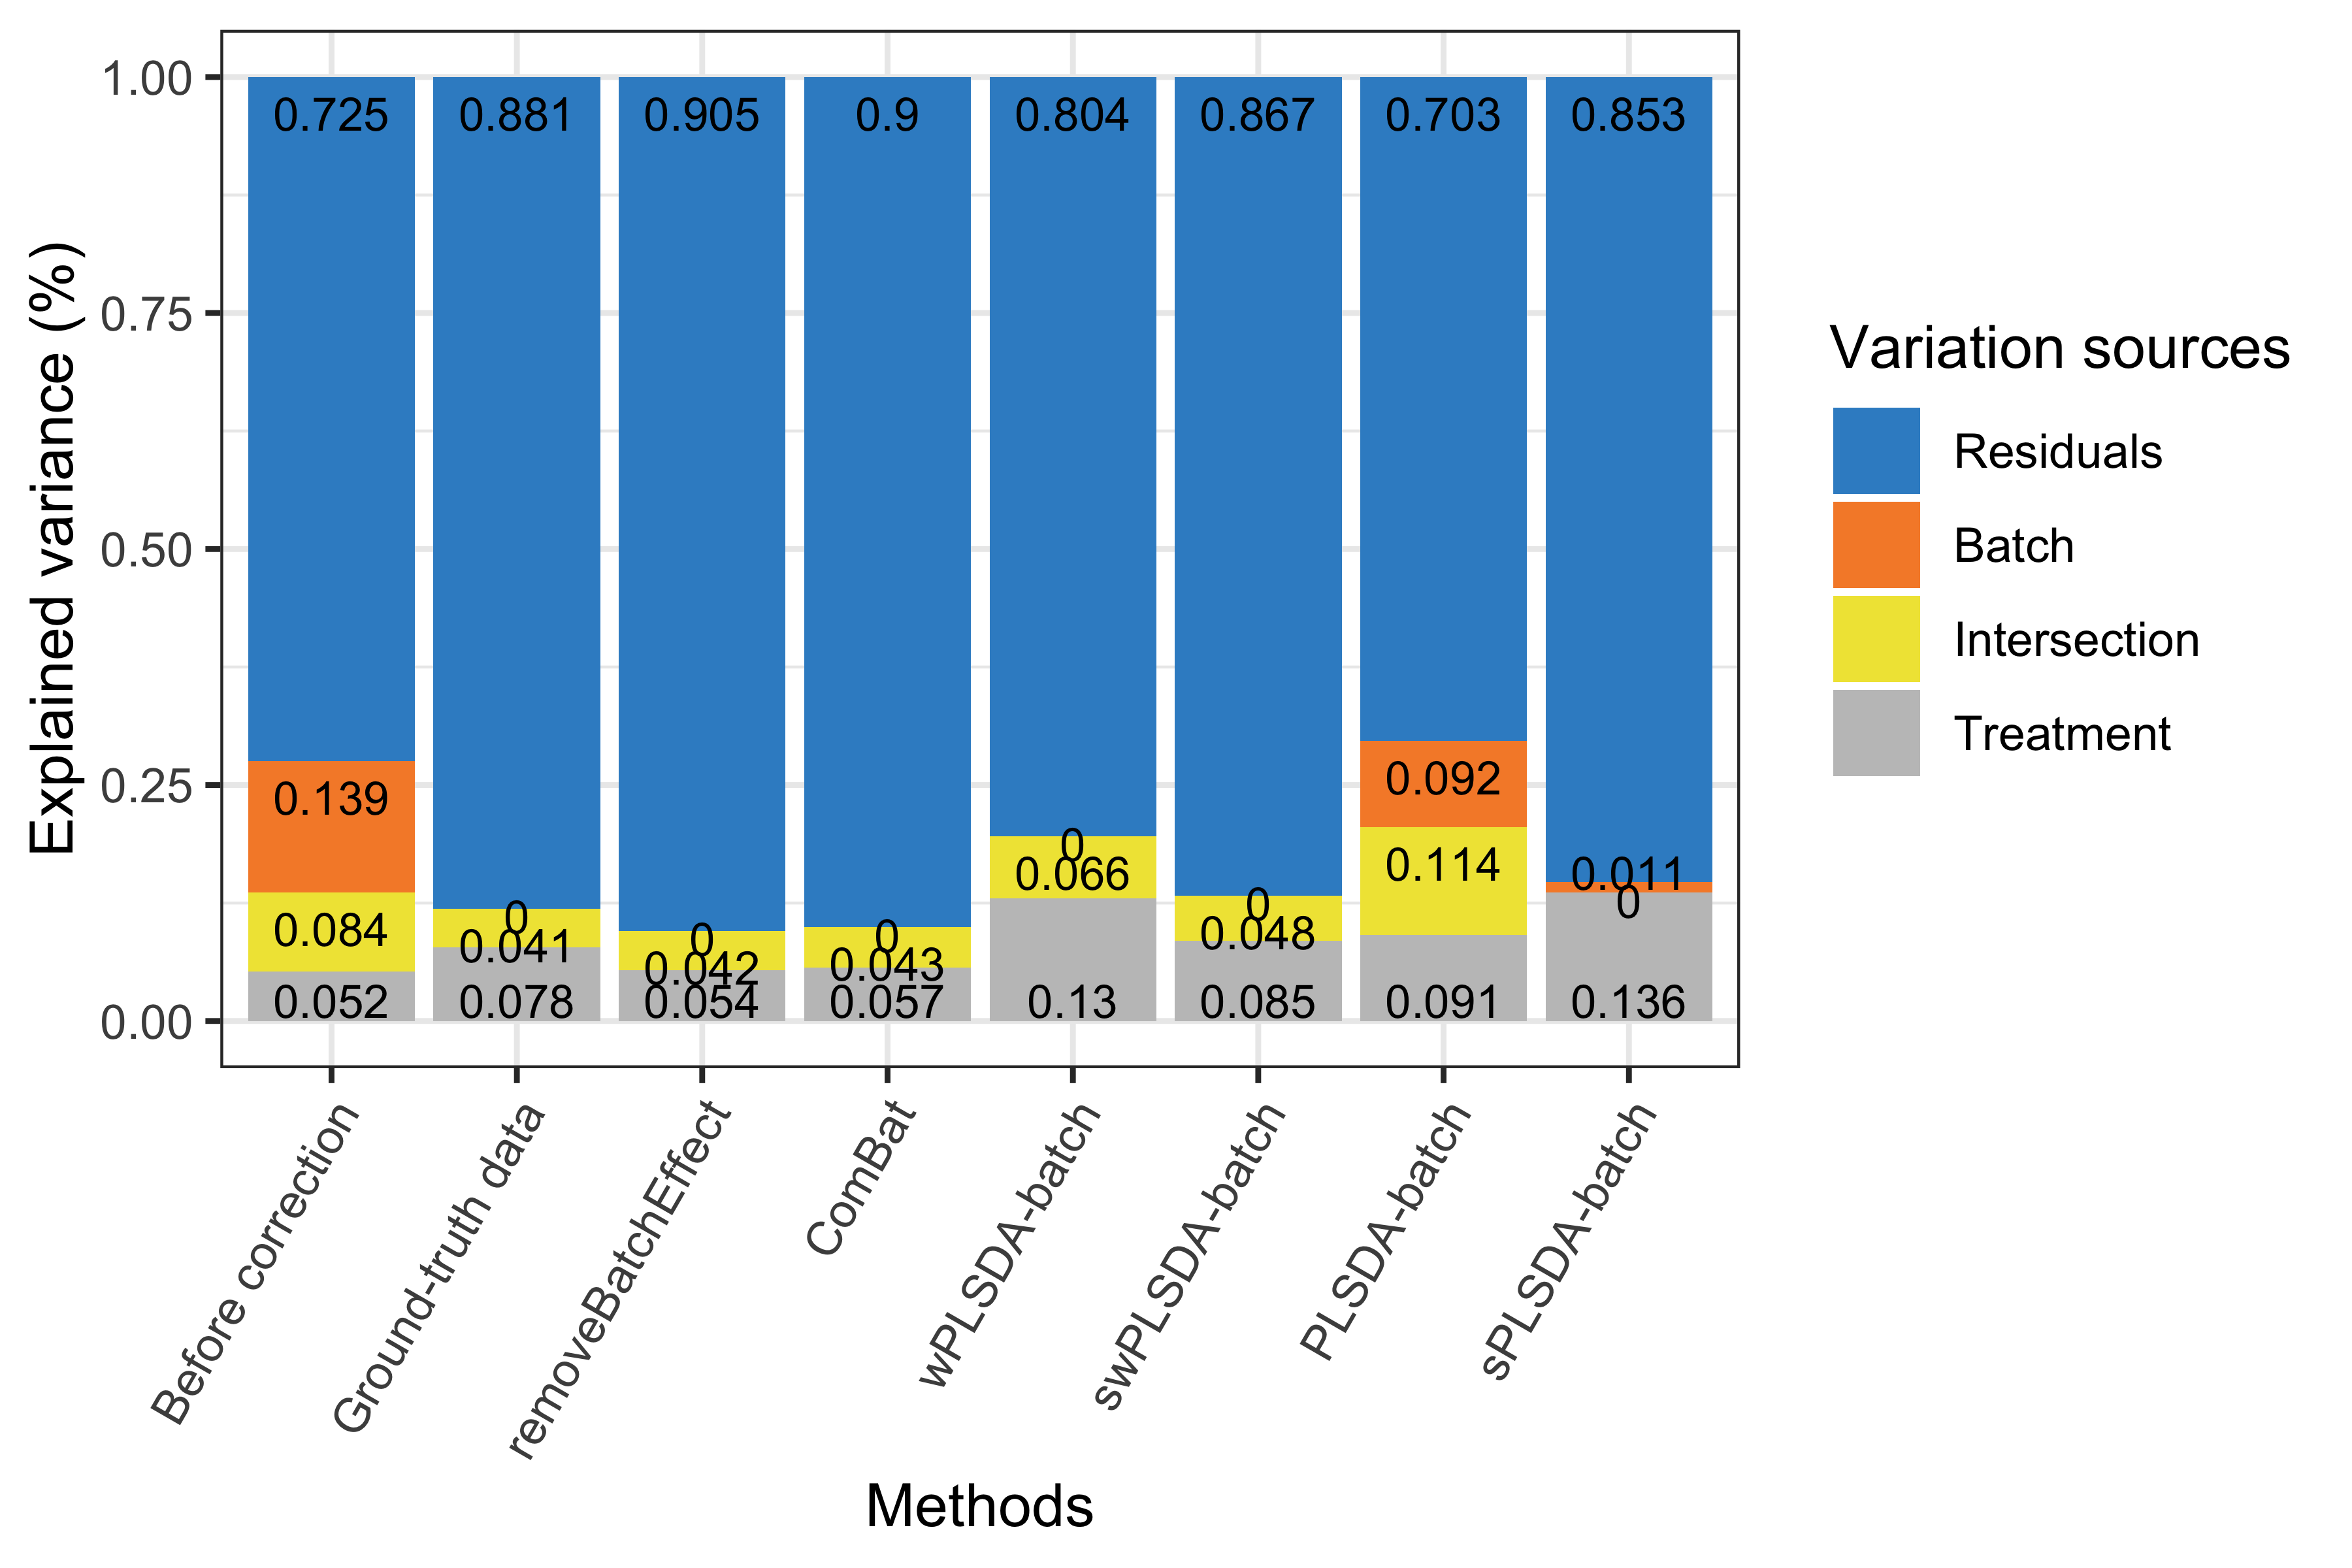
\includegraphics[width=0.6\linewidth]{PLSDAbatch_workflow_files/figure-latex/unnamed-chunk-105-1} 

}

\caption{Figure 3: Simulation studies (Gaussian distribution): comparison of explained variance before and after batch effect correction for the unbalanced batch × treatment design.}\label{fig:unnamed-chunk-105}
\end{figure}

With an unbalanced batch \(\times\) treatment design, we observed that certain amount of variance was shared (intersection) and explained by both batch and treatment effects. Such intersectional variance should exist even in the ground-truth data with no batch effect, as it originates from treatment variation because of the unbalanced design. Unweighted PLSDA-batch and sPLSDA-batch failed in such design, as their corrected data still included a large amount of batch variation (PLSDA-batch) or not included intersectional variance (sPLSDA-batch), while the other methods removed batch variation successfully. The corrected data from removeBatchEffect and ComBat included less proportion of variance explained by treatment but more intersectional variance compared to the ground-truth data. Although wPLSDA-batch corrected data included the largest treatment variance, swPLSDA-batch outperformed all methods with results similar to the ground-truth data.

\begin{Shaded}
\begin{Highlighting}[]
\DocumentationTok{\#\#\#\#\#\#\#\#\#\#\#\#\#\#\#\#\#\#\#\#\#\#\#\#\#\#\#\#\#\#\#\#\#\#\#\#\#\#\#\#\#\#\#\#\#\#\#\#\#\#\#\#\#\#\#\#\#\#\#\#\#\#\#\#\#\#\#\#\#\#\#\#\#\#\#\#\#\#\#\#}
\CommentTok{\# individual variance (R2)}
\CommentTok{\# color}
\NormalTok{gcolor }\OtherTok{\textless{}{-}} \FunctionTok{c}\NormalTok{(}\FunctionTok{rep}\NormalTok{(}\FunctionTok{pb\_color}\NormalTok{(}\DecValTok{16}\NormalTok{), p\_trt\_relevant), }
            \FunctionTok{rep}\NormalTok{(}\FunctionTok{pb\_color}\NormalTok{(}\DecValTok{17}\NormalTok{), (p\_total }\SpecialCharTok{{-}}\NormalTok{ p\_trt\_relevant)))}
\NormalTok{gcolor[}\FunctionTok{intersect}\NormalTok{(true.trt, true.batch)] }\OtherTok{=} \FunctionTok{pb\_color}\NormalTok{(}\DecValTok{18}\NormalTok{)}
\NormalTok{gcolor[}\FunctionTok{setdiff}\NormalTok{(}\FunctionTok{seq\_len}\NormalTok{(p\_total), }\FunctionTok{union}\NormalTok{(true.trt, true.batch))] }\OtherTok{=} \FunctionTok{pb\_color}\NormalTok{(}\DecValTok{15}\NormalTok{)}

\NormalTok{xlabs }\OtherTok{=} \StringTok{\textquotesingle{}R2(variable, treatment)\textquotesingle{}}
\NormalTok{ylabs }\OtherTok{=} \StringTok{\textquotesingle{}R2(variable, batch)\textquotesingle{}}
\NormalTok{edgex }\OtherTok{=} \FloatTok{0.7}
\NormalTok{edgey }\OtherTok{=} \FloatTok{0.6}

\CommentTok{\# scatterplot}
\FunctionTok{par}\NormalTok{(}\AttributeTok{mfrow =} \FunctionTok{c}\NormalTok{(}\DecValTok{3}\NormalTok{,}\DecValTok{2}\NormalTok{))}
\FunctionTok{plot}\NormalTok{(}\FunctionTok{rowMeans}\NormalTok{(r2.trt.before), }\FunctionTok{rowMeans}\NormalTok{(r2.batch.before), }\AttributeTok{col =}\NormalTok{ gcolor, }
     \AttributeTok{xlab =}\NormalTok{ xlabs, }\AttributeTok{ylab =}\NormalTok{ ylabs, }\AttributeTok{pch =} \FunctionTok{as.numeric}\NormalTok{(}\FunctionTok{as.factor}\NormalTok{(gcolor)),}
     \AttributeTok{xlim =} \FunctionTok{c}\NormalTok{(}\DecValTok{0}\NormalTok{, edgex), }\AttributeTok{ylim =} \FunctionTok{c}\NormalTok{(}\DecValTok{0}\NormalTok{, edgey), }
     \AttributeTok{main =} \StringTok{\textquotesingle{}Before correction\textquotesingle{}}\NormalTok{, }\AttributeTok{cex =} \FloatTok{0.7}\NormalTok{)}
\FunctionTok{legend}\NormalTok{(}\StringTok{\textquotesingle{}topright\textquotesingle{}}\NormalTok{, }\AttributeTok{legend =} \FunctionTok{c}\NormalTok{(}\StringTok{\textquotesingle{}No effect\textquotesingle{}}\NormalTok{, }\StringTok{\textquotesingle{}Treatment only\textquotesingle{}}\NormalTok{, }
                              \StringTok{\textquotesingle{}Batch only\textquotesingle{}}\NormalTok{, }\StringTok{\textquotesingle{}Treatment \& batch\textquotesingle{}}\NormalTok{), }
       \AttributeTok{col =} \FunctionTok{pb\_color}\NormalTok{(}\DecValTok{15}\SpecialCharTok{:}\DecValTok{18}\NormalTok{), }\AttributeTok{pch =} \FunctionTok{seq\_len}\NormalTok{(}\DecValTok{4}\NormalTok{), }\AttributeTok{cex =} \FloatTok{0.8}\NormalTok{)}

\FunctionTok{plot}\NormalTok{(}\FunctionTok{rowMeans}\NormalTok{(r2.trt.clean), }\FunctionTok{rowMeans}\NormalTok{(r2.batch.clean), }\AttributeTok{col =}\NormalTok{ gcolor, }
     \AttributeTok{xlab =}\NormalTok{ xlabs, }\AttributeTok{ylab =}\NormalTok{ ylabs, }\AttributeTok{pch =} \FunctionTok{as.numeric}\NormalTok{(}\FunctionTok{as.factor}\NormalTok{(gcolor)),}
     \AttributeTok{xlim =} \FunctionTok{c}\NormalTok{(}\DecValTok{0}\NormalTok{, edgex), }\AttributeTok{ylim =} \FunctionTok{c}\NormalTok{(}\DecValTok{0}\NormalTok{, edgey), }
     \AttributeTok{main =} \StringTok{\textquotesingle{}Ground{-}truth data\textquotesingle{}}\NormalTok{, }\AttributeTok{cex =} \FloatTok{0.7}\NormalTok{)}
\FunctionTok{legend}\NormalTok{(}\StringTok{\textquotesingle{}topright\textquotesingle{}}\NormalTok{, }\AttributeTok{legend =} \FunctionTok{c}\NormalTok{(}\StringTok{\textquotesingle{}No effect\textquotesingle{}}\NormalTok{, }\StringTok{\textquotesingle{}Treatment only\textquotesingle{}}\NormalTok{, }
                              \StringTok{\textquotesingle{}Batch only\textquotesingle{}}\NormalTok{, }\StringTok{\textquotesingle{}Treatment \& batch\textquotesingle{}}\NormalTok{), }
       \AttributeTok{col =} \FunctionTok{pb\_color}\NormalTok{(}\DecValTok{15}\SpecialCharTok{:}\DecValTok{18}\NormalTok{), }\AttributeTok{pch =} \FunctionTok{seq\_len}\NormalTok{(}\DecValTok{4}\NormalTok{), }\AttributeTok{cex =} \FloatTok{0.8}\NormalTok{)}

\FunctionTok{plot}\NormalTok{(}\FunctionTok{rowMeans}\NormalTok{(r2.trt.rbe), }\FunctionTok{rowMeans}\NormalTok{(r2.batch.rbe), }\AttributeTok{col =}\NormalTok{ gcolor, }
     \AttributeTok{xlab =}\NormalTok{ xlabs, }\AttributeTok{ylab =}\NormalTok{ ylabs, }\AttributeTok{pch =} \FunctionTok{as.numeric}\NormalTok{(}\FunctionTok{as.factor}\NormalTok{(gcolor)),}
     \AttributeTok{xlim =} \FunctionTok{c}\NormalTok{(}\DecValTok{0}\NormalTok{, edgex), }\AttributeTok{ylim =} \FunctionTok{c}\NormalTok{(}\DecValTok{0}\NormalTok{, edgey), }
     \AttributeTok{main =} \StringTok{\textquotesingle{}removeBatchEffect\textquotesingle{}}\NormalTok{, }\AttributeTok{cex =} \FloatTok{0.7}\NormalTok{)}
\FunctionTok{legend}\NormalTok{(}\StringTok{\textquotesingle{}topright\textquotesingle{}}\NormalTok{, }\AttributeTok{legend =} \FunctionTok{c}\NormalTok{(}\StringTok{\textquotesingle{}No effect\textquotesingle{}}\NormalTok{, }\StringTok{\textquotesingle{}Treatment only\textquotesingle{}}\NormalTok{, }
                              \StringTok{\textquotesingle{}Batch only\textquotesingle{}}\NormalTok{, }\StringTok{\textquotesingle{}Treatment \& batch\textquotesingle{}}\NormalTok{), }
       \AttributeTok{col =} \FunctionTok{pb\_color}\NormalTok{(}\DecValTok{15}\SpecialCharTok{:}\DecValTok{18}\NormalTok{), }\AttributeTok{pch =} \FunctionTok{seq\_len}\NormalTok{(}\DecValTok{4}\NormalTok{), }\AttributeTok{cex =} \FloatTok{0.8}\NormalTok{)}

\FunctionTok{plot}\NormalTok{(}\FunctionTok{rowMeans}\NormalTok{(r2.trt.combat), }\FunctionTok{rowMeans}\NormalTok{(r2.batch.combat), }\AttributeTok{col =}\NormalTok{ gcolor, }
     \AttributeTok{xlab =}\NormalTok{ xlabs, }\AttributeTok{ylab =}\NormalTok{ ylabs, }\AttributeTok{pch =} \FunctionTok{as.numeric}\NormalTok{(}\FunctionTok{as.factor}\NormalTok{(gcolor)),}
     \AttributeTok{xlim =} \FunctionTok{c}\NormalTok{(}\DecValTok{0}\NormalTok{, edgex), }\AttributeTok{ylim =} \FunctionTok{c}\NormalTok{(}\DecValTok{0}\NormalTok{, edgey), }\AttributeTok{main =} \StringTok{\textquotesingle{}ComBat\textquotesingle{}}\NormalTok{, }\AttributeTok{cex =} \FloatTok{0.7}\NormalTok{)}
\FunctionTok{legend}\NormalTok{(}\StringTok{\textquotesingle{}topright\textquotesingle{}}\NormalTok{, }\AttributeTok{legend =} \FunctionTok{c}\NormalTok{(}\StringTok{\textquotesingle{}No effect\textquotesingle{}}\NormalTok{, }\StringTok{\textquotesingle{}Treatment only\textquotesingle{}}\NormalTok{, }
                              \StringTok{\textquotesingle{}Batch only\textquotesingle{}}\NormalTok{, }\StringTok{\textquotesingle{}Treatment \& batch\textquotesingle{}}\NormalTok{), }
       \AttributeTok{col =} \FunctionTok{pb\_color}\NormalTok{(}\DecValTok{15}\SpecialCharTok{:}\DecValTok{18}\NormalTok{), }\AttributeTok{pch =} \FunctionTok{seq\_len}\NormalTok{(}\DecValTok{4}\NormalTok{), }\AttributeTok{cex =} \FloatTok{0.8}\NormalTok{)}

\FunctionTok{plot}\NormalTok{(}\FunctionTok{rowMeans}\NormalTok{(r2.trt.wplsdab), }\FunctionTok{rowMeans}\NormalTok{(r2.batch.wplsdab), }\AttributeTok{col =}\NormalTok{ gcolor, }
     \AttributeTok{xlab =}\NormalTok{ xlabs, }\AttributeTok{ylab =}\NormalTok{ ylabs, }\AttributeTok{pch =} \FunctionTok{as.numeric}\NormalTok{(}\FunctionTok{as.factor}\NormalTok{(gcolor)),}
     \AttributeTok{xlim =} \FunctionTok{c}\NormalTok{(}\DecValTok{0}\NormalTok{, edgex), }\AttributeTok{ylim =} \FunctionTok{c}\NormalTok{(}\DecValTok{0}\NormalTok{, edgey), }\AttributeTok{main =} \StringTok{\textquotesingle{}wPLSDA{-}batch\textquotesingle{}}\NormalTok{, }\AttributeTok{cex =} \FloatTok{0.7}\NormalTok{)}
\FunctionTok{legend}\NormalTok{(}\StringTok{\textquotesingle{}topright\textquotesingle{}}\NormalTok{, }\AttributeTok{legend =} \FunctionTok{c}\NormalTok{(}\StringTok{\textquotesingle{}No effect\textquotesingle{}}\NormalTok{, }\StringTok{\textquotesingle{}Treatment only\textquotesingle{}}\NormalTok{, }
                              \StringTok{\textquotesingle{}Batch only\textquotesingle{}}\NormalTok{, }\StringTok{\textquotesingle{}Treatment \& batch\textquotesingle{}}\NormalTok{), }
       \AttributeTok{col =} \FunctionTok{pb\_color}\NormalTok{(}\DecValTok{15}\SpecialCharTok{:}\DecValTok{18}\NormalTok{), }\AttributeTok{pch =} \FunctionTok{seq\_len}\NormalTok{(}\DecValTok{4}\NormalTok{), }\AttributeTok{cex =} \FloatTok{0.8}\NormalTok{)}

\FunctionTok{plot}\NormalTok{(}\FunctionTok{rowMeans}\NormalTok{(r2.trt.swplsdab), }\FunctionTok{rowMeans}\NormalTok{(r2.batch.swplsdab), }\AttributeTok{col =}\NormalTok{ gcolor, }
     \AttributeTok{xlab =}\NormalTok{ xlabs, }\AttributeTok{ylab =}\NormalTok{ ylabs, }\AttributeTok{pch =} \FunctionTok{as.numeric}\NormalTok{(}\FunctionTok{as.factor}\NormalTok{(gcolor)),}
     \AttributeTok{xlim =} \FunctionTok{c}\NormalTok{(}\DecValTok{0}\NormalTok{, edgex), }\AttributeTok{ylim =} \FunctionTok{c}\NormalTok{(}\DecValTok{0}\NormalTok{, edgey), }\AttributeTok{main =} \StringTok{\textquotesingle{}swPLSDA{-}batch\textquotesingle{}}\NormalTok{, }\AttributeTok{cex =} \FloatTok{0.7}\NormalTok{)}
\FunctionTok{legend}\NormalTok{(}\StringTok{\textquotesingle{}topright\textquotesingle{}}\NormalTok{, }\AttributeTok{legend =} \FunctionTok{c}\NormalTok{(}\StringTok{\textquotesingle{}No effect\textquotesingle{}}\NormalTok{, }\StringTok{\textquotesingle{}Treatment only\textquotesingle{}}\NormalTok{, }
                              \StringTok{\textquotesingle{}Batch only\textquotesingle{}}\NormalTok{, }\StringTok{\textquotesingle{}Treatment \& batch\textquotesingle{}}\NormalTok{), }
       \AttributeTok{col =} \FunctionTok{pb\_color}\NormalTok{(}\DecValTok{15}\SpecialCharTok{:}\DecValTok{18}\NormalTok{), }\AttributeTok{pch =} \FunctionTok{seq\_len}\NormalTok{(}\DecValTok{4}\NormalTok{), }\AttributeTok{cex =} \FloatTok{0.8}\NormalTok{)}
\end{Highlighting}
\end{Shaded}

\begin{figure}

{\centering 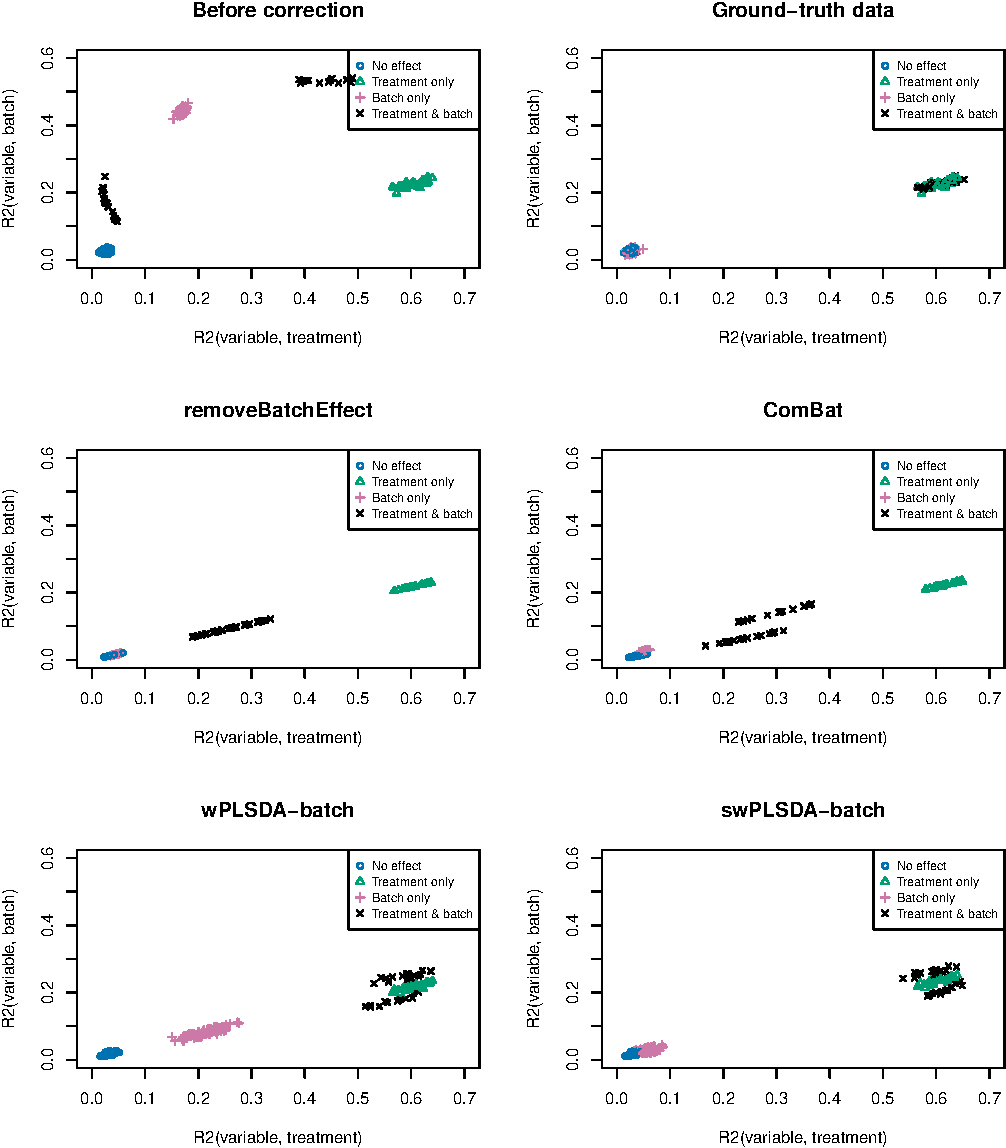
\includegraphics[width=1\linewidth]{PLSDAbatch_workflow_files/figure-latex/unnamed-chunk-106-1} 

}

\caption{Figure 4: Simulation studies (Gaussian distribution): R2 values for each microbial variable before and after batch effect correction for the unbalanced batch × treatment design.}\label{fig:unnamed-chunk-106}
\end{figure}

\begin{Shaded}
\begin{Highlighting}[]
\FunctionTok{par}\NormalTok{(}\AttributeTok{mfrow =} \FunctionTok{c}\NormalTok{(}\DecValTok{1}\NormalTok{,}\DecValTok{1}\NormalTok{))}
\end{Highlighting}
\end{Shaded}

Based on the \(R^2\) values, variables assigned with both treatment and batch effects were segregated into two groups depending on whether their abundance increased or decreased consistently or not according to the two effects. We observed similar results to those obtained from the balanced design.

\begin{Shaded}
\begin{Highlighting}[]
\CommentTok{\# precision \& recall \& F1 (ANOVA \& sPLSDA)}
\DocumentationTok{\#\# mean}
\NormalTok{acc\_mean }\OtherTok{\textless{}{-}} \FunctionTok{rbind}\NormalTok{(}\FunctionTok{colMeans}\NormalTok{(precision\_limma), }\FunctionTok{colMeans}\NormalTok{(recall\_limma), }
                  \FunctionTok{colMeans}\NormalTok{(F1\_limma), }\FunctionTok{colMeans}\NormalTok{(precision\_splsda))}
\FunctionTok{rownames}\NormalTok{(acc\_mean) }\OtherTok{\textless{}{-}} \FunctionTok{c}\NormalTok{(}\StringTok{\textquotesingle{}Precision\textquotesingle{}}\NormalTok{, }\StringTok{\textquotesingle{}Recall\textquotesingle{}}\NormalTok{, }\StringTok{\textquotesingle{}F1\textquotesingle{}}\NormalTok{, }\StringTok{\textquotesingle{}Multivariate selection\textquotesingle{}}\NormalTok{)}
\FunctionTok{colnames}\NormalTok{(acc\_mean) }\OtherTok{\textless{}{-}} \FunctionTok{c}\NormalTok{(}\StringTok{\textquotesingle{}Before correction\textquotesingle{}}\NormalTok{, }\StringTok{\textquotesingle{}Ground{-}truth data\textquotesingle{}}\NormalTok{, }
                        \StringTok{\textquotesingle{}removeBatchEffect\textquotesingle{}}\NormalTok{, }\StringTok{\textquotesingle{}ComBat\textquotesingle{}}\NormalTok{, }
                        \StringTok{\textquotesingle{}wPLSDA{-}batch\textquotesingle{}}\NormalTok{, }\StringTok{\textquotesingle{}swPLSDA{-}batch\textquotesingle{}}\NormalTok{)}
\NormalTok{acc\_mean }\OtherTok{\textless{}{-}} \FunctionTok{format}\NormalTok{(acc\_mean, }\AttributeTok{digits =} \DecValTok{2}\NormalTok{)}
\NormalTok{knitr}\SpecialCharTok{::}\FunctionTok{kable}\NormalTok{(acc\_mean, }\AttributeTok{caption =} \StringTok{\textquotesingle{}Table 6: Simulation studies (Gaussian distribution): summary of accuracy measures before and after batch correction for the unbalanced batch × treatment design (mean).\textquotesingle{}}\NormalTok{)}
\end{Highlighting}
\end{Shaded}

\begin{table}

\caption{\label{tab:unnamed-chunk-107}Table 6: Simulation studies (Gaussian distribution): summary of accuracy measures before and after batch correction for the unbalanced batch × treatment design (mean).}
\centering
\begin{tabular}[t]{l|l|l|l|l|l|l}
\hline
  & Before correction & Ground-truth data & removeBatchEffect & ComBat & wPLSDA-batch & swPLSDA-batch\\
\hline
Precision & 0.52 & 0.96 & 0.85 & 0.80 & 0.52 & 0.80\\
\hline
Recall & 0.72 & 1.00 & 0.86 & 0.86 & 0.99 & 1.00\\
\hline
F1 & 0.55 & 0.98 & 0.84 & 0.81 & 0.65 & 0.88\\
\hline
Multivariate selection & 0.73 & 1.00 & 0.88 & 0.87 & 0.89 & 0.99\\
\hline
\end{tabular}
\end{table}

When considering the measures of accuracy with univariate one-way ANOVA, we observed that the corrected data from wPLSDA-batch and swPLSDA-batch led to higher recall and lower precision than the data from removeBatchEffect and ComBat. However, the precision of swPLSDA-batch was competitive to removeBatchEffect and ComBat. Moreover, weighted sPLSDA-batch achieved higher F1 scores and multivariate selection scores than removeBatchEffect and ComBat.

\begin{Shaded}
\begin{Highlighting}[]
\DocumentationTok{\#\# sd}
\NormalTok{acc\_sd }\OtherTok{\textless{}{-}} \FunctionTok{rbind}\NormalTok{(}\FunctionTok{apply}\NormalTok{(precision\_limma, }\DecValTok{2}\NormalTok{, sd), }\FunctionTok{apply}\NormalTok{(recall\_limma, }\DecValTok{2}\NormalTok{, sd), }
                \FunctionTok{apply}\NormalTok{(F1\_limma, }\DecValTok{2}\NormalTok{, sd), }\FunctionTok{apply}\NormalTok{(precision\_splsda, }\DecValTok{2}\NormalTok{, sd))}
\FunctionTok{rownames}\NormalTok{(acc\_sd) }\OtherTok{\textless{}{-}} \FunctionTok{c}\NormalTok{(}\StringTok{\textquotesingle{}Precision\textquotesingle{}}\NormalTok{, }\StringTok{\textquotesingle{}Recall\textquotesingle{}}\NormalTok{, }\StringTok{\textquotesingle{}F1\textquotesingle{}}\NormalTok{, }\StringTok{\textquotesingle{}Multivariate selection\textquotesingle{}}\NormalTok{)}
\FunctionTok{colnames}\NormalTok{(acc\_sd) }\OtherTok{\textless{}{-}} \FunctionTok{c}\NormalTok{(}\StringTok{\textquotesingle{}Before correction\textquotesingle{}}\NormalTok{, }\StringTok{\textquotesingle{}Ground{-}truth data\textquotesingle{}}\NormalTok{, }
                      \StringTok{\textquotesingle{}removeBatchEffect\textquotesingle{}}\NormalTok{, }\StringTok{\textquotesingle{}ComBat\textquotesingle{}}\NormalTok{, }
                      \StringTok{\textquotesingle{}wPLSDA{-}batch\textquotesingle{}}\NormalTok{, }\StringTok{\textquotesingle{}swPLSDA{-}batch\textquotesingle{}}\NormalTok{)}
\NormalTok{acc\_sd }\OtherTok{\textless{}{-}} \FunctionTok{format}\NormalTok{(acc\_sd, }\AttributeTok{digits =} \DecValTok{2}\NormalTok{)}
\NormalTok{knitr}\SpecialCharTok{::}\FunctionTok{kable}\NormalTok{(acc\_sd, }\AttributeTok{caption =} \StringTok{\textquotesingle{}Table 7: Simulation studies (Gaussian distribution): summary of accuracy measures before and after batch correction for the unbalanced batch × treatment design (standard deviation).\textquotesingle{}}\NormalTok{)}
\end{Highlighting}
\end{Shaded}

\begin{table}

\caption{\label{tab:unnamed-chunk-108}Table 7: Simulation studies (Gaussian distribution): summary of accuracy measures before and after batch correction for the unbalanced batch × treatment design (standard deviation).}
\centering
\begin{tabular}[t]{l|l|l|l|l|l|l}
\hline
  & Before correction & Ground-truth data & removeBatchEffect & ComBat & wPLSDA-batch & swPLSDA-batch\\
\hline
Precision & 0.325 & 0.031 & 0.176 & 0.231 & 0.232 & 0.137\\
\hline
Recall & 0.042 & 0.000 & 0.104 & 0.100 & 0.029 & 0.000\\
\hline
F1 & 0.212 & 0.017 & 0.137 & 0.177 & 0.189 & 0.092\\
\hline
Multivariate selection & 0.051 & 0.000 & 0.069 & 0.083 & 0.148 & 0.016\\
\hline
\end{tabular}
\end{table}

The standard deviations of the multivariate selection scores were all smaller than the univariate selection scores for the different corrected data, indicating a better stability of the variables selected by multivariate sPLSDA compared to the one-way ANOVA univariate selection.

\hypertarget{references-2}{%
\section{References}\label{references-2}}

\hypertarget{batch-effects-management-in-simulation-studies-negative-binomial-distribution}{%
\chapter{Batch Effects Management in Simulation Studies (Negative Binomial Distribution)}\label{batch-effects-management-in-simulation-studies-negative-binomial-distribution}}

\hypertarget{introduction-2}{%
\section{Introduction}\label{introduction-2}}

Microbiome data are multivariate with inherent correlation structure between microbial variables. The data are over-dispersed with a distribution close to a negative binomial distribution \citep{mcmurdie2014waste, quinn2018understanding}. Inspired by \citep{hawinkel2019broken}, we simulated data from multivariate negative binomial distribution achieved with quantile-quantile transformation between multivariate normal and negative binomial distributions. To add treatment and batch effects, we used matrix factorisation to simulate the mean for modelling negative binomial distribution as a matrix \[\Theta = \begin{bmatrix}
\theta_{11} & ...  & \theta_{1M}\\
...& ... & ... \\
\theta_{1N} & ... & \theta_{NM}
\end{bmatrix}\] for \(N\) samples and \(M\) microbial variables as follows:

\[\Theta = exp(x_{(trt)}^{\top}\beta^{(trt)} + x_{(batch)}^{\top}\beta^{(batch)} + \epsilon)\]

\noindent where \(x_{(trt)}\) and \(x_{(batch)}\) represent the design vectors of treatment and batch effects respectively for each sample. \(\beta^{(trt)}\) and \(\beta^{(batch)}\) represent the regression coefficients of treatment and batch effects for each microbial variable, and \(\beta^{(trt)}_{j} \in N(\mu_{(trt)},\sigma_{(trt)}^{2})\), \(\beta^{(batch)}_{j} \in N(\mu_{(batch)},\sigma_{(batch)}^{2})\). \(\epsilon\) contains the random noise that is independent and identically distributed (i.i.d) and \(\epsilon_{ij} \in N(0,\delta^{2})\), in which \(i = 1,2,...,N\) samples, \(j = 1,2,..,M\) variables.

The probability matrix \[P = \begin{bmatrix}
p_{11} & ...  & p_{1M}\\
...& ... & ... \\
p_{1N} & ... & p_{NM}
\end{bmatrix}\] for modelling negative binomial distribution is calculated as

\[p_{ij} = \frac{r}{r + \theta_{ij}}\]
\noindent where \(p_{ij}\) and \(\theta_{ij}\) represent the probability of success in each trial and the mean for negative binomial distribution of sample \(i\) and microbial variable \(j\), and \(r\) is the dispersion parameter representing the number of successes.

We then simulated a data matrix based on multivariate normal distribution with mean \(0\) and correlation matrix \(\Sigma\):

\[X^{normal} = N(0, \Sigma)\]

\noindent where the correlation matrix \(\Sigma\) was simulated with the strategy adapted from \citep{mcgregor2020mdine} as follows: We first generated a lower-triangular matrix \(L\), in which the diagonal elements follow \(Unif(1.5, 2.5)\), and the other elements \(Unif(-1.5, 1.5)\). We randomly set the elements outside the diagonal of \(L\) to zero with probability \(0.7\). A precision matrix, which is the inverse of covariance matrix was created as \(R^{-1} = LL^{\top}\). The corresponding correlation matrix \(\Sigma\) to \(R\) was then obtained. These parameters were set according to \citep{mcgregor2020mdine}.

Thereafter we used Cumulative Distribution Function (CDF) to achieve quantile-quantile transformation as:

\[CDF(x^{normal}_{ij}) = CDF(x^{nb}_{ij})\]

\noindent where \(CDF(x^{normal}_{ij})\) represents the cumulative probability of \(x^{normal}_{ij}\) for sample \(i\) and variable \(j\) that belongs to matrix \(X^{normal}\) from multivariate normal distribution. \(CDF(x^{nb}_{ij})\) represents the cumulative probability of each \(x^{nb}_{ij}\) in matrix \(X^{nb}\) from negative binomial distribution.

Based on the cumulative probability, we can simulate a data matrix \(X^{nb}\) with multivariate negative binomial distribution:

\[X^{nb} = NB(r, P, \Sigma)\]

\noindent where \(r\) represents the dispersion parameter, \(P\) represents the probability matrix and \(\Sigma\) the correlation matrix explaining the dependence structure between microbial variables.

We simulated datasets with different parameters including amount of batch and treatment effects (\(\mu_{(batch)}\), \(\mu_{(trt)}\)) and variability among variables (\(\sigma_{(batch)}\), \(\sigma_{(trt)}\)), number of variables with batch and/or treatment effects (\(M^{(batch)}\), \(M^{(trt)}\) and \(M^{(trt \ \& \ batch)}\)), balanced and unbalanced batch \(\times\) treatment designs, as summarised in the table below.

\textbf{Table 1: Summary of simulation scenarios (Negative Binomial distribution).} For a given choice of parameters reported in this table, each simulation was repeated 50 times. \(M^{(trt)}, M^{(batch)}\) and \(M^{(trt \ \& \ batch)}\) represent the number of variables with treatment, batch, or both effects respectively. Simu 6 includes parameters likely to represent real data according to our experience in analysing microbiome datasets.

\small

\begin{longtable}[]{@{}
  >{\centering\arraybackslash}p{(\columnwidth - 14\tabcolsep) * \real{0.0845}}
  >{\centering\arraybackslash}p{(\columnwidth - 14\tabcolsep) * \real{0.1056}}
  >{\centering\arraybackslash}p{(\columnwidth - 14\tabcolsep) * \real{0.1268}}
  >{\centering\arraybackslash}p{(\columnwidth - 14\tabcolsep) * \real{0.1197}}
  >{\centering\arraybackslash}p{(\columnwidth - 14\tabcolsep) * \real{0.1408}}
  >{\centering\arraybackslash}p{(\columnwidth - 14\tabcolsep) * \real{0.1197}}
  >{\centering\arraybackslash}p{(\columnwidth - 14\tabcolsep) * \real{0.1197}}
  >{\centering\arraybackslash}p{(\columnwidth - 14\tabcolsep) * \real{0.1831}}@{}}
\toprule()
\begin{minipage}[b]{\linewidth}\centering
\end{minipage} & \begin{minipage}[b]{\linewidth}\centering
\(\mu_{(trt)}\)
\end{minipage} & \begin{minipage}[b]{\linewidth}\centering
\(\sigma_{(trt)}\)
\end{minipage} & \begin{minipage}[b]{\linewidth}\centering
\(\mu_{(batch)}\)
\end{minipage} & \begin{minipage}[b]{\linewidth}\centering
\(\sigma_{(batch)}\)
\end{minipage} & \begin{minipage}[b]{\linewidth}\centering
\(M^{(trt)}\)
\end{minipage} & \begin{minipage}[b]{\linewidth}\centering
\(M^{(batch)}\)
\end{minipage} & \begin{minipage}[b]{\linewidth}\centering
\(M^{(trt \ \& \ batch)}\)
\end{minipage} \\
\midrule()
\endhead
Simu 1 & 3 & 1 & 7 & \{1,4,8\} & 60 & 150 & 0 \\
Simu 2 & \{3,5,7\} & 1 & 7 & 8 & 60 & 150 & 0 \\
Simu 3 & 3 & \{1,2,4\} & 7 & 8 & 60 & 150 & 0 \\
Simu 4 & 3 & 2 & 7 & 8 & \{30,60,100,150\} & 150 & 0 \\
Simu 5 & 3 & 2 & 7 & 8 & 60 & \{30,60,100,150\} & 0 \\
Simu 6 & 3 & 2 & 7 & 8 & 60 & 150 & \{0,18,30,42,60\} \\
\bottomrule()
\end{longtable}

\normalsize

The microbial variables with treatment or batch effects were randomly indexed in the data with non-zero \(\beta^{(trt)}\) or \(\beta^{(batch)}\). The background noise \(\epsilon_{ij}\) was randomly sampled from \(N(0,0.2^{2})\), reflecting real microbiome datasets.

We also simulated datasets with different number of batch groups:

\begin{enumerate}
\def\labelenumi{\arabic{enumi}.}
\tightlist
\item
  Two batch groups: Each dataset included 300 variables and 40 samples grouped according to two treatments (trt1 and trt2) and two batches (batch1 and batch2).\\
\item
  Three batch groups: Each dataset included 300 variables and 36 samples grouped according to two treatments (trt1 and trt2) and three batches (batch1, batch2 and batch3).
\end{enumerate}

In addition, we simulated a ground-truth dataset that only included treatment effects and background noise without batch effects to evaluate batch effect correction methods.

Our simulations generate over-dispersed count data with batch and treatment effects as well as correlation structure among variables, but without any compositional structure. We therefore only applied natural log transformation to the simulated data prior to analysis.

In these simulation scenarios, for PLSDA-batch we set \(C-1\) (or \(B-1\)) components associated with treatment (or batch) effects (where \(C\) and \(B\) represent the total number of treatment and batch groups respectively) as \(C-1\) (\(B-1\)) components are likely to explain 100\% variance in \(Y\). The number of variables with a true treatment effect (\(M^{(trt)}\)) is set as the optimal number to select on each treatment component in sPLSDA-batch.

\hypertarget{simulations-two-batch-groups}{%
\section{Simulations (two batch groups)}\label{simulations-two-batch-groups}}

\hypertarget{balanced-batch-times-treatment-design-1}{%
\subsection{\texorpdfstring{Balanced batch \(\times\) treatment design}{Balanced batch \textbackslash times treatment design}}\label{balanced-batch-times-treatment-design-1}}

The balanced batch \(\times\) treatment experimental design included 10 samples from two batches respectively in each treatment group.

\textbf{Table 2: Balanced batch} \(\times\) treatment design in the simulation study

\begin{longtable}[]{@{}ccc@{}}
\toprule()
& Trt1 & Trt2 \\
\midrule()
\endhead
Batch1 & 10 & 10 \\
Batch2 & 10 & 10 \\
\bottomrule()
\end{longtable}

\begin{Shaded}
\begin{Highlighting}[]
\NormalTok{nitr }\OtherTok{\textless{}{-}} \DecValTok{50}
\NormalTok{N }\OtherTok{=} \DecValTok{40}
\NormalTok{p\_total }\OtherTok{=} \DecValTok{300}
\NormalTok{p\_trt\_relevant }\OtherTok{=} \DecValTok{100} 
\NormalTok{p\_bat\_relevant }\OtherTok{=} \DecValTok{200} 

\CommentTok{\# global variance (RDA)}
\NormalTok{gvar.before }\OtherTok{\textless{}{-}}\NormalTok{ gvar.clean }\OtherTok{\textless{}{-}} 
\NormalTok{  gvar.rbe }\OtherTok{\textless{}{-}}\NormalTok{ gvar.combat }\OtherTok{\textless{}{-}} 
\NormalTok{  gvar.plsdab }\OtherTok{\textless{}{-}}\NormalTok{ gvar.splsdab }\OtherTok{\textless{}{-}} \FunctionTok{data.frame}\NormalTok{(}\AttributeTok{treatment =} \ConstantTok{NA}\NormalTok{, }\AttributeTok{batch =} \ConstantTok{NA}\NormalTok{,  }
                                            \AttributeTok{intersection =} \ConstantTok{NA}\NormalTok{, }
                                            \AttributeTok{residual =} \ConstantTok{NA}\NormalTok{)}

\CommentTok{\# individual variance (R2)}
\NormalTok{r2.trt.before }\OtherTok{\textless{}{-}}\NormalTok{ r2.trt.clean }\OtherTok{\textless{}{-}} 
\NormalTok{  r2.trt.rbe  }\OtherTok{\textless{}{-}}\NormalTok{ r2.trt.combat }\OtherTok{\textless{}{-}} 
\NormalTok{  r2.trt.plsdab }\OtherTok{\textless{}{-}}\NormalTok{ r2.trt.splsdab }\OtherTok{\textless{}{-}} \FunctionTok{data.frame}\NormalTok{(}\FunctionTok{matrix}\NormalTok{(}\ConstantTok{NA}\NormalTok{, }\AttributeTok{nrow =}\NormalTok{ p\_total, }
                                                       \AttributeTok{ncol =}\NormalTok{ nitr))}
\NormalTok{r2.batch.before }\OtherTok{\textless{}{-}}\NormalTok{ r2.batch.clean }\OtherTok{\textless{}{-}} 
\NormalTok{  r2.batch.rbe  }\OtherTok{\textless{}{-}}\NormalTok{ r2.batch.combat }\OtherTok{\textless{}{-}} 
\NormalTok{  r2.batch.plsdab }\OtherTok{\textless{}{-}}\NormalTok{ r2.batch.splsdab }\OtherTok{\textless{}{-}} \FunctionTok{data.frame}\NormalTok{(}\FunctionTok{matrix}\NormalTok{(}\ConstantTok{NA}\NormalTok{, }\AttributeTok{nrow =}\NormalTok{ p\_total, }
                                                           \AttributeTok{ncol =}\NormalTok{ nitr))}

\CommentTok{\# precision \& recall \& F1 (ANOVA)}
\NormalTok{precision\_limma }\OtherTok{\textless{}{-}}\NormalTok{ recall\_limma }\OtherTok{\textless{}{-}}\NormalTok{ F1\_limma }\OtherTok{\textless{}{-}} 
  \FunctionTok{data.frame}\NormalTok{(}\AttributeTok{before =} \ConstantTok{NA}\NormalTok{, }\AttributeTok{clean =} \ConstantTok{NA}\NormalTok{, }
             \AttributeTok{rbe =} \ConstantTok{NA}\NormalTok{, }\AttributeTok{combat =} \ConstantTok{NA}\NormalTok{, }
             \AttributeTok{plsda\_batch =} \ConstantTok{NA}\NormalTok{, }\AttributeTok{splsda\_batch =} \ConstantTok{NA}\NormalTok{, }
             \AttributeTok{sva =} \ConstantTok{NA}\NormalTok{)}

\CommentTok{\# auc (splsda)}
\NormalTok{auc\_splsda }\OtherTok{\textless{}{-}} 
  \FunctionTok{data.frame}\NormalTok{(}\AttributeTok{before =} \ConstantTok{NA}\NormalTok{, }\AttributeTok{clean =} \ConstantTok{NA}\NormalTok{, }
             \AttributeTok{rbe =} \ConstantTok{NA}\NormalTok{, }\AttributeTok{combat =} \ConstantTok{NA}\NormalTok{, }
             \AttributeTok{plsda\_batch =} \ConstantTok{NA}\NormalTok{, }\AttributeTok{splsda\_batch =} \ConstantTok{NA}\NormalTok{)}


\FunctionTok{set.seed}\NormalTok{(}\DecValTok{70}\NormalTok{)}
\NormalTok{data.cor.res }\OtherTok{=} \FunctionTok{corStruct}\NormalTok{(}\AttributeTok{p =} \DecValTok{300}\NormalTok{, }\AttributeTok{zero\_prob =} \FloatTok{0.7}\NormalTok{)}

\ControlFlowTok{for}\NormalTok{(i }\ControlFlowTok{in} \DecValTok{1}\SpecialCharTok{:}\NormalTok{ nitr)\{}
  \DocumentationTok{\#\#\# initial setup }\AlertTok{\#\#\#}
\NormalTok{  simulation }\OtherTok{\textless{}{-}} \FunctionTok{simData\_mnegbinom}\NormalTok{(}\AttributeTok{batch.group =} \DecValTok{2}\NormalTok{,}
                                  \AttributeTok{mean.batch =} \DecValTok{7}\NormalTok{, }
                                  \AttributeTok{sd.batch =} \DecValTok{8}\NormalTok{, }
                                  \AttributeTok{mean.trt =} \DecValTok{3}\NormalTok{, }
                                  \AttributeTok{sd.trt =} \DecValTok{2}\NormalTok{, }
                                  \AttributeTok{mean.bg =} \DecValTok{0}\NormalTok{, }
                                  \AttributeTok{sd.bg =} \FloatTok{0.2}\NormalTok{, }
                                  \AttributeTok{N =} \DecValTok{40}\NormalTok{, }
                                  \AttributeTok{p\_total =} \DecValTok{300}\NormalTok{, }
                                  \AttributeTok{p\_trt\_relevant =} \DecValTok{100}\NormalTok{, }
                                  \AttributeTok{p\_bat\_relevant =} \DecValTok{200}\NormalTok{, }
                                  \AttributeTok{percentage\_overlap\_samples =} \FloatTok{0.5}\NormalTok{, }
                                  \AttributeTok{percentage\_overlap\_variables =} \FloatTok{0.5}\NormalTok{, }
                                  \AttributeTok{data.cor =}\NormalTok{ data.cor.res}\SpecialCharTok{$}\NormalTok{data.cor, }
                                  \AttributeTok{disp =} \DecValTok{10}\NormalTok{, }\AttributeTok{prob\_zero =} \DecValTok{0}\NormalTok{, }
                                  \AttributeTok{seeds =}\NormalTok{ i)}
  
  \FunctionTok{set.seed}\NormalTok{(i)}
\NormalTok{  raw\_count }\OtherTok{\textless{}{-}}\NormalTok{ simulation}\SpecialCharTok{$}\NormalTok{data}
\NormalTok{  raw\_count\_clean }\OtherTok{\textless{}{-}}\NormalTok{ simulation}\SpecialCharTok{$}\NormalTok{cleanData}
  
  \DocumentationTok{\#\# log transformation}
\NormalTok{  data\_log }\OtherTok{\textless{}{-}} \FunctionTok{log}\NormalTok{(raw\_count }\SpecialCharTok{+} \DecValTok{1}\NormalTok{)}
\NormalTok{  data\_log\_clean }\OtherTok{\textless{}{-}} \FunctionTok{log}\NormalTok{(raw\_count\_clean }\SpecialCharTok{+} \DecValTok{1}\NormalTok{)}
  
\NormalTok{  trt }\OtherTok{\textless{}{-}}\NormalTok{ simulation}\SpecialCharTok{$}\NormalTok{Y.trt}
\NormalTok{  batch }\OtherTok{\textless{}{-}}\NormalTok{ simulation}\SpecialCharTok{$}\NormalTok{Y.bat}
  
\NormalTok{  true.trt }\OtherTok{\textless{}{-}}\NormalTok{ simulation}\SpecialCharTok{$}\NormalTok{true.trt}
\NormalTok{  true.batch }\OtherTok{\textless{}{-}}\NormalTok{ simulation}\SpecialCharTok{$}\NormalTok{true.batch}
  
\NormalTok{  Batch\_Trt.factors }\OtherTok{\textless{}{-}} \FunctionTok{data.frame}\NormalTok{(}\AttributeTok{Batch =}\NormalTok{ batch, }\AttributeTok{Treatment =}\NormalTok{ trt)}
  
  \DocumentationTok{\#\#\# Original }\AlertTok{\#\#\#}
\NormalTok{  X }\OtherTok{\textless{}{-}}\NormalTok{ data\_log}
  
  \DocumentationTok{\#\#\# Clean data }\AlertTok{\#\#\#}
\NormalTok{  X.clean }\OtherTok{\textless{}{-}}\NormalTok{ data\_log\_clean}
  
  \DocumentationTok{\#\#\#\#\#}
  \FunctionTok{rownames}\NormalTok{(X) }\OtherTok{=} \FunctionTok{rownames}\NormalTok{(X.clean) }\OtherTok{=} \FunctionTok{names}\NormalTok{(trt) }\OtherTok{=} \FunctionTok{names}\NormalTok{(batch) }\OtherTok{=} 
    \FunctionTok{paste0}\NormalTok{(}\StringTok{\textquotesingle{}sample\textquotesingle{}}\NormalTok{, }\DecValTok{1}\SpecialCharTok{:}\NormalTok{N)}
  
  \FunctionTok{colnames}\NormalTok{(X) }\OtherTok{=} \FunctionTok{colnames}\NormalTok{(X.clean) }\OtherTok{=} \FunctionTok{paste0}\NormalTok{(}\StringTok{\textquotesingle{}otu\textquotesingle{}}\NormalTok{, }\DecValTok{1}\SpecialCharTok{:}\NormalTok{p\_total)}
  
  \DocumentationTok{\#\#\# Before correction }\AlertTok{\#\#\#}
  \CommentTok{\# global variance (RDA)}
\NormalTok{  rda.before }\OtherTok{=} \FunctionTok{varpart}\NormalTok{(}\FunctionTok{scale}\NormalTok{(X), }\SpecialCharTok{\textasciitilde{}}\NormalTok{ Treatment, }\SpecialCharTok{\textasciitilde{}}\NormalTok{ Batch, }
                       \AttributeTok{data =}\NormalTok{ Batch\_Trt.factors)}
\NormalTok{  gvar.before[i,] }\OtherTok{\textless{}{-}}\NormalTok{ rda.before}\SpecialCharTok{$}\NormalTok{part}\SpecialCharTok{$}\NormalTok{indfract}\SpecialCharTok{$}\NormalTok{Adj.R.squared}
  
  \CommentTok{\# precision \& recall \& F1 (ANOVA)}
\NormalTok{  fit.before }\OtherTok{\textless{}{-}} \FunctionTok{lmFit}\NormalTok{(}\FunctionTok{t}\NormalTok{(}\FunctionTok{scale}\NormalTok{(X)), }\AttributeTok{design =} \FunctionTok{model.matrix}\NormalTok{(}\SpecialCharTok{\textasciitilde{}} \FunctionTok{as.factor}\NormalTok{(trt)))}
\NormalTok{  fit.result.before }\OtherTok{\textless{}{-}} \FunctionTok{topTable}\NormalTok{(}\FunctionTok{eBayes}\NormalTok{(fit.before), }\AttributeTok{coef =} \DecValTok{2}\NormalTok{, }\AttributeTok{number =}\NormalTok{ p\_total)}
\NormalTok{  otu.sig.before }\OtherTok{\textless{}{-}} 
    \FunctionTok{rownames}\NormalTok{(fit.result.before)[fit.result.before}\SpecialCharTok{$}\NormalTok{adj.P.Val }\SpecialCharTok{\textless{}=} \FloatTok{0.05}\NormalTok{]}
  
\NormalTok{  precision\_limma.before }\OtherTok{\textless{}{-}} 
    \FunctionTok{length}\NormalTok{(}\FunctionTok{intersect}\NormalTok{(}\FunctionTok{colnames}\NormalTok{(X)[true.trt], otu.sig.before))}\SpecialCharTok{/}
    \FunctionTok{length}\NormalTok{(otu.sig.before)}
\NormalTok{  recall\_limma.before }\OtherTok{\textless{}{-}} 
    \FunctionTok{length}\NormalTok{(}\FunctionTok{intersect}\NormalTok{(}\FunctionTok{colnames}\NormalTok{(X)[true.trt], otu.sig.before))}\SpecialCharTok{/}\FunctionTok{length}\NormalTok{(true.trt)}
\NormalTok{  F1\_limma.before }\OtherTok{\textless{}{-}} 
\NormalTok{    (}\DecValTok{2}\SpecialCharTok{*}\NormalTok{precision\_limma.before}\SpecialCharTok{*}\NormalTok{recall\_limma.before)}\SpecialCharTok{/}
\NormalTok{    (precision\_limma.before }\SpecialCharTok{+}\NormalTok{ recall\_limma.before)}
  
  \DocumentationTok{\#\# replace NA value with 0}
  \ControlFlowTok{if}\NormalTok{(precision\_limma.before }\SpecialCharTok{==} \StringTok{\textquotesingle{}NaN\textquotesingle{}}\NormalTok{)\{}
\NormalTok{    precision\_limma.before }\OtherTok{=} \DecValTok{0}
\NormalTok{  \}}
  \ControlFlowTok{if}\NormalTok{(F1\_limma.before }\SpecialCharTok{==} \StringTok{\textquotesingle{}NaN\textquotesingle{}}\NormalTok{)\{}
\NormalTok{    F1\_limma.before }\OtherTok{=} \DecValTok{0}
\NormalTok{  \}}
  
  \CommentTok{\# individual variance (R2)}
\NormalTok{  indiv.trt.before }\OtherTok{\textless{}{-}} \FunctionTok{c}\NormalTok{()}
\NormalTok{  indiv.batch.before }\OtherTok{\textless{}{-}} \FunctionTok{c}\NormalTok{()}
  \ControlFlowTok{for}\NormalTok{(c }\ControlFlowTok{in} \FunctionTok{seq\_len}\NormalTok{(}\FunctionTok{ncol}\NormalTok{(X)))\{}
\NormalTok{    fit.res1 }\OtherTok{\textless{}{-}} \FunctionTok{lm}\NormalTok{(}\FunctionTok{scale}\NormalTok{(X)[ ,c] }\SpecialCharTok{\textasciitilde{}}\NormalTok{ trt)}
\NormalTok{    fit.summary1 }\OtherTok{\textless{}{-}} \FunctionTok{summary}\NormalTok{(fit.res1)}
\NormalTok{    fit.res2 }\OtherTok{\textless{}{-}} \FunctionTok{lm}\NormalTok{(}\FunctionTok{scale}\NormalTok{(X)[ ,c] }\SpecialCharTok{\textasciitilde{}}\NormalTok{ batch)}
\NormalTok{    fit.summary2 }\OtherTok{\textless{}{-}} \FunctionTok{summary}\NormalTok{(fit.res2)}
\NormalTok{    indiv.trt.before }\OtherTok{\textless{}{-}} \FunctionTok{c}\NormalTok{(indiv.trt.before, fit.summary1}\SpecialCharTok{$}\NormalTok{r.squared)}
\NormalTok{    indiv.batch.before }\OtherTok{\textless{}{-}} \FunctionTok{c}\NormalTok{(indiv.batch.before, fit.summary2}\SpecialCharTok{$}\NormalTok{r.squared)}
\NormalTok{  \}}
\NormalTok{  r2.trt.before[ ,i] }\OtherTok{\textless{}{-}}\NormalTok{  indiv.trt.before}
\NormalTok{  r2.batch.before[ ,i] }\OtherTok{\textless{}{-}}\NormalTok{  indiv.batch.before}
  
  
  \CommentTok{\# auc (sPLSDA)}
\NormalTok{  fit.before\_plsda }\OtherTok{\textless{}{-}} \FunctionTok{splsda}\NormalTok{(}\AttributeTok{X =}\NormalTok{ X, }\AttributeTok{Y =}\NormalTok{ trt, }\AttributeTok{ncomp =} \DecValTok{1}\NormalTok{)}
  
\NormalTok{  true.response }\OtherTok{\textless{}{-}} \FunctionTok{rep}\NormalTok{(}\DecValTok{0}\NormalTok{, p\_total)}
\NormalTok{  true.response[true.trt] }\OtherTok{=} \DecValTok{1}
\NormalTok{  before.predictor }\OtherTok{\textless{}{-}} \FunctionTok{as.numeric}\NormalTok{(}\FunctionTok{abs}\NormalTok{(fit.before\_plsda}\SpecialCharTok{$}\NormalTok{loadings}\SpecialCharTok{$}\NormalTok{X))}
\NormalTok{  roc.before\_splsda }\OtherTok{\textless{}{-}} \FunctionTok{roc}\NormalTok{(true.response, before.predictor, }\AttributeTok{auc =} \ConstantTok{TRUE}\NormalTok{)}
\NormalTok{  auc.before\_splsda }\OtherTok{\textless{}{-}}\NormalTok{ roc.before\_splsda}\SpecialCharTok{$}\NormalTok{auc}
  
  
  \DocumentationTok{\#\#\#\#\#\#\#\#\#\#\#\#\#\#\#\#\#\#\#\#\#\#\#\#\#\#\#\#\#\#\#\#\#\#\#\#\#\#\#\#\#\#\#\#\#\#\#\#\#\#\#\#\#\#\#\#\#\#\#\#\#\#\#\#\#\#\#\#\#\#\#\#\#\#\#\#\#\#}
  \DocumentationTok{\#\#\# Ground{-}truth data }\AlertTok{\#\#\#}
  \CommentTok{\# global variance (RDA)}
\NormalTok{  rda.clean }\OtherTok{=} \FunctionTok{varpart}\NormalTok{(}\FunctionTok{scale}\NormalTok{(X.clean), }\SpecialCharTok{\textasciitilde{}}\NormalTok{ Treatment, }\SpecialCharTok{\textasciitilde{}}\NormalTok{ Batch, }
                      \AttributeTok{data =}\NormalTok{ Batch\_Trt.factors)}
\NormalTok{  gvar.clean[i, ] }\OtherTok{\textless{}{-}}\NormalTok{ rda.clean}\SpecialCharTok{$}\NormalTok{part}\SpecialCharTok{$}\NormalTok{indfract}\SpecialCharTok{$}\NormalTok{Adj.R.squared}
  
  
  \CommentTok{\# precision \& recall \& F1 (ANOVA)}
\NormalTok{  fit.clean }\OtherTok{\textless{}{-}} \FunctionTok{lmFit}\NormalTok{(}\FunctionTok{t}\NormalTok{(}\FunctionTok{scale}\NormalTok{(X.clean)), }\AttributeTok{design =} \FunctionTok{model.matrix}\NormalTok{(}\SpecialCharTok{\textasciitilde{}} \FunctionTok{as.factor}\NormalTok{(trt)))}
\NormalTok{  fit.result.clean }\OtherTok{\textless{}{-}} \FunctionTok{topTable}\NormalTok{(}\FunctionTok{eBayes}\NormalTok{(fit.clean), }\AttributeTok{coef =} \DecValTok{2}\NormalTok{, }\AttributeTok{number =}\NormalTok{ p\_total)}
\NormalTok{  otu.sig.clean }\OtherTok{\textless{}{-}} 
    \FunctionTok{rownames}\NormalTok{(fit.result.clean)[fit.result.clean}\SpecialCharTok{$}\NormalTok{adj.P.Val }\SpecialCharTok{\textless{}=} \FloatTok{0.05}\NormalTok{]}
  
\NormalTok{  precision\_limma.clean}\OtherTok{\textless{}{-}} 
    \FunctionTok{length}\NormalTok{(}\FunctionTok{intersect}\NormalTok{(}\FunctionTok{colnames}\NormalTok{(X)[true.trt], otu.sig.clean))}\SpecialCharTok{/}
    \FunctionTok{length}\NormalTok{(otu.sig.clean)}
\NormalTok{  recall\_limma.clean}\OtherTok{\textless{}{-}} 
    \FunctionTok{length}\NormalTok{(}\FunctionTok{intersect}\NormalTok{(}\FunctionTok{colnames}\NormalTok{(X)[true.trt], otu.sig.clean))}\SpecialCharTok{/}
    \FunctionTok{length}\NormalTok{(true.trt)}
\NormalTok{  F1\_limma.clean }\OtherTok{\textless{}{-}} 
\NormalTok{    (}\DecValTok{2}\SpecialCharTok{*}\NormalTok{precision\_limma.clean}\SpecialCharTok{*}\NormalTok{recall\_limma.clean)}\SpecialCharTok{/}
\NormalTok{    (precision\_limma.clean }\SpecialCharTok{+}\NormalTok{ recall\_limma.clean)}
  
  \DocumentationTok{\#\# replace NA value with 0}
  \ControlFlowTok{if}\NormalTok{(precision\_limma.clean }\SpecialCharTok{==} \StringTok{\textquotesingle{}NaN\textquotesingle{}}\NormalTok{)\{}
\NormalTok{    precision\_limma.clean }\OtherTok{=} \DecValTok{0}
\NormalTok{  \}}
  \ControlFlowTok{if}\NormalTok{(F1\_limma.clean }\SpecialCharTok{==} \StringTok{\textquotesingle{}NaN\textquotesingle{}}\NormalTok{)\{}
\NormalTok{    F1\_limma.clean }\OtherTok{=} \DecValTok{0}
\NormalTok{  \}}
  
  \CommentTok{\# individual variance (R2)}
\NormalTok{  indiv.trt.clean }\OtherTok{\textless{}{-}} \FunctionTok{c}\NormalTok{()}
\NormalTok{  indiv.batch.clean }\OtherTok{\textless{}{-}} \FunctionTok{c}\NormalTok{()}
  \ControlFlowTok{for}\NormalTok{(c }\ControlFlowTok{in} \FunctionTok{seq\_len}\NormalTok{(}\FunctionTok{ncol}\NormalTok{(X.clean)))\{}
\NormalTok{    fit.res1 }\OtherTok{\textless{}{-}} \FunctionTok{lm}\NormalTok{(}\FunctionTok{scale}\NormalTok{(X.clean)[ ,c] }\SpecialCharTok{\textasciitilde{}}\NormalTok{ trt)}
\NormalTok{    fit.summary1 }\OtherTok{\textless{}{-}} \FunctionTok{summary}\NormalTok{(fit.res1)}
\NormalTok{    fit.res2 }\OtherTok{\textless{}{-}} \FunctionTok{lm}\NormalTok{(}\FunctionTok{scale}\NormalTok{(X.clean)[ ,c] }\SpecialCharTok{\textasciitilde{}}\NormalTok{ batch)}
\NormalTok{    fit.summary2 }\OtherTok{\textless{}{-}} \FunctionTok{summary}\NormalTok{(fit.res2)}
\NormalTok{    indiv.trt.clean }\OtherTok{\textless{}{-}} \FunctionTok{c}\NormalTok{(indiv.trt.clean, fit.summary1}\SpecialCharTok{$}\NormalTok{r.squared)}
\NormalTok{    indiv.batch.clean }\OtherTok{\textless{}{-}} \FunctionTok{c}\NormalTok{(indiv.batch.clean, fit.summary2}\SpecialCharTok{$}\NormalTok{r.squared)}
\NormalTok{  \}}
\NormalTok{  r2.trt.clean[ ,i] }\OtherTok{\textless{}{-}}\NormalTok{  indiv.trt.clean}
\NormalTok{  r2.batch.clean[ ,i] }\OtherTok{\textless{}{-}}\NormalTok{  indiv.batch.clean}
  
  \CommentTok{\# auc (sPLSDA)}
\NormalTok{  fit.clean\_plsda }\OtherTok{\textless{}{-}} \FunctionTok{splsda}\NormalTok{(}\AttributeTok{X =}\NormalTok{ X.clean, }\AttributeTok{Y =}\NormalTok{ trt, }\AttributeTok{ncomp =} \DecValTok{1}\NormalTok{)}
  
\NormalTok{  clean.predictor }\OtherTok{\textless{}{-}} \FunctionTok{as.numeric}\NormalTok{(}\FunctionTok{abs}\NormalTok{(fit.clean\_plsda}\SpecialCharTok{$}\NormalTok{loadings}\SpecialCharTok{$}\NormalTok{X))}
\NormalTok{  roc.clean\_splsda }\OtherTok{\textless{}{-}} \FunctionTok{roc}\NormalTok{(true.response, clean.predictor, }\AttributeTok{auc =} \ConstantTok{TRUE}\NormalTok{)}
\NormalTok{  auc.clean\_splsda }\OtherTok{\textless{}{-}}\NormalTok{ roc.clean\_splsda}\SpecialCharTok{$}\NormalTok{auc}
  
  \DocumentationTok{\#\#\#\#\#\#\#\#\#\#\#\#\#\#\#\#\#\#\#\#\#\#\#\#\#\#\#\#\#\#\#\#\#\#\#\#\#\#\#\#\#\#\#\#\#\#\#\#\#\#\#\#\#\#\#\#\#\#\#\#\#\#\#\#\#\#\#\#\#\#\#\#\#\#\#\#\#\#}
  \DocumentationTok{\#\#\# removeBatchEffect corrected data }\AlertTok{\#\#\#}
\NormalTok{  X.rbe }\OtherTok{\textless{}{-}}\FunctionTok{t}\NormalTok{(}\FunctionTok{removeBatchEffect}\NormalTok{(}\FunctionTok{t}\NormalTok{(X), }\AttributeTok{batch =}\NormalTok{ batch, }
                              \AttributeTok{design =} \FunctionTok{model.matrix}\NormalTok{(}\SpecialCharTok{\textasciitilde{}} \FunctionTok{as.factor}\NormalTok{(trt))))}
  
  \CommentTok{\# global variance (RDA)}
\NormalTok{  rda.rbe }\OtherTok{=} \FunctionTok{varpart}\NormalTok{(}\FunctionTok{scale}\NormalTok{(X.rbe), }\SpecialCharTok{\textasciitilde{}}\NormalTok{ Treatment, }\SpecialCharTok{\textasciitilde{}}\NormalTok{ Batch, }
                    \AttributeTok{data =}\NormalTok{ Batch\_Trt.factors)}
\NormalTok{  gvar.rbe[i, ] }\OtherTok{\textless{}{-}}\NormalTok{ rda.rbe}\SpecialCharTok{$}\NormalTok{part}\SpecialCharTok{$}\NormalTok{indfract}\SpecialCharTok{$}\NormalTok{Adj.R.squared}
  
  \CommentTok{\# precision \& recall \& F1 (ANOVA)}
\NormalTok{  fit.rbe }\OtherTok{\textless{}{-}} \FunctionTok{lmFit}\NormalTok{(}\FunctionTok{t}\NormalTok{(}\FunctionTok{scale}\NormalTok{(X.rbe)), }
                   \AttributeTok{design =} \FunctionTok{model.matrix}\NormalTok{( }\SpecialCharTok{\textasciitilde{}} \FunctionTok{as.factor}\NormalTok{(trt)))}
\NormalTok{  fit.result.rbe }\OtherTok{\textless{}{-}} \FunctionTok{topTable}\NormalTok{(}\FunctionTok{eBayes}\NormalTok{(fit.rbe), }\AttributeTok{coef =} \DecValTok{2}\NormalTok{, }\AttributeTok{number =}\NormalTok{ p\_total)}
\NormalTok{  otu.sig.rbe }\OtherTok{\textless{}{-}} \FunctionTok{rownames}\NormalTok{(fit.result.rbe)[fit.result.rbe}\SpecialCharTok{$}\NormalTok{adj.P.Val }\SpecialCharTok{\textless{}=} \FloatTok{0.05}\NormalTok{]}
  
\NormalTok{  precision\_limma.rbe }\OtherTok{\textless{}{-}} \FunctionTok{length}\NormalTok{(}\FunctionTok{intersect}\NormalTok{(}\FunctionTok{colnames}\NormalTok{(X)[true.trt], otu.sig.rbe))}\SpecialCharTok{/}
    \FunctionTok{length}\NormalTok{(otu.sig.rbe)}
\NormalTok{  recall\_limma.rbe }\OtherTok{\textless{}{-}} \FunctionTok{length}\NormalTok{(}\FunctionTok{intersect}\NormalTok{(}\FunctionTok{colnames}\NormalTok{(X)[true.trt], otu.sig.rbe))}\SpecialCharTok{/}
    \FunctionTok{length}\NormalTok{(true.trt)}
\NormalTok{  F1\_limma.rbe }\OtherTok{\textless{}{-}}\NormalTok{ (}\DecValTok{2}\SpecialCharTok{*}\NormalTok{precision\_limma.rbe}\SpecialCharTok{*}\NormalTok{recall\_limma.rbe)}\SpecialCharTok{/}
\NormalTok{    (precision\_limma.rbe }\SpecialCharTok{+}\NormalTok{ recall\_limma.rbe)}
  
  \DocumentationTok{\#\# replace NA value with 0}
  \ControlFlowTok{if}\NormalTok{(precision\_limma.rbe }\SpecialCharTok{==} \StringTok{\textquotesingle{}NaN\textquotesingle{}}\NormalTok{)\{}
\NormalTok{    precision\_limma.rbe }\OtherTok{=} \DecValTok{0}
\NormalTok{  \}}
  \ControlFlowTok{if}\NormalTok{(F1\_limma.rbe }\SpecialCharTok{==} \StringTok{\textquotesingle{}NaN\textquotesingle{}}\NormalTok{)\{}
\NormalTok{    F1\_limma.rbe }\OtherTok{=} \DecValTok{0}
\NormalTok{  \}}
  
  \CommentTok{\# individual variance (R2)}
\NormalTok{  indiv.trt.rbe }\OtherTok{\textless{}{-}} \FunctionTok{c}\NormalTok{()}
\NormalTok{  indiv.batch.rbe }\OtherTok{\textless{}{-}} \FunctionTok{c}\NormalTok{()}
  \ControlFlowTok{for}\NormalTok{(c }\ControlFlowTok{in} \FunctionTok{seq\_len}\NormalTok{(}\FunctionTok{ncol}\NormalTok{(X.rbe)))\{}
\NormalTok{    fit.res1 }\OtherTok{\textless{}{-}} \FunctionTok{lm}\NormalTok{(}\FunctionTok{scale}\NormalTok{(X.rbe)[ ,c] }\SpecialCharTok{\textasciitilde{}}\NormalTok{ trt)}
\NormalTok{    fit.summary1 }\OtherTok{\textless{}{-}} \FunctionTok{summary}\NormalTok{(fit.res1)}
\NormalTok{    fit.res2 }\OtherTok{\textless{}{-}} \FunctionTok{lm}\NormalTok{(}\FunctionTok{scale}\NormalTok{(X.rbe)[ ,c] }\SpecialCharTok{\textasciitilde{}}\NormalTok{ batch)}
\NormalTok{    fit.summary2 }\OtherTok{\textless{}{-}} \FunctionTok{summary}\NormalTok{(fit.res2)}
\NormalTok{    indiv.trt.rbe }\OtherTok{\textless{}{-}} \FunctionTok{c}\NormalTok{(indiv.trt.rbe, fit.summary1}\SpecialCharTok{$}\NormalTok{r.squared)}
\NormalTok{    indiv.batch.rbe }\OtherTok{\textless{}{-}} \FunctionTok{c}\NormalTok{(indiv.batch.rbe, fit.summary2}\SpecialCharTok{$}\NormalTok{r.squared)}
\NormalTok{  \}}
\NormalTok{  r2.trt.rbe[ ,i] }\OtherTok{\textless{}{-}}\NormalTok{  indiv.trt.rbe}
\NormalTok{  r2.batch.rbe[ ,i] }\OtherTok{\textless{}{-}}\NormalTok{  indiv.batch.rbe}
  
  
  \CommentTok{\# auc (sPLSDA)}
\NormalTok{  fit.rbe\_plsda }\OtherTok{\textless{}{-}} \FunctionTok{splsda}\NormalTok{(}\AttributeTok{X =}\NormalTok{ X.rbe, }\AttributeTok{Y =}\NormalTok{ trt, }\AttributeTok{ncomp =} \DecValTok{1}\NormalTok{)}
  
\NormalTok{  rbe.predictor }\OtherTok{\textless{}{-}} \FunctionTok{as.numeric}\NormalTok{(}\FunctionTok{abs}\NormalTok{(fit.rbe\_plsda}\SpecialCharTok{$}\NormalTok{loadings}\SpecialCharTok{$}\NormalTok{X))}
\NormalTok{  roc.rbe\_splsda }\OtherTok{\textless{}{-}} \FunctionTok{roc}\NormalTok{(true.response, rbe.predictor, }\AttributeTok{auc =} \ConstantTok{TRUE}\NormalTok{)}
\NormalTok{  auc.rbe\_splsda }\OtherTok{\textless{}{-}}\NormalTok{ roc.rbe\_splsda}\SpecialCharTok{$}\NormalTok{auc}
  
  \DocumentationTok{\#\#\#\#\#\#\#\#\#\#\#\#\#\#\#\#\#\#\#\#\#\#\#\#\#\#\#\#\#\#\#\#\#\#\#\#\#\#\#\#\#\#\#\#\#\#\#\#\#\#\#\#\#\#\#\#\#\#\#\#\#\#\#\#\#\#\#\#\#\#\#\#\#\#\#\#\#\#}
  \DocumentationTok{\#\#\# ComBat corrected data }\AlertTok{\#\#\#}
\NormalTok{  X.combat }\OtherTok{\textless{}{-}} \FunctionTok{t}\NormalTok{(}\FunctionTok{ComBat}\NormalTok{(}\AttributeTok{dat =} \FunctionTok{t}\NormalTok{(X), }\AttributeTok{batch =}\NormalTok{ batch, }
                       \AttributeTok{mod =} \FunctionTok{model.matrix}\NormalTok{( }\SpecialCharTok{\textasciitilde{}} \FunctionTok{as.factor}\NormalTok{(trt))))}
  
  \CommentTok{\# global variance (RDA)}
\NormalTok{  rda.combat }\OtherTok{=} \FunctionTok{varpart}\NormalTok{(}\FunctionTok{scale}\NormalTok{(X.combat), }\SpecialCharTok{\textasciitilde{}}\NormalTok{ Treatment, }\SpecialCharTok{\textasciitilde{}}\NormalTok{ Batch, }
                       \AttributeTok{data =}\NormalTok{ Batch\_Trt.factors)}
\NormalTok{  gvar.combat[i, ] }\OtherTok{\textless{}{-}}\NormalTok{ rda.combat}\SpecialCharTok{$}\NormalTok{part}\SpecialCharTok{$}\NormalTok{indfract}\SpecialCharTok{$}\NormalTok{Adj.R.squared}
  
  \CommentTok{\# precision \& recall \& F1 (ANOVA)}
\NormalTok{  fit.combat }\OtherTok{\textless{}{-}} \FunctionTok{lmFit}\NormalTok{(}\FunctionTok{t}\NormalTok{(}\FunctionTok{scale}\NormalTok{(X.combat)), }
                      \AttributeTok{design =} \FunctionTok{model.matrix}\NormalTok{( }\SpecialCharTok{\textasciitilde{}} \FunctionTok{as.factor}\NormalTok{(trt)))}
\NormalTok{  fit.result.combat }\OtherTok{\textless{}{-}} \FunctionTok{topTable}\NormalTok{(}\FunctionTok{eBayes}\NormalTok{(fit.combat), }\AttributeTok{coef =} \DecValTok{2}\NormalTok{, }\AttributeTok{number =}\NormalTok{ p\_total)}
\NormalTok{  otu.sig.combat }\OtherTok{\textless{}{-}} \FunctionTok{rownames}\NormalTok{(fit.result.combat)[fit.result.combat}\SpecialCharTok{$}\NormalTok{adj.P.Val }\SpecialCharTok{\textless{}=} 
                                                  \FloatTok{0.05}\NormalTok{]}
  
\NormalTok{  precision\_limma.combat }\OtherTok{\textless{}{-}} 
    \FunctionTok{length}\NormalTok{(}\FunctionTok{intersect}\NormalTok{(}\FunctionTok{colnames}\NormalTok{(X)[true.trt], otu.sig.combat))}\SpecialCharTok{/}
    \FunctionTok{length}\NormalTok{(otu.sig.combat)}
\NormalTok{  recall\_limma.combat }\OtherTok{\textless{}{-}} 
    \FunctionTok{length}\NormalTok{(}\FunctionTok{intersect}\NormalTok{(}\FunctionTok{colnames}\NormalTok{(X)[true.trt], otu.sig.combat))}\SpecialCharTok{/}
    \FunctionTok{length}\NormalTok{(true.trt)}
\NormalTok{  F1\_limma.combat }\OtherTok{\textless{}{-}}\NormalTok{ (}\DecValTok{2}\SpecialCharTok{*}\NormalTok{precision\_limma.combat}\SpecialCharTok{*}\NormalTok{recall\_limma.combat)}\SpecialCharTok{/}
\NormalTok{    (precision\_limma.combat }\SpecialCharTok{+}\NormalTok{ recall\_limma.combat)}
  
  \DocumentationTok{\#\# replace NA value with 0}
  \ControlFlowTok{if}\NormalTok{(precision\_limma.combat }\SpecialCharTok{==} \StringTok{\textquotesingle{}NaN\textquotesingle{}}\NormalTok{)\{}
\NormalTok{    precision\_limma.combat }\OtherTok{=} \DecValTok{0}
\NormalTok{  \}}
  \ControlFlowTok{if}\NormalTok{(F1\_limma.combat }\SpecialCharTok{==} \StringTok{\textquotesingle{}NaN\textquotesingle{}}\NormalTok{)\{}
\NormalTok{    F1\_limma.combat }\OtherTok{=} \DecValTok{0}
\NormalTok{  \}}
  
  \CommentTok{\# individual variance (R2)}
\NormalTok{  indiv.trt.combat }\OtherTok{\textless{}{-}} \FunctionTok{c}\NormalTok{()}
\NormalTok{  indiv.batch.combat }\OtherTok{\textless{}{-}} \FunctionTok{c}\NormalTok{()}
  \ControlFlowTok{for}\NormalTok{(c }\ControlFlowTok{in} \FunctionTok{seq\_len}\NormalTok{(}\FunctionTok{ncol}\NormalTok{(X.combat)))\{}
\NormalTok{    fit.res1 }\OtherTok{\textless{}{-}} \FunctionTok{lm}\NormalTok{(}\FunctionTok{scale}\NormalTok{(X.combat)[ ,c] }\SpecialCharTok{\textasciitilde{}}\NormalTok{ trt)}
\NormalTok{    fit.summary1 }\OtherTok{\textless{}{-}} \FunctionTok{summary}\NormalTok{(fit.res1)}
\NormalTok{    fit.res2 }\OtherTok{\textless{}{-}} \FunctionTok{lm}\NormalTok{(}\FunctionTok{scale}\NormalTok{(X.combat)[ ,c] }\SpecialCharTok{\textasciitilde{}}\NormalTok{ batch)}
\NormalTok{    fit.summary2 }\OtherTok{\textless{}{-}} \FunctionTok{summary}\NormalTok{(fit.res2)}
\NormalTok{    indiv.trt.combat }\OtherTok{\textless{}{-}} \FunctionTok{c}\NormalTok{(indiv.trt.combat, fit.summary1}\SpecialCharTok{$}\NormalTok{r.squared)}
\NormalTok{    indiv.batch.combat }\OtherTok{\textless{}{-}} \FunctionTok{c}\NormalTok{(indiv.batch.combat, fit.summary2}\SpecialCharTok{$}\NormalTok{r.squared)}
\NormalTok{  \}}
\NormalTok{  r2.trt.combat[ ,i] }\OtherTok{\textless{}{-}}\NormalTok{  indiv.trt.combat}
\NormalTok{  r2.batch.combat[ ,i] }\OtherTok{\textless{}{-}}\NormalTok{  indiv.batch.combat}
  
  
  \CommentTok{\# auc (sPLSDA)}
\NormalTok{  fit.combat\_plsda }\OtherTok{\textless{}{-}} \FunctionTok{splsda}\NormalTok{(}\AttributeTok{X =}\NormalTok{ X.combat, }\AttributeTok{Y =}\NormalTok{ trt, }\AttributeTok{ncomp =} \DecValTok{1}\NormalTok{)}
  
\NormalTok{  combat.predictor }\OtherTok{\textless{}{-}} \FunctionTok{as.numeric}\NormalTok{(}\FunctionTok{abs}\NormalTok{(fit.combat\_plsda}\SpecialCharTok{$}\NormalTok{loadings}\SpecialCharTok{$}\NormalTok{X))}
\NormalTok{  roc.combat\_splsda }\OtherTok{\textless{}{-}} \FunctionTok{roc}\NormalTok{(true.response, combat.predictor, }\AttributeTok{auc =} \ConstantTok{TRUE}\NormalTok{)}
\NormalTok{  auc.combat\_splsda }\OtherTok{\textless{}{-}}\NormalTok{ roc.combat\_splsda}\SpecialCharTok{$}\NormalTok{auc}
  
  
  \DocumentationTok{\#\#\#\#\#\#\#\#\#\#\#\#\#\#\#\#\#\#\#\#\#\#\#\#\#\#\#\#\#\#\#\#\#\#\#\#\#\#\#\#\#\#\#\#\#\#\#\#\#\#\#\#\#\#\#\#\#\#\#\#\#\#\#\#\#\#\#\#\#\#\#\#\#\#\#\#\#\#}
  \DocumentationTok{\#\#\# PLSDA{-}batch corrected data }\AlertTok{\#\#\#}
\NormalTok{  X.plsda\_batch.correct }\OtherTok{\textless{}{-}} \FunctionTok{PLSDA\_batch}\NormalTok{(}\AttributeTok{X =}\NormalTok{ X, }
                                       \AttributeTok{Y.trt =}\NormalTok{ trt, }\AttributeTok{Y.bat =}\NormalTok{ batch, }
                                       \AttributeTok{ncomp.trt =} \DecValTok{1}\NormalTok{, }\AttributeTok{ncomp.bat =} \DecValTok{1}\NormalTok{)}
\NormalTok{  X.plsda\_batch }\OtherTok{\textless{}{-}}\NormalTok{ X.plsda\_batch.correct}\SpecialCharTok{$}\NormalTok{X.nobatch}
  
  \CommentTok{\# global variance (RDA)}
\NormalTok{  rda.plsda\_batch }\OtherTok{=} \FunctionTok{varpart}\NormalTok{(}\FunctionTok{scale}\NormalTok{(X.plsda\_batch), }\SpecialCharTok{\textasciitilde{}}\NormalTok{ Treatment, }\SpecialCharTok{\textasciitilde{}}\NormalTok{ Batch, }
                            \AttributeTok{data =}\NormalTok{ Batch\_Trt.factors)}
\NormalTok{  gvar.plsdab[i, ] }\OtherTok{\textless{}{-}}\NormalTok{ rda.plsda\_batch}\SpecialCharTok{$}\NormalTok{part}\SpecialCharTok{$}\NormalTok{indfract}\SpecialCharTok{$}\NormalTok{Adj.R.squared}
  
  \CommentTok{\# precision \& recall \& F1 (ANOVA)}
\NormalTok{  fit.plsda\_batch }\OtherTok{\textless{}{-}} \FunctionTok{lmFit}\NormalTok{(}\FunctionTok{t}\NormalTok{(}\FunctionTok{scale}\NormalTok{(X.plsda\_batch)), }
                           \AttributeTok{design =} \FunctionTok{model.matrix}\NormalTok{( }\SpecialCharTok{\textasciitilde{}} \FunctionTok{as.factor}\NormalTok{(trt)))}
\NormalTok{  fit.result.plsda\_batch }\OtherTok{\textless{}{-}} \FunctionTok{topTable}\NormalTok{(}\FunctionTok{eBayes}\NormalTok{(fit.plsda\_batch), }
                                     \AttributeTok{coef =} \DecValTok{2}\NormalTok{, }\AttributeTok{number =}\NormalTok{ p\_total)}
\NormalTok{  otu.sig.plsda\_batch }\OtherTok{\textless{}{-}} \FunctionTok{rownames}\NormalTok{(fit.result.plsda\_batch)[}
\NormalTok{    fit.result.plsda\_batch}\SpecialCharTok{$}\NormalTok{adj.P.Val }\SpecialCharTok{\textless{}=} \FloatTok{0.05}\NormalTok{]}
  
\NormalTok{  precision\_limma.plsda\_batch }\OtherTok{\textless{}{-}} 
    \FunctionTok{length}\NormalTok{(}\FunctionTok{intersect}\NormalTok{(}\FunctionTok{colnames}\NormalTok{(X)[true.trt], otu.sig.plsda\_batch))}\SpecialCharTok{/}
    \FunctionTok{length}\NormalTok{(otu.sig.plsda\_batch)}
\NormalTok{  recall\_limma.plsda\_batch }\OtherTok{\textless{}{-}} 
    \FunctionTok{length}\NormalTok{(}\FunctionTok{intersect}\NormalTok{(}\FunctionTok{colnames}\NormalTok{(X)[true.trt], otu.sig.plsda\_batch))}\SpecialCharTok{/}
    \FunctionTok{length}\NormalTok{(true.trt)}
\NormalTok{  F1\_limma.plsda\_batch }\OtherTok{\textless{}{-}} 
\NormalTok{    (}\DecValTok{2}\SpecialCharTok{*}\NormalTok{precision\_limma.plsda\_batch}\SpecialCharTok{*}\NormalTok{recall\_limma.plsda\_batch)}\SpecialCharTok{/}
\NormalTok{    (precision\_limma.plsda\_batch }\SpecialCharTok{+}\NormalTok{ recall\_limma.plsda\_batch)}
  
  \DocumentationTok{\#\# replace NA value with 0}
  \ControlFlowTok{if}\NormalTok{(precision\_limma.plsda\_batch }\SpecialCharTok{==} \StringTok{\textquotesingle{}NaN\textquotesingle{}}\NormalTok{)\{}
\NormalTok{    precision\_limma.plsda\_batch }\OtherTok{=} \DecValTok{0}
\NormalTok{  \}}
  \ControlFlowTok{if}\NormalTok{(F1\_limma.plsda\_batch }\SpecialCharTok{==} \StringTok{\textquotesingle{}NaN\textquotesingle{}}\NormalTok{)\{}
\NormalTok{    F1\_limma.plsda\_batch }\OtherTok{=} \DecValTok{0}
\NormalTok{  \}}
  
  \CommentTok{\# individual variance (R2)}
\NormalTok{  indiv.trt.plsda\_batch }\OtherTok{\textless{}{-}} \FunctionTok{c}\NormalTok{()}
\NormalTok{  indiv.batch.plsda\_batch }\OtherTok{\textless{}{-}} \FunctionTok{c}\NormalTok{()}
  \ControlFlowTok{for}\NormalTok{(c }\ControlFlowTok{in} \FunctionTok{seq\_len}\NormalTok{(}\FunctionTok{ncol}\NormalTok{(X.plsda\_batch)))\{}
\NormalTok{    fit.res1 }\OtherTok{\textless{}{-}} \FunctionTok{lm}\NormalTok{(}\FunctionTok{scale}\NormalTok{(X.plsda\_batch)[ ,c] }\SpecialCharTok{\textasciitilde{}}\NormalTok{ trt)}
\NormalTok{    fit.summary1 }\OtherTok{\textless{}{-}} \FunctionTok{summary}\NormalTok{(fit.res1)}
\NormalTok{    fit.res2 }\OtherTok{\textless{}{-}} \FunctionTok{lm}\NormalTok{(}\FunctionTok{scale}\NormalTok{(X.plsda\_batch)[ ,c] }\SpecialCharTok{\textasciitilde{}}\NormalTok{ batch)}
\NormalTok{    fit.summary2 }\OtherTok{\textless{}{-}} \FunctionTok{summary}\NormalTok{(fit.res2)}
\NormalTok{    indiv.trt.plsda\_batch }\OtherTok{\textless{}{-}} \FunctionTok{c}\NormalTok{(indiv.trt.plsda\_batch, }
\NormalTok{                               fit.summary1}\SpecialCharTok{$}\NormalTok{r.squared)}
\NormalTok{    indiv.batch.plsda\_batch }\OtherTok{\textless{}{-}} \FunctionTok{c}\NormalTok{(indiv.batch.plsda\_batch, }
\NormalTok{                                 fit.summary2}\SpecialCharTok{$}\NormalTok{r.squared)}
\NormalTok{  \}}
\NormalTok{  r2.trt.plsdab[ ,i] }\OtherTok{\textless{}{-}}\NormalTok{  indiv.trt.plsda\_batch}
\NormalTok{  r2.batch.plsdab[ ,i] }\OtherTok{\textless{}{-}}\NormalTok{  indiv.batch.plsda\_batch}
  
  \CommentTok{\# auc (sPLSDA)}
\NormalTok{  fit.plsda\_batch\_plsda }\OtherTok{\textless{}{-}} \FunctionTok{splsda}\NormalTok{(}\AttributeTok{X =}\NormalTok{ X.plsda\_batch, }\AttributeTok{Y =}\NormalTok{ trt, }\AttributeTok{ncomp =} \DecValTok{1}\NormalTok{)}
  
\NormalTok{  plsda\_batch.predictor }\OtherTok{\textless{}{-}} \FunctionTok{as.numeric}\NormalTok{(}\FunctionTok{abs}\NormalTok{(fit.plsda\_batch\_plsda}\SpecialCharTok{$}\NormalTok{loadings}\SpecialCharTok{$}\NormalTok{X))}
\NormalTok{  roc.plsda\_batch\_splsda }\OtherTok{\textless{}{-}} \FunctionTok{roc}\NormalTok{(true.response, }
\NormalTok{                                plsda\_batch.predictor, }\AttributeTok{auc =} \ConstantTok{TRUE}\NormalTok{)}
\NormalTok{  auc.plsda\_batch\_splsda }\OtherTok{\textless{}{-}}\NormalTok{ roc.plsda\_batch\_splsda}\SpecialCharTok{$}\NormalTok{auc}
  
  \DocumentationTok{\#\#\#\#\#\#\#\#\#\#\#\#\#\#\#\#\#\#\#\#\#\#\#\#\#\#\#\#\#\#\#\#\#\#\#\#\#\#\#\#\#\#\#\#\#\#\#\#\#\#\#\#\#\#\#\#\#\#\#\#\#\#\#\#\#\#\#\#\#\#\#\#\#\#\#\#\#\#}
  \DocumentationTok{\#\#\# sPLSDA{-}batch corrected data }\AlertTok{\#\#\#}
\NormalTok{  X.splsda\_batch.correct }\OtherTok{\textless{}{-}} \FunctionTok{PLSDA\_batch}\NormalTok{(}\AttributeTok{X =}\NormalTok{ X, }
                                        \AttributeTok{Y.trt =}\NormalTok{ trt, }
                                        \AttributeTok{Y.bat =}\NormalTok{ batch, }
                                        \AttributeTok{ncomp.trt =} \DecValTok{1}\NormalTok{, }
                                        \AttributeTok{keepX.trt =} \FunctionTok{length}\NormalTok{(true.trt), }
                                        \AttributeTok{ncomp.bat =} \DecValTok{1}\NormalTok{)}
\NormalTok{  X.splsda\_batch }\OtherTok{\textless{}{-}}\NormalTok{ X.splsda\_batch.correct}\SpecialCharTok{$}\NormalTok{X.nobatch}
  
  \CommentTok{\# global variance (RDA)}
\NormalTok{  rda.splsda\_batch }\OtherTok{=} \FunctionTok{varpart}\NormalTok{(}\FunctionTok{scale}\NormalTok{(X.splsda\_batch), }\SpecialCharTok{\textasciitilde{}}\NormalTok{ Treatment, }\SpecialCharTok{\textasciitilde{}}\NormalTok{ Batch, }
                             \AttributeTok{data =}\NormalTok{ Batch\_Trt.factors)}
\NormalTok{  gvar.splsdab[i, ] }\OtherTok{\textless{}{-}}\NormalTok{ rda.splsda\_batch}\SpecialCharTok{$}\NormalTok{part}\SpecialCharTok{$}\NormalTok{indfract}\SpecialCharTok{$}\NormalTok{Adj.R.squared}
  
  \CommentTok{\# precision \& recall \& F1 (ANOVA)}
\NormalTok{  fit.splsda\_batch }\OtherTok{\textless{}{-}} \FunctionTok{lmFit}\NormalTok{(}\FunctionTok{t}\NormalTok{(}\FunctionTok{scale}\NormalTok{(X.splsda\_batch)), }
                            \AttributeTok{design =} \FunctionTok{model.matrix}\NormalTok{( }\SpecialCharTok{\textasciitilde{}} \FunctionTok{as.factor}\NormalTok{(trt)))}
\NormalTok{  fit.result.splsda\_batch }\OtherTok{\textless{}{-}} \FunctionTok{topTable}\NormalTok{(}\FunctionTok{eBayes}\NormalTok{(fit.splsda\_batch), }\AttributeTok{coef =} \DecValTok{2}\NormalTok{, }
                                      \AttributeTok{number =}\NormalTok{ p\_total)}
\NormalTok{  otu.sig.splsda\_batch }\OtherTok{\textless{}{-}} \FunctionTok{rownames}\NormalTok{(fit.result.splsda\_batch)[}
\NormalTok{    fit.result.splsda\_batch}\SpecialCharTok{$}\NormalTok{adj.P.Val }\SpecialCharTok{\textless{}=} \FloatTok{0.05}\NormalTok{]}
  
\NormalTok{  precision\_limma.splsda\_batch }\OtherTok{\textless{}{-}} 
    \FunctionTok{length}\NormalTok{(}\FunctionTok{intersect}\NormalTok{(}\FunctionTok{colnames}\NormalTok{(X)[true.trt], otu.sig.splsda\_batch))}\SpecialCharTok{/}
    \FunctionTok{length}\NormalTok{(otu.sig.splsda\_batch)}
\NormalTok{  recall\_limma.splsda\_batch }\OtherTok{\textless{}{-}} 
    \FunctionTok{length}\NormalTok{(}\FunctionTok{intersect}\NormalTok{(}\FunctionTok{colnames}\NormalTok{(X)[true.trt], otu.sig.splsda\_batch))}\SpecialCharTok{/}
    \FunctionTok{length}\NormalTok{(true.trt)}
\NormalTok{  F1\_limma.splsda\_batch }\OtherTok{\textless{}{-}} 
\NormalTok{    (}\DecValTok{2}\SpecialCharTok{*}\NormalTok{precision\_limma.splsda\_batch}\SpecialCharTok{*}\NormalTok{recall\_limma.splsda\_batch)}\SpecialCharTok{/}
\NormalTok{    (precision\_limma.splsda\_batch }\SpecialCharTok{+}\NormalTok{ recall\_limma.splsda\_batch)}
  
  \DocumentationTok{\#\# replace NA value with 0}
  \ControlFlowTok{if}\NormalTok{(precision\_limma.splsda\_batch }\SpecialCharTok{==} \StringTok{\textquotesingle{}NaN\textquotesingle{}}\NormalTok{)\{}
\NormalTok{    precision\_limma.splsda\_batch }\OtherTok{=} \DecValTok{0}
\NormalTok{  \}}
  \ControlFlowTok{if}\NormalTok{(F1\_limma.splsda\_batch }\SpecialCharTok{==} \StringTok{\textquotesingle{}NaN\textquotesingle{}}\NormalTok{)\{}
\NormalTok{    F1\_limma.splsda\_batch }\OtherTok{=} \DecValTok{0}
\NormalTok{  \}}
  
  
  \CommentTok{\# individual variance (R2)}
\NormalTok{  indiv.trt.splsda\_batch }\OtherTok{\textless{}{-}} \FunctionTok{c}\NormalTok{()}
\NormalTok{  indiv.batch.splsda\_batch }\OtherTok{\textless{}{-}} \FunctionTok{c}\NormalTok{()}
  \ControlFlowTok{for}\NormalTok{(c }\ControlFlowTok{in} \FunctionTok{seq\_len}\NormalTok{(}\FunctionTok{ncol}\NormalTok{(X.splsda\_batch)))\{}
\NormalTok{    fit.res1 }\OtherTok{\textless{}{-}} \FunctionTok{lm}\NormalTok{(}\FunctionTok{scale}\NormalTok{(X.splsda\_batch)[ ,c] }\SpecialCharTok{\textasciitilde{}}\NormalTok{ trt)}
\NormalTok{    fit.summary1 }\OtherTok{\textless{}{-}} \FunctionTok{summary}\NormalTok{(fit.res1)}
\NormalTok{    fit.res2 }\OtherTok{\textless{}{-}} \FunctionTok{lm}\NormalTok{(}\FunctionTok{scale}\NormalTok{(X.splsda\_batch)[ ,c] }\SpecialCharTok{\textasciitilde{}}\NormalTok{ batch)}
\NormalTok{    fit.summary2 }\OtherTok{\textless{}{-}} \FunctionTok{summary}\NormalTok{(fit.res2)}
\NormalTok{    indiv.trt.splsda\_batch }\OtherTok{\textless{}{-}} \FunctionTok{c}\NormalTok{(indiv.trt.splsda\_batch, }
\NormalTok{                                fit.summary1}\SpecialCharTok{$}\NormalTok{r.squared)}
\NormalTok{    indiv.batch.splsda\_batch }\OtherTok{\textless{}{-}} \FunctionTok{c}\NormalTok{(indiv.batch.splsda\_batch, }
\NormalTok{                                  fit.summary2}\SpecialCharTok{$}\NormalTok{r.squared)}
\NormalTok{  \}}
\NormalTok{  r2.trt.splsdab[ ,i] }\OtherTok{\textless{}{-}}\NormalTok{  indiv.trt.splsda\_batch}
\NormalTok{  r2.batch.splsdab[ ,i] }\OtherTok{\textless{}{-}}\NormalTok{  indiv.batch.splsda\_batch}
  
  \CommentTok{\# auc (sPLSDA)}
\NormalTok{  fit.splsda\_batch\_plsda }\OtherTok{\textless{}{-}} \FunctionTok{splsda}\NormalTok{(}\AttributeTok{X =}\NormalTok{ X.splsda\_batch, }\AttributeTok{Y =}\NormalTok{ trt, }\AttributeTok{ncomp =} \DecValTok{1}\NormalTok{)}
  
\NormalTok{  splsda\_batch.predictor }\OtherTok{\textless{}{-}} \FunctionTok{as.numeric}\NormalTok{(}\FunctionTok{abs}\NormalTok{(fit.splsda\_batch\_plsda}\SpecialCharTok{$}\NormalTok{loadings}\SpecialCharTok{$}\NormalTok{X))}
\NormalTok{  roc.splsda\_batch\_splsda }\OtherTok{\textless{}{-}} \FunctionTok{roc}\NormalTok{(true.response, }
\NormalTok{                                 splsda\_batch.predictor, }\AttributeTok{auc =} \ConstantTok{TRUE}\NormalTok{)}
\NormalTok{  auc.splsda\_batch\_splsda }\OtherTok{\textless{}{-}}\NormalTok{ roc.splsda\_batch\_splsda}\SpecialCharTok{$}\NormalTok{auc}
  
  \DocumentationTok{\#\#\#\#\#\#\#\#\#\#\#\#\#\#\#\#\#\#\#\#\#\#\#\#\#\#\#\#\#\#\#\#\#\#\#\#\#\#\#\#\#\#\#\#\#\#\#\#\#\#\#\#\#\#\#\#\#\#\#\#\#\#\#\#\#\#\#\#\#\#\#\#\#\#\#\#\#\#}
  \DocumentationTok{\#\#\# SVA }\AlertTok{\#\#\#}
\NormalTok{  X.mod }\OtherTok{\textless{}{-}} \FunctionTok{model.matrix}\NormalTok{(}\SpecialCharTok{\textasciitilde{}} \FunctionTok{as.factor}\NormalTok{(trt))}
\NormalTok{  X.mod0 }\OtherTok{\textless{}{-}} \FunctionTok{model.matrix}\NormalTok{(}\SpecialCharTok{\textasciitilde{}} \DecValTok{1}\NormalTok{, }\AttributeTok{data =} \FunctionTok{as.factor}\NormalTok{(trt))}
\NormalTok{  X.sva.n }\OtherTok{\textless{}{-}} \FunctionTok{num.sv}\NormalTok{(}\AttributeTok{dat =} \FunctionTok{t}\NormalTok{(X), }\AttributeTok{mod =}\NormalTok{ X.mod, }\AttributeTok{method =} \StringTok{\textquotesingle{}leek\textquotesingle{}}\NormalTok{)}
\NormalTok{  X.sva }\OtherTok{\textless{}{-}} \FunctionTok{sva}\NormalTok{(}\FunctionTok{t}\NormalTok{(X), X.mod, X.mod0, }\AttributeTok{n.sv =}\NormalTok{ X.sva.n)}
  
\NormalTok{  X.mod.batch }\OtherTok{\textless{}{-}} \FunctionTok{cbind}\NormalTok{(X.mod, X.sva}\SpecialCharTok{$}\NormalTok{sv)}
\NormalTok{  X.mod0.batch }\OtherTok{\textless{}{-}} \FunctionTok{cbind}\NormalTok{(X.mod0, X.sva}\SpecialCharTok{$}\NormalTok{sv)}
\NormalTok{  X.sva.p }\OtherTok{\textless{}{-}} \FunctionTok{f.pvalue}\NormalTok{(}\FunctionTok{t}\NormalTok{(X), X.mod.batch, X.mod0.batch)}
\NormalTok{  X.sva.p.adj }\OtherTok{\textless{}{-}} \FunctionTok{p.adjust}\NormalTok{(X.sva.p, }\AttributeTok{method =} \StringTok{\textquotesingle{}fdr\textquotesingle{}}\NormalTok{)}
  
\NormalTok{  otu.sig.sva }\OtherTok{\textless{}{-}} \FunctionTok{which}\NormalTok{(X.sva.p.adj }\SpecialCharTok{\textless{}=} \FloatTok{0.05}\NormalTok{)}
  
  \CommentTok{\# precision \& recall \& F1 (ANOVA)}
\NormalTok{  precision\_limma.sva }\OtherTok{\textless{}{-}} 
    \FunctionTok{length}\NormalTok{(}\FunctionTok{intersect}\NormalTok{(true.trt, otu.sig.sva))}\SpecialCharTok{/}\FunctionTok{length}\NormalTok{(otu.sig.sva)}
\NormalTok{  recall\_limma.sva }\OtherTok{\textless{}{-}} 
    \FunctionTok{length}\NormalTok{(}\FunctionTok{intersect}\NormalTok{(true.trt, otu.sig.sva))}\SpecialCharTok{/}\FunctionTok{length}\NormalTok{(true.trt)}
\NormalTok{  F1\_limma.sva }\OtherTok{\textless{}{-}} 
\NormalTok{    (}\DecValTok{2}\SpecialCharTok{*}\NormalTok{precision\_limma.sva}\SpecialCharTok{*}\NormalTok{recall\_limma.sva)}\SpecialCharTok{/}
\NormalTok{    (precision\_limma.sva }\SpecialCharTok{+}\NormalTok{ recall\_limma.sva)}
  
  \DocumentationTok{\#\# replace NA value with 0}
  \ControlFlowTok{if}\NormalTok{(precision\_limma.sva }\SpecialCharTok{==} \StringTok{\textquotesingle{}NaN\textquotesingle{}}\NormalTok{)\{}
\NormalTok{    precision\_limma.sva }\OtherTok{=} \DecValTok{0}
\NormalTok{  \}}
  \ControlFlowTok{if}\NormalTok{(F1\_limma.sva }\SpecialCharTok{==} \StringTok{\textquotesingle{}NaN\textquotesingle{}}\NormalTok{)\{}
\NormalTok{    F1\_limma.sva }\OtherTok{=} \DecValTok{0}
\NormalTok{  \}}
  
  
  \CommentTok{\# summary}
  \CommentTok{\# precision \& recall \& F1 (ANOVA)}
\NormalTok{  precision\_limma[i, ] }\OtherTok{\textless{}{-}} \FunctionTok{c}\NormalTok{(}\StringTok{\textasciigrave{}}\AttributeTok{Before correction}\StringTok{\textasciigrave{}} \OtherTok{=}\NormalTok{ precision\_limma.before, }
                            \StringTok{\textasciigrave{}}\AttributeTok{Ground{-}truth data}\StringTok{\textasciigrave{}} \OtherTok{=}\NormalTok{ precision\_limma.clean,}
                            \StringTok{\textasciigrave{}}\AttributeTok{removeBatchEffect}\StringTok{\textasciigrave{}} \OtherTok{=}\NormalTok{ precision\_limma.rbe,}
                            \AttributeTok{ComBat =}\NormalTok{ precision\_limma.combat,}
                            \StringTok{\textasciigrave{}}\AttributeTok{PLSDA{-}batch}\StringTok{\textasciigrave{}} \OtherTok{=}\NormalTok{ precision\_limma.plsda\_batch,}
                            \StringTok{\textasciigrave{}}\AttributeTok{sPLSDA{-}batch}\StringTok{\textasciigrave{}} \OtherTok{=}\NormalTok{ precision\_limma.splsda\_batch,}
                            \AttributeTok{SVA =}\NormalTok{ precision\_limma.sva)}
  
\NormalTok{  recall\_limma[i, ] }\OtherTok{\textless{}{-}} \FunctionTok{c}\NormalTok{(}\StringTok{\textasciigrave{}}\AttributeTok{Before correction}\StringTok{\textasciigrave{}} \OtherTok{=}\NormalTok{ recall\_limma.before, }
                         \StringTok{\textasciigrave{}}\AttributeTok{Ground{-}truth data}\StringTok{\textasciigrave{}} \OtherTok{=}\NormalTok{ recall\_limma.clean,}
                         \StringTok{\textasciigrave{}}\AttributeTok{removeBatchEffect}\StringTok{\textasciigrave{}} \OtherTok{=}\NormalTok{ recall\_limma.rbe,}
                         \AttributeTok{ComBat =}\NormalTok{ recall\_limma.combat,}
                         \StringTok{\textasciigrave{}}\AttributeTok{PLSDA{-}batch}\StringTok{\textasciigrave{}} \OtherTok{=}\NormalTok{ recall\_limma.plsda\_batch,}
                         \StringTok{\textasciigrave{}}\AttributeTok{sPLSDA{-}batch}\StringTok{\textasciigrave{}} \OtherTok{=}\NormalTok{ recall\_limma.splsda\_batch,}
                         \AttributeTok{SVA =}\NormalTok{ recall\_limma.sva)}
  
\NormalTok{  F1\_limma[i, ] }\OtherTok{\textless{}{-}} \FunctionTok{c}\NormalTok{(}\StringTok{\textasciigrave{}}\AttributeTok{Before correction}\StringTok{\textasciigrave{}} \OtherTok{=}\NormalTok{ F1\_limma.before, }
                     \StringTok{\textasciigrave{}}\AttributeTok{Ground{-}truth data}\StringTok{\textasciigrave{}} \OtherTok{=}\NormalTok{ F1\_limma.clean,}
                     \StringTok{\textasciigrave{}}\AttributeTok{removeBatchEffect}\StringTok{\textasciigrave{}} \OtherTok{=}\NormalTok{ F1\_limma.rbe,}
                     \AttributeTok{ComBat =}\NormalTok{ F1\_limma.combat,}
                     \StringTok{\textasciigrave{}}\AttributeTok{PLSDA{-}batch}\StringTok{\textasciigrave{}} \OtherTok{=}\NormalTok{ F1\_limma.plsda\_batch,}
                     \StringTok{\textasciigrave{}}\AttributeTok{sPLSDA{-}batch}\StringTok{\textasciigrave{}} \OtherTok{=}\NormalTok{ F1\_limma.splsda\_batch,}
                     \AttributeTok{SVA =}\NormalTok{ F1\_limma.sva)}
  
  \CommentTok{\# auc (splsda)}
\NormalTok{  auc\_splsda[i, ] }\OtherTok{\textless{}{-}} \FunctionTok{c}\NormalTok{(}\StringTok{\textasciigrave{}}\AttributeTok{Before correction}\StringTok{\textasciigrave{}} \OtherTok{=}\NormalTok{ auc.before\_splsda, }
                       \StringTok{\textasciigrave{}}\AttributeTok{Ground{-}truth data}\StringTok{\textasciigrave{}} \OtherTok{=}\NormalTok{ auc.clean\_splsda, }
                       \StringTok{\textasciigrave{}}\AttributeTok{removeBatchEffect}\StringTok{\textasciigrave{}} \OtherTok{=}\NormalTok{ auc.rbe\_splsda, }
                       \AttributeTok{ComBat =}\NormalTok{ auc.combat\_splsda, }
                       \StringTok{\textasciigrave{}}\AttributeTok{PLSDA{-}batch}\StringTok{\textasciigrave{}} \OtherTok{=}\NormalTok{ auc.plsda\_batch\_splsda, }
                       \StringTok{\textasciigrave{}}\AttributeTok{sPLSDA{-}batch}\StringTok{\textasciigrave{}} \OtherTok{=}\NormalTok{ auc.splsda\_batch\_splsda)}
  
  \CommentTok{\# print(i)}
  
\NormalTok{\}}
\end{Highlighting}
\end{Shaded}

\hypertarget{figures-2}{%
\subsection{Figures}\label{figures-2}}

\begin{Shaded}
\begin{Highlighting}[]
\CommentTok{\# global variance (RDA)}
\NormalTok{prop.gvar.all }\OtherTok{\textless{}{-}} \FunctionTok{rbind}\NormalTok{(}\StringTok{\textasciigrave{}}\AttributeTok{Before correction}\StringTok{\textasciigrave{}} \OtherTok{=} \FunctionTok{colMeans}\NormalTok{(gvar.before),}
                       \StringTok{\textasciigrave{}}\AttributeTok{Ground{-}truth data}\StringTok{\textasciigrave{}} \OtherTok{=} \FunctionTok{colMeans}\NormalTok{(gvar.clean),}
                       \AttributeTok{removeBatchEffect =} \FunctionTok{colMeans}\NormalTok{(gvar.rbe),}
                       \AttributeTok{ComBat =} \FunctionTok{colMeans}\NormalTok{(gvar.combat),}
                       \StringTok{\textasciigrave{}}\AttributeTok{PLSDA{-}batch}\StringTok{\textasciigrave{}} \OtherTok{=} \FunctionTok{colMeans}\NormalTok{(gvar.plsdab),}
                       \StringTok{\textasciigrave{}}\AttributeTok{sPLSDA{-}batch}\StringTok{\textasciigrave{}} \OtherTok{=} \FunctionTok{colMeans}\NormalTok{(gvar.splsdab))}

\NormalTok{prop.gvar.all[prop.gvar.all }\SpecialCharTok{\textless{}} \DecValTok{0}\NormalTok{] }\OtherTok{=} \DecValTok{0}
\NormalTok{prop.gvar.all }\OtherTok{\textless{}{-}} \FunctionTok{t}\NormalTok{(}\FunctionTok{apply}\NormalTok{(prop.gvar.all, }\DecValTok{1}\NormalTok{, }\ControlFlowTok{function}\NormalTok{(x)\{x}\SpecialCharTok{/}\FunctionTok{sum}\NormalTok{(x)\}))}
\FunctionTok{colnames}\NormalTok{(prop.gvar.all) }\OtherTok{\textless{}{-}} \FunctionTok{c}\NormalTok{(}\StringTok{\textquotesingle{}Treatment\textquotesingle{}}\NormalTok{, }\StringTok{\textquotesingle{}Intersection\textquotesingle{}}\NormalTok{, }\StringTok{\textquotesingle{}Batch\textquotesingle{}}\NormalTok{, }\StringTok{\textquotesingle{}Residuals\textquotesingle{}}\NormalTok{)}

\FunctionTok{partVar\_plot}\NormalTok{(}\AttributeTok{prop.df =}\NormalTok{ prop.gvar.all)}
\end{Highlighting}
\end{Shaded}

\begin{figure}

{\centering 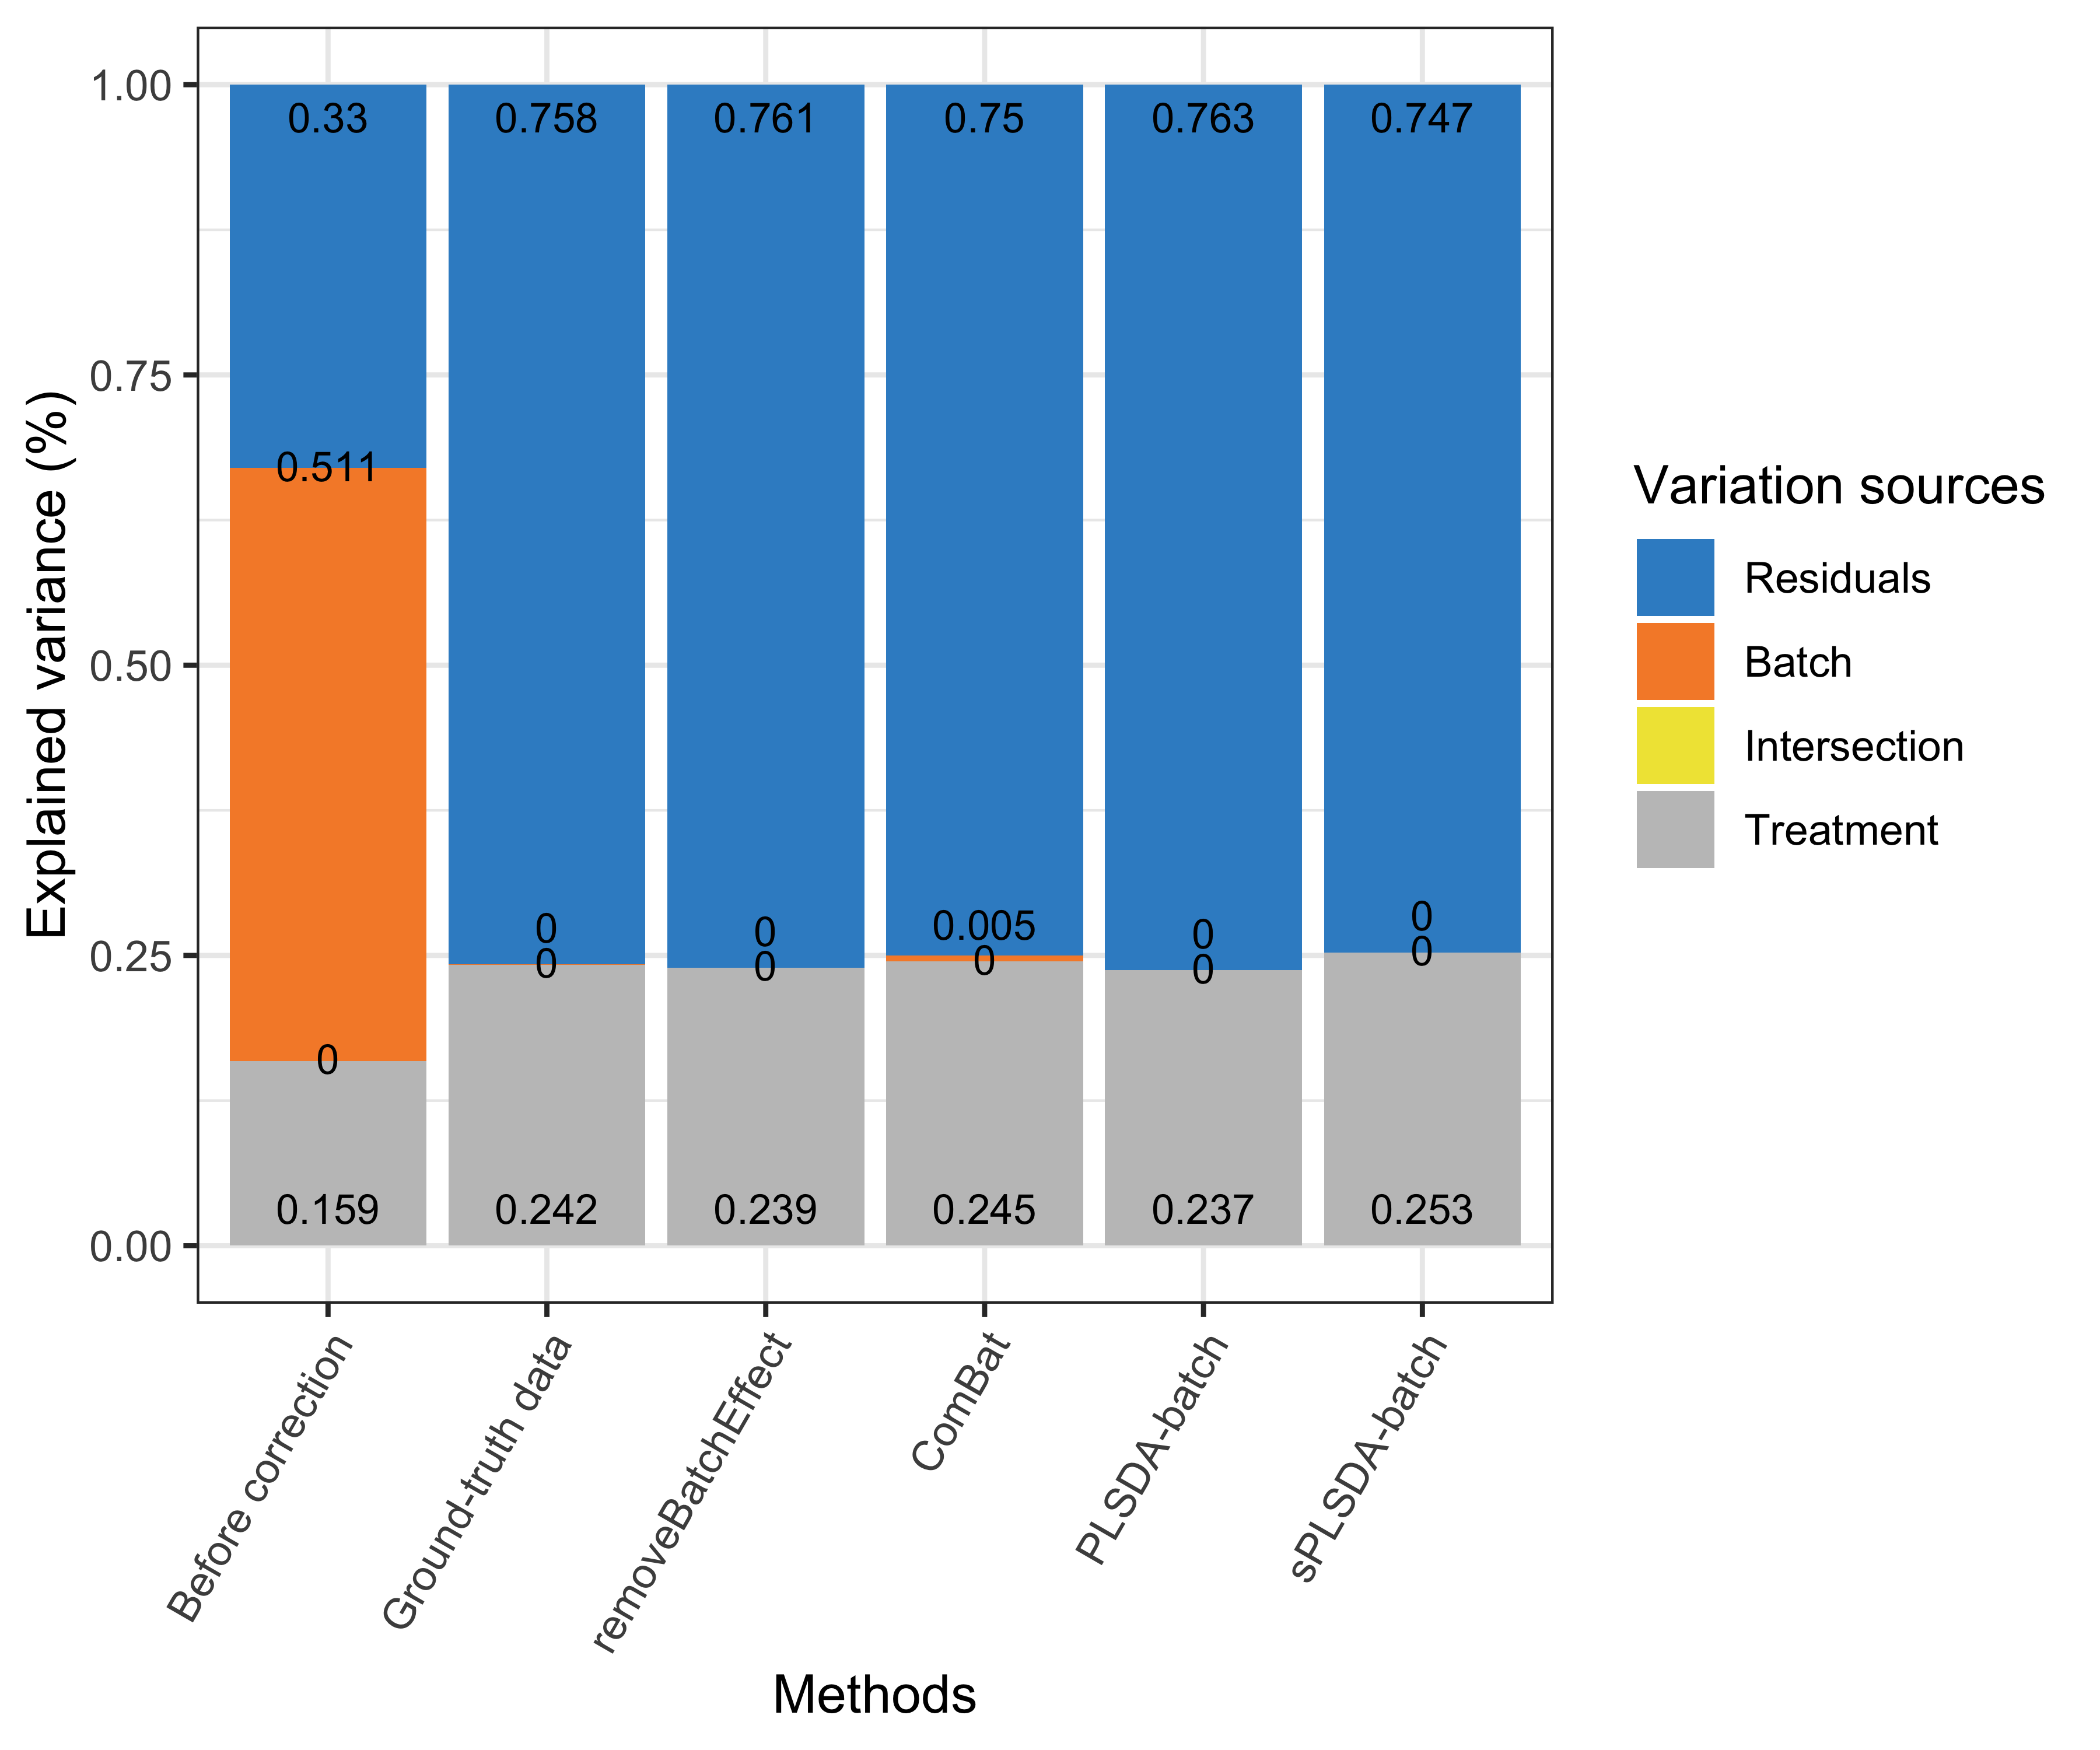
\includegraphics[width=0.7\linewidth]{PLSDAbatch_workflow_files/figure-latex/unnamed-chunk-111-1} 

}

\caption{Figure 1: Simulation studies (two batch groups): comparison of explained variance before and after batch effect correction for the balanced batch × treatment design.}\label{fig:unnamed-chunk-111}
\end{figure}

Efficient batch effect correction methods should generate data with a null proportion of variance explained by batch effects, and a proportion of variance explained by treatment that is larger compared to the original data, as shown in the figure above original data and ground-truth data.

For a balanced batch \(\times\) treatment design, we observed no intersection shared between treatment and batch variance, as expected. All methods successfully removed batch variance and preserved (or slightly increased) treatment variance (sPLSDA-batch), with the exception of ComBat where a very small amount of batch variance remained.

\begin{Shaded}
\begin{Highlighting}[]
\DocumentationTok{\#\#\#\#\#\#\#\#\#\#\#\#\#\#\#\#\#\#\#\#\#\#\#\#\#\#\#\#\#\#\#\#\#\#\#\#\#\#\#\#\#\#\#\#\#\#\#\#\#\#\#\#\#\#\#\#\#\#\#\#\#\#\#\#\#\#\#\#\#\#\#\#\#\#\#\#\#\#\#\#}
\CommentTok{\# individual variance (R2)}
\DocumentationTok{\#\# boxplot}
\CommentTok{\# class}
\NormalTok{gclass }\OtherTok{\textless{}{-}} \FunctionTok{c}\NormalTok{(}\FunctionTok{rep}\NormalTok{(}\StringTok{\textquotesingle{}Treatment only\textquotesingle{}}\NormalTok{, p\_trt\_relevant), }
            \FunctionTok{rep}\NormalTok{(}\StringTok{\textquotesingle{}Batch only\textquotesingle{}}\NormalTok{, (p\_total }\SpecialCharTok{{-}}\NormalTok{ p\_trt\_relevant)))}
\NormalTok{gclass[}\FunctionTok{intersect}\NormalTok{(true.trt, true.batch)] }\OtherTok{=} \StringTok{\textquotesingle{}Treatment \& batch\textquotesingle{}}
\NormalTok{gclass[}\FunctionTok{setdiff}\NormalTok{(}\DecValTok{1}\SpecialCharTok{:}\NormalTok{p\_total, }\FunctionTok{union}\NormalTok{(true.trt, true.batch))] }\OtherTok{=} \StringTok{\textquotesingle{}No effect\textquotesingle{}}

\NormalTok{gclass }\OtherTok{\textless{}{-}} \FunctionTok{factor}\NormalTok{(gclass, }\AttributeTok{levels =} \FunctionTok{c}\NormalTok{(}\StringTok{\textquotesingle{}Treatment \& batch\textquotesingle{}}\NormalTok{, }
                                    \StringTok{\textquotesingle{}Treatment only\textquotesingle{}}\NormalTok{, }
                                    \StringTok{\textquotesingle{}Batch only\textquotesingle{}}\NormalTok{, }
                                    \StringTok{\textquotesingle{}No effect\textquotesingle{}}\NormalTok{))}

\NormalTok{before.r2.df.ggp }\OtherTok{\textless{}{-}} \FunctionTok{data.frame}\NormalTok{(}\AttributeTok{r2 =} \FunctionTok{c}\NormalTok{(}\FunctionTok{rowMeans}\NormalTok{(r2.trt.before), }
                                      \FunctionTok{rowMeans}\NormalTok{(r2.batch.before)), }
                               \AttributeTok{type =} \FunctionTok{as.factor}\NormalTok{(}\FunctionTok{rep}\NormalTok{(}\FunctionTok{c}\NormalTok{(}\StringTok{\textquotesingle{}Treatment\textquotesingle{}}\NormalTok{,}\StringTok{\textquotesingle{}Batch\textquotesingle{}}\NormalTok{), }
                                                    \AttributeTok{each =} \DecValTok{300}\NormalTok{)),}
                               \AttributeTok{class =} \FunctionTok{rep}\NormalTok{(gclass,}\DecValTok{2}\NormalTok{))}
\NormalTok{clean.r2.df.ggp }\OtherTok{\textless{}{-}} \FunctionTok{data.frame}\NormalTok{(}\AttributeTok{r2 =} \FunctionTok{c}\NormalTok{(}\FunctionTok{rowMeans}\NormalTok{(r2.trt.clean), }
                                     \FunctionTok{rowMeans}\NormalTok{(r2.batch.clean)), }
                              \AttributeTok{type =} \FunctionTok{as.factor}\NormalTok{(}\FunctionTok{rep}\NormalTok{(}\FunctionTok{c}\NormalTok{(}\StringTok{\textquotesingle{}Treatment\textquotesingle{}}\NormalTok{,}\StringTok{\textquotesingle{}Batch\textquotesingle{}}\NormalTok{), }
                                                   \AttributeTok{each =} \DecValTok{300}\NormalTok{)),}
                              \AttributeTok{class =} \FunctionTok{rep}\NormalTok{(gclass,}\DecValTok{2}\NormalTok{))}
\NormalTok{rbe.r2.df.ggp }\OtherTok{\textless{}{-}} \FunctionTok{data.frame}\NormalTok{(}\AttributeTok{r2 =} \FunctionTok{c}\NormalTok{(}\FunctionTok{rowMeans}\NormalTok{(r2.trt.rbe), }
                                   \FunctionTok{rowMeans}\NormalTok{(r2.batch.rbe)), }
                            \AttributeTok{type =} \FunctionTok{as.factor}\NormalTok{(}\FunctionTok{rep}\NormalTok{(}\FunctionTok{c}\NormalTok{(}\StringTok{\textquotesingle{}Treatment\textquotesingle{}}\NormalTok{,}\StringTok{\textquotesingle{}Batch\textquotesingle{}}\NormalTok{), }
                                                 \AttributeTok{each =} \DecValTok{300}\NormalTok{)),}
                            \AttributeTok{class =} \FunctionTok{rep}\NormalTok{(gclass,}\DecValTok{2}\NormalTok{))}
\NormalTok{combat.r2.df.ggp }\OtherTok{\textless{}{-}} \FunctionTok{data.frame}\NormalTok{(}\AttributeTok{r2 =} \FunctionTok{c}\NormalTok{(}\FunctionTok{rowMeans}\NormalTok{(r2.trt.combat), }
                                      \FunctionTok{rowMeans}\NormalTok{(r2.batch.combat)), }
                               \AttributeTok{type =} \FunctionTok{as.factor}\NormalTok{(}\FunctionTok{rep}\NormalTok{(}\FunctionTok{c}\NormalTok{(}\StringTok{\textquotesingle{}Treatment\textquotesingle{}}\NormalTok{,}\StringTok{\textquotesingle{}Batch\textquotesingle{}}\NormalTok{), }
                                                    \AttributeTok{each =} \DecValTok{300}\NormalTok{)),}
                               \AttributeTok{class =} \FunctionTok{rep}\NormalTok{(gclass,}\DecValTok{2}\NormalTok{))}
\NormalTok{plsda\_batch.r2.df.ggp }\OtherTok{\textless{}{-}} \FunctionTok{data.frame}\NormalTok{(}\AttributeTok{r2 =} \FunctionTok{c}\NormalTok{(}\FunctionTok{rowMeans}\NormalTok{(r2.trt.plsdab), }
                                           \FunctionTok{rowMeans}\NormalTok{(r2.batch.plsdab)), }
                                    \AttributeTok{type =} \FunctionTok{as.factor}\NormalTok{(}\FunctionTok{rep}\NormalTok{(}\FunctionTok{c}\NormalTok{(}\StringTok{\textquotesingle{}Treatment\textquotesingle{}}\NormalTok{,}\StringTok{\textquotesingle{}Batch\textquotesingle{}}\NormalTok{), }
                                                         \AttributeTok{each =} \DecValTok{300}\NormalTok{)),}
                                    \AttributeTok{class =} \FunctionTok{rep}\NormalTok{(gclass,}\DecValTok{2}\NormalTok{))}
\NormalTok{splsda\_batch.r2.df.ggp }\OtherTok{\textless{}{-}} 
  \FunctionTok{data.frame}\NormalTok{(}\AttributeTok{r2 =} \FunctionTok{c}\NormalTok{(}\FunctionTok{rowMeans}\NormalTok{(r2.trt.splsdab), }
                    \FunctionTok{rowMeans}\NormalTok{(r2.batch.splsdab)), }
             \AttributeTok{type =} \FunctionTok{as.factor}\NormalTok{(}\FunctionTok{rep}\NormalTok{(}\FunctionTok{c}\NormalTok{(}\StringTok{\textquotesingle{}Treatment\textquotesingle{}}\NormalTok{,}\StringTok{\textquotesingle{}Batch\textquotesingle{}}\NormalTok{), }
                                  \AttributeTok{each =} \DecValTok{300}\NormalTok{)),}
             \AttributeTok{class =} \FunctionTok{rep}\NormalTok{(gclass,}\DecValTok{2}\NormalTok{))}

\NormalTok{all.r2.df.ggp }\OtherTok{\textless{}{-}} \FunctionTok{rbind}\NormalTok{(before.r2.df.ggp, clean.r2.df.ggp,}
\NormalTok{                       rbe.r2.df.ggp, combat.r2.df.ggp,}
\NormalTok{                       plsda\_batch.r2.df.ggp, splsda\_batch.r2.df.ggp)}

\NormalTok{all.r2.df.ggp}\SpecialCharTok{$}\NormalTok{methods }\OtherTok{\textless{}{-}} \FunctionTok{rep}\NormalTok{(}\FunctionTok{c}\NormalTok{(}\StringTok{\textquotesingle{}Before correction\textquotesingle{}}\NormalTok{, }
                               \StringTok{\textquotesingle{}Ground{-}truth data\textquotesingle{}}\NormalTok{, }
                               \StringTok{\textquotesingle{}removeBatchEffect\textquotesingle{}}\NormalTok{, }
                               \StringTok{\textquotesingle{}ComBat\textquotesingle{}}\NormalTok{,}
                               \StringTok{\textquotesingle{}PLSDA{-}batch\textquotesingle{}}\NormalTok{, }
                               \StringTok{\textquotesingle{}sPLSDA{-}batch\textquotesingle{}}\NormalTok{), }\AttributeTok{each =} \DecValTok{600}\NormalTok{)}

\NormalTok{all.r2.df.ggp}\SpecialCharTok{$}\NormalTok{methods }\OtherTok{\textless{}{-}} \FunctionTok{factor}\NormalTok{(all.r2.df.ggp}\SpecialCharTok{$}\NormalTok{methods, }
                                \AttributeTok{levels =} \FunctionTok{unique}\NormalTok{(all.r2.df.ggp}\SpecialCharTok{$}\NormalTok{methods))}

\FunctionTok{ggplot}\NormalTok{(all.r2.df.ggp, }\FunctionTok{aes}\NormalTok{(}\AttributeTok{x =}\NormalTok{ type, }\AttributeTok{y =}\NormalTok{ r2, }\AttributeTok{fill =}\NormalTok{ class)) }\SpecialCharTok{+}
  \FunctionTok{geom\_boxplot}\NormalTok{(}\AttributeTok{alpha =} \FloatTok{0.80}\NormalTok{) }\SpecialCharTok{+}
  \FunctionTok{theme\_bw}\NormalTok{() }\SpecialCharTok{+} 
  \FunctionTok{theme}\NormalTok{(}\AttributeTok{text =} \FunctionTok{element\_text}\NormalTok{(}\AttributeTok{size =} \DecValTok{18}\NormalTok{),}
        \AttributeTok{axis.title.x =} \FunctionTok{element\_blank}\NormalTok{(),}
        \AttributeTok{axis.title.y =} \FunctionTok{element\_blank}\NormalTok{(),}
        \AttributeTok{panel.grid.minor.x =} \FunctionTok{element\_blank}\NormalTok{(),}
        \AttributeTok{panel.grid.major.x =} \FunctionTok{element\_blank}\NormalTok{(),}
        \AttributeTok{legend.position =} \StringTok{"right"}\NormalTok{) }\SpecialCharTok{+} \FunctionTok{facet\_grid}\NormalTok{(class }\SpecialCharTok{\textasciitilde{}}\NormalTok{ methods) }\SpecialCharTok{+} 
  \FunctionTok{scale\_fill\_manual}\NormalTok{(}\AttributeTok{values=}\FunctionTok{c}\NormalTok{(}\StringTok{\textquotesingle{}dark gray\textquotesingle{}}\NormalTok{, }\FunctionTok{color.mixo}\NormalTok{(}\DecValTok{4}\NormalTok{), }
                             \FunctionTok{color.mixo}\NormalTok{(}\DecValTok{5}\NormalTok{), }\FunctionTok{color.mixo}\NormalTok{(}\DecValTok{9}\NormalTok{)))}
\end{Highlighting}
\end{Shaded}

\begin{figure}

{\centering \includegraphics[width=1\linewidth]{PLSDAbatch_workflow_files/figure-latex/unnamed-chunk-112-1} 

}

\caption{Figure 2: Simulation studies (two batch groups): R2 values for each microbial variable before and after batch effect correction for the balanced batch × treatment design.}\label{fig:unnamed-chunk-112}
\end{figure}

\begin{Shaded}
\begin{Highlighting}[]
\DocumentationTok{\#\#\#\#\#\#\#\#\#\#\#\#\#\#\#\#\#\#\#\#\#\#\#\#\#\#\#\#\#\#\#\#\#\#\#\#\#\#\#\#\#\#\#\#\#\#\#\#\#\#\#\#\#\#\#\#\#\#\#\#\#\#\#\#\#\#\#\#\#\#\#\#\#\#\#\#\#\#\#\#}
\DocumentationTok{\#\# barplot}
\CommentTok{\# class}
\NormalTok{before.r2.df.bp }\OtherTok{\textless{}{-}} 
  \FunctionTok{data.frame}\NormalTok{(}\AttributeTok{r2 =} \FunctionTok{c}\NormalTok{(}\FunctionTok{tapply}\NormalTok{(}\FunctionTok{rowMeans}\NormalTok{(r2.trt.before), gclass, sum), }
                    \FunctionTok{tapply}\NormalTok{(}\FunctionTok{rowMeans}\NormalTok{(r2.batch.before), gclass, sum)), }
             \AttributeTok{type =} \FunctionTok{as.factor}\NormalTok{(}\FunctionTok{rep}\NormalTok{(}\FunctionTok{c}\NormalTok{(}\StringTok{\textquotesingle{}Treatment\textquotesingle{}}\NormalTok{,}\StringTok{\textquotesingle{}Batch\textquotesingle{}}\NormalTok{), }\AttributeTok{each =} \DecValTok{4}\NormalTok{)),}
             \AttributeTok{class =} \FunctionTok{factor}\NormalTok{(}\FunctionTok{rep}\NormalTok{(}\FunctionTok{levels}\NormalTok{(gclass),}\DecValTok{2}\NormalTok{), }\AttributeTok{levels =} \FunctionTok{levels}\NormalTok{(gclass)))}

\NormalTok{clean.r2.df.bp }\OtherTok{\textless{}{-}} 
  \FunctionTok{data.frame}\NormalTok{(}\AttributeTok{r2 =} \FunctionTok{c}\NormalTok{(}\FunctionTok{tapply}\NormalTok{(}\FunctionTok{rowMeans}\NormalTok{(r2.trt.clean), gclass, sum), }
                    \FunctionTok{tapply}\NormalTok{(}\FunctionTok{rowMeans}\NormalTok{(r2.batch.clean), gclass, sum)), }
             \AttributeTok{type =} \FunctionTok{as.factor}\NormalTok{(}\FunctionTok{rep}\NormalTok{(}\FunctionTok{c}\NormalTok{(}\StringTok{\textquotesingle{}Treatment\textquotesingle{}}\NormalTok{,}\StringTok{\textquotesingle{}Batch\textquotesingle{}}\NormalTok{), }\AttributeTok{each =} \DecValTok{4}\NormalTok{)),}
             \AttributeTok{class =} \FunctionTok{factor}\NormalTok{(}\FunctionTok{rep}\NormalTok{(}\FunctionTok{levels}\NormalTok{(gclass),}\DecValTok{2}\NormalTok{), }\AttributeTok{levels =} \FunctionTok{levels}\NormalTok{(gclass)))}

\NormalTok{rbe.r2.df.bp }\OtherTok{\textless{}{-}} 
  \FunctionTok{data.frame}\NormalTok{(}\AttributeTok{r2 =} \FunctionTok{c}\NormalTok{(}\FunctionTok{tapply}\NormalTok{(}\FunctionTok{rowMeans}\NormalTok{(r2.trt.rbe), gclass, sum), }
                    \FunctionTok{tapply}\NormalTok{(}\FunctionTok{rowMeans}\NormalTok{(r2.batch.rbe), gclass, sum)), }
             \AttributeTok{type =} \FunctionTok{as.factor}\NormalTok{(}\FunctionTok{rep}\NormalTok{(}\FunctionTok{c}\NormalTok{(}\StringTok{\textquotesingle{}Treatment\textquotesingle{}}\NormalTok{,}\StringTok{\textquotesingle{}Batch\textquotesingle{}}\NormalTok{), }\AttributeTok{each =} \DecValTok{4}\NormalTok{)),}
             \AttributeTok{class =} \FunctionTok{factor}\NormalTok{(}\FunctionTok{rep}\NormalTok{(}\FunctionTok{levels}\NormalTok{(gclass),}\DecValTok{2}\NormalTok{), }\AttributeTok{levels =} \FunctionTok{levels}\NormalTok{(gclass)))}

\NormalTok{combat.r2.df.bp }\OtherTok{\textless{}{-}} 
  \FunctionTok{data.frame}\NormalTok{(}\AttributeTok{r2 =} \FunctionTok{c}\NormalTok{(}\FunctionTok{tapply}\NormalTok{(}\FunctionTok{rowMeans}\NormalTok{(r2.trt.combat), gclass, sum), }
                    \FunctionTok{tapply}\NormalTok{(}\FunctionTok{rowMeans}\NormalTok{(r2.batch.combat), gclass, sum)), }
             \AttributeTok{type =} \FunctionTok{as.factor}\NormalTok{(}\FunctionTok{rep}\NormalTok{(}\FunctionTok{c}\NormalTok{(}\StringTok{\textquotesingle{}Treatment\textquotesingle{}}\NormalTok{,}\StringTok{\textquotesingle{}Batch\textquotesingle{}}\NormalTok{), }\AttributeTok{each =} \DecValTok{4}\NormalTok{)),}
             \AttributeTok{class =} \FunctionTok{factor}\NormalTok{(}\FunctionTok{rep}\NormalTok{(}\FunctionTok{levels}\NormalTok{(gclass),}\DecValTok{2}\NormalTok{), }\AttributeTok{levels =} \FunctionTok{levels}\NormalTok{(gclass)))}

\NormalTok{plsda\_batch.r2.df.bp }\OtherTok{\textless{}{-}} 
  \FunctionTok{data.frame}\NormalTok{(}\AttributeTok{r2 =} \FunctionTok{c}\NormalTok{(}\FunctionTok{tapply}\NormalTok{(}\FunctionTok{rowMeans}\NormalTok{(r2.trt.plsdab), gclass, sum), }
                    \FunctionTok{tapply}\NormalTok{(}\FunctionTok{rowMeans}\NormalTok{(r2.batch.plsdab), gclass, sum)), }
             \AttributeTok{type =} \FunctionTok{as.factor}\NormalTok{(}\FunctionTok{rep}\NormalTok{(}\FunctionTok{c}\NormalTok{(}\StringTok{\textquotesingle{}Treatment\textquotesingle{}}\NormalTok{,}\StringTok{\textquotesingle{}Batch\textquotesingle{}}\NormalTok{), }\AttributeTok{each =} \DecValTok{4}\NormalTok{)),}
             \AttributeTok{class =} \FunctionTok{factor}\NormalTok{(}\FunctionTok{rep}\NormalTok{(}\FunctionTok{levels}\NormalTok{(gclass),}\DecValTok{2}\NormalTok{), }\AttributeTok{levels =} \FunctionTok{levels}\NormalTok{(gclass)))}

\NormalTok{splsda\_batch.r2.df.bp }\OtherTok{\textless{}{-}} 
  \FunctionTok{data.frame}\NormalTok{(}\AttributeTok{r2 =} \FunctionTok{c}\NormalTok{(}\FunctionTok{tapply}\NormalTok{(}\FunctionTok{rowMeans}\NormalTok{(r2.trt.splsdab), gclass, sum), }
                    \FunctionTok{tapply}\NormalTok{(}\FunctionTok{rowMeans}\NormalTok{(r2.batch.splsdab), gclass, sum)), }
             \AttributeTok{type =} \FunctionTok{as.factor}\NormalTok{(}\FunctionTok{rep}\NormalTok{(}\FunctionTok{c}\NormalTok{(}\StringTok{\textquotesingle{}Treatment\textquotesingle{}}\NormalTok{,}\StringTok{\textquotesingle{}Batch\textquotesingle{}}\NormalTok{), }\AttributeTok{each =} \DecValTok{4}\NormalTok{)),}
             \AttributeTok{class =} \FunctionTok{factor}\NormalTok{(}\FunctionTok{rep}\NormalTok{(}\FunctionTok{levels}\NormalTok{(gclass),}\DecValTok{2}\NormalTok{), }\AttributeTok{levels =} \FunctionTok{levels}\NormalTok{(gclass)))}


\NormalTok{all.r2.df.bp }\OtherTok{\textless{}{-}} \FunctionTok{rbind}\NormalTok{(before.r2.df.bp, clean.r2.df.bp,}
\NormalTok{                      rbe.r2.df.bp, combat.r2.df.bp,}
\NormalTok{                      plsda\_batch.r2.df.bp, splsda\_batch.r2.df.bp)}


\NormalTok{all.r2.df.bp}\SpecialCharTok{$}\NormalTok{methods }\OtherTok{\textless{}{-}} \FunctionTok{rep}\NormalTok{(}\FunctionTok{c}\NormalTok{(}\StringTok{\textquotesingle{}Before correction\textquotesingle{}}\NormalTok{, }
                              \StringTok{\textquotesingle{}Ground{-}truth data\textquotesingle{}}\NormalTok{, }
                              \StringTok{\textquotesingle{}removeBatchEffect\textquotesingle{}}\NormalTok{, }\StringTok{\textquotesingle{}ComBat\textquotesingle{}}\NormalTok{,}
                              \StringTok{\textquotesingle{}PLSDA{-}batch\textquotesingle{}}\NormalTok{, }\StringTok{\textquotesingle{}sPLSDA{-}batch\textquotesingle{}}\NormalTok{), }\AttributeTok{each =} \DecValTok{8}\NormalTok{)}

\NormalTok{all.r2.df.bp}\SpecialCharTok{$}\NormalTok{methods }\OtherTok{\textless{}{-}} \FunctionTok{factor}\NormalTok{(all.r2.df.bp}\SpecialCharTok{$}\NormalTok{methods, }
                               \AttributeTok{levels =} \FunctionTok{unique}\NormalTok{(all.r2.df.bp}\SpecialCharTok{$}\NormalTok{methods))}

\FunctionTok{ggplot}\NormalTok{(all.r2.df.bp, }\FunctionTok{aes}\NormalTok{(}\AttributeTok{x =}\NormalTok{ type, }\AttributeTok{y =}\NormalTok{ r2, }\AttributeTok{fill =}\NormalTok{ class)) }\SpecialCharTok{+}
  \FunctionTok{geom\_bar}\NormalTok{(}\AttributeTok{stat=}\StringTok{"identity"}\NormalTok{) }\SpecialCharTok{+} 
  \FunctionTok{theme\_bw}\NormalTok{() }\SpecialCharTok{+} 
  \FunctionTok{theme}\NormalTok{(}\AttributeTok{text =} \FunctionTok{element\_text}\NormalTok{(}\AttributeTok{size =} \DecValTok{18}\NormalTok{),}
        \AttributeTok{axis.title.x =} \FunctionTok{element\_blank}\NormalTok{(),}
        \AttributeTok{axis.title.y =} \FunctionTok{element\_blank}\NormalTok{(),}
        \AttributeTok{panel.grid.minor.x =} \FunctionTok{element\_blank}\NormalTok{(),}
        \AttributeTok{panel.grid.major.x =} \FunctionTok{element\_blank}\NormalTok{(),}
        \AttributeTok{legend.position =} \StringTok{"right"}\NormalTok{) }\SpecialCharTok{+} \FunctionTok{facet\_grid}\NormalTok{(class }\SpecialCharTok{\textasciitilde{}}\NormalTok{ methods) }\SpecialCharTok{+} 
  \FunctionTok{scale\_fill\_manual}\NormalTok{(}\AttributeTok{values=}\FunctionTok{c}\NormalTok{(}\StringTok{\textquotesingle{}dark gray\textquotesingle{}}\NormalTok{, }\FunctionTok{color.mixo}\NormalTok{(}\DecValTok{4}\NormalTok{), }
                             \FunctionTok{color.mixo}\NormalTok{(}\DecValTok{5}\NormalTok{), }\FunctionTok{color.mixo}\NormalTok{(}\DecValTok{9}\NormalTok{)))}
\end{Highlighting}
\end{Shaded}

\begin{figure}

{\centering 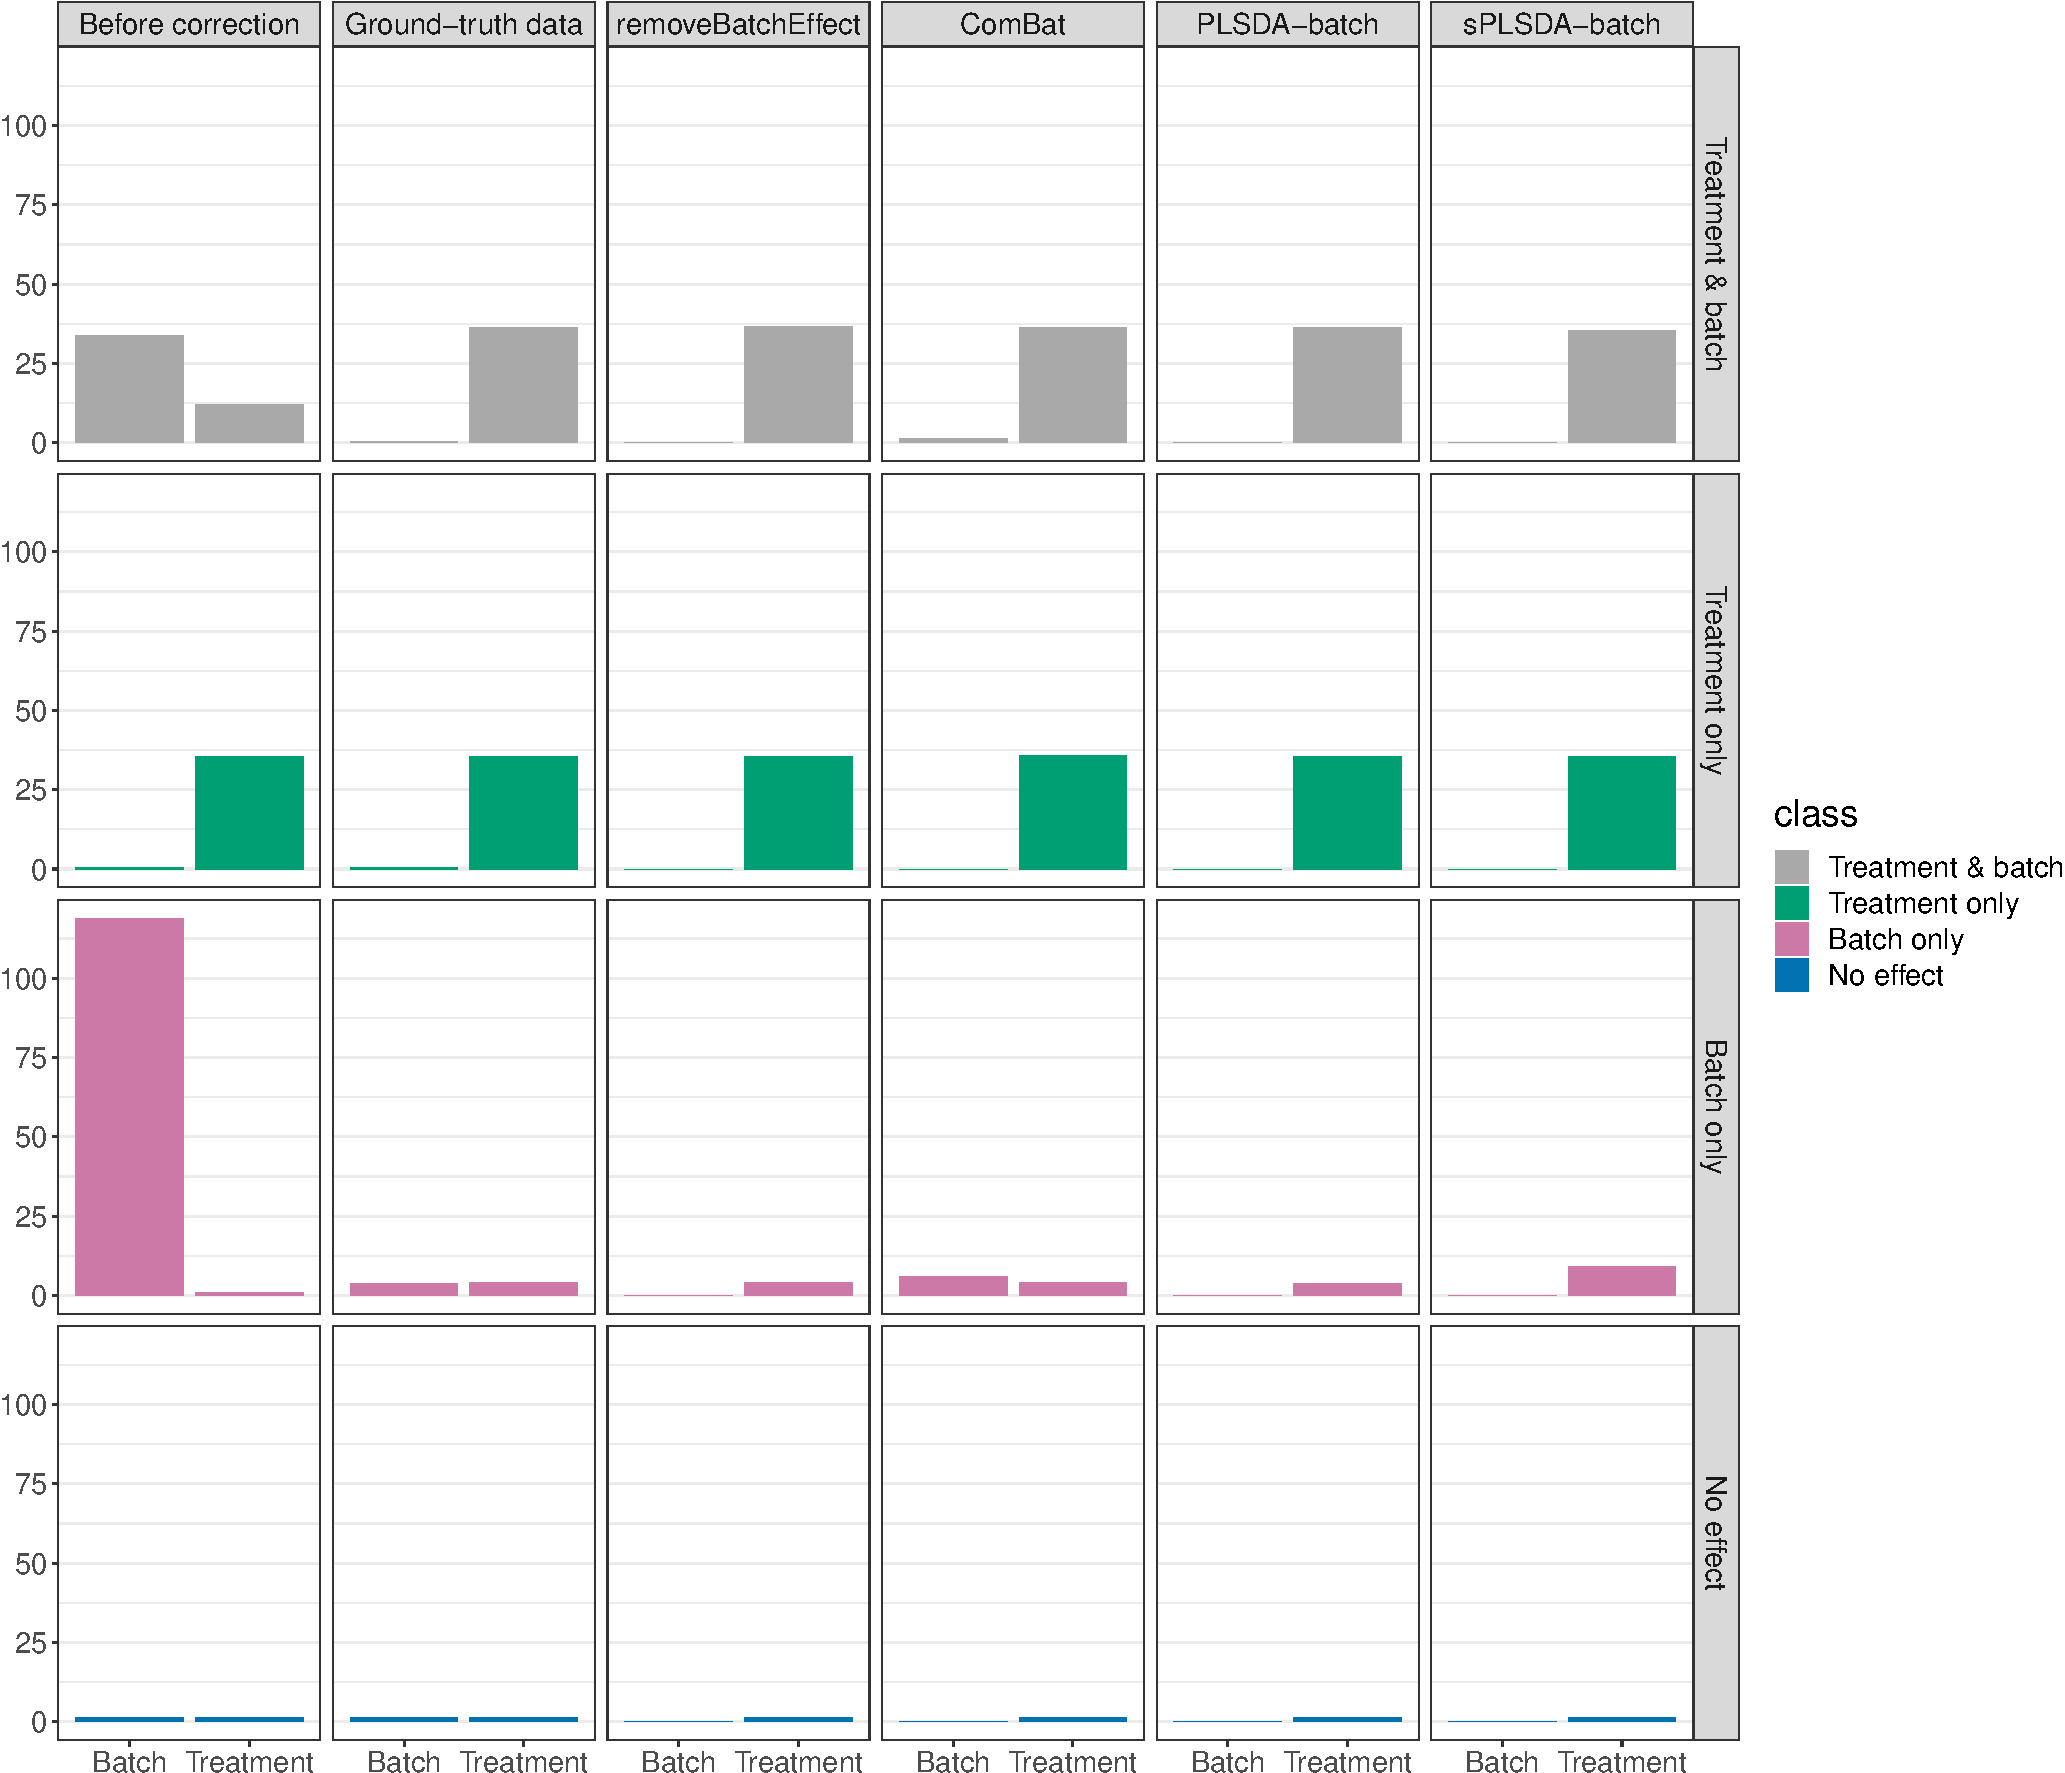
\includegraphics[width=1\linewidth]{PLSDAbatch_workflow_files/figure-latex/unnamed-chunk-113-1} 

}

\caption{Figure 3: Simulation studies (two batch groups): the sum of R2 values for each microbial variable before and after batch effect correction for the balanced batch × treatment design.}\label{fig:unnamed-chunk-113}
\end{figure}

We estimated the proportion of variance explained by treatment and batch effects for each variable using the \(R^2\) value. removeBatchEffect and PLSDA-batch had the best performance, with results very similar to the ground-truth data. ComBat retained more batch variance of variables with batch effects only, and with both batch and treatment effects, indicating an incomplete removal of batch effects. This result is in agreement with the overall pRDA evaluation described earlier. For sPLSDA-batch, variables with no treatment effect (batch effects only) included a slight amount of (spurious) treatment variance. This was also observed in pRDA evaluation. However, sPLSDA-batch performed as well as PLSDA-batch when the simulated data did not include variables with both batch and treatment effects.

\begin{Shaded}
\begin{Highlighting}[]
\CommentTok{\# precision \& recall \& F1 (ANOVA \& sPLSDA)}
\DocumentationTok{\#\# mean}
\NormalTok{acc\_mean }\OtherTok{\textless{}{-}} \FunctionTok{rbind}\NormalTok{(}\FunctionTok{colMeans}\NormalTok{(precision\_limma), }\FunctionTok{colMeans}\NormalTok{(recall\_limma), }
                  \FunctionTok{colMeans}\NormalTok{(F1\_limma), }\FunctionTok{c}\NormalTok{(}\FunctionTok{colMeans}\NormalTok{(auc\_splsda), }\AttributeTok{sva =} \ConstantTok{NA}\NormalTok{))}
\FunctionTok{rownames}\NormalTok{(acc\_mean) }\OtherTok{\textless{}{-}} \FunctionTok{c}\NormalTok{(}\StringTok{\textquotesingle{}Precision\textquotesingle{}}\NormalTok{, }\StringTok{\textquotesingle{}Recall\textquotesingle{}}\NormalTok{, }\StringTok{\textquotesingle{}F1\textquotesingle{}}\NormalTok{, }\StringTok{\textquotesingle{}AUC\textquotesingle{}}\NormalTok{)}
\FunctionTok{colnames}\NormalTok{(acc\_mean) }\OtherTok{\textless{}{-}} \FunctionTok{c}\NormalTok{(}\StringTok{\textquotesingle{}Before correction\textquotesingle{}}\NormalTok{, }\StringTok{\textquotesingle{}Ground{-}truth data\textquotesingle{}}\NormalTok{, }
                        \StringTok{\textquotesingle{}removeBatchEffect\textquotesingle{}}\NormalTok{, }\StringTok{\textquotesingle{}ComBat\textquotesingle{}}\NormalTok{, }
                        \StringTok{\textquotesingle{}PLSDA{-}batch\textquotesingle{}}\NormalTok{, }\StringTok{\textquotesingle{}sPLSDA{-}batch\textquotesingle{}}\NormalTok{, }\StringTok{\textquotesingle{}SVA\textquotesingle{}}\NormalTok{)}
\NormalTok{acc\_mean }\OtherTok{\textless{}{-}} \FunctionTok{format}\NormalTok{(acc\_mean, }\AttributeTok{digits =} \DecValTok{3}\NormalTok{)}
\NormalTok{knitr}\SpecialCharTok{::}\FunctionTok{kable}\NormalTok{(acc\_mean, }\AttributeTok{caption =} \StringTok{\textquotesingle{}Table 3: Simulation studies (two batch groups): summary of accuracy measurements before and after batch effect correction for the balanced batch × treatment design (mean).\textquotesingle{}}\NormalTok{)}
\end{Highlighting}
\end{Shaded}

\begin{table}

\caption{\label{tab:unnamed-chunk-114}Table 3: Simulation studies (two batch groups): summary of accuracy measurements before and after batch effect correction for the balanced batch × treatment design (mean).}
\centering
\begin{tabular}[t]{l|l|l|l|l|l|l|l}
\hline
  & Before correction & Ground-truth data & removeBatchEffect & ComBat & PLSDA-batch & sPLSDA-batch & SVA\\
\hline
Precision & 0.984 & 0.952 & 0.950 & 0.952 & 0.952 & 0.807 & 0.957\\
\hline
Recall & 0.674 & 0.900 & 0.910 & 0.911 & 0.910 & 0.910 & 0.934\\
\hline
F1 & 0.799 & 0.923 & 0.927 & 0.929 & 0.929 & 0.851 & 0.944\\
\hline
AUC & 0.944 & 0.964 & 0.968 & 0.968 & 0.969 & 0.954 & NA\\
\hline
\end{tabular}
\end{table}

The results from the accuracy measures combined with variable selection highlight the importance of removing batch effects as both F1 score and AUC largely improved compared to the original data.

Starting from the original data compared to the ground-truth data, selected variables had a higher precision, lower recall and lower AUC, indicating a smaller number of variables selected with an actual treatment effect. Combined with univariate one-way ANOVA, SVA performed best with the highest, and sometimes greater, accuracy measurements than the ground-truth data. The other methods led to similar performance with the exception of sPLSDA-batch, which selected more false positives than the other methods. PLSDA-batch led to a slightly better AUC than the other methods.

\begin{Shaded}
\begin{Highlighting}[]
\DocumentationTok{\#\# sd}
\NormalTok{acc\_sd }\OtherTok{\textless{}{-}} \FunctionTok{rbind}\NormalTok{(}\FunctionTok{apply}\NormalTok{(precision\_limma, }\DecValTok{2}\NormalTok{, sd), }\FunctionTok{apply}\NormalTok{(recall\_limma, }\DecValTok{2}\NormalTok{, sd), }
                \FunctionTok{apply}\NormalTok{(F1\_limma, }\DecValTok{2}\NormalTok{, sd), }\FunctionTok{c}\NormalTok{(}\FunctionTok{apply}\NormalTok{(auc\_splsda, }\DecValTok{2}\NormalTok{, sd), }\ConstantTok{NA}\NormalTok{))}
\FunctionTok{rownames}\NormalTok{(acc\_sd) }\OtherTok{\textless{}{-}} \FunctionTok{c}\NormalTok{(}\StringTok{\textquotesingle{}Precision\textquotesingle{}}\NormalTok{, }\StringTok{\textquotesingle{}Recall\textquotesingle{}}\NormalTok{, }\StringTok{\textquotesingle{}F1\textquotesingle{}}\NormalTok{, }\StringTok{\textquotesingle{}AUC\textquotesingle{}}\NormalTok{)}
\FunctionTok{colnames}\NormalTok{(acc\_sd) }\OtherTok{\textless{}{-}} \FunctionTok{c}\NormalTok{(}\StringTok{\textquotesingle{}Before correction\textquotesingle{}}\NormalTok{, }\StringTok{\textquotesingle{}Ground{-}truth data\textquotesingle{}}\NormalTok{, }
                      \StringTok{\textquotesingle{}removeBatchEffect\textquotesingle{}}\NormalTok{, }\StringTok{\textquotesingle{}ComBat\textquotesingle{}}\NormalTok{, }
                      \StringTok{\textquotesingle{}PLSDA{-}batch\textquotesingle{}}\NormalTok{, }\StringTok{\textquotesingle{}sPLSDA{-}batch\textquotesingle{}}\NormalTok{, }\StringTok{\textquotesingle{}SVA\textquotesingle{}}\NormalTok{)}
\NormalTok{acc\_sd }\OtherTok{\textless{}{-}} \FunctionTok{format}\NormalTok{(acc\_sd, }\AttributeTok{digits =} \DecValTok{1}\NormalTok{)}
\NormalTok{knitr}\SpecialCharTok{::}\FunctionTok{kable}\NormalTok{(acc\_sd, }\AttributeTok{caption =} \StringTok{\textquotesingle{}Table 4: Simulation studies (two batch groups): summary of accuracy measurements before and after batch effect correction for the balanced batch × treatment design (standard deviation).\textquotesingle{}}\NormalTok{)}
\end{Highlighting}
\end{Shaded}

\begin{table}

\caption{\label{tab:unnamed-chunk-115}Table 4: Simulation studies (two batch groups): summary of accuracy measurements before and after batch effect correction for the balanced batch × treatment design (standard deviation).}
\centering
\begin{tabular}[t]{l|l|l|l|l|l|l|l}
\hline
  & Before correction & Ground-truth data & removeBatchEffect & ComBat & PLSDA-batch & sPLSDA-batch & SVA\\
\hline
Precision & 0.04 & 0.08 & 0.09 & 0.08 & 0.08 & 0.11 & 0.06\\
\hline
Recall & 0.03 & 0.03 & 0.03 & 0.03 & 0.03 & 0.03 & 0.03\\
\hline
F1 & 0.02 & 0.05 & 0.05 & 0.05 & 0.05 & 0.06 & 0.04\\
\hline
AUC & 0.02 & 0.02 & 0.02 & 0.02 & 0.01 & 0.02 & NA\\
\hline
\end{tabular}
\end{table}

\hypertarget{unbalanced-batch-times-treatment-design-1}{%
\subsection{\texorpdfstring{Unbalanced batch \(\times\) treatment design}{Unbalanced batch \textbackslash times treatment design}}\label{unbalanced-batch-times-treatment-design-1}}

The unbalanced design included 4 and 16 samples from batch1 and batch2 respectively in trt1, 16 and 4 samples from batch1 and batch2 in trt2.

\textbf{Table 5: Unbalanced batch} \(\times\) treatment design in the simulation study

\begin{longtable}[]{@{}ccc@{}}
\toprule()
& Trt1 & Trt2 \\
\midrule()
\endhead
Batch1 & 4 & 16 \\
Batch2 & 16 & 4 \\
\bottomrule()
\end{longtable}

\begin{Shaded}
\begin{Highlighting}[]
\NormalTok{nitr }\OtherTok{\textless{}{-}} \DecValTok{50}
\NormalTok{N }\OtherTok{=} \DecValTok{40}
\NormalTok{p\_total }\OtherTok{=} \DecValTok{300}
\NormalTok{p\_trt\_relevant }\OtherTok{=} \DecValTok{100} 
\NormalTok{p\_bat\_relevant }\OtherTok{=} \DecValTok{200} 

\CommentTok{\# global variance (RDA)}
\NormalTok{gvar.before }\OtherTok{\textless{}{-}}\NormalTok{ gvar.clean }\OtherTok{\textless{}{-}} 
\NormalTok{  gvar.rbe }\OtherTok{\textless{}{-}}\NormalTok{ gvar.combat }\OtherTok{\textless{}{-}} 
\NormalTok{  gvar.wplsdab }\OtherTok{\textless{}{-}}\NormalTok{ gvar.swplsdab }\OtherTok{\textless{}{-}} 
\NormalTok{  gvar.plsdab }\OtherTok{\textless{}{-}}\NormalTok{ gvar.splsdab }\OtherTok{\textless{}{-}} \FunctionTok{data.frame}\NormalTok{(}\AttributeTok{treatment =} \ConstantTok{NA}\NormalTok{, }\AttributeTok{batch =} \ConstantTok{NA}\NormalTok{,  }
                                            \AttributeTok{intersection =} \ConstantTok{NA}\NormalTok{, }
                                            \AttributeTok{residual =} \ConstantTok{NA}\NormalTok{)}

\CommentTok{\# individual variance (R2)}
\NormalTok{r2.trt.before }\OtherTok{\textless{}{-}}\NormalTok{ r2.trt.clean }\OtherTok{\textless{}{-}} 
\NormalTok{  r2.trt.rbe  }\OtherTok{\textless{}{-}}\NormalTok{ r2.trt.combat }\OtherTok{\textless{}{-}} 
\NormalTok{  r2.trt.wplsdab }\OtherTok{\textless{}{-}}\NormalTok{ r2.trt.swplsdab }\OtherTok{\textless{}{-}}
\NormalTok{  r2.trt.plsdab }\OtherTok{\textless{}{-}}\NormalTok{ r2.trt.splsdab }\OtherTok{\textless{}{-}} \FunctionTok{data.frame}\NormalTok{(}\FunctionTok{matrix}\NormalTok{(}\ConstantTok{NA}\NormalTok{, }\AttributeTok{nrow =}\NormalTok{ p\_total, }
                                                       \AttributeTok{ncol =}\NormalTok{ nitr))}
\NormalTok{r2.batch.before }\OtherTok{\textless{}{-}}\NormalTok{ r2.batch.clean }\OtherTok{\textless{}{-}} 
\NormalTok{  r2.batch.rbe  }\OtherTok{\textless{}{-}}\NormalTok{ r2.batch.combat }\OtherTok{\textless{}{-}} 
\NormalTok{  r2.batch.wplsdab }\OtherTok{\textless{}{-}}\NormalTok{ r2.batch.swplsdab }\OtherTok{\textless{}{-}}
\NormalTok{  r2.batch.plsdab }\OtherTok{\textless{}{-}}\NormalTok{ r2.batch.splsdab }\OtherTok{\textless{}{-}} \FunctionTok{data.frame}\NormalTok{(}\FunctionTok{matrix}\NormalTok{(}\ConstantTok{NA}\NormalTok{, }\AttributeTok{nrow =}\NormalTok{ p\_total, }
                                                           \AttributeTok{ncol =}\NormalTok{ nitr))}

\CommentTok{\# precision \& recall \& F1 (ANOVA)}
\NormalTok{precision\_limma }\OtherTok{\textless{}{-}}\NormalTok{ recall\_limma }\OtherTok{\textless{}{-}}\NormalTok{ F1\_limma }\OtherTok{\textless{}{-}} 
  \FunctionTok{data.frame}\NormalTok{(}\AttributeTok{before =} \ConstantTok{NA}\NormalTok{, }\AttributeTok{clean =} \ConstantTok{NA}\NormalTok{, }
             \AttributeTok{rbe =} \ConstantTok{NA}\NormalTok{, }\AttributeTok{combat =} \ConstantTok{NA}\NormalTok{, }
             \AttributeTok{wplsda\_batch =} \ConstantTok{NA}\NormalTok{, }\AttributeTok{swplsda\_batch =} \ConstantTok{NA}\NormalTok{, }
             \AttributeTok{sva =} \ConstantTok{NA}\NormalTok{)}

\CommentTok{\# auc (splsda)}
\NormalTok{auc\_splsda }\OtherTok{\textless{}{-}} 
  \FunctionTok{data.frame}\NormalTok{(}\AttributeTok{before =} \ConstantTok{NA}\NormalTok{, }\AttributeTok{clean =} \ConstantTok{NA}\NormalTok{, }
             \AttributeTok{rbe =} \ConstantTok{NA}\NormalTok{, }\AttributeTok{combat =} \ConstantTok{NA}\NormalTok{, }
             \AttributeTok{wplsda\_batch =} \ConstantTok{NA}\NormalTok{, }\AttributeTok{swplsda\_batch =} \ConstantTok{NA}\NormalTok{)}


\FunctionTok{set.seed}\NormalTok{(}\DecValTok{70}\NormalTok{)}
\NormalTok{data.cor.res }\OtherTok{=} \FunctionTok{corStruct}\NormalTok{(}\AttributeTok{p =} \DecValTok{300}\NormalTok{, }\AttributeTok{zero\_prob =} \FloatTok{0.7}\NormalTok{)}

\ControlFlowTok{for}\NormalTok{(i }\ControlFlowTok{in} \DecValTok{1}\SpecialCharTok{:}\NormalTok{ nitr)\{}
  \DocumentationTok{\#\#\# initial setup }\AlertTok{\#\#\#}
\NormalTok{  simulation }\OtherTok{\textless{}{-}} \FunctionTok{simData\_mnegbinom}\NormalTok{(}\AttributeTok{batch.group =} \DecValTok{2}\NormalTok{,}
                                  \AttributeTok{mean.batch =} \DecValTok{7}\NormalTok{, }
                                  \AttributeTok{sd.batch =} \DecValTok{8}\NormalTok{, }
                                  \AttributeTok{mean.trt =} \DecValTok{3}\NormalTok{, }
                                  \AttributeTok{sd.trt =} \DecValTok{2}\NormalTok{, }
                                  \AttributeTok{mean.bg =} \DecValTok{0}\NormalTok{, }
                                  \AttributeTok{sd.bg =} \FloatTok{0.2}\NormalTok{, }
                                  \AttributeTok{N =} \DecValTok{40}\NormalTok{, }
                                  \AttributeTok{p\_total =} \DecValTok{300}\NormalTok{, }
                                  \AttributeTok{p\_trt\_relevant =} \DecValTok{100}\NormalTok{, }
                                  \AttributeTok{p\_bat\_relevant =} \DecValTok{200}\NormalTok{, }
                                  \AttributeTok{percentage\_overlap\_samples =} \FloatTok{0.2}\NormalTok{, }
                                  \AttributeTok{percentage\_overlap\_variables =} \FloatTok{0.5}\NormalTok{, }
                                  \AttributeTok{data.cor =}\NormalTok{ data.cor.res}\SpecialCharTok{$}\NormalTok{data.cor, }
                                  \AttributeTok{disp =} \DecValTok{10}\NormalTok{, }\AttributeTok{prob\_zero =} \DecValTok{0}\NormalTok{, }
                                  \AttributeTok{seeds =}\NormalTok{ i)}
  
  \FunctionTok{set.seed}\NormalTok{(i)}
\NormalTok{  raw\_count }\OtherTok{\textless{}{-}}\NormalTok{ simulation}\SpecialCharTok{$}\NormalTok{data}
\NormalTok{  raw\_count\_clean }\OtherTok{\textless{}{-}}\NormalTok{ simulation}\SpecialCharTok{$}\NormalTok{cleanData}
  
  \DocumentationTok{\#\# log transformation}
\NormalTok{  data\_log }\OtherTok{\textless{}{-}} \FunctionTok{log}\NormalTok{(raw\_count }\SpecialCharTok{+} \DecValTok{1}\NormalTok{)}
\NormalTok{  data\_log\_clean }\OtherTok{\textless{}{-}} \FunctionTok{log}\NormalTok{(raw\_count\_clean }\SpecialCharTok{+} \DecValTok{1}\NormalTok{)}
  
\NormalTok{  trt }\OtherTok{\textless{}{-}}\NormalTok{ simulation}\SpecialCharTok{$}\NormalTok{Y.trt}
\NormalTok{  batch }\OtherTok{\textless{}{-}}\NormalTok{ simulation}\SpecialCharTok{$}\NormalTok{Y.bat}
  
\NormalTok{  true.trt }\OtherTok{\textless{}{-}}\NormalTok{ simulation}\SpecialCharTok{$}\NormalTok{true.trt}
\NormalTok{  true.batch }\OtherTok{\textless{}{-}}\NormalTok{ simulation}\SpecialCharTok{$}\NormalTok{true.batch}
  
\NormalTok{  Batch\_Trt.factors }\OtherTok{\textless{}{-}} \FunctionTok{data.frame}\NormalTok{(}\AttributeTok{Batch =}\NormalTok{ batch, }\AttributeTok{Treatment =}\NormalTok{ trt)}
  
  \DocumentationTok{\#\#\# Original }\AlertTok{\#\#\#}
\NormalTok{  X }\OtherTok{\textless{}{-}}\NormalTok{ data\_log}
  
  \DocumentationTok{\#\#\# Clean data }\AlertTok{\#\#\#}
\NormalTok{  X.clean }\OtherTok{\textless{}{-}}\NormalTok{ data\_log\_clean}
  
  \DocumentationTok{\#\#\#\#\#}
  \FunctionTok{rownames}\NormalTok{(X) }\OtherTok{=} \FunctionTok{rownames}\NormalTok{(X.clean) }\OtherTok{=} \FunctionTok{names}\NormalTok{(trt) }\OtherTok{=} \FunctionTok{names}\NormalTok{(batch) }\OtherTok{=} 
    \FunctionTok{paste0}\NormalTok{(}\StringTok{\textquotesingle{}sample\textquotesingle{}}\NormalTok{, }\DecValTok{1}\SpecialCharTok{:}\NormalTok{N)}
  
  \FunctionTok{colnames}\NormalTok{(X) }\OtherTok{=} \FunctionTok{colnames}\NormalTok{(X.clean) }\OtherTok{=} \FunctionTok{paste0}\NormalTok{(}\StringTok{\textquotesingle{}otu\textquotesingle{}}\NormalTok{, }\DecValTok{1}\SpecialCharTok{:}\NormalTok{p\_total)}
  
  \DocumentationTok{\#\#\# Before correction }\AlertTok{\#\#\#}
  \CommentTok{\# global variance (RDA)}
\NormalTok{  rda.before }\OtherTok{=} \FunctionTok{varpart}\NormalTok{(}\FunctionTok{scale}\NormalTok{(X), }\SpecialCharTok{\textasciitilde{}}\NormalTok{ Treatment, }\SpecialCharTok{\textasciitilde{}}\NormalTok{ Batch, }
                       \AttributeTok{data =}\NormalTok{ Batch\_Trt.factors)}
\NormalTok{  gvar.before[i,] }\OtherTok{\textless{}{-}}\NormalTok{ rda.before}\SpecialCharTok{$}\NormalTok{part}\SpecialCharTok{$}\NormalTok{indfract}\SpecialCharTok{$}\NormalTok{Adj.R.squared}
  
  \CommentTok{\# precision \& recall \& F1 (ANOVA)}
\NormalTok{  fit.before }\OtherTok{\textless{}{-}} \FunctionTok{lmFit}\NormalTok{(}\FunctionTok{t}\NormalTok{(}\FunctionTok{scale}\NormalTok{(X)), }\AttributeTok{design =} \FunctionTok{model.matrix}\NormalTok{(}\SpecialCharTok{\textasciitilde{}} \FunctionTok{as.factor}\NormalTok{(trt)))}
\NormalTok{  fit.result.before }\OtherTok{\textless{}{-}} \FunctionTok{topTable}\NormalTok{(}\FunctionTok{eBayes}\NormalTok{(fit.before), }\AttributeTok{coef =} \DecValTok{2}\NormalTok{, }\AttributeTok{number =}\NormalTok{ p\_total)}
\NormalTok{  otu.sig.before }\OtherTok{\textless{}{-}} 
    \FunctionTok{rownames}\NormalTok{(fit.result.before)[fit.result.before}\SpecialCharTok{$}\NormalTok{adj.P.Val }\SpecialCharTok{\textless{}=} \FloatTok{0.05}\NormalTok{]}
  
\NormalTok{  precision\_limma.before }\OtherTok{\textless{}{-}} 
    \FunctionTok{length}\NormalTok{(}\FunctionTok{intersect}\NormalTok{(}\FunctionTok{colnames}\NormalTok{(X)[true.trt], otu.sig.before))}\SpecialCharTok{/}
    \FunctionTok{length}\NormalTok{(otu.sig.before)}
\NormalTok{  recall\_limma.before }\OtherTok{\textless{}{-}} 
    \FunctionTok{length}\NormalTok{(}\FunctionTok{intersect}\NormalTok{(}\FunctionTok{colnames}\NormalTok{(X)[true.trt], otu.sig.before))}\SpecialCharTok{/}
    \FunctionTok{length}\NormalTok{(true.trt)}
\NormalTok{  F1\_limma.before }\OtherTok{\textless{}{-}} 
\NormalTok{    (}\DecValTok{2}\SpecialCharTok{*}\NormalTok{precision\_limma.before}\SpecialCharTok{*}\NormalTok{recall\_limma.before)}\SpecialCharTok{/}
\NormalTok{    (precision\_limma.before }\SpecialCharTok{+}\NormalTok{ recall\_limma.before)}
  
  \DocumentationTok{\#\# replace NA value with 0}
  \ControlFlowTok{if}\NormalTok{(precision\_limma.before }\SpecialCharTok{==} \StringTok{\textquotesingle{}NaN\textquotesingle{}}\NormalTok{)\{}
\NormalTok{    precision\_limma.before }\OtherTok{=} \DecValTok{0}
\NormalTok{  \}}
  \ControlFlowTok{if}\NormalTok{(F1\_limma.before }\SpecialCharTok{==} \StringTok{\textquotesingle{}NaN\textquotesingle{}}\NormalTok{)\{}
\NormalTok{    F1\_limma.before }\OtherTok{=} \DecValTok{0}
\NormalTok{  \}}
  
  \CommentTok{\# individual variance (R2)}
\NormalTok{  indiv.trt.before }\OtherTok{\textless{}{-}} \FunctionTok{c}\NormalTok{()}
\NormalTok{  indiv.batch.before }\OtherTok{\textless{}{-}} \FunctionTok{c}\NormalTok{()}
  \ControlFlowTok{for}\NormalTok{(c }\ControlFlowTok{in} \FunctionTok{seq\_len}\NormalTok{(}\FunctionTok{ncol}\NormalTok{(X)))\{}
\NormalTok{    fit.res1 }\OtherTok{\textless{}{-}} \FunctionTok{lm}\NormalTok{(}\FunctionTok{scale}\NormalTok{(X)[ ,c] }\SpecialCharTok{\textasciitilde{}}\NormalTok{ trt)}
\NormalTok{    fit.summary1 }\OtherTok{\textless{}{-}} \FunctionTok{summary}\NormalTok{(fit.res1)}
\NormalTok{    fit.res2 }\OtherTok{\textless{}{-}} \FunctionTok{lm}\NormalTok{(}\FunctionTok{scale}\NormalTok{(X)[ ,c] }\SpecialCharTok{\textasciitilde{}}\NormalTok{ batch)}
\NormalTok{    fit.summary2 }\OtherTok{\textless{}{-}} \FunctionTok{summary}\NormalTok{(fit.res2)}
\NormalTok{    indiv.trt.before }\OtherTok{\textless{}{-}} \FunctionTok{c}\NormalTok{(indiv.trt.before, fit.summary1}\SpecialCharTok{$}\NormalTok{r.squared)}
\NormalTok{    indiv.batch.before }\OtherTok{\textless{}{-}} \FunctionTok{c}\NormalTok{(indiv.batch.before, fit.summary2}\SpecialCharTok{$}\NormalTok{r.squared)}
\NormalTok{  \}}
\NormalTok{  r2.trt.before[ ,i] }\OtherTok{\textless{}{-}}\NormalTok{  indiv.trt.before}
\NormalTok{  r2.batch.before[ ,i] }\OtherTok{\textless{}{-}}\NormalTok{  indiv.batch.before}
  
  
  \CommentTok{\# auc (sPLSDA)}
\NormalTok{  fit.before\_plsda }\OtherTok{\textless{}{-}} \FunctionTok{splsda}\NormalTok{(}\AttributeTok{X =}\NormalTok{ X, }\AttributeTok{Y =}\NormalTok{ trt, }\AttributeTok{ncomp =} \DecValTok{1}\NormalTok{)}
  
\NormalTok{  true.response }\OtherTok{\textless{}{-}} \FunctionTok{rep}\NormalTok{(}\DecValTok{0}\NormalTok{, p\_total)}
\NormalTok{  true.response[true.trt] }\OtherTok{=} \DecValTok{1}
\NormalTok{  before.predictor }\OtherTok{\textless{}{-}} \FunctionTok{as.numeric}\NormalTok{(}\FunctionTok{abs}\NormalTok{(fit.before\_plsda}\SpecialCharTok{$}\NormalTok{loadings}\SpecialCharTok{$}\NormalTok{X))}
\NormalTok{  roc.before\_splsda }\OtherTok{\textless{}{-}} \FunctionTok{roc}\NormalTok{(true.response, before.predictor, }\AttributeTok{auc =} \ConstantTok{TRUE}\NormalTok{)}
\NormalTok{  auc.before\_splsda }\OtherTok{\textless{}{-}}\NormalTok{ roc.before\_splsda}\SpecialCharTok{$}\NormalTok{auc}
  
  
  \DocumentationTok{\#\#\#\#\#\#\#\#\#\#\#\#\#\#\#\#\#\#\#\#\#\#\#\#\#\#\#\#\#\#\#\#\#\#\#\#\#\#\#\#\#\#\#\#\#\#\#\#\#\#\#\#\#\#\#\#\#\#\#\#\#\#\#\#\#\#\#\#\#\#\#\#\#\#\#\#\#\#}
  \DocumentationTok{\#\#\# Ground{-}truth data }\AlertTok{\#\#\#}
  \CommentTok{\# global variance (RDA)}
\NormalTok{  rda.clean }\OtherTok{=} \FunctionTok{varpart}\NormalTok{(}\FunctionTok{scale}\NormalTok{(X.clean), }\SpecialCharTok{\textasciitilde{}}\NormalTok{ Treatment, }\SpecialCharTok{\textasciitilde{}}\NormalTok{ Batch, }
                      \AttributeTok{data =}\NormalTok{ Batch\_Trt.factors)}
\NormalTok{  gvar.clean[i, ] }\OtherTok{\textless{}{-}}\NormalTok{ rda.clean}\SpecialCharTok{$}\NormalTok{part}\SpecialCharTok{$}\NormalTok{indfract}\SpecialCharTok{$}\NormalTok{Adj.R.squared}
  
  
  \CommentTok{\# precision \& recall \& F1 (ANOVA)}
\NormalTok{  fit.clean }\OtherTok{\textless{}{-}} \FunctionTok{lmFit}\NormalTok{(}\FunctionTok{t}\NormalTok{(}\FunctionTok{scale}\NormalTok{(X.clean)), }\AttributeTok{design =} \FunctionTok{model.matrix}\NormalTok{(}\SpecialCharTok{\textasciitilde{}} \FunctionTok{as.factor}\NormalTok{(trt)))}
\NormalTok{  fit.result.clean }\OtherTok{\textless{}{-}} \FunctionTok{topTable}\NormalTok{(}\FunctionTok{eBayes}\NormalTok{(fit.clean), }\AttributeTok{coef =} \DecValTok{2}\NormalTok{, }\AttributeTok{number =}\NormalTok{ p\_total)}
\NormalTok{  otu.sig.clean }\OtherTok{\textless{}{-}} 
    \FunctionTok{rownames}\NormalTok{(fit.result.clean)[fit.result.clean}\SpecialCharTok{$}\NormalTok{adj.P.Val }\SpecialCharTok{\textless{}=} \FloatTok{0.05}\NormalTok{]}
  
\NormalTok{  precision\_limma.clean }\OtherTok{\textless{}{-}} 
    \FunctionTok{length}\NormalTok{(}\FunctionTok{intersect}\NormalTok{(}\FunctionTok{colnames}\NormalTok{(X)[true.trt], otu.sig.clean))}\SpecialCharTok{/}
    \FunctionTok{length}\NormalTok{(otu.sig.clean)}
\NormalTok{  recall\_limma.clean }\OtherTok{\textless{}{-}} 
    \FunctionTok{length}\NormalTok{(}\FunctionTok{intersect}\NormalTok{(}\FunctionTok{colnames}\NormalTok{(X)[true.trt], otu.sig.clean))}\SpecialCharTok{/}\FunctionTok{length}\NormalTok{(true.trt)}
\NormalTok{  F1\_limma.clean }\OtherTok{\textless{}{-}} 
\NormalTok{    (}\DecValTok{2}\SpecialCharTok{*}\NormalTok{precision\_limma.clean}\SpecialCharTok{*}\NormalTok{recall\_limma.clean)}\SpecialCharTok{/}
\NormalTok{    (precision\_limma.clean }\SpecialCharTok{+}\NormalTok{ recall\_limma.clean)}
  
  \DocumentationTok{\#\# replace NA value with 0}
  \ControlFlowTok{if}\NormalTok{(precision\_limma.clean }\SpecialCharTok{==} \StringTok{\textquotesingle{}NaN\textquotesingle{}}\NormalTok{)\{}
\NormalTok{    precision\_limma.clean }\OtherTok{=} \DecValTok{0}
\NormalTok{  \}}
  \ControlFlowTok{if}\NormalTok{(F1\_limma.clean }\SpecialCharTok{==} \StringTok{\textquotesingle{}NaN\textquotesingle{}}\NormalTok{)\{}
\NormalTok{    F1\_limma.clean }\OtherTok{=} \DecValTok{0}
\NormalTok{  \}}
  
  \CommentTok{\# individual variance (R2)}
\NormalTok{  indiv.trt.clean }\OtherTok{\textless{}{-}} \FunctionTok{c}\NormalTok{()}
\NormalTok{  indiv.batch.clean }\OtherTok{\textless{}{-}} \FunctionTok{c}\NormalTok{()}
  \ControlFlowTok{for}\NormalTok{(c }\ControlFlowTok{in} \FunctionTok{seq\_len}\NormalTok{(}\FunctionTok{ncol}\NormalTok{(X.clean)))\{}
\NormalTok{    fit.res1 }\OtherTok{\textless{}{-}} \FunctionTok{lm}\NormalTok{(}\FunctionTok{scale}\NormalTok{(X.clean)[ ,c] }\SpecialCharTok{\textasciitilde{}}\NormalTok{ trt)}
\NormalTok{    fit.summary1 }\OtherTok{\textless{}{-}} \FunctionTok{summary}\NormalTok{(fit.res1)}
\NormalTok{    fit.res2 }\OtherTok{\textless{}{-}} \FunctionTok{lm}\NormalTok{(}\FunctionTok{scale}\NormalTok{(X.clean)[ ,c] }\SpecialCharTok{\textasciitilde{}}\NormalTok{ batch)}
\NormalTok{    fit.summary2 }\OtherTok{\textless{}{-}} \FunctionTok{summary}\NormalTok{(fit.res2)}
\NormalTok{    indiv.trt.clean }\OtherTok{\textless{}{-}} \FunctionTok{c}\NormalTok{(indiv.trt.clean, fit.summary1}\SpecialCharTok{$}\NormalTok{r.squared)}
\NormalTok{    indiv.batch.clean }\OtherTok{\textless{}{-}} \FunctionTok{c}\NormalTok{(indiv.batch.clean, fit.summary2}\SpecialCharTok{$}\NormalTok{r.squared)}
\NormalTok{  \}}
\NormalTok{  r2.trt.clean[ ,i] }\OtherTok{\textless{}{-}}\NormalTok{  indiv.trt.clean}
\NormalTok{  r2.batch.clean[ ,i] }\OtherTok{\textless{}{-}}\NormalTok{  indiv.batch.clean}
  
  \CommentTok{\# auc (sPLSDA)}
\NormalTok{  fit.clean\_plsda }\OtherTok{\textless{}{-}} \FunctionTok{splsda}\NormalTok{(}\AttributeTok{X =}\NormalTok{ X.clean, }\AttributeTok{Y =}\NormalTok{ trt, }\AttributeTok{ncomp =} \DecValTok{1}\NormalTok{)}
  
\NormalTok{  clean.predictor }\OtherTok{\textless{}{-}} \FunctionTok{as.numeric}\NormalTok{(}\FunctionTok{abs}\NormalTok{(fit.clean\_plsda}\SpecialCharTok{$}\NormalTok{loadings}\SpecialCharTok{$}\NormalTok{X))}
\NormalTok{  roc.clean\_splsda }\OtherTok{\textless{}{-}} \FunctionTok{roc}\NormalTok{(true.response, clean.predictor, }\AttributeTok{auc =} \ConstantTok{TRUE}\NormalTok{)}
\NormalTok{  auc.clean\_splsda }\OtherTok{\textless{}{-}}\NormalTok{ roc.clean\_splsda}\SpecialCharTok{$}\NormalTok{auc}
  
  \DocumentationTok{\#\#\#\#\#\#\#\#\#\#\#\#\#\#\#\#\#\#\#\#\#\#\#\#\#\#\#\#\#\#\#\#\#\#\#\#\#\#\#\#\#\#\#\#\#\#\#\#\#\#\#\#\#\#\#\#\#\#\#\#\#\#\#\#\#\#\#\#\#\#\#\#\#\#\#\#\#\#}
  \DocumentationTok{\#\#\# removeBatchEffect corrected data }\AlertTok{\#\#\#}
\NormalTok{  X.rbe }\OtherTok{\textless{}{-}}\FunctionTok{t}\NormalTok{(}\FunctionTok{removeBatchEffect}\NormalTok{(}\FunctionTok{t}\NormalTok{(X), }\AttributeTok{batch =}\NormalTok{ batch, }
                              \AttributeTok{design =} \FunctionTok{model.matrix}\NormalTok{(}\SpecialCharTok{\textasciitilde{}} \FunctionTok{as.factor}\NormalTok{(trt))))}
  
  \CommentTok{\# global variance (RDA)}
\NormalTok{  rda.rbe }\OtherTok{=} \FunctionTok{varpart}\NormalTok{(}\FunctionTok{scale}\NormalTok{(X.rbe), }\SpecialCharTok{\textasciitilde{}}\NormalTok{ Treatment, }\SpecialCharTok{\textasciitilde{}}\NormalTok{ Batch, }
                    \AttributeTok{data =}\NormalTok{ Batch\_Trt.factors)}
\NormalTok{  gvar.rbe[i, ] }\OtherTok{\textless{}{-}}\NormalTok{ rda.rbe}\SpecialCharTok{$}\NormalTok{part}\SpecialCharTok{$}\NormalTok{indfract}\SpecialCharTok{$}\NormalTok{Adj.R.squared}
  
  \CommentTok{\# precision \& recall \& F1 (ANOVA)}
\NormalTok{  fit.rbe }\OtherTok{\textless{}{-}} \FunctionTok{lmFit}\NormalTok{(}\FunctionTok{t}\NormalTok{(}\FunctionTok{scale}\NormalTok{(X.rbe)), }
                   \AttributeTok{design =} \FunctionTok{model.matrix}\NormalTok{( }\SpecialCharTok{\textasciitilde{}} \FunctionTok{as.factor}\NormalTok{(trt)))}
\NormalTok{  fit.result.rbe }\OtherTok{\textless{}{-}} \FunctionTok{topTable}\NormalTok{(}\FunctionTok{eBayes}\NormalTok{(fit.rbe), }\AttributeTok{coef =} \DecValTok{2}\NormalTok{, }\AttributeTok{number =}\NormalTok{ p\_total)}
\NormalTok{  otu.sig.rbe }\OtherTok{\textless{}{-}} \FunctionTok{rownames}\NormalTok{(fit.result.rbe)[fit.result.rbe}\SpecialCharTok{$}\NormalTok{adj.P.Val }\SpecialCharTok{\textless{}=} \FloatTok{0.05}\NormalTok{]}
  
\NormalTok{  precision\_limma.rbe }\OtherTok{\textless{}{-}} \FunctionTok{length}\NormalTok{(}\FunctionTok{intersect}\NormalTok{(}\FunctionTok{colnames}\NormalTok{(X)[true.trt], otu.sig.rbe))}\SpecialCharTok{/}
    \FunctionTok{length}\NormalTok{(otu.sig.rbe)}
\NormalTok{  recall\_limma.rbe }\OtherTok{\textless{}{-}} \FunctionTok{length}\NormalTok{(}\FunctionTok{intersect}\NormalTok{(}\FunctionTok{colnames}\NormalTok{(X)[true.trt], otu.sig.rbe))}\SpecialCharTok{/}
    \FunctionTok{length}\NormalTok{(true.trt)}
\NormalTok{  F1\_limma.rbe }\OtherTok{\textless{}{-}}\NormalTok{ (}\DecValTok{2}\SpecialCharTok{*}\NormalTok{precision\_limma.rbe}\SpecialCharTok{*}\NormalTok{recall\_limma.rbe)}\SpecialCharTok{/}
\NormalTok{    (precision\_limma.rbe }\SpecialCharTok{+}\NormalTok{ recall\_limma.rbe)}
  
  \DocumentationTok{\#\# replace NA value with 0}
  \ControlFlowTok{if}\NormalTok{(precision\_limma.rbe }\SpecialCharTok{==} \StringTok{\textquotesingle{}NaN\textquotesingle{}}\NormalTok{)\{}
\NormalTok{    precision\_limma.rbe }\OtherTok{=} \DecValTok{0}
\NormalTok{  \}}
  \ControlFlowTok{if}\NormalTok{(F1\_limma.rbe }\SpecialCharTok{==} \StringTok{\textquotesingle{}NaN\textquotesingle{}}\NormalTok{)\{}
\NormalTok{    F1\_limma.rbe }\OtherTok{=} \DecValTok{0}
\NormalTok{  \}}
  
  \CommentTok{\# individual variance (R2)}
\NormalTok{  indiv.trt.rbe }\OtherTok{\textless{}{-}} \FunctionTok{c}\NormalTok{()}
\NormalTok{  indiv.batch.rbe }\OtherTok{\textless{}{-}} \FunctionTok{c}\NormalTok{()}
  \ControlFlowTok{for}\NormalTok{(c }\ControlFlowTok{in} \FunctionTok{seq\_len}\NormalTok{(}\FunctionTok{ncol}\NormalTok{(X.rbe)))\{}
\NormalTok{    fit.res1 }\OtherTok{\textless{}{-}} \FunctionTok{lm}\NormalTok{(}\FunctionTok{scale}\NormalTok{(X.rbe)[ ,c] }\SpecialCharTok{\textasciitilde{}}\NormalTok{ trt)}
\NormalTok{    fit.summary1 }\OtherTok{\textless{}{-}} \FunctionTok{summary}\NormalTok{(fit.res1)}
\NormalTok{    fit.res2 }\OtherTok{\textless{}{-}} \FunctionTok{lm}\NormalTok{(}\FunctionTok{scale}\NormalTok{(X.rbe)[ ,c] }\SpecialCharTok{\textasciitilde{}}\NormalTok{ batch)}
\NormalTok{    fit.summary2 }\OtherTok{\textless{}{-}} \FunctionTok{summary}\NormalTok{(fit.res2)}
\NormalTok{    indiv.trt.rbe }\OtherTok{\textless{}{-}} \FunctionTok{c}\NormalTok{(indiv.trt.rbe, fit.summary1}\SpecialCharTok{$}\NormalTok{r.squared)}
\NormalTok{    indiv.batch.rbe }\OtherTok{\textless{}{-}} \FunctionTok{c}\NormalTok{(indiv.batch.rbe, fit.summary2}\SpecialCharTok{$}\NormalTok{r.squared)}
\NormalTok{  \}}
\NormalTok{  r2.trt.rbe[ ,i] }\OtherTok{\textless{}{-}}\NormalTok{  indiv.trt.rbe}
\NormalTok{  r2.batch.rbe[ ,i] }\OtherTok{\textless{}{-}}\NormalTok{  indiv.batch.rbe}
  
  
  \CommentTok{\# auc (sPLSDA)}
\NormalTok{  fit.rbe\_plsda }\OtherTok{\textless{}{-}} \FunctionTok{splsda}\NormalTok{(}\AttributeTok{X =}\NormalTok{ X.rbe, }\AttributeTok{Y =}\NormalTok{ trt, }\AttributeTok{ncomp =} \DecValTok{1}\NormalTok{)}
  
\NormalTok{  rbe.predictor }\OtherTok{\textless{}{-}} \FunctionTok{as.numeric}\NormalTok{(}\FunctionTok{abs}\NormalTok{(fit.rbe\_plsda}\SpecialCharTok{$}\NormalTok{loadings}\SpecialCharTok{$}\NormalTok{X))}
\NormalTok{  roc.rbe\_splsda }\OtherTok{\textless{}{-}} \FunctionTok{roc}\NormalTok{(true.response, rbe.predictor, }\AttributeTok{auc =} \ConstantTok{TRUE}\NormalTok{)}
\NormalTok{  auc.rbe\_splsda }\OtherTok{\textless{}{-}}\NormalTok{ roc.rbe\_splsda}\SpecialCharTok{$}\NormalTok{auc}
  
  \DocumentationTok{\#\#\#\#\#\#\#\#\#\#\#\#\#\#\#\#\#\#\#\#\#\#\#\#\#\#\#\#\#\#\#\#\#\#\#\#\#\#\#\#\#\#\#\#\#\#\#\#\#\#\#\#\#\#\#\#\#\#\#\#\#\#\#\#\#\#\#\#\#\#\#\#\#\#\#\#\#\#}
  \DocumentationTok{\#\#\# ComBat corrected data }\AlertTok{\#\#\#}
\NormalTok{  X.combat }\OtherTok{\textless{}{-}} \FunctionTok{t}\NormalTok{(}\FunctionTok{ComBat}\NormalTok{(}\AttributeTok{dat =} \FunctionTok{t}\NormalTok{(X), }\AttributeTok{batch =}\NormalTok{ batch, }
                       \AttributeTok{mod =} \FunctionTok{model.matrix}\NormalTok{( }\SpecialCharTok{\textasciitilde{}} \FunctionTok{as.factor}\NormalTok{(trt))))}
  
  \CommentTok{\# global variance (RDA)}
\NormalTok{  rda.combat }\OtherTok{=} \FunctionTok{varpart}\NormalTok{(}\FunctionTok{scale}\NormalTok{(X.combat), }\SpecialCharTok{\textasciitilde{}}\NormalTok{ Treatment, }\SpecialCharTok{\textasciitilde{}}\NormalTok{ Batch, }
                       \AttributeTok{data =}\NormalTok{ Batch\_Trt.factors)}
\NormalTok{  gvar.combat[i, ] }\OtherTok{\textless{}{-}}\NormalTok{ rda.combat}\SpecialCharTok{$}\NormalTok{part}\SpecialCharTok{$}\NormalTok{indfract}\SpecialCharTok{$}\NormalTok{Adj.R.squared}
  
  \CommentTok{\# precision \& recall \& F1 (ANOVA)}
\NormalTok{  fit.combat }\OtherTok{\textless{}{-}} \FunctionTok{lmFit}\NormalTok{(}\FunctionTok{t}\NormalTok{(}\FunctionTok{scale}\NormalTok{(X.combat)), }
                      \AttributeTok{design =} \FunctionTok{model.matrix}\NormalTok{( }\SpecialCharTok{\textasciitilde{}} \FunctionTok{as.factor}\NormalTok{(trt)))}
\NormalTok{  fit.result.combat }\OtherTok{\textless{}{-}} \FunctionTok{topTable}\NormalTok{(}\FunctionTok{eBayes}\NormalTok{(fit.combat), }\AttributeTok{coef =} \DecValTok{2}\NormalTok{, }\AttributeTok{number =}\NormalTok{ p\_total)}
\NormalTok{  otu.sig.combat }\OtherTok{\textless{}{-}} 
    \FunctionTok{rownames}\NormalTok{(fit.result.combat)[fit.result.combat}\SpecialCharTok{$}\NormalTok{adj.P.Val }\SpecialCharTok{\textless{}=} \FloatTok{0.05}\NormalTok{]}
  
\NormalTok{  precision\_limma.combat }\OtherTok{\textless{}{-}} 
    \FunctionTok{length}\NormalTok{(}\FunctionTok{intersect}\NormalTok{(}\FunctionTok{colnames}\NormalTok{(X)[true.trt], otu.sig.combat))}\SpecialCharTok{/}
    \FunctionTok{length}\NormalTok{(otu.sig.combat)}
\NormalTok{  recall\_limma.combat }\OtherTok{\textless{}{-}} 
    \FunctionTok{length}\NormalTok{(}\FunctionTok{intersect}\NormalTok{(}\FunctionTok{colnames}\NormalTok{(X)[true.trt], otu.sig.combat))}\SpecialCharTok{/}
    \FunctionTok{length}\NormalTok{(true.trt)}
\NormalTok{  F1\_limma.combat }\OtherTok{\textless{}{-}}\NormalTok{ (}\DecValTok{2}\SpecialCharTok{*}\NormalTok{precision\_limma.combat}\SpecialCharTok{*}\NormalTok{recall\_limma.combat)}\SpecialCharTok{/}
\NormalTok{    (precision\_limma.combat }\SpecialCharTok{+}\NormalTok{ recall\_limma.combat)}
  
  \DocumentationTok{\#\# replace NA value with 0}
  \ControlFlowTok{if}\NormalTok{(precision\_limma.combat }\SpecialCharTok{==} \StringTok{\textquotesingle{}NaN\textquotesingle{}}\NormalTok{)\{}
\NormalTok{    precision\_limma.combat }\OtherTok{=} \DecValTok{0}
\NormalTok{  \}}
  \ControlFlowTok{if}\NormalTok{(F1\_limma.combat }\SpecialCharTok{==} \StringTok{\textquotesingle{}NaN\textquotesingle{}}\NormalTok{)\{}
\NormalTok{    F1\_limma.combat }\OtherTok{=} \DecValTok{0}
\NormalTok{  \}}
  
  \CommentTok{\# individual variance (R2)}
\NormalTok{  indiv.trt.combat }\OtherTok{\textless{}{-}} \FunctionTok{c}\NormalTok{()}
\NormalTok{  indiv.batch.combat }\OtherTok{\textless{}{-}} \FunctionTok{c}\NormalTok{()}
  \ControlFlowTok{for}\NormalTok{(c }\ControlFlowTok{in} \FunctionTok{seq\_len}\NormalTok{(}\FunctionTok{ncol}\NormalTok{(X.combat)))\{}
\NormalTok{    fit.res1 }\OtherTok{\textless{}{-}} \FunctionTok{lm}\NormalTok{(}\FunctionTok{scale}\NormalTok{(X.combat)[ ,c] }\SpecialCharTok{\textasciitilde{}}\NormalTok{ trt)}
\NormalTok{    fit.summary1 }\OtherTok{\textless{}{-}} \FunctionTok{summary}\NormalTok{(fit.res1)}
\NormalTok{    fit.res2 }\OtherTok{\textless{}{-}} \FunctionTok{lm}\NormalTok{(}\FunctionTok{scale}\NormalTok{(X.combat)[ ,c] }\SpecialCharTok{\textasciitilde{}}\NormalTok{ batch)}
\NormalTok{    fit.summary2 }\OtherTok{\textless{}{-}} \FunctionTok{summary}\NormalTok{(fit.res2)}
\NormalTok{    indiv.trt.combat }\OtherTok{\textless{}{-}} \FunctionTok{c}\NormalTok{(indiv.trt.combat, fit.summary1}\SpecialCharTok{$}\NormalTok{r.squared)}
\NormalTok{    indiv.batch.combat }\OtherTok{\textless{}{-}} \FunctionTok{c}\NormalTok{(indiv.batch.combat, fit.summary2}\SpecialCharTok{$}\NormalTok{r.squared)}
\NormalTok{  \}}
\NormalTok{  r2.trt.combat[ ,i] }\OtherTok{\textless{}{-}}\NormalTok{  indiv.trt.combat}
\NormalTok{  r2.batch.combat[ ,i] }\OtherTok{\textless{}{-}}\NormalTok{  indiv.batch.combat}
  
  
  \CommentTok{\# auc (sPLSDA)}
\NormalTok{  fit.combat\_plsda }\OtherTok{\textless{}{-}} \FunctionTok{splsda}\NormalTok{(}\AttributeTok{X =}\NormalTok{ X.combat, }\AttributeTok{Y =}\NormalTok{ trt, }\AttributeTok{ncomp =} \DecValTok{1}\NormalTok{)}
  
\NormalTok{  combat.predictor }\OtherTok{\textless{}{-}} \FunctionTok{as.numeric}\NormalTok{(}\FunctionTok{abs}\NormalTok{(fit.combat\_plsda}\SpecialCharTok{$}\NormalTok{loadings}\SpecialCharTok{$}\NormalTok{X))}
\NormalTok{  roc.combat\_splsda }\OtherTok{\textless{}{-}} \FunctionTok{roc}\NormalTok{(true.response, combat.predictor, }\AttributeTok{auc =} \ConstantTok{TRUE}\NormalTok{)}
\NormalTok{  auc.combat\_splsda }\OtherTok{\textless{}{-}}\NormalTok{ roc.combat\_splsda}\SpecialCharTok{$}\NormalTok{auc}
  
  
  \DocumentationTok{\#\#\#\#\#\#\#\#\#\#\#\#\#\#\#\#\#\#\#\#\#\#\#\#\#\#\#\#\#\#\#\#\#\#\#\#\#\#\#\#\#\#\#\#\#\#\#\#\#\#\#\#\#\#\#\#\#\#\#\#\#\#\#\#\#\#\#\#\#\#\#\#\#\#\#\#\#\#}
  \DocumentationTok{\#\#\# wPLSDA{-}batch corrected data }\AlertTok{\#\#\#}
\NormalTok{  X.wplsda\_batch.correct }\OtherTok{\textless{}{-}} \FunctionTok{PLSDA\_batch}\NormalTok{(}\AttributeTok{X =}\NormalTok{ X, }
                                        \AttributeTok{Y.trt =}\NormalTok{ trt, }\AttributeTok{Y.bat =}\NormalTok{ batch, }
                                        \AttributeTok{ncomp.trt =} \DecValTok{1}\NormalTok{, }\AttributeTok{ncomp.bat =} \DecValTok{1}\NormalTok{,}
                                        \AttributeTok{balance =} \ConstantTok{FALSE}\NormalTok{)}
\NormalTok{  X.wplsda\_batch }\OtherTok{\textless{}{-}}\NormalTok{ X.wplsda\_batch.correct}\SpecialCharTok{$}\NormalTok{X.nobatch}
  
  \CommentTok{\# global variance (RDA)}
\NormalTok{  rda.wplsda\_batch }\OtherTok{=} \FunctionTok{varpart}\NormalTok{(}\FunctionTok{scale}\NormalTok{(X.wplsda\_batch), }\SpecialCharTok{\textasciitilde{}}\NormalTok{ Treatment, }\SpecialCharTok{\textasciitilde{}}\NormalTok{ Batch, }
                             \AttributeTok{data =}\NormalTok{ Batch\_Trt.factors)}
\NormalTok{  gvar.wplsdab[i, ] }\OtherTok{\textless{}{-}}\NormalTok{ rda.wplsda\_batch}\SpecialCharTok{$}\NormalTok{part}\SpecialCharTok{$}\NormalTok{indfract}\SpecialCharTok{$}\NormalTok{Adj.R.squared}
  
  \CommentTok{\# precision \& recall \& F1 (ANOVA)}
\NormalTok{  fit.wplsda\_batch }\OtherTok{\textless{}{-}} \FunctionTok{lmFit}\NormalTok{(}\FunctionTok{t}\NormalTok{(}\FunctionTok{scale}\NormalTok{(X.wplsda\_batch)), }
                            \AttributeTok{design =} \FunctionTok{model.matrix}\NormalTok{( }\SpecialCharTok{\textasciitilde{}} \FunctionTok{as.factor}\NormalTok{(trt)))}
\NormalTok{  fit.result.wplsda\_batch }\OtherTok{\textless{}{-}} \FunctionTok{topTable}\NormalTok{(}\FunctionTok{eBayes}\NormalTok{(fit.wplsda\_batch), }
                                      \AttributeTok{coef =} \DecValTok{2}\NormalTok{, }\AttributeTok{number =}\NormalTok{ p\_total)}
\NormalTok{  otu.sig.wplsda\_batch }\OtherTok{\textless{}{-}} \FunctionTok{rownames}\NormalTok{(fit.result.wplsda\_batch)[}
\NormalTok{    fit.result.wplsda\_batch}\SpecialCharTok{$}\NormalTok{adj.P.Val }\SpecialCharTok{\textless{}=} \FloatTok{0.05}\NormalTok{]}
  
\NormalTok{  precision\_limma.wplsda\_batch }\OtherTok{\textless{}{-}} 
    \FunctionTok{length}\NormalTok{(}\FunctionTok{intersect}\NormalTok{(}\FunctionTok{colnames}\NormalTok{(X)[true.trt], otu.sig.wplsda\_batch))}\SpecialCharTok{/}
    \FunctionTok{length}\NormalTok{(otu.sig.wplsda\_batch)}
\NormalTok{  recall\_limma.wplsda\_batch }\OtherTok{\textless{}{-}} 
    \FunctionTok{length}\NormalTok{(}\FunctionTok{intersect}\NormalTok{(}\FunctionTok{colnames}\NormalTok{(X)[true.trt], otu.sig.wplsda\_batch))}\SpecialCharTok{/}
    \FunctionTok{length}\NormalTok{(true.trt)}
\NormalTok{  F1\_limma.wplsda\_batch }\OtherTok{\textless{}{-}} 
\NormalTok{    (}\DecValTok{2}\SpecialCharTok{*}\NormalTok{precision\_limma.wplsda\_batch}\SpecialCharTok{*}\NormalTok{recall\_limma.wplsda\_batch)}\SpecialCharTok{/}
\NormalTok{    (precision\_limma.wplsda\_batch }\SpecialCharTok{+}\NormalTok{ recall\_limma.wplsda\_batch)}
  
  \DocumentationTok{\#\# replace NA value with 0}
  \ControlFlowTok{if}\NormalTok{(precision\_limma.wplsda\_batch }\SpecialCharTok{==} \StringTok{\textquotesingle{}NaN\textquotesingle{}}\NormalTok{)\{}
\NormalTok{    precision\_limma.wplsda\_batch }\OtherTok{=} \DecValTok{0}
\NormalTok{  \}}
  \ControlFlowTok{if}\NormalTok{(F1\_limma.wplsda\_batch }\SpecialCharTok{==} \StringTok{\textquotesingle{}NaN\textquotesingle{}}\NormalTok{)\{}
\NormalTok{    F1\_limma.wplsda\_batch }\OtherTok{=} \DecValTok{0}
\NormalTok{  \}}
  
  \CommentTok{\# individual variance (R2)}
\NormalTok{  indiv.trt.wplsda\_batch }\OtherTok{\textless{}{-}} \FunctionTok{c}\NormalTok{()}
\NormalTok{  indiv.batch.wplsda\_batch }\OtherTok{\textless{}{-}} \FunctionTok{c}\NormalTok{()}
  \ControlFlowTok{for}\NormalTok{(c }\ControlFlowTok{in} \FunctionTok{seq\_len}\NormalTok{(}\FunctionTok{ncol}\NormalTok{(X.wplsda\_batch)))\{}
\NormalTok{    fit.res1 }\OtherTok{\textless{}{-}} \FunctionTok{lm}\NormalTok{(}\FunctionTok{scale}\NormalTok{(X.wplsda\_batch)[ ,c] }\SpecialCharTok{\textasciitilde{}}\NormalTok{ trt)}
\NormalTok{    fit.summary1 }\OtherTok{\textless{}{-}} \FunctionTok{summary}\NormalTok{(fit.res1)}
\NormalTok{    fit.res2 }\OtherTok{\textless{}{-}} \FunctionTok{lm}\NormalTok{(}\FunctionTok{scale}\NormalTok{(X.wplsda\_batch)[ ,c] }\SpecialCharTok{\textasciitilde{}}\NormalTok{ batch)}
\NormalTok{    fit.summary2 }\OtherTok{\textless{}{-}} \FunctionTok{summary}\NormalTok{(fit.res2)}
\NormalTok{    indiv.trt.wplsda\_batch }\OtherTok{\textless{}{-}} \FunctionTok{c}\NormalTok{(indiv.trt.wplsda\_batch, }
\NormalTok{                                fit.summary1}\SpecialCharTok{$}\NormalTok{r.squared)}
\NormalTok{    indiv.batch.wplsda\_batch }\OtherTok{\textless{}{-}} \FunctionTok{c}\NormalTok{(indiv.batch.wplsda\_batch, }
\NormalTok{                                  fit.summary2}\SpecialCharTok{$}\NormalTok{r.squared)}
\NormalTok{  \}}
\NormalTok{  r2.trt.wplsdab[ ,i] }\OtherTok{\textless{}{-}}\NormalTok{  indiv.trt.wplsda\_batch}
\NormalTok{  r2.batch.wplsdab[ ,i] }\OtherTok{\textless{}{-}}\NormalTok{  indiv.batch.wplsda\_batch}
  
  \CommentTok{\# auc (sPLSDA)}
\NormalTok{  fit.wplsda\_batch\_plsda }\OtherTok{\textless{}{-}} \FunctionTok{splsda}\NormalTok{(}\AttributeTok{X =}\NormalTok{ X.wplsda\_batch, }\AttributeTok{Y =}\NormalTok{ trt, }\AttributeTok{ncomp =} \DecValTok{1}\NormalTok{)}
  
\NormalTok{  wplsda\_batch.predictor }\OtherTok{\textless{}{-}} \FunctionTok{as.numeric}\NormalTok{(}\FunctionTok{abs}\NormalTok{(fit.wplsda\_batch\_plsda}\SpecialCharTok{$}\NormalTok{loadings}\SpecialCharTok{$}\NormalTok{X))}
\NormalTok{  roc.wplsda\_batch\_splsda }\OtherTok{\textless{}{-}} \FunctionTok{roc}\NormalTok{(true.response, }
\NormalTok{                                 wplsda\_batch.predictor, }\AttributeTok{auc =} \ConstantTok{TRUE}\NormalTok{)}
\NormalTok{  auc.wplsda\_batch\_splsda }\OtherTok{\textless{}{-}}\NormalTok{ roc.wplsda\_batch\_splsda}\SpecialCharTok{$}\NormalTok{auc}
  
  \DocumentationTok{\#\#\#\#\#\#\#\#\#\#\#\#\#\#\#\#\#\#\#\#\#\#\#\#\#\#\#\#\#\#\#\#\#\#\#\#\#\#\#\#\#\#\#\#\#\#\#\#\#\#\#\#\#\#\#\#\#\#\#\#\#\#\#\#\#\#\#\#\#\#\#\#\#\#\#\#\#\#}
  \DocumentationTok{\#\#\# sPLSDA{-}batch corrected data }\AlertTok{\#\#\#}
\NormalTok{  X.swplsda\_batch.correct }\OtherTok{\textless{}{-}} \FunctionTok{PLSDA\_batch}\NormalTok{(}\AttributeTok{X =}\NormalTok{ X, }
                                         \AttributeTok{Y.trt =}\NormalTok{ trt, }
                                         \AttributeTok{Y.bat =}\NormalTok{ batch, }
                                         \AttributeTok{ncomp.trt =} \DecValTok{1}\NormalTok{, }
                                         \AttributeTok{keepX.trt =} \FunctionTok{length}\NormalTok{(true.trt), }
                                         \AttributeTok{ncomp.bat =} \DecValTok{1}\NormalTok{,}
                                         \AttributeTok{balance =} \ConstantTok{FALSE}\NormalTok{)}
\NormalTok{  X.swplsda\_batch }\OtherTok{\textless{}{-}}\NormalTok{ X.swplsda\_batch.correct}\SpecialCharTok{$}\NormalTok{X.nobatch}
  
  \CommentTok{\# global variance (RDA)}
\NormalTok{  rda.swplsda\_batch }\OtherTok{=} \FunctionTok{varpart}\NormalTok{(}\FunctionTok{scale}\NormalTok{(X.swplsda\_batch), }\SpecialCharTok{\textasciitilde{}}\NormalTok{ Treatment, }\SpecialCharTok{\textasciitilde{}}\NormalTok{ Batch, }
                              \AttributeTok{data =}\NormalTok{ Batch\_Trt.factors)}
\NormalTok{  gvar.swplsdab[i, ] }\OtherTok{\textless{}{-}}\NormalTok{ rda.swplsda\_batch}\SpecialCharTok{$}\NormalTok{part}\SpecialCharTok{$}\NormalTok{indfract}\SpecialCharTok{$}\NormalTok{Adj.R.squared}
  
  \CommentTok{\# precision \& recall \& F1 (ANOVA)}
\NormalTok{  fit.swplsda\_batch }\OtherTok{\textless{}{-}} \FunctionTok{lmFit}\NormalTok{(}\FunctionTok{t}\NormalTok{(}\FunctionTok{scale}\NormalTok{(X.swplsda\_batch)), }
                             \AttributeTok{design =} \FunctionTok{model.matrix}\NormalTok{( }\SpecialCharTok{\textasciitilde{}} \FunctionTok{as.factor}\NormalTok{(trt)))}
\NormalTok{  fit.result.swplsda\_batch }\OtherTok{\textless{}{-}} \FunctionTok{topTable}\NormalTok{(}\FunctionTok{eBayes}\NormalTok{(fit.swplsda\_batch), }\AttributeTok{coef =} \DecValTok{2}\NormalTok{, }
                                       \AttributeTok{number =}\NormalTok{ p\_total)}
\NormalTok{  otu.sig.swplsda\_batch }\OtherTok{\textless{}{-}} \FunctionTok{rownames}\NormalTok{(fit.result.swplsda\_batch)[}
\NormalTok{    fit.result.swplsda\_batch}\SpecialCharTok{$}\NormalTok{adj.P.Val }\SpecialCharTok{\textless{}=} \FloatTok{0.05}\NormalTok{]}
  
\NormalTok{  precision\_limma.swplsda\_batch }\OtherTok{\textless{}{-}} 
    \FunctionTok{length}\NormalTok{(}\FunctionTok{intersect}\NormalTok{(}\FunctionTok{colnames}\NormalTok{(X)[true.trt], otu.sig.swplsda\_batch))}\SpecialCharTok{/}
    \FunctionTok{length}\NormalTok{(otu.sig.swplsda\_batch)}
\NormalTok{  recall\_limma.swplsda\_batch }\OtherTok{\textless{}{-}} 
    \FunctionTok{length}\NormalTok{(}\FunctionTok{intersect}\NormalTok{(}\FunctionTok{colnames}\NormalTok{(X)[true.trt], otu.sig.swplsda\_batch))}\SpecialCharTok{/}
    \FunctionTok{length}\NormalTok{(true.trt)}
\NormalTok{  F1\_limma.swplsda\_batch }\OtherTok{\textless{}{-}} 
\NormalTok{    (}\DecValTok{2}\SpecialCharTok{*}\NormalTok{precision\_limma.swplsda\_batch}\SpecialCharTok{*}\NormalTok{recall\_limma.swplsda\_batch)}\SpecialCharTok{/}
\NormalTok{    (precision\_limma.swplsda\_batch }\SpecialCharTok{+}\NormalTok{ recall\_limma.swplsda\_batch)}
  
  \DocumentationTok{\#\# replace NA value with 0}
  \ControlFlowTok{if}\NormalTok{(precision\_limma.swplsda\_batch }\SpecialCharTok{==} \StringTok{\textquotesingle{}NaN\textquotesingle{}}\NormalTok{)\{}
\NormalTok{    precision\_limma.swplsda\_batch }\OtherTok{=} \DecValTok{0}
\NormalTok{  \}}
  \ControlFlowTok{if}\NormalTok{(F1\_limma.swplsda\_batch }\SpecialCharTok{==} \StringTok{\textquotesingle{}NaN\textquotesingle{}}\NormalTok{)\{}
\NormalTok{    F1\_limma.swplsda\_batch }\OtherTok{=} \DecValTok{0}
\NormalTok{  \}}
  
  
  \CommentTok{\# individual variance (R2)}
\NormalTok{  indiv.trt.swplsda\_batch }\OtherTok{\textless{}{-}} \FunctionTok{c}\NormalTok{()}
\NormalTok{  indiv.batch.swplsda\_batch }\OtherTok{\textless{}{-}} \FunctionTok{c}\NormalTok{()}
  \ControlFlowTok{for}\NormalTok{(c }\ControlFlowTok{in} \FunctionTok{seq\_len}\NormalTok{(}\FunctionTok{ncol}\NormalTok{(X.swplsda\_batch)))\{}
\NormalTok{    fit.res1 }\OtherTok{\textless{}{-}} \FunctionTok{lm}\NormalTok{(}\FunctionTok{scale}\NormalTok{(X.swplsda\_batch)[ ,c] }\SpecialCharTok{\textasciitilde{}}\NormalTok{ trt)}
\NormalTok{    fit.summary1 }\OtherTok{\textless{}{-}} \FunctionTok{summary}\NormalTok{(fit.res1)}
\NormalTok{    fit.res2 }\OtherTok{\textless{}{-}} \FunctionTok{lm}\NormalTok{(}\FunctionTok{scale}\NormalTok{(X.swplsda\_batch)[ ,c] }\SpecialCharTok{\textasciitilde{}}\NormalTok{ batch)}
\NormalTok{    fit.summary2 }\OtherTok{\textless{}{-}} \FunctionTok{summary}\NormalTok{(fit.res2)}
\NormalTok{    indiv.trt.swplsda\_batch }\OtherTok{\textless{}{-}} \FunctionTok{c}\NormalTok{(indiv.trt.swplsda\_batch, }
\NormalTok{                                 fit.summary1}\SpecialCharTok{$}\NormalTok{r.squared)}
\NormalTok{    indiv.batch.swplsda\_batch }\OtherTok{\textless{}{-}} \FunctionTok{c}\NormalTok{(indiv.batch.swplsda\_batch, }
\NormalTok{                                   fit.summary2}\SpecialCharTok{$}\NormalTok{r.squared)}
\NormalTok{  \}}
\NormalTok{  r2.trt.swplsdab[ ,i] }\OtherTok{\textless{}{-}}\NormalTok{  indiv.trt.swplsda\_batch}
\NormalTok{  r2.batch.swplsdab[ ,i] }\OtherTok{\textless{}{-}}\NormalTok{  indiv.batch.swplsda\_batch}
  
  \CommentTok{\# auc (sPLSDA)}
\NormalTok{  fit.swplsda\_batch\_plsda }\OtherTok{\textless{}{-}} \FunctionTok{splsda}\NormalTok{(}\AttributeTok{X =}\NormalTok{ X.swplsda\_batch, }\AttributeTok{Y =}\NormalTok{ trt, }\AttributeTok{ncomp =} \DecValTok{1}\NormalTok{)}
  
\NormalTok{  swplsda\_batch.predictor }\OtherTok{\textless{}{-}} \FunctionTok{as.numeric}\NormalTok{(}\FunctionTok{abs}\NormalTok{(fit.swplsda\_batch\_plsda}\SpecialCharTok{$}\NormalTok{loadings}\SpecialCharTok{$}\NormalTok{X))}
\NormalTok{  roc.swplsda\_batch\_splsda }\OtherTok{\textless{}{-}} \FunctionTok{roc}\NormalTok{(true.response, }
\NormalTok{                                  swplsda\_batch.predictor, }\AttributeTok{auc =} \ConstantTok{TRUE}\NormalTok{)}
\NormalTok{  auc.swplsda\_batch\_splsda }\OtherTok{\textless{}{-}}\NormalTok{ roc.swplsda\_batch\_splsda}\SpecialCharTok{$}\NormalTok{auc}
  
  \DocumentationTok{\#\#\#\#\#\#\#\#\#\#\#\#\#\#\#\#\#\#\#\#\#\#\#\#\#\#\#\#\#\#\#\#\#\#\#\#\#\#\#\#\#\#\#\#\#\#\#\#\#\#\#\#\#\#\#\#\#\#\#\#\#\#\#\#\#\#\#\#\#\#\#\#\#\#\#\#\#\#}
  \DocumentationTok{\#\#\# PLSDA{-}batch corrected data }\AlertTok{\#\#\#}
\NormalTok{  X.plsda\_batch.correct }\OtherTok{\textless{}{-}} \FunctionTok{PLSDA\_batch}\NormalTok{(}\AttributeTok{X =}\NormalTok{ X, }
                                       \AttributeTok{Y.trt =}\NormalTok{ trt, }\AttributeTok{Y.bat =}\NormalTok{ batch, }
                                       \AttributeTok{ncomp.trt =} \DecValTok{1}\NormalTok{, }\AttributeTok{ncomp.bat =} \DecValTok{1}\NormalTok{)}
\NormalTok{  X.plsda\_batch }\OtherTok{\textless{}{-}}\NormalTok{ X.plsda\_batch.correct}\SpecialCharTok{$}\NormalTok{X.nobatch}
  
  \CommentTok{\# global variance (RDA)}
\NormalTok{  rda.plsda\_batch }\OtherTok{=} \FunctionTok{varpart}\NormalTok{(}\FunctionTok{scale}\NormalTok{(X.plsda\_batch), }\SpecialCharTok{\textasciitilde{}}\NormalTok{ Treatment, }\SpecialCharTok{\textasciitilde{}}\NormalTok{ Batch, }
                            \AttributeTok{data =}\NormalTok{ Batch\_Trt.factors)}
\NormalTok{  gvar.plsdab[i, ] }\OtherTok{\textless{}{-}}\NormalTok{ rda.plsda\_batch}\SpecialCharTok{$}\NormalTok{part}\SpecialCharTok{$}\NormalTok{indfract}\SpecialCharTok{$}\NormalTok{Adj.R.squared}
  
  \CommentTok{\# precision \& recall \& F1 (ANOVA)}
\NormalTok{  fit.plsda\_batch }\OtherTok{\textless{}{-}} \FunctionTok{lmFit}\NormalTok{(}\FunctionTok{t}\NormalTok{(}\FunctionTok{scale}\NormalTok{(X.plsda\_batch)), }
                           \AttributeTok{design =} \FunctionTok{model.matrix}\NormalTok{( }\SpecialCharTok{\textasciitilde{}} \FunctionTok{as.factor}\NormalTok{(trt)))}
\NormalTok{  fit.result.plsda\_batch }\OtherTok{\textless{}{-}} \FunctionTok{topTable}\NormalTok{(}\FunctionTok{eBayes}\NormalTok{(fit.plsda\_batch), }
                                     \AttributeTok{coef =} \DecValTok{2}\NormalTok{, }\AttributeTok{number =}\NormalTok{ p\_total)}
\NormalTok{  otu.sig.plsda\_batch }\OtherTok{\textless{}{-}} \FunctionTok{rownames}\NormalTok{(fit.result.plsda\_batch)[}
\NormalTok{    fit.result.plsda\_batch}\SpecialCharTok{$}\NormalTok{adj.P.Val }\SpecialCharTok{\textless{}=} \FloatTok{0.05}\NormalTok{]}
  
\NormalTok{  precision\_limma.plsda\_batch }\OtherTok{\textless{}{-}} 
    \FunctionTok{length}\NormalTok{(}\FunctionTok{intersect}\NormalTok{(}\FunctionTok{colnames}\NormalTok{(X)[true.trt], otu.sig.plsda\_batch))}\SpecialCharTok{/}
    \FunctionTok{length}\NormalTok{(otu.sig.plsda\_batch)}
\NormalTok{  recall\_limma.plsda\_batch }\OtherTok{\textless{}{-}} 
    \FunctionTok{length}\NormalTok{(}\FunctionTok{intersect}\NormalTok{(}\FunctionTok{colnames}\NormalTok{(X)[true.trt], otu.sig.plsda\_batch))}\SpecialCharTok{/}
    \FunctionTok{length}\NormalTok{(true.trt)}
\NormalTok{  F1\_limma.plsda\_batch }\OtherTok{\textless{}{-}} 
\NormalTok{    (}\DecValTok{2}\SpecialCharTok{*}\NormalTok{precision\_limma.plsda\_batch}\SpecialCharTok{*}\NormalTok{recall\_limma.plsda\_batch)}\SpecialCharTok{/}
\NormalTok{    (precision\_limma.plsda\_batch }\SpecialCharTok{+}\NormalTok{ recall\_limma.plsda\_batch)}
  
  \DocumentationTok{\#\# replace NA value with 0}
  \ControlFlowTok{if}\NormalTok{(precision\_limma.plsda\_batch }\SpecialCharTok{==} \StringTok{\textquotesingle{}NaN\textquotesingle{}}\NormalTok{)\{}
\NormalTok{    precision\_limma.plsda\_batch }\OtherTok{=} \DecValTok{0}
\NormalTok{  \}}
  \ControlFlowTok{if}\NormalTok{(F1\_limma.plsda\_batch }\SpecialCharTok{==} \StringTok{\textquotesingle{}NaN\textquotesingle{}}\NormalTok{)\{}
\NormalTok{    F1\_limma.plsda\_batch }\OtherTok{=} \DecValTok{0}
\NormalTok{  \}}
  
  \CommentTok{\# individual variance (R2)}
\NormalTok{  indiv.trt.plsda\_batch }\OtherTok{\textless{}{-}} \FunctionTok{c}\NormalTok{()}
\NormalTok{  indiv.batch.plsda\_batch }\OtherTok{\textless{}{-}} \FunctionTok{c}\NormalTok{()}
  \ControlFlowTok{for}\NormalTok{(c }\ControlFlowTok{in} \FunctionTok{seq\_len}\NormalTok{(}\FunctionTok{ncol}\NormalTok{(X.plsda\_batch)))\{}
\NormalTok{    fit.res1 }\OtherTok{\textless{}{-}} \FunctionTok{lm}\NormalTok{(}\FunctionTok{scale}\NormalTok{(X.plsda\_batch)[ ,c] }\SpecialCharTok{\textasciitilde{}}\NormalTok{ trt)}
\NormalTok{    fit.summary1 }\OtherTok{\textless{}{-}} \FunctionTok{summary}\NormalTok{(fit.res1)}
\NormalTok{    fit.res2 }\OtherTok{\textless{}{-}} \FunctionTok{lm}\NormalTok{(}\FunctionTok{scale}\NormalTok{(X.plsda\_batch)[ ,c] }\SpecialCharTok{\textasciitilde{}}\NormalTok{ batch)}
\NormalTok{    fit.summary2 }\OtherTok{\textless{}{-}} \FunctionTok{summary}\NormalTok{(fit.res2)}
\NormalTok{    indiv.trt.plsda\_batch }\OtherTok{\textless{}{-}} \FunctionTok{c}\NormalTok{(indiv.trt.plsda\_batch, }
\NormalTok{                               fit.summary1}\SpecialCharTok{$}\NormalTok{r.squared)}
\NormalTok{    indiv.batch.plsda\_batch }\OtherTok{\textless{}{-}} \FunctionTok{c}\NormalTok{(indiv.batch.plsda\_batch, }
\NormalTok{                                 fit.summary2}\SpecialCharTok{$}\NormalTok{r.squared)}
\NormalTok{  \}}
\NormalTok{  r2.trt.plsdab[ ,i] }\OtherTok{\textless{}{-}}\NormalTok{  indiv.trt.plsda\_batch}
\NormalTok{  r2.batch.plsdab[ ,i] }\OtherTok{\textless{}{-}}\NormalTok{  indiv.batch.plsda\_batch}
  
  \CommentTok{\# auc (sPLSDA)}
\NormalTok{  fit.plsda\_batch\_plsda }\OtherTok{\textless{}{-}} \FunctionTok{splsda}\NormalTok{(}\AttributeTok{X =}\NormalTok{ X.plsda\_batch, }\AttributeTok{Y =}\NormalTok{ trt, }\AttributeTok{ncomp =} \DecValTok{1}\NormalTok{)}
  
\NormalTok{  plsda\_batch.predictor }\OtherTok{\textless{}{-}} \FunctionTok{as.numeric}\NormalTok{(}\FunctionTok{abs}\NormalTok{(fit.plsda\_batch\_plsda}\SpecialCharTok{$}\NormalTok{loadings}\SpecialCharTok{$}\NormalTok{X))}
\NormalTok{  roc.plsda\_batch\_splsda }\OtherTok{\textless{}{-}} \FunctionTok{roc}\NormalTok{(true.response, }
\NormalTok{                                plsda\_batch.predictor, }\AttributeTok{auc =} \ConstantTok{TRUE}\NormalTok{)}
\NormalTok{  auc.plsda\_batch\_splsda }\OtherTok{\textless{}{-}}\NormalTok{ roc.plsda\_batch\_splsda}\SpecialCharTok{$}\NormalTok{auc}
  
  \DocumentationTok{\#\#\#\#\#\#\#\#\#\#\#\#\#\#\#\#\#\#\#\#\#\#\#\#\#\#\#\#\#\#\#\#\#\#\#\#\#\#\#\#\#\#\#\#\#\#\#\#\#\#\#\#\#\#\#\#\#\#\#\#\#\#\#\#\#\#\#\#\#\#\#\#\#\#\#\#\#\#}
  \DocumentationTok{\#\#\# sPLSDA{-}batch corrected data }\AlertTok{\#\#\#}
\NormalTok{  X.splsda\_batch.correct }\OtherTok{\textless{}{-}} \FunctionTok{PLSDA\_batch}\NormalTok{(}\AttributeTok{X =}\NormalTok{ X, }
                                        \AttributeTok{Y.trt =}\NormalTok{ trt, }
                                        \AttributeTok{Y.bat =}\NormalTok{ batch, }
                                        \AttributeTok{ncomp.trt =} \DecValTok{1}\NormalTok{, }
                                        \AttributeTok{keepX.trt =} \FunctionTok{length}\NormalTok{(true.trt), }
                                        \AttributeTok{ncomp.bat =} \DecValTok{1}\NormalTok{)}
\NormalTok{  X.splsda\_batch }\OtherTok{\textless{}{-}}\NormalTok{ X.splsda\_batch.correct}\SpecialCharTok{$}\NormalTok{X.nobatch}
  
  \CommentTok{\# global variance (RDA)}
\NormalTok{  rda.splsda\_batch }\OtherTok{=} \FunctionTok{varpart}\NormalTok{(}\FunctionTok{scale}\NormalTok{(X.splsda\_batch), }\SpecialCharTok{\textasciitilde{}}\NormalTok{ Treatment, }\SpecialCharTok{\textasciitilde{}}\NormalTok{ Batch, }
                             \AttributeTok{data =}\NormalTok{ Batch\_Trt.factors)}
\NormalTok{  gvar.splsdab[i, ] }\OtherTok{\textless{}{-}}\NormalTok{ rda.splsda\_batch}\SpecialCharTok{$}\NormalTok{part}\SpecialCharTok{$}\NormalTok{indfract}\SpecialCharTok{$}\NormalTok{Adj.R.squared}
  
  \CommentTok{\# precision \& recall \& F1 (ANOVA)}
\NormalTok{  fit.splsda\_batch }\OtherTok{\textless{}{-}} \FunctionTok{lmFit}\NormalTok{(}\FunctionTok{t}\NormalTok{(}\FunctionTok{scale}\NormalTok{(X.splsda\_batch)), }
                            \AttributeTok{design =} \FunctionTok{model.matrix}\NormalTok{( }\SpecialCharTok{\textasciitilde{}} \FunctionTok{as.factor}\NormalTok{(trt)))}
\NormalTok{  fit.result.splsda\_batch }\OtherTok{\textless{}{-}} \FunctionTok{topTable}\NormalTok{(}\FunctionTok{eBayes}\NormalTok{(fit.splsda\_batch), }\AttributeTok{coef =} \DecValTok{2}\NormalTok{, }
                                      \AttributeTok{number =}\NormalTok{ p\_total)}
\NormalTok{  otu.sig.splsda\_batch }\OtherTok{\textless{}{-}} \FunctionTok{rownames}\NormalTok{(fit.result.splsda\_batch)[}
\NormalTok{    fit.result.splsda\_batch}\SpecialCharTok{$}\NormalTok{adj.P.Val }\SpecialCharTok{\textless{}=} \FloatTok{0.05}\NormalTok{]}
  
\NormalTok{  precision\_limma.splsda\_batch }\OtherTok{\textless{}{-}} 
    \FunctionTok{length}\NormalTok{(}\FunctionTok{intersect}\NormalTok{(}\FunctionTok{colnames}\NormalTok{(X)[true.trt], otu.sig.splsda\_batch))}\SpecialCharTok{/}
    \FunctionTok{length}\NormalTok{(otu.sig.splsda\_batch)}
\NormalTok{  recall\_limma.splsda\_batch }\OtherTok{\textless{}{-}} 
    \FunctionTok{length}\NormalTok{(}\FunctionTok{intersect}\NormalTok{(}\FunctionTok{colnames}\NormalTok{(X)[true.trt], otu.sig.splsda\_batch))}\SpecialCharTok{/}
    \FunctionTok{length}\NormalTok{(true.trt)}
\NormalTok{  F1\_limma.splsda\_batch }\OtherTok{\textless{}{-}} 
\NormalTok{    (}\DecValTok{2}\SpecialCharTok{*}\NormalTok{precision\_limma.splsda\_batch}\SpecialCharTok{*}\NormalTok{recall\_limma.splsda\_batch)}\SpecialCharTok{/}
\NormalTok{    (precision\_limma.splsda\_batch }\SpecialCharTok{+}\NormalTok{ recall\_limma.splsda\_batch)}
  
  \DocumentationTok{\#\# replace NA value with 0}
  \ControlFlowTok{if}\NormalTok{(precision\_limma.splsda\_batch }\SpecialCharTok{==} \StringTok{\textquotesingle{}NaN\textquotesingle{}}\NormalTok{)\{}
\NormalTok{    precision\_limma.splsda\_batch }\OtherTok{=} \DecValTok{0}
\NormalTok{  \}}
  \ControlFlowTok{if}\NormalTok{(F1\_limma.splsda\_batch }\SpecialCharTok{==} \StringTok{\textquotesingle{}NaN\textquotesingle{}}\NormalTok{)\{}
\NormalTok{    F1\_limma.splsda\_batch }\OtherTok{=} \DecValTok{0}
\NormalTok{  \}}
  
  
  \CommentTok{\# individual variance (R2)}
\NormalTok{  indiv.trt.splsda\_batch }\OtherTok{\textless{}{-}} \FunctionTok{c}\NormalTok{()}
\NormalTok{  indiv.batch.splsda\_batch }\OtherTok{\textless{}{-}} \FunctionTok{c}\NormalTok{()}
  \ControlFlowTok{for}\NormalTok{(c }\ControlFlowTok{in} \FunctionTok{seq\_len}\NormalTok{(}\FunctionTok{ncol}\NormalTok{(X.splsda\_batch)))\{}
\NormalTok{    fit.res1 }\OtherTok{\textless{}{-}} \FunctionTok{lm}\NormalTok{(}\FunctionTok{scale}\NormalTok{(X.splsda\_batch)[ ,c] }\SpecialCharTok{\textasciitilde{}}\NormalTok{ trt)}
\NormalTok{    fit.summary1 }\OtherTok{\textless{}{-}} \FunctionTok{summary}\NormalTok{(fit.res1)}
\NormalTok{    fit.res2 }\OtherTok{\textless{}{-}} \FunctionTok{lm}\NormalTok{(}\FunctionTok{scale}\NormalTok{(X.splsda\_batch)[ ,c] }\SpecialCharTok{\textasciitilde{}}\NormalTok{ batch)}
\NormalTok{    fit.summary2 }\OtherTok{\textless{}{-}} \FunctionTok{summary}\NormalTok{(fit.res2)}
\NormalTok{    indiv.trt.splsda\_batch }\OtherTok{\textless{}{-}} \FunctionTok{c}\NormalTok{(indiv.trt.splsda\_batch, }
\NormalTok{                                fit.summary1}\SpecialCharTok{$}\NormalTok{r.squared)}
\NormalTok{    indiv.batch.splsda\_batch }\OtherTok{\textless{}{-}} \FunctionTok{c}\NormalTok{(indiv.batch.splsda\_batch, }
\NormalTok{                                  fit.summary2}\SpecialCharTok{$}\NormalTok{r.squared)}
\NormalTok{  \}}
\NormalTok{  r2.trt.splsdab[ ,i] }\OtherTok{\textless{}{-}}\NormalTok{  indiv.trt.splsda\_batch}
\NormalTok{  r2.batch.splsdab[ ,i] }\OtherTok{\textless{}{-}}\NormalTok{  indiv.batch.splsda\_batch}
  
  \CommentTok{\# auc (sPLSDA)}
\NormalTok{  fit.splsda\_batch\_plsda }\OtherTok{\textless{}{-}} \FunctionTok{splsda}\NormalTok{(}\AttributeTok{X =}\NormalTok{ X.splsda\_batch, }\AttributeTok{Y =}\NormalTok{ trt, }\AttributeTok{ncomp =} \DecValTok{1}\NormalTok{)}
  
\NormalTok{  splsda\_batch.predictor }\OtherTok{\textless{}{-}} \FunctionTok{as.numeric}\NormalTok{(}\FunctionTok{abs}\NormalTok{(fit.splsda\_batch\_plsda}\SpecialCharTok{$}\NormalTok{loadings}\SpecialCharTok{$}\NormalTok{X))}
\NormalTok{  roc.splsda\_batch\_splsda }\OtherTok{\textless{}{-}} \FunctionTok{roc}\NormalTok{(true.response, }
\NormalTok{                                 splsda\_batch.predictor, }\AttributeTok{auc =} \ConstantTok{TRUE}\NormalTok{)}
\NormalTok{  auc.splsda\_batch\_splsda }\OtherTok{\textless{}{-}}\NormalTok{ roc.splsda\_batch\_splsda}\SpecialCharTok{$}\NormalTok{auc}
  
  \DocumentationTok{\#\#\#\#\#\#\#\#\#\#\#\#\#\#\#\#\#\#\#\#\#\#\#\#\#\#\#\#\#\#\#\#\#\#\#\#\#\#\#\#\#\#\#\#\#\#\#\#\#\#\#\#\#\#\#\#\#\#\#\#\#\#\#\#\#\#\#\#\#\#\#\#\#\#\#\#\#\#}
  \DocumentationTok{\#\#\# SVA }\AlertTok{\#\#\#}
\NormalTok{  X.mod }\OtherTok{\textless{}{-}} \FunctionTok{model.matrix}\NormalTok{(}\SpecialCharTok{\textasciitilde{}} \FunctionTok{as.factor}\NormalTok{(trt))}
\NormalTok{  X.mod0 }\OtherTok{\textless{}{-}} \FunctionTok{model.matrix}\NormalTok{(}\SpecialCharTok{\textasciitilde{}} \DecValTok{1}\NormalTok{, }\AttributeTok{data =} \FunctionTok{as.factor}\NormalTok{(trt))}
\NormalTok{  X.sva.n }\OtherTok{\textless{}{-}} \FunctionTok{num.sv}\NormalTok{(}\AttributeTok{dat =} \FunctionTok{t}\NormalTok{(X), }\AttributeTok{mod =}\NormalTok{ X.mod, }\AttributeTok{method =} \StringTok{\textquotesingle{}leek\textquotesingle{}}\NormalTok{)}
\NormalTok{  X.sva }\OtherTok{\textless{}{-}} \FunctionTok{sva}\NormalTok{(}\FunctionTok{t}\NormalTok{(X), X.mod, X.mod0, }\AttributeTok{n.sv =}\NormalTok{ X.sva.n)}
  
\NormalTok{  X.mod.batch }\OtherTok{\textless{}{-}} \FunctionTok{cbind}\NormalTok{(X.mod, X.sva}\SpecialCharTok{$}\NormalTok{sv)}
\NormalTok{  X.mod0.batch }\OtherTok{\textless{}{-}} \FunctionTok{cbind}\NormalTok{(X.mod0, X.sva}\SpecialCharTok{$}\NormalTok{sv)}
\NormalTok{  X.sva.p }\OtherTok{\textless{}{-}} \FunctionTok{f.pvalue}\NormalTok{(}\FunctionTok{t}\NormalTok{(X), X.mod.batch, X.mod0.batch)}
\NormalTok{  X.sva.p.adj }\OtherTok{\textless{}{-}} \FunctionTok{p.adjust}\NormalTok{(X.sva.p, }\AttributeTok{method =} \StringTok{\textquotesingle{}fdr\textquotesingle{}}\NormalTok{)}
  
\NormalTok{  otu.sig.sva }\OtherTok{\textless{}{-}} \FunctionTok{which}\NormalTok{(X.sva.p.adj }\SpecialCharTok{\textless{}=} \FloatTok{0.05}\NormalTok{)}
  
  \CommentTok{\# precision \& recall \& F1 (ANOVA)}
\NormalTok{  precision\_limma.sva }\OtherTok{\textless{}{-}} 
    \FunctionTok{length}\NormalTok{(}\FunctionTok{intersect}\NormalTok{(true.trt, otu.sig.sva))}\SpecialCharTok{/}\FunctionTok{length}\NormalTok{(otu.sig.sva)}
\NormalTok{  recall\_limma.sva }\OtherTok{\textless{}{-}} 
    \FunctionTok{length}\NormalTok{(}\FunctionTok{intersect}\NormalTok{(true.trt, otu.sig.sva))}\SpecialCharTok{/}\FunctionTok{length}\NormalTok{(true.trt)}
\NormalTok{  F1\_limma.sva }\OtherTok{\textless{}{-}} 
\NormalTok{    (}\DecValTok{2}\SpecialCharTok{*}\NormalTok{precision\_limma.sva}\SpecialCharTok{*}\NormalTok{recall\_limma.sva)}\SpecialCharTok{/}
\NormalTok{    (precision\_limma.sva }\SpecialCharTok{+}\NormalTok{ recall\_limma.sva)}
  
  \DocumentationTok{\#\# replace NA value with 0}
  \ControlFlowTok{if}\NormalTok{(precision\_limma.sva }\SpecialCharTok{==} \StringTok{\textquotesingle{}NaN\textquotesingle{}}\NormalTok{)\{}
\NormalTok{    precision\_limma.sva }\OtherTok{=} \DecValTok{0}
\NormalTok{  \}}
  \ControlFlowTok{if}\NormalTok{(F1\_limma.sva }\SpecialCharTok{==} \StringTok{\textquotesingle{}NaN\textquotesingle{}}\NormalTok{)\{}
\NormalTok{    F1\_limma.sva }\OtherTok{=} \DecValTok{0}
\NormalTok{  \}}
  
  
  \CommentTok{\# summary}
  \CommentTok{\# precision \& recall \& F1 (ANOVA)}
\NormalTok{  precision\_limma[i, ] }\OtherTok{\textless{}{-}} \FunctionTok{c}\NormalTok{(}\StringTok{\textasciigrave{}}\AttributeTok{Before correction}\StringTok{\textasciigrave{}} \OtherTok{=}\NormalTok{ precision\_limma.before, }
                            \StringTok{\textasciigrave{}}\AttributeTok{Ground{-}truth data}\StringTok{\textasciigrave{}} \OtherTok{=}\NormalTok{ precision\_limma.clean,}
                            \StringTok{\textasciigrave{}}\AttributeTok{removeBatchEffect}\StringTok{\textasciigrave{}} \OtherTok{=}\NormalTok{ precision\_limma.rbe,}
                            \AttributeTok{ComBat =}\NormalTok{ precision\_limma.combat,}
                            \StringTok{\textasciigrave{}}\AttributeTok{wPLSDA{-}batch}\StringTok{\textasciigrave{}} \OtherTok{=}\NormalTok{ precision\_limma.wplsda\_batch,}
                            \StringTok{\textasciigrave{}}\AttributeTok{swPLSDA{-}batch}\StringTok{\textasciigrave{}} \OtherTok{=}\NormalTok{ precision\_limma.swplsda\_batch,}
                            \AttributeTok{SVA =}\NormalTok{ precision\_limma.sva)}
  
\NormalTok{  recall\_limma[i, ] }\OtherTok{\textless{}{-}} \FunctionTok{c}\NormalTok{(}\StringTok{\textasciigrave{}}\AttributeTok{Before correction}\StringTok{\textasciigrave{}} \OtherTok{=}\NormalTok{ recall\_limma.before, }
                         \StringTok{\textasciigrave{}}\AttributeTok{Ground{-}truth data}\StringTok{\textasciigrave{}} \OtherTok{=}\NormalTok{ recall\_limma.clean,}
                         \StringTok{\textasciigrave{}}\AttributeTok{removeBatchEffect}\StringTok{\textasciigrave{}} \OtherTok{=}\NormalTok{ recall\_limma.rbe,}
                         \AttributeTok{ComBat =}\NormalTok{ recall\_limma.combat,}
                         \StringTok{\textasciigrave{}}\AttributeTok{wPLSDA{-}batch}\StringTok{\textasciigrave{}} \OtherTok{=}\NormalTok{ recall\_limma.wplsda\_batch,}
                         \StringTok{\textasciigrave{}}\AttributeTok{swPLSDA{-}batch}\StringTok{\textasciigrave{}} \OtherTok{=}\NormalTok{ recall\_limma.swplsda\_batch,}
                         \AttributeTok{SVA =}\NormalTok{ recall\_limma.sva)}
  
\NormalTok{  F1\_limma[i, ] }\OtherTok{\textless{}{-}} \FunctionTok{c}\NormalTok{(}\StringTok{\textasciigrave{}}\AttributeTok{Before correction}\StringTok{\textasciigrave{}} \OtherTok{=}\NormalTok{ F1\_limma.before, }
                     \StringTok{\textasciigrave{}}\AttributeTok{Ground{-}truth data}\StringTok{\textasciigrave{}} \OtherTok{=}\NormalTok{ F1\_limma.clean,}
                     \StringTok{\textasciigrave{}}\AttributeTok{removeBatchEffect}\StringTok{\textasciigrave{}} \OtherTok{=}\NormalTok{ F1\_limma.rbe,}
                     \AttributeTok{ComBat =}\NormalTok{ F1\_limma.combat,}
                     \StringTok{\textasciigrave{}}\AttributeTok{wPLSDA{-}batch}\StringTok{\textasciigrave{}} \OtherTok{=}\NormalTok{ F1\_limma.wplsda\_batch,}
                     \StringTok{\textasciigrave{}}\AttributeTok{swPLSDA{-}batch}\StringTok{\textasciigrave{}} \OtherTok{=}\NormalTok{ F1\_limma.swplsda\_batch,}
                     \AttributeTok{SVA =}\NormalTok{ F1\_limma.sva)}
  
  \CommentTok{\# auc (splsda)}
\NormalTok{  auc\_splsda[i, ] }\OtherTok{\textless{}{-}} \FunctionTok{c}\NormalTok{(}\StringTok{\textasciigrave{}}\AttributeTok{Before correction}\StringTok{\textasciigrave{}} \OtherTok{=}\NormalTok{ auc.before\_splsda, }
                       \StringTok{\textasciigrave{}}\AttributeTok{Ground{-}truth data}\StringTok{\textasciigrave{}} \OtherTok{=}\NormalTok{ auc.clean\_splsda, }
                       \StringTok{\textasciigrave{}}\AttributeTok{removeBatchEffect}\StringTok{\textasciigrave{}} \OtherTok{=}\NormalTok{ auc.rbe\_splsda, }
                       \AttributeTok{ComBat =}\NormalTok{ auc.combat\_splsda, }
                       \StringTok{\textasciigrave{}}\AttributeTok{wPLSDA{-}batch}\StringTok{\textasciigrave{}} \OtherTok{=}\NormalTok{ auc.wplsda\_batch\_splsda, }
                       \StringTok{\textasciigrave{}}\AttributeTok{swPLSDA{-}batch}\StringTok{\textasciigrave{}} \OtherTok{=}\NormalTok{ auc.swplsda\_batch\_splsda)}
  
  \CommentTok{\#print(i)}
  
\NormalTok{\}}
\end{Highlighting}
\end{Shaded}

\hypertarget{figures-3}{%
\subsection{Figures}\label{figures-3}}

\begin{Shaded}
\begin{Highlighting}[]
\CommentTok{\# global variance (RDA)}
\NormalTok{prop.gvar.all }\OtherTok{\textless{}{-}} \FunctionTok{rbind}\NormalTok{(}\StringTok{\textasciigrave{}}\AttributeTok{Before correction}\StringTok{\textasciigrave{}} \OtherTok{=} \FunctionTok{colMeans}\NormalTok{(gvar.before),}
                       \StringTok{\textasciigrave{}}\AttributeTok{Ground{-}truth data}\StringTok{\textasciigrave{}} \OtherTok{=} \FunctionTok{colMeans}\NormalTok{(gvar.clean),}
                       \AttributeTok{removeBatchEffect =} \FunctionTok{colMeans}\NormalTok{(gvar.rbe),}
                       \AttributeTok{ComBat =} \FunctionTok{colMeans}\NormalTok{(gvar.combat),}
                       \StringTok{\textasciigrave{}}\AttributeTok{wPLSDA{-}batch}\StringTok{\textasciigrave{}} \OtherTok{=} \FunctionTok{colMeans}\NormalTok{(gvar.wplsdab),}
                       \StringTok{\textasciigrave{}}\AttributeTok{swPLSDA{-}batch}\StringTok{\textasciigrave{}} \OtherTok{=} \FunctionTok{colMeans}\NormalTok{(gvar.swplsdab),}
                       \StringTok{\textasciigrave{}}\AttributeTok{PLSDA{-}batch}\StringTok{\textasciigrave{}} \OtherTok{=} \FunctionTok{colMeans}\NormalTok{(gvar.plsdab),}
                       \StringTok{\textasciigrave{}}\AttributeTok{sPLSDA{-}batch}\StringTok{\textasciigrave{}} \OtherTok{=} \FunctionTok{colMeans}\NormalTok{(gvar.splsdab))}

\NormalTok{prop.gvar.all[prop.gvar.all }\SpecialCharTok{\textless{}} \DecValTok{0}\NormalTok{] }\OtherTok{=} \DecValTok{0}
\NormalTok{prop.gvar.all }\OtherTok{\textless{}{-}} \FunctionTok{t}\NormalTok{(}\FunctionTok{apply}\NormalTok{(prop.gvar.all, }\DecValTok{1}\NormalTok{, }\ControlFlowTok{function}\NormalTok{(x)\{x}\SpecialCharTok{/}\FunctionTok{sum}\NormalTok{(x)\}))}
\FunctionTok{colnames}\NormalTok{(prop.gvar.all) }\OtherTok{\textless{}{-}} \FunctionTok{c}\NormalTok{(}\StringTok{\textquotesingle{}Treatment\textquotesingle{}}\NormalTok{, }\StringTok{\textquotesingle{}Intersection\textquotesingle{}}\NormalTok{, }\StringTok{\textquotesingle{}Batch\textquotesingle{}}\NormalTok{, }\StringTok{\textquotesingle{}Residuals\textquotesingle{}}\NormalTok{)}

\FunctionTok{partVar\_plot}\NormalTok{(}\AttributeTok{prop.df =}\NormalTok{ prop.gvar.all)}
\end{Highlighting}
\end{Shaded}

\begin{figure}

{\centering 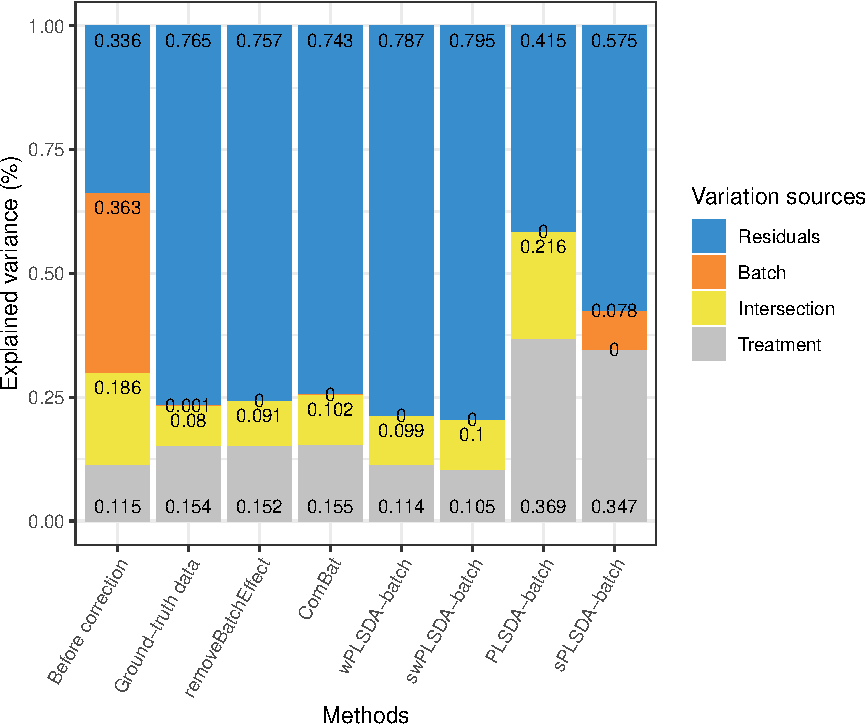
\includegraphics[width=0.7\linewidth]{PLSDAbatch_workflow_files/figure-latex/unnamed-chunk-118-1} 

}

\caption{Figure 4: Simulation studies (two batch groups): comparison of explained variance before and after batch effect correction for the unbalanced batch × treatment design.}\label{fig:unnamed-chunk-118}
\end{figure}

For a strong unbalanced batch \(\times\) treatment design, we observed the presence of intersectional variance explained by both batch and treatment effects, as expected. This source of variance is also present in the ground-truth data but should be smaller compared to the uncorrected data. Both unweighted PLSDA-batch and sPLSDA-batch performed poorly for such design - for PLSDA-batch the intersectional variance increased while for sPLSDA-batch the batch variance was not entirely removed. The other methods were successful in removing batch variance. removeBatchEffect and ComBat explained a proportion of variance by treatment similar to the ground-truth data, while wPLSDA-batch and swPLSDA-batch explained slightly less treatment variance.

\begin{Shaded}
\begin{Highlighting}[]
\DocumentationTok{\#\#\#\#\#\#\#\#\#\#\#\#\#\#\#\#\#\#\#\#\#\#\#\#\#\#\#\#\#\#\#\#\#\#\#\#\#\#\#\#\#\#\#\#\#\#\#\#\#\#\#\#\#\#\#\#\#\#\#\#\#\#\#\#\#\#\#\#\#\#\#\#\#\#\#\#\#\#\#}
\CommentTok{\# individual variance (R2)}
\DocumentationTok{\#\# boxplot}
\CommentTok{\# class}
\NormalTok{gclass }\OtherTok{\textless{}{-}} \FunctionTok{c}\NormalTok{(}\FunctionTok{rep}\NormalTok{(}\StringTok{\textquotesingle{}Treatment only\textquotesingle{}}\NormalTok{, p\_trt\_relevant), }
            \FunctionTok{rep}\NormalTok{(}\StringTok{\textquotesingle{}Batch only\textquotesingle{}}\NormalTok{, (p\_total }\SpecialCharTok{{-}}\NormalTok{ p\_trt\_relevant)))}
\NormalTok{gclass[}\FunctionTok{intersect}\NormalTok{(true.trt, true.batch)] }\OtherTok{=} \StringTok{\textquotesingle{}Treatment \& batch\textquotesingle{}}
\NormalTok{gclass[}\FunctionTok{setdiff}\NormalTok{(}\DecValTok{1}\SpecialCharTok{:}\NormalTok{p\_total, }\FunctionTok{union}\NormalTok{(true.trt, true.batch))] }\OtherTok{=} \StringTok{\textquotesingle{}No effect\textquotesingle{}}

\NormalTok{gclass }\OtherTok{\textless{}{-}} \FunctionTok{factor}\NormalTok{(gclass, }\AttributeTok{levels =} \FunctionTok{c}\NormalTok{(}\StringTok{\textquotesingle{}Treatment \& batch\textquotesingle{}}\NormalTok{, }
                                    \StringTok{\textquotesingle{}Treatment only\textquotesingle{}}\NormalTok{, }
                                    \StringTok{\textquotesingle{}Batch only\textquotesingle{}}\NormalTok{, }
                                    \StringTok{\textquotesingle{}No effect\textquotesingle{}}\NormalTok{))}

\NormalTok{before.r2.df.ggp }\OtherTok{\textless{}{-}} \FunctionTok{data.frame}\NormalTok{(}\AttributeTok{r2 =} \FunctionTok{c}\NormalTok{(}\FunctionTok{rowMeans}\NormalTok{(r2.trt.before), }
                                      \FunctionTok{rowMeans}\NormalTok{(r2.batch.before)), }
                               \AttributeTok{type =} \FunctionTok{as.factor}\NormalTok{(}\FunctionTok{rep}\NormalTok{(}\FunctionTok{c}\NormalTok{(}\StringTok{\textquotesingle{}Treatment\textquotesingle{}}\NormalTok{,}\StringTok{\textquotesingle{}Batch\textquotesingle{}}\NormalTok{), }
                                                    \AttributeTok{each =} \DecValTok{300}\NormalTok{)),}
                               \AttributeTok{class =} \FunctionTok{rep}\NormalTok{(gclass,}\DecValTok{2}\NormalTok{))}
\NormalTok{clean.r2.df.ggp }\OtherTok{\textless{}{-}} \FunctionTok{data.frame}\NormalTok{(}\AttributeTok{r2 =} \FunctionTok{c}\NormalTok{(}\FunctionTok{rowMeans}\NormalTok{(r2.trt.clean), }
                                     \FunctionTok{rowMeans}\NormalTok{(r2.batch.clean)), }
                              \AttributeTok{type =} \FunctionTok{as.factor}\NormalTok{(}\FunctionTok{rep}\NormalTok{(}\FunctionTok{c}\NormalTok{(}\StringTok{\textquotesingle{}Treatment\textquotesingle{}}\NormalTok{,}\StringTok{\textquotesingle{}Batch\textquotesingle{}}\NormalTok{), }
                                                   \AttributeTok{each =} \DecValTok{300}\NormalTok{)),}
                              \AttributeTok{class =} \FunctionTok{rep}\NormalTok{(gclass,}\DecValTok{2}\NormalTok{))}
\NormalTok{rbe.r2.df.ggp }\OtherTok{\textless{}{-}} \FunctionTok{data.frame}\NormalTok{(}\AttributeTok{r2 =} \FunctionTok{c}\NormalTok{(}\FunctionTok{rowMeans}\NormalTok{(r2.trt.rbe), }
                                   \FunctionTok{rowMeans}\NormalTok{(r2.batch.rbe)), }
                            \AttributeTok{type =} \FunctionTok{as.factor}\NormalTok{(}\FunctionTok{rep}\NormalTok{(}\FunctionTok{c}\NormalTok{(}\StringTok{\textquotesingle{}Treatment\textquotesingle{}}\NormalTok{,}\StringTok{\textquotesingle{}Batch\textquotesingle{}}\NormalTok{), }
                                                 \AttributeTok{each =} \DecValTok{300}\NormalTok{)),}
                            \AttributeTok{class =} \FunctionTok{rep}\NormalTok{(gclass,}\DecValTok{2}\NormalTok{))}
\NormalTok{combat.r2.df.ggp }\OtherTok{\textless{}{-}} \FunctionTok{data.frame}\NormalTok{(}\AttributeTok{r2 =} \FunctionTok{c}\NormalTok{(}\FunctionTok{rowMeans}\NormalTok{(r2.trt.combat), }
                                      \FunctionTok{rowMeans}\NormalTok{(r2.batch.combat)), }
                               \AttributeTok{type =} \FunctionTok{as.factor}\NormalTok{(}\FunctionTok{rep}\NormalTok{(}\FunctionTok{c}\NormalTok{(}\StringTok{\textquotesingle{}Treatment\textquotesingle{}}\NormalTok{,}\StringTok{\textquotesingle{}Batch\textquotesingle{}}\NormalTok{), }
                                                    \AttributeTok{each =} \DecValTok{300}\NormalTok{)),}
                               \AttributeTok{class =} \FunctionTok{rep}\NormalTok{(gclass,}\DecValTok{2}\NormalTok{))}
\NormalTok{wplsda\_batch.r2.df.ggp }\OtherTok{\textless{}{-}} 
  \FunctionTok{data.frame}\NormalTok{(}\AttributeTok{r2 =} \FunctionTok{c}\NormalTok{(}\FunctionTok{rowMeans}\NormalTok{(r2.trt.wplsdab), }
                    \FunctionTok{rowMeans}\NormalTok{(r2.batch.wplsdab)), }
             \AttributeTok{type =} \FunctionTok{as.factor}\NormalTok{(}\FunctionTok{rep}\NormalTok{(}\FunctionTok{c}\NormalTok{(}\StringTok{\textquotesingle{}Treatment\textquotesingle{}}\NormalTok{,}\StringTok{\textquotesingle{}Batch\textquotesingle{}}\NormalTok{), }
                                  \AttributeTok{each =} \DecValTok{300}\NormalTok{)),}
             \AttributeTok{class =} \FunctionTok{rep}\NormalTok{(gclass,}\DecValTok{2}\NormalTok{))}
\NormalTok{swplsda\_batch.r2.df.ggp }\OtherTok{\textless{}{-}} 
  \FunctionTok{data.frame}\NormalTok{(}\AttributeTok{r2 =} \FunctionTok{c}\NormalTok{(}\FunctionTok{rowMeans}\NormalTok{(r2.trt.swplsdab), }
                    \FunctionTok{rowMeans}\NormalTok{(r2.batch.swplsdab)), }
             \AttributeTok{type =} \FunctionTok{as.factor}\NormalTok{(}\FunctionTok{rep}\NormalTok{(}\FunctionTok{c}\NormalTok{(}\StringTok{\textquotesingle{}Treatment\textquotesingle{}}\NormalTok{,}\StringTok{\textquotesingle{}Batch\textquotesingle{}}\NormalTok{),}
                                  \AttributeTok{each =} \DecValTok{300}\NormalTok{)),}
             \AttributeTok{class =} \FunctionTok{rep}\NormalTok{(gclass,}\DecValTok{2}\NormalTok{))}

\NormalTok{all.r2.df.ggp }\OtherTok{\textless{}{-}} \FunctionTok{rbind}\NormalTok{(before.r2.df.ggp, clean.r2.df.ggp,}
\NormalTok{                       rbe.r2.df.ggp, combat.r2.df.ggp,}
\NormalTok{                       wplsda\_batch.r2.df.ggp, swplsda\_batch.r2.df.ggp)}

\NormalTok{all.r2.df.ggp}\SpecialCharTok{$}\NormalTok{methods }\OtherTok{\textless{}{-}} \FunctionTok{rep}\NormalTok{(}\FunctionTok{c}\NormalTok{(}\StringTok{\textquotesingle{}Before correction\textquotesingle{}}\NormalTok{, }
                               \StringTok{\textquotesingle{}Ground{-}truth data\textquotesingle{}}\NormalTok{, }
                               \StringTok{\textquotesingle{}removeBatchEffect\textquotesingle{}}\NormalTok{, }
                               \StringTok{\textquotesingle{}ComBat\textquotesingle{}}\NormalTok{,}
                               \StringTok{\textquotesingle{}wPLSDA{-}batch\textquotesingle{}}\NormalTok{, }
                               \StringTok{\textquotesingle{}swPLSDA{-}batch\textquotesingle{}}\NormalTok{), }\AttributeTok{each =} \DecValTok{600}\NormalTok{)}

\NormalTok{all.r2.df.ggp}\SpecialCharTok{$}\NormalTok{methods }\OtherTok{\textless{}{-}} \FunctionTok{factor}\NormalTok{(all.r2.df.ggp}\SpecialCharTok{$}\NormalTok{methods, }
                                \AttributeTok{levels =} \FunctionTok{unique}\NormalTok{(all.r2.df.ggp}\SpecialCharTok{$}\NormalTok{methods))}

\FunctionTok{ggplot}\NormalTok{(all.r2.df.ggp, }\FunctionTok{aes}\NormalTok{(}\AttributeTok{x =}\NormalTok{ type, }\AttributeTok{y =}\NormalTok{ r2, }\AttributeTok{fill =}\NormalTok{ class)) }\SpecialCharTok{+}
  \FunctionTok{geom\_boxplot}\NormalTok{(}\AttributeTok{alpha =} \FloatTok{0.80}\NormalTok{) }\SpecialCharTok{+}
  \FunctionTok{theme\_bw}\NormalTok{() }\SpecialCharTok{+} 
  \FunctionTok{theme}\NormalTok{(}\AttributeTok{text =} \FunctionTok{element\_text}\NormalTok{(}\AttributeTok{size =} \DecValTok{18}\NormalTok{),}
        \AttributeTok{axis.title.x =} \FunctionTok{element\_blank}\NormalTok{(),}
        \AttributeTok{axis.title.y =} \FunctionTok{element\_blank}\NormalTok{(),}
        \AttributeTok{panel.grid.minor.x =} \FunctionTok{element\_blank}\NormalTok{(),}
        \AttributeTok{panel.grid.major.x =} \FunctionTok{element\_blank}\NormalTok{(),}
        \AttributeTok{legend.position =} \StringTok{"right"}\NormalTok{) }\SpecialCharTok{+} \FunctionTok{facet\_grid}\NormalTok{(class }\SpecialCharTok{\textasciitilde{}}\NormalTok{ methods) }\SpecialCharTok{+} 
  \FunctionTok{scale\_fill\_manual}\NormalTok{(}\AttributeTok{values=}\FunctionTok{c}\NormalTok{(}\StringTok{\textquotesingle{}dark gray\textquotesingle{}}\NormalTok{, }\FunctionTok{color.mixo}\NormalTok{(}\DecValTok{4}\NormalTok{), }
                             \FunctionTok{color.mixo}\NormalTok{(}\DecValTok{5}\NormalTok{), }\FunctionTok{color.mixo}\NormalTok{(}\DecValTok{9}\NormalTok{)))}
\end{Highlighting}
\end{Shaded}

\begin{figure}

{\centering 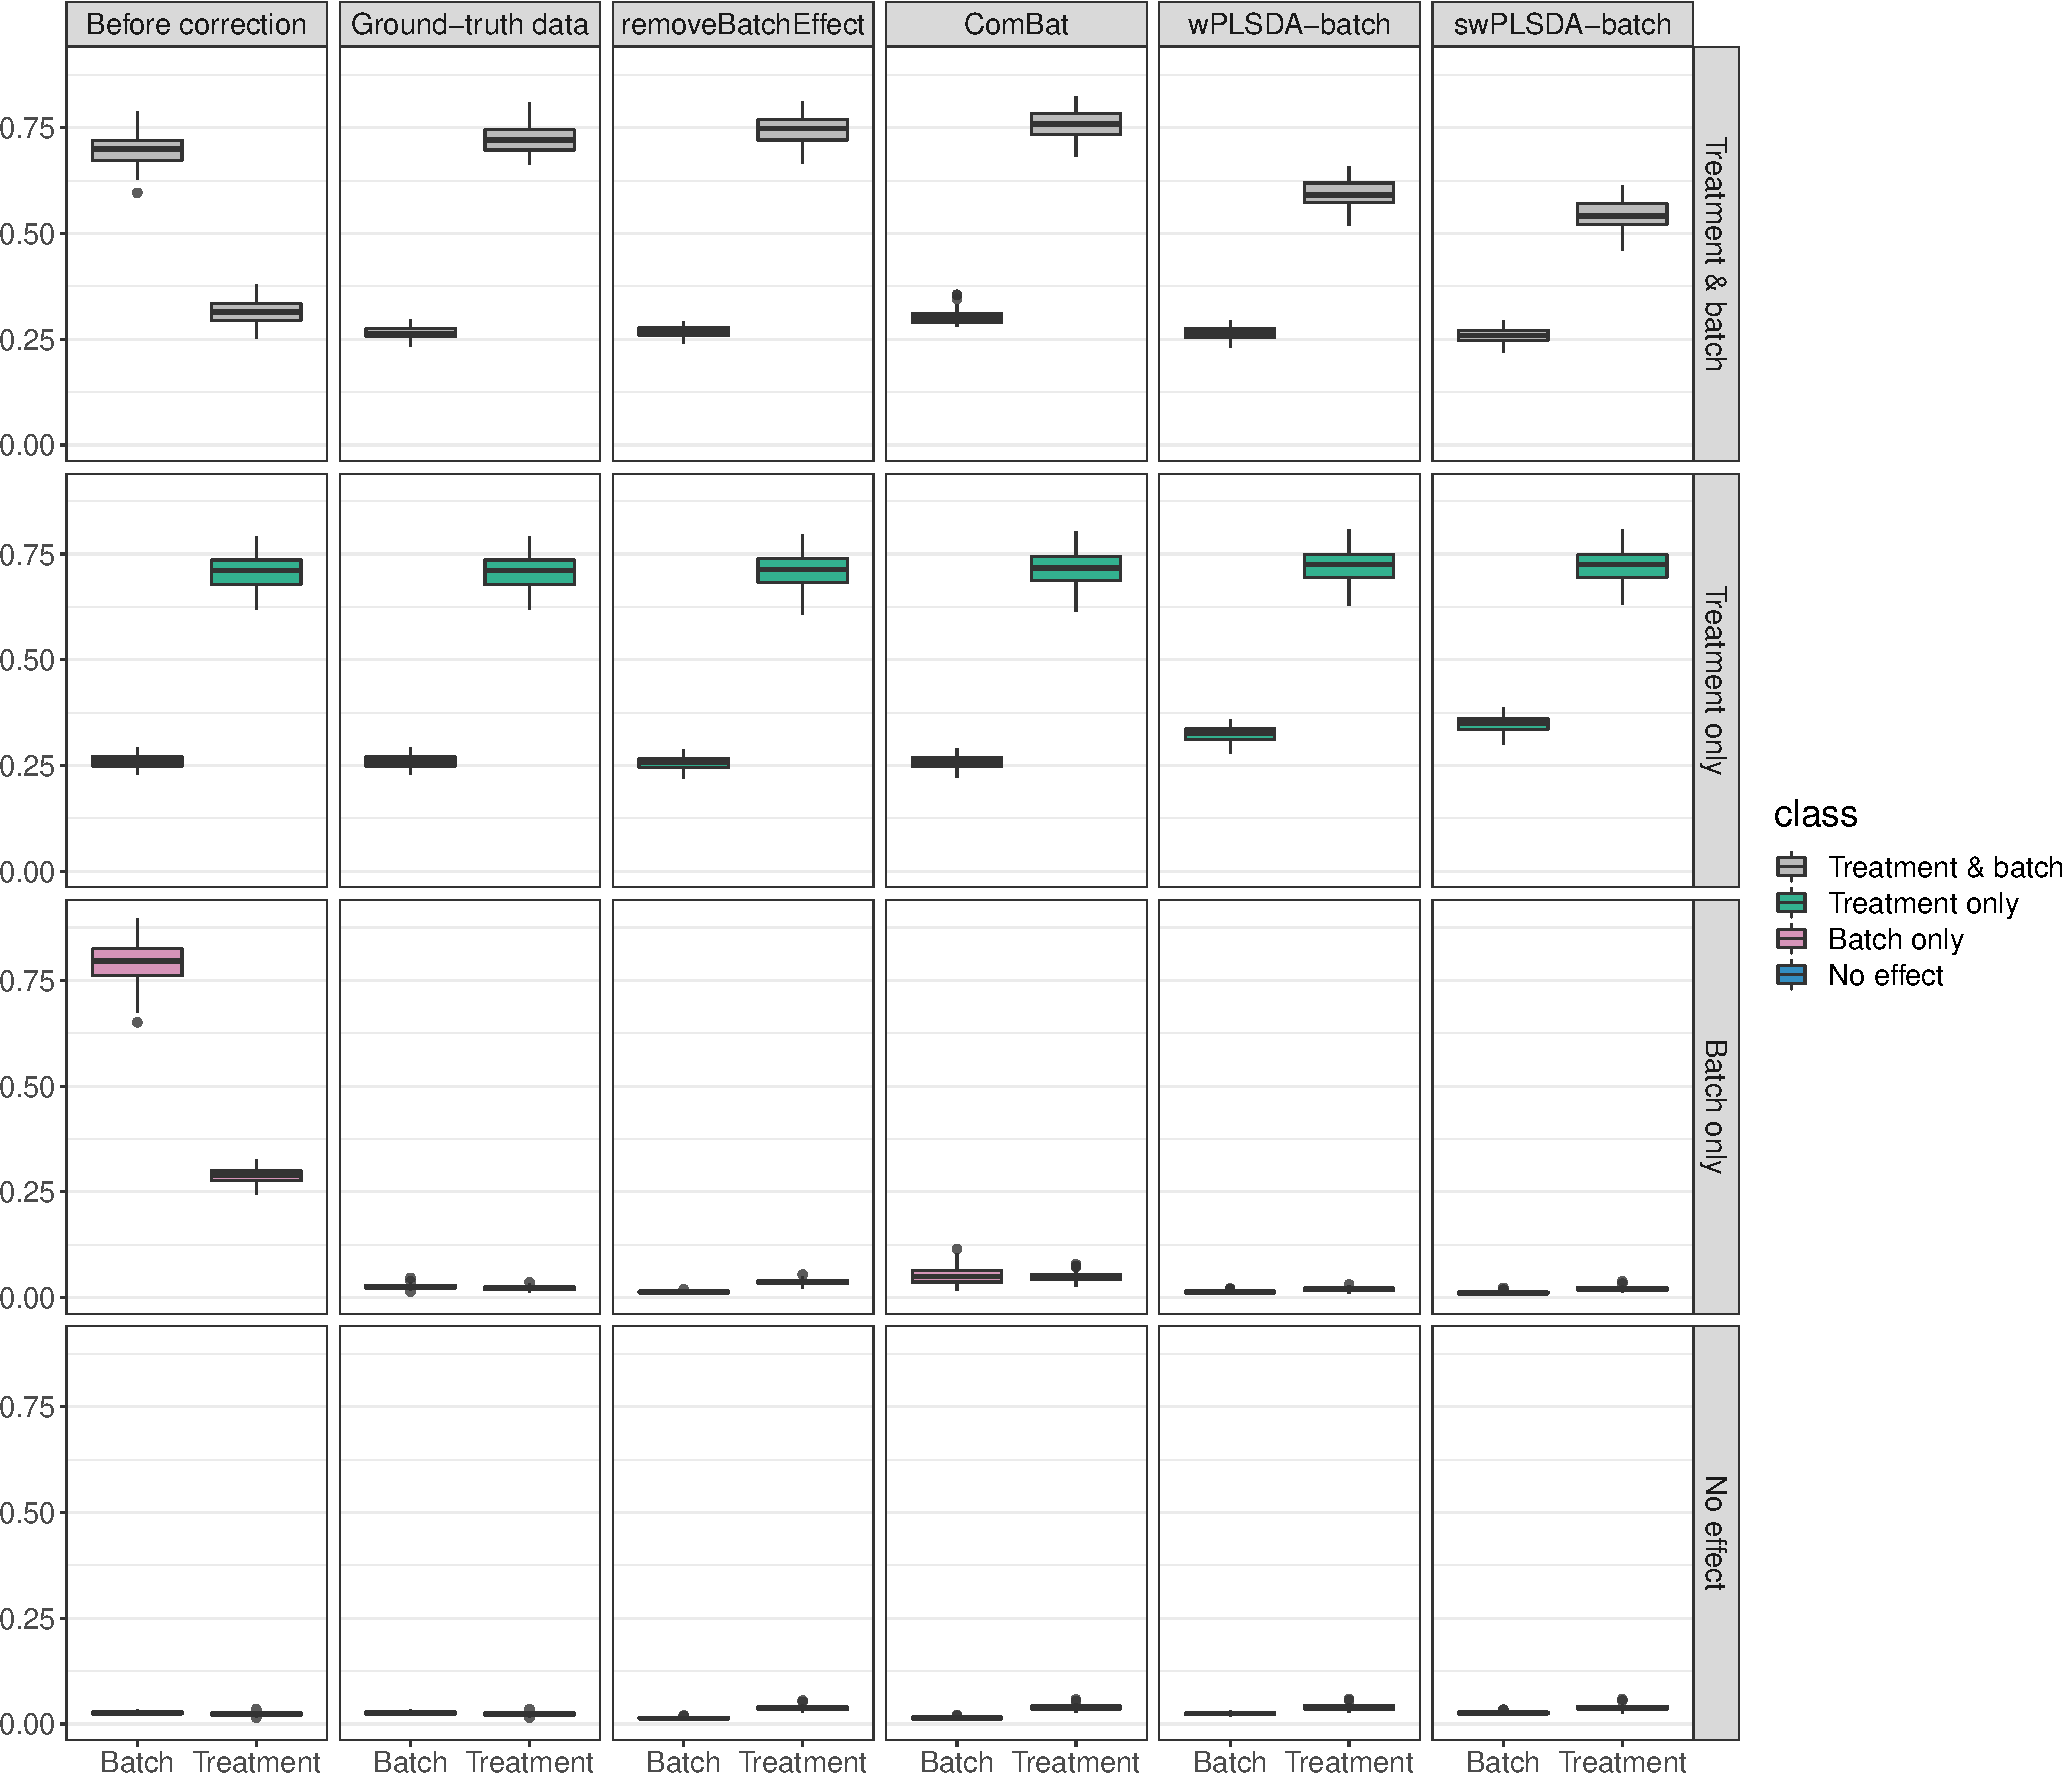
\includegraphics[width=1\linewidth]{PLSDAbatch_workflow_files/figure-latex/unnamed-chunk-119-1} 

}

\caption{Figure 5: Simulation studies (two batch groups): R2 values for each microbial variable before and after batch effect correction for the unbalanced batch × treatment design.}\label{fig:unnamed-chunk-119}
\end{figure}

\begin{Shaded}
\begin{Highlighting}[]
\DocumentationTok{\#\#\#\#\#\#\#\#\#\#\#\#\#\#\#\#\#\#\#\#\#\#\#\#\#\#\#\#\#\#\#\#\#\#\#\#\#\#\#\#\#\#\#\#\#\#\#\#\#\#\#\#\#\#\#\#\#\#\#\#\#\#\#\#\#\#\#\#\#\#\#\#\#\#\#\#\#\#\#\#}
\DocumentationTok{\#\# barplot}
\CommentTok{\# class}
\NormalTok{before.r2.df.bp }\OtherTok{\textless{}{-}} 
  \FunctionTok{data.frame}\NormalTok{(}\AttributeTok{r2 =} \FunctionTok{c}\NormalTok{(}\FunctionTok{tapply}\NormalTok{(}\FunctionTok{rowMeans}\NormalTok{(r2.trt.before), gclass, sum), }
                    \FunctionTok{tapply}\NormalTok{(}\FunctionTok{rowMeans}\NormalTok{(r2.batch.before), gclass, sum)), }
             \AttributeTok{type =} \FunctionTok{as.factor}\NormalTok{(}\FunctionTok{rep}\NormalTok{(}\FunctionTok{c}\NormalTok{(}\StringTok{\textquotesingle{}Treatment\textquotesingle{}}\NormalTok{,}\StringTok{\textquotesingle{}Batch\textquotesingle{}}\NormalTok{), }\AttributeTok{each =} \DecValTok{4}\NormalTok{)),}
             \AttributeTok{class =} \FunctionTok{factor}\NormalTok{(}\FunctionTok{rep}\NormalTok{(}\FunctionTok{levels}\NormalTok{(gclass),}\DecValTok{2}\NormalTok{), }\AttributeTok{levels =} \FunctionTok{levels}\NormalTok{(gclass)))}

\NormalTok{clean.r2.df.bp }\OtherTok{\textless{}{-}} 
  \FunctionTok{data.frame}\NormalTok{(}\AttributeTok{r2 =} \FunctionTok{c}\NormalTok{(}\FunctionTok{tapply}\NormalTok{(}\FunctionTok{rowMeans}\NormalTok{(r2.trt.clean), gclass, sum), }
                    \FunctionTok{tapply}\NormalTok{(}\FunctionTok{rowMeans}\NormalTok{(r2.batch.clean), gclass, sum)), }
             \AttributeTok{type =} \FunctionTok{as.factor}\NormalTok{(}\FunctionTok{rep}\NormalTok{(}\FunctionTok{c}\NormalTok{(}\StringTok{\textquotesingle{}Treatment\textquotesingle{}}\NormalTok{,}\StringTok{\textquotesingle{}Batch\textquotesingle{}}\NormalTok{), }\AttributeTok{each =} \DecValTok{4}\NormalTok{)),}
             \AttributeTok{class =} \FunctionTok{factor}\NormalTok{(}\FunctionTok{rep}\NormalTok{(}\FunctionTok{levels}\NormalTok{(gclass),}\DecValTok{2}\NormalTok{), }\AttributeTok{levels =} \FunctionTok{levels}\NormalTok{(gclass)))}

\NormalTok{rbe.r2.df.bp }\OtherTok{\textless{}{-}} 
  \FunctionTok{data.frame}\NormalTok{(}\AttributeTok{r2 =} \FunctionTok{c}\NormalTok{(}\FunctionTok{tapply}\NormalTok{(}\FunctionTok{rowMeans}\NormalTok{(r2.trt.rbe), gclass, sum), }
                    \FunctionTok{tapply}\NormalTok{(}\FunctionTok{rowMeans}\NormalTok{(r2.batch.rbe), gclass, sum)), }
             \AttributeTok{type =} \FunctionTok{as.factor}\NormalTok{(}\FunctionTok{rep}\NormalTok{(}\FunctionTok{c}\NormalTok{(}\StringTok{\textquotesingle{}Treatment\textquotesingle{}}\NormalTok{,}\StringTok{\textquotesingle{}Batch\textquotesingle{}}\NormalTok{), }\AttributeTok{each =} \DecValTok{4}\NormalTok{)),}
             \AttributeTok{class =} \FunctionTok{factor}\NormalTok{(}\FunctionTok{rep}\NormalTok{(}\FunctionTok{levels}\NormalTok{(gclass),}\DecValTok{2}\NormalTok{), }\AttributeTok{levels =} \FunctionTok{levels}\NormalTok{(gclass)))}

\NormalTok{combat.r2.df.bp }\OtherTok{\textless{}{-}} 
  \FunctionTok{data.frame}\NormalTok{(}\AttributeTok{r2 =} \FunctionTok{c}\NormalTok{(}\FunctionTok{tapply}\NormalTok{(}\FunctionTok{rowMeans}\NormalTok{(r2.trt.combat), gclass, sum), }
                    \FunctionTok{tapply}\NormalTok{(}\FunctionTok{rowMeans}\NormalTok{(r2.batch.combat), gclass, sum)), }
             \AttributeTok{type =} \FunctionTok{as.factor}\NormalTok{(}\FunctionTok{rep}\NormalTok{(}\FunctionTok{c}\NormalTok{(}\StringTok{\textquotesingle{}Treatment\textquotesingle{}}\NormalTok{,}\StringTok{\textquotesingle{}Batch\textquotesingle{}}\NormalTok{), }\AttributeTok{each =} \DecValTok{4}\NormalTok{)),}
             \AttributeTok{class =} \FunctionTok{factor}\NormalTok{(}\FunctionTok{rep}\NormalTok{(}\FunctionTok{levels}\NormalTok{(gclass),}\DecValTok{2}\NormalTok{), }\AttributeTok{levels =} \FunctionTok{levels}\NormalTok{(gclass)))}

\NormalTok{wplsda\_batch.r2.df.bp }\OtherTok{\textless{}{-}} 
  \FunctionTok{data.frame}\NormalTok{(}\AttributeTok{r2 =} \FunctionTok{c}\NormalTok{(}\FunctionTok{tapply}\NormalTok{(}\FunctionTok{rowMeans}\NormalTok{(r2.trt.wplsdab), gclass, sum), }
                    \FunctionTok{tapply}\NormalTok{(}\FunctionTok{rowMeans}\NormalTok{(r2.batch.wplsdab), gclass, sum)), }
             \AttributeTok{type =} \FunctionTok{as.factor}\NormalTok{(}\FunctionTok{rep}\NormalTok{(}\FunctionTok{c}\NormalTok{(}\StringTok{\textquotesingle{}Treatment\textquotesingle{}}\NormalTok{,}\StringTok{\textquotesingle{}Batch\textquotesingle{}}\NormalTok{), }\AttributeTok{each =} \DecValTok{4}\NormalTok{)),}
             \AttributeTok{class =} \FunctionTok{factor}\NormalTok{(}\FunctionTok{rep}\NormalTok{(}\FunctionTok{levels}\NormalTok{(gclass),}\DecValTok{2}\NormalTok{), }\AttributeTok{levels =} \FunctionTok{levels}\NormalTok{(gclass)))}

\NormalTok{swplsda\_batch.r2.df.bp }\OtherTok{\textless{}{-}} 
  \FunctionTok{data.frame}\NormalTok{(}\AttributeTok{r2 =} \FunctionTok{c}\NormalTok{(}\FunctionTok{tapply}\NormalTok{(}\FunctionTok{rowMeans}\NormalTok{(r2.trt.swplsdab), gclass, sum), }
                    \FunctionTok{tapply}\NormalTok{(}\FunctionTok{rowMeans}\NormalTok{(r2.batch.swplsdab), gclass, sum)), }
             \AttributeTok{type =} \FunctionTok{as.factor}\NormalTok{(}\FunctionTok{rep}\NormalTok{(}\FunctionTok{c}\NormalTok{(}\StringTok{\textquotesingle{}Treatment\textquotesingle{}}\NormalTok{,}\StringTok{\textquotesingle{}Batch\textquotesingle{}}\NormalTok{), }\AttributeTok{each =} \DecValTok{4}\NormalTok{)),}
             \AttributeTok{class =} \FunctionTok{factor}\NormalTok{(}\FunctionTok{rep}\NormalTok{(}\FunctionTok{levels}\NormalTok{(gclass),}\DecValTok{2}\NormalTok{), }\AttributeTok{levels =} \FunctionTok{levels}\NormalTok{(gclass)))}


\NormalTok{all.r2.df.bp }\OtherTok{\textless{}{-}} \FunctionTok{rbind}\NormalTok{(before.r2.df.bp, clean.r2.df.bp,}
\NormalTok{                      rbe.r2.df.bp, combat.r2.df.bp,}
\NormalTok{                      wplsda\_batch.r2.df.bp, swplsda\_batch.r2.df.bp)}


\NormalTok{all.r2.df.bp}\SpecialCharTok{$}\NormalTok{methods }\OtherTok{\textless{}{-}} \FunctionTok{rep}\NormalTok{(}\FunctionTok{c}\NormalTok{(}\StringTok{\textquotesingle{}Before correction\textquotesingle{}}\NormalTok{, }
                              \StringTok{\textquotesingle{}Ground{-}truth data\textquotesingle{}}\NormalTok{, }
                              \StringTok{\textquotesingle{}removeBatchEffect\textquotesingle{}}\NormalTok{, }
                              \StringTok{\textquotesingle{}ComBat\textquotesingle{}}\NormalTok{,}
                              \StringTok{\textquotesingle{}wPLSDA{-}batch\textquotesingle{}}\NormalTok{, }
                              \StringTok{\textquotesingle{}swPLSDA{-}batch\textquotesingle{}}\NormalTok{), }\AttributeTok{each =} \DecValTok{8}\NormalTok{)}

\NormalTok{all.r2.df.bp}\SpecialCharTok{$}\NormalTok{methods }\OtherTok{\textless{}{-}} \FunctionTok{factor}\NormalTok{(all.r2.df.bp}\SpecialCharTok{$}\NormalTok{methods, }
                               \AttributeTok{levels =} \FunctionTok{unique}\NormalTok{(all.r2.df.bp}\SpecialCharTok{$}\NormalTok{methods))}

\FunctionTok{ggplot}\NormalTok{(all.r2.df.bp, }\FunctionTok{aes}\NormalTok{(}\AttributeTok{x =}\NormalTok{ type, }\AttributeTok{y =}\NormalTok{ r2, }\AttributeTok{fill =}\NormalTok{ class)) }\SpecialCharTok{+}
  \FunctionTok{geom\_bar}\NormalTok{(}\AttributeTok{stat=}\StringTok{"identity"}\NormalTok{) }\SpecialCharTok{+} 
  \FunctionTok{theme\_bw}\NormalTok{() }\SpecialCharTok{+} 
  \FunctionTok{theme}\NormalTok{(}\AttributeTok{text =} \FunctionTok{element\_text}\NormalTok{(}\AttributeTok{size =} \DecValTok{18}\NormalTok{),}
        \AttributeTok{axis.title.x =} \FunctionTok{element\_blank}\NormalTok{(),}
        \AttributeTok{axis.title.y =} \FunctionTok{element\_blank}\NormalTok{(),}
        \AttributeTok{panel.grid.minor.x =} \FunctionTok{element\_blank}\NormalTok{(),}
        \AttributeTok{panel.grid.major.x =} \FunctionTok{element\_blank}\NormalTok{(),}
        \AttributeTok{legend.position =} \StringTok{"right"}\NormalTok{) }\SpecialCharTok{+} \FunctionTok{facet\_grid}\NormalTok{(class }\SpecialCharTok{\textasciitilde{}}\NormalTok{ methods) }\SpecialCharTok{+} 
  \FunctionTok{scale\_fill\_manual}\NormalTok{(}\AttributeTok{values=}\FunctionTok{c}\NormalTok{(}\StringTok{\textquotesingle{}dark gray\textquotesingle{}}\NormalTok{, }\FunctionTok{color.mixo}\NormalTok{(}\DecValTok{4}\NormalTok{), }
                             \FunctionTok{color.mixo}\NormalTok{(}\DecValTok{5}\NormalTok{), }\FunctionTok{color.mixo}\NormalTok{(}\DecValTok{9}\NormalTok{)))}
\end{Highlighting}
\end{Shaded}

\begin{figure}

{\centering \includegraphics[width=1\linewidth]{PLSDAbatch_workflow_files/figure-latex/unnamed-chunk-120-1} 

}

\caption{Figure 6: Simulation studies (two batch groups): the sum of R2 values for each microbial variable before and after batch effect correction for the unbalanced batch × treatment design.}\label{fig:unnamed-chunk-120}
\end{figure}

We observed similar performance for removeBatchEffect and ComBat for the unbalanced design compared to the balanced design. With wPLSDA-batch and swPLSDA-batch, variables with both treatment and batch effects explained less treatment variance after correction, compared to the ground-truth data. However, for the other variables, wPLSDA-batch and its sparse version performed as similar as the ground-truth data.

\begin{Shaded}
\begin{Highlighting}[]
\CommentTok{\# precision \& recall \& F1 (ANOVA \& sPLSDA)}
\DocumentationTok{\#\# mean}
\NormalTok{acc\_mean }\OtherTok{\textless{}{-}} \FunctionTok{rbind}\NormalTok{(}\FunctionTok{colMeans}\NormalTok{(precision\_limma), }\FunctionTok{colMeans}\NormalTok{(recall\_limma), }
                  \FunctionTok{colMeans}\NormalTok{(F1\_limma), }\FunctionTok{c}\NormalTok{(}\FunctionTok{colMeans}\NormalTok{(auc\_splsda), }\AttributeTok{sva =} \ConstantTok{NA}\NormalTok{))}
\FunctionTok{rownames}\NormalTok{(acc\_mean) }\OtherTok{\textless{}{-}} \FunctionTok{c}\NormalTok{(}\StringTok{\textquotesingle{}Precision\textquotesingle{}}\NormalTok{, }\StringTok{\textquotesingle{}Recall\textquotesingle{}}\NormalTok{, }\StringTok{\textquotesingle{}F1\textquotesingle{}}\NormalTok{, }\StringTok{\textquotesingle{}AUC\textquotesingle{}}\NormalTok{)}
\FunctionTok{colnames}\NormalTok{(acc\_mean) }\OtherTok{\textless{}{-}} \FunctionTok{c}\NormalTok{(}\StringTok{\textquotesingle{}Before correction\textquotesingle{}}\NormalTok{, }\StringTok{\textquotesingle{}Ground{-}truth data\textquotesingle{}}\NormalTok{, }
                        \StringTok{\textquotesingle{}removeBatchEffect\textquotesingle{}}\NormalTok{, }\StringTok{\textquotesingle{}ComBat\textquotesingle{}}\NormalTok{, }
                        \StringTok{\textquotesingle{}wPLSDA{-}batch\textquotesingle{}}\NormalTok{, }\StringTok{\textquotesingle{}swPLSDA{-}batch\textquotesingle{}}\NormalTok{, }\StringTok{\textquotesingle{}SVA\textquotesingle{}}\NormalTok{)}
\NormalTok{acc\_mean }\OtherTok{\textless{}{-}} \FunctionTok{format}\NormalTok{(acc\_mean, }\AttributeTok{digits =} \DecValTok{3}\NormalTok{)}
\NormalTok{knitr}\SpecialCharTok{::}\FunctionTok{kable}\NormalTok{(acc\_mean, }\AttributeTok{caption =} \StringTok{\textquotesingle{}Table 6 Simulation studies (two batch groups): summary of accuracy measurements before and after batch effect correction for the unbalanced batch × treatment design (mean).\textquotesingle{}}\NormalTok{)}
\end{Highlighting}
\end{Shaded}

\begin{table}

\caption{\label{tab:unnamed-chunk-121}Table 6 Simulation studies (two batch groups): summary of accuracy measurements before and after batch effect correction for the unbalanced batch × treatment design (mean).}
\centering
\begin{tabular}[t]{l|l|l|l|l|l|l|l}
\hline
  & Before correction & Ground-truth data & removeBatchEffect & ComBat & wPLSDA-batch & swPLSDA-batch & SVA\\
\hline
Precision & 0.385 & 0.973 & 0.901 & 0.834 & 0.943 & 0.943 & 0.401\\
\hline
Recall & 0.825 & 0.895 & 0.910 & 0.919 & 0.888 & 0.862 & 0.918\\
\hline
F1 & 0.525 & 0.932 & 0.903 & 0.873 & 0.914 & 0.900 & 0.558\\
\hline
AUC & 0.704 & 0.967 & 0.963 & 0.962 & 0.965 & 0.954 & NA\\
\hline
\end{tabular}
\end{table}

In the unbalanced design, the precision of SVA is low and very similar to the original data, indicating that the performance of SVA heavily depends on the experimental design and is likely to overfit. This may explain the somewhat inflated results of SVA in the balanced design case. wPLSDA-batch performed best with results close to those from the ground-truth data.

\begin{Shaded}
\begin{Highlighting}[]
\DocumentationTok{\#\# sd}
\NormalTok{acc\_sd }\OtherTok{\textless{}{-}} \FunctionTok{rbind}\NormalTok{(}\FunctionTok{apply}\NormalTok{(precision\_limma, }\DecValTok{2}\NormalTok{, sd), }\FunctionTok{apply}\NormalTok{(recall\_limma, }\DecValTok{2}\NormalTok{, sd), }
                \FunctionTok{apply}\NormalTok{(F1\_limma, }\DecValTok{2}\NormalTok{, sd), }\FunctionTok{c}\NormalTok{(}\FunctionTok{apply}\NormalTok{(auc\_splsda, }\DecValTok{2}\NormalTok{, sd), }\ConstantTok{NA}\NormalTok{))}
\FunctionTok{rownames}\NormalTok{(acc\_sd) }\OtherTok{\textless{}{-}} \FunctionTok{c}\NormalTok{(}\StringTok{\textquotesingle{}Precision\textquotesingle{}}\NormalTok{, }\StringTok{\textquotesingle{}Recall\textquotesingle{}}\NormalTok{, }\StringTok{\textquotesingle{}F1\textquotesingle{}}\NormalTok{, }\StringTok{\textquotesingle{}AUC\textquotesingle{}}\NormalTok{)}
\FunctionTok{colnames}\NormalTok{(acc\_sd) }\OtherTok{\textless{}{-}} \FunctionTok{c}\NormalTok{(}\StringTok{\textquotesingle{}Before correction\textquotesingle{}}\NormalTok{, }\StringTok{\textquotesingle{}Ground{-}truth data\textquotesingle{}}\NormalTok{, }
                      \StringTok{\textquotesingle{}removeBatchEffect\textquotesingle{}}\NormalTok{, }\StringTok{\textquotesingle{}ComBat\textquotesingle{}}\NormalTok{, }
                      \StringTok{\textquotesingle{}wPLSDA{-}batch\textquotesingle{}}\NormalTok{, }\StringTok{\textquotesingle{}swPLSDA{-}batch\textquotesingle{}}\NormalTok{, }\StringTok{\textquotesingle{}SVA\textquotesingle{}}\NormalTok{)}
\NormalTok{acc\_sd }\OtherTok{\textless{}{-}} \FunctionTok{format}\NormalTok{(acc\_sd, }\AttributeTok{digits =} \DecValTok{1}\NormalTok{)}
\NormalTok{knitr}\SpecialCharTok{::}\FunctionTok{kable}\NormalTok{(acc\_sd, }\AttributeTok{caption =} \StringTok{\textquotesingle{}Table 7 Simulation studies (two batch groups): summary of accuracy measurements before and after batch effect correction for the unbalanced batch × treatment design (standard deviation).\textquotesingle{}}\NormalTok{)}
\end{Highlighting}
\end{Shaded}

\begin{table}

\caption{\label{tab:unnamed-chunk-122}Table 7 Simulation studies (two batch groups): summary of accuracy measurements before and after batch effect correction for the unbalanced batch × treatment design (standard deviation).}
\centering
\begin{tabular}[t]{l|l|l|l|l|l|l|l}
\hline
  & Before correction & Ground-truth data & removeBatchEffect & ComBat & wPLSDA-batch & swPLSDA-batch & SVA\\
\hline
Precision & 0.01 & 0.05 & 0.09 & 0.08 & 0.05 & 0.05 & 0.02\\
\hline
Recall & 0.03 & 0.03 & 0.03 & 0.03 & 0.03 & 0.03 & 0.03\\
\hline
F1 & 0.01 & 0.03 & 0.05 & 0.05 & 0.03 & 0.03 & 0.02\\
\hline
AUC & 0.06 & 0.02 & 0.02 & 0.01 & 0.01 & 0.02 & NA\\
\hline
\end{tabular}
\end{table}

\hypertarget{simulations-three-batch-groups}{%
\section{Simulations (three batch groups)}\label{simulations-three-batch-groups}}

\hypertarget{balanced-batch-times-treatment-design-2}{%
\subsection{\texorpdfstring{Balanced batch \(\times\) treatment design}{Balanced batch \textbackslash times treatment design}}\label{balanced-batch-times-treatment-design-2}}

The balanced batch \(\times\) treatment experimental design included 6 samples from three batches respectively in each treatment group.

\textbf{Table 8: Balanced batch} \(\times\) treatment design in the simulation study

\begin{longtable}[]{@{}ccc@{}}
\toprule()
& Trt1 & Trt2 \\
\midrule()
\endhead
Batch1 & 6 & 6 \\
Batch2 & 6 & 6 \\
Batch3 & 6 & 6 \\
\bottomrule()
\end{longtable}

\begin{Shaded}
\begin{Highlighting}[]
\NormalTok{nitr }\OtherTok{\textless{}{-}} \DecValTok{50}
\NormalTok{N }\OtherTok{=} \DecValTok{36}
\NormalTok{p\_total }\OtherTok{=} \DecValTok{300}
\NormalTok{p\_trt\_relevant }\OtherTok{=} \DecValTok{100} 
\NormalTok{p\_bat\_relevant }\OtherTok{=} \DecValTok{200} 

\CommentTok{\# global variance (RDA)}
\NormalTok{gvar.before }\OtherTok{\textless{}{-}}\NormalTok{ gvar.clean }\OtherTok{\textless{}{-}} 
\NormalTok{  gvar.rbe }\OtherTok{\textless{}{-}}\NormalTok{ gvar.combat }\OtherTok{\textless{}{-}} 
\NormalTok{  gvar.plsdab }\OtherTok{\textless{}{-}}\NormalTok{ gvar.splsdab }\OtherTok{\textless{}{-}} \FunctionTok{data.frame}\NormalTok{(}\AttributeTok{treatment =} \ConstantTok{NA}\NormalTok{, }\AttributeTok{batch =} \ConstantTok{NA}\NormalTok{,  }
                                            \AttributeTok{intersection =} \ConstantTok{NA}\NormalTok{, }
                                            \AttributeTok{residual =} \ConstantTok{NA}\NormalTok{)}

\CommentTok{\# individual variance (R2)}
\NormalTok{r2.trt.before }\OtherTok{\textless{}{-}}\NormalTok{ r2.trt.clean }\OtherTok{\textless{}{-}} 
\NormalTok{  r2.trt.rbe  }\OtherTok{\textless{}{-}}\NormalTok{ r2.trt.combat }\OtherTok{\textless{}{-}} 
\NormalTok{  r2.trt.plsdab }\OtherTok{\textless{}{-}}\NormalTok{ r2.trt.splsdab }\OtherTok{\textless{}{-}} \FunctionTok{data.frame}\NormalTok{(}\FunctionTok{matrix}\NormalTok{(}\ConstantTok{NA}\NormalTok{, }\AttributeTok{nrow =}\NormalTok{ p\_total, }
                                                       \AttributeTok{ncol =}\NormalTok{ nitr))}
\NormalTok{r2.batch.before }\OtherTok{\textless{}{-}}\NormalTok{ r2.batch.clean }\OtherTok{\textless{}{-}} 
\NormalTok{  r2.batch.rbe  }\OtherTok{\textless{}{-}}\NormalTok{ r2.batch.combat }\OtherTok{\textless{}{-}} 
\NormalTok{  r2.batch.plsdab }\OtherTok{\textless{}{-}}\NormalTok{ r2.batch.splsdab }\OtherTok{\textless{}{-}} \FunctionTok{data.frame}\NormalTok{(}\FunctionTok{matrix}\NormalTok{(}\ConstantTok{NA}\NormalTok{, }\AttributeTok{nrow =}\NormalTok{ p\_total, }
                                                           \AttributeTok{ncol =}\NormalTok{ nitr))}

\CommentTok{\# precision \& recall \& F1 (ANOVA)}
\NormalTok{precision\_limma }\OtherTok{\textless{}{-}}\NormalTok{ recall\_limma }\OtherTok{\textless{}{-}}\NormalTok{ F1\_limma }\OtherTok{\textless{}{-}} 
  \FunctionTok{data.frame}\NormalTok{(}\AttributeTok{before =} \ConstantTok{NA}\NormalTok{, }\AttributeTok{clean =} \ConstantTok{NA}\NormalTok{, }
             \AttributeTok{rbe =} \ConstantTok{NA}\NormalTok{, }\AttributeTok{combat =} \ConstantTok{NA}\NormalTok{, }
             \AttributeTok{plsda\_batch =} \ConstantTok{NA}\NormalTok{, }\AttributeTok{splsda\_batch =} \ConstantTok{NA}\NormalTok{, }
             \AttributeTok{sva =} \ConstantTok{NA}\NormalTok{)}

\CommentTok{\# auc (splsda)}
\NormalTok{auc\_splsda }\OtherTok{\textless{}{-}} 
  \FunctionTok{data.frame}\NormalTok{(}\AttributeTok{before =} \ConstantTok{NA}\NormalTok{, }\AttributeTok{clean =} \ConstantTok{NA}\NormalTok{, }
             \AttributeTok{rbe =} \ConstantTok{NA}\NormalTok{, }\AttributeTok{combat =} \ConstantTok{NA}\NormalTok{, }
             \AttributeTok{plsda\_batch =} \ConstantTok{NA}\NormalTok{, }\AttributeTok{splsda\_batch =} \ConstantTok{NA}\NormalTok{)}


\FunctionTok{set.seed}\NormalTok{(}\DecValTok{70}\NormalTok{)}
\NormalTok{data.cor.res }\OtherTok{=} \FunctionTok{corStruct}\NormalTok{(}\AttributeTok{p =} \DecValTok{300}\NormalTok{, }\AttributeTok{zero\_prob =} \FloatTok{0.7}\NormalTok{)}

\ControlFlowTok{for}\NormalTok{(i }\ControlFlowTok{in} \DecValTok{1}\SpecialCharTok{:}\NormalTok{ nitr)\{}
  \DocumentationTok{\#\#\# initial setup }\AlertTok{\#\#\#}
\NormalTok{  simulation }\OtherTok{\textless{}{-}} \FunctionTok{simData\_mnegbinom}\NormalTok{(}\AttributeTok{batch.group =} \DecValTok{3}\NormalTok{,}
                                  \AttributeTok{mean.batch =} \DecValTok{7}\NormalTok{, }
                                  \AttributeTok{sd.batch =} \DecValTok{8}\NormalTok{, }
                                  \AttributeTok{mean.trt =} \DecValTok{3}\NormalTok{, }
                                  \AttributeTok{sd.trt =} \DecValTok{2}\NormalTok{, }
                                  \AttributeTok{mean.bg =} \DecValTok{0}\NormalTok{, }
                                  \AttributeTok{sd.bg =} \FloatTok{0.2}\NormalTok{, }
                                  \AttributeTok{N =} \DecValTok{36}\NormalTok{, }
                                  \AttributeTok{p\_total =} \DecValTok{300}\NormalTok{, }
                                  \AttributeTok{p\_trt\_relevant =} \DecValTok{100}\NormalTok{, }
                                  \AttributeTok{p\_bat\_relevant =} \DecValTok{200}\NormalTok{, }
                                  \AttributeTok{percentage\_overlap\_samples =} \FloatTok{0.5}\NormalTok{, }
                                  \AttributeTok{percentage\_overlap\_variables =} \FloatTok{0.5}\NormalTok{, }
                                  \AttributeTok{data.cor =}\NormalTok{ data.cor.res}\SpecialCharTok{$}\NormalTok{data.cor, }
                                  \AttributeTok{disp =} \DecValTok{10}\NormalTok{, }\AttributeTok{prob\_zero =} \DecValTok{0}\NormalTok{, }
                                  \AttributeTok{seeds =}\NormalTok{ i)}
  
  \FunctionTok{set.seed}\NormalTok{(i)}
\NormalTok{  raw\_count }\OtherTok{\textless{}{-}}\NormalTok{ simulation}\SpecialCharTok{$}\NormalTok{data}
\NormalTok{  raw\_count\_clean }\OtherTok{\textless{}{-}}\NormalTok{ simulation}\SpecialCharTok{$}\NormalTok{cleanData}
  
  \DocumentationTok{\#\# log transformation}
\NormalTok{  data\_log }\OtherTok{\textless{}{-}} \FunctionTok{log}\NormalTok{(raw\_count }\SpecialCharTok{+} \DecValTok{1}\NormalTok{)}
\NormalTok{  data\_log\_clean }\OtherTok{\textless{}{-}} \FunctionTok{log}\NormalTok{(raw\_count\_clean }\SpecialCharTok{+} \DecValTok{1}\NormalTok{)}
  
\NormalTok{  trt }\OtherTok{\textless{}{-}}\NormalTok{ simulation}\SpecialCharTok{$}\NormalTok{Y.trt}
\NormalTok{  batch }\OtherTok{\textless{}{-}}\NormalTok{ simulation}\SpecialCharTok{$}\NormalTok{Y.bat}
  
\NormalTok{  true.trt }\OtherTok{\textless{}{-}}\NormalTok{ simulation}\SpecialCharTok{$}\NormalTok{true.trt}
\NormalTok{  true.batch }\OtherTok{\textless{}{-}}\NormalTok{ simulation}\SpecialCharTok{$}\NormalTok{true.batch}
  
\NormalTok{  Batch\_Trt.factors }\OtherTok{\textless{}{-}} \FunctionTok{data.frame}\NormalTok{(}\AttributeTok{Batch =}\NormalTok{ batch, }\AttributeTok{Treatment =}\NormalTok{ trt)}
  
  \DocumentationTok{\#\#\# Original }\AlertTok{\#\#\#}
\NormalTok{  X }\OtherTok{\textless{}{-}}\NormalTok{ data\_log}
  
  \DocumentationTok{\#\#\# Clean data }\AlertTok{\#\#\#}
\NormalTok{  X.clean }\OtherTok{\textless{}{-}}\NormalTok{ data\_log\_clean}
  
  \DocumentationTok{\#\#\#\#\#}
  \FunctionTok{rownames}\NormalTok{(X) }\OtherTok{=} \FunctionTok{rownames}\NormalTok{(X.clean) }\OtherTok{=} \FunctionTok{names}\NormalTok{(trt) }\OtherTok{=} \FunctionTok{names}\NormalTok{(batch) }\OtherTok{=} 
    \FunctionTok{paste0}\NormalTok{(}\StringTok{\textquotesingle{}sample\textquotesingle{}}\NormalTok{, }\DecValTok{1}\SpecialCharTok{:}\NormalTok{N)}
  
  \FunctionTok{colnames}\NormalTok{(X) }\OtherTok{=} \FunctionTok{colnames}\NormalTok{(X.clean) }\OtherTok{=} \FunctionTok{paste0}\NormalTok{(}\StringTok{\textquotesingle{}otu\textquotesingle{}}\NormalTok{, }\DecValTok{1}\SpecialCharTok{:}\NormalTok{p\_total)}
  
  \DocumentationTok{\#\#\# Before correction }\AlertTok{\#\#\#}
  \CommentTok{\# global variance (RDA)}
\NormalTok{  rda.before }\OtherTok{=} \FunctionTok{varpart}\NormalTok{(}\FunctionTok{scale}\NormalTok{(X), }\SpecialCharTok{\textasciitilde{}}\NormalTok{ Treatment, }\SpecialCharTok{\textasciitilde{}}\NormalTok{ Batch, }
                       \AttributeTok{data =}\NormalTok{ Batch\_Trt.factors)}
\NormalTok{  gvar.before[i,] }\OtherTok{\textless{}{-}}\NormalTok{ rda.before}\SpecialCharTok{$}\NormalTok{part}\SpecialCharTok{$}\NormalTok{indfract}\SpecialCharTok{$}\NormalTok{Adj.R.squared}
  
  \CommentTok{\# precision \& recall \& F1 (ANOVA)}
\NormalTok{  fit.before }\OtherTok{\textless{}{-}} \FunctionTok{lmFit}\NormalTok{(}\FunctionTok{t}\NormalTok{(}\FunctionTok{scale}\NormalTok{(X)), }\AttributeTok{design =} \FunctionTok{model.matrix}\NormalTok{(}\SpecialCharTok{\textasciitilde{}} \FunctionTok{as.factor}\NormalTok{(trt)))}
\NormalTok{  fit.result.before }\OtherTok{\textless{}{-}} \FunctionTok{topTable}\NormalTok{(}\FunctionTok{eBayes}\NormalTok{(fit.before), }\AttributeTok{coef =} \DecValTok{2}\NormalTok{, }\AttributeTok{number =}\NormalTok{ p\_total)}
\NormalTok{  otu.sig.before }\OtherTok{\textless{}{-}} 
    \FunctionTok{rownames}\NormalTok{(fit.result.before)[fit.result.before}\SpecialCharTok{$}\NormalTok{adj.P.Val }\SpecialCharTok{\textless{}=} \FloatTok{0.05}\NormalTok{]}
  
\NormalTok{  precision\_limma.before }\OtherTok{\textless{}{-}} 
    \FunctionTok{length}\NormalTok{(}\FunctionTok{intersect}\NormalTok{(}\FunctionTok{colnames}\NormalTok{(X)[true.trt], otu.sig.before))}\SpecialCharTok{/}
    \FunctionTok{length}\NormalTok{(otu.sig.before)}
\NormalTok{  recall\_limma.before }\OtherTok{\textless{}{-}} 
    \FunctionTok{length}\NormalTok{(}\FunctionTok{intersect}\NormalTok{(}\FunctionTok{colnames}\NormalTok{(X)[true.trt], otu.sig.before))}\SpecialCharTok{/}\FunctionTok{length}\NormalTok{(true.trt)}
\NormalTok{  F1\_limma.before }\OtherTok{\textless{}{-}} 
\NormalTok{    (}\DecValTok{2}\SpecialCharTok{*}\NormalTok{precision\_limma.before}\SpecialCharTok{*}\NormalTok{recall\_limma.before)}\SpecialCharTok{/}
\NormalTok{    (precision\_limma.before }\SpecialCharTok{+}\NormalTok{ recall\_limma.before)}
  
  \DocumentationTok{\#\# replace NA value with 0}
  \ControlFlowTok{if}\NormalTok{(precision\_limma.before }\SpecialCharTok{==} \StringTok{\textquotesingle{}NaN\textquotesingle{}}\NormalTok{)\{}
\NormalTok{    precision\_limma.before }\OtherTok{=} \DecValTok{0}
\NormalTok{  \}}
  \ControlFlowTok{if}\NormalTok{(F1\_limma.before }\SpecialCharTok{==} \StringTok{\textquotesingle{}NaN\textquotesingle{}}\NormalTok{)\{}
\NormalTok{    F1\_limma.before }\OtherTok{=} \DecValTok{0}
\NormalTok{  \}}
  
  \CommentTok{\# individual variance (R2)}
\NormalTok{  indiv.trt.before }\OtherTok{\textless{}{-}} \FunctionTok{c}\NormalTok{()}
\NormalTok{  indiv.batch.before }\OtherTok{\textless{}{-}} \FunctionTok{c}\NormalTok{()}
  \ControlFlowTok{for}\NormalTok{(c }\ControlFlowTok{in} \FunctionTok{seq\_len}\NormalTok{(}\FunctionTok{ncol}\NormalTok{(X)))\{}
\NormalTok{    fit.res1 }\OtherTok{\textless{}{-}} \FunctionTok{lm}\NormalTok{(}\FunctionTok{scale}\NormalTok{(X)[ ,c] }\SpecialCharTok{\textasciitilde{}}\NormalTok{ trt)}
\NormalTok{    fit.summary1 }\OtherTok{\textless{}{-}} \FunctionTok{summary}\NormalTok{(fit.res1)}
\NormalTok{    fit.res2 }\OtherTok{\textless{}{-}} \FunctionTok{lm}\NormalTok{(}\FunctionTok{scale}\NormalTok{(X)[ ,c] }\SpecialCharTok{\textasciitilde{}}\NormalTok{ batch)}
\NormalTok{    fit.summary2 }\OtherTok{\textless{}{-}} \FunctionTok{summary}\NormalTok{(fit.res2)}
\NormalTok{    indiv.trt.before }\OtherTok{\textless{}{-}} \FunctionTok{c}\NormalTok{(indiv.trt.before, fit.summary1}\SpecialCharTok{$}\NormalTok{r.squared)}
\NormalTok{    indiv.batch.before }\OtherTok{\textless{}{-}} \FunctionTok{c}\NormalTok{(indiv.batch.before, fit.summary2}\SpecialCharTok{$}\NormalTok{r.squared)}
\NormalTok{  \}}
\NormalTok{  r2.trt.before[ ,i] }\OtherTok{\textless{}{-}}\NormalTok{  indiv.trt.before}
\NormalTok{  r2.batch.before[ ,i] }\OtherTok{\textless{}{-}}\NormalTok{  indiv.batch.before}
  
  
  \CommentTok{\# auc (sPLSDA)}
\NormalTok{  fit.before\_plsda }\OtherTok{\textless{}{-}} \FunctionTok{splsda}\NormalTok{(}\AttributeTok{X =}\NormalTok{ X, }\AttributeTok{Y =}\NormalTok{ trt, }\AttributeTok{ncomp =} \DecValTok{1}\NormalTok{)}
  
\NormalTok{  true.response }\OtherTok{\textless{}{-}} \FunctionTok{rep}\NormalTok{(}\DecValTok{0}\NormalTok{, p\_total)}
\NormalTok{  true.response[true.trt] }\OtherTok{=} \DecValTok{1}
\NormalTok{  before.predictor }\OtherTok{\textless{}{-}} \FunctionTok{as.numeric}\NormalTok{(}\FunctionTok{abs}\NormalTok{(fit.before\_plsda}\SpecialCharTok{$}\NormalTok{loadings}\SpecialCharTok{$}\NormalTok{X))}
\NormalTok{  roc.before\_splsda }\OtherTok{\textless{}{-}} \FunctionTok{roc}\NormalTok{(true.response, before.predictor, }\AttributeTok{auc =} \ConstantTok{TRUE}\NormalTok{)}
\NormalTok{  auc.before\_splsda }\OtherTok{\textless{}{-}}\NormalTok{ roc.before\_splsda}\SpecialCharTok{$}\NormalTok{auc}
  
  
  \DocumentationTok{\#\#\#\#\#\#\#\#\#\#\#\#\#\#\#\#\#\#\#\#\#\#\#\#\#\#\#\#\#\#\#\#\#\#\#\#\#\#\#\#\#\#\#\#\#\#\#\#\#\#\#\#\#\#\#\#\#\#\#\#\#\#\#\#\#\#\#\#\#\#\#\#\#\#\#\#\#\#}
  \DocumentationTok{\#\#\# Ground{-}truth data }\AlertTok{\#\#\#}
  \CommentTok{\# global variance (RDA)}
\NormalTok{  rda.clean }\OtherTok{=} \FunctionTok{varpart}\NormalTok{(}\FunctionTok{scale}\NormalTok{(X.clean), }\SpecialCharTok{\textasciitilde{}}\NormalTok{ Treatment, }\SpecialCharTok{\textasciitilde{}}\NormalTok{ Batch, }
                      \AttributeTok{data =}\NormalTok{ Batch\_Trt.factors)}
\NormalTok{  gvar.clean[i, ] }\OtherTok{\textless{}{-}}\NormalTok{ rda.clean}\SpecialCharTok{$}\NormalTok{part}\SpecialCharTok{$}\NormalTok{indfract}\SpecialCharTok{$}\NormalTok{Adj.R.squared}
  
  
  \CommentTok{\# precision \& recall \& F1 (ANOVA)}
\NormalTok{  fit.clean }\OtherTok{\textless{}{-}} \FunctionTok{lmFit}\NormalTok{(}\FunctionTok{t}\NormalTok{(}\FunctionTok{scale}\NormalTok{(X.clean)), }\AttributeTok{design =} \FunctionTok{model.matrix}\NormalTok{(}\SpecialCharTok{\textasciitilde{}} \FunctionTok{as.factor}\NormalTok{(trt)))}
\NormalTok{  fit.result.clean }\OtherTok{\textless{}{-}} \FunctionTok{topTable}\NormalTok{(}\FunctionTok{eBayes}\NormalTok{(fit.clean), }\AttributeTok{coef =} \DecValTok{2}\NormalTok{, }\AttributeTok{number =}\NormalTok{ p\_total)}
\NormalTok{  otu.sig.clean }\OtherTok{\textless{}{-}} 
    \FunctionTok{rownames}\NormalTok{(fit.result.clean)[fit.result.clean}\SpecialCharTok{$}\NormalTok{adj.P.Val }\SpecialCharTok{\textless{}=} \FloatTok{0.05}\NormalTok{]}
  
\NormalTok{  precision\_limma.clean }\OtherTok{\textless{}{-}} 
    \FunctionTok{length}\NormalTok{(}\FunctionTok{intersect}\NormalTok{(}\FunctionTok{colnames}\NormalTok{(X)[true.trt], otu.sig.clean))}\SpecialCharTok{/}
    \FunctionTok{length}\NormalTok{(otu.sig.clean)}
\NormalTok{  recall\_limma.clean}\OtherTok{\textless{}{-}} 
    \FunctionTok{length}\NormalTok{(}\FunctionTok{intersect}\NormalTok{(}\FunctionTok{colnames}\NormalTok{(X)[true.trt], otu.sig.clean))}\SpecialCharTok{/}\FunctionTok{length}\NormalTok{(true.trt)}
\NormalTok{  F1\_limma.clean }\OtherTok{\textless{}{-}} 
\NormalTok{    (}\DecValTok{2}\SpecialCharTok{*}\NormalTok{precision\_limma.clean}\SpecialCharTok{*}\NormalTok{recall\_limma.clean)}\SpecialCharTok{/}
\NormalTok{    (precision\_limma.clean }\SpecialCharTok{+}\NormalTok{ recall\_limma.clean)}
  
  \DocumentationTok{\#\# replace NA value with 0}
  \ControlFlowTok{if}\NormalTok{(precision\_limma.clean }\SpecialCharTok{==} \StringTok{\textquotesingle{}NaN\textquotesingle{}}\NormalTok{)\{}
\NormalTok{    precision\_limma.clean }\OtherTok{=} \DecValTok{0}
\NormalTok{  \}}
  \ControlFlowTok{if}\NormalTok{(F1\_limma.clean }\SpecialCharTok{==} \StringTok{\textquotesingle{}NaN\textquotesingle{}}\NormalTok{)\{}
\NormalTok{    F1\_limma.clean }\OtherTok{=} \DecValTok{0}
\NormalTok{  \}}
  
  \CommentTok{\# individual variance (R2)}
\NormalTok{  indiv.trt.clean }\OtherTok{\textless{}{-}} \FunctionTok{c}\NormalTok{()}
\NormalTok{  indiv.batch.clean }\OtherTok{\textless{}{-}} \FunctionTok{c}\NormalTok{()}
  \ControlFlowTok{for}\NormalTok{(c }\ControlFlowTok{in} \FunctionTok{seq\_len}\NormalTok{(}\FunctionTok{ncol}\NormalTok{(X.clean)))\{}
\NormalTok{    fit.res1 }\OtherTok{\textless{}{-}} \FunctionTok{lm}\NormalTok{(}\FunctionTok{scale}\NormalTok{(X.clean)[ ,c] }\SpecialCharTok{\textasciitilde{}}\NormalTok{ trt)}
\NormalTok{    fit.summary1 }\OtherTok{\textless{}{-}} \FunctionTok{summary}\NormalTok{(fit.res1)}
\NormalTok{    fit.res2 }\OtherTok{\textless{}{-}} \FunctionTok{lm}\NormalTok{(}\FunctionTok{scale}\NormalTok{(X.clean)[ ,c] }\SpecialCharTok{\textasciitilde{}}\NormalTok{ batch)}
\NormalTok{    fit.summary2 }\OtherTok{\textless{}{-}} \FunctionTok{summary}\NormalTok{(fit.res2)}
\NormalTok{    indiv.trt.clean }\OtherTok{\textless{}{-}} \FunctionTok{c}\NormalTok{(indiv.trt.clean, fit.summary1}\SpecialCharTok{$}\NormalTok{r.squared)}
\NormalTok{    indiv.batch.clean }\OtherTok{\textless{}{-}} \FunctionTok{c}\NormalTok{(indiv.batch.clean, fit.summary2}\SpecialCharTok{$}\NormalTok{r.squared)}
\NormalTok{  \}}
\NormalTok{  r2.trt.clean[ ,i] }\OtherTok{\textless{}{-}}\NormalTok{  indiv.trt.clean}
\NormalTok{  r2.batch.clean[ ,i] }\OtherTok{\textless{}{-}}\NormalTok{  indiv.batch.clean}
  
  \CommentTok{\# auc (sPLSDA)}
\NormalTok{  fit.clean\_plsda }\OtherTok{\textless{}{-}} \FunctionTok{splsda}\NormalTok{(}\AttributeTok{X =}\NormalTok{ X.clean, }\AttributeTok{Y =}\NormalTok{ trt, }\AttributeTok{ncomp =} \DecValTok{1}\NormalTok{)}
  
\NormalTok{  clean.predictor }\OtherTok{\textless{}{-}} \FunctionTok{as.numeric}\NormalTok{(}\FunctionTok{abs}\NormalTok{(fit.clean\_plsda}\SpecialCharTok{$}\NormalTok{loadings}\SpecialCharTok{$}\NormalTok{X))}
\NormalTok{  roc.clean\_splsda }\OtherTok{\textless{}{-}} \FunctionTok{roc}\NormalTok{(true.response, clean.predictor, }\AttributeTok{auc =} \ConstantTok{TRUE}\NormalTok{)}
\NormalTok{  auc.clean\_splsda }\OtherTok{\textless{}{-}}\NormalTok{ roc.clean\_splsda}\SpecialCharTok{$}\NormalTok{auc}
  
  \DocumentationTok{\#\#\#\#\#\#\#\#\#\#\#\#\#\#\#\#\#\#\#\#\#\#\#\#\#\#\#\#\#\#\#\#\#\#\#\#\#\#\#\#\#\#\#\#\#\#\#\#\#\#\#\#\#\#\#\#\#\#\#\#\#\#\#\#\#\#\#\#\#\#\#\#\#\#\#\#\#\#}
  \DocumentationTok{\#\#\# removeBatchEffect corrected data }\AlertTok{\#\#\#}
\NormalTok{  X.rbe }\OtherTok{\textless{}{-}}\FunctionTok{t}\NormalTok{(}\FunctionTok{removeBatchEffect}\NormalTok{(}\FunctionTok{t}\NormalTok{(X), }\AttributeTok{batch =}\NormalTok{ batch, }
                              \AttributeTok{design =} \FunctionTok{model.matrix}\NormalTok{(}\SpecialCharTok{\textasciitilde{}} \FunctionTok{as.factor}\NormalTok{(trt))))}
  
  \CommentTok{\# global variance (RDA)}
\NormalTok{  rda.rbe }\OtherTok{=} \FunctionTok{varpart}\NormalTok{(}\FunctionTok{scale}\NormalTok{(X.rbe), }\SpecialCharTok{\textasciitilde{}}\NormalTok{ Treatment, }\SpecialCharTok{\textasciitilde{}}\NormalTok{ Batch, }
                    \AttributeTok{data =}\NormalTok{ Batch\_Trt.factors)}
\NormalTok{  gvar.rbe[i, ] }\OtherTok{\textless{}{-}}\NormalTok{ rda.rbe}\SpecialCharTok{$}\NormalTok{part}\SpecialCharTok{$}\NormalTok{indfract}\SpecialCharTok{$}\NormalTok{Adj.R.squared}
  
  \CommentTok{\# precision \& recall \& F1 (ANOVA)}
\NormalTok{  fit.rbe }\OtherTok{\textless{}{-}} \FunctionTok{lmFit}\NormalTok{(}\FunctionTok{t}\NormalTok{(}\FunctionTok{scale}\NormalTok{(X.rbe)), }
                   \AttributeTok{design =} \FunctionTok{model.matrix}\NormalTok{( }\SpecialCharTok{\textasciitilde{}} \FunctionTok{as.factor}\NormalTok{(trt)))}
\NormalTok{  fit.result.rbe }\OtherTok{\textless{}{-}} \FunctionTok{topTable}\NormalTok{(}\FunctionTok{eBayes}\NormalTok{(fit.rbe), }\AttributeTok{coef =} \DecValTok{2}\NormalTok{, }\AttributeTok{number =}\NormalTok{ p\_total)}
\NormalTok{  otu.sig.rbe }\OtherTok{\textless{}{-}} \FunctionTok{rownames}\NormalTok{(fit.result.rbe)[fit.result.rbe}\SpecialCharTok{$}\NormalTok{adj.P.Val }\SpecialCharTok{\textless{}=} \FloatTok{0.05}\NormalTok{]}
  
\NormalTok{  precision\_limma.rbe }\OtherTok{\textless{}{-}} \FunctionTok{length}\NormalTok{(}\FunctionTok{intersect}\NormalTok{(}\FunctionTok{colnames}\NormalTok{(X)[true.trt], otu.sig.rbe))}\SpecialCharTok{/}
    \FunctionTok{length}\NormalTok{(otu.sig.rbe)}
\NormalTok{  recall\_limma.rbe }\OtherTok{\textless{}{-}} \FunctionTok{length}\NormalTok{(}\FunctionTok{intersect}\NormalTok{(}\FunctionTok{colnames}\NormalTok{(X)[true.trt], otu.sig.rbe))}\SpecialCharTok{/}
    \FunctionTok{length}\NormalTok{(true.trt)}
\NormalTok{  F1\_limma.rbe }\OtherTok{\textless{}{-}}\NormalTok{ (}\DecValTok{2}\SpecialCharTok{*}\NormalTok{precision\_limma.rbe}\SpecialCharTok{*}\NormalTok{recall\_limma.rbe)}\SpecialCharTok{/}
\NormalTok{    (precision\_limma.rbe }\SpecialCharTok{+}\NormalTok{ recall\_limma.rbe)}
  
  \DocumentationTok{\#\# replace NA value with 0}
  \ControlFlowTok{if}\NormalTok{(precision\_limma.rbe }\SpecialCharTok{==} \StringTok{\textquotesingle{}NaN\textquotesingle{}}\NormalTok{)\{}
\NormalTok{    precision\_limma.rbe }\OtherTok{=} \DecValTok{0}
\NormalTok{  \}}
  \ControlFlowTok{if}\NormalTok{(F1\_limma.rbe }\SpecialCharTok{==} \StringTok{\textquotesingle{}NaN\textquotesingle{}}\NormalTok{)\{}
\NormalTok{    F1\_limma.rbe }\OtherTok{=} \DecValTok{0}
\NormalTok{  \}}
  
  \CommentTok{\# individual variance (R2)}
\NormalTok{  indiv.trt.rbe }\OtherTok{\textless{}{-}} \FunctionTok{c}\NormalTok{()}
\NormalTok{  indiv.batch.rbe }\OtherTok{\textless{}{-}} \FunctionTok{c}\NormalTok{()}
  \ControlFlowTok{for}\NormalTok{(c }\ControlFlowTok{in} \FunctionTok{seq\_len}\NormalTok{(}\FunctionTok{ncol}\NormalTok{(X.rbe)))\{}
\NormalTok{    fit.res1 }\OtherTok{\textless{}{-}} \FunctionTok{lm}\NormalTok{(}\FunctionTok{scale}\NormalTok{(X.rbe)[ ,c] }\SpecialCharTok{\textasciitilde{}}\NormalTok{ trt)}
\NormalTok{    fit.summary1 }\OtherTok{\textless{}{-}} \FunctionTok{summary}\NormalTok{(fit.res1)}
\NormalTok{    fit.res2 }\OtherTok{\textless{}{-}} \FunctionTok{lm}\NormalTok{(}\FunctionTok{scale}\NormalTok{(X.rbe)[ ,c] }\SpecialCharTok{\textasciitilde{}}\NormalTok{ batch)}
\NormalTok{    fit.summary2 }\OtherTok{\textless{}{-}} \FunctionTok{summary}\NormalTok{(fit.res2)}
\NormalTok{    indiv.trt.rbe }\OtherTok{\textless{}{-}} \FunctionTok{c}\NormalTok{(indiv.trt.rbe, fit.summary1}\SpecialCharTok{$}\NormalTok{r.squared)}
\NormalTok{    indiv.batch.rbe }\OtherTok{\textless{}{-}} \FunctionTok{c}\NormalTok{(indiv.batch.rbe, fit.summary2}\SpecialCharTok{$}\NormalTok{r.squared)}
\NormalTok{  \}}
\NormalTok{  r2.trt.rbe[ ,i] }\OtherTok{\textless{}{-}}\NormalTok{  indiv.trt.rbe}
\NormalTok{  r2.batch.rbe[ ,i] }\OtherTok{\textless{}{-}}\NormalTok{  indiv.batch.rbe}
  
  
  \CommentTok{\# auc (sPLSDA)}
\NormalTok{  fit.rbe\_plsda }\OtherTok{\textless{}{-}} \FunctionTok{splsda}\NormalTok{(}\AttributeTok{X =}\NormalTok{ X.rbe, }\AttributeTok{Y =}\NormalTok{ trt, }\AttributeTok{ncomp =} \DecValTok{1}\NormalTok{)}
  
\NormalTok{  rbe.predictor }\OtherTok{\textless{}{-}} \FunctionTok{as.numeric}\NormalTok{(}\FunctionTok{abs}\NormalTok{(fit.rbe\_plsda}\SpecialCharTok{$}\NormalTok{loadings}\SpecialCharTok{$}\NormalTok{X))}
\NormalTok{  roc.rbe\_splsda }\OtherTok{\textless{}{-}} \FunctionTok{roc}\NormalTok{(true.response, rbe.predictor, }\AttributeTok{auc =} \ConstantTok{TRUE}\NormalTok{)}
\NormalTok{  auc.rbe\_splsda }\OtherTok{\textless{}{-}}\NormalTok{ roc.rbe\_splsda}\SpecialCharTok{$}\NormalTok{auc}
  
  \DocumentationTok{\#\#\#\#\#\#\#\#\#\#\#\#\#\#\#\#\#\#\#\#\#\#\#\#\#\#\#\#\#\#\#\#\#\#\#\#\#\#\#\#\#\#\#\#\#\#\#\#\#\#\#\#\#\#\#\#\#\#\#\#\#\#\#\#\#\#\#\#\#\#\#\#\#\#\#\#\#\#}
  \DocumentationTok{\#\#\# ComBat corrected data }\AlertTok{\#\#\#}
\NormalTok{  X.combat }\OtherTok{\textless{}{-}} \FunctionTok{t}\NormalTok{(}\FunctionTok{ComBat}\NormalTok{(}\AttributeTok{dat =} \FunctionTok{t}\NormalTok{(X), }\AttributeTok{batch =}\NormalTok{ batch, }
                       \AttributeTok{mod =} \FunctionTok{model.matrix}\NormalTok{( }\SpecialCharTok{\textasciitilde{}} \FunctionTok{as.factor}\NormalTok{(trt))))}
  
  \CommentTok{\# global variance (RDA)}
\NormalTok{  rda.combat }\OtherTok{=} \FunctionTok{varpart}\NormalTok{(}\FunctionTok{scale}\NormalTok{(X.combat), }\SpecialCharTok{\textasciitilde{}}\NormalTok{ Treatment, }\SpecialCharTok{\textasciitilde{}}\NormalTok{ Batch, }
                       \AttributeTok{data =}\NormalTok{ Batch\_Trt.factors)}
\NormalTok{  gvar.combat[i, ] }\OtherTok{\textless{}{-}}\NormalTok{ rda.combat}\SpecialCharTok{$}\NormalTok{part}\SpecialCharTok{$}\NormalTok{indfract}\SpecialCharTok{$}\NormalTok{Adj.R.squared}
  
  \CommentTok{\# precision \& recall \& F1 (ANOVA)}
\NormalTok{  fit.combat }\OtherTok{\textless{}{-}} \FunctionTok{lmFit}\NormalTok{(}\FunctionTok{t}\NormalTok{(}\FunctionTok{scale}\NormalTok{(X.combat)), }
                      \AttributeTok{design =} \FunctionTok{model.matrix}\NormalTok{( }\SpecialCharTok{\textasciitilde{}} \FunctionTok{as.factor}\NormalTok{(trt)))}
\NormalTok{  fit.result.combat }\OtherTok{\textless{}{-}} \FunctionTok{topTable}\NormalTok{(}\FunctionTok{eBayes}\NormalTok{(fit.combat), }\AttributeTok{coef =} \DecValTok{2}\NormalTok{, }\AttributeTok{number =}\NormalTok{ p\_total)}
\NormalTok{  otu.sig.combat }\OtherTok{\textless{}{-}} \FunctionTok{rownames}\NormalTok{(fit.result.combat)[fit.result.combat}\SpecialCharTok{$}\NormalTok{adj.P.Val }\SpecialCharTok{\textless{}=} 
                                                  \FloatTok{0.05}\NormalTok{]}
  
\NormalTok{  precision\_limma.combat }\OtherTok{\textless{}{-}} 
    \FunctionTok{length}\NormalTok{(}\FunctionTok{intersect}\NormalTok{(}\FunctionTok{colnames}\NormalTok{(X)[true.trt], otu.sig.combat))}\SpecialCharTok{/}
    \FunctionTok{length}\NormalTok{(otu.sig.combat)}
\NormalTok{  recall\_limma.combat }\OtherTok{\textless{}{-}} 
    \FunctionTok{length}\NormalTok{(}\FunctionTok{intersect}\NormalTok{(}\FunctionTok{colnames}\NormalTok{(X)[true.trt], otu.sig.combat))}\SpecialCharTok{/}
    \FunctionTok{length}\NormalTok{(true.trt)}
\NormalTok{  F1\_limma.combat }\OtherTok{\textless{}{-}}\NormalTok{ (}\DecValTok{2}\SpecialCharTok{*}\NormalTok{precision\_limma.combat}\SpecialCharTok{*}\NormalTok{recall\_limma.combat)}\SpecialCharTok{/}
\NormalTok{    (precision\_limma.combat }\SpecialCharTok{+}\NormalTok{ recall\_limma.combat)}
  
  \DocumentationTok{\#\# replace NA value with 0}
  \ControlFlowTok{if}\NormalTok{(precision\_limma.combat }\SpecialCharTok{==} \StringTok{\textquotesingle{}NaN\textquotesingle{}}\NormalTok{)\{}
\NormalTok{    precision\_limma.combat }\OtherTok{=} \DecValTok{0}
\NormalTok{  \}}
  \ControlFlowTok{if}\NormalTok{(F1\_limma.combat }\SpecialCharTok{==} \StringTok{\textquotesingle{}NaN\textquotesingle{}}\NormalTok{)\{}
\NormalTok{    F1\_limma.combat }\OtherTok{=} \DecValTok{0}
\NormalTok{  \}}
  
  \CommentTok{\# individual variance (R2)}
\NormalTok{  indiv.trt.combat }\OtherTok{\textless{}{-}} \FunctionTok{c}\NormalTok{()}
\NormalTok{  indiv.batch.combat }\OtherTok{\textless{}{-}} \FunctionTok{c}\NormalTok{()}
  \ControlFlowTok{for}\NormalTok{(c }\ControlFlowTok{in} \FunctionTok{seq\_len}\NormalTok{(}\FunctionTok{ncol}\NormalTok{(X.combat)))\{}
\NormalTok{    fit.res1 }\OtherTok{\textless{}{-}} \FunctionTok{lm}\NormalTok{(}\FunctionTok{scale}\NormalTok{(X.combat)[ ,c] }\SpecialCharTok{\textasciitilde{}}\NormalTok{ trt)}
\NormalTok{    fit.summary1 }\OtherTok{\textless{}{-}} \FunctionTok{summary}\NormalTok{(fit.res1)}
\NormalTok{    fit.res2 }\OtherTok{\textless{}{-}} \FunctionTok{lm}\NormalTok{(}\FunctionTok{scale}\NormalTok{(X.combat)[ ,c] }\SpecialCharTok{\textasciitilde{}}\NormalTok{ batch)}
\NormalTok{    fit.summary2 }\OtherTok{\textless{}{-}} \FunctionTok{summary}\NormalTok{(fit.res2)}
\NormalTok{    indiv.trt.combat }\OtherTok{\textless{}{-}} \FunctionTok{c}\NormalTok{(indiv.trt.combat, fit.summary1}\SpecialCharTok{$}\NormalTok{r.squared)}
\NormalTok{    indiv.batch.combat }\OtherTok{\textless{}{-}} \FunctionTok{c}\NormalTok{(indiv.batch.combat, fit.summary2}\SpecialCharTok{$}\NormalTok{r.squared)}
\NormalTok{  \}}
\NormalTok{  r2.trt.combat[ ,i] }\OtherTok{\textless{}{-}}\NormalTok{  indiv.trt.combat}
\NormalTok{  r2.batch.combat[ ,i] }\OtherTok{\textless{}{-}}\NormalTok{  indiv.batch.combat}
  
  
  \CommentTok{\# auc (sPLSDA)}
\NormalTok{  fit.combat\_plsda }\OtherTok{\textless{}{-}} \FunctionTok{splsda}\NormalTok{(}\AttributeTok{X =}\NormalTok{ X.combat, }\AttributeTok{Y =}\NormalTok{ trt, }\AttributeTok{ncomp =} \DecValTok{1}\NormalTok{)}
  
\NormalTok{  combat.predictor }\OtherTok{\textless{}{-}} \FunctionTok{as.numeric}\NormalTok{(}\FunctionTok{abs}\NormalTok{(fit.combat\_plsda}\SpecialCharTok{$}\NormalTok{loadings}\SpecialCharTok{$}\NormalTok{X))}
\NormalTok{  roc.combat\_splsda }\OtherTok{\textless{}{-}} \FunctionTok{roc}\NormalTok{(true.response, combat.predictor, }\AttributeTok{auc =} \ConstantTok{TRUE}\NormalTok{)}
\NormalTok{  auc.combat\_splsda }\OtherTok{\textless{}{-}}\NormalTok{ roc.combat\_splsda}\SpecialCharTok{$}\NormalTok{auc}
  
  
  \DocumentationTok{\#\#\#\#\#\#\#\#\#\#\#\#\#\#\#\#\#\#\#\#\#\#\#\#\#\#\#\#\#\#\#\#\#\#\#\#\#\#\#\#\#\#\#\#\#\#\#\#\#\#\#\#\#\#\#\#\#\#\#\#\#\#\#\#\#\#\#\#\#\#\#\#\#\#\#\#\#\#}
  \DocumentationTok{\#\#\# PLSDA{-}batch corrected data }\AlertTok{\#\#\#}
\NormalTok{  X.plsda\_batch.correct }\OtherTok{\textless{}{-}} \FunctionTok{PLSDA\_batch}\NormalTok{(}\AttributeTok{X =}\NormalTok{ X, }
                                       \AttributeTok{Y.trt =}\NormalTok{ trt, }\AttributeTok{Y.bat =}\NormalTok{ batch, }
                                       \AttributeTok{ncomp.trt =} \DecValTok{1}\NormalTok{, }\AttributeTok{ncomp.bat =} \DecValTok{2}\NormalTok{)}
\NormalTok{  X.plsda\_batch }\OtherTok{\textless{}{-}}\NormalTok{ X.plsda\_batch.correct}\SpecialCharTok{$}\NormalTok{X.nobatch}
  
  \CommentTok{\# global variance (RDA)}
\NormalTok{  rda.plsda\_batch }\OtherTok{=} \FunctionTok{varpart}\NormalTok{(}\FunctionTok{scale}\NormalTok{(X.plsda\_batch), }\SpecialCharTok{\textasciitilde{}}\NormalTok{ Treatment, }\SpecialCharTok{\textasciitilde{}}\NormalTok{ Batch, }
                            \AttributeTok{data =}\NormalTok{ Batch\_Trt.factors)}
\NormalTok{  gvar.plsdab[i, ] }\OtherTok{\textless{}{-}}\NormalTok{ rda.plsda\_batch}\SpecialCharTok{$}\NormalTok{part}\SpecialCharTok{$}\NormalTok{indfract}\SpecialCharTok{$}\NormalTok{Adj.R.squared}
  
  \CommentTok{\# precision \& recall \& F1 (ANOVA)}
\NormalTok{  fit.plsda\_batch }\OtherTok{\textless{}{-}} \FunctionTok{lmFit}\NormalTok{(}\FunctionTok{t}\NormalTok{(}\FunctionTok{scale}\NormalTok{(X.plsda\_batch)), }
                           \AttributeTok{design =} \FunctionTok{model.matrix}\NormalTok{( }\SpecialCharTok{\textasciitilde{}} \FunctionTok{as.factor}\NormalTok{(trt)))}
\NormalTok{  fit.result.plsda\_batch }\OtherTok{\textless{}{-}} \FunctionTok{topTable}\NormalTok{(}\FunctionTok{eBayes}\NormalTok{(fit.plsda\_batch), }
                                     \AttributeTok{coef =} \DecValTok{2}\NormalTok{, }\AttributeTok{number =}\NormalTok{ p\_total)}
\NormalTok{  otu.sig.plsda\_batch }\OtherTok{\textless{}{-}} \FunctionTok{rownames}\NormalTok{(fit.result.plsda\_batch)[}
\NormalTok{    fit.result.plsda\_batch}\SpecialCharTok{$}\NormalTok{adj.P.Val }\SpecialCharTok{\textless{}=} \FloatTok{0.05}\NormalTok{]}
  
\NormalTok{  precision\_limma.plsda\_batch }\OtherTok{\textless{}{-}} 
    \FunctionTok{length}\NormalTok{(}\FunctionTok{intersect}\NormalTok{(}\FunctionTok{colnames}\NormalTok{(X)[true.trt], otu.sig.plsda\_batch))}\SpecialCharTok{/}
    \FunctionTok{length}\NormalTok{(otu.sig.plsda\_batch)}
\NormalTok{  recall\_limma.plsda\_batch }\OtherTok{\textless{}{-}} 
    \FunctionTok{length}\NormalTok{(}\FunctionTok{intersect}\NormalTok{(}\FunctionTok{colnames}\NormalTok{(X)[true.trt], otu.sig.plsda\_batch))}\SpecialCharTok{/}
    \FunctionTok{length}\NormalTok{(true.trt)}
\NormalTok{  F1\_limma.plsda\_batch }\OtherTok{\textless{}{-}} 
\NormalTok{    (}\DecValTok{2}\SpecialCharTok{*}\NormalTok{precision\_limma.plsda\_batch}\SpecialCharTok{*}\NormalTok{recall\_limma.plsda\_batch)}\SpecialCharTok{/}
\NormalTok{    (precision\_limma.plsda\_batch }\SpecialCharTok{+}\NormalTok{ recall\_limma.plsda\_batch)}
  
  \DocumentationTok{\#\# replace NA value with 0}
  \ControlFlowTok{if}\NormalTok{(precision\_limma.plsda\_batch }\SpecialCharTok{==} \StringTok{\textquotesingle{}NaN\textquotesingle{}}\NormalTok{)\{}
\NormalTok{    precision\_limma.plsda\_batch }\OtherTok{=} \DecValTok{0}
\NormalTok{  \}}
  \ControlFlowTok{if}\NormalTok{(F1\_limma.plsda\_batch }\SpecialCharTok{==} \StringTok{\textquotesingle{}NaN\textquotesingle{}}\NormalTok{)\{}
\NormalTok{    F1\_limma.plsda\_batch }\OtherTok{=} \DecValTok{0}
\NormalTok{  \}}
  
  \CommentTok{\# individual variance (R2)}
\NormalTok{  indiv.trt.plsda\_batch }\OtherTok{\textless{}{-}} \FunctionTok{c}\NormalTok{()}
\NormalTok{  indiv.batch.plsda\_batch }\OtherTok{\textless{}{-}} \FunctionTok{c}\NormalTok{()}
  \ControlFlowTok{for}\NormalTok{(c }\ControlFlowTok{in} \FunctionTok{seq\_len}\NormalTok{(}\FunctionTok{ncol}\NormalTok{(X.plsda\_batch)))\{}
\NormalTok{    fit.res1 }\OtherTok{\textless{}{-}} \FunctionTok{lm}\NormalTok{(}\FunctionTok{scale}\NormalTok{(X.plsda\_batch)[ ,c] }\SpecialCharTok{\textasciitilde{}}\NormalTok{ trt)}
\NormalTok{    fit.summary1 }\OtherTok{\textless{}{-}} \FunctionTok{summary}\NormalTok{(fit.res1)}
\NormalTok{    fit.res2 }\OtherTok{\textless{}{-}} \FunctionTok{lm}\NormalTok{(}\FunctionTok{scale}\NormalTok{(X.plsda\_batch)[ ,c] }\SpecialCharTok{\textasciitilde{}}\NormalTok{ batch)}
\NormalTok{    fit.summary2 }\OtherTok{\textless{}{-}} \FunctionTok{summary}\NormalTok{(fit.res2)}
\NormalTok{    indiv.trt.plsda\_batch }\OtherTok{\textless{}{-}} \FunctionTok{c}\NormalTok{(indiv.trt.plsda\_batch, }
\NormalTok{                               fit.summary1}\SpecialCharTok{$}\NormalTok{r.squared)}
\NormalTok{    indiv.batch.plsda\_batch }\OtherTok{\textless{}{-}} \FunctionTok{c}\NormalTok{(indiv.batch.plsda\_batch, }
\NormalTok{                                 fit.summary2}\SpecialCharTok{$}\NormalTok{r.squared)}
\NormalTok{  \}}
\NormalTok{  r2.trt.plsdab[ ,i] }\OtherTok{\textless{}{-}}\NormalTok{  indiv.trt.plsda\_batch}
\NormalTok{  r2.batch.plsdab[ ,i] }\OtherTok{\textless{}{-}}\NormalTok{  indiv.batch.plsda\_batch}
  
  \CommentTok{\# auc (sPLSDA)}
\NormalTok{  fit.plsda\_batch\_plsda }\OtherTok{\textless{}{-}} \FunctionTok{splsda}\NormalTok{(}\AttributeTok{X =}\NormalTok{ X.plsda\_batch, }\AttributeTok{Y =}\NormalTok{ trt, }\AttributeTok{ncomp =} \DecValTok{1}\NormalTok{)}
  
\NormalTok{  plsda\_batch.predictor }\OtherTok{\textless{}{-}} \FunctionTok{as.numeric}\NormalTok{(}\FunctionTok{abs}\NormalTok{(fit.plsda\_batch\_plsda}\SpecialCharTok{$}\NormalTok{loadings}\SpecialCharTok{$}\NormalTok{X))}
\NormalTok{  roc.plsda\_batch\_splsda }\OtherTok{\textless{}{-}} \FunctionTok{roc}\NormalTok{(true.response, }
\NormalTok{                                plsda\_batch.predictor, }\AttributeTok{auc =} \ConstantTok{TRUE}\NormalTok{)}
\NormalTok{  auc.plsda\_batch\_splsda }\OtherTok{\textless{}{-}}\NormalTok{ roc.plsda\_batch\_splsda}\SpecialCharTok{$}\NormalTok{auc}
  
  \DocumentationTok{\#\#\#\#\#\#\#\#\#\#\#\#\#\#\#\#\#\#\#\#\#\#\#\#\#\#\#\#\#\#\#\#\#\#\#\#\#\#\#\#\#\#\#\#\#\#\#\#\#\#\#\#\#\#\#\#\#\#\#\#\#\#\#\#\#\#\#\#\#\#\#\#\#\#\#\#\#\#}
  \DocumentationTok{\#\#\# sPLSDA{-}batch corrected data }\AlertTok{\#\#\#}
\NormalTok{  X.splsda\_batch.correct }\OtherTok{\textless{}{-}} \FunctionTok{PLSDA\_batch}\NormalTok{(}\AttributeTok{X =}\NormalTok{ X, }
                                        \AttributeTok{Y.trt =}\NormalTok{ trt, }
                                        \AttributeTok{Y.bat =}\NormalTok{ batch, }
                                        \AttributeTok{ncomp.trt =} \DecValTok{1}\NormalTok{, }
                                        \AttributeTok{keepX.trt =} \FunctionTok{length}\NormalTok{(true.trt), }
                                        \AttributeTok{ncomp.bat =} \DecValTok{2}\NormalTok{)}
\NormalTok{  X.splsda\_batch }\OtherTok{\textless{}{-}}\NormalTok{ X.splsda\_batch.correct}\SpecialCharTok{$}\NormalTok{X.nobatch}
  
  \CommentTok{\# global variance (RDA)}
\NormalTok{  rda.splsda\_batch }\OtherTok{=} \FunctionTok{varpart}\NormalTok{(}\FunctionTok{scale}\NormalTok{(X.splsda\_batch), }\SpecialCharTok{\textasciitilde{}}\NormalTok{ Treatment, }\SpecialCharTok{\textasciitilde{}}\NormalTok{ Batch, }
                             \AttributeTok{data =}\NormalTok{ Batch\_Trt.factors)}
\NormalTok{  gvar.splsdab[i, ] }\OtherTok{\textless{}{-}}\NormalTok{ rda.splsda\_batch}\SpecialCharTok{$}\NormalTok{part}\SpecialCharTok{$}\NormalTok{indfract}\SpecialCharTok{$}\NormalTok{Adj.R.squared}
  
  \CommentTok{\# precision \& recall \& F1 (ANOVA)}
\NormalTok{  fit.splsda\_batch }\OtherTok{\textless{}{-}} \FunctionTok{lmFit}\NormalTok{(}\FunctionTok{t}\NormalTok{(}\FunctionTok{scale}\NormalTok{(X.splsda\_batch)), }
                            \AttributeTok{design =} \FunctionTok{model.matrix}\NormalTok{( }\SpecialCharTok{\textasciitilde{}} \FunctionTok{as.factor}\NormalTok{(trt)))}
\NormalTok{  fit.result.splsda\_batch }\OtherTok{\textless{}{-}} \FunctionTok{topTable}\NormalTok{(}\FunctionTok{eBayes}\NormalTok{(fit.splsda\_batch), }\AttributeTok{coef =} \DecValTok{2}\NormalTok{, }
                                      \AttributeTok{number =}\NormalTok{ p\_total)}
\NormalTok{  otu.sig.splsda\_batch }\OtherTok{\textless{}{-}} \FunctionTok{rownames}\NormalTok{(fit.result.splsda\_batch)[}
\NormalTok{    fit.result.splsda\_batch}\SpecialCharTok{$}\NormalTok{adj.P.Val }\SpecialCharTok{\textless{}=} \FloatTok{0.05}\NormalTok{]}
  
\NormalTok{  precision\_limma.splsda\_batch }\OtherTok{\textless{}{-}} 
    \FunctionTok{length}\NormalTok{(}\FunctionTok{intersect}\NormalTok{(}\FunctionTok{colnames}\NormalTok{(X)[true.trt], otu.sig.splsda\_batch))}\SpecialCharTok{/}
    \FunctionTok{length}\NormalTok{(otu.sig.splsda\_batch)}
\NormalTok{  recall\_limma.splsda\_batch }\OtherTok{\textless{}{-}} 
    \FunctionTok{length}\NormalTok{(}\FunctionTok{intersect}\NormalTok{(}\FunctionTok{colnames}\NormalTok{(X)[true.trt], otu.sig.splsda\_batch))}\SpecialCharTok{/}
    \FunctionTok{length}\NormalTok{(true.trt)}
\NormalTok{  F1\_limma.splsda\_batch }\OtherTok{\textless{}{-}} 
\NormalTok{    (}\DecValTok{2}\SpecialCharTok{*}\NormalTok{precision\_limma.splsda\_batch}\SpecialCharTok{*}\NormalTok{recall\_limma.splsda\_batch)}\SpecialCharTok{/}
\NormalTok{    (precision\_limma.splsda\_batch }\SpecialCharTok{+}\NormalTok{ recall\_limma.splsda\_batch)}
  
  \DocumentationTok{\#\# replace NA value with 0}
  \ControlFlowTok{if}\NormalTok{(precision\_limma.splsda\_batch }\SpecialCharTok{==} \StringTok{\textquotesingle{}NaN\textquotesingle{}}\NormalTok{)\{}
\NormalTok{    precision\_limma.splsda\_batch }\OtherTok{=} \DecValTok{0}
\NormalTok{  \}}
  \ControlFlowTok{if}\NormalTok{(F1\_limma.splsda\_batch }\SpecialCharTok{==} \StringTok{\textquotesingle{}NaN\textquotesingle{}}\NormalTok{)\{}
\NormalTok{    F1\_limma.splsda\_batch }\OtherTok{=} \DecValTok{0}
\NormalTok{  \}}
  
  
  \CommentTok{\# individual variance (R2)}
\NormalTok{  indiv.trt.splsda\_batch }\OtherTok{\textless{}{-}} \FunctionTok{c}\NormalTok{()}
\NormalTok{  indiv.batch.splsda\_batch }\OtherTok{\textless{}{-}} \FunctionTok{c}\NormalTok{()}
  \ControlFlowTok{for}\NormalTok{(c }\ControlFlowTok{in} \FunctionTok{seq\_len}\NormalTok{(}\FunctionTok{ncol}\NormalTok{(X.splsda\_batch)))\{}
\NormalTok{    fit.res1 }\OtherTok{\textless{}{-}} \FunctionTok{lm}\NormalTok{(}\FunctionTok{scale}\NormalTok{(X.splsda\_batch)[ ,c] }\SpecialCharTok{\textasciitilde{}}\NormalTok{ trt)}
\NormalTok{    fit.summary1 }\OtherTok{\textless{}{-}} \FunctionTok{summary}\NormalTok{(fit.res1)}
\NormalTok{    fit.res2 }\OtherTok{\textless{}{-}} \FunctionTok{lm}\NormalTok{(}\FunctionTok{scale}\NormalTok{(X.splsda\_batch)[ ,c] }\SpecialCharTok{\textasciitilde{}}\NormalTok{ batch)}
\NormalTok{    fit.summary2 }\OtherTok{\textless{}{-}} \FunctionTok{summary}\NormalTok{(fit.res2)}
\NormalTok{    indiv.trt.splsda\_batch }\OtherTok{\textless{}{-}} \FunctionTok{c}\NormalTok{(indiv.trt.splsda\_batch, }
\NormalTok{                                fit.summary1}\SpecialCharTok{$}\NormalTok{r.squared)}
\NormalTok{    indiv.batch.splsda\_batch }\OtherTok{\textless{}{-}} \FunctionTok{c}\NormalTok{(indiv.batch.splsda\_batch, }
\NormalTok{                                  fit.summary2}\SpecialCharTok{$}\NormalTok{r.squared)}
\NormalTok{  \}}
\NormalTok{  r2.trt.splsdab[ ,i] }\OtherTok{\textless{}{-}}\NormalTok{  indiv.trt.splsda\_batch}
\NormalTok{  r2.batch.splsdab[ ,i] }\OtherTok{\textless{}{-}}\NormalTok{  indiv.batch.splsda\_batch}
  
  \CommentTok{\# auc (sPLSDA)}
\NormalTok{  fit.splsda\_batch\_plsda }\OtherTok{\textless{}{-}} \FunctionTok{splsda}\NormalTok{(}\AttributeTok{X =}\NormalTok{ X.splsda\_batch, }\AttributeTok{Y =}\NormalTok{ trt, }\AttributeTok{ncomp =} \DecValTok{1}\NormalTok{)}
  
\NormalTok{  splsda\_batch.predictor }\OtherTok{\textless{}{-}} \FunctionTok{as.numeric}\NormalTok{(}\FunctionTok{abs}\NormalTok{(fit.splsda\_batch\_plsda}\SpecialCharTok{$}\NormalTok{loadings}\SpecialCharTok{$}\NormalTok{X))}
\NormalTok{  roc.splsda\_batch\_splsda }\OtherTok{\textless{}{-}} \FunctionTok{roc}\NormalTok{(true.response, }
\NormalTok{                                 splsda\_batch.predictor, }\AttributeTok{auc =} \ConstantTok{TRUE}\NormalTok{)}
\NormalTok{  auc.splsda\_batch\_splsda }\OtherTok{\textless{}{-}}\NormalTok{ roc.splsda\_batch\_splsda}\SpecialCharTok{$}\NormalTok{auc}
  
  \DocumentationTok{\#\#\#\#\#\#\#\#\#\#\#\#\#\#\#\#\#\#\#\#\#\#\#\#\#\#\#\#\#\#\#\#\#\#\#\#\#\#\#\#\#\#\#\#\#\#\#\#\#\#\#\#\#\#\#\#\#\#\#\#\#\#\#\#\#\#\#\#\#\#\#\#\#\#\#\#\#\#}
  \DocumentationTok{\#\#\# SVA }\AlertTok{\#\#\#}
\NormalTok{  X.mod }\OtherTok{\textless{}{-}} \FunctionTok{model.matrix}\NormalTok{(}\SpecialCharTok{\textasciitilde{}} \FunctionTok{as.factor}\NormalTok{(trt))}
\NormalTok{  X.mod0 }\OtherTok{\textless{}{-}} \FunctionTok{model.matrix}\NormalTok{(}\SpecialCharTok{\textasciitilde{}} \DecValTok{1}\NormalTok{, }\AttributeTok{data =} \FunctionTok{as.factor}\NormalTok{(trt))}
\NormalTok{  X.sva.n }\OtherTok{\textless{}{-}} \FunctionTok{num.sv}\NormalTok{(}\AttributeTok{dat =} \FunctionTok{t}\NormalTok{(X), }\AttributeTok{mod =}\NormalTok{ X.mod, }\AttributeTok{method =} \StringTok{\textquotesingle{}leek\textquotesingle{}}\NormalTok{)}
\NormalTok{  X.sva }\OtherTok{\textless{}{-}} \FunctionTok{sva}\NormalTok{(}\FunctionTok{t}\NormalTok{(X), X.mod, X.mod0, }\AttributeTok{n.sv =}\NormalTok{ X.sva.n)}
  
\NormalTok{  X.mod.batch }\OtherTok{\textless{}{-}} \FunctionTok{cbind}\NormalTok{(X.mod, X.sva}\SpecialCharTok{$}\NormalTok{sv)}
\NormalTok{  X.mod0.batch }\OtherTok{\textless{}{-}} \FunctionTok{cbind}\NormalTok{(X.mod0, X.sva}\SpecialCharTok{$}\NormalTok{sv)}
\NormalTok{  X.sva.p }\OtherTok{\textless{}{-}} \FunctionTok{f.pvalue}\NormalTok{(}\FunctionTok{t}\NormalTok{(X), X.mod.batch, X.mod0.batch)}
\NormalTok{  X.sva.p.adj }\OtherTok{\textless{}{-}} \FunctionTok{p.adjust}\NormalTok{(X.sva.p, }\AttributeTok{method =} \StringTok{\textquotesingle{}fdr\textquotesingle{}}\NormalTok{)}
  
\NormalTok{  otu.sig.sva }\OtherTok{\textless{}{-}} \FunctionTok{which}\NormalTok{(X.sva.p.adj }\SpecialCharTok{\textless{}=} \FloatTok{0.05}\NormalTok{)}
  
  \CommentTok{\# precision \& recall \& F1 (ANOVA)}
\NormalTok{  precision\_limma.sva }\OtherTok{\textless{}{-}} 
    \FunctionTok{length}\NormalTok{(}\FunctionTok{intersect}\NormalTok{(true.trt, otu.sig.sva))}\SpecialCharTok{/}\FunctionTok{length}\NormalTok{(otu.sig.sva)}
\NormalTok{  recall\_limma.sva }\OtherTok{\textless{}{-}} 
    \FunctionTok{length}\NormalTok{(}\FunctionTok{intersect}\NormalTok{(true.trt, otu.sig.sva))}\SpecialCharTok{/}\FunctionTok{length}\NormalTok{(true.trt)}
\NormalTok{  F1\_limma.sva }\OtherTok{\textless{}{-}}\NormalTok{ (}\DecValTok{2}\SpecialCharTok{*}\NormalTok{precision\_limma.sva}\SpecialCharTok{*}\NormalTok{recall\_limma.sva)}\SpecialCharTok{/}
\NormalTok{    (precision\_limma.sva }\SpecialCharTok{+}\NormalTok{ recall\_limma.sva)}
  
  \DocumentationTok{\#\# replace NA value with 0}
  \ControlFlowTok{if}\NormalTok{(precision\_limma.sva }\SpecialCharTok{==} \StringTok{\textquotesingle{}NaN\textquotesingle{}}\NormalTok{)\{}
\NormalTok{    precision\_limma.sva }\OtherTok{=} \DecValTok{0}
\NormalTok{  \}}
  \ControlFlowTok{if}\NormalTok{(F1\_limma.sva }\SpecialCharTok{==} \StringTok{\textquotesingle{}NaN\textquotesingle{}}\NormalTok{)\{}
\NormalTok{    F1\_limma.sva }\OtherTok{=} \DecValTok{0}
\NormalTok{  \}}
  
  
  \CommentTok{\# summary}
  \CommentTok{\# precision \& recall \& F1 (ANOVA)}
\NormalTok{  precision\_limma[i, ] }\OtherTok{\textless{}{-}} \FunctionTok{c}\NormalTok{(}\StringTok{\textasciigrave{}}\AttributeTok{Before correction}\StringTok{\textasciigrave{}} \OtherTok{=}\NormalTok{ precision\_limma.before, }
                            \StringTok{\textasciigrave{}}\AttributeTok{Ground{-}truth data}\StringTok{\textasciigrave{}} \OtherTok{=}\NormalTok{ precision\_limma.clean,}
                            \StringTok{\textasciigrave{}}\AttributeTok{removeBatchEffect}\StringTok{\textasciigrave{}} \OtherTok{=}\NormalTok{ precision\_limma.rbe,}
                            \AttributeTok{ComBat =}\NormalTok{ precision\_limma.combat,}
                            \StringTok{\textasciigrave{}}\AttributeTok{PLSDA{-}batch}\StringTok{\textasciigrave{}} \OtherTok{=}\NormalTok{ precision\_limma.plsda\_batch,}
                            \StringTok{\textasciigrave{}}\AttributeTok{sPLSDA{-}batch}\StringTok{\textasciigrave{}} \OtherTok{=}\NormalTok{ precision\_limma.splsda\_batch,}
                            \AttributeTok{SVA =}\NormalTok{ precision\_limma.sva)}
  
\NormalTok{  recall\_limma[i, ] }\OtherTok{\textless{}{-}} \FunctionTok{c}\NormalTok{(}\StringTok{\textasciigrave{}}\AttributeTok{Before correction}\StringTok{\textasciigrave{}} \OtherTok{=}\NormalTok{ recall\_limma.before, }
                         \StringTok{\textasciigrave{}}\AttributeTok{Ground{-}truth data}\StringTok{\textasciigrave{}} \OtherTok{=}\NormalTok{ recall\_limma.clean,}
                         \StringTok{\textasciigrave{}}\AttributeTok{removeBatchEffect}\StringTok{\textasciigrave{}} \OtherTok{=}\NormalTok{ recall\_limma.rbe,}
                         \AttributeTok{ComBat =}\NormalTok{ recall\_limma.combat,}
                         \StringTok{\textasciigrave{}}\AttributeTok{PLSDA{-}batch}\StringTok{\textasciigrave{}} \OtherTok{=}\NormalTok{ recall\_limma.plsda\_batch,}
                         \StringTok{\textasciigrave{}}\AttributeTok{sPLSDA{-}batch}\StringTok{\textasciigrave{}} \OtherTok{=}\NormalTok{ recall\_limma.splsda\_batch,}
                         \AttributeTok{SVA =}\NormalTok{ recall\_limma.sva)}
  
\NormalTok{  F1\_limma[i, ] }\OtherTok{\textless{}{-}} \FunctionTok{c}\NormalTok{(}\StringTok{\textasciigrave{}}\AttributeTok{Before correction}\StringTok{\textasciigrave{}} \OtherTok{=}\NormalTok{ F1\_limma.before, }
                     \StringTok{\textasciigrave{}}\AttributeTok{Ground{-}truth data}\StringTok{\textasciigrave{}} \OtherTok{=}\NormalTok{ F1\_limma.clean,}
                     \StringTok{\textasciigrave{}}\AttributeTok{removeBatchEffect}\StringTok{\textasciigrave{}} \OtherTok{=}\NormalTok{ F1\_limma.rbe,}
                     \AttributeTok{ComBat =}\NormalTok{ F1\_limma.combat,}
                     \StringTok{\textasciigrave{}}\AttributeTok{PLSDA{-}batch}\StringTok{\textasciigrave{}} \OtherTok{=}\NormalTok{ F1\_limma.plsda\_batch,}
                     \StringTok{\textasciigrave{}}\AttributeTok{sPLSDA{-}batch}\StringTok{\textasciigrave{}} \OtherTok{=}\NormalTok{ F1\_limma.splsda\_batch,}
                     \AttributeTok{SVA =}\NormalTok{ F1\_limma.sva)}
  
  \CommentTok{\# auc (splsda)}
\NormalTok{  auc\_splsda[i, ] }\OtherTok{\textless{}{-}} \FunctionTok{c}\NormalTok{(}\StringTok{\textasciigrave{}}\AttributeTok{Before correction}\StringTok{\textasciigrave{}} \OtherTok{=}\NormalTok{ auc.before\_splsda, }
                       \StringTok{\textasciigrave{}}\AttributeTok{Ground{-}truth data}\StringTok{\textasciigrave{}} \OtherTok{=}\NormalTok{ auc.clean\_splsda, }
                       \StringTok{\textasciigrave{}}\AttributeTok{removeBatchEffect}\StringTok{\textasciigrave{}} \OtherTok{=}\NormalTok{ auc.rbe\_splsda, }
                       \AttributeTok{ComBat =}\NormalTok{ auc.combat\_splsda, }
                       \StringTok{\textasciigrave{}}\AttributeTok{PLSDA{-}batch}\StringTok{\textasciigrave{}} \OtherTok{=}\NormalTok{ auc.plsda\_batch\_splsda, }
                       \StringTok{\textasciigrave{}}\AttributeTok{sPLSDA{-}batch}\StringTok{\textasciigrave{}} \OtherTok{=}\NormalTok{ auc.splsda\_batch\_splsda)}
  
  \CommentTok{\# print(i)}
  
\NormalTok{\}}
\end{Highlighting}
\end{Shaded}

\hypertarget{figures-4}{%
\subsection{Figures}\label{figures-4}}

\begin{Shaded}
\begin{Highlighting}[]
\CommentTok{\# global variance (RDA)}
\NormalTok{prop.gvar.all }\OtherTok{\textless{}{-}} \FunctionTok{rbind}\NormalTok{(}\StringTok{\textasciigrave{}}\AttributeTok{Before correction}\StringTok{\textasciigrave{}} \OtherTok{=} \FunctionTok{colMeans}\NormalTok{(gvar.before),}
                       \StringTok{\textasciigrave{}}\AttributeTok{Ground{-}truth data}\StringTok{\textasciigrave{}} \OtherTok{=} \FunctionTok{colMeans}\NormalTok{(gvar.clean),}
                       \AttributeTok{removeBatchEffect =} \FunctionTok{colMeans}\NormalTok{(gvar.rbe),}
                       \AttributeTok{ComBat =} \FunctionTok{colMeans}\NormalTok{(gvar.combat),}
                       \StringTok{\textasciigrave{}}\AttributeTok{PLSDA{-}batch}\StringTok{\textasciigrave{}} \OtherTok{=} \FunctionTok{colMeans}\NormalTok{(gvar.plsdab),}
                       \StringTok{\textasciigrave{}}\AttributeTok{sPLSDA{-}batch}\StringTok{\textasciigrave{}} \OtherTok{=} \FunctionTok{colMeans}\NormalTok{(gvar.splsdab))}

\NormalTok{prop.gvar.all[prop.gvar.all }\SpecialCharTok{\textless{}} \DecValTok{0}\NormalTok{] }\OtherTok{=} \DecValTok{0}
\NormalTok{prop.gvar.all }\OtherTok{\textless{}{-}} \FunctionTok{t}\NormalTok{(}\FunctionTok{apply}\NormalTok{(prop.gvar.all, }\DecValTok{1}\NormalTok{, }\ControlFlowTok{function}\NormalTok{(x)\{x}\SpecialCharTok{/}\FunctionTok{sum}\NormalTok{(x)\}))}
\FunctionTok{colnames}\NormalTok{(prop.gvar.all) }\OtherTok{\textless{}{-}} \FunctionTok{c}\NormalTok{(}\StringTok{\textquotesingle{}Treatment\textquotesingle{}}\NormalTok{, }\StringTok{\textquotesingle{}Intersection\textquotesingle{}}\NormalTok{, }\StringTok{\textquotesingle{}Batch\textquotesingle{}}\NormalTok{, }\StringTok{\textquotesingle{}Residuals\textquotesingle{}}\NormalTok{)}

\FunctionTok{partVar\_plot}\NormalTok{(}\AttributeTok{prop.df =}\NormalTok{ prop.gvar.all)}
\end{Highlighting}
\end{Shaded}

\begin{figure}

{\centering \includegraphics[width=0.7\linewidth]{PLSDAbatch_workflow_files/figure-latex/unnamed-chunk-125-1} 

}

\caption{Figure 7: Simulation studies (three batch groups): comparison of explained variance before and after batch effect correction for the balanced batch × treatment design.}\label{fig:unnamed-chunk-125}
\end{figure}

\begin{Shaded}
\begin{Highlighting}[]
\DocumentationTok{\#\#\#\#\#\#\#\#\#\#\#\#\#\#\#\#\#\#\#\#\#\#\#\#\#\#\#\#\#\#\#\#\#\#\#\#\#\#\#\#\#\#\#\#\#\#\#\#\#\#\#\#\#\#\#\#\#\#\#\#\#\#\#\#\#\#\#\#\#\#\#\#\#\#\#\#\#\#\#\#}
\CommentTok{\# individual variance (R2)}
\DocumentationTok{\#\# boxplot}
\CommentTok{\# class}
\NormalTok{gclass }\OtherTok{\textless{}{-}} \FunctionTok{c}\NormalTok{(}\FunctionTok{rep}\NormalTok{(}\StringTok{\textquotesingle{}Treatment only\textquotesingle{}}\NormalTok{, p\_trt\_relevant), }
            \FunctionTok{rep}\NormalTok{(}\StringTok{\textquotesingle{}Batch only\textquotesingle{}}\NormalTok{, (p\_total }\SpecialCharTok{{-}}\NormalTok{ p\_trt\_relevant)))}
\NormalTok{gclass[}\FunctionTok{intersect}\NormalTok{(true.trt, true.batch)] }\OtherTok{=} \StringTok{\textquotesingle{}Treatment \& batch\textquotesingle{}}
\NormalTok{gclass[}\FunctionTok{setdiff}\NormalTok{(}\DecValTok{1}\SpecialCharTok{:}\NormalTok{p\_total, }\FunctionTok{union}\NormalTok{(true.trt, true.batch))] }\OtherTok{=} \StringTok{\textquotesingle{}No effect\textquotesingle{}}

\NormalTok{gclass }\OtherTok{\textless{}{-}} \FunctionTok{factor}\NormalTok{(gclass, }\AttributeTok{levels =} \FunctionTok{c}\NormalTok{(}\StringTok{\textquotesingle{}Treatment \& batch\textquotesingle{}}\NormalTok{, }
                                    \StringTok{\textquotesingle{}Treatment only\textquotesingle{}}\NormalTok{, }
                                    \StringTok{\textquotesingle{}Batch only\textquotesingle{}}\NormalTok{, }
                                    \StringTok{\textquotesingle{}No effect\textquotesingle{}}\NormalTok{))}

\NormalTok{before.r2.df.ggp }\OtherTok{\textless{}{-}} \FunctionTok{data.frame}\NormalTok{(}\AttributeTok{r2 =} \FunctionTok{c}\NormalTok{(}\FunctionTok{rowMeans}\NormalTok{(r2.trt.before), }
                                      \FunctionTok{rowMeans}\NormalTok{(r2.batch.before)), }
                               \AttributeTok{type =} \FunctionTok{as.factor}\NormalTok{(}\FunctionTok{rep}\NormalTok{(}\FunctionTok{c}\NormalTok{(}\StringTok{\textquotesingle{}Treatment\textquotesingle{}}\NormalTok{,}\StringTok{\textquotesingle{}Batch\textquotesingle{}}\NormalTok{), }
                                                    \AttributeTok{each =} \DecValTok{300}\NormalTok{)),}
                               \AttributeTok{class =} \FunctionTok{rep}\NormalTok{(gclass,}\DecValTok{2}\NormalTok{))}
\NormalTok{clean.r2.df.ggp }\OtherTok{\textless{}{-}} \FunctionTok{data.frame}\NormalTok{(}\AttributeTok{r2 =} \FunctionTok{c}\NormalTok{(}\FunctionTok{rowMeans}\NormalTok{(r2.trt.clean), }
                                     \FunctionTok{rowMeans}\NormalTok{(r2.batch.clean)), }
                              \AttributeTok{type =} \FunctionTok{as.factor}\NormalTok{(}\FunctionTok{rep}\NormalTok{(}\FunctionTok{c}\NormalTok{(}\StringTok{\textquotesingle{}Treatment\textquotesingle{}}\NormalTok{,}\StringTok{\textquotesingle{}Batch\textquotesingle{}}\NormalTok{), }
                                                   \AttributeTok{each =} \DecValTok{300}\NormalTok{)),}
                              \AttributeTok{class =} \FunctionTok{rep}\NormalTok{(gclass,}\DecValTok{2}\NormalTok{))}
\NormalTok{rbe.r2.df.ggp }\OtherTok{\textless{}{-}} \FunctionTok{data.frame}\NormalTok{(}\AttributeTok{r2 =} \FunctionTok{c}\NormalTok{(}\FunctionTok{rowMeans}\NormalTok{(r2.trt.rbe), }
                                   \FunctionTok{rowMeans}\NormalTok{(r2.batch.rbe)), }
                            \AttributeTok{type =} \FunctionTok{as.factor}\NormalTok{(}\FunctionTok{rep}\NormalTok{(}\FunctionTok{c}\NormalTok{(}\StringTok{\textquotesingle{}Treatment\textquotesingle{}}\NormalTok{,}\StringTok{\textquotesingle{}Batch\textquotesingle{}}\NormalTok{), }
                                                 \AttributeTok{each =} \DecValTok{300}\NormalTok{)),}
                            \AttributeTok{class =} \FunctionTok{rep}\NormalTok{(gclass,}\DecValTok{2}\NormalTok{))}
\NormalTok{combat.r2.df.ggp }\OtherTok{\textless{}{-}} \FunctionTok{data.frame}\NormalTok{(}\AttributeTok{r2 =} \FunctionTok{c}\NormalTok{(}\FunctionTok{rowMeans}\NormalTok{(r2.trt.combat), }
                                      \FunctionTok{rowMeans}\NormalTok{(r2.batch.combat)), }
                               \AttributeTok{type =} \FunctionTok{as.factor}\NormalTok{(}\FunctionTok{rep}\NormalTok{(}\FunctionTok{c}\NormalTok{(}\StringTok{\textquotesingle{}Treatment\textquotesingle{}}\NormalTok{,}\StringTok{\textquotesingle{}Batch\textquotesingle{}}\NormalTok{), }
                                                    \AttributeTok{each =} \DecValTok{300}\NormalTok{)),}
                               \AttributeTok{class =} \FunctionTok{rep}\NormalTok{(gclass,}\DecValTok{2}\NormalTok{))}
\NormalTok{plsda\_batch.r2.df.ggp }\OtherTok{\textless{}{-}} 
  \FunctionTok{data.frame}\NormalTok{(}\AttributeTok{r2 =} \FunctionTok{c}\NormalTok{(}\FunctionTok{rowMeans}\NormalTok{(r2.trt.plsdab), }
                    \FunctionTok{rowMeans}\NormalTok{(r2.batch.plsdab)), }
             \AttributeTok{type =} \FunctionTok{as.factor}\NormalTok{(}\FunctionTok{rep}\NormalTok{(}\FunctionTok{c}\NormalTok{(}\StringTok{\textquotesingle{}Treatment\textquotesingle{}}\NormalTok{,}\StringTok{\textquotesingle{}Batch\textquotesingle{}}\NormalTok{), }
                                  \AttributeTok{each =} \DecValTok{300}\NormalTok{)),}
             \AttributeTok{class =} \FunctionTok{rep}\NormalTok{(gclass,}\DecValTok{2}\NormalTok{))}
\NormalTok{splsda\_batch.r2.df.ggp }\OtherTok{\textless{}{-}} 
  \FunctionTok{data.frame}\NormalTok{(}\AttributeTok{r2 =} \FunctionTok{c}\NormalTok{(}\FunctionTok{rowMeans}\NormalTok{(r2.trt.splsdab), }
                    \FunctionTok{rowMeans}\NormalTok{(r2.batch.splsdab)), }
             \AttributeTok{type =} \FunctionTok{as.factor}\NormalTok{(}\FunctionTok{rep}\NormalTok{(}\FunctionTok{c}\NormalTok{(}\StringTok{\textquotesingle{}Treatment\textquotesingle{}}\NormalTok{,}\StringTok{\textquotesingle{}Batch\textquotesingle{}}\NormalTok{), }
                                  \AttributeTok{each =} \DecValTok{300}\NormalTok{)),}
             \AttributeTok{class =} \FunctionTok{rep}\NormalTok{(gclass,}\DecValTok{2}\NormalTok{))}

\NormalTok{all.r2.df.ggp }\OtherTok{\textless{}{-}} \FunctionTok{rbind}\NormalTok{(before.r2.df.ggp, clean.r2.df.ggp,}
\NormalTok{                       rbe.r2.df.ggp, combat.r2.df.ggp,}
\NormalTok{                       plsda\_batch.r2.df.ggp, splsda\_batch.r2.df.ggp)}

\NormalTok{all.r2.df.ggp}\SpecialCharTok{$}\NormalTok{methods }\OtherTok{\textless{}{-}} \FunctionTok{rep}\NormalTok{(}\FunctionTok{c}\NormalTok{(}\StringTok{\textquotesingle{}Before correction\textquotesingle{}}\NormalTok{, }
                               \StringTok{\textquotesingle{}Ground{-}truth data\textquotesingle{}}\NormalTok{, }
                               \StringTok{\textquotesingle{}removeBatchEffect\textquotesingle{}}\NormalTok{, }
                               \StringTok{\textquotesingle{}ComBat\textquotesingle{}}\NormalTok{,}
                               \StringTok{\textquotesingle{}PLSDA{-}batch\textquotesingle{}}\NormalTok{, }
                               \StringTok{\textquotesingle{}sPLSDA{-}batch\textquotesingle{}}\NormalTok{), }\AttributeTok{each =} \DecValTok{600}\NormalTok{)}

\NormalTok{all.r2.df.ggp}\SpecialCharTok{$}\NormalTok{methods }\OtherTok{\textless{}{-}} \FunctionTok{factor}\NormalTok{(all.r2.df.ggp}\SpecialCharTok{$}\NormalTok{methods, }
                                \AttributeTok{levels =} \FunctionTok{unique}\NormalTok{(all.r2.df.ggp}\SpecialCharTok{$}\NormalTok{methods))}

\FunctionTok{ggplot}\NormalTok{(all.r2.df.ggp, }\FunctionTok{aes}\NormalTok{(}\AttributeTok{x =}\NormalTok{ type, }\AttributeTok{y =}\NormalTok{ r2, }\AttributeTok{fill =}\NormalTok{ class)) }\SpecialCharTok{+}
  \FunctionTok{geom\_boxplot}\NormalTok{(}\AttributeTok{alpha =} \FloatTok{0.80}\NormalTok{) }\SpecialCharTok{+}
  \FunctionTok{theme\_bw}\NormalTok{() }\SpecialCharTok{+} 
  \FunctionTok{theme}\NormalTok{(}\AttributeTok{text =} \FunctionTok{element\_text}\NormalTok{(}\AttributeTok{size =} \DecValTok{18}\NormalTok{),}
        \AttributeTok{axis.title.x =} \FunctionTok{element\_blank}\NormalTok{(),}
        \AttributeTok{axis.title.y =} \FunctionTok{element\_blank}\NormalTok{(),}
        \AttributeTok{panel.grid.minor.x =} \FunctionTok{element\_blank}\NormalTok{(),}
        \AttributeTok{panel.grid.major.x =} \FunctionTok{element\_blank}\NormalTok{(),}
        \AttributeTok{legend.position =} \StringTok{"right"}\NormalTok{) }\SpecialCharTok{+} \FunctionTok{facet\_grid}\NormalTok{(class }\SpecialCharTok{\textasciitilde{}}\NormalTok{ methods) }\SpecialCharTok{+} 
  \FunctionTok{scale\_fill\_manual}\NormalTok{(}\AttributeTok{values=}\FunctionTok{c}\NormalTok{(}\StringTok{\textquotesingle{}dark gray\textquotesingle{}}\NormalTok{, }\FunctionTok{color.mixo}\NormalTok{(}\DecValTok{4}\NormalTok{), }
                             \FunctionTok{color.mixo}\NormalTok{(}\DecValTok{5}\NormalTok{), }\FunctionTok{color.mixo}\NormalTok{(}\DecValTok{9}\NormalTok{)))}
\end{Highlighting}
\end{Shaded}

\begin{figure}

{\centering \includegraphics[width=1\linewidth]{PLSDAbatch_workflow_files/figure-latex/unnamed-chunk-126-1} 

}

\caption{Figure 8: Simulation studies (three batch groups): R2 values for each microbial variable before and after batch effect correction for the balanced batch × treatment design.}\label{fig:unnamed-chunk-126}
\end{figure}

\begin{Shaded}
\begin{Highlighting}[]
\DocumentationTok{\#\#\#\#\#\#\#\#\#\#\#\#\#\#\#\#\#\#\#\#\#\#\#\#\#\#\#\#\#\#\#\#\#\#\#\#\#\#\#\#\#\#\#\#\#\#\#\#\#\#\#\#\#\#\#\#\#\#\#\#\#\#\#\#\#\#\#\#\#\#\#\#\#\#\#\#\#\#\#\#}
\DocumentationTok{\#\# barplot}
\CommentTok{\# class}
\NormalTok{before.r2.df.bp }\OtherTok{\textless{}{-}} 
  \FunctionTok{data.frame}\NormalTok{(}\AttributeTok{r2 =} \FunctionTok{c}\NormalTok{(}\FunctionTok{tapply}\NormalTok{(}\FunctionTok{rowMeans}\NormalTok{(r2.trt.before), gclass, sum),}
                    \FunctionTok{tapply}\NormalTok{(}\FunctionTok{rowMeans}\NormalTok{(r2.batch.before), gclass, sum)), }
             \AttributeTok{type =} \FunctionTok{as.factor}\NormalTok{(}\FunctionTok{rep}\NormalTok{(}\FunctionTok{c}\NormalTok{(}\StringTok{\textquotesingle{}Treatment\textquotesingle{}}\NormalTok{,}\StringTok{\textquotesingle{}Batch\textquotesingle{}}\NormalTok{), }\AttributeTok{each =} \DecValTok{4}\NormalTok{)),}
             \AttributeTok{class =} \FunctionTok{factor}\NormalTok{(}\FunctionTok{rep}\NormalTok{(}\FunctionTok{levels}\NormalTok{(gclass),}\DecValTok{2}\NormalTok{), }\AttributeTok{levels =} \FunctionTok{levels}\NormalTok{(gclass)))}

\NormalTok{clean.r2.df.bp }\OtherTok{\textless{}{-}} 
  \FunctionTok{data.frame}\NormalTok{(}\AttributeTok{r2 =} \FunctionTok{c}\NormalTok{(}\FunctionTok{tapply}\NormalTok{(}\FunctionTok{rowMeans}\NormalTok{(r2.trt.clean), gclass, sum),}
                    \FunctionTok{tapply}\NormalTok{(}\FunctionTok{rowMeans}\NormalTok{(r2.batch.clean), gclass, sum)), }
             \AttributeTok{type =} \FunctionTok{as.factor}\NormalTok{(}\FunctionTok{rep}\NormalTok{(}\FunctionTok{c}\NormalTok{(}\StringTok{\textquotesingle{}Treatment\textquotesingle{}}\NormalTok{,}\StringTok{\textquotesingle{}Batch\textquotesingle{}}\NormalTok{), }\AttributeTok{each =} \DecValTok{4}\NormalTok{)),}
             \AttributeTok{class =} \FunctionTok{factor}\NormalTok{(}\FunctionTok{rep}\NormalTok{(}\FunctionTok{levels}\NormalTok{(gclass),}\DecValTok{2}\NormalTok{), }\AttributeTok{levels =} \FunctionTok{levels}\NormalTok{(gclass)))}

\NormalTok{rbe.r2.df.bp }\OtherTok{\textless{}{-}} 
  \FunctionTok{data.frame}\NormalTok{(}\AttributeTok{r2 =} \FunctionTok{c}\NormalTok{(}\FunctionTok{tapply}\NormalTok{(}\FunctionTok{rowMeans}\NormalTok{(r2.trt.rbe), gclass, sum), }
                    \FunctionTok{tapply}\NormalTok{(}\FunctionTok{rowMeans}\NormalTok{(r2.batch.rbe), gclass, sum)), }
             \AttributeTok{type =} \FunctionTok{as.factor}\NormalTok{(}\FunctionTok{rep}\NormalTok{(}\FunctionTok{c}\NormalTok{(}\StringTok{\textquotesingle{}Treatment\textquotesingle{}}\NormalTok{,}\StringTok{\textquotesingle{}Batch\textquotesingle{}}\NormalTok{), }\AttributeTok{each =} \DecValTok{4}\NormalTok{)),}
             \AttributeTok{class =} \FunctionTok{factor}\NormalTok{(}\FunctionTok{rep}\NormalTok{(}\FunctionTok{levels}\NormalTok{(gclass),}\DecValTok{2}\NormalTok{), }\AttributeTok{levels =} \FunctionTok{levels}\NormalTok{(gclass)))}

\NormalTok{combat.r2.df.bp }\OtherTok{\textless{}{-}} 
  \FunctionTok{data.frame}\NormalTok{(}\AttributeTok{r2 =} \FunctionTok{c}\NormalTok{(}\FunctionTok{tapply}\NormalTok{(}\FunctionTok{rowMeans}\NormalTok{(r2.trt.combat), gclass, sum),}
                    \FunctionTok{tapply}\NormalTok{(}\FunctionTok{rowMeans}\NormalTok{(r2.batch.combat), gclass, sum)), }
             \AttributeTok{type =} \FunctionTok{as.factor}\NormalTok{(}\FunctionTok{rep}\NormalTok{(}\FunctionTok{c}\NormalTok{(}\StringTok{\textquotesingle{}Treatment\textquotesingle{}}\NormalTok{,}\StringTok{\textquotesingle{}Batch\textquotesingle{}}\NormalTok{), }\AttributeTok{each =} \DecValTok{4}\NormalTok{)),}
             \AttributeTok{class =} \FunctionTok{factor}\NormalTok{(}\FunctionTok{rep}\NormalTok{(}\FunctionTok{levels}\NormalTok{(gclass),}\DecValTok{2}\NormalTok{), }\AttributeTok{levels =} \FunctionTok{levels}\NormalTok{(gclass)))}

\NormalTok{plsda\_batch.r2.df.bp }\OtherTok{\textless{}{-}} 
  \FunctionTok{data.frame}\NormalTok{(}\AttributeTok{r2 =} \FunctionTok{c}\NormalTok{(}\FunctionTok{tapply}\NormalTok{(}\FunctionTok{rowMeans}\NormalTok{(r2.trt.plsdab), gclass, sum), }
                    \FunctionTok{tapply}\NormalTok{(}\FunctionTok{rowMeans}\NormalTok{(r2.batch.plsdab), gclass, sum)), }
             \AttributeTok{type =} \FunctionTok{as.factor}\NormalTok{(}\FunctionTok{rep}\NormalTok{(}\FunctionTok{c}\NormalTok{(}\StringTok{\textquotesingle{}Treatment\textquotesingle{}}\NormalTok{,}\StringTok{\textquotesingle{}Batch\textquotesingle{}}\NormalTok{), }\AttributeTok{each =} \DecValTok{4}\NormalTok{)),}
             \AttributeTok{class =} \FunctionTok{factor}\NormalTok{(}\FunctionTok{rep}\NormalTok{(}\FunctionTok{levels}\NormalTok{(gclass),}\DecValTok{2}\NormalTok{), }\AttributeTok{levels =} \FunctionTok{levels}\NormalTok{(gclass)))}

\NormalTok{splsda\_batch.r2.df.bp }\OtherTok{\textless{}{-}} 
  \FunctionTok{data.frame}\NormalTok{(}\AttributeTok{r2 =} \FunctionTok{c}\NormalTok{(}\FunctionTok{tapply}\NormalTok{(}\FunctionTok{rowMeans}\NormalTok{(r2.trt.splsdab), gclass, sum), }
                    \FunctionTok{tapply}\NormalTok{(}\FunctionTok{rowMeans}\NormalTok{(r2.batch.splsdab), gclass, sum)), }
             \AttributeTok{type =} \FunctionTok{as.factor}\NormalTok{(}\FunctionTok{rep}\NormalTok{(}\FunctionTok{c}\NormalTok{(}\StringTok{\textquotesingle{}Treatment\textquotesingle{}}\NormalTok{,}\StringTok{\textquotesingle{}Batch\textquotesingle{}}\NormalTok{), }\AttributeTok{each =} \DecValTok{4}\NormalTok{)),}
             \AttributeTok{class =} \FunctionTok{factor}\NormalTok{(}\FunctionTok{rep}\NormalTok{(}\FunctionTok{levels}\NormalTok{(gclass),}\DecValTok{2}\NormalTok{), }\AttributeTok{levels =} \FunctionTok{levels}\NormalTok{(gclass)))}


\NormalTok{all.r2.df.bp }\OtherTok{\textless{}{-}} \FunctionTok{rbind}\NormalTok{(before.r2.df.bp, clean.r2.df.bp,}
\NormalTok{                      rbe.r2.df.bp, combat.r2.df.bp,}
\NormalTok{                      plsda\_batch.r2.df.bp, splsda\_batch.r2.df.bp)}


\NormalTok{all.r2.df.bp}\SpecialCharTok{$}\NormalTok{methods }\OtherTok{\textless{}{-}} \FunctionTok{rep}\NormalTok{(}\FunctionTok{c}\NormalTok{(}\StringTok{\textquotesingle{}Before correction\textquotesingle{}}\NormalTok{, }
                              \StringTok{\textquotesingle{}Ground{-}truth data\textquotesingle{}}\NormalTok{, }
                              \StringTok{\textquotesingle{}removeBatchEffect\textquotesingle{}}\NormalTok{, }
                              \StringTok{\textquotesingle{}ComBat\textquotesingle{}}\NormalTok{,}
                              \StringTok{\textquotesingle{}PLSDA{-}batch\textquotesingle{}}\NormalTok{, }
                              \StringTok{\textquotesingle{}sPLSDA{-}batch\textquotesingle{}}\NormalTok{), }\AttributeTok{each =} \DecValTok{8}\NormalTok{)}

\NormalTok{all.r2.df.bp}\SpecialCharTok{$}\NormalTok{methods }\OtherTok{\textless{}{-}} \FunctionTok{factor}\NormalTok{(all.r2.df.bp}\SpecialCharTok{$}\NormalTok{methods, }
                               \AttributeTok{levels =} \FunctionTok{unique}\NormalTok{(all.r2.df.bp}\SpecialCharTok{$}\NormalTok{methods))}

\FunctionTok{ggplot}\NormalTok{(all.r2.df.bp, }\FunctionTok{aes}\NormalTok{(}\AttributeTok{x =}\NormalTok{ type, }\AttributeTok{y =}\NormalTok{ r2, }\AttributeTok{fill =}\NormalTok{ class)) }\SpecialCharTok{+}
  \FunctionTok{geom\_bar}\NormalTok{(}\AttributeTok{stat=}\StringTok{"identity"}\NormalTok{) }\SpecialCharTok{+} 
  \FunctionTok{theme\_bw}\NormalTok{() }\SpecialCharTok{+} 
  \FunctionTok{theme}\NormalTok{(}\AttributeTok{text =} \FunctionTok{element\_text}\NormalTok{(}\AttributeTok{size =} \DecValTok{18}\NormalTok{),}
        \AttributeTok{axis.title.x =} \FunctionTok{element\_blank}\NormalTok{(),}
        \AttributeTok{axis.title.y =} \FunctionTok{element\_blank}\NormalTok{(),}
        \AttributeTok{panel.grid.minor.x =} \FunctionTok{element\_blank}\NormalTok{(),}
        \AttributeTok{panel.grid.major.x =} \FunctionTok{element\_blank}\NormalTok{(),}
        \AttributeTok{legend.position =} \StringTok{"right"}\NormalTok{) }\SpecialCharTok{+} \FunctionTok{facet\_grid}\NormalTok{(class }\SpecialCharTok{\textasciitilde{}}\NormalTok{ methods) }\SpecialCharTok{+}
  \FunctionTok{scale\_fill\_manual}\NormalTok{(}\AttributeTok{values=}\FunctionTok{c}\NormalTok{(}\StringTok{\textquotesingle{}dark gray\textquotesingle{}}\NormalTok{, }\FunctionTok{color.mixo}\NormalTok{(}\DecValTok{4}\NormalTok{), }
                             \FunctionTok{color.mixo}\NormalTok{(}\DecValTok{5}\NormalTok{), }\FunctionTok{color.mixo}\NormalTok{(}\DecValTok{9}\NormalTok{)))}
\end{Highlighting}
\end{Shaded}

\begin{figure}

{\centering \includegraphics[width=1\linewidth]{PLSDAbatch_workflow_files/figure-latex/unnamed-chunk-127-1} 

}

\caption{Figure 9: Simulation studies (three batch groups): the sum of R2 values for each microbial variable before and after batch effect correction for the balanced batch × treatment design.}\label{fig:unnamed-chunk-127}
\end{figure}

\begin{Shaded}
\begin{Highlighting}[]
\CommentTok{\# precision \& recall \& F1 (ANOVA \& sPLSDA)}
\DocumentationTok{\#\# mean}
\NormalTok{acc\_mean }\OtherTok{\textless{}{-}} \FunctionTok{rbind}\NormalTok{(}\FunctionTok{colMeans}\NormalTok{(precision\_limma), }\FunctionTok{colMeans}\NormalTok{(recall\_limma), }
                  \FunctionTok{colMeans}\NormalTok{(F1\_limma), }\FunctionTok{c}\NormalTok{(}\FunctionTok{colMeans}\NormalTok{(auc\_splsda), }\AttributeTok{sva =} \ConstantTok{NA}\NormalTok{))}
\FunctionTok{rownames}\NormalTok{(acc\_mean) }\OtherTok{\textless{}{-}} \FunctionTok{c}\NormalTok{(}\StringTok{\textquotesingle{}Precision\textquotesingle{}}\NormalTok{, }\StringTok{\textquotesingle{}Recall\textquotesingle{}}\NormalTok{, }\StringTok{\textquotesingle{}F1\textquotesingle{}}\NormalTok{, }\StringTok{\textquotesingle{}AUC\textquotesingle{}}\NormalTok{)}
\FunctionTok{colnames}\NormalTok{(acc\_mean) }\OtherTok{\textless{}{-}} \FunctionTok{c}\NormalTok{(}\StringTok{\textquotesingle{}Before correction\textquotesingle{}}\NormalTok{, }\StringTok{\textquotesingle{}Ground{-}truth data\textquotesingle{}}\NormalTok{, }
                        \StringTok{\textquotesingle{}removeBatchEffect\textquotesingle{}}\NormalTok{, }\StringTok{\textquotesingle{}ComBat\textquotesingle{}}\NormalTok{, }
                        \StringTok{\textquotesingle{}PLSDA{-}batch\textquotesingle{}}\NormalTok{, }\StringTok{\textquotesingle{}sPLSDA{-}batch\textquotesingle{}}\NormalTok{, }\StringTok{\textquotesingle{}SVA\textquotesingle{}}\NormalTok{)}
\NormalTok{acc\_mean }\OtherTok{\textless{}{-}} \FunctionTok{format}\NormalTok{(acc\_mean, }\AttributeTok{digits =} \DecValTok{3}\NormalTok{)}
\NormalTok{knitr}\SpecialCharTok{::}\FunctionTok{kable}\NormalTok{(acc\_mean, }\AttributeTok{caption =} \StringTok{\textquotesingle{}Table 9: Simulation studies (three batch groups): summary of accuracy measurements before and after batch effect correction for the balanced batch × treatment design (mean).\textquotesingle{}}\NormalTok{)}
\end{Highlighting}
\end{Shaded}

\begin{table}

\caption{\label{tab:unnamed-chunk-128}Table 9: Simulation studies (three batch groups): summary of accuracy measurements before and after batch effect correction for the balanced batch × treatment design (mean).}
\centering
\begin{tabular}[t]{l|l|l|l|l|l|l|l}
\hline
  & Before correction & Ground-truth data & removeBatchEffect & ComBat & PLSDA-batch & sPLSDA-batch & SVA\\
\hline
Precision & 0.986 & 0.954 & 0.949 & 0.940 & 0.957 & 0.856 & 0.964\\
\hline
Recall & 0.667 & 0.891 & 0.902 & 0.903 & 0.896 & 0.884 & 0.934\\
\hline
F1 & 0.795 & 0.920 & 0.923 & 0.919 & 0.924 & 0.867 & 0.948\\
\hline
AUC & 0.940 & 0.959 & 0.964 & 0.964 & 0.964 & 0.949 & NA\\
\hline
\end{tabular}
\end{table}

\begin{Shaded}
\begin{Highlighting}[]
\DocumentationTok{\#\# sd}
\NormalTok{acc\_sd }\OtherTok{\textless{}{-}} \FunctionTok{rbind}\NormalTok{(}\FunctionTok{apply}\NormalTok{(precision\_limma, }\DecValTok{2}\NormalTok{, sd), }\FunctionTok{apply}\NormalTok{(recall\_limma, }\DecValTok{2}\NormalTok{, sd), }
                \FunctionTok{apply}\NormalTok{(F1\_limma, }\DecValTok{2}\NormalTok{, sd), }\FunctionTok{c}\NormalTok{(}\FunctionTok{apply}\NormalTok{(auc\_splsda, }\DecValTok{2}\NormalTok{, sd), }\ConstantTok{NA}\NormalTok{))}
\FunctionTok{rownames}\NormalTok{(acc\_sd) }\OtherTok{\textless{}{-}} \FunctionTok{c}\NormalTok{(}\StringTok{\textquotesingle{}Precision\textquotesingle{}}\NormalTok{, }\StringTok{\textquotesingle{}Recall\textquotesingle{}}\NormalTok{, }\StringTok{\textquotesingle{}F1\textquotesingle{}}\NormalTok{, }\StringTok{\textquotesingle{}AUC\textquotesingle{}}\NormalTok{)}
\FunctionTok{colnames}\NormalTok{(acc\_sd) }\OtherTok{\textless{}{-}} \FunctionTok{c}\NormalTok{(}\StringTok{\textquotesingle{}Before correction\textquotesingle{}}\NormalTok{, }\StringTok{\textquotesingle{}Ground{-}truth data\textquotesingle{}}\NormalTok{, }
                      \StringTok{\textquotesingle{}removeBatchEffect\textquotesingle{}}\NormalTok{, }\StringTok{\textquotesingle{}ComBat\textquotesingle{}}\NormalTok{, }
                      \StringTok{\textquotesingle{}PLSDA{-}batch\textquotesingle{}}\NormalTok{, }\StringTok{\textquotesingle{}sPLSDA{-}batch\textquotesingle{}}\NormalTok{, }\StringTok{\textquotesingle{}SVA\textquotesingle{}}\NormalTok{)}
\NormalTok{acc\_sd }\OtherTok{\textless{}{-}} \FunctionTok{format}\NormalTok{(acc\_sd, }\AttributeTok{digits =} \DecValTok{1}\NormalTok{)}
\NormalTok{knitr}\SpecialCharTok{::}\FunctionTok{kable}\NormalTok{(acc\_sd, }\AttributeTok{caption =} \StringTok{\textquotesingle{}Table 10: Simulation studies (three batch groups): summary of accuracy measurements before and after batch effect correction for the balanced batch × treatment design (standard deviation).\textquotesingle{}}\NormalTok{)}
\end{Highlighting}
\end{Shaded}

\begin{table}

\caption{\label{tab:unnamed-chunk-129}Table 10: Simulation studies (three batch groups): summary of accuracy measurements before and after batch effect correction for the balanced batch × treatment design (standard deviation).}
\centering
\begin{tabular}[t]{l|l|l|l|l|l|l|l}
\hline
  & Before correction & Ground-truth data & removeBatchEffect & ComBat & PLSDA-batch & sPLSDA-batch & SVA\\
\hline
Precision & 0.03 & 0.07 & 0.07 & 0.08 & 0.06 & 0.08 & 0.02\\
\hline
Recall & 0.04 & 0.03 & 0.03 & 0.03 & 0.03 & 0.03 & 0.02\\
\hline
F1 & 0.03 & 0.04 & 0.04 & 0.04 & 0.03 & 0.04 & 0.01\\
\hline
AUC & 0.02 & 0.02 & 0.02 & 0.02 & 0.02 & 0.02 & NA\\
\hline
\end{tabular}
\end{table}

\hypertarget{unbalanced-batch-times-treatment-design-2}{%
\subsection{\texorpdfstring{Unbalanced batch \(\times\) treatment design}{Unbalanced batch \textbackslash times treatment design}}\label{unbalanced-batch-times-treatment-design-2}}

The unbalanced design included 2, 10 and 2 samples from batch1, batch2 and batch3 respectively in trt1, 10, 2 and 10 samples from batch1, batch2 and batch3 in trt2.

\textbf{Table 11: Unbalanced batch} \(\times\) treatment design in the simulation study

\begin{longtable}[]{@{}ccc@{}}
\toprule()
& Trt1 & Trt2 \\
\midrule()
\endhead
Batch1 & 2 & 10 \\
Batch2 & 10 & 2 \\
Batch3 & 2 & 10 \\
\bottomrule()
\end{longtable}

\begin{Shaded}
\begin{Highlighting}[]
\NormalTok{nitr }\OtherTok{\textless{}{-}} \DecValTok{50}
\NormalTok{N }\OtherTok{=} \DecValTok{36}
\NormalTok{p\_total }\OtherTok{=} \DecValTok{300}
\NormalTok{p\_trt\_relevant }\OtherTok{=} \DecValTok{100} 
\NormalTok{p\_bat\_relevant }\OtherTok{=} \DecValTok{200} 

\CommentTok{\# global variance (RDA)}
\NormalTok{gvar.before }\OtherTok{\textless{}{-}}\NormalTok{ gvar.clean }\OtherTok{\textless{}{-}} 
\NormalTok{  gvar.rbe }\OtherTok{\textless{}{-}}\NormalTok{ gvar.combat }\OtherTok{\textless{}{-}} 
\NormalTok{  gvar.wplsdab }\OtherTok{\textless{}{-}}\NormalTok{ gvar.swplsdab }\OtherTok{\textless{}{-}} 
\NormalTok{  gvar.plsdab }\OtherTok{\textless{}{-}}\NormalTok{ gvar.splsdab }\OtherTok{\textless{}{-}} \FunctionTok{data.frame}\NormalTok{(}\AttributeTok{treatment =} \ConstantTok{NA}\NormalTok{, }\AttributeTok{batch =} \ConstantTok{NA}\NormalTok{,  }
                                            \AttributeTok{intersection =} \ConstantTok{NA}\NormalTok{, }
                                            \AttributeTok{residual =} \ConstantTok{NA}\NormalTok{)}

\CommentTok{\# individual variance (R2)}
\NormalTok{r2.trt.before }\OtherTok{\textless{}{-}}\NormalTok{ r2.trt.clean }\OtherTok{\textless{}{-}} 
\NormalTok{  r2.trt.rbe  }\OtherTok{\textless{}{-}}\NormalTok{ r2.trt.combat }\OtherTok{\textless{}{-}} 
\NormalTok{  r2.trt.wplsdab }\OtherTok{\textless{}{-}}\NormalTok{ r2.trt.swplsdab }\OtherTok{\textless{}{-}}
\NormalTok{  r2.trt.plsdab }\OtherTok{\textless{}{-}}\NormalTok{ r2.trt.splsdab }\OtherTok{\textless{}{-}} \FunctionTok{data.frame}\NormalTok{(}\FunctionTok{matrix}\NormalTok{(}\ConstantTok{NA}\NormalTok{, }\AttributeTok{nrow =}\NormalTok{ p\_total, }
                                                       \AttributeTok{ncol =}\NormalTok{ nitr))}
\NormalTok{r2.batch.before }\OtherTok{\textless{}{-}}\NormalTok{ r2.batch.clean }\OtherTok{\textless{}{-}} 
\NormalTok{  r2.batch.rbe  }\OtherTok{\textless{}{-}}\NormalTok{ r2.batch.combat }\OtherTok{\textless{}{-}} 
\NormalTok{  r2.batch.wplsdab }\OtherTok{\textless{}{-}}\NormalTok{ r2.batch.swplsdab }\OtherTok{\textless{}{-}}
\NormalTok{  r2.batch.plsdab }\OtherTok{\textless{}{-}}\NormalTok{ r2.batch.splsdab }\OtherTok{\textless{}{-}} \FunctionTok{data.frame}\NormalTok{(}\FunctionTok{matrix}\NormalTok{(}\ConstantTok{NA}\NormalTok{, }\AttributeTok{nrow =}\NormalTok{ p\_total, }
                                                           \AttributeTok{ncol =}\NormalTok{ nitr))}

\CommentTok{\# precision \& recall \& F1 (ANOVA)}
\NormalTok{precision\_limma }\OtherTok{\textless{}{-}}\NormalTok{ recall\_limma }\OtherTok{\textless{}{-}}\NormalTok{ F1\_limma }\OtherTok{\textless{}{-}} 
  \FunctionTok{data.frame}\NormalTok{(}\AttributeTok{before =} \ConstantTok{NA}\NormalTok{, }\AttributeTok{clean =} \ConstantTok{NA}\NormalTok{, }
             \AttributeTok{rbe =} \ConstantTok{NA}\NormalTok{, }\AttributeTok{combat =} \ConstantTok{NA}\NormalTok{, }
             \AttributeTok{wplsda\_batch =} \ConstantTok{NA}\NormalTok{, }\AttributeTok{swplsda\_batch =} \ConstantTok{NA}\NormalTok{, }
             \AttributeTok{sva =} \ConstantTok{NA}\NormalTok{)}

\CommentTok{\# auc (splsda)}
\NormalTok{auc\_splsda }\OtherTok{\textless{}{-}} 
  \FunctionTok{data.frame}\NormalTok{(}\AttributeTok{before =} \ConstantTok{NA}\NormalTok{, }\AttributeTok{clean =} \ConstantTok{NA}\NormalTok{, }
             \AttributeTok{rbe =} \ConstantTok{NA}\NormalTok{, }\AttributeTok{combat =} \ConstantTok{NA}\NormalTok{, }
             \AttributeTok{wplsda\_batch =} \ConstantTok{NA}\NormalTok{, }\AttributeTok{swplsda\_batch =} \ConstantTok{NA}\NormalTok{)}


\FunctionTok{set.seed}\NormalTok{(}\DecValTok{70}\NormalTok{)}
\NormalTok{data.cor.res }\OtherTok{=} \FunctionTok{corStruct}\NormalTok{(}\AttributeTok{p =} \DecValTok{300}\NormalTok{, }\AttributeTok{zero\_prob =} \FloatTok{0.7}\NormalTok{)}

\ControlFlowTok{for}\NormalTok{(i }\ControlFlowTok{in} \DecValTok{1}\SpecialCharTok{:}\NormalTok{ nitr)\{}
  \DocumentationTok{\#\#\# initial setup }\AlertTok{\#\#\#}
\NormalTok{  simulation }\OtherTok{\textless{}{-}} \FunctionTok{simData\_mnegbinom}\NormalTok{(}\AttributeTok{batch.group =} \DecValTok{3}\NormalTok{,}
                                  \AttributeTok{mean.batch =} \DecValTok{7}\NormalTok{, }
                                  \AttributeTok{sd.batch =} \DecValTok{8}\NormalTok{, }
                                  \AttributeTok{mean.trt =} \DecValTok{3}\NormalTok{, }
                                  \AttributeTok{sd.trt =} \DecValTok{2}\NormalTok{, }
                                  \AttributeTok{mean.bg =} \DecValTok{0}\NormalTok{, }
                                  \AttributeTok{sd.bg =} \FloatTok{0.2}\NormalTok{, }
                                  \AttributeTok{N =} \DecValTok{36}\NormalTok{, }
                                  \AttributeTok{p\_total =} \DecValTok{300}\NormalTok{, }
                                  \AttributeTok{p\_trt\_relevant =} \DecValTok{100}\NormalTok{, }
                                  \AttributeTok{p\_bat\_relevant =} \DecValTok{200}\NormalTok{, }
                                  \AttributeTok{percentage\_overlap\_samples =} \DecValTok{1}\SpecialCharTok{/}\DecValTok{6}\NormalTok{, }
                                  \AttributeTok{percentage\_overlap\_variables =} \FloatTok{0.5}\NormalTok{, }
                                  \AttributeTok{data.cor =}\NormalTok{ data.cor.res}\SpecialCharTok{$}\NormalTok{data.cor, }
                                  \AttributeTok{disp =} \DecValTok{10}\NormalTok{, }\AttributeTok{prob\_zero =} \DecValTok{0}\NormalTok{, }
                                  \AttributeTok{seeds =}\NormalTok{ i)}
  
  \FunctionTok{set.seed}\NormalTok{(i)}
\NormalTok{  raw\_count }\OtherTok{\textless{}{-}}\NormalTok{ simulation}\SpecialCharTok{$}\NormalTok{data}
\NormalTok{  raw\_count\_clean }\OtherTok{\textless{}{-}}\NormalTok{ simulation}\SpecialCharTok{$}\NormalTok{cleanData}
  
  \DocumentationTok{\#\# log transformation}
\NormalTok{  data\_log }\OtherTok{\textless{}{-}} \FunctionTok{log}\NormalTok{(raw\_count }\SpecialCharTok{+} \DecValTok{1}\NormalTok{)}
\NormalTok{  data\_log\_clean }\OtherTok{\textless{}{-}} \FunctionTok{log}\NormalTok{(raw\_count\_clean }\SpecialCharTok{+} \DecValTok{1}\NormalTok{)}
  
\NormalTok{  trt }\OtherTok{\textless{}{-}}\NormalTok{ simulation}\SpecialCharTok{$}\NormalTok{Y.trt}
\NormalTok{  batch }\OtherTok{\textless{}{-}}\NormalTok{ simulation}\SpecialCharTok{$}\NormalTok{Y.bat}
  
\NormalTok{  true.trt }\OtherTok{\textless{}{-}}\NormalTok{ simulation}\SpecialCharTok{$}\NormalTok{true.trt}
\NormalTok{  true.batch }\OtherTok{\textless{}{-}}\NormalTok{ simulation}\SpecialCharTok{$}\NormalTok{true.batch}
  
\NormalTok{  Batch\_Trt.factors }\OtherTok{\textless{}{-}} \FunctionTok{data.frame}\NormalTok{(}\AttributeTok{Batch =}\NormalTok{ batch, }\AttributeTok{Treatment =}\NormalTok{ trt)}
  
  \DocumentationTok{\#\#\# Original }\AlertTok{\#\#\#}
\NormalTok{  X }\OtherTok{\textless{}{-}}\NormalTok{ data\_log}
  
  \DocumentationTok{\#\#\# Clean data }\AlertTok{\#\#\#}
\NormalTok{  X.clean }\OtherTok{\textless{}{-}}\NormalTok{ data\_log\_clean}
  
  \DocumentationTok{\#\#\#\#\#}
  \FunctionTok{rownames}\NormalTok{(X) }\OtherTok{=} \FunctionTok{rownames}\NormalTok{(X.clean) }\OtherTok{=} \FunctionTok{names}\NormalTok{(trt) }\OtherTok{=} \FunctionTok{names}\NormalTok{(batch) }\OtherTok{=} 
    \FunctionTok{paste0}\NormalTok{(}\StringTok{\textquotesingle{}sample\textquotesingle{}}\NormalTok{, }\DecValTok{1}\SpecialCharTok{:}\NormalTok{N)}
  
  \FunctionTok{colnames}\NormalTok{(X) }\OtherTok{=} \FunctionTok{colnames}\NormalTok{(X.clean) }\OtherTok{=} \FunctionTok{paste0}\NormalTok{(}\StringTok{\textquotesingle{}otu\textquotesingle{}}\NormalTok{, }\DecValTok{1}\SpecialCharTok{:}\NormalTok{p\_total)}
  
  \DocumentationTok{\#\#\# Before correction }\AlertTok{\#\#\#}
  \CommentTok{\# global variance (RDA)}
\NormalTok{  rda.before }\OtherTok{=} \FunctionTok{varpart}\NormalTok{(}\FunctionTok{scale}\NormalTok{(X), }\SpecialCharTok{\textasciitilde{}}\NormalTok{ Treatment, }\SpecialCharTok{\textasciitilde{}}\NormalTok{ Batch, }
                       \AttributeTok{data =}\NormalTok{ Batch\_Trt.factors)}
\NormalTok{  gvar.before[i,] }\OtherTok{\textless{}{-}}\NormalTok{ rda.before}\SpecialCharTok{$}\NormalTok{part}\SpecialCharTok{$}\NormalTok{indfract}\SpecialCharTok{$}\NormalTok{Adj.R.squared}
  
  \CommentTok{\# precision \& recall \& F1 (ANOVA)}
\NormalTok{  fit.before }\OtherTok{\textless{}{-}} \FunctionTok{lmFit}\NormalTok{(}\FunctionTok{t}\NormalTok{(}\FunctionTok{scale}\NormalTok{(X)), }\AttributeTok{design =} \FunctionTok{model.matrix}\NormalTok{(}\SpecialCharTok{\textasciitilde{}} \FunctionTok{as.factor}\NormalTok{(trt)))}
\NormalTok{  fit.result.before }\OtherTok{\textless{}{-}} \FunctionTok{topTable}\NormalTok{(}\FunctionTok{eBayes}\NormalTok{(fit.before), }\AttributeTok{coef =} \DecValTok{2}\NormalTok{, }\AttributeTok{number =}\NormalTok{ p\_total)}
\NormalTok{  otu.sig.before }\OtherTok{\textless{}{-}} 
    \FunctionTok{rownames}\NormalTok{(fit.result.before)[fit.result.before}\SpecialCharTok{$}\NormalTok{adj.P.Val }\SpecialCharTok{\textless{}=} \FloatTok{0.05}\NormalTok{]}
  
\NormalTok{  precision\_limma.before }\OtherTok{\textless{}{-}} 
    \FunctionTok{length}\NormalTok{(}\FunctionTok{intersect}\NormalTok{(}\FunctionTok{colnames}\NormalTok{(X)[true.trt], otu.sig.before))}\SpecialCharTok{/}
    \FunctionTok{length}\NormalTok{(otu.sig.before)}
\NormalTok{  recall\_limma.before }\OtherTok{\textless{}{-}} 
    \FunctionTok{length}\NormalTok{(}\FunctionTok{intersect}\NormalTok{(}\FunctionTok{colnames}\NormalTok{(X)[true.trt], otu.sig.before))}\SpecialCharTok{/}\FunctionTok{length}\NormalTok{(true.trt)}
\NormalTok{  F1\_limma.before }\OtherTok{\textless{}{-}} 
\NormalTok{    (}\DecValTok{2}\SpecialCharTok{*}\NormalTok{precision\_limma.before}\SpecialCharTok{*}\NormalTok{recall\_limma.before)}\SpecialCharTok{/}
\NormalTok{    (precision\_limma.before }\SpecialCharTok{+}\NormalTok{ recall\_limma.before)}
  
  \DocumentationTok{\#\# replace NA value with 0}
  \ControlFlowTok{if}\NormalTok{(precision\_limma.before }\SpecialCharTok{==} \StringTok{\textquotesingle{}NaN\textquotesingle{}}\NormalTok{)\{}
\NormalTok{    precision\_limma.before }\OtherTok{=} \DecValTok{0}
\NormalTok{  \}}
  \ControlFlowTok{if}\NormalTok{(F1\_limma.before }\SpecialCharTok{==} \StringTok{\textquotesingle{}NaN\textquotesingle{}}\NormalTok{)\{}
\NormalTok{    F1\_limma.before }\OtherTok{=} \DecValTok{0}
\NormalTok{  \}}
  
  \CommentTok{\# individual variance (R2)}
\NormalTok{  indiv.trt.before }\OtherTok{\textless{}{-}} \FunctionTok{c}\NormalTok{()}
\NormalTok{  indiv.batch.before }\OtherTok{\textless{}{-}} \FunctionTok{c}\NormalTok{()}
  \ControlFlowTok{for}\NormalTok{(c }\ControlFlowTok{in} \FunctionTok{seq\_len}\NormalTok{(}\FunctionTok{ncol}\NormalTok{(X)))\{}
\NormalTok{    fit.res1 }\OtherTok{\textless{}{-}} \FunctionTok{lm}\NormalTok{(}\FunctionTok{scale}\NormalTok{(X)[ ,c] }\SpecialCharTok{\textasciitilde{}}\NormalTok{ trt)}
\NormalTok{    fit.summary1 }\OtherTok{\textless{}{-}} \FunctionTok{summary}\NormalTok{(fit.res1)}
\NormalTok{    fit.res2 }\OtherTok{\textless{}{-}} \FunctionTok{lm}\NormalTok{(}\FunctionTok{scale}\NormalTok{(X)[ ,c] }\SpecialCharTok{\textasciitilde{}}\NormalTok{ batch)}
\NormalTok{    fit.summary2 }\OtherTok{\textless{}{-}} \FunctionTok{summary}\NormalTok{(fit.res2)}
\NormalTok{    indiv.trt.before }\OtherTok{\textless{}{-}} \FunctionTok{c}\NormalTok{(indiv.trt.before, fit.summary1}\SpecialCharTok{$}\NormalTok{r.squared)}
\NormalTok{    indiv.batch.before }\OtherTok{\textless{}{-}} \FunctionTok{c}\NormalTok{(indiv.batch.before, fit.summary2}\SpecialCharTok{$}\NormalTok{r.squared)}
\NormalTok{  \}}
\NormalTok{  r2.trt.before[ ,i] }\OtherTok{\textless{}{-}}\NormalTok{  indiv.trt.before}
\NormalTok{  r2.batch.before[ ,i] }\OtherTok{\textless{}{-}}\NormalTok{  indiv.batch.before}
  
  
  \CommentTok{\# auc (sPLSDA)}
\NormalTok{  fit.before\_plsda }\OtherTok{\textless{}{-}} \FunctionTok{splsda}\NormalTok{(}\AttributeTok{X =}\NormalTok{ X, }\AttributeTok{Y =}\NormalTok{ trt, }\AttributeTok{ncomp =} \DecValTok{1}\NormalTok{)}
  
\NormalTok{  true.response }\OtherTok{\textless{}{-}} \FunctionTok{rep}\NormalTok{(}\DecValTok{0}\NormalTok{, p\_total)}
\NormalTok{  true.response[true.trt] }\OtherTok{=} \DecValTok{1}
\NormalTok{  before.predictor }\OtherTok{\textless{}{-}} \FunctionTok{as.numeric}\NormalTok{(}\FunctionTok{abs}\NormalTok{(fit.before\_plsda}\SpecialCharTok{$}\NormalTok{loadings}\SpecialCharTok{$}\NormalTok{X))}
\NormalTok{  roc.before\_splsda }\OtherTok{\textless{}{-}} \FunctionTok{roc}\NormalTok{(true.response, before.predictor, }\AttributeTok{auc =} \ConstantTok{TRUE}\NormalTok{)}
\NormalTok{  auc.before\_splsda }\OtherTok{\textless{}{-}}\NormalTok{ roc.before\_splsda}\SpecialCharTok{$}\NormalTok{auc}
  
  
  \DocumentationTok{\#\#\#\#\#\#\#\#\#\#\#\#\#\#\#\#\#\#\#\#\#\#\#\#\#\#\#\#\#\#\#\#\#\#\#\#\#\#\#\#\#\#\#\#\#\#\#\#\#\#\#\#\#\#\#\#\#\#\#\#\#\#\#\#\#\#\#\#\#\#\#\#\#\#\#\#\#\#}
  \DocumentationTok{\#\#\# Ground{-}truth data }\AlertTok{\#\#\#}
  \CommentTok{\# global variance (RDA)}
\NormalTok{  rda.clean }\OtherTok{=} \FunctionTok{varpart}\NormalTok{(}\FunctionTok{scale}\NormalTok{(X.clean), }\SpecialCharTok{\textasciitilde{}}\NormalTok{ Treatment, }\SpecialCharTok{\textasciitilde{}}\NormalTok{ Batch, }
                      \AttributeTok{data =}\NormalTok{ Batch\_Trt.factors)}
\NormalTok{  gvar.clean[i, ] }\OtherTok{\textless{}{-}}\NormalTok{ rda.clean}\SpecialCharTok{$}\NormalTok{part}\SpecialCharTok{$}\NormalTok{indfract}\SpecialCharTok{$}\NormalTok{Adj.R.squared}
  
  
  \CommentTok{\# precision \& recall \& F1 (ANOVA)}
\NormalTok{  fit.clean }\OtherTok{\textless{}{-}} \FunctionTok{lmFit}\NormalTok{(}\FunctionTok{t}\NormalTok{(}\FunctionTok{scale}\NormalTok{(X.clean)), }\AttributeTok{design =} \FunctionTok{model.matrix}\NormalTok{(}\SpecialCharTok{\textasciitilde{}} \FunctionTok{as.factor}\NormalTok{(trt)))}
\NormalTok{  fit.result.clean }\OtherTok{\textless{}{-}} \FunctionTok{topTable}\NormalTok{(}\FunctionTok{eBayes}\NormalTok{(fit.clean), }\AttributeTok{coef =} \DecValTok{2}\NormalTok{, }\AttributeTok{number =}\NormalTok{ p\_total)}
\NormalTok{  otu.sig.clean }\OtherTok{\textless{}{-}} 
    \FunctionTok{rownames}\NormalTok{(fit.result.clean)[fit.result.clean}\SpecialCharTok{$}\NormalTok{adj.P.Val }\SpecialCharTok{\textless{}=} \FloatTok{0.05}\NormalTok{]}
  
\NormalTok{  precision\_limma.clean }\OtherTok{\textless{}{-}} 
    \FunctionTok{length}\NormalTok{(}\FunctionTok{intersect}\NormalTok{(}\FunctionTok{colnames}\NormalTok{(X)[true.trt], otu.sig.clean))}\SpecialCharTok{/}
    \FunctionTok{length}\NormalTok{(otu.sig.clean)}
\NormalTok{  recall\_limma.clean }\OtherTok{\textless{}{-}} 
    \FunctionTok{length}\NormalTok{(}\FunctionTok{intersect}\NormalTok{(}\FunctionTok{colnames}\NormalTok{(X)[true.trt], otu.sig.clean))}\SpecialCharTok{/}\FunctionTok{length}\NormalTok{(true.trt)}
\NormalTok{  F1\_limma.clean }\OtherTok{\textless{}{-}} 
\NormalTok{    (}\DecValTok{2}\SpecialCharTok{*}\NormalTok{precision\_limma.clean}\SpecialCharTok{*}\NormalTok{recall\_limma.clean)}\SpecialCharTok{/}
\NormalTok{    (precision\_limma.clean }\SpecialCharTok{+}\NormalTok{ recall\_limma.clean)}
  
  \DocumentationTok{\#\# replace NA value with 0}
  \ControlFlowTok{if}\NormalTok{(precision\_limma.clean }\SpecialCharTok{==} \StringTok{\textquotesingle{}NaN\textquotesingle{}}\NormalTok{)\{}
\NormalTok{    precision\_limma.clean }\OtherTok{=} \DecValTok{0}
\NormalTok{  \}}
  \ControlFlowTok{if}\NormalTok{(F1\_limma.clean }\SpecialCharTok{==} \StringTok{\textquotesingle{}NaN\textquotesingle{}}\NormalTok{)\{}
\NormalTok{    F1\_limma.clean }\OtherTok{=} \DecValTok{0}
\NormalTok{  \}}
  
  \CommentTok{\# individual variance (R2)}
\NormalTok{  indiv.trt.clean }\OtherTok{\textless{}{-}} \FunctionTok{c}\NormalTok{()}
\NormalTok{  indiv.batch.clean }\OtherTok{\textless{}{-}} \FunctionTok{c}\NormalTok{()}
  \ControlFlowTok{for}\NormalTok{(c }\ControlFlowTok{in} \FunctionTok{seq\_len}\NormalTok{(}\FunctionTok{ncol}\NormalTok{(X.clean)))\{}
\NormalTok{    fit.res1 }\OtherTok{\textless{}{-}} \FunctionTok{lm}\NormalTok{(}\FunctionTok{scale}\NormalTok{(X.clean)[ ,c] }\SpecialCharTok{\textasciitilde{}}\NormalTok{ trt)}
\NormalTok{    fit.summary1 }\OtherTok{\textless{}{-}} \FunctionTok{summary}\NormalTok{(fit.res1)}
\NormalTok{    fit.res2 }\OtherTok{\textless{}{-}} \FunctionTok{lm}\NormalTok{(}\FunctionTok{scale}\NormalTok{(X.clean)[ ,c] }\SpecialCharTok{\textasciitilde{}}\NormalTok{ batch)}
\NormalTok{    fit.summary2 }\OtherTok{\textless{}{-}} \FunctionTok{summary}\NormalTok{(fit.res2)}
\NormalTok{    indiv.trt.clean }\OtherTok{\textless{}{-}} \FunctionTok{c}\NormalTok{(indiv.trt.clean, fit.summary1}\SpecialCharTok{$}\NormalTok{r.squared)}
\NormalTok{    indiv.batch.clean }\OtherTok{\textless{}{-}} \FunctionTok{c}\NormalTok{(indiv.batch.clean, fit.summary2}\SpecialCharTok{$}\NormalTok{r.squared)}
\NormalTok{  \}}
\NormalTok{  r2.trt.clean[ ,i] }\OtherTok{\textless{}{-}}\NormalTok{  indiv.trt.clean}
\NormalTok{  r2.batch.clean[ ,i] }\OtherTok{\textless{}{-}}\NormalTok{  indiv.batch.clean}
  
  \CommentTok{\# auc (sPLSDA)}
\NormalTok{  fit.clean\_plsda }\OtherTok{\textless{}{-}} \FunctionTok{splsda}\NormalTok{(}\AttributeTok{X =}\NormalTok{ X.clean, }\AttributeTok{Y =}\NormalTok{ trt, }\AttributeTok{ncomp =} \DecValTok{1}\NormalTok{)}
  
\NormalTok{  clean.predictor }\OtherTok{\textless{}{-}} \FunctionTok{as.numeric}\NormalTok{(}\FunctionTok{abs}\NormalTok{(fit.clean\_plsda}\SpecialCharTok{$}\NormalTok{loadings}\SpecialCharTok{$}\NormalTok{X))}
\NormalTok{  roc.clean\_splsda }\OtherTok{\textless{}{-}} \FunctionTok{roc}\NormalTok{(true.response, clean.predictor, }\AttributeTok{auc =} \ConstantTok{TRUE}\NormalTok{)}
\NormalTok{  auc.clean\_splsda }\OtherTok{\textless{}{-}}\NormalTok{ roc.clean\_splsda}\SpecialCharTok{$}\NormalTok{auc}
  
  \DocumentationTok{\#\#\#\#\#\#\#\#\#\#\#\#\#\#\#\#\#\#\#\#\#\#\#\#\#\#\#\#\#\#\#\#\#\#\#\#\#\#\#\#\#\#\#\#\#\#\#\#\#\#\#\#\#\#\#\#\#\#\#\#\#\#\#\#\#\#\#\#\#\#\#\#\#\#\#\#\#\#}
  \DocumentationTok{\#\#\# removeBatchEffect corrected data }\AlertTok{\#\#\#}
\NormalTok{  X.rbe }\OtherTok{\textless{}{-}}\FunctionTok{t}\NormalTok{(}\FunctionTok{removeBatchEffect}\NormalTok{(}\FunctionTok{t}\NormalTok{(X), }\AttributeTok{batch =}\NormalTok{ batch, }
                              \AttributeTok{design =} \FunctionTok{model.matrix}\NormalTok{(}\SpecialCharTok{\textasciitilde{}} \FunctionTok{as.factor}\NormalTok{(trt))))}
  
  \CommentTok{\# global variance (RDA)}
\NormalTok{  rda.rbe }\OtherTok{=} \FunctionTok{varpart}\NormalTok{(}\FunctionTok{scale}\NormalTok{(X.rbe), }\SpecialCharTok{\textasciitilde{}}\NormalTok{ Treatment, }\SpecialCharTok{\textasciitilde{}}\NormalTok{ Batch, }
                    \AttributeTok{data =}\NormalTok{ Batch\_Trt.factors)}
\NormalTok{  gvar.rbe[i, ] }\OtherTok{\textless{}{-}}\NormalTok{ rda.rbe}\SpecialCharTok{$}\NormalTok{part}\SpecialCharTok{$}\NormalTok{indfract}\SpecialCharTok{$}\NormalTok{Adj.R.squared}
  
  \CommentTok{\# precision \& recall \& F1 (ANOVA)}
\NormalTok{  fit.rbe }\OtherTok{\textless{}{-}} \FunctionTok{lmFit}\NormalTok{(}\FunctionTok{t}\NormalTok{(}\FunctionTok{scale}\NormalTok{(X.rbe)), }
                   \AttributeTok{design =} \FunctionTok{model.matrix}\NormalTok{( }\SpecialCharTok{\textasciitilde{}} \FunctionTok{as.factor}\NormalTok{(trt)))}
\NormalTok{  fit.result.rbe }\OtherTok{\textless{}{-}} \FunctionTok{topTable}\NormalTok{(}\FunctionTok{eBayes}\NormalTok{(fit.rbe), }\AttributeTok{coef =} \DecValTok{2}\NormalTok{, }\AttributeTok{number =}\NormalTok{ p\_total)}
\NormalTok{  otu.sig.rbe }\OtherTok{\textless{}{-}} \FunctionTok{rownames}\NormalTok{(fit.result.rbe)[fit.result.rbe}\SpecialCharTok{$}\NormalTok{adj.P.Val }\SpecialCharTok{\textless{}=} \FloatTok{0.05}\NormalTok{]}
  
\NormalTok{  precision\_limma.rbe }\OtherTok{\textless{}{-}} \FunctionTok{length}\NormalTok{(}\FunctionTok{intersect}\NormalTok{(}\FunctionTok{colnames}\NormalTok{(X)[true.trt], otu.sig.rbe))}\SpecialCharTok{/}
    \FunctionTok{length}\NormalTok{(otu.sig.rbe)}
\NormalTok{  recall\_limma.rbe }\OtherTok{\textless{}{-}} \FunctionTok{length}\NormalTok{(}\FunctionTok{intersect}\NormalTok{(}\FunctionTok{colnames}\NormalTok{(X)[true.trt], otu.sig.rbe))}\SpecialCharTok{/}
    \FunctionTok{length}\NormalTok{(true.trt)}
\NormalTok{  F1\_limma.rbe }\OtherTok{\textless{}{-}}\NormalTok{ (}\DecValTok{2}\SpecialCharTok{*}\NormalTok{precision\_limma.rbe}\SpecialCharTok{*}\NormalTok{recall\_limma.rbe)}\SpecialCharTok{/}
\NormalTok{    (precision\_limma.rbe }\SpecialCharTok{+}\NormalTok{ recall\_limma.rbe)}
  
  \DocumentationTok{\#\# replace NA value with 0}
  \ControlFlowTok{if}\NormalTok{(precision\_limma.rbe }\SpecialCharTok{==} \StringTok{\textquotesingle{}NaN\textquotesingle{}}\NormalTok{)\{}
\NormalTok{    precision\_limma.rbe }\OtherTok{=} \DecValTok{0}
\NormalTok{  \}}
  \ControlFlowTok{if}\NormalTok{(F1\_limma.rbe }\SpecialCharTok{==} \StringTok{\textquotesingle{}NaN\textquotesingle{}}\NormalTok{)\{}
\NormalTok{    F1\_limma.rbe }\OtherTok{=} \DecValTok{0}
\NormalTok{  \}}
  
  \CommentTok{\# individual variance (R2)}
\NormalTok{  indiv.trt.rbe }\OtherTok{\textless{}{-}} \FunctionTok{c}\NormalTok{()}
\NormalTok{  indiv.batch.rbe }\OtherTok{\textless{}{-}} \FunctionTok{c}\NormalTok{()}
  \ControlFlowTok{for}\NormalTok{(c }\ControlFlowTok{in} \FunctionTok{seq\_len}\NormalTok{(}\FunctionTok{ncol}\NormalTok{(X.rbe)))\{}
\NormalTok{    fit.res1 }\OtherTok{\textless{}{-}} \FunctionTok{lm}\NormalTok{(}\FunctionTok{scale}\NormalTok{(X.rbe)[ ,c] }\SpecialCharTok{\textasciitilde{}}\NormalTok{ trt)}
\NormalTok{    fit.summary1 }\OtherTok{\textless{}{-}} \FunctionTok{summary}\NormalTok{(fit.res1)}
\NormalTok{    fit.res2 }\OtherTok{\textless{}{-}} \FunctionTok{lm}\NormalTok{(}\FunctionTok{scale}\NormalTok{(X.rbe)[ ,c] }\SpecialCharTok{\textasciitilde{}}\NormalTok{ batch)}
\NormalTok{    fit.summary2 }\OtherTok{\textless{}{-}} \FunctionTok{summary}\NormalTok{(fit.res2)}
\NormalTok{    indiv.trt.rbe }\OtherTok{\textless{}{-}} \FunctionTok{c}\NormalTok{(indiv.trt.rbe, fit.summary1}\SpecialCharTok{$}\NormalTok{r.squared)}
\NormalTok{    indiv.batch.rbe }\OtherTok{\textless{}{-}} \FunctionTok{c}\NormalTok{(indiv.batch.rbe, fit.summary2}\SpecialCharTok{$}\NormalTok{r.squared)}
\NormalTok{  \}}
\NormalTok{  r2.trt.rbe[ ,i] }\OtherTok{\textless{}{-}}\NormalTok{  indiv.trt.rbe}
\NormalTok{  r2.batch.rbe[ ,i] }\OtherTok{\textless{}{-}}\NormalTok{  indiv.batch.rbe}
  
  
  \CommentTok{\# auc (sPLSDA)}
\NormalTok{  fit.rbe\_plsda }\OtherTok{\textless{}{-}} \FunctionTok{splsda}\NormalTok{(}\AttributeTok{X =}\NormalTok{ X.rbe, }\AttributeTok{Y =}\NormalTok{ trt, }\AttributeTok{ncomp =} \DecValTok{1}\NormalTok{)}
  
\NormalTok{  rbe.predictor }\OtherTok{\textless{}{-}} \FunctionTok{as.numeric}\NormalTok{(}\FunctionTok{abs}\NormalTok{(fit.rbe\_plsda}\SpecialCharTok{$}\NormalTok{loadings}\SpecialCharTok{$}\NormalTok{X))}
\NormalTok{  roc.rbe\_splsda }\OtherTok{\textless{}{-}} \FunctionTok{roc}\NormalTok{(true.response, rbe.predictor, }\AttributeTok{auc =} \ConstantTok{TRUE}\NormalTok{)}
\NormalTok{  auc.rbe\_splsda }\OtherTok{\textless{}{-}}\NormalTok{ roc.rbe\_splsda}\SpecialCharTok{$}\NormalTok{auc}
  
  \DocumentationTok{\#\#\#\#\#\#\#\#\#\#\#\#\#\#\#\#\#\#\#\#\#\#\#\#\#\#\#\#\#\#\#\#\#\#\#\#\#\#\#\#\#\#\#\#\#\#\#\#\#\#\#\#\#\#\#\#\#\#\#\#\#\#\#\#\#\#\#\#\#\#\#\#\#\#\#\#\#\#}
  \DocumentationTok{\#\#\# ComBat corrected data }\AlertTok{\#\#\#}
\NormalTok{  X.combat }\OtherTok{\textless{}{-}} \FunctionTok{t}\NormalTok{(}\FunctionTok{ComBat}\NormalTok{(}\AttributeTok{dat =} \FunctionTok{t}\NormalTok{(X), }\AttributeTok{batch =}\NormalTok{ batch, }
                       \AttributeTok{mod =} \FunctionTok{model.matrix}\NormalTok{( }\SpecialCharTok{\textasciitilde{}} \FunctionTok{as.factor}\NormalTok{(trt))))}
  
  \CommentTok{\# global variance (RDA)}
\NormalTok{  rda.combat }\OtherTok{=} \FunctionTok{varpart}\NormalTok{(}\FunctionTok{scale}\NormalTok{(X.combat), }\SpecialCharTok{\textasciitilde{}}\NormalTok{ Treatment, }\SpecialCharTok{\textasciitilde{}}\NormalTok{ Batch, }
                       \AttributeTok{data =}\NormalTok{ Batch\_Trt.factors)}
\NormalTok{  gvar.combat[i, ] }\OtherTok{\textless{}{-}}\NormalTok{ rda.combat}\SpecialCharTok{$}\NormalTok{part}\SpecialCharTok{$}\NormalTok{indfract}\SpecialCharTok{$}\NormalTok{Adj.R.squared}
  
  \CommentTok{\# precision \& recall \& F1 (ANOVA)}
\NormalTok{  fit.combat }\OtherTok{\textless{}{-}} \FunctionTok{lmFit}\NormalTok{(}\FunctionTok{t}\NormalTok{(}\FunctionTok{scale}\NormalTok{(X.combat)), }
                      \AttributeTok{design =} \FunctionTok{model.matrix}\NormalTok{( }\SpecialCharTok{\textasciitilde{}} \FunctionTok{as.factor}\NormalTok{(trt)))}
\NormalTok{  fit.result.combat }\OtherTok{\textless{}{-}} \FunctionTok{topTable}\NormalTok{(}\FunctionTok{eBayes}\NormalTok{(fit.combat), }\AttributeTok{coef =} \DecValTok{2}\NormalTok{, }\AttributeTok{number =}\NormalTok{ p\_total)}
\NormalTok{  otu.sig.combat }\OtherTok{\textless{}{-}} 
    \FunctionTok{rownames}\NormalTok{(fit.result.combat)[fit.result.combat}\SpecialCharTok{$}\NormalTok{adj.P.Val }\SpecialCharTok{\textless{}=} \FloatTok{0.05}\NormalTok{]}
  
\NormalTok{  precision\_limma.combat }\OtherTok{\textless{}{-}} 
    \FunctionTok{length}\NormalTok{(}\FunctionTok{intersect}\NormalTok{(}\FunctionTok{colnames}\NormalTok{(X)[true.trt], otu.sig.combat))}\SpecialCharTok{/}
    \FunctionTok{length}\NormalTok{(otu.sig.combat)}
\NormalTok{  recall\_limma.combat }\OtherTok{\textless{}{-}} 
    \FunctionTok{length}\NormalTok{(}\FunctionTok{intersect}\NormalTok{(}\FunctionTok{colnames}\NormalTok{(X)[true.trt], otu.sig.combat))}\SpecialCharTok{/}
    \FunctionTok{length}\NormalTok{(true.trt)}
\NormalTok{  F1\_limma.combat }\OtherTok{\textless{}{-}} 
\NormalTok{    (}\DecValTok{2}\SpecialCharTok{*}\NormalTok{precision\_limma.combat}\SpecialCharTok{*}\NormalTok{recall\_limma.combat)}\SpecialCharTok{/}
\NormalTok{    (precision\_limma.combat }\SpecialCharTok{+}\NormalTok{ recall\_limma.combat)}
  
  \DocumentationTok{\#\# replace NA value with 0}
  \ControlFlowTok{if}\NormalTok{(precision\_limma.combat }\SpecialCharTok{==} \StringTok{\textquotesingle{}NaN\textquotesingle{}}\NormalTok{)\{}
\NormalTok{    precision\_limma.combat }\OtherTok{=} \DecValTok{0}
\NormalTok{  \}}
  \ControlFlowTok{if}\NormalTok{(F1\_limma.combat }\SpecialCharTok{==} \StringTok{\textquotesingle{}NaN\textquotesingle{}}\NormalTok{)\{}
\NormalTok{    F1\_limma.combat }\OtherTok{=} \DecValTok{0}
\NormalTok{  \}}
  
  \CommentTok{\# individual variance (R2)}
\NormalTok{  indiv.trt.combat }\OtherTok{\textless{}{-}} \FunctionTok{c}\NormalTok{()}
\NormalTok{  indiv.batch.combat }\OtherTok{\textless{}{-}} \FunctionTok{c}\NormalTok{()}
  \ControlFlowTok{for}\NormalTok{(c }\ControlFlowTok{in} \FunctionTok{seq\_len}\NormalTok{(}\FunctionTok{ncol}\NormalTok{(X.combat)))\{}
\NormalTok{    fit.res1 }\OtherTok{\textless{}{-}} \FunctionTok{lm}\NormalTok{(}\FunctionTok{scale}\NormalTok{(X.combat)[ ,c] }\SpecialCharTok{\textasciitilde{}}\NormalTok{ trt)}
\NormalTok{    fit.summary1 }\OtherTok{\textless{}{-}} \FunctionTok{summary}\NormalTok{(fit.res1)}
\NormalTok{    fit.res2 }\OtherTok{\textless{}{-}} \FunctionTok{lm}\NormalTok{(}\FunctionTok{scale}\NormalTok{(X.combat)[ ,c] }\SpecialCharTok{\textasciitilde{}}\NormalTok{ batch)}
\NormalTok{    fit.summary2 }\OtherTok{\textless{}{-}} \FunctionTok{summary}\NormalTok{(fit.res2)}
\NormalTok{    indiv.trt.combat }\OtherTok{\textless{}{-}} \FunctionTok{c}\NormalTok{(indiv.trt.combat, fit.summary1}\SpecialCharTok{$}\NormalTok{r.squared)}
\NormalTok{    indiv.batch.combat }\OtherTok{\textless{}{-}} \FunctionTok{c}\NormalTok{(indiv.batch.combat, fit.summary2}\SpecialCharTok{$}\NormalTok{r.squared)}
\NormalTok{  \}}
\NormalTok{  r2.trt.combat[ ,i] }\OtherTok{\textless{}{-}}\NormalTok{  indiv.trt.combat}
\NormalTok{  r2.batch.combat[ ,i] }\OtherTok{\textless{}{-}}\NormalTok{  indiv.batch.combat}
  
  
  \CommentTok{\# auc (sPLSDA)}
\NormalTok{  fit.combat\_plsda }\OtherTok{\textless{}{-}} \FunctionTok{splsda}\NormalTok{(}\AttributeTok{X =}\NormalTok{ X.combat, }\AttributeTok{Y =}\NormalTok{ trt, }\AttributeTok{ncomp =} \DecValTok{1}\NormalTok{)}
  
\NormalTok{  combat.predictor }\OtherTok{\textless{}{-}} \FunctionTok{as.numeric}\NormalTok{(}\FunctionTok{abs}\NormalTok{(fit.combat\_plsda}\SpecialCharTok{$}\NormalTok{loadings}\SpecialCharTok{$}\NormalTok{X))}
\NormalTok{  roc.combat\_splsda }\OtherTok{\textless{}{-}} \FunctionTok{roc}\NormalTok{(true.response, combat.predictor, }\AttributeTok{auc =} \ConstantTok{TRUE}\NormalTok{)}
\NormalTok{  auc.combat\_splsda }\OtherTok{\textless{}{-}}\NormalTok{ roc.combat\_splsda}\SpecialCharTok{$}\NormalTok{auc}
  
  
  \DocumentationTok{\#\#\#\#\#\#\#\#\#\#\#\#\#\#\#\#\#\#\#\#\#\#\#\#\#\#\#\#\#\#\#\#\#\#\#\#\#\#\#\#\#\#\#\#\#\#\#\#\#\#\#\#\#\#\#\#\#\#\#\#\#\#\#\#\#\#\#\#\#\#\#\#\#\#\#\#\#\#}
  \DocumentationTok{\#\#\# wPLSDA{-}batch corrected data }\AlertTok{\#\#\#}
\NormalTok{  X.wplsda\_batch.correct }\OtherTok{\textless{}{-}} \FunctionTok{PLSDA\_batch}\NormalTok{(}\AttributeTok{X =}\NormalTok{ X, }
                                        \AttributeTok{Y.trt =}\NormalTok{ trt, }\AttributeTok{Y.bat =}\NormalTok{ batch, }
                                        \AttributeTok{ncomp.trt =} \DecValTok{1}\NormalTok{, }\AttributeTok{ncomp.bat =} \DecValTok{2}\NormalTok{,}
                                        \AttributeTok{balance =} \ConstantTok{FALSE}\NormalTok{)}
\NormalTok{  X.wplsda\_batch }\OtherTok{\textless{}{-}}\NormalTok{ X.wplsda\_batch.correct}\SpecialCharTok{$}\NormalTok{X.nobatch}
  
  \CommentTok{\# global variance (RDA)}
\NormalTok{  rda.wplsda\_batch }\OtherTok{=} \FunctionTok{varpart}\NormalTok{(}\FunctionTok{scale}\NormalTok{(X.wplsda\_batch), }\SpecialCharTok{\textasciitilde{}}\NormalTok{ Treatment, }\SpecialCharTok{\textasciitilde{}}\NormalTok{ Batch, }
                             \AttributeTok{data =}\NormalTok{ Batch\_Trt.factors)}
\NormalTok{  gvar.wplsdab[i, ] }\OtherTok{\textless{}{-}}\NormalTok{ rda.wplsda\_batch}\SpecialCharTok{$}\NormalTok{part}\SpecialCharTok{$}\NormalTok{indfract}\SpecialCharTok{$}\NormalTok{Adj.R.squared}
  
  \CommentTok{\# precision \& recall \& F1 (ANOVA)}
\NormalTok{  fit.wplsda\_batch }\OtherTok{\textless{}{-}} \FunctionTok{lmFit}\NormalTok{(}\FunctionTok{t}\NormalTok{(}\FunctionTok{scale}\NormalTok{(X.wplsda\_batch)), }
                            \AttributeTok{design =} \FunctionTok{model.matrix}\NormalTok{( }\SpecialCharTok{\textasciitilde{}} \FunctionTok{as.factor}\NormalTok{(trt)))}
\NormalTok{  fit.result.wplsda\_batch }\OtherTok{\textless{}{-}} \FunctionTok{topTable}\NormalTok{(}\FunctionTok{eBayes}\NormalTok{(fit.wplsda\_batch), }
                                      \AttributeTok{coef =} \DecValTok{2}\NormalTok{, }\AttributeTok{number =}\NormalTok{ p\_total)}
\NormalTok{  otu.sig.wplsda\_batch }\OtherTok{\textless{}{-}} \FunctionTok{rownames}\NormalTok{(fit.result.wplsda\_batch)[}
\NormalTok{    fit.result.wplsda\_batch}\SpecialCharTok{$}\NormalTok{adj.P.Val }\SpecialCharTok{\textless{}=} \FloatTok{0.05}\NormalTok{]}
  
\NormalTok{  precision\_limma.wplsda\_batch }\OtherTok{\textless{}{-}} 
    \FunctionTok{length}\NormalTok{(}\FunctionTok{intersect}\NormalTok{(}\FunctionTok{colnames}\NormalTok{(X)[true.trt], otu.sig.wplsda\_batch))}\SpecialCharTok{/}
    \FunctionTok{length}\NormalTok{(otu.sig.wplsda\_batch)}
\NormalTok{  recall\_limma.wplsda\_batch }\OtherTok{\textless{}{-}} 
    \FunctionTok{length}\NormalTok{(}\FunctionTok{intersect}\NormalTok{(}\FunctionTok{colnames}\NormalTok{(X)[true.trt], otu.sig.wplsda\_batch))}\SpecialCharTok{/}
    \FunctionTok{length}\NormalTok{(true.trt)}
\NormalTok{  F1\_limma.wplsda\_batch }\OtherTok{\textless{}{-}} 
\NormalTok{    (}\DecValTok{2}\SpecialCharTok{*}\NormalTok{precision\_limma.wplsda\_batch}\SpecialCharTok{*}\NormalTok{recall\_limma.wplsda\_batch)}\SpecialCharTok{/}
\NormalTok{    (precision\_limma.wplsda\_batch }\SpecialCharTok{+}\NormalTok{ recall\_limma.wplsda\_batch)}
  
  \DocumentationTok{\#\# replace NA value with 0}
  \ControlFlowTok{if}\NormalTok{(precision\_limma.wplsda\_batch }\SpecialCharTok{==} \StringTok{\textquotesingle{}NaN\textquotesingle{}}\NormalTok{)\{}
\NormalTok{    precision\_limma.wplsda\_batch }\OtherTok{=} \DecValTok{0}
\NormalTok{  \}}
  \ControlFlowTok{if}\NormalTok{(F1\_limma.wplsda\_batch }\SpecialCharTok{==} \StringTok{\textquotesingle{}NaN\textquotesingle{}}\NormalTok{)\{}
\NormalTok{    F1\_limma.wplsda\_batch }\OtherTok{=} \DecValTok{0}
\NormalTok{  \}}
  
  \CommentTok{\# individual variance (R2)}
\NormalTok{  indiv.trt.wplsda\_batch }\OtherTok{\textless{}{-}} \FunctionTok{c}\NormalTok{()}
\NormalTok{  indiv.batch.wplsda\_batch }\OtherTok{\textless{}{-}} \FunctionTok{c}\NormalTok{()}
  \ControlFlowTok{for}\NormalTok{(c }\ControlFlowTok{in} \FunctionTok{seq\_len}\NormalTok{(}\FunctionTok{ncol}\NormalTok{(X.wplsda\_batch)))\{}
\NormalTok{    fit.res1 }\OtherTok{\textless{}{-}} \FunctionTok{lm}\NormalTok{(}\FunctionTok{scale}\NormalTok{(X.wplsda\_batch)[ ,c] }\SpecialCharTok{\textasciitilde{}}\NormalTok{ trt)}
\NormalTok{    fit.summary1 }\OtherTok{\textless{}{-}} \FunctionTok{summary}\NormalTok{(fit.res1)}
\NormalTok{    fit.res2 }\OtherTok{\textless{}{-}} \FunctionTok{lm}\NormalTok{(}\FunctionTok{scale}\NormalTok{(X.wplsda\_batch)[ ,c] }\SpecialCharTok{\textasciitilde{}}\NormalTok{ batch)}
\NormalTok{    fit.summary2 }\OtherTok{\textless{}{-}} \FunctionTok{summary}\NormalTok{(fit.res2)}
\NormalTok{    indiv.trt.wplsda\_batch }\OtherTok{\textless{}{-}} \FunctionTok{c}\NormalTok{(indiv.trt.wplsda\_batch, }
\NormalTok{                                fit.summary1}\SpecialCharTok{$}\NormalTok{r.squared)}
\NormalTok{    indiv.batch.wplsda\_batch }\OtherTok{\textless{}{-}} \FunctionTok{c}\NormalTok{(indiv.batch.wplsda\_batch, }
\NormalTok{                                  fit.summary2}\SpecialCharTok{$}\NormalTok{r.squared)}
\NormalTok{  \}}
\NormalTok{  r2.trt.wplsdab[ ,i] }\OtherTok{\textless{}{-}}\NormalTok{  indiv.trt.wplsda\_batch}
\NormalTok{  r2.batch.wplsdab[ ,i] }\OtherTok{\textless{}{-}}\NormalTok{  indiv.batch.wplsda\_batch}
  
  \CommentTok{\# auc (sPLSDA)}
\NormalTok{  fit.wplsda\_batch\_plsda }\OtherTok{\textless{}{-}} \FunctionTok{splsda}\NormalTok{(}\AttributeTok{X =}\NormalTok{ X.wplsda\_batch, }\AttributeTok{Y =}\NormalTok{ trt, }\AttributeTok{ncomp =} \DecValTok{1}\NormalTok{)}
  
\NormalTok{  wplsda\_batch.predictor }\OtherTok{\textless{}{-}} \FunctionTok{as.numeric}\NormalTok{(}\FunctionTok{abs}\NormalTok{(fit.wplsda\_batch\_plsda}\SpecialCharTok{$}\NormalTok{loadings}\SpecialCharTok{$}\NormalTok{X))}
\NormalTok{  roc.wplsda\_batch\_splsda }\OtherTok{\textless{}{-}} \FunctionTok{roc}\NormalTok{(true.response, }
\NormalTok{                                 wplsda\_batch.predictor, }\AttributeTok{auc =} \ConstantTok{TRUE}\NormalTok{)}
\NormalTok{  auc.wplsda\_batch\_splsda }\OtherTok{\textless{}{-}}\NormalTok{ roc.wplsda\_batch\_splsda}\SpecialCharTok{$}\NormalTok{auc}
  
  \DocumentationTok{\#\#\#\#\#\#\#\#\#\#\#\#\#\#\#\#\#\#\#\#\#\#\#\#\#\#\#\#\#\#\#\#\#\#\#\#\#\#\#\#\#\#\#\#\#\#\#\#\#\#\#\#\#\#\#\#\#\#\#\#\#\#\#\#\#\#\#\#\#\#\#\#\#\#\#\#\#\#}
  \DocumentationTok{\#\#\# sPLSDA{-}batch corrected data }\AlertTok{\#\#\#}
\NormalTok{  X.swplsda\_batch.correct }\OtherTok{\textless{}{-}} \FunctionTok{PLSDA\_batch}\NormalTok{(}\AttributeTok{X =}\NormalTok{ X, }
                                         \AttributeTok{Y.trt =}\NormalTok{ trt, }
                                         \AttributeTok{Y.bat =}\NormalTok{ batch, }
                                         \AttributeTok{ncomp.trt =} \DecValTok{1}\NormalTok{, }
                                         \AttributeTok{keepX.trt =} \FunctionTok{length}\NormalTok{(true.trt), }
                                         \AttributeTok{ncomp.bat =} \DecValTok{2}\NormalTok{,}
                                         \AttributeTok{balance =} \ConstantTok{FALSE}\NormalTok{)}
\NormalTok{  X.swplsda\_batch }\OtherTok{\textless{}{-}}\NormalTok{ X.swplsda\_batch.correct}\SpecialCharTok{$}\NormalTok{X.nobatch}
  
  \CommentTok{\# global variance (RDA)}
\NormalTok{  rda.swplsda\_batch }\OtherTok{=} \FunctionTok{varpart}\NormalTok{(}\FunctionTok{scale}\NormalTok{(X.swplsda\_batch), }\SpecialCharTok{\textasciitilde{}}\NormalTok{ Treatment, }\SpecialCharTok{\textasciitilde{}}\NormalTok{ Batch, }
                              \AttributeTok{data =}\NormalTok{ Batch\_Trt.factors)}
\NormalTok{  gvar.swplsdab[i, ] }\OtherTok{\textless{}{-}}\NormalTok{ rda.swplsda\_batch}\SpecialCharTok{$}\NormalTok{part}\SpecialCharTok{$}\NormalTok{indfract}\SpecialCharTok{$}\NormalTok{Adj.R.squared}
  
  \CommentTok{\# precision \& recall \& F1 (ANOVA)}
\NormalTok{  fit.swplsda\_batch }\OtherTok{\textless{}{-}} \FunctionTok{lmFit}\NormalTok{(}\FunctionTok{t}\NormalTok{(}\FunctionTok{scale}\NormalTok{(X.swplsda\_batch)), }
                             \AttributeTok{design =} \FunctionTok{model.matrix}\NormalTok{( }\SpecialCharTok{\textasciitilde{}} \FunctionTok{as.factor}\NormalTok{(trt)))}
\NormalTok{  fit.result.swplsda\_batch }\OtherTok{\textless{}{-}} \FunctionTok{topTable}\NormalTok{(}\FunctionTok{eBayes}\NormalTok{(fit.swplsda\_batch), }\AttributeTok{coef =} \DecValTok{2}\NormalTok{, }
                                       \AttributeTok{number =}\NormalTok{ p\_total)}
\NormalTok{  otu.sig.swplsda\_batch }\OtherTok{\textless{}{-}} \FunctionTok{rownames}\NormalTok{(fit.result.swplsda\_batch)[}
\NormalTok{    fit.result.swplsda\_batch}\SpecialCharTok{$}\NormalTok{adj.P.Val }\SpecialCharTok{\textless{}=} \FloatTok{0.05}\NormalTok{]}
  
\NormalTok{  precision\_limma.swplsda\_batch }\OtherTok{\textless{}{-}} 
    \FunctionTok{length}\NormalTok{(}\FunctionTok{intersect}\NormalTok{(}\FunctionTok{colnames}\NormalTok{(X)[true.trt], otu.sig.swplsda\_batch))}\SpecialCharTok{/}
    \FunctionTok{length}\NormalTok{(otu.sig.swplsda\_batch)}
\NormalTok{  recall\_limma.swplsda\_batch }\OtherTok{\textless{}{-}} 
    \FunctionTok{length}\NormalTok{(}\FunctionTok{intersect}\NormalTok{(}\FunctionTok{colnames}\NormalTok{(X)[true.trt], otu.sig.swplsda\_batch))}\SpecialCharTok{/}
    \FunctionTok{length}\NormalTok{(true.trt)}
\NormalTok{  F1\_limma.swplsda\_batch }\OtherTok{\textless{}{-}} 
\NormalTok{    (}\DecValTok{2}\SpecialCharTok{*}\NormalTok{precision\_limma.swplsda\_batch}\SpecialCharTok{*}\NormalTok{recall\_limma.swplsda\_batch)}\SpecialCharTok{/}
\NormalTok{    (precision\_limma.swplsda\_batch }\SpecialCharTok{+}\NormalTok{ recall\_limma.swplsda\_batch)}
  
  \DocumentationTok{\#\# replace NA value with 0}
  \ControlFlowTok{if}\NormalTok{(precision\_limma.swplsda\_batch }\SpecialCharTok{==} \StringTok{\textquotesingle{}NaN\textquotesingle{}}\NormalTok{)\{}
\NormalTok{    precision\_limma.swplsda\_batch }\OtherTok{=} \DecValTok{0}
\NormalTok{  \}}
  \ControlFlowTok{if}\NormalTok{(F1\_limma.swplsda\_batch }\SpecialCharTok{==} \StringTok{\textquotesingle{}NaN\textquotesingle{}}\NormalTok{)\{}
\NormalTok{    F1\_limma.swplsda\_batch }\OtherTok{=} \DecValTok{0}
\NormalTok{  \}}
  
  
  \CommentTok{\# individual variance (R2)}
\NormalTok{  indiv.trt.swplsda\_batch }\OtherTok{\textless{}{-}} \FunctionTok{c}\NormalTok{()}
\NormalTok{  indiv.batch.swplsda\_batch }\OtherTok{\textless{}{-}} \FunctionTok{c}\NormalTok{()}
  \ControlFlowTok{for}\NormalTok{(c }\ControlFlowTok{in} \FunctionTok{seq\_len}\NormalTok{(}\FunctionTok{ncol}\NormalTok{(X.swplsda\_batch)))\{}
\NormalTok{    fit.res1 }\OtherTok{\textless{}{-}} \FunctionTok{lm}\NormalTok{(}\FunctionTok{scale}\NormalTok{(X.swplsda\_batch)[ ,c] }\SpecialCharTok{\textasciitilde{}}\NormalTok{ trt)}
\NormalTok{    fit.summary1 }\OtherTok{\textless{}{-}} \FunctionTok{summary}\NormalTok{(fit.res1)}
\NormalTok{    fit.res2 }\OtherTok{\textless{}{-}} \FunctionTok{lm}\NormalTok{(}\FunctionTok{scale}\NormalTok{(X.swplsda\_batch)[ ,c] }\SpecialCharTok{\textasciitilde{}}\NormalTok{ batch)}
\NormalTok{    fit.summary2 }\OtherTok{\textless{}{-}} \FunctionTok{summary}\NormalTok{(fit.res2)}
\NormalTok{    indiv.trt.swplsda\_batch }\OtherTok{\textless{}{-}} \FunctionTok{c}\NormalTok{(indiv.trt.swplsda\_batch, }
\NormalTok{                                 fit.summary1}\SpecialCharTok{$}\NormalTok{r.squared)}
\NormalTok{    indiv.batch.swplsda\_batch }\OtherTok{\textless{}{-}} \FunctionTok{c}\NormalTok{(indiv.batch.swplsda\_batch, }
\NormalTok{                                   fit.summary2}\SpecialCharTok{$}\NormalTok{r.squared)}
\NormalTok{  \}}
\NormalTok{  r2.trt.swplsdab[ ,i] }\OtherTok{\textless{}{-}}\NormalTok{  indiv.trt.swplsda\_batch}
\NormalTok{  r2.batch.swplsdab[ ,i] }\OtherTok{\textless{}{-}}\NormalTok{  indiv.batch.swplsda\_batch}
  
  \CommentTok{\# auc (sPLSDA)}
\NormalTok{  fit.swplsda\_batch\_plsda }\OtherTok{\textless{}{-}} \FunctionTok{splsda}\NormalTok{(}\AttributeTok{X =}\NormalTok{ X.swplsda\_batch, }\AttributeTok{Y =}\NormalTok{ trt, }\AttributeTok{ncomp =} \DecValTok{1}\NormalTok{)}
  
\NormalTok{  swplsda\_batch.predictor }\OtherTok{\textless{}{-}} \FunctionTok{as.numeric}\NormalTok{(}\FunctionTok{abs}\NormalTok{(fit.swplsda\_batch\_plsda}\SpecialCharTok{$}\NormalTok{loadings}\SpecialCharTok{$}\NormalTok{X))}
\NormalTok{  roc.swplsda\_batch\_splsda }\OtherTok{\textless{}{-}} \FunctionTok{roc}\NormalTok{(true.response, }
\NormalTok{                                  swplsda\_batch.predictor, }\AttributeTok{auc =} \ConstantTok{TRUE}\NormalTok{)}
\NormalTok{  auc.swplsda\_batch\_splsda }\OtherTok{\textless{}{-}}\NormalTok{ roc.swplsda\_batch\_splsda}\SpecialCharTok{$}\NormalTok{auc}
  
  \DocumentationTok{\#\#\#\#\#\#\#\#\#\#\#\#\#\#\#\#\#\#\#\#\#\#\#\#\#\#\#\#\#\#\#\#\#\#\#\#\#\#\#\#\#\#\#\#\#\#\#\#\#\#\#\#\#\#\#\#\#\#\#\#\#\#\#\#\#\#\#\#\#\#\#\#\#\#\#\#\#\#}
  \DocumentationTok{\#\#\# PLSDA{-}batch corrected data }\AlertTok{\#\#\#}
\NormalTok{  X.plsda\_batch.correct }\OtherTok{\textless{}{-}} \FunctionTok{PLSDA\_batch}\NormalTok{(}\AttributeTok{X =}\NormalTok{ X, }
                                       \AttributeTok{Y.trt =}\NormalTok{ trt, }\AttributeTok{Y.bat =}\NormalTok{ batch, }
                                       \AttributeTok{ncomp.trt =} \DecValTok{1}\NormalTok{, }\AttributeTok{ncomp.bat =} \DecValTok{2}\NormalTok{)}
\NormalTok{  X.plsda\_batch }\OtherTok{\textless{}{-}}\NormalTok{ X.plsda\_batch.correct}\SpecialCharTok{$}\NormalTok{X.nobatch}
  
  \CommentTok{\# global variance (RDA)}
\NormalTok{  rda.plsda\_batch }\OtherTok{=} \FunctionTok{varpart}\NormalTok{(}\FunctionTok{scale}\NormalTok{(X.plsda\_batch), }\SpecialCharTok{\textasciitilde{}}\NormalTok{ Treatment, }\SpecialCharTok{\textasciitilde{}}\NormalTok{ Batch, }
                            \AttributeTok{data =}\NormalTok{ Batch\_Trt.factors)}
\NormalTok{  gvar.plsdab[i, ] }\OtherTok{\textless{}{-}}\NormalTok{ rda.plsda\_batch}\SpecialCharTok{$}\NormalTok{part}\SpecialCharTok{$}\NormalTok{indfract}\SpecialCharTok{$}\NormalTok{Adj.R.squared}
  
  \CommentTok{\# precision \& recall \& F1 (ANOVA)}
\NormalTok{  fit.plsda\_batch }\OtherTok{\textless{}{-}} \FunctionTok{lmFit}\NormalTok{(}\FunctionTok{t}\NormalTok{(}\FunctionTok{scale}\NormalTok{(X.plsda\_batch)), }
                           \AttributeTok{design =} \FunctionTok{model.matrix}\NormalTok{( }\SpecialCharTok{\textasciitilde{}} \FunctionTok{as.factor}\NormalTok{(trt)))}
\NormalTok{  fit.result.plsda\_batch }\OtherTok{\textless{}{-}} \FunctionTok{topTable}\NormalTok{(}\FunctionTok{eBayes}\NormalTok{(fit.plsda\_batch), }
                                     \AttributeTok{coef =} \DecValTok{2}\NormalTok{, }\AttributeTok{number =}\NormalTok{ p\_total)}
\NormalTok{  otu.sig.plsda\_batch }\OtherTok{\textless{}{-}} \FunctionTok{rownames}\NormalTok{(fit.result.plsda\_batch)[}
\NormalTok{    fit.result.plsda\_batch}\SpecialCharTok{$}\NormalTok{adj.P.Val }\SpecialCharTok{\textless{}=} \FloatTok{0.05}\NormalTok{]}
  
\NormalTok{  precision\_limma.plsda\_batch }\OtherTok{\textless{}{-}} 
    \FunctionTok{length}\NormalTok{(}\FunctionTok{intersect}\NormalTok{(}\FunctionTok{colnames}\NormalTok{(X)[true.trt], otu.sig.plsda\_batch))}\SpecialCharTok{/}
    \FunctionTok{length}\NormalTok{(otu.sig.plsda\_batch)}
\NormalTok{  recall\_limma.plsda\_batch }\OtherTok{\textless{}{-}} 
    \FunctionTok{length}\NormalTok{(}\FunctionTok{intersect}\NormalTok{(}\FunctionTok{colnames}\NormalTok{(X)[true.trt], otu.sig.plsda\_batch))}\SpecialCharTok{/}
    \FunctionTok{length}\NormalTok{(true.trt)}
\NormalTok{  F1\_limma.plsda\_batch }\OtherTok{\textless{}{-}} 
\NormalTok{    (}\DecValTok{2}\SpecialCharTok{*}\NormalTok{precision\_limma.plsda\_batch}\SpecialCharTok{*}\NormalTok{recall\_limma.plsda\_batch)}\SpecialCharTok{/}
\NormalTok{    (precision\_limma.plsda\_batch }\SpecialCharTok{+}\NormalTok{ recall\_limma.plsda\_batch)}
  
  \DocumentationTok{\#\# replace NA value with 0}
  \ControlFlowTok{if}\NormalTok{(precision\_limma.plsda\_batch }\SpecialCharTok{==} \StringTok{\textquotesingle{}NaN\textquotesingle{}}\NormalTok{)\{}
\NormalTok{    precision\_limma.plsda\_batch }\OtherTok{=} \DecValTok{0}
\NormalTok{  \}}
  \ControlFlowTok{if}\NormalTok{(F1\_limma.plsda\_batch }\SpecialCharTok{==} \StringTok{\textquotesingle{}NaN\textquotesingle{}}\NormalTok{)\{}
\NormalTok{    F1\_limma.plsda\_batch }\OtherTok{=} \DecValTok{0}
\NormalTok{  \}}
  
  \CommentTok{\# individual variance (R2)}
\NormalTok{  indiv.trt.plsda\_batch }\OtherTok{\textless{}{-}} \FunctionTok{c}\NormalTok{()}
\NormalTok{  indiv.batch.plsda\_batch }\OtherTok{\textless{}{-}} \FunctionTok{c}\NormalTok{()}
  \ControlFlowTok{for}\NormalTok{(c }\ControlFlowTok{in} \FunctionTok{seq\_len}\NormalTok{(}\FunctionTok{ncol}\NormalTok{(X.plsda\_batch)))\{}
\NormalTok{    fit.res1 }\OtherTok{\textless{}{-}} \FunctionTok{lm}\NormalTok{(}\FunctionTok{scale}\NormalTok{(X.plsda\_batch)[ ,c] }\SpecialCharTok{\textasciitilde{}}\NormalTok{ trt)}
\NormalTok{    fit.summary1 }\OtherTok{\textless{}{-}} \FunctionTok{summary}\NormalTok{(fit.res1)}
\NormalTok{    fit.res2 }\OtherTok{\textless{}{-}} \FunctionTok{lm}\NormalTok{(}\FunctionTok{scale}\NormalTok{(X.plsda\_batch)[ ,c] }\SpecialCharTok{\textasciitilde{}}\NormalTok{ batch)}
\NormalTok{    fit.summary2 }\OtherTok{\textless{}{-}} \FunctionTok{summary}\NormalTok{(fit.res2)}
\NormalTok{    indiv.trt.plsda\_batch }\OtherTok{\textless{}{-}} \FunctionTok{c}\NormalTok{(indiv.trt.plsda\_batch, }
\NormalTok{                               fit.summary1}\SpecialCharTok{$}\NormalTok{r.squared)}
\NormalTok{    indiv.batch.plsda\_batch }\OtherTok{\textless{}{-}} \FunctionTok{c}\NormalTok{(indiv.batch.plsda\_batch, }
\NormalTok{                                 fit.summary2}\SpecialCharTok{$}\NormalTok{r.squared)}
\NormalTok{  \}}
\NormalTok{  r2.trt.plsdab[ ,i] }\OtherTok{\textless{}{-}}\NormalTok{  indiv.trt.plsda\_batch}
\NormalTok{  r2.batch.plsdab[ ,i] }\OtherTok{\textless{}{-}}\NormalTok{  indiv.batch.plsda\_batch}
  
  \CommentTok{\# auc (sPLSDA)}
\NormalTok{  fit.plsda\_batch\_plsda }\OtherTok{\textless{}{-}} \FunctionTok{splsda}\NormalTok{(}\AttributeTok{X =}\NormalTok{ X.plsda\_batch, }\AttributeTok{Y =}\NormalTok{ trt, }\AttributeTok{ncomp =} \DecValTok{1}\NormalTok{)}
  
\NormalTok{  plsda\_batch.predictor }\OtherTok{\textless{}{-}} \FunctionTok{as.numeric}\NormalTok{(}\FunctionTok{abs}\NormalTok{(fit.plsda\_batch\_plsda}\SpecialCharTok{$}\NormalTok{loadings}\SpecialCharTok{$}\NormalTok{X))}
\NormalTok{  roc.plsda\_batch\_splsda }\OtherTok{\textless{}{-}} \FunctionTok{roc}\NormalTok{(true.response, }
\NormalTok{                                plsda\_batch.predictor, }\AttributeTok{auc =} \ConstantTok{TRUE}\NormalTok{)}
\NormalTok{  auc.plsda\_batch\_splsda }\OtherTok{\textless{}{-}}\NormalTok{ roc.plsda\_batch\_splsda}\SpecialCharTok{$}\NormalTok{auc}
  
  \DocumentationTok{\#\#\#\#\#\#\#\#\#\#\#\#\#\#\#\#\#\#\#\#\#\#\#\#\#\#\#\#\#\#\#\#\#\#\#\#\#\#\#\#\#\#\#\#\#\#\#\#\#\#\#\#\#\#\#\#\#\#\#\#\#\#\#\#\#\#\#\#\#\#\#\#\#\#\#\#\#\#}
  \DocumentationTok{\#\#\# sPLSDA{-}batch corrected data }\AlertTok{\#\#\#}
\NormalTok{  X.splsda\_batch.correct }\OtherTok{\textless{}{-}} \FunctionTok{PLSDA\_batch}\NormalTok{(}\AttributeTok{X =}\NormalTok{ X, }
                                        \AttributeTok{Y.trt =}\NormalTok{ trt, }
                                        \AttributeTok{Y.bat =}\NormalTok{ batch, }
                                        \AttributeTok{ncomp.trt =} \DecValTok{1}\NormalTok{, }
                                        \AttributeTok{keepX.trt =} \FunctionTok{length}\NormalTok{(true.trt), }
                                        \AttributeTok{ncomp.bat =} \DecValTok{2}\NormalTok{)}
\NormalTok{  X.splsda\_batch }\OtherTok{\textless{}{-}}\NormalTok{ X.splsda\_batch.correct}\SpecialCharTok{$}\NormalTok{X.nobatch}
  
  \CommentTok{\# global variance (RDA)}
\NormalTok{  rda.splsda\_batch }\OtherTok{=} \FunctionTok{varpart}\NormalTok{(}\FunctionTok{scale}\NormalTok{(X.splsda\_batch), }\SpecialCharTok{\textasciitilde{}}\NormalTok{ Treatment, }\SpecialCharTok{\textasciitilde{}}\NormalTok{ Batch, }
                             \AttributeTok{data =}\NormalTok{ Batch\_Trt.factors)}
\NormalTok{  gvar.splsdab[i, ] }\OtherTok{\textless{}{-}}\NormalTok{ rda.splsda\_batch}\SpecialCharTok{$}\NormalTok{part}\SpecialCharTok{$}\NormalTok{indfract}\SpecialCharTok{$}\NormalTok{Adj.R.squared}
  
  \CommentTok{\# precision \& recall \& F1 (ANOVA)}
\NormalTok{  fit.splsda\_batch }\OtherTok{\textless{}{-}} \FunctionTok{lmFit}\NormalTok{(}\FunctionTok{t}\NormalTok{(}\FunctionTok{scale}\NormalTok{(X.splsda\_batch)), }
                            \AttributeTok{design =} \FunctionTok{model.matrix}\NormalTok{( }\SpecialCharTok{\textasciitilde{}} \FunctionTok{as.factor}\NormalTok{(trt)))}
\NormalTok{  fit.result.splsda\_batch }\OtherTok{\textless{}{-}} \FunctionTok{topTable}\NormalTok{(}\FunctionTok{eBayes}\NormalTok{(fit.splsda\_batch), }\AttributeTok{coef =} \DecValTok{2}\NormalTok{, }
                                      \AttributeTok{number =}\NormalTok{ p\_total)}
\NormalTok{  otu.sig.splsda\_batch }\OtherTok{\textless{}{-}} \FunctionTok{rownames}\NormalTok{(fit.result.splsda\_batch)[}
\NormalTok{    fit.result.splsda\_batch}\SpecialCharTok{$}\NormalTok{adj.P.Val }\SpecialCharTok{\textless{}=} \FloatTok{0.05}\NormalTok{]}
  
\NormalTok{  precision\_limma.splsda\_batch }\OtherTok{\textless{}{-}} 
    \FunctionTok{length}\NormalTok{(}\FunctionTok{intersect}\NormalTok{(}\FunctionTok{colnames}\NormalTok{(X)[true.trt], otu.sig.splsda\_batch))}\SpecialCharTok{/}
    \FunctionTok{length}\NormalTok{(otu.sig.splsda\_batch)}
\NormalTok{  recall\_limma.splsda\_batch }\OtherTok{\textless{}{-}} 
    \FunctionTok{length}\NormalTok{(}\FunctionTok{intersect}\NormalTok{(}\FunctionTok{colnames}\NormalTok{(X)[true.trt], otu.sig.splsda\_batch))}\SpecialCharTok{/}
    \FunctionTok{length}\NormalTok{(true.trt)}
\NormalTok{  F1\_limma.splsda\_batch }\OtherTok{\textless{}{-}} 
\NormalTok{    (}\DecValTok{2}\SpecialCharTok{*}\NormalTok{precision\_limma.splsda\_batch}\SpecialCharTok{*}\NormalTok{recall\_limma.splsda\_batch)}\SpecialCharTok{/}
\NormalTok{    (precision\_limma.splsda\_batch }\SpecialCharTok{+}\NormalTok{ recall\_limma.splsda\_batch)}
  
  \DocumentationTok{\#\# replace NA value with 0}
  \ControlFlowTok{if}\NormalTok{(precision\_limma.splsda\_batch }\SpecialCharTok{==} \StringTok{\textquotesingle{}NaN\textquotesingle{}}\NormalTok{)\{}
\NormalTok{    precision\_limma.splsda\_batch }\OtherTok{=} \DecValTok{0}
\NormalTok{  \}}
  \ControlFlowTok{if}\NormalTok{(F1\_limma.splsda\_batch }\SpecialCharTok{==} \StringTok{\textquotesingle{}NaN\textquotesingle{}}\NormalTok{)\{}
\NormalTok{    F1\_limma.splsda\_batch }\OtherTok{=} \DecValTok{0}
\NormalTok{  \}}
  
  
  \CommentTok{\# individual variance (R2)}
\NormalTok{  indiv.trt.splsda\_batch }\OtherTok{\textless{}{-}} \FunctionTok{c}\NormalTok{()}
\NormalTok{  indiv.batch.splsda\_batch }\OtherTok{\textless{}{-}} \FunctionTok{c}\NormalTok{()}
  \ControlFlowTok{for}\NormalTok{(c }\ControlFlowTok{in} \FunctionTok{seq\_len}\NormalTok{(}\FunctionTok{ncol}\NormalTok{(X.splsda\_batch)))\{}
\NormalTok{    fit.res1 }\OtherTok{\textless{}{-}} \FunctionTok{lm}\NormalTok{(}\FunctionTok{scale}\NormalTok{(X.splsda\_batch)[ ,c] }\SpecialCharTok{\textasciitilde{}}\NormalTok{ trt)}
\NormalTok{    fit.summary1 }\OtherTok{\textless{}{-}} \FunctionTok{summary}\NormalTok{(fit.res1)}
\NormalTok{    fit.res2 }\OtherTok{\textless{}{-}} \FunctionTok{lm}\NormalTok{(}\FunctionTok{scale}\NormalTok{(X.splsda\_batch)[ ,c] }\SpecialCharTok{\textasciitilde{}}\NormalTok{ batch)}
\NormalTok{    fit.summary2 }\OtherTok{\textless{}{-}} \FunctionTok{summary}\NormalTok{(fit.res2)}
\NormalTok{    indiv.trt.splsda\_batch }\OtherTok{\textless{}{-}} \FunctionTok{c}\NormalTok{(indiv.trt.splsda\_batch, }
\NormalTok{                                fit.summary1}\SpecialCharTok{$}\NormalTok{r.squared)}
\NormalTok{    indiv.batch.splsda\_batch }\OtherTok{\textless{}{-}} \FunctionTok{c}\NormalTok{(indiv.batch.splsda\_batch, }
\NormalTok{                                  fit.summary2}\SpecialCharTok{$}\NormalTok{r.squared)}
\NormalTok{  \}}
\NormalTok{  r2.trt.splsdab[ ,i] }\OtherTok{\textless{}{-}}\NormalTok{  indiv.trt.splsda\_batch}
\NormalTok{  r2.batch.splsdab[ ,i] }\OtherTok{\textless{}{-}}\NormalTok{  indiv.batch.splsda\_batch}
  
  \CommentTok{\# auc (sPLSDA)}
\NormalTok{  fit.splsda\_batch\_plsda }\OtherTok{\textless{}{-}} \FunctionTok{splsda}\NormalTok{(}\AttributeTok{X =}\NormalTok{ X.splsda\_batch, }\AttributeTok{Y =}\NormalTok{ trt, }\AttributeTok{ncomp =} \DecValTok{1}\NormalTok{)}
  
\NormalTok{  splsda\_batch.predictor }\OtherTok{\textless{}{-}} \FunctionTok{as.numeric}\NormalTok{(}\FunctionTok{abs}\NormalTok{(fit.splsda\_batch\_plsda}\SpecialCharTok{$}\NormalTok{loadings}\SpecialCharTok{$}\NormalTok{X))}
\NormalTok{  roc.splsda\_batch\_splsda }\OtherTok{\textless{}{-}} \FunctionTok{roc}\NormalTok{(true.response, }
\NormalTok{                                 splsda\_batch.predictor, }\AttributeTok{auc =} \ConstantTok{TRUE}\NormalTok{)}
\NormalTok{  auc.splsda\_batch\_splsda }\OtherTok{\textless{}{-}}\NormalTok{ roc.splsda\_batch\_splsda}\SpecialCharTok{$}\NormalTok{auc}
  
  \DocumentationTok{\#\#\#\#\#\#\#\#\#\#\#\#\#\#\#\#\#\#\#\#\#\#\#\#\#\#\#\#\#\#\#\#\#\#\#\#\#\#\#\#\#\#\#\#\#\#\#\#\#\#\#\#\#\#\#\#\#\#\#\#\#\#\#\#\#\#\#\#\#\#\#\#\#\#\#\#\#\#}
  \DocumentationTok{\#\#\# SVA }\AlertTok{\#\#\#}
\NormalTok{  X.mod }\OtherTok{\textless{}{-}} \FunctionTok{model.matrix}\NormalTok{(}\SpecialCharTok{\textasciitilde{}} \FunctionTok{as.factor}\NormalTok{(trt))}
\NormalTok{  X.mod0 }\OtherTok{\textless{}{-}} \FunctionTok{model.matrix}\NormalTok{(}\SpecialCharTok{\textasciitilde{}} \DecValTok{1}\NormalTok{, }\AttributeTok{data =} \FunctionTok{as.factor}\NormalTok{(trt))}
\NormalTok{  X.sva.n }\OtherTok{\textless{}{-}} \FunctionTok{num.sv}\NormalTok{(}\AttributeTok{dat =} \FunctionTok{t}\NormalTok{(X), }\AttributeTok{mod =}\NormalTok{ X.mod, }\AttributeTok{method =} \StringTok{\textquotesingle{}leek\textquotesingle{}}\NormalTok{)}
\NormalTok{  X.sva }\OtherTok{\textless{}{-}} \FunctionTok{sva}\NormalTok{(}\FunctionTok{t}\NormalTok{(X), X.mod, X.mod0, }\AttributeTok{n.sv =}\NormalTok{ X.sva.n)}
  
\NormalTok{  X.mod.batch }\OtherTok{\textless{}{-}} \FunctionTok{cbind}\NormalTok{(X.mod, X.sva}\SpecialCharTok{$}\NormalTok{sv)}
\NormalTok{  X.mod0.batch }\OtherTok{\textless{}{-}} \FunctionTok{cbind}\NormalTok{(X.mod0, X.sva}\SpecialCharTok{$}\NormalTok{sv)}
\NormalTok{  X.sva.p }\OtherTok{\textless{}{-}} \FunctionTok{f.pvalue}\NormalTok{(}\FunctionTok{t}\NormalTok{(X), X.mod.batch, X.mod0.batch)}
\NormalTok{  X.sva.p.adj }\OtherTok{\textless{}{-}} \FunctionTok{p.adjust}\NormalTok{(X.sva.p, }\AttributeTok{method =} \StringTok{\textquotesingle{}fdr\textquotesingle{}}\NormalTok{)}
  
\NormalTok{  otu.sig.sva }\OtherTok{\textless{}{-}} \FunctionTok{which}\NormalTok{(X.sva.p.adj }\SpecialCharTok{\textless{}=} \FloatTok{0.05}\NormalTok{)}
  
  \CommentTok{\# precision \& recall \& F1 (ANOVA)}
\NormalTok{  precision\_limma.sva }\OtherTok{\textless{}{-}} 
    \FunctionTok{length}\NormalTok{(}\FunctionTok{intersect}\NormalTok{(true.trt, otu.sig.sva))}\SpecialCharTok{/}\FunctionTok{length}\NormalTok{(otu.sig.sva)}
\NormalTok{  recall\_limma.sva }\OtherTok{\textless{}{-}} 
    \FunctionTok{length}\NormalTok{(}\FunctionTok{intersect}\NormalTok{(true.trt, otu.sig.sva))}\SpecialCharTok{/}\FunctionTok{length}\NormalTok{(true.trt)}
\NormalTok{  F1\_limma.sva }\OtherTok{\textless{}{-}} 
\NormalTok{    (}\DecValTok{2}\SpecialCharTok{*}\NormalTok{precision\_limma.sva}\SpecialCharTok{*}\NormalTok{recall\_limma.sva)}\SpecialCharTok{/}
\NormalTok{    (precision\_limma.sva }\SpecialCharTok{+}\NormalTok{ recall\_limma.sva)}
  
  \DocumentationTok{\#\# replace NA value with 0}
  \ControlFlowTok{if}\NormalTok{(precision\_limma.sva }\SpecialCharTok{==} \StringTok{\textquotesingle{}NaN\textquotesingle{}}\NormalTok{)\{}
\NormalTok{    precision\_limma.sva }\OtherTok{=} \DecValTok{0}
\NormalTok{  \}}
  \ControlFlowTok{if}\NormalTok{(F1\_limma.sva }\SpecialCharTok{==} \StringTok{\textquotesingle{}NaN\textquotesingle{}}\NormalTok{)\{}
\NormalTok{    F1\_limma.sva }\OtherTok{=} \DecValTok{0}
\NormalTok{  \}}
  
  
  \CommentTok{\# summary}
  \CommentTok{\# precision \& recall \& F1 (ANOVA)}
\NormalTok{  precision\_limma[i, ] }\OtherTok{\textless{}{-}} \FunctionTok{c}\NormalTok{(}\StringTok{\textasciigrave{}}\AttributeTok{Before correction}\StringTok{\textasciigrave{}} \OtherTok{=}\NormalTok{ precision\_limma.before, }
                            \StringTok{\textasciigrave{}}\AttributeTok{Ground{-}truth data}\StringTok{\textasciigrave{}} \OtherTok{=}\NormalTok{ precision\_limma.clean,}
                            \StringTok{\textasciigrave{}}\AttributeTok{removeBatchEffect}\StringTok{\textasciigrave{}} \OtherTok{=}\NormalTok{ precision\_limma.rbe,}
                            \AttributeTok{ComBat =}\NormalTok{ precision\_limma.combat,}
                            \StringTok{\textasciigrave{}}\AttributeTok{wPLSDA{-}batch}\StringTok{\textasciigrave{}} \OtherTok{=}\NormalTok{ precision\_limma.wplsda\_batch,}
                            \StringTok{\textasciigrave{}}\AttributeTok{swPLSDA{-}batch}\StringTok{\textasciigrave{}} \OtherTok{=}\NormalTok{ precision\_limma.swplsda\_batch,}
                            \AttributeTok{SVA =}\NormalTok{ precision\_limma.sva)}
  
\NormalTok{  recall\_limma[i, ] }\OtherTok{\textless{}{-}} \FunctionTok{c}\NormalTok{(}\StringTok{\textasciigrave{}}\AttributeTok{Before correction}\StringTok{\textasciigrave{}} \OtherTok{=}\NormalTok{ recall\_limma.before, }
                         \StringTok{\textasciigrave{}}\AttributeTok{Ground{-}truth data}\StringTok{\textasciigrave{}} \OtherTok{=}\NormalTok{ recall\_limma.clean,}
                         \StringTok{\textasciigrave{}}\AttributeTok{removeBatchEffect}\StringTok{\textasciigrave{}} \OtherTok{=}\NormalTok{ recall\_limma.rbe,}
                         \AttributeTok{ComBat =}\NormalTok{ recall\_limma.combat,}
                         \StringTok{\textasciigrave{}}\AttributeTok{wPLSDA{-}batch}\StringTok{\textasciigrave{}} \OtherTok{=}\NormalTok{ recall\_limma.wplsda\_batch,}
                         \StringTok{\textasciigrave{}}\AttributeTok{swPLSDA{-}batch}\StringTok{\textasciigrave{}} \OtherTok{=}\NormalTok{ recall\_limma.swplsda\_batch,}
                         \AttributeTok{SVA =}\NormalTok{ recall\_limma.sva)}
  
\NormalTok{  F1\_limma[i, ] }\OtherTok{\textless{}{-}} \FunctionTok{c}\NormalTok{(}\StringTok{\textasciigrave{}}\AttributeTok{Before correction}\StringTok{\textasciigrave{}} \OtherTok{=}\NormalTok{ F1\_limma.before, }
                     \StringTok{\textasciigrave{}}\AttributeTok{Ground{-}truth data}\StringTok{\textasciigrave{}} \OtherTok{=}\NormalTok{ F1\_limma.clean,}
                     \StringTok{\textasciigrave{}}\AttributeTok{removeBatchEffect}\StringTok{\textasciigrave{}} \OtherTok{=}\NormalTok{ F1\_limma.rbe,}
                     \AttributeTok{ComBat =}\NormalTok{ F1\_limma.combat,}
                     \StringTok{\textasciigrave{}}\AttributeTok{wPLSDA{-}batch}\StringTok{\textasciigrave{}} \OtherTok{=}\NormalTok{ F1\_limma.wplsda\_batch,}
                     \StringTok{\textasciigrave{}}\AttributeTok{swPLSDA{-}batch}\StringTok{\textasciigrave{}} \OtherTok{=}\NormalTok{ F1\_limma.swplsda\_batch,}
                     \AttributeTok{SVA =}\NormalTok{ F1\_limma.sva)}
  
  \CommentTok{\# auc (splsda)}
\NormalTok{  auc\_splsda[i, ] }\OtherTok{\textless{}{-}} \FunctionTok{c}\NormalTok{(}\StringTok{\textasciigrave{}}\AttributeTok{Before correction}\StringTok{\textasciigrave{}} \OtherTok{=}\NormalTok{ auc.before\_splsda, }
                       \StringTok{\textasciigrave{}}\AttributeTok{Ground{-}truth data}\StringTok{\textasciigrave{}} \OtherTok{=}\NormalTok{ auc.clean\_splsda, }
                       \StringTok{\textasciigrave{}}\AttributeTok{removeBatchEffect}\StringTok{\textasciigrave{}} \OtherTok{=}\NormalTok{ auc.rbe\_splsda, }
                       \AttributeTok{ComBat =}\NormalTok{ auc.combat\_splsda, }
                       \StringTok{\textasciigrave{}}\AttributeTok{wPLSDA{-}batch}\StringTok{\textasciigrave{}} \OtherTok{=}\NormalTok{ auc.wplsda\_batch\_splsda, }
                       \StringTok{\textasciigrave{}}\AttributeTok{swPLSDA{-}batch}\StringTok{\textasciigrave{}} \OtherTok{=}\NormalTok{ auc.swplsda\_batch\_splsda)}
  
  \CommentTok{\#  print(i)}
  
\NormalTok{\}}
\end{Highlighting}
\end{Shaded}

\hypertarget{figures-5}{%
\subsection{Figures}\label{figures-5}}

\begin{Shaded}
\begin{Highlighting}[]
\CommentTok{\# global variance (RDA)}
\NormalTok{prop.gvar.all }\OtherTok{\textless{}{-}} \FunctionTok{rbind}\NormalTok{(}\StringTok{\textasciigrave{}}\AttributeTok{Before correction}\StringTok{\textasciigrave{}} \OtherTok{=} \FunctionTok{colMeans}\NormalTok{(gvar.before),}
                       \StringTok{\textasciigrave{}}\AttributeTok{Ground{-}truth data}\StringTok{\textasciigrave{}} \OtherTok{=} \FunctionTok{colMeans}\NormalTok{(gvar.clean),}
                       \AttributeTok{removeBatchEffect =} \FunctionTok{colMeans}\NormalTok{(gvar.rbe),}
                       \AttributeTok{ComBat =} \FunctionTok{colMeans}\NormalTok{(gvar.combat),}
                       \StringTok{\textasciigrave{}}\AttributeTok{wPLSDA{-}batch}\StringTok{\textasciigrave{}} \OtherTok{=} \FunctionTok{colMeans}\NormalTok{(gvar.wplsdab),}
                       \StringTok{\textasciigrave{}}\AttributeTok{swPLSDA{-}batch}\StringTok{\textasciigrave{}} \OtherTok{=} \FunctionTok{colMeans}\NormalTok{(gvar.swplsdab),}
                       \StringTok{\textasciigrave{}}\AttributeTok{PLSDA{-}batch}\StringTok{\textasciigrave{}} \OtherTok{=} \FunctionTok{colMeans}\NormalTok{(gvar.plsdab),}
                       \StringTok{\textasciigrave{}}\AttributeTok{sPLSDA{-}batch}\StringTok{\textasciigrave{}} \OtherTok{=} \FunctionTok{colMeans}\NormalTok{(gvar.splsdab))}

\NormalTok{prop.gvar.all[prop.gvar.all }\SpecialCharTok{\textless{}} \DecValTok{0}\NormalTok{] }\OtherTok{=} \DecValTok{0}
\NormalTok{prop.gvar.all }\OtherTok{\textless{}{-}} \FunctionTok{t}\NormalTok{(}\FunctionTok{apply}\NormalTok{(prop.gvar.all, }\DecValTok{1}\NormalTok{, }\ControlFlowTok{function}\NormalTok{(x)\{x}\SpecialCharTok{/}\FunctionTok{sum}\NormalTok{(x)\}))}
\FunctionTok{colnames}\NormalTok{(prop.gvar.all) }\OtherTok{\textless{}{-}} \FunctionTok{c}\NormalTok{(}\StringTok{\textquotesingle{}Treatment\textquotesingle{}}\NormalTok{, }\StringTok{\textquotesingle{}Intersection\textquotesingle{}}\NormalTok{, }\StringTok{\textquotesingle{}Batch\textquotesingle{}}\NormalTok{, }\StringTok{\textquotesingle{}Residuals\textquotesingle{}}\NormalTok{)}

\FunctionTok{partVar\_plot}\NormalTok{(}\AttributeTok{prop.df =}\NormalTok{ prop.gvar.all)}
\end{Highlighting}
\end{Shaded}

\begin{figure}

{\centering \includegraphics[width=0.7\linewidth]{PLSDAbatch_workflow_files/figure-latex/unnamed-chunk-132-1} 

}

\caption{Figure 10: Simulation studies (three batch groups): comparison of explained variance before and after batch effect correction for the unbalanced batch × treatment design.}\label{fig:unnamed-chunk-132}
\end{figure}

\begin{Shaded}
\begin{Highlighting}[]
\DocumentationTok{\#\#\#\#\#\#\#\#\#\#\#\#\#\#\#\#\#\#\#\#\#\#\#\#\#\#\#\#\#\#\#\#\#\#\#\#\#\#\#\#\#\#\#\#\#\#\#\#\#\#\#\#\#\#\#\#\#\#\#\#\#\#\#\#\#\#\#\#\#\#\#\#\#\#\#\#\#\#\#\#}
\CommentTok{\# individual variance (R2)}
\DocumentationTok{\#\# boxplot}
\CommentTok{\# class}
\NormalTok{gclass }\OtherTok{\textless{}{-}} \FunctionTok{c}\NormalTok{(}\FunctionTok{rep}\NormalTok{(}\StringTok{\textquotesingle{}Treatment only\textquotesingle{}}\NormalTok{, p\_trt\_relevant), }
            \FunctionTok{rep}\NormalTok{(}\StringTok{\textquotesingle{}Batch only\textquotesingle{}}\NormalTok{, (p\_total }\SpecialCharTok{{-}}\NormalTok{ p\_trt\_relevant)))}
\NormalTok{gclass[}\FunctionTok{intersect}\NormalTok{(true.trt, true.batch)] }\OtherTok{=} \StringTok{\textquotesingle{}Treatment \& batch\textquotesingle{}}
\NormalTok{gclass[}\FunctionTok{setdiff}\NormalTok{(}\DecValTok{1}\SpecialCharTok{:}\NormalTok{p\_total, }\FunctionTok{union}\NormalTok{(true.trt, true.batch))] }\OtherTok{=} \StringTok{\textquotesingle{}No effect\textquotesingle{}}

\NormalTok{gclass }\OtherTok{\textless{}{-}} \FunctionTok{factor}\NormalTok{(gclass, }\AttributeTok{levels =} \FunctionTok{c}\NormalTok{(}\StringTok{\textquotesingle{}Treatment \& batch\textquotesingle{}}\NormalTok{, }
                                    \StringTok{\textquotesingle{}Treatment only\textquotesingle{}}\NormalTok{, }
                                    \StringTok{\textquotesingle{}Batch only\textquotesingle{}}\NormalTok{, }
                                    \StringTok{\textquotesingle{}No effect\textquotesingle{}}\NormalTok{))}

\NormalTok{before.r2.df.ggp }\OtherTok{\textless{}{-}} \FunctionTok{data.frame}\NormalTok{(}\AttributeTok{r2 =} \FunctionTok{c}\NormalTok{(}\FunctionTok{rowMeans}\NormalTok{(r2.trt.before), }
                                      \FunctionTok{rowMeans}\NormalTok{(r2.batch.before)), }
                               \AttributeTok{type =} \FunctionTok{as.factor}\NormalTok{(}\FunctionTok{rep}\NormalTok{(}\FunctionTok{c}\NormalTok{(}\StringTok{\textquotesingle{}Treatment\textquotesingle{}}\NormalTok{,}\StringTok{\textquotesingle{}Batch\textquotesingle{}}\NormalTok{), }
                                                    \AttributeTok{each =} \DecValTok{300}\NormalTok{)),}
                               \AttributeTok{class =} \FunctionTok{rep}\NormalTok{(gclass,}\DecValTok{2}\NormalTok{))}
\NormalTok{clean.r2.df.ggp }\OtherTok{\textless{}{-}} \FunctionTok{data.frame}\NormalTok{(}\AttributeTok{r2 =} \FunctionTok{c}\NormalTok{(}\FunctionTok{rowMeans}\NormalTok{(r2.trt.clean), }
                                     \FunctionTok{rowMeans}\NormalTok{(r2.batch.clean)), }
                              \AttributeTok{type =} \FunctionTok{as.factor}\NormalTok{(}\FunctionTok{rep}\NormalTok{(}\FunctionTok{c}\NormalTok{(}\StringTok{\textquotesingle{}Treatment\textquotesingle{}}\NormalTok{,}\StringTok{\textquotesingle{}Batch\textquotesingle{}}\NormalTok{), }
                                                   \AttributeTok{each =} \DecValTok{300}\NormalTok{)),}
                              \AttributeTok{class =} \FunctionTok{rep}\NormalTok{(gclass,}\DecValTok{2}\NormalTok{))}
\NormalTok{rbe.r2.df.ggp }\OtherTok{\textless{}{-}} \FunctionTok{data.frame}\NormalTok{(}\AttributeTok{r2 =} \FunctionTok{c}\NormalTok{(}\FunctionTok{rowMeans}\NormalTok{(r2.trt.rbe), }
                                   \FunctionTok{rowMeans}\NormalTok{(r2.batch.rbe)), }
                            \AttributeTok{type =} \FunctionTok{as.factor}\NormalTok{(}\FunctionTok{rep}\NormalTok{(}\FunctionTok{c}\NormalTok{(}\StringTok{\textquotesingle{}Treatment\textquotesingle{}}\NormalTok{,}\StringTok{\textquotesingle{}Batch\textquotesingle{}}\NormalTok{), }
                                                 \AttributeTok{each =} \DecValTok{300}\NormalTok{)),}
                            \AttributeTok{class =} \FunctionTok{rep}\NormalTok{(gclass,}\DecValTok{2}\NormalTok{))}
\NormalTok{combat.r2.df.ggp }\OtherTok{\textless{}{-}} \FunctionTok{data.frame}\NormalTok{(}\AttributeTok{r2 =} \FunctionTok{c}\NormalTok{(}\FunctionTok{rowMeans}\NormalTok{(r2.trt.combat), }
                                      \FunctionTok{rowMeans}\NormalTok{(r2.batch.combat)), }
                               \AttributeTok{type =} \FunctionTok{as.factor}\NormalTok{(}\FunctionTok{rep}\NormalTok{(}\FunctionTok{c}\NormalTok{(}\StringTok{\textquotesingle{}Treatment\textquotesingle{}}\NormalTok{,}\StringTok{\textquotesingle{}Batch\textquotesingle{}}\NormalTok{), }
                                                    \AttributeTok{each =} \DecValTok{300}\NormalTok{)),}
                               \AttributeTok{class =} \FunctionTok{rep}\NormalTok{(gclass,}\DecValTok{2}\NormalTok{))}
\NormalTok{wplsda\_batch.r2.df.ggp }\OtherTok{\textless{}{-}} 
  \FunctionTok{data.frame}\NormalTok{(}\AttributeTok{r2 =} \FunctionTok{c}\NormalTok{(}\FunctionTok{rowMeans}\NormalTok{(r2.trt.wplsdab), }
                    \FunctionTok{rowMeans}\NormalTok{(r2.batch.wplsdab)), }
             \AttributeTok{type =} \FunctionTok{as.factor}\NormalTok{(}\FunctionTok{rep}\NormalTok{(}\FunctionTok{c}\NormalTok{(}\StringTok{\textquotesingle{}Treatment\textquotesingle{}}\NormalTok{,}\StringTok{\textquotesingle{}Batch\textquotesingle{}}\NormalTok{), }
                                  \AttributeTok{each =} \DecValTok{300}\NormalTok{)),}
             \AttributeTok{class =} \FunctionTok{rep}\NormalTok{(gclass,}\DecValTok{2}\NormalTok{))}
\NormalTok{swplsda\_batch.r2.df.ggp }\OtherTok{\textless{}{-}} 
  \FunctionTok{data.frame}\NormalTok{(}\AttributeTok{r2 =} \FunctionTok{c}\NormalTok{(}\FunctionTok{rowMeans}\NormalTok{(r2.trt.swplsdab), }
                    \FunctionTok{rowMeans}\NormalTok{(r2.batch.swplsdab)), }
             \AttributeTok{type =} \FunctionTok{as.factor}\NormalTok{(}\FunctionTok{rep}\NormalTok{(}\FunctionTok{c}\NormalTok{(}\StringTok{\textquotesingle{}Treatment\textquotesingle{}}\NormalTok{,}\StringTok{\textquotesingle{}Batch\textquotesingle{}}\NormalTok{),}
                                  \AttributeTok{each =} \DecValTok{300}\NormalTok{)),}
             \AttributeTok{class =} \FunctionTok{rep}\NormalTok{(gclass,}\DecValTok{2}\NormalTok{))}

\NormalTok{all.r2.df.ggp }\OtherTok{\textless{}{-}} \FunctionTok{rbind}\NormalTok{(before.r2.df.ggp, clean.r2.df.ggp,}
\NormalTok{                       rbe.r2.df.ggp, combat.r2.df.ggp,}
\NormalTok{                       wplsda\_batch.r2.df.ggp, swplsda\_batch.r2.df.ggp)}

\NormalTok{all.r2.df.ggp}\SpecialCharTok{$}\NormalTok{methods }\OtherTok{\textless{}{-}} \FunctionTok{rep}\NormalTok{(}\FunctionTok{c}\NormalTok{(}\StringTok{\textquotesingle{}Before correction\textquotesingle{}}\NormalTok{, }
                               \StringTok{\textquotesingle{}Ground{-}truth data\textquotesingle{}}\NormalTok{, }
                               \StringTok{\textquotesingle{}removeBatchEffect\textquotesingle{}}\NormalTok{, }
                               \StringTok{\textquotesingle{}ComBat\textquotesingle{}}\NormalTok{,}
                               \StringTok{\textquotesingle{}wPLSDA{-}batch\textquotesingle{}}\NormalTok{, }
                               \StringTok{\textquotesingle{}swPLSDA{-}batch\textquotesingle{}}\NormalTok{), }\AttributeTok{each =} \DecValTok{600}\NormalTok{)}

\NormalTok{all.r2.df.ggp}\SpecialCharTok{$}\NormalTok{methods }\OtherTok{\textless{}{-}} \FunctionTok{factor}\NormalTok{(all.r2.df.ggp}\SpecialCharTok{$}\NormalTok{methods, }
                                \AttributeTok{levels =} \FunctionTok{unique}\NormalTok{(all.r2.df.ggp}\SpecialCharTok{$}\NormalTok{methods))}

\FunctionTok{ggplot}\NormalTok{(all.r2.df.ggp, }\FunctionTok{aes}\NormalTok{(}\AttributeTok{x =}\NormalTok{ type, }\AttributeTok{y =}\NormalTok{ r2, }\AttributeTok{fill =}\NormalTok{ class)) }\SpecialCharTok{+}
  \FunctionTok{geom\_boxplot}\NormalTok{(}\AttributeTok{alpha =} \FloatTok{0.80}\NormalTok{) }\SpecialCharTok{+}
  \FunctionTok{theme\_bw}\NormalTok{() }\SpecialCharTok{+} 
  \FunctionTok{theme}\NormalTok{(}\AttributeTok{text =} \FunctionTok{element\_text}\NormalTok{(}\AttributeTok{size =} \DecValTok{18}\NormalTok{),}
        \AttributeTok{axis.title.x =} \FunctionTok{element\_blank}\NormalTok{(),}
        \AttributeTok{axis.title.y =} \FunctionTok{element\_blank}\NormalTok{(),}
        \AttributeTok{panel.grid.minor.x =} \FunctionTok{element\_blank}\NormalTok{(),}
        \AttributeTok{panel.grid.major.x =} \FunctionTok{element\_blank}\NormalTok{(),}
        \AttributeTok{legend.position =} \StringTok{"right"}\NormalTok{) }\SpecialCharTok{+} \FunctionTok{facet\_grid}\NormalTok{(class }\SpecialCharTok{\textasciitilde{}}\NormalTok{ methods) }\SpecialCharTok{+} 
  \FunctionTok{scale\_fill\_manual}\NormalTok{(}\AttributeTok{values=}\FunctionTok{c}\NormalTok{(}\StringTok{\textquotesingle{}dark gray\textquotesingle{}}\NormalTok{, }\FunctionTok{color.mixo}\NormalTok{(}\DecValTok{4}\NormalTok{), }
                             \FunctionTok{color.mixo}\NormalTok{(}\DecValTok{5}\NormalTok{), }\FunctionTok{color.mixo}\NormalTok{(}\DecValTok{9}\NormalTok{)))}
\end{Highlighting}
\end{Shaded}

\begin{figure}

{\centering \includegraphics[width=1\linewidth]{PLSDAbatch_workflow_files/figure-latex/unnamed-chunk-133-1} 

}

\caption{Figure 11: Simulation studies (three batch groups): R2 values for each microbial variable before and after batch effect correction for the unbalanced batch × treatment design.}\label{fig:unnamed-chunk-133}
\end{figure}

\begin{Shaded}
\begin{Highlighting}[]
\DocumentationTok{\#\#\#\#\#\#\#\#\#\#\#\#\#\#\#\#\#\#\#\#\#\#\#\#\#\#\#\#\#\#\#\#\#\#\#\#\#\#\#\#\#\#\#\#\#\#\#\#\#\#\#\#\#\#\#\#\#\#\#\#\#\#\#\#\#\#\#\#\#\#\#\#\#\#\#\#\#\#\#\#}
\DocumentationTok{\#\# barplot}
\CommentTok{\# class}
\NormalTok{before.r2.df.bp }\OtherTok{\textless{}{-}} 
  \FunctionTok{data.frame}\NormalTok{(}\AttributeTok{r2 =} \FunctionTok{c}\NormalTok{(}\FunctionTok{tapply}\NormalTok{(}\FunctionTok{rowMeans}\NormalTok{(r2.trt.before), gclass, sum), }
                    \FunctionTok{tapply}\NormalTok{(}\FunctionTok{rowMeans}\NormalTok{(r2.batch.before), gclass, sum)), }
             \AttributeTok{type =} \FunctionTok{as.factor}\NormalTok{(}\FunctionTok{rep}\NormalTok{(}\FunctionTok{c}\NormalTok{(}\StringTok{\textquotesingle{}Treatment\textquotesingle{}}\NormalTok{,}\StringTok{\textquotesingle{}Batch\textquotesingle{}}\NormalTok{), }\AttributeTok{each =} \DecValTok{4}\NormalTok{)),}
             \AttributeTok{class =} \FunctionTok{factor}\NormalTok{(}\FunctionTok{rep}\NormalTok{(}\FunctionTok{levels}\NormalTok{(gclass),}\DecValTok{2}\NormalTok{), }\AttributeTok{levels =} \FunctionTok{levels}\NormalTok{(gclass)))}

\NormalTok{clean.r2.df.bp }\OtherTok{\textless{}{-}} 
  \FunctionTok{data.frame}\NormalTok{(}\AttributeTok{r2 =} \FunctionTok{c}\NormalTok{(}\FunctionTok{tapply}\NormalTok{(}\FunctionTok{rowMeans}\NormalTok{(r2.trt.clean), gclass, sum), }
                    \FunctionTok{tapply}\NormalTok{(}\FunctionTok{rowMeans}\NormalTok{(r2.batch.clean), gclass, sum)), }
             \AttributeTok{type =} \FunctionTok{as.factor}\NormalTok{(}\FunctionTok{rep}\NormalTok{(}\FunctionTok{c}\NormalTok{(}\StringTok{\textquotesingle{}Treatment\textquotesingle{}}\NormalTok{,}\StringTok{\textquotesingle{}Batch\textquotesingle{}}\NormalTok{), }\AttributeTok{each =} \DecValTok{4}\NormalTok{)),}
             \AttributeTok{class =} \FunctionTok{factor}\NormalTok{(}\FunctionTok{rep}\NormalTok{(}\FunctionTok{levels}\NormalTok{(gclass),}\DecValTok{2}\NormalTok{), }\AttributeTok{levels =} \FunctionTok{levels}\NormalTok{(gclass)))}

\NormalTok{rbe.r2.df.bp }\OtherTok{\textless{}{-}} 
  \FunctionTok{data.frame}\NormalTok{(}\AttributeTok{r2 =} \FunctionTok{c}\NormalTok{(}\FunctionTok{tapply}\NormalTok{(}\FunctionTok{rowMeans}\NormalTok{(r2.trt.rbe), gclass, sum), }
                    \FunctionTok{tapply}\NormalTok{(}\FunctionTok{rowMeans}\NormalTok{(r2.batch.rbe), gclass, sum)), }
             \AttributeTok{type =} \FunctionTok{as.factor}\NormalTok{(}\FunctionTok{rep}\NormalTok{(}\FunctionTok{c}\NormalTok{(}\StringTok{\textquotesingle{}Treatment\textquotesingle{}}\NormalTok{,}\StringTok{\textquotesingle{}Batch\textquotesingle{}}\NormalTok{), }\AttributeTok{each =} \DecValTok{4}\NormalTok{)),}
             \AttributeTok{class =} \FunctionTok{factor}\NormalTok{(}\FunctionTok{rep}\NormalTok{(}\FunctionTok{levels}\NormalTok{(gclass),}\DecValTok{2}\NormalTok{), }\AttributeTok{levels =} \FunctionTok{levels}\NormalTok{(gclass)))}

\NormalTok{combat.r2.df.bp }\OtherTok{\textless{}{-}} 
  \FunctionTok{data.frame}\NormalTok{(}\AttributeTok{r2 =} \FunctionTok{c}\NormalTok{(}\FunctionTok{tapply}\NormalTok{(}\FunctionTok{rowMeans}\NormalTok{(r2.trt.combat), gclass, sum), }
                    \FunctionTok{tapply}\NormalTok{(}\FunctionTok{rowMeans}\NormalTok{(r2.batch.combat), gclass, sum)), }
             \AttributeTok{type =} \FunctionTok{as.factor}\NormalTok{(}\FunctionTok{rep}\NormalTok{(}\FunctionTok{c}\NormalTok{(}\StringTok{\textquotesingle{}Treatment\textquotesingle{}}\NormalTok{,}\StringTok{\textquotesingle{}Batch\textquotesingle{}}\NormalTok{), }\AttributeTok{each =} \DecValTok{4}\NormalTok{)),}
             \AttributeTok{class =} \FunctionTok{factor}\NormalTok{(}\FunctionTok{rep}\NormalTok{(}\FunctionTok{levels}\NormalTok{(gclass),}\DecValTok{2}\NormalTok{), }\AttributeTok{levels =} \FunctionTok{levels}\NormalTok{(gclass)))}

\NormalTok{wplsda\_batch.r2.df.bp }\OtherTok{\textless{}{-}} 
  \FunctionTok{data.frame}\NormalTok{(}\AttributeTok{r2 =} \FunctionTok{c}\NormalTok{(}\FunctionTok{tapply}\NormalTok{(}\FunctionTok{rowMeans}\NormalTok{(r2.trt.wplsdab), gclass, sum), }
                    \FunctionTok{tapply}\NormalTok{(}\FunctionTok{rowMeans}\NormalTok{(r2.batch.wplsdab), gclass, sum)), }
             \AttributeTok{type =} \FunctionTok{as.factor}\NormalTok{(}\FunctionTok{rep}\NormalTok{(}\FunctionTok{c}\NormalTok{(}\StringTok{\textquotesingle{}Treatment\textquotesingle{}}\NormalTok{,}\StringTok{\textquotesingle{}Batch\textquotesingle{}}\NormalTok{), }\AttributeTok{each =} \DecValTok{4}\NormalTok{)),}
             \AttributeTok{class =} \FunctionTok{factor}\NormalTok{(}\FunctionTok{rep}\NormalTok{(}\FunctionTok{levels}\NormalTok{(gclass),}\DecValTok{2}\NormalTok{), }\AttributeTok{levels =} \FunctionTok{levels}\NormalTok{(gclass)))}

\NormalTok{swplsda\_batch.r2.df.bp }\OtherTok{\textless{}{-}} 
  \FunctionTok{data.frame}\NormalTok{(}\AttributeTok{r2 =} \FunctionTok{c}\NormalTok{(}\FunctionTok{tapply}\NormalTok{(}\FunctionTok{rowMeans}\NormalTok{(r2.trt.swplsdab), gclass, sum), }
                    \FunctionTok{tapply}\NormalTok{(}\FunctionTok{rowMeans}\NormalTok{(r2.batch.swplsdab), gclass, sum)), }
             \AttributeTok{type =} \FunctionTok{as.factor}\NormalTok{(}\FunctionTok{rep}\NormalTok{(}\FunctionTok{c}\NormalTok{(}\StringTok{\textquotesingle{}Treatment\textquotesingle{}}\NormalTok{,}\StringTok{\textquotesingle{}Batch\textquotesingle{}}\NormalTok{), }\AttributeTok{each =} \DecValTok{4}\NormalTok{)),}
             \AttributeTok{class =} \FunctionTok{factor}\NormalTok{(}\FunctionTok{rep}\NormalTok{(}\FunctionTok{levels}\NormalTok{(gclass),}\DecValTok{2}\NormalTok{), }\AttributeTok{levels =} \FunctionTok{levels}\NormalTok{(gclass)))}


\NormalTok{all.r2.df.bp }\OtherTok{\textless{}{-}} \FunctionTok{rbind}\NormalTok{(before.r2.df.bp, clean.r2.df.bp,}
\NormalTok{                      rbe.r2.df.bp, combat.r2.df.bp,}
\NormalTok{                      wplsda\_batch.r2.df.bp, swplsda\_batch.r2.df.bp)}


\NormalTok{all.r2.df.bp}\SpecialCharTok{$}\NormalTok{methods }\OtherTok{\textless{}{-}} \FunctionTok{rep}\NormalTok{(}\FunctionTok{c}\NormalTok{(}\StringTok{\textquotesingle{}Before correction\textquotesingle{}}\NormalTok{, }
                              \StringTok{\textquotesingle{}Ground{-}truth data\textquotesingle{}}\NormalTok{, }
                              \StringTok{\textquotesingle{}removeBatchEffect\textquotesingle{}}\NormalTok{, }
                              \StringTok{\textquotesingle{}ComBat\textquotesingle{}}\NormalTok{,}
                              \StringTok{\textquotesingle{}wPLSDA{-}batch\textquotesingle{}}\NormalTok{, }\StringTok{\textquotesingle{}swPLSDA{-}batch\textquotesingle{}}\NormalTok{), }\AttributeTok{each =} \DecValTok{8}\NormalTok{)}

\NormalTok{all.r2.df.bp}\SpecialCharTok{$}\NormalTok{methods }\OtherTok{\textless{}{-}} \FunctionTok{factor}\NormalTok{(all.r2.df.bp}\SpecialCharTok{$}\NormalTok{methods, }
                               \AttributeTok{levels =} \FunctionTok{unique}\NormalTok{(all.r2.df.bp}\SpecialCharTok{$}\NormalTok{methods))}

\FunctionTok{ggplot}\NormalTok{(all.r2.df.bp, }\FunctionTok{aes}\NormalTok{(}\AttributeTok{x =}\NormalTok{ type, }\AttributeTok{y =}\NormalTok{ r2, }\AttributeTok{fill =}\NormalTok{ class)) }\SpecialCharTok{+}
  \FunctionTok{geom\_bar}\NormalTok{(}\AttributeTok{stat=}\StringTok{"identity"}\NormalTok{) }\SpecialCharTok{+} 
  \FunctionTok{theme\_bw}\NormalTok{() }\SpecialCharTok{+} 
  \FunctionTok{theme}\NormalTok{(}\AttributeTok{text =} \FunctionTok{element\_text}\NormalTok{(}\AttributeTok{size =} \DecValTok{18}\NormalTok{),}
        \AttributeTok{axis.title.x =} \FunctionTok{element\_blank}\NormalTok{(),}
        \AttributeTok{axis.title.y =} \FunctionTok{element\_blank}\NormalTok{(),}
        \AttributeTok{panel.grid.minor.x =} \FunctionTok{element\_blank}\NormalTok{(),}
        \AttributeTok{panel.grid.major.x =} \FunctionTok{element\_blank}\NormalTok{(),}
        \AttributeTok{legend.position =} \StringTok{"right"}\NormalTok{) }\SpecialCharTok{+} \FunctionTok{facet\_grid}\NormalTok{(class }\SpecialCharTok{\textasciitilde{}}\NormalTok{ methods) }\SpecialCharTok{+} 
  \FunctionTok{scale\_fill\_manual}\NormalTok{(}\AttributeTok{values=}\FunctionTok{c}\NormalTok{(}\StringTok{\textquotesingle{}dark gray\textquotesingle{}}\NormalTok{, }\FunctionTok{color.mixo}\NormalTok{(}\DecValTok{4}\NormalTok{), }
                             \FunctionTok{color.mixo}\NormalTok{(}\DecValTok{5}\NormalTok{), }\FunctionTok{color.mixo}\NormalTok{(}\DecValTok{9}\NormalTok{)))}
\end{Highlighting}
\end{Shaded}

\begin{figure}

{\centering \includegraphics[width=1\linewidth]{PLSDAbatch_workflow_files/figure-latex/unnamed-chunk-134-1} 

}

\caption{Figure 12: Simulation studies (three batch groups): the sum of R2 values for each microbial variable before and after batch effect correction for the unbalanced batch × treatment design.}\label{fig:unnamed-chunk-134}
\end{figure}

\begin{Shaded}
\begin{Highlighting}[]
\CommentTok{\# precision \& recall \& F1 (ANOVA \& sPLSDA)}
\DocumentationTok{\#\# mean}
\NormalTok{acc\_mean }\OtherTok{\textless{}{-}} \FunctionTok{rbind}\NormalTok{(}\FunctionTok{colMeans}\NormalTok{(precision\_limma), }\FunctionTok{colMeans}\NormalTok{(recall\_limma), }
                  \FunctionTok{colMeans}\NormalTok{(F1\_limma), }\FunctionTok{c}\NormalTok{(}\FunctionTok{colMeans}\NormalTok{(auc\_splsda), }\AttributeTok{sva =} \ConstantTok{NA}\NormalTok{))}
\FunctionTok{rownames}\NormalTok{(acc\_mean) }\OtherTok{\textless{}{-}} \FunctionTok{c}\NormalTok{(}\StringTok{\textquotesingle{}Precision\textquotesingle{}}\NormalTok{, }\StringTok{\textquotesingle{}Recall\textquotesingle{}}\NormalTok{, }\StringTok{\textquotesingle{}F1\textquotesingle{}}\NormalTok{, }\StringTok{\textquotesingle{}AUC\textquotesingle{}}\NormalTok{)}
\FunctionTok{colnames}\NormalTok{(acc\_mean) }\OtherTok{\textless{}{-}} \FunctionTok{c}\NormalTok{(}\StringTok{\textquotesingle{}Before correction\textquotesingle{}}\NormalTok{, }\StringTok{\textquotesingle{}Ground{-}truth data\textquotesingle{}}\NormalTok{, }
                        \StringTok{\textquotesingle{}removeBatchEffect\textquotesingle{}}\NormalTok{, }\StringTok{\textquotesingle{}ComBat\textquotesingle{}}\NormalTok{, }
                        \StringTok{\textquotesingle{}wPLSDA{-}batch\textquotesingle{}}\NormalTok{, }\StringTok{\textquotesingle{}swPLSDA{-}batch\textquotesingle{}}\NormalTok{, }\StringTok{\textquotesingle{}SVA\textquotesingle{}}\NormalTok{)}
\NormalTok{acc\_mean }\OtherTok{\textless{}{-}} \FunctionTok{format}\NormalTok{(acc\_mean, }\AttributeTok{digits =} \DecValTok{3}\NormalTok{)}
\NormalTok{knitr}\SpecialCharTok{::}\FunctionTok{kable}\NormalTok{(acc\_mean, }\AttributeTok{caption =} \StringTok{\textquotesingle{}Table 12: Simulation studies (three batch groups): summary of accuracy measurements before and after batch effect correction for the unbalanced batch × treatment design (mean).\textquotesingle{}}\NormalTok{)}
\end{Highlighting}
\end{Shaded}

\begin{table}

\caption{\label{tab:unnamed-chunk-135}Table 12: Simulation studies (three batch groups): summary of accuracy measurements before and after batch effect correction for the unbalanced batch × treatment design (mean).}
\centering
\begin{tabular}[t]{l|l|l|l|l|l|l|l}
\hline
  & Before correction & Ground-truth data & removeBatchEffect & ComBat & wPLSDA-batch & swPLSDA-batch & SVA\\
\hline
Precision & 0.637 & 0.972 & 0.862 & 0.834 & 0.915 & 0.863 & 0.648\\
\hline
Recall & 0.811 & 0.884 & 0.897 & 0.904 & 0.855 & 0.844 & 0.872\\
\hline
F1 & 0.713 & 0.925 & 0.874 & 0.863 & 0.882 & 0.850 & 0.725\\
\hline
AUC & 0.826 & 0.963 & 0.954 & 0.955 & 0.948 & 0.923 & NA\\
\hline
\end{tabular}
\end{table}

\begin{Shaded}
\begin{Highlighting}[]
\DocumentationTok{\#\# sd}
\NormalTok{acc\_sd }\OtherTok{\textless{}{-}} \FunctionTok{rbind}\NormalTok{(}\FunctionTok{apply}\NormalTok{(precision\_limma, }\DecValTok{2}\NormalTok{, sd), }\FunctionTok{apply}\NormalTok{(recall\_limma, }\DecValTok{2}\NormalTok{, sd), }
                \FunctionTok{apply}\NormalTok{(F1\_limma, }\DecValTok{2}\NormalTok{, sd), }\FunctionTok{c}\NormalTok{(}\FunctionTok{apply}\NormalTok{(auc\_splsda, }\DecValTok{2}\NormalTok{, sd), }\ConstantTok{NA}\NormalTok{))}
\FunctionTok{rownames}\NormalTok{(acc\_sd) }\OtherTok{\textless{}{-}} \FunctionTok{c}\NormalTok{(}\StringTok{\textquotesingle{}Precision\textquotesingle{}}\NormalTok{, }\StringTok{\textquotesingle{}Recall\textquotesingle{}}\NormalTok{, }\StringTok{\textquotesingle{}F1\textquotesingle{}}\NormalTok{, }\StringTok{\textquotesingle{}AUC\textquotesingle{}}\NormalTok{)}
\FunctionTok{colnames}\NormalTok{(acc\_sd) }\OtherTok{\textless{}{-}} \FunctionTok{c}\NormalTok{(}\StringTok{\textquotesingle{}Before correction\textquotesingle{}}\NormalTok{, }\StringTok{\textquotesingle{}Ground{-}truth data\textquotesingle{}}\NormalTok{, }
                      \StringTok{\textquotesingle{}removeBatchEffect\textquotesingle{}}\NormalTok{, }\StringTok{\textquotesingle{}ComBat\textquotesingle{}}\NormalTok{, }
                      \StringTok{\textquotesingle{}wPLSDA{-}batch\textquotesingle{}}\NormalTok{, }\StringTok{\textquotesingle{}swPLSDA{-}batch\textquotesingle{}}\NormalTok{, }\StringTok{\textquotesingle{}SVA\textquotesingle{}}\NormalTok{)}
\NormalTok{acc\_sd }\OtherTok{\textless{}{-}} \FunctionTok{format}\NormalTok{(acc\_sd, }\AttributeTok{digits =} \DecValTok{1}\NormalTok{)}
\NormalTok{knitr}\SpecialCharTok{::}\FunctionTok{kable}\NormalTok{(acc\_sd, }\AttributeTok{caption =} \StringTok{\textquotesingle{}Table 13: Simulation studies (three batch groups): summary of accuracy measurements before and after batch effect correction for the unbalanced batch × treatment design (standard deviation).\textquotesingle{}}\NormalTok{)}
\end{Highlighting}
\end{Shaded}

\begin{table}

\caption{\label{tab:unnamed-chunk-136}Table 13: Simulation studies (three batch groups): summary of accuracy measurements before and after batch effect correction for the unbalanced batch × treatment design (standard deviation).}
\centering
\begin{tabular}[t]{l|l|l|l|l|l|l|l}
\hline
  & Before correction & Ground-truth data & removeBatchEffect & ComBat & wPLSDA-batch & swPLSDA-batch & SVA\\
\hline
Precision & 0.03 & 0.04 & 0.12 & 0.12 & 0.08 & 0.10 & 0.08\\
\hline
Recall & 0.03 & 0.03 & 0.03 & 0.03 & 0.04 & 0.03 & 0.16\\
\hline
F1 & 0.03 & 0.03 & 0.07 & 0.07 & 0.04 & 0.06 & 0.11\\
\hline
AUC & 0.02 & 0.02 & 0.02 & 0.02 & 0.02 & 0.02 & NA\\
\hline
\end{tabular}
\end{table}

\hypertarget{references-3}{%
\section{References}\label{references-3}}

  \bibliography{book.bib,packages.bib}

\end{document}
